\documentclass[a4paper,10pt]{book}
\usepackage[pdftex]{graphicx}
\usepackage{epigraph}
\usepackage{epstopdf}
\usepackage{subfigure}
\usepackage{amsmath,amsthm}
\usepackage{tikz}
\usetikzlibrary{shapes.geometric}
\usetikzlibrary{shapes.multipart}
\textwidth= 15cm
\evensidemargin=0cm
\usepackage[utf8]{inputenc}
\usepackage[english,spanish]{babel}
\usepackage[lang=english]{bicaption}
\usepackage{textcomp}
\usepackage{amstext}
\usepackage{amsfonts}
\usepackage{amssymb}
\usepackage{halloweenmath}
\usepackage{multicol}
\usepackage[hyperindex=true,breaklinks=true,colorlinks=true,linkcolor=blue]{hyperref}
\usepackage{tabularx}
\renewcommand\spanishtablename{Tabla}
\renewcommand{\listtablename}{\'Indice de Tablas}
\addto\captionsspanish{\renewcommand{\chaptername}{Capítulo/Chapter}}
\usepackage{paracol}
\usepackage{enumitem}
%\usepackage{tableof}
\columnseprule=0.4pt
\columnsep=30pt 
\normalcolseprulecolor
\usepackage{minted}
\usepackage{multirow}
\usepackage[splitindex]{imakeidx}

%\usepackage{draftwatermark}
%\SetWatermarkText{Borrador,juan.jimenez@fis.ucm.es}
%\SetWatermarkScale{2}


\graphicspath{{./figuras/}}
\makeindex[title =Índice alfabético]
\makeindex[name =eng, title =Alphabetic Index]
\begin{document}
\title{
\begin{flushleft}

\includegraphics[width=2.5cm]{ucm2.pdf}
Universidad Complutense de Madrid\\
---------------------------------------------------------------------\
\end{flushleft}
Laboratorio de Computaci\'on Cient\'ifica}
\author{ Juan Jim\'enez\\ H\'ector Garc\'ia de Marina\\ L\'ia Garc\'ia }
\maketitle
\vspace*{\fill}

\includegraphics[scale=1]{by-sa.eps}\\
El contenido de estos apuntes est\'a bajo licencia Creative Commons Atribution-ShareAlike 4.0\\
\href{http://creativecommons.org/licenses/by-sa/4.0/}{http://creativecommons.org/licenses/by-sa/4.0/}\\
\copyright Juan Jim\'enez

\bigskip
\tableofcontents
\listoffigures
\listoftables

\chapter*{Preface\\ Prefacio}
\epigraph{'Fair Lady!' Said Frodo again after e while. 'Tell me, if my asking does not seem foolish, who is Tom Bombadil?'

`He is' said Goldberry, staying her swift movements and smiling. (...) `he is as you have seen him'. He is the Master of wood, water and hill.

'Then all this strange land belongs to him?'

`No indeed!' she answered, and her smile faded. `That would indeed be a burden,' she added in a low voice, as if to herself. `The trees and the grasses and all things growing or living in the land belong each to themselves. Tom Bombadil is the Master.}{J.R.R Tolkien, The Lord of the Rings.}
\begin{paracol}{2}
Estos apuntes cubren de forma aproximada  el contenido del \emph{Laboratorio de computación científica} del primer curso del grado en física.
La idea de esta asignatura es  introducir al estudiante a las estructuras elementales de programaci`0 y al cálculo numérico, como herramientas imprescindibles para el trabajo de investigación.
\switchcolumn
These lecture notes cover the contents  of the \emph{scientific computing lab}: a first course in scientific computing teaching during the first semester of the degree in physics. The aim is to introduce the student to computer programing and numerical calculus, which are invaluable tools in scientific research.
\switchcolumn         
Casi todos los métodos que se describen en estos apuntes fueron desarrollados hace siglos por los grandes: Newton, Gauss, Lagrange, etc.  Métodos que no han perdido su utilidad y que, con el advenimiento de los computadores digitales, han ganado todavía más si cabe en atractivo e interés. Se cumple una vez más la famosa frase atribuida a Bernardo de Chartres:
\begin{quote}
``Somos como enanos a los hombros de gigantes. Podemos ver más, y más lejos que ellos, no por que nuestra vista sea más aguda, sino porque somos levantados sobre su gran altura."
\end{quote}
\switchcolumn
Almos every method described in these notes was developed, centuries ago, by the \emph{big ones}: Newton, Gauss, Lagrange, etc. But they are methods that are still usefull and, with the comming up of digital computers, they are more interesting than ever. We can indeed quote the famous sentence from The scholar Bernardo de Chartres:
\begin{quote}
``We are like dwarfs sitting on the shoulders of giants. We see more, and things that are more distant, than they did, not because our sight is superior or because we are taller than they, but because they raise us up, and by their great stature add to ours."
\end{quote}          

\switchcolumn
En cuanto a los contenidos, ejemplos, código, etc. Estos apuntes deben mucho a muchas personas. En primer lugar a Manuel Prieto y Segundo Esteban que elaboraron las presentaciones de la asignatura \emph{Introducción al cálculo científico y programación} de la antigua licenciatura en físicas, de la que el laboratorio de computación científica es heredera. 

\switchcolumn
The contents, examples, code, etc. of this notes, are the results of the effort of many people. First, I would like to mention  Manuel Prieto and Segundo Esteban, which prepared the slides for \emph{Introducción al Cálculo Científico y Programación}, the predecessor of the Scientific Computing Laboratory in the old degree of Physics.  

\switchcolumn
En segundo lugar a mis compañeros de los departamentos de  \emph{Física de la Tierra, Astronomía y Astrofísica I} y  \emph{Arquitectura de computadores y Automática} que han impartido la asignatura durante estos años: 

Rosa González Barras, Belén Rodríguez Fonseca, Maurizio Matessini, Pablo Zurita, Vicente Carlos Ruíz Martínez, Encarna Serrano, Carlos García Sánchez, Jose Antonio Martín, Victoria López López,  Alberto del Barrio, Blanca Ayarzagüena, Javier Gómez Selles, Nacho Gómez Pérez, Marta Ávalos, Iñaqui Hidalgo, Daviz sánchez,  Juan Rodriguez, María Ramirez, Álvaro de la Cámara (Espero no haberme olvidado de nadie).

\switchcolumn
Second, I also want to thanks to my colleges from \emph{Física de la Tierra, Astronomía y Astrofísica I} and  \emph{Arquitectura de computadores y Automática} Who have taught the subject since the begining of : 

Rosa González Barras, Belén Rodríguez Fonseca, Maurizio Matessini, Pablo Zurita, Vicente Carlos Ruíz Martínez, Encarna Serrano, Carlos García Sánchez, Jose Antonio Martín, Victoria López López,  Alberto del Barrio, Blanca Ayarzagüena, Javier Gómez Selles, Nacho Gómez Pérez, Marta Ávalos, Iñaqui Hidalgo, Daviz sánchez,  Juan Rodriguez, María Ramirez, Álvaro de la Cámara (I hope don't forget anybody).

\switchcolumn
Por último, los errores y erratas que encuentres en estas notas, esos sí que son de mi exclusiva responsabilidad.  Puedes ---si quieres--- ayudarme a corregirlos en futuras ediciones escribiendo a: juan.jimenez@fis.ucm.es 

\switchcolumn
Lastly, Those error and bugs, you can find in this notes, are my own fault. You can help my to amend them, if you please, by sending me an e-mail whenever you find out one:\\ juan.jimenez@fis.ucm.es 
\end{paracol}

\begin{flushright}
Juan Jiménez.
\end{flushright}


\chapter[Intro al sw Científico. \textsection \textsection \ Intro to scientific sw.]{Introducción al software científico\\ Introduction to scientific software}
\epigraph{"Begin at the beginning", the King said, gravely, ''and go on till you came to the end; then stop"}{Lewis Carroll, Alice in Wonderland}
\begin{paracol}{2}
En la actualidad, el ordenador se ha convertido en una herramienta imprescindible para el trabajo de cualquier investigador científico. Su uso ha permitido realizar tareas que sin su ayuda resultarían sencillamente imposibles de acometer. Entre otras, distinguiremos las tres siguientes:
\begin{itemize}
\item Adquisición de datos de dispositivos experimentales.
\item Análisis y tratamiento de datos experimentales. \index{Datos, análisis}
\item Cálculo Ciéntifico.
\end{itemize}
\switchcolumn
Computers have become an essential tool in the daily work of every Scientific researcher. They are used for doing tasks that could not be carried out without their help. We can point out the following tasks, among others:
 \begin{itemize}
\item Data acquisition from experimental devices.
\item Experimental data analysis and processing. \index{Data, analysis}
\item Scientific computing.
\end{itemize}     


\switchcolumn
La primera de éstas tareas queda fuera de los contenidos de esta asignatura. Su objetivo es emplear el ordenador para recoger datos automáticamente de los sensores empleados en un dispositivo experimental. El procedimiento habitual es emplear dispositivos electrónicos que traducen las lecturas de un sensor (un termómetro, un manómetro, un caudalímetro, una cámara etc.) a un voltaje. El voltaje es digitalizado, es decir, convertido a una secuencia de ceros y unos, y almacenado en un ordenador para su posterior análisis o/y directamente monitorizado, es decir, mostrado en la pantalla del ordenador. En muchos casos el ordenador es a su vez capaz de interactuar con el dispositivo experimental: iniciar o detener un experimento, regular las condiciones en que se realiza, disparar alarmas si se producen errores, etc.

\switchcolumn
The first of these tasks is beyond the scope of this course. It aims to use the computer to get data automatically from the sensors attached to an experimental device. Usually, data supplied by a sensor (a thermometer, a manometer, a flow meter, an optical Camera, etc.) are converted to voltages by some electronic device. Then, the voltages are digitalized ---i.e., converted to a sequence of zeros and ones---  and stored in a computer for later analysis. Also, they can be shown (monitored) on a computer screen. In many cases, the computer can also interact with the experimental device: start or stop an experiment, control the experimental conditions, trigger an alarm in case of error, etc.          

\switchcolumn
De este modo, el investigador científico, queda dispensado de la tarea de adquirir por sí mismo los datos experimentales. Tarea que en algunos casos resultaría imposible, por ejemplo si necesita medir muchas variables a la vez o si debe medirlas a gran ritmo; y en la que, en general, es relativamente fácil cometer errores.

\switchcolumn
In this way, the scientific researcher is released from getting the experimental data by himself. A task that could sometimes be impossible to do. For instance, when he needs to measure many variables simultaneously or when the measurements must be taken quickly. Besides, it is easy to make mistakes when the measurements are manually taken.     

\switchcolumn
El análisis y tratamiento de datos experimentales, constituye una tarea fundamental dentro del trabajo de investigación científica. Los ordenadores permiten realizar dichas tareas, de una forma eficiente y segura con cantidades de datos que resultarían imposibles de manejar hace 50 años. Como veremos más adelante, una simple hoja de cálculo puede ahorrarnos una cuantas horas de cálculos tediosos. El análisis estadístico de un conjunto de datos experimentales, el cálculo --la estimación-- de los errores experimentales cometidos, la posterior regresión de los datos obtenidos a una función matemática que permita establecer una ley o al menos una relación entre los datos obtenidos, formar parte del trabajo cotidiano del investigador, virtualmente en todos los campos de la ciencia.

\switchcolumn
Experimental data analysis and processing are fundamental tasks in scientific work. The computers carry out such tasks efficiently and safely, working with data amounts that were impossible to deal with fifty years ago. As we shall see later, a simple data sheet can save us many hours of tedious calculations. Statistical analysis of experimental data, Estimation of experimental errors, and regression of data to a mathematical function allows us to establish a law or at least find a relationship among the data. All these are part of researchers' daily work, virtually in any field of science.  
     
\switchcolumn
Por último el cálculo. \index{Cálculo numérico} Cabría decir que constituye el núcleo del trabajo de investigación. El científico trata de explicar la realidad que le rodea, mediante el empleo de una descripción matemática. Dicha descripción suele tomar la forma de un modelo matemático más o menos complejo. La validez de un modelo está ligada a que sea capaz de reproducir los resultados experimentales obtenidos del fenómeno que pretende explicar. Si el modelo es bueno será capaz de obtener mediante cálculo unos resultados similares a los obtenido mediante el experimento. De este modo, el modelo queda validado y es posible emplearlo para predecir cómo se comportará el sistema objeto de estudio en otras condiciones.

\switchcolumn
Lastly, computing \index[eng]{Scientific computing}. It can be said that scientific computing is the kernel of scientific work. The researcher tries to explain the real world using a mathematical description. Such a description usually takes the form of a mathematical model, which can be more or less complex. A model is valid because it can reproduce the same results as the original experiment, which the model tries to explain. If the model is good enough, it can be obtained by computing similar results from the experiment. Then, the model becomes tested and can be used to forecast the system's behaviour under study in many different conditions.     
\end{paracol}

%\section{Introducción a los computadores.\\ Introduction to computers.} \index{Computador} \index{Ordenador}

\begin{paracol}{2}
\section{Introducción a los com\-putadores.}
Más o menos todos estamos familiarizados con lo que es un computador, los encontramos a diario continuamente  y, de hecho, hay muchos aspectos de nuestra vida actual que serían inimaginables sin los computadores.  En términos muy generales, podemos definir un computador como una máquina que es capaz de recibir instrucciones y realizar operaciones (cálculos) a partir de las instrucciones recibidas. Precisamente es la capacidad de recibir instrucciones lo que hace del ordenador una herramienta versátil; según las instrucciones recibidas y de acuerdo también a sus posibilidades como máquina,  el ordenador puede realizar tareas muy distintas, entre las que cabe destacar como más generales, las siguientes:
\begin{itemize}
\item Procesamiento de datos 
\item Almacenamiento de datos
\item Transferencias de datos entre el computador y el exterior
\item Control de las anteriores operaciones
\end{itemize}

\switchcolumn
\section{Introduction to compu\- ters.}
Everybody is somehow familiar with computers. We find them daily, and we depend on them in such a way that our current lives would be unimaginable without them. In general, a computer can be defined as a machine able to get instructions and data and use the instructions to perform calculations with the data. The capacity to get instruction makes the computer a versatile tool; according to the instruction received and the specific machine capacity, the computer can carry out very different tasks. Among them, we can highlight the following:
\begin{itemize}
\item data processing
\item data storing
\item data transfer between the computer and the outside.
\item Control of these operations just listed.
\end{itemize}    

\switchcolumn
El computador se diseña para realizar funciones generales que se especifican cuando se programa. La programación es la que concreta las tareas que efectivamente realiza un ordenador concreto.

\switchcolumn
The computer is designed to perform general functions which are specified when the computer is programmed. Programming is the way to define the tasks the computer will carry out. 

\end{paracol}
 


\begin{paracol}{2}
\subsection{Niveles de descripción de un ordenador.}
La figura \ref{fig:nivel} muestra un modelo general de un computador descrito por niveles. Cada nivel, supone y se apoya en el nivel anterior. 
\begin{figure}[h]
	\centering
		%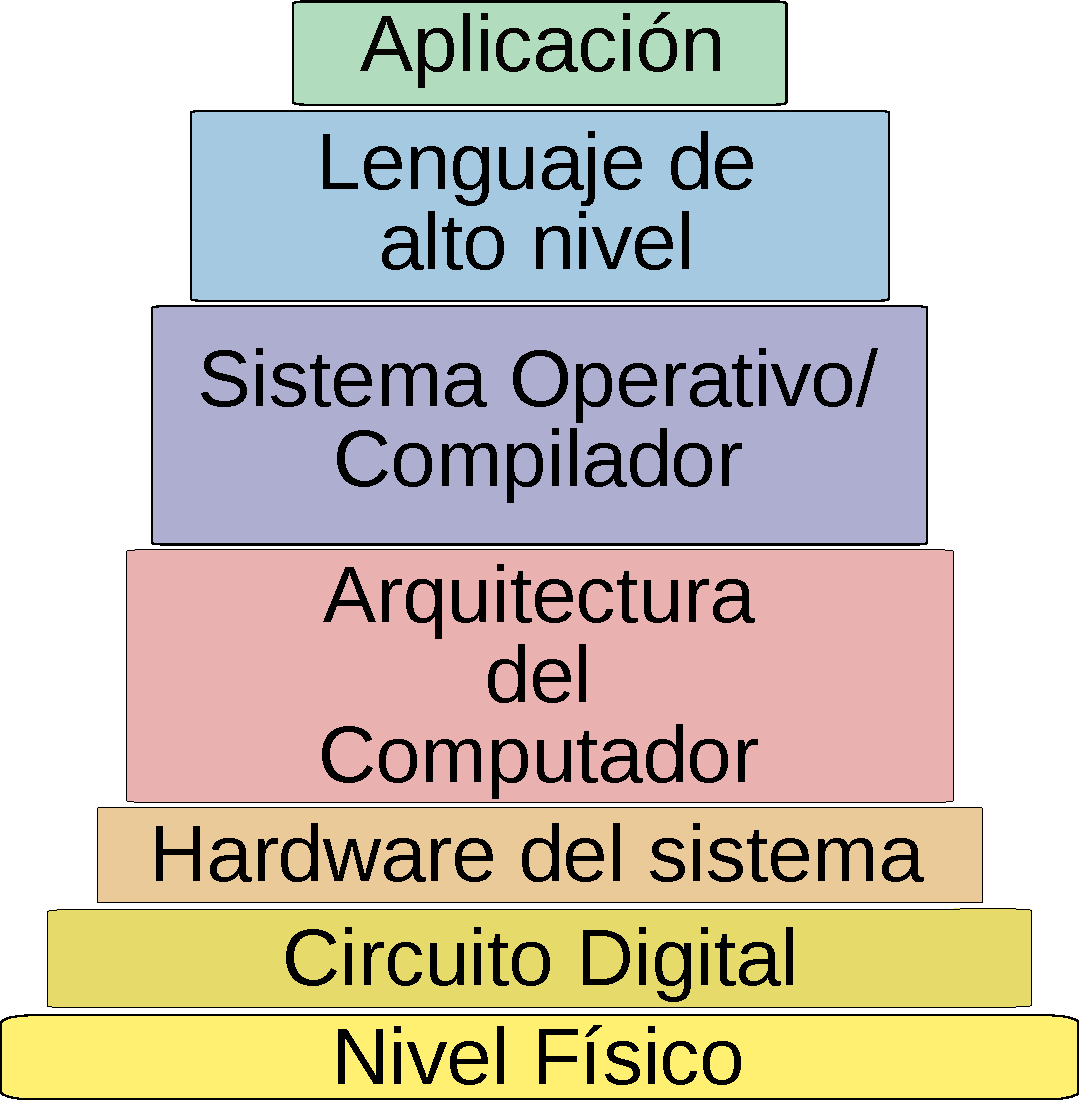
\includegraphics[width=10cm]{nivel_descripcion.pdf}
\begin{tikzpicture}
\draw (0,0)node[rectangle,minimum width=4cm, minimum height=1cm ,rounded corners=3mm,draw = green!50!black!50]{Aplicación};
\draw (0,-1)node[rectangle,minimum width=4.5cm, minimum height=1cm ,rounded corners=3mm,draw = green!50!black!50]{Lenguaje de alto nivel};
\draw (0,-2)node[rectangle,minimum width=5cm, minimum height=1cm ,rounded corners=3mm,draw = green!50!black!]{Sistema operativo/Compilador};
\draw (0,-3)node[rectangle,minimum width=5.5cm, minimum height=1cm ,rounded corners=3mm,draw = green!50!black!50]{Arquitectura del Computador};
\draw (0,-4)node[rectangle,minimum width=6cm, minimum height=1cm ,rounded corners=3mm,draw = green!50!black!50]{Hardware del sistema};
\draw (0,-5)node[rectangle,minimum width=6.5cm, minimum height=1cm ,rounded corners=3mm,draw = green!50!black!50]{Circuito Digital};
\draw (0,-6)node[rectangle,minimum width=7cm, minimum height=1cm ,rounded corners=3mm,draw = green!50!black!50]{Nivel Físico};
\end{tikzpicture}
	\caption{Descripción por niveles de un computador}
	\label{fig:nivel}
\end{figure}
\switchcolumn
Figure \ref{fig:nivel} shows a general computer layout described by levels. Each level lays and assume the previous level. 
\begin{figure}[h]
	\centering
		%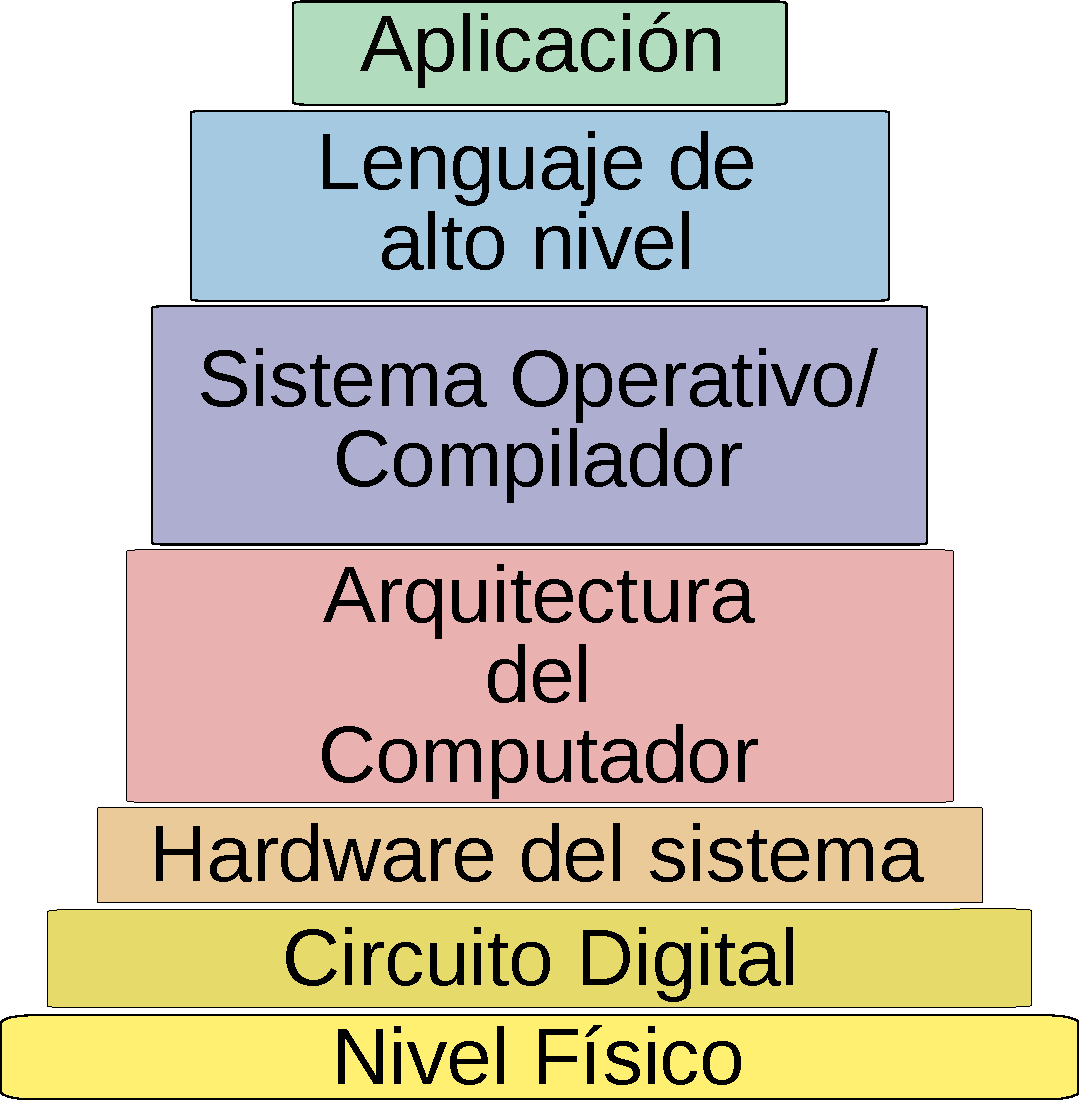
\includegraphics[width=10cm]{nivel_descripcion.pdf}
\begin{tikzpicture}
\draw (0,0)node[rectangle,minimum width=4cm, minimum height=1cm ,rounded corners=3mm,draw = green!50!black!50]{Aplication};
\draw (0,-1)node[rectangle,minimum width=4.5cm, minimum height=1cm ,rounded corners=3mm,draw = green!50!black!50]{High level languaje};
\draw (0,-2)node[rectangle,minimum width=5cm, minimum height=1cm ,rounded corners=3mm,draw = green!50!black!]{operating System/Compiler};
\draw (0,-3)node[rectangle,minimum width=5.5cm, minimum height=1cm ,rounded corners=3mm,draw = green!50!black!50]{Computer Architecture};
\draw (0,-4)node[rectangle,minimum width=6cm, minimum height=1cm ,rounded corners=3mm,draw = green!50!black!50]{Hardware};
\draw (0,-5)node[rectangle,minimum width=6.5cm, minimum height=1cm ,rounded corners=3mm,draw = green!50!black!50]{Digital Circuit};
\draw (0,-6)node[rectangle,minimum width=7cm, minimum height=1cm ,rounded corners=3mm,draw = green!50!black!50]{Physical Level};
\end{tikzpicture}
	\renewcommand{\figurename}{Figure}
	\caption{Computer level description}
	\label{fig:nivel}
\end{figure}
\switchcolumn
\begin{enumerate}
\item \textbf{Nivel Físico.} Constituye la base del \emph{hardware} del computador. Está constituido por los componentes electrónicos básicos, diodos, transistores, resistencias, etc.  En un computador moderno, no es posible separar o tan siquiera observar dichos componentes: Se han fabricado directamente sobre un cristal semiconductor, y forman parte de un dispositivo electrónico conocido con el nombre de circuito integrado.

\item \textbf{Circuito Digital.}
Los componentes del nivel físico se agrupan formando circuitos digitales, (En nuestro caso circuitos digitales integrados). Los circuitos digitales trabajan solo con dos niveles de tensión ($V_1, V_0$) lo que permite emplearlos para establecer relaciones lógicas: $V_1$=verdadero, $V_2$=falso. Estas relaciones lógicas establecidas empleando los valores de la tensión de los circuitos digitales constituyen el soporte de todos los cálculos que el computador puede realizar.

\item \textbf{Organización Hardware del sistema.}\index{Computador ! \emph{hardware}} 
Los circuitos digitales integrados se agrupan y organizan para formar el \emph{Hardware} del ordenador.  Los módulos básicos que constituyen el \emph{Hardware} son la unidad central de procesos (CPU), La unidad de memoria y las unidades de entrada y salida de datos. Dichos componentes están conectados entre sí mediante un bus, que transfiere datos de una unidad a otra.

\item \textbf{Arquitectura del computador.} \index{Computador ! arquitectura}
La arquitectura define cómo trabaja el computador. Por tanto, está estrechamente relacionada con la organización hardware del sistema, pero opera a un nivel de abstracción superior. Establece cómo se accede a los registros de memoria, arbitra el uso de los buses que comunican unos componentes con otros, y regula el trabajo de la CPU.  

Sobre la arquitectura se establece el lenguaje básico en el que trabaja el ordenador, conocido cómo lenguaje máquina. Es un lenguaje que emplea todavía niveles lógicos binarios (ceros o unos) y por tanto no demasiado apto para ser interpretado por los seres humanos. Este lenguaje permite al ordenador realizar operaciones básicas como copiar el contenido de un registro de memoria en otro, sumar el contenido de dos registros de memoria, etc. 

El lenguaje máquina es adecuado para los computadores, pero no para los humanos, por eso, los fabricantes suministran junto con el computador un repertorio básico de instrucciones que su máquina puede entender y realizar en un lenguaje algo más asequible. Se trata del lenguaje ensamblador. Los comandos de éste lenguaje son fácilmente traducibles en una o varias instrucciones de lenguaje máquina.   Aún así se trata de un lenguaje en el que programar directamente resulta una tarea tediosa y proclive a cometer errores. 

\item \textbf{Compiladores y Sistemas Operativos} \index{Sistema operativo} \index{Compilador}
Los Compiladores constituyen un tipo de programas especiales que permiten convertir un conjunto de instrucciones, escritas en un lenguaje de alto nivel en lenguaje máquina. El programador escribe sus instrucciones en un fichero de texto normal, perfectamente legible para el ser humano, y el compilador convierte las instrucciones contenidas en dicho fichero en secuencias binarias comprensibles por la máquina.

Los computadores primitivos solo eran capaces de ejecutar un programa a la vez. A medida que se fueron fabricando ordenadores mas sofisticados, surgió la idea de crear programas que se encargaran de las tareas básicas: gestionar el flujo de información, manejar periféricos, etc. Estos programas reciben el nombre de sistemas operativos. Los computadores modernos cargan al arrancar un sistema operativo que controla la ejecución del resto de las aplicaciones. Ejemplos de sistemas operativos son DOS (Disk Operating System), Unix y su versión para ordenadores personales Linux.

\item \textbf{Lenguajes de alto nivel.} \index{Programación! lenguajes}
Los lenguajes de alto nivel están pensados para facilitar la tarea del programador, desentendiéndose de los detalles de implementación del hardware del ordenador.  Están compuestos por un conjunto de comandos y unas reglas sintácticas, que permiten describir las instrucciones para el computador en forma de texto.

De una manera muy general, se pueden dividir los lenguajes de alto nivel en lenguajes compilados y lenguajes interpretados. Los lenguajes compilados emplean un compilador para convertir los comandos del lenguaje de alto nivel en lenguaje máquina. Ejemplos de lenguajes compilados son C , C++ y Fortran. Los lenguajes interpretados a diferencia de los anteriores no se traducen a lenguaje máquina antes de ejecutarse. Si no que utilizan otro programa --el interprete-- que va leyendo los comandos del lenguaje y convirtiéndolos en instrucciones máquina a la vez que el programa se va ejecutando. Ejemplos de programas interpretado son Basic, Python y Java.

\item \textbf{Aplicaciones.} \index{Programación! aplicaciones} Se suele entender por aplicaciones programas orientados a tareas específicas, disponibles para un usuario final. Habitualmente se trata de programas escritos en un lenguaje de alto nivel y presentados en un formato fácilmente comprensible para quien los usa.

Existen multitud de aplicaciones, entre las más conocidas cabe incluir los navegadores para Internet, como Explorer, Mocilla o Google Crome, los editores de texto, como Word, las hojas de cálculo como Excel o los clientes de correo como Outlook. En realidad, la lista de aplicaciones disponibles en el mercado sería interminable. 
\end{enumerate}

\switchcolumn
\subsection{Computer description levels.}
\begin{enumerate}
\item \textbf{Physical Level.} It's the ground of the computer hardware. Basic electronic components, diodes, transistors, resistances, etc, make it up. In a modern computer, it is impossible to split or event to watch such components: they are built directly in a semiconductor Crystal and part\; of an electronic device Known as \emph{integrated circuit}.

\item \textbf{Digital Circuit.}
Physical level components are grouped, forming digital circuits. (In our case, Integrated digital circuits). They work with only two voltage levels ($V_1, V_0$). This allows us to use them for defining logical relationships: $V_1$=true, $V_2$=false. This logical relationship obtained using two voltage levels of digital circuits is, in turn, the basis for every computing the computer can carry out.

\item \textbf{Computer Hardware organisation.}\index[eng]{Computer ! \emph{hardware}} 
Digital circuits are grouped and organized to build up the computer Hardware. Basic hardware modules are The central processing unit(CPU), the memory unit and the input and output units. These components are connected by a bus, which transfers data from one unit to another.

\item \textbf{Computer Architecture.} \index[eng]{Computer ! architecture}
The architecture defines how the computer works. Thus, it is highly related to the hardware organization of the system; bit architecture works at a higher abstraction level. It defines how to get access to the memory register, arbitrate the use of the buses with links to the different components and regulates the CPU work.   
 
The primary language the computer works with is established according to its architecture. This primary language is called Machine language. It still uses binary logical levels (zeros and ones), so it is unsuitable for being understood by human beings. The computer uses machine language to perform basic operations such as copying the content from one memory register to another, adding the contents of two memory registers, etc.     

Machine language is suitable for computers but not for human beings. Thus, manufacturers supply the computer with a basic repertory of instructions that their machine can understand and carry out, written in a more accessible language. It is known as assembler language. The commands of this language are accessible to translate to one or several machine language instructions. Writing code right in assembler language is tedious and prone to mistakes.     
   
\item \textbf{Compilers y operating Systems} \index[eng]{operating system} \index[eng]{Compiler}
Compilers are special programs that allow us to translate instructions written in a high-level language into machine language. The programmer writes instructions in plain text, readable for a human being. Then, the compiler translates the file's contents into binary sentences that the machine can interpret.
       
Early computers were only able to run a program at a time. As new and more sophisticated computers were built, it arises the idea of making programs which were able to take over the basic tasks:
Managing the information flow, dealing with peripheral devices, etc. These programs are called operating systems. Modern computers load an operating system at the boot time, which controls the running of the remaining programs. Some examples of operating systems are DOS (Disk Operating System), UNIX and the UNIX version for personal computers LINUX.       

\item \textbf{High level languages} \index[eng]{Programming! languages}
High-level languages are intended to make the programmer's work easier, ignoring the hardware implementation details.   They comprise a set of commands and syntactic rules, allowing the programmer to describe computer instruction in plain text.

Generally, High-level languages can be divided into compiled and interpreted languages. Compiled languages employ a compiler to traduce the command from the high-level language to machine language. Some examples are C, C++ and FORTRAN. On the contrary, interpreted languages do not translate to machine language. They use a second program known as the interpreter. While a program in the interpreted language is running, the interpreter reads the program commands one by one and translates them to machine language. Examples of interpreted languages are BASIC, Python or Java.  


\item \textbf{Programmes.} \index[eng]{Programming! Programmes} 
A Programme is a piece of code intended to perform specific tasks. They are available to the final users of the computer. Usually, programs are written using a high-level language and are user-friendly, i.e. they have an interface that is easy to use.

There are many different kinds of programs, according to their purpose. We can find Internet web browsers like Google Chrome, Mozilla or Explorer, text editors like Word, Emacs or Latex.    
E-mail clients (Mail User Agents) like Outlook or Mozilla Thunderbird. The list of available programs would be endless. 
\end{enumerate}

\end{paracol}


\subsection{El modelo de computador de Von Neumann \\ The Von Neumann's computer model} \index{Von Neumann}

\begin{paracol}{2}
Los computadores modernos siguen, en lineas generales, el modelo propuesto por Von Neumann.  La figura \ref{fig:vonn} muestra un esquema de dicho modelo. 

\begin{figure}[h]
	\centering
	\begin{tikzpicture}
\draw (0,0)node[rectangle,minimum width=7cm, minimum height=7cm ,rounded corners=3mm,draw = green!50!black!50]{};
\draw (-0.25,2.7)node[rectangle,minimum width=6cm, minimum height=0.6cm ,rounded corners=3mm,draw = green!50!black!50]{Unidad de Control (UC)};
\draw (-1.75,2)node[rectangle,minimum width=2.5cm, minimum height=0.25cm ,draw = green!50!black!50]{};
\draw (-1.75,1.5)node[rectangle,minimum width=2.5cm, minimum height=0.25cm , draw = green!50!black!50]{};
\draw (-1.75,1)node[rectangle,minimum width=2.5cm, minimum height=0.25cm, draw = green!50!black!50]{};
\draw (-1.75,0.5)node[rectangle,minimum width=2.5cm, minimum height=0.25cm ,draw = green!50!black!50]{};
\draw (-1.75,0)node[rectangle,minimum width=2.5cm, minimum height=0.25cm ,draw = green!50!black!50]{};
\draw (-1.75,-0.5)node[rectangle,minimum width=2.5cm,minimum height=0.25cm ,draw = green!50!black!50]{};
\draw (-1.75,-0.5)node[rectangle,minimum width=2.5cm,minimum height=0.25cm]{Registros};
\draw (-1.75,-1)node[rectangle,minimum width=2.5cm, minimum height=0.25cm,,draw = green!50!black!50]{};
\draw (-1.75,-1.5)node[rectangle,minimum width=2.5cm, minimum height=0.25cm , draw = green!50!black!50]{};
\draw (-1.75,-2)node[rectangle,minimum width=2.5cm, minimum height=0.25cm, draw = green!50!black!50]{};
\draw (-1.75,-2.5)node[rectangle,minimum width=2.5cm, minimum height=0.25cm ,draw = green!50!black!50]{};
\draw (-1.75,-3)node[rectangle,minimum width=2.5cm, minimum height=0.25cm ,draw = green!50!black!50]{};
\draw (1.65,2)node[rectangle,minimum width=2.5cm, minimum height=0.25cm]{Cont. Prog. (PC)};
\draw (1.65,1.5)node[rectangle,minimum width=2.5cm, minimum height=0.25cm]{Reg Estado (SR)};
\draw (1.65,0)node[rectangle,minimum width=2.5cm, minimum height=0.25cm, rounded corners=3mm ,draw = green!50!black!50,align=center]{Unidad \\ Aritmético \\ Lógica\\ (ALU)};
\draw (1.65,-1.5)node[rectangle,minimum width=2.5cm, minimum height=0.25cm]{Reg. Instr (IR)};
\draw (1.65,-2)node[rectangle,minimum width=2.5cm, minimum height=0.25cm]{Reg. Dir. Mem. (MAR)};
\draw (1.65,-2.5)node[rectangle,minimum width=2.5cm, minimum height=0.25cm]{Reg. Dat. Mem. (MDR)};
\draw (2.5,-3.25)node[rectangle,minimum width=2.5cm, minimum height=0.25cm]{\textbf{CPU}};
\draw[latex-latex](0.5,-3.5)--(0.5,-4);
\draw[latex-latex](0.75,-3.5)--(0.75,-4.7);
\draw[latex-latex](1,-3.5)--(1,-5.4);
\draw[latex-latex](-3.5,-4)node[anchor=south west]{Bus datos}--(3.5,-4);
\draw[latex-latex](-3.5,-4.7)node[anchor=south west]{Bus direcc.}--(3.5,-4.7);
\draw[latex-latex](-3.5,-5.4)node[anchor=south west]{Bus control}--(3.5,-5.4);

\draw (-1.65,-6.5)node[rectangle,minimum width=2.5cm, minimum height=1cm, rounded corners=3mm ,draw = green!50!black!50,align=center]{Memoria};
\draw (1.65,-6.5)node[rectangle,minimum width=2.5cm, minimum height=1cm, rounded corners=3mm ,draw = green!50!black!50,align=center]{E/S)};
\draw[latex-latex](-0.7,-5.4)--(-0.7,-6);
\draw[latex-latex](-0.9,-4.7)--(-0.9,-6);
\draw[latex-latex](-1.1,-4)--(-1.1,-6);

\draw[latex-latex](2.6,-5.4)--(2.6,-6);
\draw[latex-latex](2.4,-4.7)--(2.4,-6);
\draw[latex-latex](2.2,-4)--(2.2,-6);
\end{tikzpicture}	
	\caption{Modelo de Von Neumann}
	\label{fig:vonn}
\end{figure}

\switchcolumn
Modern computers generally follow the model proposed by Von Neumann. Figure \ref{fig:vonn} shows a schematic view of Von Neumann's model.  
\begin{figure}[h]
	\centering
	\begin{tikzpicture}
\draw (0,0)node[rectangle,minimum width=7cm, minimum height=7cm ,rounded corners=3mm,draw = green!50!black!50]{};
\draw (-0.25,2.7)node[rectangle,minimum width=6cm, minimum height=0.6cm ,rounded corners=3mm,draw = green!50!black!50]{Control Unit (UC)};
\draw (-1.75,2)node[rectangle,minimum width=2.5cm, minimum height=0.25cm ,draw = green!50!black!50]{};
\draw (-1.75,1.5)node[rectangle,minimum width=2.5cm, minimum height=0.25cm , draw = green!50!black!50]{};
\draw (-1.75,1)node[rectangle,minimum width=2.5cm, minimum height=0.25cm, draw = green!50!black!50]{};
\draw (-1.75,0.5)node[rectangle,minimum width=2.5cm, minimum height=0.25cm ,draw = green!50!black!50]{};
\draw (-1.75,0)node[rectangle,minimum width=2.5cm, minimum height=0.25cm ,draw = green!50!black!50]{};
\draw (-1.75,-0.5)node[rectangle,minimum width=2.5cm,minimum height=0.25cm ,draw = green!50!black!50]{};
\draw (-1.75,-0.5)node[rectangle,minimum width=2.5cm,minimum height=0.25cm]{Registers};
\draw (-1.75,-1)node[rectangle,minimum width=2.5cm, minimum height=0.25cm,,draw = green!50!black!50]{};
\draw (-1.75,-1.5)node[rectangle,minimum width=2.5cm, minimum height=0.25cm , draw = green!50!black!50]{};
\draw (-1.75,-2)node[rectangle,minimum width=2.5cm, minimum height=0.25cm, draw = green!50!black!50]{};
\draw (-1.75,-2.5)node[rectangle,minimum width=2.5cm, minimum height=0.25cm ,draw = green!50!black!50]{};
\draw (-1.75,-3)node[rectangle,minimum width=2.5cm, minimum height=0.25cm ,draw = green!50!black!50]{};
\draw (1.65,2)node[rectangle,minimum width=2.5cm, minimum height=0.25cm]{Prog. Count. (PC)};
\draw (1.65,1.5)node[rectangle,minimum width=2.5cm, minimum height=0.25cm]{Stat. Reg (SR)};
\draw (1.65,0)node[rectangle,minimum width=2.5cm, minimum height=0.25cm, rounded corners=3mm ,draw = green!50!black!50,align=center]{Arithmetic \\ Logic\\ UNIT\\ (ALU)};
\draw (1.65,-1.5)node[rectangle,minimum width=2.5cm, minimum height=0.25cm]{Instr. Reg (IR)};
\draw (1.65,-2)node[rectangle,minimum width=2.5cm, minimum height=0.25cm]{Mem. Adr. Reg. (MAR)};
\draw (1.65,-2.5)node[rectangle,minimum width=2.5cm, minimum height=0.25cm]{Mem. Dat. Reg. (MDR)};
\draw (2.5,-3.25)node[rectangle,minimum width=2.5cm, minimum height=0.25cm]{\textbf{CPU}};
\draw[latex-latex](0.5,-3.5)--(0.5,-4);
\draw[latex-latex](0.75,-3.5)--(0.75,-4.7);
\draw[latex-latex](1,-3.5)--(1,-5.4);
\draw[latex-latex](-3.5,-4)node[anchor=south west]{Bus datos}--(3.5,-4);
\draw[latex-latex](-3.5,-4.7)node[anchor=south west]{Bus direcc.}--(3.5,-4.7);
\draw[latex-latex](-3.5,-5.4)node[anchor=south west]{Bus control}--(3.5,-5.4);

\draw (-1.65,-6.5)node[rectangle,minimum width=2.5cm, minimum height=1cm, rounded corners=3mm ,draw = green!50!black!50,align=center]{Memoria};
\draw (1.65,-6.5)node[rectangle,minimum width=2.5cm, minimum height=1cm, rounded corners=3mm ,draw = green!50!black!50,align=center]{E/S)};
\draw[latex-latex](-0.7,-5.4)--(-0.7,-6);
\draw[latex-latex](-0.9,-4.7)--(-0.9,-6);
\draw[latex-latex](-1.1,-4)--(-1.1,-6);

\draw[latex-latex](2.6,-5.4)--(2.6,-6);
\draw[latex-latex](2.4,-4.7)--(2.4,-6);
\draw[latex-latex](2.2,-4)--(2.2,-6);
\end{tikzpicture}	
	\caption{Von Neumann's model}
	\label{fig:vonn}
\end{figure}

\switchcolumn
En el modelo de Von Newman se pueden  distinguir tres módulos básicos y una serie de elementos de interconexión.  Los módulos básicos son: 

\begin{itemize}
\item \textbf{La Unidad Central de Procesos.} CPU \index{CPU} (\emph{Central process unit)}) , esta unidad constituye el núcleo en el que el ordenador realiza las operaciones. 

Dentro de la CPU pueden a su vez distinguirse las siguientes partes:

\begin{itemize}

\item La unidad de proceso ó ruta de datos: Está formada por La Unidad Aritmético Lógica (ALU), \index{ALU} capaz de realizar las operaciones aritméticas y lógicas que indican las instrucciones del programa. En general las ALUs se construyen para realizar aritmética entre enteros, y realizar las operaciones lógicas básicas del algebra de Boole (AND, OR, etc). Habitualmente, las operaciones para números no enteros, representados en \emph{punto flotante} se suelen realizar empleando un procesador específico que se conoce con el nombre de Coprocesador matemático. La velocidad de procesamiento suele medirse en millones de operaciones por segundo (MIPS) o millones de operaciones en punto flotante por segundo (MFLOPS).

\item El banco de registros: Conjunto de registros en los que se almacenan los datos con los que trabaja la ALU y los resultados obtenidos.
 
\item La unidad de control (UC) o ruta de control: se encarga de buscar las instrucciones en la memoria principal y guardarlas en el registro de instrucciones, las decodifica, las ejecuta empleando la ALU, guarda los resultados en el registro de datos, y guarda las condiciones derivadas de la operación realizada en el registro de estado.  El registro de datos de memoria, contiene los datos que se están leyendo de la memoria principal o van a escribirse en la misma. El registro de direcciones de memoria, guarda la dirección de la memoria principal a las que esta accediendo la ALU, para leer o escribir. El contador del programa, también conocido como puntero de instrucciones, es un registro que guarda la posición en la que se encuentra la CPU dentro de la secuencia de instrucciones de un programa.
\end{itemize}
 

\item \textbf{La unidad de memoria.} Se trata de la memoria principal o primaria del computador.  Está dividida en bloques de memoria que se identifican mediante una dirección. La CPU tiene acceso directo a dichos bloques de memoria.

La unidad elemental de información digital es el bit \index{bit} (0,1). La capacidad de almacenamiento de datos se mide en Bytes \index{Byte} y en sus múltiplos, calculados siempre como potencias de 2:

\begin{align} \nonumber
1\  Byte = &\ 8\ bits\ &\  \\ \nonumber
1\  KB  = &\ 2^{10}\ bits=1024\ B&\ \\  \nonumber
1\  MB = &\ 2^{20}\ bits=1024\ KB&\ \\  \nonumber
1\  GB = &\ 2^{30}\ bits &\ \\  \nonumber
1\  TB  = &\ 2^{40}\ bits\ &\
\end{align} 

\item \textbf{Unidad de Entrada/Salida.} Transfiere información entre el computador y los dispositivos periféricos.
\end{itemize}

Los elementos de interconexión se conocen con el nombre de \emph{Buses}. Se pueden distinguir tres: En bus de datos, por el que se transfieren datos entre la CPU y la memoria ó la unidad de entrada/salida. El bus de direcciones, par especificar una dirección de memoria o del registro de E/S. Y el bus de Control, por el que se envían señales de control, tales como la señal de reloj, la señal de control de lectura/escrituras entre otras.

\switchcolumn
Von Neuman's model has been divided into three basic models and several interconnection elements. The basic modules are: 

\begin{itemize}
\item \textbf{The Central Processing Unity.} CPU \index{CPU} This Unity is the kernel where the computer performs operations. 

Inside the CPU, it is possible to difference the following parts:

\begin{itemize}

\item The processing unit or data router comprises the Arithmetic Logic Unit (ALU), \index{ALU}. The ALU can perform the arithmetical and logical operations described in the program instructions. They are built to perform arithmetic between integer numbers and the basic Boole's algebra logical operations (AND, OR, etc). Non-integer numbers are usually represented using a unique format called \emph{floating point representation}. Operations between floating point numbers are performed using a specific processor known as a coprocessor. The processing speed is measured in millions of instructions per second (MIPS) or millions of floating point operations per second (MFLOPS).

\item The register bank: A set of registers for storing the data ALU is working with and the results of ALU operations.
 
\item The control unit (UC) or control route: It fetches the instructions from the main memory and stores them in the instruction register. It also decoded the instructions, executed them using the ALUs, and stored the results in the data register. Once the operation is finished, the UC stores the conditions derived from the operation in the state register. The memory data register holds the data read from the main memory or those ready to be written there. Memory Address register holds the main memory address the ALU is accessing for writing or reading. The programme counter, or the instruction pointer, is a special register. It stores the current position at which the CPU is located inside a program instructions sequence.    
\end{itemize}
 

\item \textbf{Memory Unit} It is the main or primary memory of the computer. It is divided into memory blocks. Each memory block is identified by its address. The CPU has direct access to memory blocks.

The elemental unit of digital information is the \emph{bit} \index{bit}(0,1). Data storing capacity is gauged in Bytes \index{Byte} and multiples of Byte, represented as powers of two:

\begin{align} \nonumber
1\  Byte = &\ 8\ bits\ &\  \\ \nonumber
1\  KB  = &\ 2^{10}\ bits=1024\ B&\ \\  \nonumber
1\  MB = &\ 2^{20}\ bits=1024\ KB&\ \\  \nonumber
1\  GB = &\ 2^{30}\ bits &\ \\  \nonumber
1\  TB  = &\ 2^{40}\ bits\ &\
\end{align} 

\item \textbf{Input/Output Unit}. This unit transfers information between the computer and the peripheral devices.
\end{itemize}

The interconnection elements are called \emph{Buses}. We can define three: the data bus transfers data between the CPU and the main memory or the input/output unity. The address bus is used for transmitting a memory address or an input/output unit. The control bus for sending control signals, such as the clock signal and the reading/writing control signal, among others.     
\end{paracol} 


\begin{paracol}{2}
\subsection{Representación binaria} \index{Base 2}
Veamos con algo más de detalle, cómo representa la información un computador. Como se explicó anteriormente, La electrónica que constituye la parte física del ordenador, trabaja con dos niveles de voltaje. Esto permite definir dos estados, --alto, bajo-- que pueden representarse dos símbolos  $0$ y $1$. Habitualmente, empleamos $10$ símbolos: \\${0,1,2,3,4,5,6,7,8,9}$, es decir, empleamos una representación decimal. Cuando queremos representar números mayores que nueve, dado que hemos agotado el número de dígitos disponibles, lo que hacemos es combinarlos, agrupando cantidades de diez en diez. Así por ejemplo, el numero $16$, representa seis unidades más un grupo de diez unidades y el número $462$ representa dos unidades más seis grupos de diez unidades más cuatro grupos de 10 grupos de 10 unidades.  Matemáticamente, esto es equivalentes a emplear sumas de dígitos por potencias de diez:
\switchcolumn
\subsection{Binary coding} \index[eng]{Base 2}

Let's see in more detail how a computer represents the information. As described before, the electronic stuff represents the computer's physical part. It works with two voltage levels, which can be associated with two states ---high and low--- and, in turn, these levels can define two symbols, $0$ and $1$. Usually, we employ $10$ symbols (digits):\\ ${0,1,2,3,4,5,6,7,8,9}$, i.e. we use a \emph{decimal} representation. Whenever we want to represent a number greater than nine, we combine several symbols, gathering quantities in groups of ten because we have exhausted the ten available digits. So, for instance,  the number $16$ represents six units plus a group of ten units, and the number $462$ represents two units plus six groups of ten units, plus four groups of ten groups of 10 units. In mathematics, this is equal to using sums of products of digits by powers of ten:       

\end{paracol}
\begin{equation*}
13024 = 1\times10^4+3\times10^3+0\times10^2+2\times10^1+4\times10^0 
\end{equation*}

\begin{paracol}{2}
Si recorremos los dígitos que componen el número de izquierda derecha, cada uno de ellos representa una potencia de diez superior, porque cada uno representa la cantidad de grupos de 10 grupos, de grupos ... de diez grupos de unidades. Esto hace que potencialmente podamos representar cantidades tan grandes como queramos, empleando tan solo diez símbolos. Esta representación, a la que estamos habituados recibe el nombre de representación en base 10 \index{Base 10}. Pero no es la única posible.

\switchcolumn
If we look at the digits that compose the number from left to right, each one represents an upper power of ten, i.e., each represents the number of groups of ten groups of groups ... of ten groups of unities. This means we can represent amounts as significant as we wish, using only ten symbols. We are used to this numerical representation, which is known as a decimal representation or representation in base $10$. But it is not the only one.   

\switchcolumn
Volvamos a la representación empleada por el computador. En este caso solo tenemos dos símbolos distintos el $0$ y el $1$. Si queremos emplear una representación análoga a la representación en base diez, deberemos agrupar ahora las cantidad en grupos de dos. Así los únicos números que admiten ser representados con un solo dígito son el uno y el cero. Para representar el número dos, necesitamos agrupar: tendremos $0$ unidades y $1$ grupo de dos, con lo que la representación del número dos en base dos será $10$. Para representar el número tres, tendremos una unidad más un grupo de dos, por lo que la representación será $11$, y así sucesivamente. Matemáticamente esto es equivalente emplear sumas de dígitos por potencias de 2:

\switchcolumn
Returning to the computer's numerical representation, we have only two digits: $0$ and $1$. If we want to define a representation that resembles the base $10$ representation, we must now gather the quantities in groups of two. So, the number two is represented in base $2$ as $10$. To represent the number three, we have a group of two plus one unit $11$. In mathematics, this is equal to using sums of products of digits by powers of two;               
\end{paracol}

\begin{equation*}
10110 = 1\times2^4+0\times2^3+1\times2^2+1\times2^1+0\times2^0 
\end{equation*}
\begin{paracol}{2}
Esta representación recibe el nombre de representación binaria o en base 2.
\index{Conversión! binario a decimal}La expansión de un número representado en binario en potencias de 2, nos da un método directo de obtener su representación decimal. Así, para el ejemplo anterior, si calculamos las potencias de dos y sumamos los resultados obtenemos:
\switchcolumn
This representation is known as binary coding. \index{Conversion! binary to decimal} If we expand the binary encoding of a number as powers of two, we obtain a direct way to obtain its decimal representation. For instance, If we take the last example, calculate the power of two and add the results we obtain,
\end{paracol}
  \begin{equation*} 1\times2^4+0\times2^3+1\times2^2+1\times2^1+0\times2^0=16+0+4+2+0=22 
\end{equation*}
\begin{paracol}{2}
que es la representación en base 10 del número binario $10110$.
\switchcolumn
which is the representation on base 10 for the binary number $10110$
\end{paracol}
\begin{paracol}{2}
Para números no enteros, la representación tanto en decimal como en binario, se extiende de modo natural empleando potencias negativas de 10 y de 2 respectivamente. Así,
\switchcolumn
For non-integer numbers, decimal and binary representations of a number extend straightforwardly using the negative powers of 10 and 2, respectively. So,   
\end{paracol}
\begin{equation} \nonumber
835.41 = 8\times10^2+3\times10^1+5\times10^0+4\times10^{-1}+1\times10^{-2} 
\end{equation}
\begin{paracol}{2}
y para un número en binario,
\switchcolumn
and for a binary number,
\end{paracol}

\begin{equation} \nonumber
101.01 = 1\times2^2+0\times2^1+1\times2^0+0\times2^{-1}+1\times2^{-2} 
\end{equation}

De nuevo, basta calcular el término de la derecha de la expresión anterior para obtener la representación decimal del número $101.01$.

\index{Conversión! decimal a binario. números enteros}¿Cómo transformar la representación de un número de decimal a binario? De nuevo nos da la clave la representación en sumas de productos de dígitos por potencias de dos. Empecemos por el caso de un número entero. Supongamos un número D, representado en decimal. Queremos expandirlo en una suma de potencias de dos. Si dividimos el número por 2, podríamos representarlo cómo:
 
\begin{equation*}
\label{eq:1}
D=2\cdot C_1+R_1
\end{equation*}

donde $C_1$ representa el cociente de la división y $R_1$ el resto. Como estamos dividiendo por dos, el resto solo puede valer cero o uno. Supongamos ahora que volvemos a dividir el cociente obtenido por dos,

 \begin{equation*}
 \label{eq:2}
C_1=2\cdot C_2+R_2 \
\end{equation*}

Si sustituimos el valor obtenido para $C_1$ en la ecuación inicial obtenemos,   
\begin{equation*}
D=2\cdot(2\cdot C_2+R_2)+R_1= 2^2\cdot C_2+R_2\cdot 2^1+R_1\cdot 2^0 
\end{equation*}

Si volvemos a dividir el nuevo cociente obtenido $C_2$ por dos, y volvemos a sustituir,

 \begin{align*}
C_2&=2\cdot C_3+R_3 \\
D&=2^2\cdot(2\cdot C_3+R_3)+R_2\cdot 2^1+R_1\cdot 2^0=2^3\cdot C_3+R_3\cdot 2^2 +R_2\cdot 2^1+R_1\cdot 2^0
\end{align*}

Supongamos que tras repetir este proceso $n$ veces, obtenemos un conciente $C_n=1$. Lógicamente no tiene sentido seguir dividiendo ya que a partir de este punto, cualquier división posterior que hagamos nos dará cociente $0$ y resto igual a $C_n$. Por tanto, 

 \begin{align*}
D&=1\cdot 2^n+R_n\cdot 2^{n-1}\cdots +R_3\cdot 2^2 +R_2\cdot 2^1+R_1\cdot 2^0
\end{align*}

La expresión obtenida, coincide precisamente con la expansión en potencias de dos del número binario $1R_n \cdots R_3R_2R_1$.


Como ejemplo,podemos obtener la representación en binario del número $234$, empleando el método descrito: vamos dividiendo el número y los cocientes sucesivos entre dos, hasta obtener un cociente igual a uno y a continuación, construimos la representación binaria del número colocando por orden, de derecha a izquierda.  los restos  obtenidos de las sucesivas divisiones y añadiendo un uno más a la izquierda de la cifra construida con los restos:

\begin{table}[h]
\begin{tabular}{|r|r|r|r|}
Dividendo& &Cociente $\div 2$&Resto\\
\hline
234& &117&0\\
117& &58&1\\
58& &29&0\\
29& &14&1\\
14& &7&0\\
7& &3&1\\
3& &1&1
\end{tabular}
\end{table}
 
 Por tanto, la representación en binario de 234 es 11101010.
 
\index{Conversión! decimal a binario, números no entero}Supongamos ahora un número no entero, representado en decimal, de la forma $0,d$ . Si lo multiplicamos por dos:

\begin{equation}
E_1,d_1=0,d\cdot 2
\end{equation}
Donde $E_1$ representa la parte entera y $d_1$ la parte decimal del número calculado.
Podemos entonces representar $0,d$ como,
\begin{equation}
\label{eq:5}
0,d=(E_1,d_1)\cdot 2^{-1}=E_1\cdot 2^{-1}+0,d_1\cdot 2^{-1}
\end{equation}  

Si volvemos a multiplicar $0,d_1$ por dos,

\begin{equation}
E_2,d_2 = 0,d_1\cdot 2
\end{equation}

\begin{equation}
0,d_1=E_2\cdot 2^{-1}+0,d_2\cdot 2^{-1}
\end{equation}  

y sustituyendo en \ref{eq:5}

\begin{equation}
0,d=E_1\cdot 2^{-1}+E_2\cdot 2^{-2}+0,d_2\cdot 2^{-2}
\end{equation}

¿Hasta cuando repetir el proceso? En principio hasta que obtengamos un valor cero para la parte decimal, $0,d_n=0$. Pero esta condición puede no cumplirse nunca. Puede darse el caso --de hecho es lo más probable-- de que un número que tiene una representación exacta en decimal, no la tenga en binario. El criterio para detener el proceso será entonces obtener un determinado número de decimales o bien seguir el proceso hasta que la parte decimal obtenida vuelva a repetirse. Puesto que los ordenadores tienen un tamaño de registro limitado, también está limitado el número de dígitos con el que pueden representar un número decimal. Por eso, lo habitual será truncar el número asumiendo el error que se comete al proceder así.  De este modo, obtenemos la expansión del número original en potencias de dos,

\begin{equation}
0,d\cdot 2=E_1\cdot 2^{-1}+E_2\cdot 2^{-2}+\cdots+ E_n\cdot 2^{-3}+\cdots
\end{equation} 

Donde los valores $E_1\cdots E_n$ son precisamente los dígitos correspondientes a la representación del número en binario: $0.E_1E_2\cdots E_n$. (Es trivial comprobar que solo pueden valer $0$ ó $1$).


Veamos un ejemplo de cada caso, obteniendo la representación binaria del número $0,625$, que tiene representación exacta, y la del número $0,626$, que no la tiene. En este segundo caso, calcularemos una representación aproximada, tomando 8 decimales.

\begin{table}[h]
\begin{tabular}{|r|r|r|r|r r|r|r|r|r|}
P decimal& &$\times 2$& P entera& &&P decimal& &$\times 2$& P entera\\
\cline{1-4}
\cline{7-10}
0,625& &1,25&1& &&0,623& &1,246&1\\
0,25  & &0,5  &0& &&0,246& &0,492&0\\
0,5    & &1,0  &1& &&0,492& &0,984&0\\
         & &       &  & &&0,984& &1,968&1\\
         & &       &  & &&0,968& &1,936&1\\
         & &       &  & &&0,936& &1,872&1\\
         & &       &  & &&0.872& &1.744&1\\
         & &       &  & &&0.744& &1.488&1\\
\end{tabular}
\end{table}

Para construir la representación binaria del primero de los números, nos basta tomar las partes enteras obtenidas, por orden, de derecha a izquierda y añadir un $0$ y la coma decimal a la izquierda. Por tanto  la representación binaria de $0,625$ es $0,101$.  Si expandimos su valor en potencias de dos, volvemos a recuperar el número original en su representación decimal.

 En el segundo caso, la representación binaria, tomando nueve decimales de $0,623$ es $0.10011111$. Podemos calcular el error que cometemos al despreciar el resto de los decimales, volviendo a convertir el resultado obtenido a su representación en base diez,

 \begin{equation*}
0\cdot 2^{0}+1\cdot 2^{-1}+0\cdot 2^{-2}+ 0\cdot 2^{-3}+1\cdot 2^{-4}+1\cdot 2^{-5}+ 1\cdot 2^{-6}+1\cdot 2^{-7}+1\cdot 2^{-8}=0,62109375
\end{equation*} 

El error cometido es, en este caso: $\text{Error}=0,623-0,62109375=0,00190625$.
  
 \section{Aplicaciones de Software Científico}
Dentro del mundo de las aplicaciones, merecen una mención aparte las dedicadas al cálculo científico, por su conexión con la asignatura. 

Es posible emplear lenguajes de alto nivel para construir rutinas y programas que permitan resolver directamente un determinado problema de cálculo. En este sentido, el lenguaje FORTRAN se ha empleado durante años para ese fin, y todavía sigue empleándose en muchas disciplinas científicas y de la Ingeniería.  Sin embargo, hay muchos aspectos no triviales del cálculo con un computador, que obligarían al científico que tuviera que programar sus propios programas a ser a la vez un experto en computadores.  Por esta razón, se han ido desarrollando aplicaciones específicas para cálculo científico que permiten al investigador centrarse en la resolución de su problema y no en el desarrollo de la herramienta adecuada para resolverlo.  
 
En algunos casos, se trata de aplicaciones a medida, relacionadas directamente con algún área científica concreta. En otros, consisten en paquetes de funciones específicos para realizar de forma eficiente determinados cálculos, como por ejemplo
el paquete SPSS para cálculo estadístico.

Un grupo especialmente interesante lo forman algunos paquetes de software que podríamos situar a mitad de camino entre los lenguajes de alto nivel y las aplicaciones: Contienen extensas librerías de funciones, que pueden ser empleadas de una forma directa para realizar cálculos y además permiten realizar programas específicos empleando su propio lenguaje. Entre estos podemos destacar Mathematica, Maple , Matlab, Octave y Scilab y Python. El uso de estas herramientas se ha extendido enormemente en la comunidad científica. Algunas como Matlab  constituyen casi un estándar en determinadas áreas de conocimiento.

 


    

 

  

\chapter{Introducción a la programación en Paython\\ Introduction to Python programming}  \index{Python}
Este capítulo presenta una introducción general a la programación. Para su desarrollo, vamos a emplear una de las aplicaciones informáticas para cálculo científico que más aceptación ha tenido en los últimos años: el entorno de programación de Matlab. Matlab es el acrónimo de MATrix LABboratory. El nombre está relacionado con el empleo de matrices como elemento básico para el cálculo numérico.

Usaremos esta herramienta, entre otras motivos, porque nos ofrece la posibilidad de realizar programas similares a los que podríamos desarrollar con un lenguaje de programación de alto nivel, nos permite resolver problemas de cálculo científico directamente, empleando las herramientas que incluye y, además, nos permite combinar ambas cosas.

Este capítulo no pretende ser exhaustivo, --cosa que por otro lado resulta imposible en el caso de Matlab--, sino tan solo dar una breve introducción a su uso. Afortunadamente, Matlab cuenta con una muy buena documentación, accesible a través de la 'ayuda', eso sí, en inglés. 



\section{El entorno de programación de Matlab}\index{Matlab! entorno de programación}\index{Matlab! IDE}
Cuando iniciamos Matlab en el computador, se abre una ventana formada por uno o más paneles. Esta ventana, constituye lo que en programación se  llama un entorno de desarrollo integrado o, abreviadamente, IDE (acrónimo tomado de su nombre en Inglés: \emph{integrated development environment}. El IDE de Matlab, contiene todo los elementos necesarios para programar. La figura \ref{fig:ide} muestra el aspecto del IDE de Matlab.

\begin{figure}[h]
	\centering
		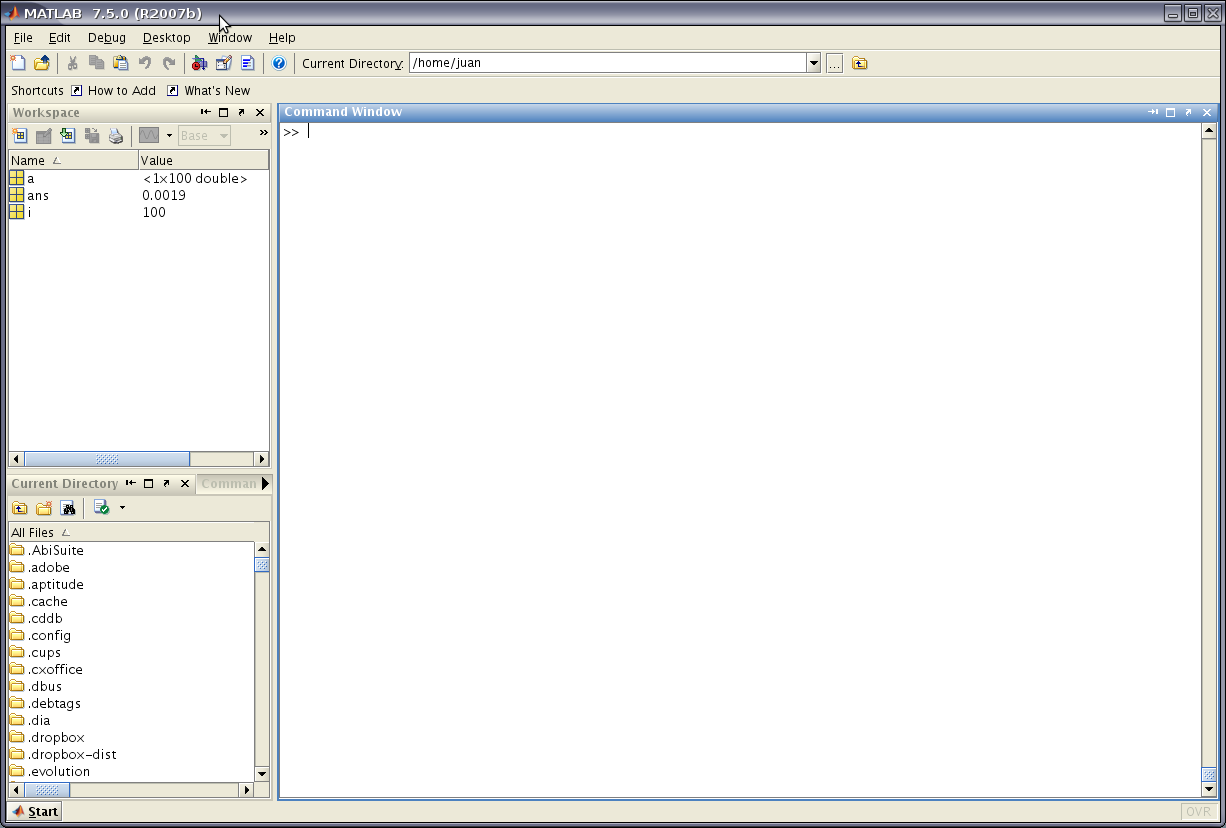
\includegraphics[width=10cm]{ide.png}
	\caption{Entorno de desarrollo integrado de Matlab}
	\label{fig:ide}
\end{figure}

Según como se configure, el IDE de Matlab puede mostrar un número mayor o menor de paneles y una disposición de los mismos distinta a la mostrada en la figura. La mejor manera de aprender estos y otros detalles del IDE es usarlo. Aquí nos centraremos solo en algunos aspectos fundamentales.

\subsection{La ventana de comandos de Matlab} \index{Matlab!ventana de Commandos}
De los paneles mostrados en la ventana de la figura \ref{fig:ide}, vamos a empezar examinando el situado a la derecha. Se trata de la ventana de comandos (\emph{command window}) de Matlab.  \index{prompt} La ventana muestra el simbolo $>>$, que recibe el nombre de \emph{prompt} y, a continuación, una barra vertical $|$ parpadeante.  La ventana de comandos permite al usuario interactuar directamente con Matlab: Matlab puede recibir instrucciones directamente a través de la ventana de comandos, ejecuta las instrucciones recibidas, y devuelve los resultados de nuevo en la ventana de comandos. Veamos un ejemplo muy sencillo: si escribimos en la ventana de comandos:

\begin{verbatim}
>> a=18 + 3
\end{verbatim}

Matlab calcula la suma pedida, devuelve el resultado y, por último, vuelve a presentar el \emph{prompt}, para indicarnos que está preparado para recibir otro comando.

\begin{verbatim}
a =

    21

>> 
\end{verbatim}

De este modo, podemos emplear Matlab de un modo análogo a como emplearíamos una calculadora: realizamos una operación, obtenemos el resultado, realizamos otra operación, obtenemos el resultado  y así sucesivamente.
\subsection{Variables.} \index{Variable}
En el el ejemplo que acabamos de ver, Matlab calcula el resultado pedido, y lo presenta en pantalla usando la expresión, \begin{verbatim}
a =21
\end{verbatim} ¿Por qué hace falta escribir $a=18+3$ en lugar de escribir directamente $18+3$? La razón tiene que ver con el modo de trabajo de Matlab, y de otros lenguajes de alto nivel. Esto nos lleva al concepto de variable. 

Podemos ver una variable como una región de la memoria del computador, donde un programa guarda una determina información; números, letras, etc. Una característica fundamenta de una variable es su nombre, ya que permite identificarla. \index{Variable! nombre} Como nombre para una variable se puede escoger cualquier combinación de letras y números, empezando siempre con una letra, en el caso de Matlab\footnote{Como se verá más adelante, Matlab tiene un conjunto de nombres de instrucciones y comandos ya definidos. Se debe evitar emplear dichos nombres, ya que de hacerlo se pierde acceso al comando de Matlab que representan}. Se puede además emplear el signo "\_". Matlab distingue entre mayúsculas y minúsculas, por lo que si elegimos como nombres de variable Pino, PINO y PiNo, Matlab las considerará como variables distintas. 

\index{Variable! tipo} En algunos lenguaje, es preciso indicar al ordenador qué tipo de información se guardará en una determinada variable, antes de poder emplearlas. Esto permite manejar la memoria del computador de una manera más eficiente, asignando zonas adecuadas a cada variable, en función del tamaño de la información que guardarán. A este proceso, se le conoce con el nombre de \emph{declaración} de variables. En Matlab no es necesario declarar las variables antes de emplearlas.

El método más elemental de emplear una variable es asignarle la información para la que se creó. Para hacerlo, se emplea el símbolo de asignación \index{"= Símbolo de asignación} \index{Símbolo de asignación}, que coincide con el signo $=$ empleado en matemáticas. Como veremos más adelante la asignación en programación y la igualdad en matemáticas no representan exáctamente lo mismo. La manera de asignar directamente información a una variable es escribir el nombre de la variable, a continuación  el signo de asignación y, por último, la información asignada,
\begin{verbatim}
Nombre_variable = 4
\end{verbatim}  

Si escribimos en la ventana de comandos la expresión anterior y pulsamos el retorno de carro. Matlab devuelve el siguiente resultado:

\begin{verbatim}
>> Nombre_variable=4

Nombre_variable =

     4

>> 
\end{verbatim}  
Matlab ejecuta las instrucciones indicadas y nos confirma que ha creado en la memoria una variable \texttt{Nombre\_variable} y que ha guardado en  ella el número $4$. 

En Matlab podemos emplear el símbolo de asignación para construir variables que guarden distintos tipos de datos,

\begin{enumerate}
\item Enteros positivos y negativos
\begin{verbatim}
>> a=4
a =

     4

>>b=-4
b =

     -4

\end{verbatim}
\item Números con parte entera y parte decimal separadas por un punto, positivos y negativos.
\begin{verbatim}
>> a=13.4568
a =

   13.4568

>> b=-13.4568
b =

   -13.4568
\end{verbatim}


\item Números expresados como potencias de $10$ (la potencia de $10$ se representa con la letra e seguida del valor del exponente). 
\begin{verbatim}
>> f=3e10
f =

  3.0000e+010

>> g=-3e10
g =

 -3.0000e+010

>> h=3e-10
h =

  3.0000e-010

>> t=-3e-10
t =

 -3.0000e-010
 \end{verbatim}
 
\item Números complejos. Para indicar la parte imaginaria se puede emplear la letra \texttt{i} o la letra \texttt{j}.

\begin{verbatim}
>> s=2+3i
s =

   2.0000 + 3.0000i

>> w=4-5j
w =

   4.0000 - 5.0000i
\end{verbatim}

\item Caracteres, letras o números; manejados estos últimos como símbolos. Se indica a Matlab que se trata de un carácter escribiéndolo entre comillas simples,
\begin{verbatim}
>> p='a'
p =

a

>> k='1'
k =

1
\end{verbatim}

\item Cadenas de caracteres. 
\begin{verbatim}
>> m='hola amigos'
m =

hola amigos
\end{verbatim}

\end{enumerate}
 La forma que hemos visto de asignar un valor a una variable es la más sencilla pero no es la única. También podemos asignar un valor una variable a partir de una expresión aritmética, como hemos visto antes. Ademas podemos asignar un valor a una variable copiando el contenido de otra variable:
\begin{verbatim}
>> a=18

a =

    18

>> b=a

b =

    18

>> 
\end{verbatim}
Por último, podemos asignar a una variable el valor de una función en un punto:
\begin{verbatim}
>> x=0
x =

     0

>> y=cos(x)
y =

     1

>> 
\end{verbatim}

La variable \texttt{y} contiene el valor de la función coseno en el punto \texttt{x=0}. Más adelante estudiaremos cómo manejar funciones en Matlab. 

Si escribimos directamente en la línea de comandos de Matlab, un número, una expresión algebraica o una función, sin asignarlas a una variable, Matlab crea automáticamente una variable para guardar el resultado, Así por ejemplo:
\begin{verbatim}
>> 3 + 5
ans =

     8

>> 
\end{verbatim}
Matlab guarda el resultado de la operación realizada: $3+5$, en la variable \texttt{ans}\index{ans, nombre de variable por defecto}.  Se trata del nombre de variable por defecto; es una abreviatura de al palabra inglesa \emph{answer} (respuesta).  En cualquier caso es recomendable asignar los resultados de las operaciones explícitamente a una variable.  La razón para ello tiene que ver con lo que llamaremos reasignación de variables.

Imaginemos que creamos en Matlab una variable asignándole un valor:

\begin{verbatim}
>> a=34

a =

    34

>> 
\end{verbatim}
Si a continuación, asignamos a esa misma variable el resultado de una operación,
\begin{verbatim}
>> a=12+5

a =

    17

>> 
\end{verbatim}
El valor inicialmente asignado a la variable \texttt{a} se pierde. Sencillamente hemos \emph{reasignado} a la variable un nuevo valor sobreescribiendo el anterior. Si en la línea de comandos escribimos operaciones sin asignar el resultado a una variable concreta, Matlab lo asignará a la variable \texttt{ans} pero esto significa que cada nueva operación reasigna su resultado a la variable \texttt{ans}, con lo que solo conservaremos al final el resultado de la última de las operaciones realizadas.

Es posible en Matlab crear una variable que no contenga nada. Para ello hay que emplear dos símbolos especiales: $[$ y $]$. Así, si escribimos en la línea de comandos:
\begin{verbatim}
>> variable_vacia=[]

variable_vacia =

     []

>> 
\end{verbatim}
obtenemos una variable que no contiene nada. Más adelante veremos la utilidad de hacerlo.

Hasta ahora, siempre que hemos realizado una operación en la ventana de comandos, Matlab nos ha \emph{respondido} escribiendo en pantalla el resultado de la misma. En muchas ocasiones, no nos interesa que Matlab nos muestre por pantalla el resultado de una operación; por ejemplo, porque se trata de un resultado intermedio, o porque es un resultado de gran tamaño y su visualización por pantalla no es útil y sin embargo sí que consume mucho tiempo. Podemos omitir la visualización por pantalla del resultado de una operación, si terminamos la operación, añadiendo al final un \emph{punto y coma} (\texttt{;}),

\begin{verbatim}
>> A=3+5;
>> B=A+1
B =

     9

\end{verbatim}
En la primera operación hemos añadido (\texttt{;}) al final de la línea, Matlab no muestra el resultado. Sin embargo, sí que ha realizado la operación pedida y guardado el resultado en la variable \texttt{A}. Por eso es posible emplearla en la segunda operación para crear la variable \texttt{B}.
\paragraph*{Recursión.} \index{Recursión} Hemos indicado antes cómo el símbolo de asignación $=$ en programación no coincide exactamente con la igualdad matemática. Un ejemplo claro de estas diferencias lo constituye la recursión. Esta se produce cuando la misma variable aparece a los dos lados del símbolo de asignación:
\begin{verbatim}
>> a=3

a =

     3

>> a=a+1

a =

     4
\end{verbatim} 
La expresión anterior no tiene sentido matemáticamente, ya que una variable no puede ser igual a sí misma más la unidad. Sin embargo, en programación, es  una sentencia válida; el ordenador toma el valor almacenado en la variable $a$, le suma $1$ y guarda el resultado en la variable $a$, sobreescribiendo el valor anterior.

La recursión se emplea muy a menudo en programación, entre otras aplicaciones, permite crear contadores, --variables que van incrementando o decrementando su valor progresivamente--  y permite ahorrar espacio de memoria cuando se realizan operaciones que requieren cálculos intermedios.

\paragraph*{El espacio de trabajo de Matlab \emph{Workspace}.} \index{Workspace}\index{Espacio de trabajo} Matlab guarda en memoria las variables que creamos en la ventana de comandos y las asocia a lo que se conoce como el espacio de trabajo de Matlab. Dicho espacio de trabajo contiene una relación de las variables creadas de modo que podamos volver a utilizarlas en la ventana de comandos. Uno de los paneles que el IDE de Matlab puede mostrarnos es precisamente el \emph{Workspace}. La figura \ref{fig:wsp} muestra dicho panel.  En el se muestran los nombres de las variables contenidas en el espacio de trabajo, así como información relativa a su valor, tamaño en memoria etc.


\begin{figure}[h]
	\centering
		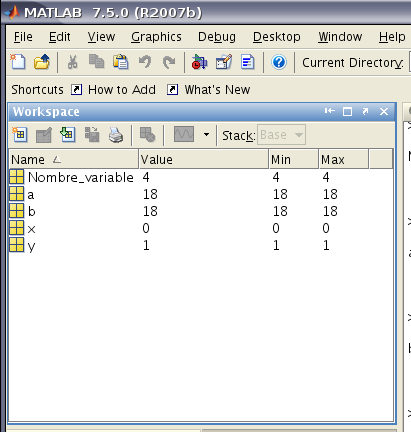
\includegraphics[width=8cm]{wsp1.png}
	\caption{El \emph{Workspace} de Matlab}
	\label{fig:wsp}
\end{figure}

Además del panel que acabamos de describir, es posible listar el contenido de las variables presentes en el \emph{Workspace} empleando dos comandos especiales de Matlab; se trata de los comandos \texttt{who} y \texttt{whos}. El primero de ellos nos devuelve en la ventana de comandos los nombres de las variables contenidas en el \emph{Workspace}. El segundo nos devuelve los nombres de las variables junto con información adicional sobre su contenido, tamaño, etc.
\begin{verbatim}
>> who

Your variables are:

Nombre_variable  b                y                
a                x                

>> whos
  Name                 Size            Bytes  Class     Attributes

  Nombre_variable      1x1                 8  double              
  a                    1x1                 8  double              
  b                    1x1                 8  double              
  x                    1x1                 8  double              
  y                    1x1                 8  double              

>> 
\end{verbatim}

Para eliminar una variable del \emph{Workspace}, se emplea el comando \texttt{clear}.  Si escribimos en la ventana de comandos el comando \texttt{clear}, seguido del nombre de una variables,  Matlab la elimina del \emph{Workspace}. Si escribimos el comando \texttt{clear}, sin añadir nada más, Matlab eliminará TODAS las variables contenidas en el \emph{Workspace}. 

\paragraph*{Formatos de visualización}\index{visualizacion de variables, formatos}\index{Variable! Formato}
Hemos visto en los ejemplos anteriores cómo al realizar una operación en Matlab, se nos muestra el resultado en la ventana de comandos. Además podemos examinar el contenido de cualquier variable contenida en el \emph{workspace} sin más que escribir su nombre en la ventana de comandos y pulsar la tecla \emph{intro}.

Matlab permite elegir la forma en que los resultados se presenta por pantalla. Para ello se emplea el comando \texttt{format}.  La siguiente tabla, resume los formatos más comúnmente empleados.

\begin{table}[h]
\caption{Formatos numéricos más comunes en Matlab}
\begin{tabular}{l l l }
\textbf{Comando} & \textbf{formato} & \textbf{Comentario}\\ \hline
\texttt{format short} & $12.3457$ & coma fija. Cuatro decimales\\
\texttt{format shortE} & $1.2346e+01$ & coma flotante. Cuatro decimales\\
\texttt{format long} & $12.345678901234500$ & coma fija. Quince decimales\\
\texttt{format longE} & $1.234567890123450e+01$ & coma flotante. Quince decimales\\ \hline 
\end{tabular}
\end{table}
\subsection{Vectores y matrices.} \index{Vectores! Definición en matlab} \index{Matrices! Definición en matlab} Una de las característica más interesantes de Matlab, es la posibilidad de crear fácilmente matrices. Se pueden crear de muchas maneras, la más elemental de todas ellas, emplea el operador de asignación $=$, y los símbolos especiales $[$, $]$, el punto y coma $;$ y la coma $,$. Las matrices se crean introduciendo los valores de sus elementos por filas, separados por comas o espacios. Una vez introducidos todos los elementos de una fila, se añade un punto y coma, o se pulsa la tecla \emph{intro}, y se añaden los elementos de la fila siguiente. El siguiente ejemplo muestra como crear una matriz de de dos filas y tres columnas:
\begin{verbatim}
 >> matriz23 =[ 1 3 4 ;3 5 -1]

matriz23 =

     1     3     4
     3     5    -1
\end{verbatim}
o también:
 \begin{verbatim}
  >> matriz23 =[ 1 3 4 
3 5 -1]

matriz23 =

     1     3     4
     3     5    -1
 \end{verbatim}

En el primer caso, se empleado el punto y coma para separar las filas y en el segundo se ha empleado la tecla \emph{intro}.  En ambos se emplea el símbolo $[$ para indicar a Matlab que queremos empezar a construir una matriz, y el símbolo $]$ para indicar a Matlab que hemos terminado de construirla. Una vez construida, Matlab nos devuelve en la ventana de comandos la Matriz completa. Matlab nos permite además emplear cada elemento de una matriz como si se tratase de una variable, es decir, se puede asignar  a los elementos de una matriz un valor numérico, el resultados de una operación o un valor guardado en otra variable:
\begin{verbatim}
>> a=1

a =

          1.00

>> b=2

b =

          2.00

>> mtr=[ a a+b a-b; 1 0.5 cos(0)]

mtr =

          1.00          3.00         -1.00
          1.00          0.50          1.00

>> 
\end{verbatim}

Matlab considera las matrices como la forma básica de sus variables, así para Matlab un escalar es una matriz de una fila por una columna. Un vector \emph{fila} de 3 elementos es una matriz de una fila por tres columnas y un vector \emph{columna} de tres elementos es una matriz de tres filas y una columna.

\paragraph*{Indexación.} \index{Indexación en matlab}Al igual que se hace en álgebra, Matlab es capaz de referirse a un elemento cualquiera de una matriz empleando índices para determinar su posición (fila y columna) dentro de la matriz.
\begin{equation*}
a=
\begin{pmatrix}
a_{11}&a_{12}&a_{13}\\
a_{21}&a_{22}&a_{23}\\
a_{31}&a_{32}&a_{33}
\end{pmatrix}
\end{equation*}

El criterio para referirse a un elemento concreto de una matriz, en Matlab es el mismo: se indica el nombre de la variable que contiene la matriz y a continuación, entre paréntesis y separados por una coma, el índice de su fila y después él de su columna:
 \begin{verbatim}
 >> a=[1 2 3; 4 5 6; 7 8 9]

a =

          1.00          2.00          3.00
          4.00          5.00          6.00
          7.00          8.00          9.00

>> a(1,2)

ans =

          2.00

>> a(2,1)

ans =

          4.00

>> 
 \end{verbatim}
 
Es interesante observar de nuevo cómo Matlab asigna por defecto el valor del elemento buscado a la variable \texttt{ans}. Como ya se ha dicho, es mejor asignar siempre una variable a los resultados, para asegurarnos de que no los perdemos al realizar nuevas operaciones:
\begin{verbatim}
>> a12=a(1,2)

a12 =

          2.00

>> a21=a(2,1)

a21 =

          4.00

>> 
\end{verbatim}
Ahora hemos creado dos variables nuevas que contienen los valores de los elementos $a_{12}$ y $a_{21}$ de la matriz $a$. 

Matlab puede seleccionar dentro de una matriz no solo elementos aislados, sino también submatrices completas. Para ello, emplea un símbolo reservado, el símbolo \emph{dos puntos} $:$. Este símbolo se emplea para recorrer valores desde un valor inicial hasta un valor final, con un incremento o paso fijo. La sintaxis es: \texttt{inicio:paso:fin}, por ejemplo podemos recorrer los números enteros de cero a 8 empleando un paso 2:
\begin{verbatim}
>> 0:2:8

ans =

             0          2.00          4.00          6.00          8.00

>> 
\end{verbatim}

El resultado nos da la lista de los números $0, 2, 4, 6, 8$.
Además, si no indicamos el tamaño del paso,  Matlab tomará por defecto un paso igual a uno. En este caso basta emplear un único símbolo \emph{dos puntos} para separar el valor de inicio del valor final:
 \begin{verbatim}
 >> 1:5

ans =

          1.00          2.00          3.00          4.00          5.00

>>
 \end{verbatim}
 
 Podemos emplear el símbolo \emph{dos puntos},\index{Indexación con el operador :} \index{": Operador de indexación} para obtener submatrices de una matriz dada. Así por ejemplo si construimos una matriz de cuatro filas por cinco columnas:
 \begin{verbatim}
 >> matriz=[1 2 4 5 6
3 5 -6 0 2
4 5 8 9 0
3 3 -1 2 0]

matriz =

          1.00          2.00          4.00          5.00          6.00
          3.00          5.00         -6.00          0.00          2.00
          4.00          5.00          8.00          9.00          0.00
          3.00          3.00         -1.00          2.00          0.00

>> 
 \end{verbatim}
 Podemos obtener el vector formado por los tres últimos elementos de su segunda fila:
 \begin{verbatim}
 >> fil=matriz(2,3:5)

fil =

         -6.00             0          2.00

>> 
 \end{verbatim}

 o la submatriz de tres filas por tres columnas formada por los elementos que ocupan las filas 2 a 4 y las columnas 3 a 5:
\begin{verbatim}
 >> subm=matriz(2:4,3:5)

 subm =

         -6.00          0                2.00
	          8.00          9.00             0  
         -1.00          2.00             0  

 >> 
\end{verbatim}

o el vector columna formado por su segunda columna completa:
\begin{verbatim}
>> matriz(1:4,2)

ans =

          2.00
          5.00
          5.00
          3.00

>> 
\end{verbatim} 

De hecho, si deseamos seleccionar todos los elementos en una fila o una columna, podemos emplear el símbolo \texttt{:} directamente sin indicar principio ni fin,

\begin{verbatim}

>> matriz(:,2)

ans =

          2.00
          5.00
          5.00
          3.00

>> matriz(3,:)
ans =

     4.00     5.00     8.00    9.00    0.00
\end{verbatim}
 
\label{index}A parte de la indexación típica del álgebra de los elementos de una matriz indicando su fila y columna, en Matlab es posible referirse a un  elemento de una matriz empleando un único índice. En este caso, Matlab cuenta los elementos por columnas, de arriba abajo y de izquierda a derecha, 

\begin{equation*}
A=
\begin{pmatrix}
a_1&a_4&a_7\\
a_2&a_5&a_8\\
a_3&a_6&a_9
\end{pmatrix}
\end{equation*}

Así por ejemplo, en una matriz $A$ de $3$ filas y $4$ columnas, 
\begin{verbatim}
>> A=[3 0 -1 0; 2 1 5 7; 1 3 9 8]
A =

     3     0    -1     0
     2     1     5     7
     1     3     9     8
\end{verbatim}
las expresiones,
\begin{verbatim}
>> A(2,3)

ans =
     5
\end{verbatim}
y
\begin{verbatim}
>> A(8)

ans =
     5
\end{verbatim} 
hacen referencia al mismo elemento de la matriz $A$. 

Aunque el concepto de función no se explicará hasta la sección \ref{funciones}, vamos a hacer uso de un par de funciones sencillas relacionadas con el tamaño de una matriz. En primer lugar, tenemos la función \texttt{length}; esta función nos calcula el número total de elementos que contiene un vector, sea este fila o columna.  Así, si tenemos un vector guardado en la variable  \texttt{a}, para saber su longitud escribimos en matlab el nombre de la función seguida del nombre de la variable entre paréntesis \texttt{length(a)},

\begin{verbatim}
>> a = [ 1 -2 0 6 8]
a =

     1    -2     0     6     8
>> length(a)

ans =

     5

>> 
\end{verbatim} 

La segunda función es la función \texttt{size}, esta función permite obtener el número de filas y columnas de una matriz o vector. \texttt{size} nos da como resultado de aplicarlo a una matriz un vector cuyo primer elemento es el número de filas de la matriz, y cuyo segundo elemento el número de columnas,

\begin{verbatim}
>> A = [1 3 4 -5; 2 3 0 -2; -2 1 7 7]
A =

     1     3     4    -5
     2     3     0    -2
    -2     1     7     7

>> size(A)

ans =

     3     4
\end{verbatim}  


\subsection{Estructuras y células}\index{Estructuras}\index{Células (cells)}
Se trata de dos tipos de variables especiales. Ambas comparten la propiedad de poder combinar dentro de sí variables de distintos tipos.

\paragraph*{Estructuras.} Una estructura es una variable que guarda la información divida en campos. Por ejemplo, si escribimos en la ventana de matlab,

\begin{verbatim}
>> est.nombre='Ana'
est = 
    nombre: 'Ana'
>> est.edad=25
est = 
    nombre: 'Ana'
      edad: 25
\end{verbatim}

obtenemos una estructura con dos campos, el primero de ellos es el campo \texttt{nombre}, y guarda dentro una cadena de caractéres \texttt{'Ana'}, el segundo es el campo \texttt{edad} y guarda dentro el valor \texttt{25}. La estructura que acabamos de definir es una sola variable llamada \texttt{est} y podemos aplicar cualquier comando de matlab cuyo resultado no dependa del contenido específico de la variable. Podemos copiarla en otra estructura,

\begin{verbatim}
>> est2=est
est2 = 
    nombre: 'ana'
      edad: 25
\end{verbatim}
podemos borrarla,

\begin{verbatim}
>> clear est
>> who
Your variables are:
est2  
>> 
\end{verbatim}

No podemos realizar sobre ella, como un todo, operaciones aritméticas o relacionales, pero sí sobre sus campos,

\begin{verbatim}
>> x=est.edad+12
x =
    37
\end{verbatim} 

El número de campos de una estructura puede aumentarse añadiendo a su nombre, el nombre del nuevo campo separado por un punto y asignando un valor o una variable a dicho campo.

\begin{verbatim}
>> est.campo_nuevo=[1 2;3 4; 6 7]
est = 
         nombre: 'ana'
           edad: 25
    campo_nuevo: [3x2 double]
    >> y=[1 2 3]
y =
     1     2     3
>> est.campo_nuevo2=y
est = 
          nombre: 'ana'
            edad: 25
     campo_nuevo: [3x2 double]
    campo_nuevo2: [1 2 3]
\end{verbatim}
 
 Podemos tambien eliminar campos de una estructura mediante el comando \texttt{rmfield},
 
 \begin{verbatim}
 >> est=rmfield(est,'edad')
est = 
          nombre: 'ana'
     campo_nuevo: [3x2 double]
    campo_nuevo2: [1 2 3]
 \end{verbatim}
 
Por último, una estructura nos permite definir y utilizar varios niveles de campos. Para ello, basta ir definiendo los nombres de los campos de un nivel separados por un punto del nombre del nivel anterior, 

\begin{verbatim}
>> multinivel.datos_personales.nombre='Ana'
multinivel = 
    datos_personales: [1x1 struct]
>> multinivel.datos_personales.primer_apellido='Jiménez'
multinivel = 
    datos_personales: [1x1 struct]
>> multinivel.datos_personales.segundo_apellido='Lasarte'
multinivel = 
    datos_personales: [1x1 struct]
>> multinivel.domicilio.calle='Ponzano'
multinivel = 
    datos_personales: [1x1 struct]
           domicilio: [1x1 struct]
>> multinivel.domicilio.numero=724
multinivel = 
    datos_personales: [1x1 struct]
           domicilio: [1x1 struct]
>> multinivel.valor=[3 4 5; 3.5 2 3]
multinivel = 
    datos_personales: [1x1 struct]
           domicilio: [1x1 struct]
               valor: [2x3 double]
\end{verbatim}

La información se encuentra ahora estructurada en niveles. Así por ejemplo,

\begin{verbatim}
>> multinivel.domicilio
ans = 
     calle: 'Ponzano'
    numero: 724
\end{verbatim}

Me devuelve el contenido del campo \texttt{domicilio} que es a su vez una estructura formada por dos campos  \texttt{calle} y  \texttt{numero}. La información queda estructurada en niveles que pueden ramificarse tanto como se desee. Para obtener la información contenida al final de una rama, es preciso indicar todos los campos que se atraviesan hasta llegar a ella,

\begin{verbatim}
>> multinivel.datos_personales.segundo_apellido
ans =
Lasarte
\end{verbatim}

Matlab tiene definidas funciones propias para conseguir un manejo eficiente de las estructuras. A parte de la función \texttt{rmfield} de la que hemos hablado anteriormente, cabe destacar la función \texttt{struct} que permite crear directamente una estructura. Su sintaxis es,

\begin{verbatim}
 s= struct('field1', values1, 'field2', values2, ...)
\end{verbatim}

donde \texttt{s} representa el nombre de la estructura, \texttt{field1},\texttt{field2}, etc son los nombres correspondientes a cada campo, introducidos entre comillas, y \texttt{values1}, etc los valores contendidos en cada campo. Para un conocimiento más profundo del uso de las estructuras se aconseja consultar la ayuda de Matlab.

\paragraph*{Células.} Las células, \emph{cells} en Matlab, son objetos que almacenan datos de diversos tipos en una misma variable. A diferencia de las estructuras, las células no expanden un árbol de campos sino que guardan cada dato en una "celda".  Para referirse a una celda concreta, empleamos un índice, de modo análogo a como hacemos con un vector.  Para construir una célula, procedemos de modo análogo a como hacemos con un vector, pero en lugar de emplear corchetes como delimitadores, empleamos llaves. Así, por ejemplo,

 \begin{verbatim}
 >> a={[1 2 3; 4 5 6; 7 8 9],'cadena', -45;'pepe', [1 2 3], 'cadena2'}
a = 
    [3x3 double]    'cadena'        [    -45]
    'pepe'          [1x3 double]    'cadena2'
 \end{verbatim}

Hemos creado una célula \texttt{a}, cuyos elementos son, una matriz $3\times 3$, la cadena de caracteres \texttt{cadena}, el número $-45$, otra cadena de caracteres \texttt{pepe}, el vector $[1,2,3]$ y una última cadena de caracteres \texttt{cadena2}.

Los elementos separados por espacios o por comas simples, pertenecen a la misma fila dentro de la célula. Los elementos pertenecientes a distintas filas están separados por un punto y coma.  Podemos obtener el tamaño de la célula ---su número de filas y columnas--- empleando el comando \texttt{size} , igual que hicimos para el caso de vectores o matrices,

\begin{verbatim}
>> size(a)
ans =
     2     3
\end{verbatim}

Y podemos referirnos a una celda cualquiera de la célula, y obtener su contenido indicando entre llaves la fila y la columna a la que pertenece. Así por ejemplo, para obtener el vector $[1,2,3]$ de la célula \texttt{a} del ejemplo anterior hacemos,
\begin{verbatim}
>> vector=a{2,2}
vector =
     1     2     3
\end{verbatim}

Las celdas, de modo análogo a como sucedía con las estructuras, nos permiten agrupar datos de distinto tipo empleando una sola variable. Además, el hecho de que los datos ester ordenados por celdas en filas y columna, hace sencillo que se puede acceder a ellos.
 
\section{Entrada y salida de Datos}\index{Datos! Entrada y Salida}
Matlab posee una amplia colección de métodos para importar datos desde y exportar datos a un fichero. A continuación describimos algunos de los más usuales.

\subsection{Exportar e importar datos en Matlab} \label{fpf}

\paragraph*{Datos en formato propio de Matlab}
Matlab posee un formato de archivo propio para manejar sus datos. Los archivos de datos propios de Matlab, emplean la extensión \texttt{.mat}.


Si tenemos un conjunto de variables en el \emph{workspace}, podemos guardarlas en un fichero empleando el comando \texttt{save}, seguido del nombre del fichero donde queremos guardarlos. No es preciso incluir la extensión \texttt{.mat}, Matlab la añade automáticamente:
\begin{verbatim}
>> save datos
\end{verbatim}
Matlab creará en el directorio de trabajo un nuevo fichero \texttt{datos.mat} en el que quedarán guardadas todas las variables contenidas en el \emph{workspace}.  Los ficheros \texttt{.mat} generados por Matlab están escritos en binario. No se puede examinar su contenido empleando un editor de textos. Matlab almacena toda la información necesaria ---nombre de las variables, tipo, etc--- para poder volver a reconstruir las variables en el \emph{workspace} tal y como estaban cuando se generó el archivo.


Es posible guardar tan solo algunas de las variables contenidas en el \emph{workspace} en lugar de guardarlas todas. Para ello, basta añadir al comando \texttt{save}, detrás del nombre del archivo, el nombre de las variables que se desean guardar, separadas entre sí por un espacio
\begin{verbatim}
>>save datos1 A  matriz_1 B 
\end{verbatim}
La instrucción anterior guarda en un archivo ---llamado datos1.mat--- las variables \texttt{A}, \texttt{matriz1} y \texttt{B}.


Los datos contenidos en cualquier fichero \texttt{.mat} generado con el comando \texttt{save} de Matlab, pueden volver a cargarse en el \emph{workspace} empleando el comando \texttt{load}, seguido del nombre del fichero cuyos datos se desean cargar:
\begin{verbatim}
load datos.mat
\end{verbatim}
 carga en el \emph{workspace} las variables contenidas en el fichero \texttt{datos.mat}, la extensión del fichero puede omitirse al emplear la función \texttt{load}. Si conocemos los nombres de las variables contenidas en un archivo \texttt{.mat}, podemos cargar en Matlab solo una o varias de las variables contenidas en el archivo, escribiendo sus nombres, separados por espacios, detrás del nombre del archivo: 
\begin{verbatim}
>>load datos A G matriz1
\end{verbatim}
 cargará tan solo las variables \texttt{A}, \texttt{G} y \texttt{matriz1}, de entre las que contenga el ficheros \texttt{datos.mat}

\paragraph*{Datos en Formato ASCII} \index{Datos!Formato ASCII}\index{ASCII, Formato de datos}e puede emplear también el comando \texttt{save} para exportar datos en formato ASCII. Pare ello es preciso añadir al comando modificadores,
\begin{verbatim}
>>save datos.txt A -ASCII
\end{verbatim}

Este comando guardará la variable \texttt{A} en el fichero \texttt{datos.txt}. Matlab no añade ninguna extensión por defecto al nombre del fichero cuando empleamos el comando \texttt{save} con el modificador \texttt{-ASCII}. En este caso, hemos añadido explícitamente la extensión \texttt{.txt}, esto facilita que el archivo resultante se pueda examinar luego empleando un sencillo editor de texto o una hoja de cálculo.


Cuando se exportan datos desde Matlab en formato ASCII, Matlab guarda tan solo los valores numéricos contenidos en las variables, pero no los nombres de éstas. Por otro lado, guarda tan solo ocho dígitos, por lo que habitualmente se pierde precisión. Es posible guardar  datos en formato ASCII, conservando toda la precisión, si añadimos al comando \texttt{save} el modificador \texttt{-DOUBLE}, 
\begin{verbatim}
>>save nombre_Archivo matriz_1, matriz2, ... -ASCII -DOUBLE
\end{verbatim}


Supongamos que en \emph{workspace} tenemos guardada la siguiente matriz,

\begin{equation*}
a=
\begin{pmatrix}
1.300236890000000e+000&3.456983000000000e+000&4.321678000000000e+006\\
4.000230000000000e+003&1.245677000000000e+001&1.231565670000000e+002
\end{pmatrix}
\end{equation*}
Si ejecutamos en Matlab, 
\begin{verbatim}
>>save datos.txt a -ASCII
\end{verbatim}

El fichero resultante tendrá el aspecto siguiente,
\begin{verbatim}
   1.3002369e+00   3.4569830e+00   4.3216780e+05
   4.0002300e+03   1.2456770e+01   1.2315657e+02
\end{verbatim}

es decir, los elementos de una misma fila de la matriz \texttt{a} se guardan en una fila separados por espacios, las filas de la matriz se separan empleando retornos de carro ---cada una ocupa una línea nueva--- y los valores cuyos dígitos significativos exceden de 8 se han truncado, redondeando el último dígito representado. Este último es el caso de los elementos $a_{11}$ y $a_{33}$ de la matriz del ejemplo.

Cuando se guardan varias variables o todo el \emph{workspace} en un mismo fichero con formato ASCII, es preciso tener en cuenta que Matlab se limitará a guardar los contenidos de las variables, uno debajo de otro, en el orden en que las escribamos detrás del comando \texttt{save} (en el caso de que guardemos todas las variables del \emph{workspace} las guardará una debajo de otra por orden alfabético), por lo que resulta difícil distinguir las variables originales.
Así por ejemplo, si tenemos en el \emph{workspace} las variables,
 \begin{equation*}
 A=
 \begin{pmatrix}
3&5\\
2&1\\
8&0
\end{pmatrix}
a=
\begin{pmatrix}
1&3&4\\
4&5.6&2\\
3&0&1
\end{pmatrix}
c=
\begin{pmatrix}
3&2
\end{pmatrix}
\end{equation*}
La orden,
\begin{verbatim}
>>save datos.txt c a A -ASCII
\end{verbatim}

produce el un archivo con el siguiente contenido,
\begin{verbatim}
   3.0000000e+00   2.0000000e+00
   1.0000000e+00   3.0000000e+00   4.0000000e+00
   4.0000000e+00   5.6000000e+00   2.0000000e+00
   3.0000000e+00   0.0000000e+00   1.0000000e+00
   3.0000000e+00   5.0000000e+00
   2.0000000e+00   1.0000000e+00
   8.0000000e+00   0.0000000e+00
\end{verbatim}

El comando \texttt{load}, presenta algunas limitaciones para cargar datos contenidos en un fichero ASCII. Solo funciona correctamente si el contenido del fichero puede cargarse en una única matriz, es decir, cada fila de datos en el fichero debe contener el mismo número de datos. Así, en el ejemplo anterior, los datos guardados en el fichero \texttt{datos.txt}, no pueden volver a cargarse en Matlab usando el comando load.

Para el caso de un fichero cuyos contenido pueda adaptarse a una matriz, el comando load carga todos los datos en una única matriz a la que asigna el nombre del fichero sin extensión.

\paragraph*{Lectura y escritura de datos con formato} \index{Datos!Lectura y escritura}

Matlab puede también escribir y leer datos, empleando formatos y procedimientos similares a los de el lenguaje C. Para ello, es preciso emplear varios comandos\footnote{Lo que se ofrece a continuación es solo un resumen del uso de los comandos y formatos más frecuentes. Para obtener una información completa, consultar la ayuda de Matlab.}:

En primer lugar es preciso crear ---o si ya existe abrir--- el archivo en que se quiere guardar o del que se quieren leer los datos. En ambos casos se emplea para ello el comando \texttt{fopen}. La sintaxis de este comando es de la forma,
\begin{verbatim}
fid=fopen(nombre de fichero, permisos)
\end{verbatim} 
El nombre del fichero debe ser una cadena de caracteres, es decir, debe ir escrito entre apóstrofos. Hay al menos ocho tipos de permisos distintos. Aquí describiremos tan solo tres de ellos, \texttt{'w'} ---\emph{write}--- abre o crea un archivo con permiso de escritura. Si el archivo ya existía su contenido anterior se sobreescribe. Si se quiere añadir datos a un archivo sin perder su contenido se emplea el permiso \texttt{'a'} ---\emph{append}--- los nuevos datos introducidos se escriben al final del fichero, a continuación de los ya existentes. \texttt{'r'} ---\emph{read}--- permiso de lectura, es la opción por defecto, permite leer el contenido de un archivo. Cuando se trabaja en el sistema operativo \emph{Windows}, es común emplear los permisos en la forma \texttt{'wt'} y \texttt{'rt'}, de este modo, los archivos se manejan en el denominado formato 'texto'. La variable \texttt{fid}, es un identificador del fichero abierto y es también la forma de referirnos a él ---en un programa, o en la línea de comandos--- mientras permanece abierto.

Supongamos que hemos abierto ---o creado--- un archivo para escribir en él, datos contenidos en el \emph{workspace}, 
\begin{verbatim}
fichero1=fopen('mi_fichero','wt') 
\end{verbatim}

Para escribir en él emplearemos el comando fprintf. La sintaxis de este comando necesita un identificador de archivo --en nuestro caso sería fichero1--, un descriptor del formato con el que se desean guardar los datos y el nombre de la variable que se desea guardar.
\begin{verbatim}
control=fprintf(fichero1,formato,nombre_de_variable,...)
\end{verbatim} 
Los descriptores de formato se escriben entre apóstrofos. Empiezan siembre con el carácter \texttt{\%}, seguido de un número con formato \emph{e.d}. Donde \emph{e} recibe el nombre de anchura de campo  y \emph{d} recibe el nombre de precisión. Por último se añade un carácter, conocido como carácter de conversión, que permite ajustar el formato numérico de los datos. Los más usuales son: \texttt{f} ---notación de punto fijo---, \texttt{e} ---notación exponencial--- y \texttt{g} ---la notación que resulte más compacta de las dos anteriores---.  La anchura de campo representa en número mínimo de caracteres que se emplearán para representar el número.  La precisión depende del carácter de conversión; para \texttt{f} y  \texttt{e}, representa el número de dígitos  a la derecha del punto decimal, para  \texttt{g} el número de dígitos significativos.

Aquí hemos incluido solo los caracteres de conversión más usuales para el caso de datos numéricos. Cabe añadir que para el caso de una cadena de caracteres se emplea como carácter de conversión la letra $s$.  Por ejemplo:

\begin{verbatim}
>>A='mi cadena de caracteres'
>>num=fprinf(fid,'%s', A)
\end{verbatim}
Escribe  el texto contenido en el vector \texttt{A} en el archivo indicado por \texttt{fid}.
 
Matlab, almacena los datos consecutivamente uno detrás de otro. Si se trata de matrices, los va leyendo por columnas y una variable tras otra en el orden en que se hayan introducido al llamar a la función \texttt{fprintf}. Para separar entre sí los datos se puede añadir a los descriptores de formatos, espacios y también caracteres de escape como Retornos de carro \texttt{\textbackslash r}, indicadores de salto de línea \texttt{\textbackslash n} o tabuladores \texttt{\textbackslash t}, entre otros.

Por ejemplo, supongamos que tenemos en Matlab las siguiente matrices

 \begin{equation*}
 A=
 \begin{pmatrix}
3.25&5.22\\
23.1&130.5\\
8&0
\end{pmatrix}
a=
\begin{pmatrix}
1.2345&3.0879&4234.2\\
40&5000.6&223\\
3&0&1
\end{pmatrix}
c=
\begin{pmatrix}
30&2
\end{pmatrix}
\end{equation*}

Si empleamos,
\begin{verbatim}
>>num=fprinf(fid,'%2.1f', A, a, c)
\end{verbatim}

Los datos se guardarán en el archivo indicado por \texttt{fid} en la siguiente forma:
\begin{verbatim}
3.223.18.05.2130.50.01.240.03.03.15000.60.04234.2223.01.030.02.0
\end{verbatim}

Guardados en este formato resulta bastante difícil reconocerlos. Si probamos,
\begin{verbatim}
>>num=fprinf(fid,'%2.1f ', A, a, c)
\end{verbatim}

El resultado sería,
\begin{verbatim}
3.2 23.1 8.0 5.2 130.5 0.0 1.2 40.0 3.0 3.1 5000.6 0.0 4234.2 223.0 1.0 30.0 2.0
\end{verbatim}

El formato es de punto fijo y los datos aparecen separados por un espacio ---nótese que en el descriptor de formato se ha incluido un espacio entre la f y el apóstrofo---. Los datos de las tres matrices aparecen uno detrás de otro, y se han ido escribiendo en el archivo por columnas

Si cambiamos de nuevo el descriptor de formato,
\begin{verbatim}
>>num=fprinf(fid,'%2.3g\n', A, a c)
\end{verbatim}
obtendremos,
\begin{verbatim}
3.25
23.1
 8
5.22
130
 0
1.23
40
 3
3.09
5e+03
 0
4.23e+03
223
 1
30
\end{verbatim}
Matlab elige el formato más compacto para cada dato, y guarda cada dato en una fila nueva, debido al término \texttt{\textbackslash n} introducido al final del descriptor.

Por último indicar que es posible emplear varios descriptores consecutivos, en cuyo caso, Matlab los aplica a cada dato consecutivamente, cuando ha terminado con la lista de descriptores, comienza de nuevo por el principio.

Por ejemplo, 

\begin{verbatim}
>>num=fprinf(fid,'%2.3g %2.3g %2.3g\n', a)
\end{verbatim}
Guarda los datos contenidos en \texttt{a} como,
\begin{verbatim}
1.23 40 3.09
5e+03 4.23e+03 223
\end{verbatim}

Es decir cada tres datos cambia a una línea nueva. Por supuesto, podríamos hacer que los datos se guardaran con un formato distinto en cada caso,
\begin{verbatim}
>>num=fprinf(fid,'%2.3g %3f %2.3f\n', a)

1.23 40.000000 3.088
5e+03 4234.200000 223.000
\end{verbatim}

Por último indicar, que si se emplea el comando \texttt{fprintf} sin emplear un  identificador de archivo o empleando como identificador el valor $1$. Matlab escribe el resultado directamente en la ventana de comandos con el formato deseado.

Por ejemplo, 
\begin{verbatim}
>>B = [8.8  7.7; 8800  7700];
>>fprintf(1, 'X is %6.2f metros o %8.3f mm\n', 9.9, 9900, B)
\end{verbatim}
Mostrará en la ventana de comandos las siguientes líneas:
\begin{verbatim}
X is 9.90 metros o 9900.000 mm
X is 8.80 metros o 8800.000 mm
X is 7.70 metros o 7700.000 mm
\end{verbatim}


Para cargar archivos desde un fichero que contiene datos en binario, se emplea el comando \texttt{fscanf}. Su uso es similar al de \texttt{fprintf}, pero ahora los datos pasarán desde el fichero donde están guardados a una matriz.

\begin{verbatim}
>>A=fscanf(pid,'%f')
\end{verbatim}

El comando \texttt{fscanf}, admite como parámetros  el número máximo de datos que se leerán del fichero,
\begin{verbatim}
a=fscanf(fid,'%5.2f',M)
\end{verbatim}
Lee como máximo M datos del fichero y los guarda en un vector \texttt{a}. Es posible dar a los datos formato de matriz, mediante dos parámetros (fila y columna),
\begin{verbatim}
a=fscanf(fid,'%5.2f',[M,N])
\end{verbatim}
Ahora creará una matriz \texttt{a} de M filas por N columnas. Matlab irá cogiendo los datos del fichero, por columnas hasta rellenar la matriz.

Es posible dar al segundo parámetro el valor \texttt{inf}. De este modo, Matlab creará una matriz de \texttt{M} filas y el número de columnas necesario para cargar todos los datos del fichero. (Si faltan elementos para completar la matriz resultante, Matlab rellena los huecos con ceros.)
Por último, una vez que se han escrito o leído datos en el fichero es preciso cerrarlo correctamente empleando el comando \texttt{fclose}, la sintaxis de este comando solo precisa que se incluya el identificador del fichero que se quiere cerrar,
\begin{verbatim}
>>fclose(fid)
\end{verbatim}

\paragraph*{Herramienta de importación de datos}\index{Datos! Importación}
Matlab posee una herramienta especial para importar datos. Con ella, es posible cargar en Matlab datos de muy diverso tipo, no sólo numéricos sino también imágenes, sonido, etc. Una de las ventajas de esta herramienta es que reconoce directamente ---entre otros--- los archivos creados por las hojas de cálculo.
\begin{figure}[h]
	\centering
		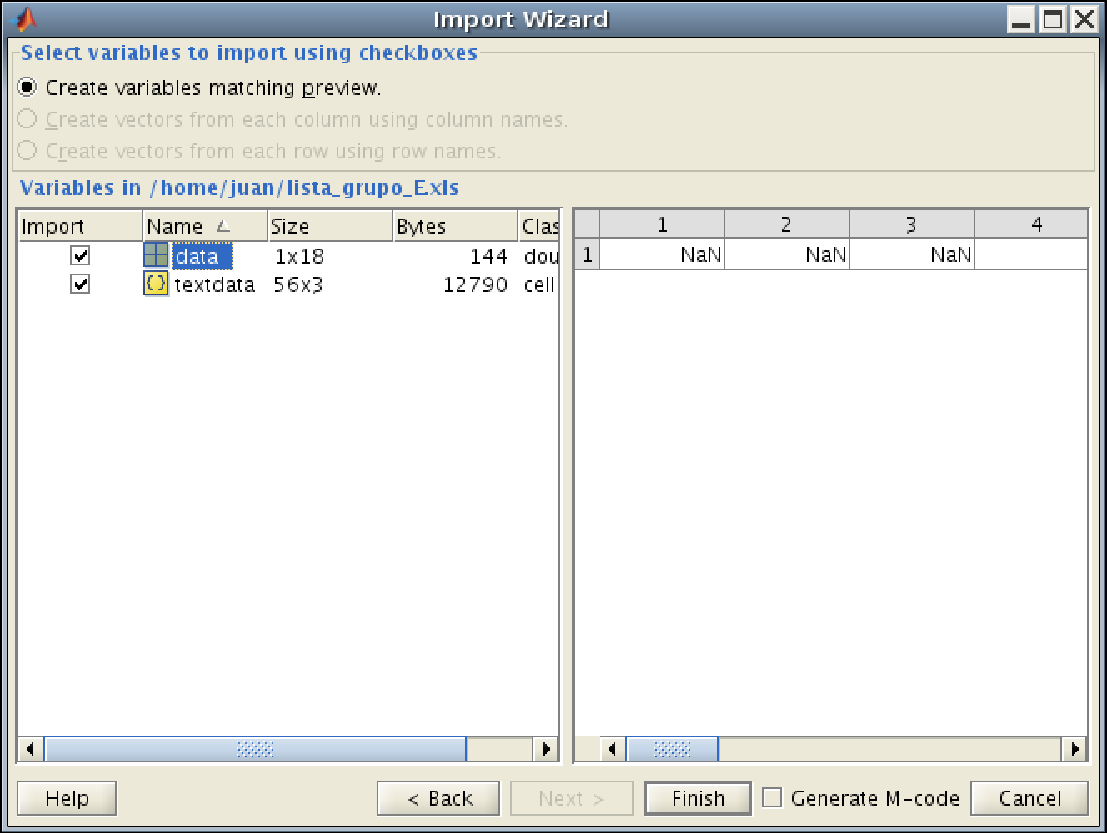
\includegraphics[width=10cm]{Wizard.pdf}
	\caption{Aspecto de la herramienta de importación de datos}
	\label{fig:wizard}
\end{figure}

Para abrir en Matlab la herramienta de importación, basta seleccionar en la pestaña \emph{file} la opción \emph{Import Data}. Matlab abre entonces una ventana que nos permite navegar por el árbol de directorio y seleccionar el archivo del que deseamos importar los datos. Una vez seleccionado, Matlab abre la ventana mostrada en la imagen \ref{fig:wizard}. 
Se trata de un programa especial ---\emph{import wizard}--- que sirve para guiar al usuario en el proceso de cargar las variables contenidas en el fichero en el \emph{workspace} de Matlab.

\section{Operaciones aritméticas, relacionales y lógicas}\index{Operaciones}

\subsection{Operaciones aritméticas}\index{Operaciones!Aritméticas}
 Una vez que sabemos como crear o importar variables en Matlab, vamos a ver como podemos realizar operaciones aritméticas elementales con ellas. La sintaxis es muy sencilla, y podemos sintetizarla de la siguiente manera:
\begin{equation*}
resultado=operando_1 operador_1 operando_2 operador_2 operando_3 \cdots operando_{n-1} operador_n
\end{equation*}
Es decir basta concatenar los operadores con los operandos y definir una variable en la que guardar el resultado. Por ejemplo,
\begin{verbatim}
>>x=1; y=2; z=3; q=x+y+z
>>z=6
\end{verbatim}
En este caso los operandos son las variables \texttt{x}, \texttt{y}, \texttt{z}, el operador, que se repite dos veces es el símbolo \texttt{+} que representa la operación suma y \texttt{q} es la variable en la que se guarda el resultado, en este caso, de la suma de las tres variables anteriores.

Los operadores aritméticos disponibles en Matlab cubren las operaciones aritméticas habituales, pero hay que recordar que Matlab considera sus variables como matrices. Por lo tanto, las operaciones definidas Matlab las considera por de defecto operaciones entre matrices. La tabla \ref{tabop} contiene los operadores definidos en  Matlab.

\begin{table}[h]
\caption{Operadores aritméticos definidos en Matlab}
\label{tabop}
\centering
\begin{tabular}{cccc}
operación&símbolo&ejemplo&notas\\
\hline
suma&\texttt{+}&\texttt{r=a+b}&suma matricial\\
\hline
diferencia&\texttt{-}\\
\hline
producto&\texttt{*}&\texttt{r=a*b}&producto matricial\\
producto&\texttt{.*}&\texttt{r=a.*b}&producto por elementos\\
\hline
división&\texttt{/}&\texttt{d=a/b}& división: $a\cdot b^{-1}$\\
división& \texttt{./}& \texttt{d=a./b}& división por elementos\\
división& \texttt{\textbackslash}& \texttt{d=a\textbackslash b}& división por la izquierda: $a^{-1}\cdot b$\\
\hline
potenciación&\texttt{\^}&\texttt{y=a \^\ b}&potencia de una matriz \\
potenciación&\texttt{.\^}&\texttt{y=a .\^\ b}&potencia elemento a elemento\\
\hline
trasposición&\texttt{'}&\texttt{y=a'}&matriz traspuesta\\
\hline
\hline
\end{tabular}
\end{table}

A continuación, veremos algunos ejemplos de manejo de operaciones básicas. Hemos visto ya el manejo de la suma. Si se trata de matrices en vez de números,

\begin{verbatim}
>> A=[1 2 3; 4 5 6; 7 8 9]

A =

     1     2     3
     4     5     6
     7     8     9

>> B=[4 5 6; 2 0 3; -1 2 4]

B =

     4     5     6
     2     0     3
    -1     2     4

>> C=A+B

C =

     5     7     9
     6     5     9
     6    10    13
\end{verbatim}
 Por supuesto, hay que respetar las condiciones en que es posible realizar una operación aritmética entre matrices. La operación,
 
\begin{verbatim}
>> A=[1 2 3; 4 5 6; 7 8 9]

A =

     1     2     3
     4     5     6
     7     8     9

>> B=[4 5 6; 2 0 3]

B =

     4     5     6
     2     0     3

>> C=A+B
Error using  + 
Matrix dimensions must agree.
\end{verbatim}
da un error porque solo es posible sumar matrices del mismo tamaño.\footnote{Ver las definiciones de las operaciones matriciales en el capitulo \ref{opmatr}.}

En el caso del producto, Matlab define dos operaciones distintas. La primera es el producto matricial normal, 
\begin{verbatim}
>> A=[1 2 3; 4 5 6; 7 8 9]
A =

     1     2     3
     4     5     6
     7     8     9

>> B=[3 4; -2 1; 6 7]
B =

     3     4
    -2     1
     6     7

>> P=A*B
P =

    17    27
    38    63
    59    99
\end{verbatim}

El segundo producto, no es propiamente una operación aritmética definida sobre matrices. Se trata de un producto realizado elemento a elemento. Para ello los dos factores deben ser matrices del mismo tamaño. El resultado es una nueva matriz de igual tamaño que las iniciales en la que cada elemento es el producto de los elementos que ocupaban la misma posición en las matrices factores,

\begin{verbatim}
>> A = [1 2 3; 4 5 6]

A =

     1     2     3
     4     5     6

>> B = [2 3 4; 1 2 3]

B =

     2     3     4
     1     2     3

>> C =A.*B

C =

     2     6    12
     4    10    18
\end{verbatim}

En general, cualquier operador al que se antepone un punto \texttt{.* ./ .\^} indica una operación realizada elemento a elemento.

La división no está definida para matrices. Sin embargo, en Matlab hay definidas tres divisiones. La primera, emplea el símbolo clásico de división, para simples números realiza la división normal. Para matrices, la operación es equivalente a multiplicar el primer operando por la matriz inversa del segundo. $A/B \equiv A\cdot B^{-1}$. Las siguientes tres operaciones son equivalentes en Matlab, aunque desde el punto de vista del  cálculo empleado para obtener el resultado, son numéricamente distintas,

\begin{verbatim}
>> A=[1 2 3; 4 5 6; 7 8 9]
A =

     1     2     3
     4     5     6
     7     8     9

>> B=[2 0 1; 3 2 -1; -2 0 2]
B =

     2     0     1
     3     2    -1
    -2     0     2

>> C=A/B
C =

    0.6667    1.0000    1.6667
    1.6667    2.5000    3.4167
    2.6667    4.0000    5.1667

>> C=A*inv(B)
C =

    0.6667    1.0000    1.6667
    1.6667    2.5000    3.4167
    2.6667    4.0000    5.1667

>> C=A*B^-1
C =

    0.6667    1.0000    1.6667
    1.6667    2.5000    3.4167
    2.6667    4.0000    5.1667
\end{verbatim}  

En el primer caso se ha empleado la división, en el segundo se a multiplicado la matriz \texttt{A} por la inversa de \texttt{B}, calculándola mediante la función de Matlab \texttt{inv}, y en el tercer caso se ha multiplicado la matriz \texttt{A} por \texttt{B} elevado a $-1$.

La división elemento a elemento, funciona de modo análogo a como lo hace la multiplicación elemento a elemento. 

La división por la izquierda, representada mediante el símbolo \texttt{\textbackslash} es equivalente a multiplicar la inversa del primer operando por el segundo,  $A \backslash B \equiv A^{-1} \cdot B$.
\begin{verbatim}

>> A=[1 2 3; 4 5 6; 3 -4 9]
A =

     1     2     3
     4     5     6
     3    -4     9

>> B=[2 0 1; 3 2 -1; -2 0 2]
B =

     2     0     1
     3     2    -1
    -2     0     2

>> C=A\B
C =

   -0.9000    1.0000   -1.5500
    0.8000         0    0.1000
    0.4333   -0.3333    0.7833

>> C=A^-1*B
C =

   -0.9000    1.0000   -1.5500
    0.8000    0.0000    0.1000
    0.4333   -0.3333    0.7833

>> C=inv(A)*B
C =

   -0.9000    1.0000   -1.5500
    0.8000    0.0000    0.1000
    0.4333   -0.3333    0.7833
\end{verbatim}

Uno de los usos típicos de la división por la izquierda, es la resolución de sistema de ecuaciones lineales (ver tema \ref{sistemas}). Por ejemplo, dado el sistema de ecuaciones,

\begin{equation*}
\left. \begin{aligned}
3&x_1+2x_2-4x_3=3\\
2&x_1+ \ \ x_2+3x_3=-3\\
&x_1+3x_2+2x_3=7
\end{aligned}\right\} \Rightarrow	\overbrace{\begin{pmatrix}
3& 2& -4\\
2& 1& \ 3\\
1& 3& \ 2
\end{pmatrix}}^A \cdot \overbrace{\begin{pmatrix}
x_1\\
x_2\\
x_3
\end{pmatrix}}^x=\overbrace{\begin{pmatrix}
 \ 3\\
-3\\
-7
\end{pmatrix}}^b
\end{equation*}

Podemos resolverlo en Matlab con una sencilla división por la izquierda,

\begin{verbatim}
>> A=[3 2 -4; 2 1 3; 1 3 2]

A =

     3     2    -4
     2     1     3
     1     3     2

>> b=[3;-3;-7]
b =

     3
    -3
    -7

>> x=A\b
x =

     1
    -2
    -1
\end{verbatim}
Aunque la potenciación en Matlab tiene más usos, solo consideraremos el caso de una matriz elevada a un número. El resultado será multiplicar la matriz por si misma tantas veces como indique el exponente, $A^3=A\cdot A \cdot A$,
\begin{verbatim}
>> A=[3 0 -1; 2 1 0; 1 3 2]

A =

     3     0    -1
     2     1     0
     1     3     2

>> A^3

ans =

    13   -18   -18
    24    -5   -12
    54    18    -5

>> A*A*A

ans =

    13   -18   -18
    24    -5   -12
    54    18    -5

\end{verbatim}

La potenciación elemento a elemento eleva cada elemento de la matriz al valor que indique el exponente,

\begin{verbatim}
>> B = [1 2 3;3 4 5]

B =

     1     2     3
     3     4     5

>> B.^2

ans =

     1     4     9
     9    16    25

\end{verbatim}
Trasponer una matriz es obtener una nueva matriz intercambiando las filas con las columnas de la matriz original, (ver capítulo \ref{opmatr}). Así por ejemplo,
\begin{verbatim}
>> A=[3 0 -1 0; 2 1 0 0]

A =
     3     0    -1     0
     2     1     0     0

>> B=A'
B =

     3     2
     0     1
    -1     0
     0     0
\end{verbatim}
Las matrices \texttt{A} y \texttt{B} son traspuestas entre sí.

\subsection{Precedencia de los operadores aritméticos}{Operadores!Precedencia}
Combinando operadores aritméticos, es posible elaborar expresiones complejas. Por ejemplo,
\begin{verbatim}
R=5*3-6/3+2^3+2-4
\end{verbatim}
La pregunta que surge inmediatamente es en qué orden realiza Matlab las operaciones indicadas. Para evitar ambigüedades, Matlab ---como todos los lenguajes de programación--- establece un orden de precedencia, que permite saber exactamente en qué orden se realizan las operaciones. En Matlab el orden de precedencia es:
\begin{enumerate}
\item En primer lugar se calculan las potencias.
\item A continuación los productos y las divisiones, que tienen el mismo grado de precedencia.
\item Por último, se realizan las sumas y las restas. 
\end{enumerate} 

Por tanto, en el ejemplo que acabamos de mostrar, Matlab calcularía primero,
\begin{verbatim}
2^3=8
\end{verbatim}
a continuación el producto y la división
\begin{verbatim}
5*3=15
6/3=2
\end{verbatim}
Por último sumaría todos los resultados intermedios, y guardaría el resultado en la variable \texttt{R}
\begin{verbatim}
15-2+8-4=17
R=17
\end{verbatim}

\paragraph{Uso de paréntesis para alterar el orden de precedencia.}
Cuando necesitamos escribir una expresión complicada, en muchos casos el necesario alterar el orden de precedencia. Para hacerlo, se emplean paréntesis. Sus reglas de uso son básicamente dos:
\begin{itemize}
\item La expresiones entre paréntesis tienen precedencia sobre cualquier otra operación.
\item Cuando se emplean paréntesis anidados (unos dentro de otros) los resultados siempre se calculan del paréntesis más interno hacia fuera.
\end{itemize}

Por ejemplo,
\begin{verbatim}
>> y=2+4/2
y =

     4

>> y=(2+4)/2

y =

     3
\end{verbatim}

En la primera operación, el orden de precedencia de los operadores hace que Matlab divida primero $4$ entre $2$ y a continuación le sume $2$. En el segundo caso, el paréntesis tiene precedencia; Matlab suma primero $2$ y $4$ y a continuación divide el resultado entre $2$.

El uso correcto de los paréntesis para alterar la precedencia de los operadores, permite expresar cualquier operación matemática que deseemos. Por ejemplo calcular la hipotenusa de un triángulo rectángulo a partir de valor de sus catetos,
\begin{equation*}
h=(c_1^2+c_2^2)^{\frac{1}{2}}
\end{equation*}
Que en Matlab podría expresarse como,
\begin{verbatim}
h=(c1^2+c2^2)^(1/2)
\end{verbatim}

O la expresión general para obtener las raíces de una ecuación de segundo grado,

\begin{equation*}
x= \frac{-b\pm(b^2-4\cdot a \cdot c)^{\frac{1}{2}}}{2\cdot a}
\end{equation*}

en este caso es preciso dividir el cálculo en dos expresiones, una para la raíz positiva,

\begin{verbatim}
x=(-b+(b^2-a*c)^(1/2))/(2*a)
\end{verbatim}
y otra para la raíz negativa

\begin{verbatim}
x=(-b-(b^2-a*c)^(1/2))/(2*a)
\end{verbatim}

Es necesario ser cuidadosos a la hora de construir expresiones que incluyen un cierto número de operaciones. Así, en el ejemplo que acabamos de ver, el paréntesis final \texttt{2*a} es necesario; si se omite, Matlab multiplicará por \texttt{a} el resultado de todo lo anterior, en lugar de dividirlo.

\subsection{Operaciones Relacionales y lógicas.}\index{Operadores! Relaciones y lógicos}
Aunque son distintas, las operaciones relacionales y las lógicas estas estrechamente relacionadas entre sí. Al igual que en el caso de las operaciones aritméticas, en las operaciones relacionales y lógicas existen operandos --variables sobre las que se efectúa la operación-- y operadores, que indican cuál es la operación que se efectúa sobre los operandos. La diferencia fundamental es que tanto en el caso de las operaciones relacionales como lógicas el resultado solo puede ser $1$ (cierto) o $0$ (falso). 

\paragraph{Operadores relacionales.}La tabla \ref{tabrel} muestra los operadores relacionales disponibles en el entorno de Matlab. Su resultado es siempre la verdad o falsedad de la relación indicada. 

\begin{table}[h]
\caption{Operadores relacionales definidos en Matlab}
\label{tabrel}
\centering
\begin{tabular}{cccc}
\hline
\hline
operación&símbolo&ejemplo&notas\\
\hline
menor que &\texttt{<}&\texttt{r=a<b}&Compara matrices elemento a elemento o un \\ 
&&& escalar con todos los elementos de una matriz\\
\hline
mayor que&\texttt{>}&\texttt{r=a>b}& Compara matrices elemento a elemento o un\\ 
&&& escalar con todos los elementos de una matriz\\
\hline
mayor o igual que&\texttt{>=}&\texttt{r=a>=b}&Compara matrices elemento a elemento o un\\ 
&&& escalar con todos los elementos de una matriz\\
\hline
menor o igual que&\texttt{<=}&\texttt{r=a<=b}&Compara matrices elemento a elemento o un\\ 
&&& escalar con todos los elementos de una matriz\\
\hline
igual a&\texttt{==}&\texttt{a==b}&Compara matrices elemento a elemento o un\\ 
&&& escalar con todos los elementos de una matriz\\
\hline
Distinto de& \texttt{a\texttildelow =b}& \texttt{a\texttildelow =b}&Compara matrices elemento a elemento o un\\ 
&&& escalar con todos los elementos de una matriz\\
\hline
\hline
Especificadores\\
\hline 
todos& \texttt{all}& \texttt{r=all(a)}& Verdadero si todos los elementos de un vector\\
&&& son verdaderos. Para matrices el resultado \\
&&& se obtiene para cada columna\\ 
\hline
alguno&\texttt{any}&\texttt{r=any(a)}& Verdadero si algún(os) elemento(s) de un vector \\
&&&  son verdadero(s). Para matrices el resultado\\
&&&  se obtiene para cada columna\\
\hline
encontrar&\texttt{find}&\texttt{r=find(a)}&Devuelve como resultado los índices\\
&&& de los elementos verdaderos\\
\hline
\hline
\end{tabular}
\end{table} 

Los operadores relacionales pueden trabajar sobre matrices de igual tamaño, en ese caso la operación se realiza elemento a elemento y el resultado es una matriz de unos y ceros. Por ejemplo:
\begin{verbatim}
>> A=[3 0 -1; 2 1 0; 1 3 2]
A =

     3     0    -1
     2     1     0
     1     3     2

>> B=[2 0 1; 3 2 -1; -2 0 2]

B =

     2     0     1
     3     2    -1
    -2     0     2
>> C=A>B

C =

     1     0     0
     0     0     1
     1     1     0
\end{verbatim}

La matriz \texttt{C} contiene el resultado lógico de comprobar uno a uno si los elementos de \texttt{A} son mayores que los elementos de \texttt{B}; como el elemento \texttt{A(1,1)} es mayor que \texttt{B(1,1)}, la relación es cierta. Por tanto, el resultado \texttt{C(1,1)} es uno. La relación, --en este caso ser mayor que-- se va comprobando elemento a elemento y su verdad o falsedad se consigna en el elemento correspondiente de la matriz resultado.

Por supuesto, si se comparan dos valores escalares el resultado es un también un escalar,
\begin{verbatim}
>> r=3<=7
r =

     1
\end{verbatim}

Los operadores relacionales admiten también que uno de sus operandos sea un escalar y el otro una matriz. En este caso, Matlab compara el escalar con todos los elementos de la matriz y guarda el resultado en una matriz del mismo tamaño,
\begin{verbatim}
>> A

A =

     3     0    -1
     2     1     0
     1     3     2

>> menor_que_tres=A<3

menor_que_tres =

     0     1     1
     1     1     1
     1     0     1

>> distinto_de_tres=A~=3

distinto_de_tres =

     0     1     1
     1     1     1
     1     0     1

>> igual_a_tres=A==3

igual_a_tres =

     1     0     0
     0     0     0
     0     1     0
\end{verbatim} 

Es importante señalar que el operador relacional que permite comparar si dos variables son iguales es \texttt{==} (doble igual), no confundirlo con el igual simple \texttt{=} empleado como sabemos como símbolo de asignación.
En cuanto a la tilde,\texttildelow , empleada en el operador \texttt{\texttildelow=}, se obtiene en Matlab pulsando la tecla \texttt{4} mientras se mantiene pulsada la tecla \texttt{alt gr}. la tilde en Matlab representa la negación lógica. Así por ejemplo si escribimos en Matlab,
\begin{verbatim}
>> ~1
ans =
     0
     
>> ~0
ans =
     1
\end{verbatim}
Si negamos el uno (verdadero) nos da cero (falso) y viceversa.

Hablaremos por último de los especificadores, incluidos en la parte inferior de la tabla \ref{tabrel}. No son operadores. Se trata de funciones definidas en Matlab.

La función \texttt{any} toma como variable de entrada una matriz. Como veremos en la sección siguiente, esto se indica colocando el nombre de la variable de entrada, a continuación del nombre de la función entre paréntesis. La salida de la función, entendiendo por tal el valor devuelto por la misma, se puede guardar en una variable mediante el símbolo de asignación,

\begin{verbatim}
salida=any(entrada)
\end{verbatim}

Si introducimos como entrada un vector fila o un vector columna, la función \texttt{any}, devolverá un uno a la salida, si al menos uno de los elementos del vector de entrada es distinto de cero y devolverá un cero si todos los elementos del vector de entrada son ceros 
\begin{verbatim}
>> s=[1 -2 0 2]
s =

     1    -2     0     2

>> r=any(s)

r =

     1
>> s=zeros(3,1)

s =

     0
     0
     0

>> r=any(s)

r =

     0
\end{verbatim}

Si introducimos como variable de entrada una matriz, la función \texttt{any} buscará si hay algún valor distinto de cero por columnas de la matriz de entrada. 
La salida de la función \texttt{any} será entonces un vector fila con el mismo número de columnas que la matriz de entrada. Cada elemento del vector salida toma valor uno,  si la columna correspondiente de la matriz de entrada tiene al menos un valor distinto de cero y toma valor cero si todos los elementos de dicha columna son cero. Por ejemplo, Si definimos en Matlab una matriz,
\begin{verbatim}
>> A=[3 0 -1 0; 2 1 0 0; 1 3 0 0]
A =

     3     0    -1     0
     2     1     0     0
     1     3     0     0


\end{verbatim}  

y le aplicamos la función \texttt{any},

\begin{verbatim}
>> r=any(A)
r =

     1     1     1     0

\end{verbatim}

El primer elemento del vector resultante es $1$, puesto que todos los elementos de la primera columna de $A$ son cero. El segundo también es uno, porque al menos dos de los elementos de la segunda columna de $A$ son distintos de cero, lo mismo sucede con la tercera que tiene un elemento distinto de cero. Solo el último elemento de la respuesta es cero ya que todos los elementos de la última columna de $A$ son cero.

La función \texttt{all} funciona de modo análogo a \texttt{any}, pero en este caso, el vector resultante toma valor uno si todos los elementos de la columna correspondiente de la matriz de entrada son distintos de cero. Si aplicamos \texttt{all} a la misma matriz del ejemplo anterior,

\begin{verbatim}
>> r=all(A)
r =

     1     0     0     0
\end{verbatim} 

Solo el primer elemento del vector salida \texttt{r} es ahora distinto de cero, ya que la matriz \texttt{A} tiene ceros en todas sus columnas menos en la primera.

Queda por señalar que ambas funciones pueden operar por filas en lugar de hacerlo por columnas. De hecho la función admite un segundo parámetro de entrada que se introduce detrás de la matriz de entrada y separado por una coma, si dicho parámetro vale $1$ (o se omite, como hemos hecho en los ejemplos anteriores), la función operan por columnas. Si a dicho parámetro se le da valor \texttt{2}, la función opera por filas,
\begin{verbatim}
>> r=any(A,2)
r =

     1
     1
     1

>> r=all(A,2)
r =

     0
     0
     0

\end{verbatim}
En este caso las funciones nos devuelven vectores columnas que indican si en la fila correspondiente de la matriz de entrada hay algún elemento distinto de cero (caso del función \texttt{any}) o si todos los elementos son distintos de cero (caso de la función \texttt{all}).

La utilidad de estas dos funciones que acabamos de describir se ve más clara cuando las combinamos con el uso de los operadores relacionales.  por ejemplo,
\begin{verbatim}
>> A=[3 0 -1 0; 2 1 0 0; 1 3 0 0]

A =

     3     0    -1     0
     2     1     0     0
     1     3     0     0

>> C=A>2

C =

     1     0     0     0
     0     0     0     0
     0     1     0     0

>> r1=any(C)

r1 =

     1     1     0     0

>> r=any(r1)

r =

     1

\end{verbatim}

 Mediante el uso del operador \texttt{>} y de la función \texttt{any}, hemos comprobado que en la matriz \texttt{A} hay al menos algún elemento distinto de cero. Por supuesto, esto podemos hacerlo en una sola sentencia, combinado operadores y funciones,
 
\begin{verbatim}
>> A=[3 0 -1 0; 2 1 0 0; 1 3 0 0]

A =
     3     0    -1     0
     2     1     0     0
     1     3     0     0

>> r=any(any(A>2))

r =
     1
\end{verbatim}

Como un segundo ejemplo, vamos a comprobar si todos los elementos de la matriz \texttt{A} son menores que 4,
\begin{verbatim}
>> A=[3 0 -1 0; 2 1 0 0; 1 3 0 0]
A =

     3     0    -1     0
     2     1     0     0
     1     3     0     0

>> r=all(all(A<4))

r =

     1
\end{verbatim}

Por último, insistir en que, si no se indica otra cosa,\texttt{any} and \texttt{all}, trabajan buscando los valores distintos de cero por columnas. Así por ejemplo la sentencia,
\begin{verbatim}
>> r=any(all(A>2))
r =

     0
\end{verbatim}
comprueba si en \emph{alguna} de las columnas de \texttt{A} \emph{todos} los elementos son menores que $2$. y la sentencia,
\begin{verbatim}
>> r=all(any(A>-1))
r =

     1
\end{verbatim}
comprueba si en \emph{todas} las columnas de \texttt{A} hay \emph{algún} elemento mayor que $-1$.

La última de las funciones incluidas en la tabla \ref{tabrel} es la función \texttt{find}. Esta función admite como variable de entrada una matriz. Si se la llama con una sola variable de salida, devuelve un vector con los índices de los elementos de la matriz que son distintos de cero. Si se la llama con dos variables de salida en la primera devuelve un vector con el índice de las filas de los elementos de la matriz distintos de cero, y en la segunda variable devuelve un vector con los índices de las correspondientes columnas de los elementos de la matriz distintos de cero,

\begin{verbatim}
>> A

A =

     1     0     1
     0     1     1
     1     1     0

>> indice=find(A)
indice =

     1
     3
     5
     6
     7
     8
\end{verbatim}

Los elementos 1, 3 ,5, 6, etc, de la matriz $A$ son distintos de cero (ver indexación con un único índice \ref{index})

\begin{verbatim}
>> [fila,columna]=find(A)

fila =

     1
     3
     2
     3
     1
     2


columna =

     1
     1
     2
     2
     3
     3

>> 
\end{verbatim}

Los elementos (1,1), (3,1), (2,2), etc, de la matriz $A$ son distintos de cero.

Podemos combinarlos con otros operadores relacionales para conocer qué elementos de una matriz cumplen una determinada condición. Por ejemplo:

\begin{verbatim}
>> A=[3 0 -1 0; 2 1 0 0; 1 3 0 0]
A =

     3     0    -1     0
     2     1     0     0
     1     3     0     0
     
>> indice=find(A~=0)

indice =

     1
     2
     3
     5
     6
     7
\end{verbatim}

Nos permite conocer los índices de los elementos de $A$ que son distintos de cero. Como hemos dado una solo variable de salida, Matlab emplea un único índice para darnos la posición de los elementos distintos de cero (ver la sección indexación, pag. 37) para obtener los dos índices de cada elemento distinto de cero de la matriz \texttt{A} del ejemplo anterior basta llamar a la función con dos variables de salida,

\begin{verbatim}
>> [fila, columna] = find(A~=0)

fila =

     1
     2
     3
     2
     3
     1

columna =

     1
     1
     1
     2
     2
     3
\end{verbatim} 

\paragraph{Operadores Lógicos}
En Matlab se distinguen tres conjuntos de operadores lógicos según el tipo de variable sobre la que actúen. Aquí vamos a ver solo dos de ellos: los operadores lógicos elemento a elemento y los operadores lógicos para escalares.

La tabla \ref{tablo1} muestra los operadores lógicos elemento a elemento. Estos operadores lógicos esperan que sus operando sean matrices de igual tamaño, aunque pueden actuar también sobre escalares. 

El resultado, es una matriz del mismo tamaño que los operandos, compuesta por ceros y unos, que son el resultado de la operación lógica realizada entre los elementos de los operandos que ocupan la misma posición en sus respectivas matrices.

\begin{table}[h]
\caption{Operadores lógicos elemento a elemento}
\label{tablo1}
\centering
\begin{tabular}{cccc}
\hline
\hline
operación&símbolo&ejemplo&notas\\
\hline
and&\texttt{\&}&\texttt{r=a\&b}&Operación lógica \emph{and} entre los elementos de \texttt{a} y \texttt{b} \\ 
\hline
or &\texttt{\textbar}&\texttt{r=a\textbar b}& Operación lógica \emph{or} entre los elementos de \texttt{a} y \texttt{b}\\
\hline
or exclusivo&\texttt{xor()}&\texttt{r=xor(a,b)}&Operación lógica \emph{or exclusivo} \\
&&& entre los elementos de \texttt{a} y \texttt{b}\\
\hline
negación&\texttt{\texttildelow}&\texttt{r=\texttildelow a}&complemento de los elementos de \texttt{a}\\ 
\hline
\hline
\end{tabular}
\end{table} 

En cuanto a su funcionamiento, son los operadores típicos del álgebra de Bool. Así el operador \texttt{\&} sigue la tabla de verdad propia de la operación \emph{and}, el resultado solo es verdadero ($1$) si sus operandos son verdaderos ($1$)\footnote{En realidad Matlab considerará verdadero cualquier operando distinto de $0$},

\begin{table}[h]
\begin{tabular}{c|c|c}
\multicolumn{3}{c}{Tabla de verdad de la operación \texttt{and}}\\
\hline
\hline
operando 1&operando 2 &Resultado\\ 
\hline
1&1&1\\
1&0&0\\
0&1&0\\
0&0&0\\ 
\hline
\hline
\end{tabular}
\end{table} 

Así por ejemplo,

\begin{verbatim}
>> A=[1 0 1; 0 1 1;1 1 0]
A =

     1     0     1
     0     1     1
     1     1     0

>> B=[1 1 1; 0 0 1; 1 0 1]
B =

     1     1     1
     0     0     1
     1     0     1

>> R=A&B
R =

     1     0     1
     0     0     1
     1     0     0
\end{verbatim}

La matriz \texttt{R} contiene el resultado de realizar la operación \texttt{and} elemento a elemento entre las matrices \texttt{A} y \texttt{B}; solo aquellas posiciones que contienen a la vez un $1$ en ambas matrices, obtienen un $1$ como resulta en la matriz \texttt{R}.

La operación \texttt{or}, responde a la siguiente tabla de verdad,

\begin{table}[h]
\begin{tabular}{c|c|c}
\multicolumn{3}{c}{Tabla de verdad de la operación \texttt{or}}\\
\hline
\hline
operando 1&operando 2 &Resultado\\ 
\hline
1&1&1\\
1&0&1\\
0&1&1\\
0&0&0\\ 
\hline
\hline
\end{tabular}
\end{table} 

En  este caso, el resultado es cierto si cualquiera de los dos operando es cierto. Si lo aplicamos a las matrices del ejemplo anterior,

\begin{verbatim}
>> r=A|B
r =

     1     1     1
     0     1     1
     1     1     1
\end{verbatim}

Solo es cero el elemento \texttt{r(2,1)} de la matriz resultado, ya que solo los elementos \texttt{A(2,1)} y \texttt{B(2,1)} son a la vez cero.

La tabla de verdad de la operación \emph{or exclusivo} es,
\begin{table}[h]
\begin{tabular}{c|c|c}
\multicolumn{3}{c}{Tabla de verdad de la operación \texttt{xor}}\\
\hline
\hline
operando 1&operando 2 &Resultado\\ 
\hline
1&1&0\\
1&0&1\\
0&1&1\\
0&0&0\\ 
\hline
\hline
\end{tabular}
\end{table} 
  
Es decir la salida solo es verdadera cuando una de las entradas en verdadera y la otra no. Esta operación solo existe en Matlab con formato de función. Usando de nuevo el ejemplo anterior,

\begin{verbatim}
>> r=xor(A,B)

r =

     0     1     0
     0     1     0
     0     1     1
\end{verbatim}

se puede comprobar que solo son uno los elementos de \texttt{r} para los cuales los correspondientes elementos de \texttt{A} y \texttt{B} no son uno o cero a la vez.

El operador negación actúa sobre un solo operando, negándolo es decir, transformando sus elementos con valor uno en ceros y sus elementos con valor cero en unos.

\begin{verbatim}
>> A
A =

     1     0     1
     0     1     1
     1     1     0

>> r=~A
r =

     0     1     0
     1     0     0
     0     0     1

\end{verbatim}

Para entradas escalares se definen dos operadores lógicos, que se corresponden con los operadores \emph{and} y \emph{or} de la lógica de Bool. Por tanto siguen las tablas de verdad de dichas funciones que acabamos de ver. Su sintaxis es la misma que la de los operadores lógicos elemento a elemento, simplemente se escribe dos veces el símbolo del operador para indicar que se trata de una operación entre escalares. Así, por ejemplo para la operación \texttt{and},
\begin{verbatim}
>> a=1
a =

     1

>> b=0
b =

     0


>> r=a&&b
r =

     0
\end{verbatim}
 y para la operación \texttt{or},
 
\begin{verbatim}
>> r=a||b
r =

     1
\end{verbatim}

Los operadores lógicos elemento a elemento también funcionan correctamente cuando actúan sobre escalares, pero son, en general menos eficientes que los operadores específicos que acabamos de ver.

Por último, indicar que los operadores lógicos pueden combinarse entre sí con operadores relacionales y con operadores aritméticos. El orden de precedencia es el siguiente:
\begin{enumerate}
\item  Paréntesis ()
\item  Operadores aritméticos en su orden de precedencia
\item  Operadores relacionales, todos tienen el mismo orden de precedencia por lo que se evalúan de izquierda a derecha
\item \texttt{and} elemento a elemento
\item \texttt{or} elemento a elemento
\item \texttt{and} escalares
\item \texttt{or} escalares
\end{enumerate}

Matlab aconseja el uso de paréntesis cuando se encadenan varias operaciones lógicas para asegurar su uso correcto y facilitar la lectura de las sentencias.

Por ejemplo,
\begin{verbatim}
>> A=[3 0 0; 2 1 0; 1 3 0]
A =

     3     0     0
     2     1     0
     1     3     0

>> B=[2 0 1; 3 2 -1; -2 0 2]
B =

     2     0     1
     3     2    -1
    -2     0     2

>> r=A>1&B>A
r =

     0     0     0
     1     0     0
     0     0     0

>> r=(A>1)&(B>A)
r =

     0     0     0
     1     0     0
     0     0     0
\end{verbatim}

Ambas sentencias realizan la misma operación, Comprueban qué elementos de \texttt{A} son mayores que $1$ y a la vez cumplen ser menores que el correspondiente elemento de \texttt{B}. Sin embargo, los paréntesis de la segunda sentencia facilitan entender el orden en que se realizan las operaciones. 



\section{Scripts y Funciones} \label{funciones}
Hasta ahora, hemos manejado siempre Matlab desde la línea de comandos. Es decir, hemos introducido las instrucciones en Matlab en la ventana de comandos. Este modo de emplear Matlab es poco eficiente, ya que exige volver a introducir todos los comandos de nuevo cada vez que queremos repetir un cálculo

Matlab puede emplear ficheros de texto en los que introducimos un conjunto de comandos, guardarlos, y volver a emplearlos siempre que queramos. Esta es la forma habitual de trabajar no solo de Matlab, sino de otros muchos entornos de programación. Un fichero que contiene código de Matlab recibe el nombre genérico de \emph{programa}. Un programa de Matlab no es más que un fichero de texto que contiene líneas formadas por comando válidos de Matlab. Lo habitual es que cada línea contenga un comando. El fichero se guarda con un nombre y la extension \texttt{.m}. Por ejemplo: \texttt{miprograma.m}. El nombre del fichero, puede contener números y letras, pero el primer carácter debe ser siempre una letra. Los programas en Matlab pueden tomar dos formas básicas, \emph{scripts} y \emph{funciones}.

\subsection{El editor de textos de Matlab.} \index{Editor de textos}
Podemos emplear un editor de textos cualquiera, que genere texto en ASCII, como por ejemplo el 'block de notas', para escribir nuestros programas. Sin embargo, si trabajamos en el entorno de Matlab, lo ideal es emplear su propio editor de textos. Hay varias formas de abrir el editor de textos de Matlab; pulsando el icono de nuevo documento o bien desplegando el menú File y seleccionando nuevo script, la posición de ambos se indica en la figura \ref{fig:opened} 
\begin{figure}[h]
\centering
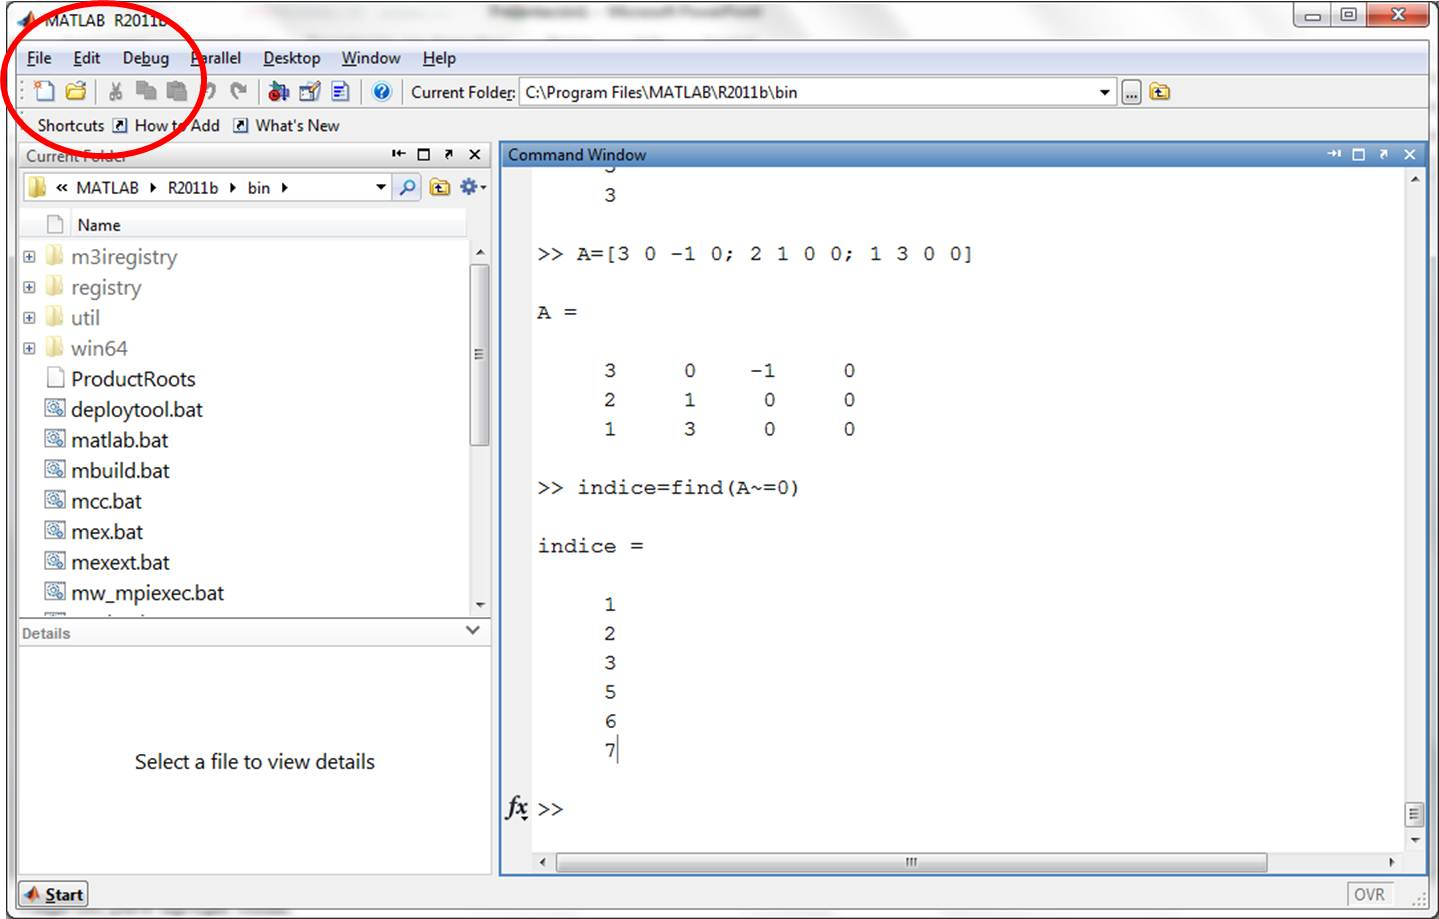
\includegraphics[width=14cm]{opened.pdf}
\caption{posición del menú File y del icono de nuevo documento en el IDE de Matlab}
\label{fig:opened}
\end{figure}

La otra opción es emplear el comando \texttt{edit}. Este comando puede emplearse de dos maneras. Si se escribe en la ventana de comandos,

\begin{verbatim}
>>edit
\end{verbatim}
Matlab abrirá el editor de textos y creará un documento nuevo sin nombre (\emph{untitled}.

Si añadimos a continuación del comando \texttt{edit} el nombre de un fichero,
\begin{verbatim}
>>edit ejemplo1.m
\end{verbatim}

Buscará un fichero con dicho nombre en los directorios de Matlab y en el directorio de trabajo. Si lo encuentra, abrirá el archivo encontrado. Si no lo encuentra, creará uno nuevo con dicho nombre. La figura \ref{fig:edv} muestra el editor de textos de Matlab, con el contenido del fichero \texttt{ejemplo1.m}. En dicha imagen es posible observar las barras de menú y de herramientas de las que dispone el editor de texto, para facilitar el trabajo de programación. 
\begin{figure}[h]
\centering
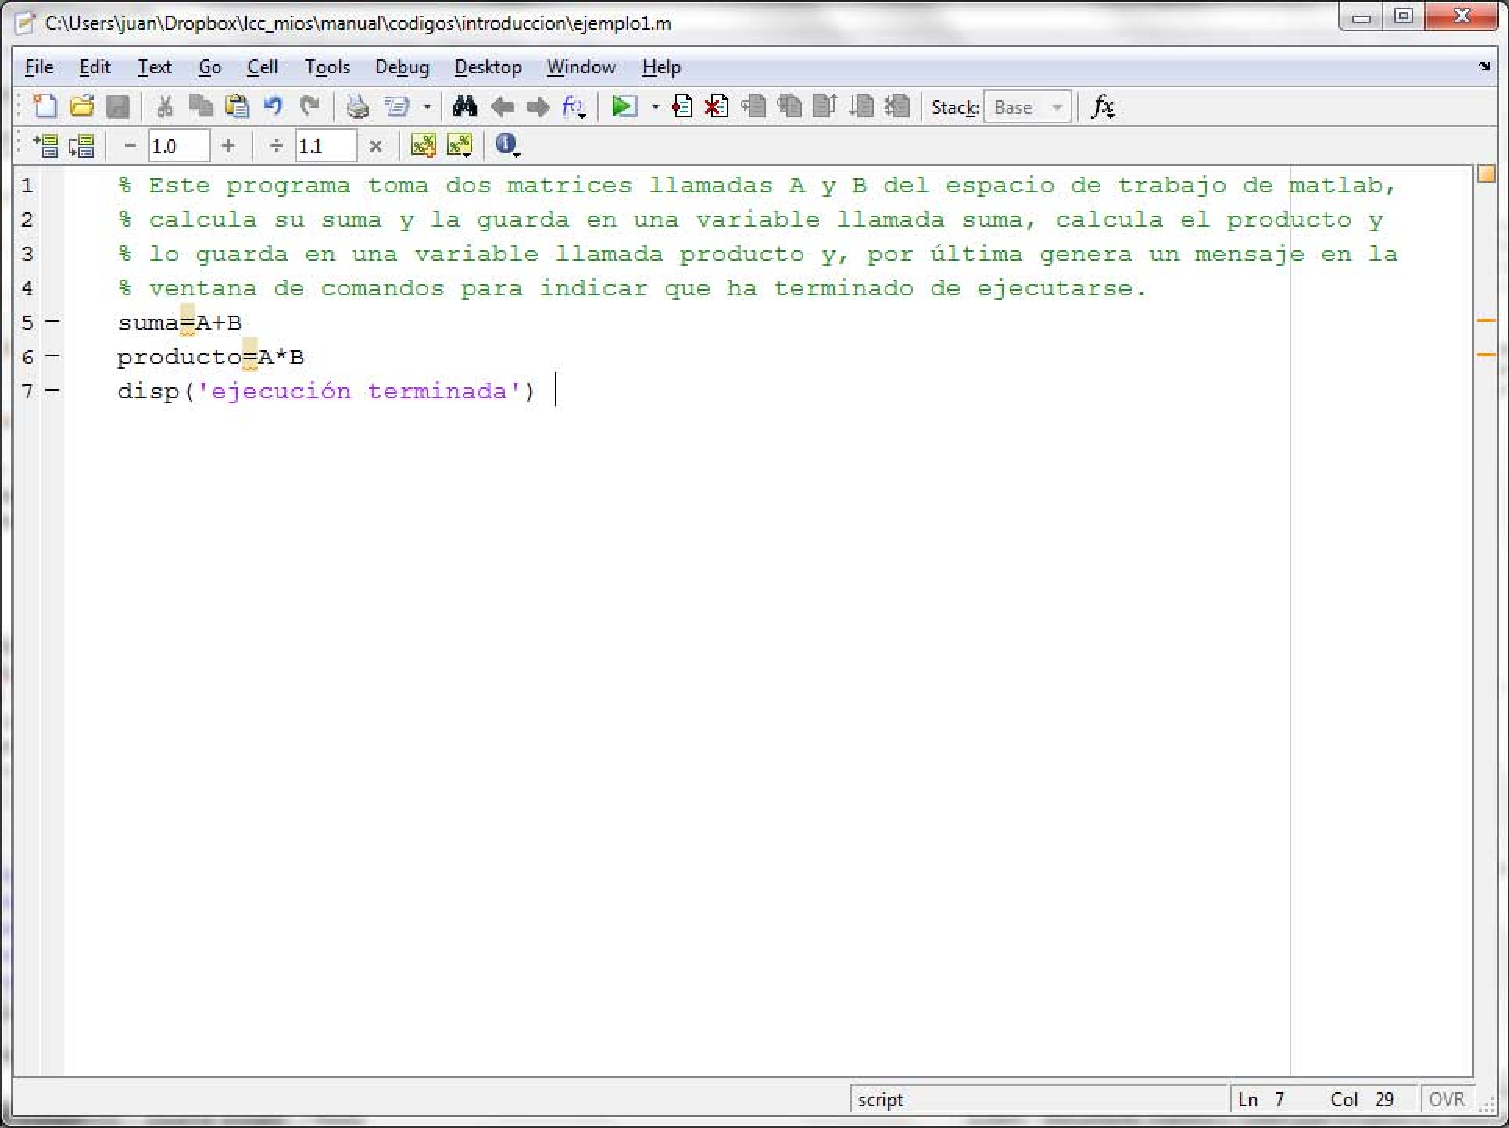
\includegraphics[width=14cm]{ejemplo1.pdf}
\caption{Vista del editor de textos de Matlab mostrando el contenido del fichero prueba1.m}
\label{fig:edv}
\end{figure}
Éstas, entre otras facilidades --resaltar texto de palabras clave, cotar número de líneas, sangrar estructuras de programación, etc.-- hacen que resulte especialmente atractivo emplear el editor de textos de Matlab en lugar de emplear otro editor de textos genérico.

\subsection{Scripts} \index{Script}
Un script en Matlab es un simple fichero de texto que contiene un conjunto de sentencias de Matlab válidas. La manera de ejecutarlo, consiste en escribir el nombre del fichero en la línea de comandos de Matlab. Matlab va leyendo el contenido del fichero línea a línea, y va ejecutando los comandos que contiene cada línea exactamente igual que si se hubieran escrito directamente en la línea de comandos de Matlab. Veamos un ejemplo sencillo, que corresponde con el código contenido en la figura \ref{fig:edv}:
\begin{verbatim}
% Este programa toma dos matrices llamadas A y B del espacio de trabajo de
%  Matlab, calcula su suma y la guarda en una variable llamada suma, calcula el 
% producto y lo guarda en una variable llamada producto y, por última genera un 
%mensaje en la ventana de comandos para indicar que ha terminado de ejecutarse.
suma=A+B
producto=A*B
disp('ejecución terminada') 
\end{verbatim}
Si escribimos el texto anterior en un archivo y lo guardamos con el nombre ejemplo1.m, podemos ejecutar su contenido en Matlab sin más que escribir en la línea de comandos:
\begin{verbatim}
>> ejemplo1
\end{verbatim}

Las cuatro primeras líneas de código que empiezan con el símbolo \% no se ejecutan. Cuando Matlab encuentra una línea que empieza con dicho símbolo interpreta que se trata de un comentario escrito por el programador, para explicar qué hace el programa o aclarar algún aspecto de su funcionamiento. Cuando el editor de Matlab detecta el símbolo \% en una línea de código, resalta en color verde todo el texto de la línea a partir de dicho símbolo. De este modo, es inmediato ver que se trata de un comentario y que Matlab no tratará de ejecutarlo.

Un aspecto importante de la programación en Matlab, y en cualquier otro lenguaje de programación, lo constituye el comentario del código de programa; facilita su uso por otros usuarios y permite al programador recordar qué fue lo que hizo cuando lo programó. La experiencia demuestra que, en poco tiempo, los programas no comentados se vuelven incompresibles incluso para quien los escribió.

La quinta línea del programa busca en el \emph{workspace} las variables \texttt{A} y \texttt{B}. Si las variables no existen, es decir, si no han sido creadas previamente, el programa da un error, exactamente igual que si hubiéramos escrito directamente en la ventana de comandos de Matlab la sentencia \texttt{suma=A+B} sin haber definido antes \texttt{A} y \texttt{B}. Si las variables existen calcula la suma y guarda el resultado en el \emph{workspace} en la variable \texttt{suma}. La siguiente línea de código realiza el cálculo del producto de las dos variables y guarda el resultado en la variable \texttt{producto}. La última línea del programa mostrará en la ventana de comandos la frase,

\begin{verbatim}
ejecución terminada
\end{verbatim}
Para ello emplea la función de Matlab \texttt{disp} que escribe en la ventana de comandos cadenas de caracteres.

Un aspecto muy importante de los \emph{scripts} es que hacen uso del \emph{workspace} de Matlab tanto para buscar las variables que emplean como para guardar las variables resultantes de sus cálculo. Su ejecución es idéntica a la que se realizaría si copiáramos línea a línea en la ventana de comandos y las fuéramos ejecutando una detrás de otra.

\subsection{Funciones} \index{Funciones! Definición de funciones en matlab}
Las funciones juegan un papel fundamental en cualquier lenguaje de programación. En el caso de Matlab, se escriben como ficheros de texto, de modo análogo a los \emph{scripts}. lo que determina que Matlab los interprete como funciones es su primera línea de código.  Nos referiremos a esta primera línea con el nombre de \emph{cabecera de la función}. La cabecera de una función debe empezar siempre por la palabra clave \texttt{function}. Debe contener además, como mínimo, el nombre de la función. Por ejemplo,
\begin{verbatim}
function raices
\end{verbatim}

Un detalle importante en Matlab es que el fichero de texto que contiene la función debe llamarse igual que ésta, para que Matlab pueda identificar la función correctamente. Es decir, en el caso del ejemplo anterior, el fichero que contenga la función debe llamarse raíces.m.

A parte del nombre de la función la cabecera puede incluir también nombres de las variables de entrada. Estos se escriben a continuación del nombre de la función, separadas por comas y encerradas entre paréntesis,

\begin{verbatim}
function raices(a,b,c)
\end{verbatim}

En este ejemplo \texttt{a}, \texttt{b} y \texttt{c} son variables de entrada de la función \texttt{raices}. La razón por la que hay que incluir estas variables de entrada es que, a diferencia de los \emph{scripts}, las funciones no pueden acceder directamente a los valores de las variables contenidos en el \emph{workspace} de Matlab. Cuando se ejecuta una función es preciso dar valores a las variables que necesite utilizar, y que no se definan expresamente en el código de la función. Aclararemos esto más tarde con un ejemplo.

Por último la cabecera de una función puede incluir también una o varias variables de salida. Estas se escriben delante del nombre de la función separadas por comas y encerradas entre corchetes. Entre la(s) variable(s) de salida y el nombre de la función se incluye el símbolo de asignación \texttt{=}, para indicar que los resultados obtenidos por la función se han asignado (guardado en) a dichas variables.

\begin{verbatim}
function [x1,x2]=raices(a,b,c)
\end{verbatim}
  
En este caso, las variables de salida serían \texttt{x1} y \texttt{x2}.

A continuación, vamos a completar el ejemplo para el que hemos construido la cabecera en los párrafos anteriores. Se trata de una función que obtiene las raíces de una ecuación de segundo grado, $ax^2+bx+c=0$ conocidos sus coeficientes $a, b, c$,
\begin{verbatim}
function [x1,x2]=raices(a,b,c)
%Esta función calcula las raices de una ecuación de segundo grado ax^2+b^x+c=0
%las variables de entrada son los coeficientes a, b, c de la ecuación. 
%las variables de salida x1 , x2 son las dos raices de la ecuación

%calculo de la primera raiz
x1=(-b+(b^2-4*a*c)^(1/2))/(2*a)

%calculo de la segunda raiz
x2=(-b-(b^2-4*a*c)^(1/2))/(2*a)
\end{verbatim}

Deberemos guardar estas líneas de código en un archivo con el nombre raices.m. Podemos ahora emplear la función \texttt(raices) para calcular las raíces de una ecuación de segundo grado. Supongamos que queremos obtener las raíces de la ecuación,
\begin{equation*}
x^2+x-6
\end{equation*}

si escribimos en la línea de comandos,
\begin{verbatim}
>>[raiz1, raiz2]=raices(1,1,-6)
\end{verbatim}
Matlab mostrará en la pantalla,

\begin{verbatim}
x1 =

     2
     
x2 =

    -3


raiz1 =

     2


raiz2 =

    -3

\end{verbatim}

Analicemos con un poco de detalle lo que hemos hecho. Al escribir: \texttt{[raiz1,raiz2] =} \texttt{raices (1,1,-6)}, hemos \emph{llamado} a la función \texttt{raices}, indicando que las variables de entrada deben tomar los valores \texttt{a=1},\texttt{b=1}, \texttt{c=-6}, es decir, los valores de los coeficientes de la ecuación de segundo grado cuya solución queremos obtener. Además hemos pedido a Matlab que guarde los resultados en el \emph{workspace} en las variable \texttt{raiz1} y \texttt{raiz2}. Cuando, tras llamar a la función, pulsamos el retorno de carro, Matlab empieza a ejecutar el código de la misma. Lo primero que hace es crear las variables \texttt{a}, \texttt{b} y \textbf{c} y asignarle los valores 1,1 y -6. Matlab crea estas variables pero no las guarda en el workspace sino en un espacio de memoria al que solo tiene acceso la función \texttt{raices}, desde la que se han creado. 
Esto constituye una característica muy importante de las funciones en Matlab. Cada vez que se llama a una función, se crea un espacio de memoria en la que se guardan las variable definidas en la función y a la que solo ésta tiene acceso. Además, una función no puede acceder ni modificar directamente ninguna variable que esté en el \emph{workspace}.

Una vez que la función ha asignado valores a las variable de entrada, comienza a realizar los cálculos pedidos, en primer lugar calcula la raíz correspondiente al discriminante positivo,
\begin{equation*}
+\sqrt{b^2-4ac}
\end{equation*}
y crea la variable \texttt{x1} para guardar el resultado. La variable \texttt{x1} solo existe en la memoria de la función \texttt{raices} y por tanto no existe ni es accesible desde el \emph{workspace}. Como no hemos terminado la línea de programa en la que se calcula \texttt{x1} con un punto y coma, Matlab muestra en la ventana de comandos el resultado del cálculo realizado. 

La raíz correspondiente al discriminante negativo se calcula de modo análogo. Una vez terminada la ejecución de la líneas del programa, Matlab vuelve a examinar la cabecera del programa y observa que debe dar como resultado, los valores contenidos en las variables \texttt{x1} y \texttt{x2}. Para ello, crea la variable \texttt{raiz1}  en el \emph{workspace} y copia en ella el contenido de la variable \texttt{x1}. Análogamente crea la variable \texttt{raiz2} y copia en ella el contenido de la variable \texttt{x2}. Con esto ha terminado la ejecución del programa. Matlab destruye las variables \texttt{x1} y \texttt{x2} que solo han existido durante la ejecución del programa, y nos muestra de nuevo el \emph{prompt} en la ventana de comandos para indicarnos que esta listo para ejecutar nuevas órdenes. Si analizamos el contenido del \emph{workspace}, empleando el comando \texttt{who} de Matlab,
\begin{verbatim}
>> who

Your variables are:

raiz1  raiz2  

\end{verbatim}
observaremos que allí están las variable \texttt{raiz1} y \texttt{raiz2}, que contienen las raíces de la ecuación de segundo grado que queríamos resolver.

En el ejemplo anterior hemos asignado directamente valores a las variables de entrada de la función \texttt{raices}. En Matlab, una función puede también asignar valores a sus variable de entrada copiándolos de los de otras variables existentes en el workspace, supongamos que creamos en el workspace de Matlab, tres variables con los valores de los coeficientes de la ecuación de segundo grado del ejemplo anterior,
\begin{verbatim}
>>coef1=1, coef2=1 coef3=-6
\end{verbatim}

Podríamos entonces llamar a nuestra función raíces, sustituyendo los valores de la variables de entrada por los nombres de éstas variables,

\begin{verbatim}
>> [raiz1, raiz2]= raices(coef1,coe2,coef3)
\end{verbatim} 
 Matlab, copiará ahora los valores contenidos en \texttt{coef1}, \texttt{coef2} y \texttt{coef3} en las variables de entrada de la función \texttt{a}, \texttt{b}, \texttt{c}. Ni que decir tiene, que el resultado final de la ejecución será el mismo.

\paragraph{Ámbito de una variable} \index{Variable! Ámbito de una variable}\index{Variable!Ámbito}La importancia del concepto de función está precisamente en el tratamiento que hace de las variables. Para entenderlo mejor, introduciremos el concepto de \emph{ámbito} de una variable.

Como hemos visto, la forma usual de crear una variable en Matlab es mediante el símbolo de asignación. Cuando asignamos un valor o el resultado de una operación a una variable en la ventana de comandos de Matlab,

\begin{verbatim}
>> a=18

a =

    18

\end{verbatim} 
 
Matlab reserva un espacio de memoria del computador para guardar la variable con el valor asignado. Esta variable forma parte del \emph{workspace} de Matlab, que constituye su ámbito propio. La variable creada es solo visible para aquellos comandos y sentencias que,
\begin{enumerate}
\item Se ejecutan desde la ventana de comandos de Matlab.
\item Se ejecutan desde un script.
\end{enumerate}

Cuando ejecutamos una función desde la ventana de comandos de Matlab, la función crea su propio espacio de memoria. Por así decir, es como un \emph{workspace} particular de la función. Cualquier variable que cree la función se guardará en el espacio de memoria de la función, que constituirá su ámbito propio. La variable creada dentro de la función solo es visible para aquellos comandos y sentencias que se ejecutan dentro de la función.

Una vez que termina la ejecución de una función, el espacio de memoria que se creó al ejecutarse se destruye y con él cualquier variable que el programa haya creado durante su ejecución.

La única manera de pasar información contenida en una variable del \emph{workspace} de Matlab a una función es copiándola a una variable de entrada de la función.

La única manera de pasar información contenida en una variable del espacio de memoria de una función, al workspace de Matlab, es copiándola a través de una variable de salida de la función.


\begin{figure}[h]
\centering
\begin{tikzpicture}
%\usetikzlibrary{shapes.multipart}
\path (5,0) node(a) [rectangle split,rectangle split parts =2,draw=blue,top color=white,bottom color=blue!15, very thick,align=left,rounded corners]{Ventana de comandos de Matlab
\nodepart{two}
\textgreater \textgreater a=3\\
\textgreater \textgreater b=2\\
\textgreater \textgreater y=ejem(a)\\
y =\\
    12\\
\textgreater \textgreater}		
(0,-7) node(b)[rectangle split,rectangle split parts =2,draw=blue, thick,rounded corners,align=left]{\emph{workspace de Matlab}\\
\nodepart{two}
a=3\\
b=2\\
...\\
tras ejecutar ejem\\
y=12
}
(10,-7) node(c)[rectangle split,rectangle split parts =2,draw=red,thick,rounded corners,align=left]{Espacio de memoria\\ de la funcion\\ \texttt{ejem.m}
\nodepart{two}
ent=3\\
b=4\\
sal=12\\
...\\
tras ejecutar ejem\\
se destruyen\\
todas las variables}
(5,-7) node(d)[rectangle,draw=red,top color=white, bottom color=red!15,align=left,very thick, rounded corners]{function sal=ejem(ent)\\ 
b=4;\\
sal=b*ent;}
(5,-5)node(e)[circle,draw=black,left color=blue!20,right color=red!20,thick,align=center]{Copiar\\ a en ent}
(5,-9)node(f)[circle,draw=black,left color=blue!20,right color=red!20,thick,align=center]{Copiar\\ sal en y};
\draw[blue,-latex](a.west)to [out=180, in=90]node[auto,swap]{Crea a y b} (b);
\draw[blue,-latex](a.south west)to [out=225, in=135]node[auto,align=center]{llamada a la\\ función\\ ejem($\cdot$)} (d.north west);
\draw[black,-latex](b.north east)to [out=45, in=180](e);
\draw[black,-latex](e.east)to [out=0, in=135](c.north west);
\draw[red,-latex](d.north)to [out=90, in=270](e);
\draw[black,-latex](c.south west)to [out=225, in=0](f);
\draw[black,-latex](f.west)to [out=180, in=315](b.south east);
\draw[red,-latex](d.south)to [out=270, in=90](f);
\draw[red,-latex](d.east)to node[auto,swap,align=center]{Crea b\\ y sal}(c);
\draw[red,-latex](d.north east)to [out=45, in=315]node[auto,align=center]{devolución\\ control\\ ventana de comandos} (a.south east);
\end{tikzpicture}
\caption{Ejemplo de uso de memoria y ámbito de variables durante la ejecución de una función}
\label{fig:amb}
\end{figure} 

La figura \ref{fig:amb} muestra esquemáticamente como se gestionan las variables en Matlab. En el cuadro superior se muestra la ejecución de varias sentencias en la ventana de trabajo de Matlab. Las dos primeras crean directamente dos variables \texttt{a} y \texttt{b} que se almacenan en el \emph{workspace de Matlab}, representado por el cuadro azul de la derecha. 
A continuación se llama a la función ejem (cuadro rojo central), asignándole como variable de entrada la variable \texttt{a} y como variable de salida la variable \texttt{y}. La ventana de comandos \emph{cede} el control a la función que empieza a ejecutarse:
\begin{enumerate}
\item La función crea su propio espacio de memoria (cuadro rojo de la izquierda)
\item Copia el valor contenido en la variable \texttt{a} en la variable \texttt{ent}. Esta variable se almacena en el espacio de memoria de la función.
\item Crea la variable \texttt{b} asignándole el valor 4 y la guarda en el espacio de memoria de la función. 

A partir de este momento y hasta el final de la ejecución de la función hay dos variables con el mismo nombre: \texttt{b=2} en el \emph{workspace} de Matlab; \texttt{b=4} en el espacio de memoria de la función. Las dos variables coexisten pero no se pueden confundir porque pertenecen a ámbitos distintos.
\item Crea la variable sal asignándole el producto de \texttt{b=4} por \texttt{ent=3}. Almacena la variable sal en el espacio de memoria de la función.
\item La función a llegado al final de su código. vuelve a leer la cabecera y crea la variable \texttt{y} en el workspace de Matlab, copiando el contenido de la variable \texttt{sal}.
\item termina la ejecución destruyendo el espacio de memoria de la función y \emph{devolviendo} el control a la ventana de comandos.
\end{enumerate}

\paragraph{Llamar a una función desde otra función.}
En Matlab, como en cualquier lenguaje de alto nivel, es posible llamar una función desde dentro de otra. Incluso es posible que una función se llame a sí misma, aunque este caso lo veremos más adelante cuando hablemos de control de flujo. 

Veamos un ejemplo sencillo de llamada de una función desde otra,

\begin{verbatim}
function salida=ejemplo2(entrada)
%esta funcion toma el valor de entrada lo eleva al cuadrado y pasa el
%resultado aun segunda función que calcula la raiz cuadrada...
%entrada y salida deberían ser iguales al final

x=entrada^2;

%%%%llamada a la segunda función%%%%
salida=raiz(x);
\end{verbatim}

La función \texttt{ejemplo2} llama a una segunda función \texttt{raiz} cuyo código,

\begin{verbatim}
function out=raiz(in)
out=in^(1/2);
\end{verbatim}

Debe guardarse en uno de los tres lugares siguientes:
\begin{enumerate}
\item En el mismo fichero, ejemplo2.m en que se encuentra escrito el código de la función \texttt{ejemplo2}, justo debajo de dicha función.
\item En un fichero propio, raiz.m guardado en el directorio en que Matlab está trabajando.
\item En un fichero propio, raiz.m guardado en cualquier directorio de los incluidos en el \emph{path} de Matlab.
\end{enumerate}

Además al ejecutar la función \texttt{ejemplo2}, se buscará el código de la función raíz, precisamente en el orden que acabamos de indicar. Si añadimos directemente el código de la función \texttt{raiz} al fichero ejemplo2.m, el código quedaría,

\begin{verbatim}
function salida=ejemplo2(entrada)
%esta funcion toma el valor de entrada lo eleva al cuadrado y pasa el
%resultado aun segunda función que calcula la raiz cuadrada...
%entrada y salida deberían ser iguales al final

x=entrada^2;

%%%%llamada a la segunda función%%%%
salida=raiz(x);

%%%%%%codigo de la segunda funcion%%%%%
function out=raiz(in)
disp('version incluida en el archivo ejemplo2.m')
out=in^(1/2);
\end{verbatim}

La ventaja de escribir el código de la segunda función en el mismo fichero de la primera es que el acceso es más rápido. Sin embargo, solo la función \texttt{ejemplo2} podrá llamarla. Es decir la función \texttt{raiz} no puede emplearse desde la ventana de comandos de Matlab  ni desde ninguna otra función.

En general, si escribimos en un archivo .m de Matlab varias funciones,

\begin{verbatim}
function a=uno(b)
%aqui viene el codigo de la funcion uno
...

function c=dos(d)
%aqui viene el codigo de la funcion dos
...

function e=tres(f)
%aqui viene el codigo de la funcion dos
...
.
.
.
\end{verbatim}

Todas las funciones incluidas en el fichero pueden llamarse entre unas a otras, pero solo la primera de ellas puede ser ejecutada desde la ventana de comandos de Matlab. Además el nombre del fichero debe coincidir con el nombre de la primera función  contenida en él. En el ejemplo que acabamos de esbozar, el fichero debería llamarse uno.m.

Evidentemente si cada función está guardada en un fichero .m distinto, todas las funciones pueden en principio ser ejecutadas desde otra función o desde la ventana de comandos de Matlab.

Cada vez que se ejecuta una función, ésta crea su propio espacio de memoria. Las variables incluidas en la cabecera de la función como variables de entrada y salida se copian, tal y como hemos visto para el caso de una función simple, entre el espacio de memoria propio de la función y el espacio de memoria de la función que la ha llamado.

  
\subsection{Funciones incluidas en Matlab.}\index{Funciónes! Funciones incluidas en matlab} 
Matlab incluye cientos de funciones. Estas funciones, están escritas con la misma filosofía que acabamos de describir aquí, es decir, admiten una o varias variables de entrada y devuelven sus resultados en una o varias funciones de salida. En algunos casos, se trata de ficheros de texto  guardados con la extensión \texttt{.m} iguales a los que nosotros podemos crear \footnote{En muchos casos las funciones incluidas en Matlab no están escritas en ficheros de texto accesibles para el usuario. Por razones de eficiencia, se trata de versiones de las funciones escritas por lo general en lenguaje C y compiladas.}. La manera de emplearlas desde la ventana de comandos de Matlab es idéntica a la descrita para las funciones creadas por el usuario. 

En la tabla \ref{tabfun}, se incluyen algunos ejemplos de las funciones matemáticas más corrientes. Son solo una pequeña muestra de las funciones disponibles. Para obtener una visión más completa de las funciones disponibles se aconseja emplear la ayuda de Matlab.

\begin{table}
\caption{Algunas funciones matemáticas en Matlab de uso frecuente}
\label{tabfun}
\begin{tabular}{c|c|c|c}
tipo&nombre&variables&función matemática\\
\hline
\hline
Trigonométrica&cos&y=cos(x)&coseno de un ángulo en radianes\\
\hline
Trigonométrica&sin&y=sin(x)&seno de un ángulo en radianes\\
\hline
Trigonométricas&tan&y=tan(x)&tangente de un ángulo en radianes\\
\hline
Trigonométricas&csc&y=csc(x)&cosecante de un ángulo en radianes\\
\hline
Trigonométricas&sec&y=sec(x)&secante de un ángulo en radianes\\
\hline
Trigonométricas&cot&y=cot(x)&cotangente de un ángulo en radianes\\

\hline
Trigonométricas&...&y=a...(x)&inversa de una función trigonométrica en radianes\\
&asin&y=asin(x)&ejemplo, arcoseno en radianes\\
\hline
\hline
Exponencial&exp&y=exp(x)&$e^x$\\
\hline
Exponencial&log&y=log(x)&logaritmo natural\\
\hline
Exponencial&log10&log10(x)&logaritmo en base 10\\
\hline
Exponecial&sqrt&y=sqrt(x)&$\sqrt(x)$\\
\hline
\hline
Redondeo&ceil&y=ceil(x)& redondeo hacia $+\infty$\\
\hline
Redondeo&floor&y=floor(x)&redondeo hacia $-\infty$\\
\hline
Redondeo&round&y=round(x)&redondeo al entero más próximo\\
\hline
Redondeo&fix&y=fix(x)&redondeo hacia $0$\\
\hline
Redondeo&rem&r=rem(x,y)&resto de la división entera de y entre x\\
\hline
\hline
Módulos&norm&y=norm(x)& módulo de un vector x\\
\hline
Módulos&abs&y=abs(x)&valor absoluto de x,(módulo de x si x es complejo)\\
\hline
Módulos&sign&y=sign(x)&función signo; 1 si x $>$ 0, -1 si x $<$ 0, 0 si x=0\\
\end{tabular}
\end{table}

\subsection{Depuración.}\index{Depurador}
Siempre que escribimos un programa, tanto si se trata de un \emph{script} como si es una función, es preciso comprobar su funcionamiento y, en  muchos casos corregir los errores cometido. El proceso de corrección de código desde su versión original hasta la versión definitiva se conoce con el nombre de depuración de código. Podemos distinguir dos tipos fundamentales de errores:

\begin{enumerate} 
\item Errores de sintaxis. \index{Error! De sintáxis}Normalmente son errores de escritura. Hemos escrito mal el nombre de una función o un comando o bien no hemos escrito correctamente el código siguiendo las reglas del lenguaje. Matlab advierte directamente de estos errores, cuando se trata de ejecutar el código, escribiendo en la ventana de comandos un mensaje de error. Como ejemplo veamos los errores del siguiente \texttt{script},

\begin{verbatim}
%script con errores,
y=[1 2 3; 4 5 6; 2 3] %a esta matriz le falta un elemento en la última fila

x=[1 2 3; 4 5 6]
z=y*x %las matrices no pueden multiplicarse entre si por que no coinciden
      %numero de columnas de la primera con numero de filas de la segunda
\end{verbatim}

Si observamos el editor de textos, \ref{fig:ederror} puede observarse algunas de los caracteres del texto subrayados en rojo. Esto puede indicar la existencia de errores en esa línea de código, como en el caso del carácter que se ha rodeado en la figura de un círculo rojo. 

En otros casos, --circulos azules de la figura-- se trata de advertencias, el programa funciona pero puede hacerlo de forma más eficiente; en el caso de la figura simplemente nos sugiere que añadamos un punto y coma al final de las sentencias, para que Matlab no escriba el resultado de cada cálculo en la ventana de comandos. No se trata por tanto de errores sino de advertir al programador que con puntos y comas su programa se ejecutará más rápido.

\begin{figure}[h]
\centering
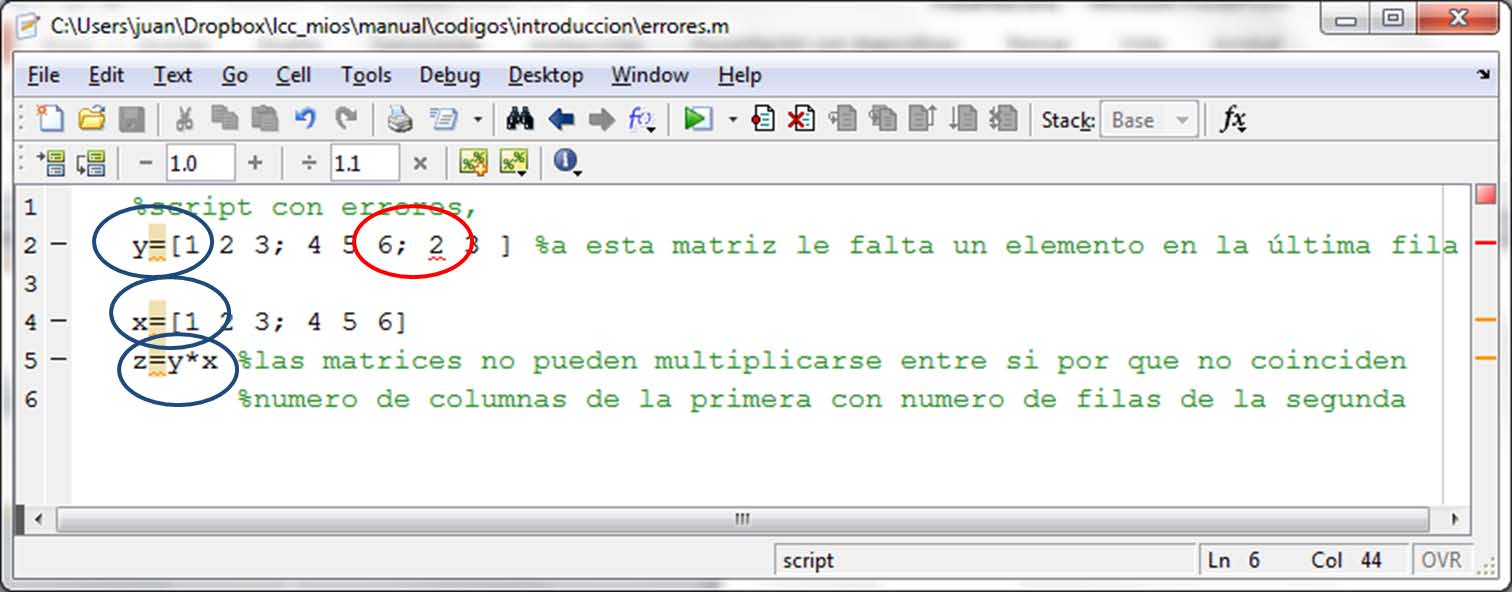
\includegraphics[width=14cm]{errores.pdf}
\caption{Vista de el editor de texto de Matlab. Circulo rojo error en el código. Circulos azules advertencias de posible mejoras}
\label{fig:ederror}
\end{figure}

Si ejecutamos el script, que hemos guardado con el nombre de \texttt{errores.m},

\begin{verbatim}
>> errores
Warning: File: errores.m Line: 2 Column: 4

The expression on this line will generate an error when executed.  
The error will be:  Error using vertcat
CAT arguments dimensions are not consistent.
 
Error using errores (line 2)
Error using vertcat
CAT arguments dimensions are not consistent.
\end{verbatim}

Matlab ha detectado el error en la construcción de la matriz \texttt{y}, nos indica el tipo de error cometido y la línea y columna de código donde se ha producido.

Si corregimos el código, añadiendo a la matriz \texttt{y} el elemento que le falta,

\begin{verbatim}
%script con errores,
y=[1 2 3; 4 5 6; 2 3 8] %Ultima fila completada
x=[1 2 3; 4 5 6]
z=y*x %las matrices no pueden multiplicarse entre si por que no coinciden
      %numero de columnas de la primera con numero de filas de la segunda
\end{verbatim}
y volvemos a ejecutar el script.
\begin{verbatim}
>> errores

y =

     1     2     3
     4     5     6
     2     3     8


x =

     1     2     3
     4     5     6

Error using  * 
Inner matrix dimensions must agree.

Error in errores (line 5)
z=y*x %las matrices no pueden multiplicarse entre si por que no coinciden
\end{verbatim}
Matlab nos detecta el siguiente error cometido así como la línea en la que se comete. 

Si intercambiamos las posiciones entre las variables \texttt{x} e \texttt{y} en el producto, suponiendo que ésta es la causa del error cometido,

\begin{verbatim}
y=[1 2 3; 4 5 6; 2 3 8] 

x=[1 2 3; 4 5 6]
z=x*y 
\end{verbatim}

El código se ejecuta con normalidad,
\begin{verbatim}
>> errores

y =

     1     2     3
     4     5     6
     2     3     8


x =

     1     2     3
     4     5     6


z =

    15    21    39
    36    51    90
\end{verbatim}

\item Errores de codificación.\index{Errores! De codificación} Este segundo tipo de errores son mucho más difíciles de detectar. El código se ejecuta sin problemas, pero los resultados no son los esperados. Ante esta situación, no queda más remedio que ir revisando el código, paso a paso para detectar donde está el error.

El siguiente código del script \texttt{trect.m} muestra un error de este tipo, 

\begin{verbatim}
%este script toma los valores de los catetos de un triángulo rectangulo del 
%workspace de Matlab (variables a y b). calcula su hipotenusa, y a partir
%de estos datos, el seno el coseno y la tangente del angulo formado por la
%hipotenusa y el cateto mayor que será siempre a

%calculo hipotenusa,

h=sqrt(a^2+b^2)

%calculo del seno

s=a/h

%calculo del coseno
a=b/h %error estamos sobreescriesdo el valor del coseno en la variable que 
      %guardaba el valor del cateto

%calculo de la tangente
t=b/a

\end{verbatim}

El programa funciona perfectamente, por ejemplo si hacemos \texttt{a=4} y \texttt{b}=3,

\begin{verbatim}
>> trect

h =

     5


s =

    0.8000


a =

    0.6000


t =

     5
\end{verbatim}
Como hemos sobre escrito en \texttt{a} el valor del coseno, cuando tratamos de utilizar dicha variable, como si fuera el cateto mayor, para obtener la tangente el resultado que obtenemos es erróneo.

El editor de texto de Matlab nos permite ejecutar un programa paso a paso, ver los valores que van tomando las variable en Matlab, etc, mediante el depurador que lleva incorporado. Para ello, se definen en el editor de Matlab \emph{breakpoints},esto es líneas en las cuales Matlab detendrá la ejecución de un programa, entrará en modo de depuración y esperará instrucciones del usuario. La figura \ref{fig:depu1} muestra el código del ejemplo que acabamos de ver, en el que se ha definido un \texttt{breakpoint}, pinchando con el ratón sobre el guión que precede a la línea del programa en la que se desea parar la ejecución. Matlab indica que el \emph{breakpoint} está activo, cambiando el guión por un círculo rojo.

\begin{figure}[h]
\centering
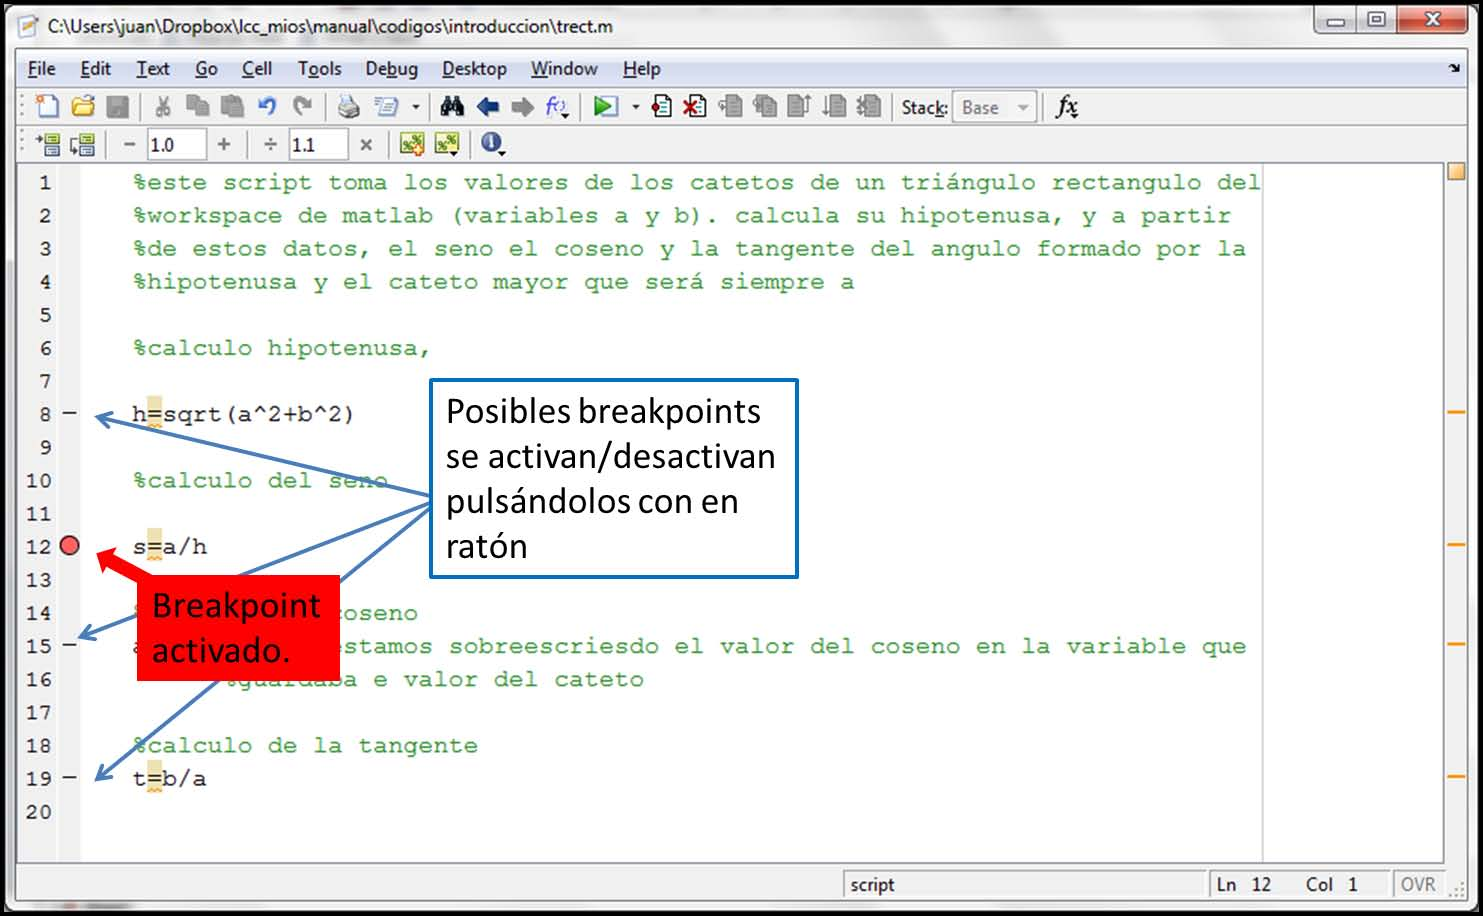
\includegraphics[width=14cm]{depu1.pdf}
\caption{Breakpoint activo}
\label{fig:depu1}
\end{figure}

Si una vez señalado el \emph{breakpoint}, ejecutamos el \emph{script},
\begin{verbatim}
>> trect

h =

    3.1477

12  s=a/h
K>> 
\end{verbatim}

Matlab nos indica que ha detenido la ejecución del programa en la línea marcada por el \emph{breakpoint} (línea 12 en el ejemplo). además vuelve a mostrar el \emph{prompt} en la ventana de comandos, pero esta vez precedido por la letra \texttt{k}, para indicarnos que ha entrado en modo de depuración.

A partir de aquí Matlab pone a nuestra disposición las herramientas de depuración, la figura \ref{fig:depu2} muestra la línea en que se ha parado la ejecución del programa, señalada con una flecha verde, y algunas de estas herraminentas. Básicamente nos da la posibilidad de ejecutar el código paso a paso, de entrar e ir paso a paso en las funciones que llama nuestro programa, o de de continuar la ejecución hasta que el final del programa o hasta el siguiente \emph{brakpoint} activo. Para dominar los detalles del depurador se aconseja leer la ayuda de Matlab.


\begin{figure}[h]
\centering
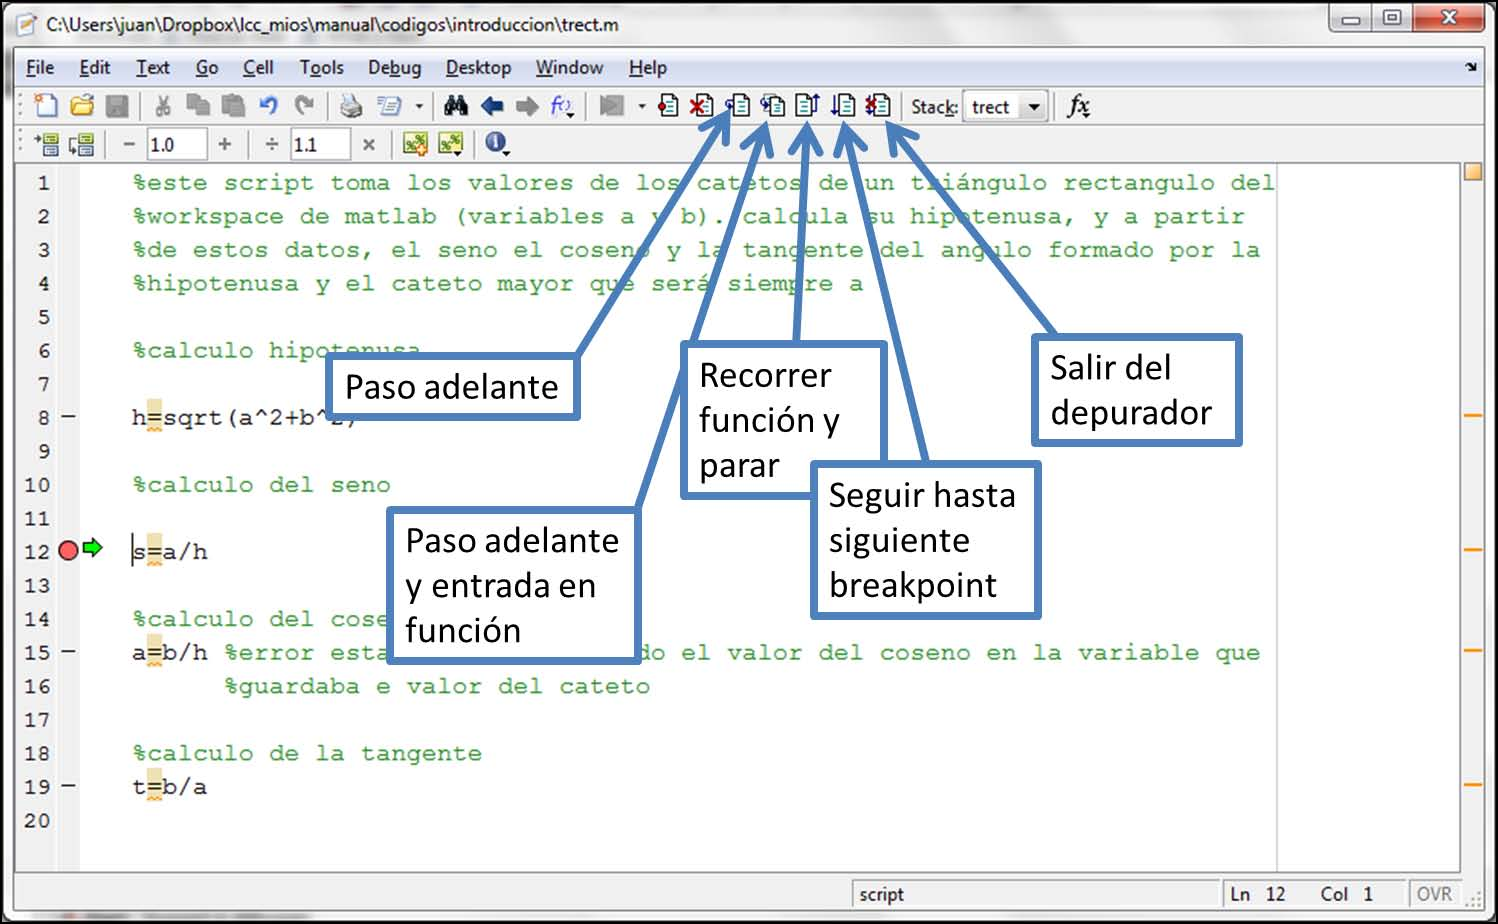
\includegraphics[width=14cm]{depu2.pdf}
\caption{Parada de programa en breakpoint y herramientas de depuración}
\label{fig:depu2}
\end{figure}

Si pulsamos el botón de "paso adelante" Matlab ejecutará la línea de programa señalada con la flecha verde y se parará en la línea siguiente. En cada paso, podemos ver el valor que toman las variables, pidiendo su valor directamente en la ventana de comandos,

\begin{verbatim}
K>> a

a =

    0.9531
\end{verbatim}

o bien señalando (sin pulsar botones) con el ratón en el editor de texto la variable de la que se trate.
En nuestro ejemplo del triángulo rectángulo es muy sencillo avanzar paso a paso en el programa con el depurador, y caer en la cuenta que, cuando se va a calcular la tangente, la variable \texttt{a} ya no contiene el valor del cateto.

\item Advertencias. \index{Advertencias} \index{Warnning}Por último señalar la existencia de los \emph{warnings} no se trata propiamente de errores, sino de simples advertencias de que algo puede funcionar de forma más eficiente, o puede no dar el resultado que esperábamos. En general, cuando se recibe un \emph{warning} al ejecutar un programa, o cuando el editor de Matlab subraya en rojo algún carácter en el editor de textos, se debe corregir el programa para que desaparezcan, aunque propiamente no se trate de errores.
\end{enumerate} 


 




\section{Control de Flujo}\index{Flujo} \index{Control de flujo}
En la sección anterior, se introdujo el modo de escribir programas en Matlab mediante el uso de 	\emph{scripts} y funciones. En todos los casos vistos, la ejecución del programa empezaba por la primera línea del programa, y continuaba, por orden, línea tras línea hasta alcanzar el final del programa. Se trata de programas en los que el \emph{flujo} es lineal, porque los resultados de cada línea de programa se van obteniendo regularmente uno detrás de otro. 

Hay ocasiones en las que, por diferentes razones que expondremos a continuación, puede interesarnos alterar el orden en que se ejecutan las sentencias de un programa, bien repitiendo una parte de los cálculos un determinado número de veces o bien ejecutando unas partes de código u otras en función de que se satisfagan unas determinadas condiciones.

El control del orden en que se ejecutan las sentencias de un programa es lo que se conoce con el nombre de \emph{control de flujo}. Veremos dos tipos principales de control de flujo: El flujo condicional y los bucles.
\subsection{Flujo condicional.}\index{Flujo!Condicional}
Empezaremos con un ejemplo sencillo de cómo y para qué condicionar el flujo de un programa. Supongamos que queremos construir un programa que reciba como variable de entrada un número cualquiera y nos muestra un mensaje por pantalla si el número es par.

Para ello, podríamos hacer uso de la función \texttt{rem} (ver tabla \ref{tabfun}). Si el resto de la división entre dos del número suministrado a la función es cero, se trata de un número par; si no, es un número impar. Podríamos hacer uso de operadores relacionales, en particular de \texttt{==} para comprobar si el resto de la división entre dos es cero. Por último necesitaríamos algún mecanismo que permitiera al programa escribir un mensaje solo cuando el número introducido sea par.

\paragraph{if - elseif - else - end.} El mecanismo que necesitamos nos lo suministra la estructura \texttt{if} de Matlab. Veamos en primer lugar el código del ejemplo del que venimos hablando,

\begin{verbatim}
function espar(x)
%Este programa recibe un numero entero como variable de entrada. y muestra
%por pantalla un mensaje indicando si el numero recibido es par o impar.

%Calculamos el resto de la division por dos
resto=rem(x,2);

%Empleamos una estructura if - else -end para decidir que mensaje mostrar

if resto==0
    %si el resto es cero el número es par
    disp('el número es par')
end
\end{verbatim}

El programa toma un número como variable de entrada y calcula el resto de su división entre dos. A continuación entra en una parte de código especial, que se inicia con la palabra clave \texttt{if} y termina con la palabra clave \texttt{end}. 

La palabra clave \texttt{if} va siempre seguida de una expresión que da un resultado lógico: verdadero ($1$) o falso ($0$). Esta expresión puede ser cualquier combinación válida de expresiones relacionales o lógicas. Esta expresión lógica, que sigue al if constituye una condición. El programa seguirá ejecutando las siguientes líneas solo si la condición se cumple; si no, se las saltará hasta llegar a la expresión \texttt{end}.

En nuestro ejemplo, se emplea una expresión relacional sencilla \texttt{resto==0}. Si se cumple, el programa ejecutará la siguiente línea de programa, escribiendo en la ventana de comandos la frase ``el número es par"  si no se cumple el programa se la salta, llega hasta el \texttt{end}, y no escribe nada por pantalla. 

Acabamos de ver la estructura condicional \texttt{if} más sencilla posible. Podríamos complicarla un poco pidiendo que también nos saque un mensaje por pantalla cuando el número sea impar. Esto supone incluir en nuestro programa una disyuntiva; si es par el programa debe hacer una cosa y si no, debe hacer otra. Para incluir este tipo de disyuntivas en una estructura \texttt{if}, se emplea la palabra clave \texttt{else}. Veamos nuestro ejemplo modificado,
\begin{verbatim}
function espar(x)
%Este programa recibe un numero entero como variable de entrada. y muestra
%por pantalla un mensaje indicando si el numero recibido es par o impar.

%Calculamos el resto de la division por dos
resto=rem(x,2);

%Empleamos una estructura if - else -end para decidir que mensaje mostrar

if resto==0
    %si el resto es cero el número es par
    disp('el número es par')
else
    %si el resto no es cero el número es impar
    disp('el número es impar')
end 
\end{verbatim}

La palabra clave \texttt{else} marca ahora la disyuntiva, si el número es par, el programa ejecuta las líneas de código entre el \texttt{if} y el \texttt{else}, si el número no es par ejecutará las líneas entre el \texttt{else} y el \texttt{end}.

La estructura \texttt{if} admite todavía ampliar el número de posibilidades de elección mediante la palabra clave \texttt{elseif}. Al igual que  con \texttt{if}, \texttt{elseif} va seguido de una expresión lógica que establece una condición, si se cumple se ejecutará el código de las líneas siguientes, si no se cumple, el programa saltará a la siguiente línea que contenga una palabra clave: otro \texttt{elseif}, un \texttt{else} o directamente el \texttt{end} que marca el final de la parte de código condicional. Para ver cómo funciona, vamos a modificar nuestro ejemplo anterior, para que, si el número introducido no es divisible por dos, compruebe si es divisible por tres,

\begin{verbatim}
function divis(x)
%Este programa recibe un numero entero como variable de entrada. y muestra
%por pantalla un mensaje indicando si el numero recibido es par. Si no es
%par, comprueba si es divisible por 3 y si lo es muestra un mensaje por  
%pantalla indicandolo. Si no es par ni divisible por tres muestra un
%mensaje diciendo que no es par ni disible por tres. 



%Empleamos una estructura if-elseif-else-end para decidir que mensaje mostrar

if rem(x,2)==0
    %si el resto es cero el número es par
    disp('el número es par')
elseif rem(x,3)==0
    %El número es divisible por tres
    disp('el número es divisible por 3')
else
    %el numero no es par ni divisible por tres
    disp('el número no es par ni divisible por 3')
end
\end{verbatim}

Si llamamos ahora a la función dando como valor de entrada un número par, Ejecutará el código situado debajo del \texttt{if} y antes del \texttt{elseif} y se saltará todo lo demás hasta llegar al \texttt{end}. Si el número introducido no es par, pero es divisible por tres, se saltará el código situado por debajo del \texttt{if}, ejecutará el código contenido debajo del \texttt{elseif} hasta el \texttt{else} y saltará el resto del código hasta llegar al \texttt{end}. Por último si el número no es par ni divisible por tres, solo ejecutará el código situado por debajo del \texttt{else}.

Un aspecto que debemos resaltar, es que el programa ejecutará el código correspondiente a la primera condición que se cumpla, y se saltará el resto hasta llegar al \texttt{end}. Así por ejemplo, si en nuestro ejemplo introducimos el número $6$, el programa nos mostrará el mensaje ``el número es par", puesto que ésta es la primera condición que se cumple, pero nunca nos mostrará el mensaje ``el número es divisible por 3". Porque una vez comprobada y cumplida la primera condición (ser par) el programa salta directamente al \texttt{end} final de la estructura, sin comprobar nada más. La figura \ref{fig:if} muestra el esquema completo de una estructura \texttt{if}. Los términos entre paréntesis pueden estar o no presentes en una implementación concreta.

\begin{figure}[h]
\centering
\begin{tikzpicture}
%\usetikzlibrary{shapes.multipart}
\path (5,0) node(a) [rectangle split,rectangle split parts =2,draw=blue,top color=white,bottom color=blue!15, very thick,align=left,rounded corners]{Estructura if-elseif-else-end
\nodepart{two}

if condición\\
\ \ \ ... código\\
\ \ \ ...\\
(elseif condición)\\
\ \ \ ... código\\
\ \ \ ...\\
(elseif condición)\\
\ \ \ ... código\\
\ \ \ ...\\
.\\
(puede haber tantos bloques elseif como se necesiten)\\
.\\
(else)\\
\ \ \ ... código\\
\ \ \ ...\\
end};		
\end{tikzpicture}
\caption{Esquema general de la estructura de flujo condicional \texttt{if} los términos escritos entre paréntesis son opcionales.}
\label{fig:if}
\end{figure} 

\paragraph{Estructuras if anidadas.}\index{Anidación! If anidado} 
En el ejemplo anterior, hemos visto cómo, si el número introducido en la función era par y además divisible por tres, el programa nunca nos informaría de esta segunda propiedad, debido al carácter excluyente de la estructura \emph{if}. Una manera de resolver este problema, es mediante el uso de estructuras \texttt{if} anidadas. La idea es muy sencilla, se construye una estructura \texttt{if} para comprobar una determinada condición, si esta se cumple, dentro de su código se construye otra estructura if para comprobar una segunda condición, y así sucesivamente, todas las veces que sea necesario. Si modificamos nuestro ejemplo anterior, incluyendo un \texttt{if} anidado,

\begin{verbatim}
function divis23(x)
%Este programa recibe un numero entero como variable de entrada. y muestra
%por pantalla un mensaje indicando si el numero recibido es par. 
%si el numero es par y divisible entre tres,
%si es divisible entre tres  
%Si no es par ni divisible por tres 



%Empleamos una estructura if - else -end 
%y un if anidado para decidir que mensaje mostrar

if rem(x,2)==0
    %si el resto es cero el número es par
    %comprobamos con un if anidado si además es divisible entre tres
    if rem(x,3)==0
        disp('el número es par y divisible entre tres')
    else
        disp('el número es par')
    end
elseif rem(x,3)==0
    %El número es divisble entre tres
    disp('el número es divisible entre 3')
else
    %el numero no es par ni divisible entre tres
    disp('el número no es par ni divisible entre tres')
end
\end{verbatim}

\paragraph{Switch-case-otherwise.} \index{Flujo! Switch-case}Se trata de otra estructura que permite también ejecutar una parte u otra de código de acuerdo con unas codiciones preestablecida. Estas condiciones se presentan en forma de \emph{casos}, el programa comprueba al llegar a la estructura \texttt{switch} de qué caso se trata y ejecuta el código correspondiente. La figura \ref{fig:switch} muestra la forma general que toma una estructura \texttt{switch}.

La estructura \texttt{switch}, compara el valor contenido en la variable de entrada a la estructura con las expresiones contenidas en los casos, ejecutando el primer caso para el que coincidan. Si no encuentra ninguno, ejecuta entonces el código contenido debajo de la sentencia \texttt{otherwise}.

Veamos un ejemplo muy sencillo,

\begin{verbatim}
function signo(x)
%este programa emplea una estructura switch para informarnos del signo de
%un número.

%NOTA EL PROGRAMA NO COMPRUEBA QUE LA VARIABLE DE ENTRADA X SEA UN NUMERO,
%SI ES UN VECTOR O UNA MATRIZEL RESULTADO NO TIENE SENTIDO
  
s=sign(x); %obtnemos el signo del número mediante la función sign

%construimos la estructura switch,

switch s
    case 1
        disp('el número es positivo')
    case -1
        disp('el número es negativo')
    otherwise
        disp('el número es cero')
end

\end{verbatim}

\begin{figure}[h]
\centering
\begin{tikzpicture}
%\usetikzlibrary{shapes.multipart}
\path (5,0) node(a) [rectangle split,rectangle split parts =2,draw=green,top color=white,bottom color=green!20, very thick,align=left,rounded corners]{Estructura switch-case-otherwise
\nodepart{two}
switch variable\\
\ \ \ case expresión\\
\ \ \ \ \ ... código\\
\ \ \ case expresión\\
\ \ \ \ \ ... código\\
\ \ \ .\\
Puede haber tantos bloques \emph{case} como se necesiten\\
\ \ \ .\\
\ \ \ otherwise\\
\ \ \ \ \ ... código\\
end};		
\end{tikzpicture}
\caption{Esquema general de la estructura switch-case-otherwise}
\label{fig:switch}
\end{figure}

La función del ejemplo emplea a su vez la función de Matlab \texttt{sign} para obtener el signo ($1$, $-1$, $0$) del número introducido. Guarda el resultado de esta operación en la variable \texttt{s}, que será precisamente la variable de entrada a la estructura \texttt{switch}. Los casos se limitan a chequear los posibles valores de la variable y enviar a la ventana de comandos el mensaje correspondiente.
 
\subsection{Bucles}\index{Flujo!Bucles}\index{Bucles}
En ocasiones, es preciso repetir una operación un número determinado de veces o hasta que se cumple una cierta condición. Los lenguajes de alto nivel poseen estructuras específicas, para repetir la ejecución de un trozo de programa las veces que sea necesario. Cada repetición recibe el nombre de iteración. Estas estructuras reciben el nombre genérico de bucles. Vamos a ver dos tipos: los bucles \texttt{for} y los bucles \texttt{while}.

\paragraph{Bucles for.} \index{Flujo! Bucle for}\index{Bucles! Bucle for}Un bucle \texttt{for} repite las sentencias contenidas en el bucle un determinado número de veces, es decir realiza un número fijo de iteraciones. La estructura general de un bucle \texttt{for} se muestra en la figura, \ref{fig:for}

\begin{figure}[h]
\centering
\begin{tikzpicture}
%\usetikzlibrary{shapes.multipart}
\path (5,0) node(a) [rectangle split,rectangle split parts =2,draw=orange,top color=white,bottom color=orange!30, very thick,align=left,rounded corners]{Estructura de un bucle for
\nodepart{two}

for indice=[vector de valores]\\
\ \ \ ... código\\
(condición: Break)\\
\ \ \ ...\\
(condicición: Continue)\\
\ \ \ ... código\\

end};		
\end{tikzpicture}
\caption{Esquema general de la estructura de un bucle \texttt{for} los términos escritos entre paréntesis son opcionales.}
\label{fig:for}
\end{figure} 
 
El bucle empieza con la palabra clave for, seguida de una variable a la que hemos dado el nombre genérico de índice. Esta variable irá tomando sucesivamente los valores de los elementos contenidos en el [vector de valores]. El código contenido en el bucle, desde la línea siguiente al \texttt{for} hasta el \texttt{end} se ejecutará tantas veces como valores tenga el vector de valores. Antes de hablar de las sentencias \texttt{break} y \texttt{continue}, veamos alguno ejemplos.
\begin{verbatim}
function y=demofor(x)
%este programa emplea un bucle for sencillo para ir mostrando uno a uno
%los elementos del vector de entrada x por pantalla. además los suma y 
%guarda el resultado total en el vector y,

y=0; %iniciamos la suma a cero

for i=x
    disp(i)
    y=y+i;
end
\end{verbatim}

Si ejecutamos el programa, usando como entrada el vector \texttt{d=[1 9 4 18]},

\begin{verbatim}
>> d=[1 9 4 18]

d =

     1     9     4    18

>> suma=demofor(d)
     1

     9

     4

    18


suma =

    32
\end{verbatim}

Una vez que el programa llega al bucle \texttt{for}, iguala la variable \texttt{i} al primer valor contenido en el vector de entrada, lo muestra por pantalla y añade su valor a la variable de salida. cuando llega al \texttt{end} del bucle for comprueba que todavía quedan valores del vector de entrada por recorrer, así que vuelve al principio del \texttt{for}, igual la variable \texttt{i} al segundo valor del vector de entrada, suma dicho valor a la variable de salida, llega al \texttt{end} y así sucesivamente hasta que haya recorrido todos los valores del vector de entrada.

El uso más habitual de los bucles, es para recorrer elementos de un vector o de una matriz. por esta razón, lo más frecuente es que no se de explícitamente el vector cuyos elementos debe recorrer el índice del \texttt{for}, sino que se construya empleado el operador \texttt{:},
\begin{verbatim}
for indice=principio:incremento:final
\end{verbatim}

Veamos un ejemplo sencillo para obtener el vector suma de dos vectores,
\begin{verbatim}
function s=sumafor(x,y)
%este programa emplea un bucle for sencillo para sumar dos vectores
%primero comprueba si son del mismo tamaño. Si no lo son da un mensaje de
%aviso

l1=length(x);
l2=length(y);
if l1==l2
    %construimos un vector de ceros del mismo tamaño que x e y paraa
    %guardar el resultado de la suma,
    s=zeros(size(x));
    %si son iguales los suma elemento a elemento usando un bucle for
    for i=1:l1
        s(i)=x(i)+y(i);
    end
else
    disp('los vectores son de distinto tamaño')
end
\end{verbatim}

En la figura \ref{fig:for}, aparecen dos sentencias opcionales, \texttt{break} y \texttt{continue}.

La sentencia \texttt{break}, permite terminar el bucle \texttt{for} antes de que haya terminado de realizar todas las ejecuciones previstas. La sentencia break va siempre incluida dentro de una condición que, si se cumple interrumpe la ejecución del bucle. Por ejemplo, podemos emplear un bucle \texttt{for} y una sentencia \texttt{break}, para buscar la primera vez que un determinado número aparece en un vector,

\begin{verbatim}
function posicion=buscanum(x,n)
%este programa emplea un bucle for y un break para buscar en el vector x, 
%la primera vez que aparece el número n

%obtenemos la longitud del vector
l1=length(x);
%iniciamos la variable posicion a un valor absurdo
posicion=-1;
for i=1:l1
    if x(i)==n
        posicion=i:
        break
    end
end
if posicion==-1
    disp('el numero pedido no se encuentra en el vector x') 
end
\end{verbatim} 

El programa toma como variables de entrada un vector y el número que debe buscar dentro del vector. Construye un bucle \texttt{for}, con el mismo número de iteraciones que el tamaño del vector. El bucle va comparando los elementos del vector con el número pedido. Cuando encuentra un elemento igual, se ejecuta el código de la estructura if contenida en el bucle; la variable posición toma el valor del índice \texttt{i} del bucle y la sentencia \texttt{break} interrumpe la ejecución del bucle, saltando al final del mismo. Por último, se ha añadido una condición al terminar el bucle, para el caso de que se hayan recorrido todos los elementos del vector sin encontrar el número pedido.

La sentencia \texttt{continue}, se emplea para hacer que una determinada iteración interrumpa su ejecución y salte directamente al comienzo de la siguiente iteración. Debe ir, como en el caso de la sentencia \texttt{break}, incluida en una estructura condicional. Veamos un ejemplo para entender como funciona. Se trata de un programa que admite como entrada un vector de cualquier longitud y devuelve como salida otro vector que contiene solo los números pares contenidos en el vector de entrada,

\begin{verbatim}
function pares=buscapar(x)
%este programa emplea un bucle for y un continue para construir un vector
%de salida con los numeros pares contenidos en el vector de entrada.

%obtenemos la longitud del vector
l1=length(x);
%iniciamos el vector de salida a un vector vacío,
pares=[];
for i=1:l1
    if rem(x(i),2)~=0
        continue
    end
    pares=[pares x(i)];
end
\end{verbatim}

El funcionamiento es muy sencillo, en cada iteración la sentencia \texttt{if} comprueba si el número es par. Si no lo es, entra en el código de la estructura \texttt{if}, ejecuta la sentencia \texttt{continue}, y se salta el resto del código del bucle, volviendo directamente a empezar la siguiente iteración.

\paragraph{bucles for anidados.} \index{Anidación!For anidado}Los bucles \texttt{for} pueden anidarse unos dentro de otros de modo análogo a como se hace con las estructuras \texttt{if}. Veamos un ejemplo de uso, muy común; calcular la suma de dos matrices,

\begin{verbatim}
function s=suma_mat(x,y)
%este programa emplea dos bucles for anidados para obtener la suma de dos
%matrices.

%obtenemos el tamaño de las matrices,
t1=size(x);
t2=size(y);
if t1(1)==t2(1)&& t1(2)==t2(2)
    %si las matrices tienen el mismo tamaño pueden sumarse...
    %construimos una matriz de dicho tamaño para guardar el resultado de
    %la suma
    s=zeros(size(x));
    %construimos un bucle que recorre las filas de ambas matrices
    for i=1:t1(1)
        %y dentro, anidamos un bucle que recorre las columnas
        for j=1:t1(2)
            %Empleando ambos índices para ir sumando los elementos de las
            %dos matrices,
            s(i,j)=x(i,j)+y(i,j);
        end
    end
else
    %si no tienen el mismo tamaño no se pueden sumar...
    disp('las matrices no son del mismo tamaño')
end
\end{verbatim} 

Es interesante observar en este ejemplo el funcionamiento de los dos bucles anidados. Cada interación del bucle exterior, avanza una fila, en el recorrido de las matrices, cada iteración del bucle interior recorre todos los elementos de la fila indicada por el bucle exterior.

\paragraph{bucle while.} \index{Flujo! Bucle while}\index{Bucles! Bucle while} Este bucle tiene la misma finalidad que un bucle \texttt{for}, repetir un trozo de código un determinado número de veces. Lo que cambia, es el mecanismo que determina cuantas iteraciones realizará el bucle. En el caso de un bucle \texttt{while} las iteraciones se repiten un número indefinido de veces mientras se cumpla una determinada condición impuesta al principio del bucle. La figura \ref{fig:while} muestra la estructura general de un bucle while.

\begin{figure}[h]
\centering
\begin{tikzpicture}
%\usetikzlibrary{shapes.multipart}
\path (5,0) node(a) [rectangle split,rectangle split parts =2,draw=yellow,top color=white,bottom color=yellow!40, very thick,align=left,rounded corners]{Estructura de un bucle while
\nodepart{two}

while condición\\
\ \ \ ... código\\
(condición: Break)\\
\ \ \ ...\\
(condicición: Continue)\\
\ \ \ ... código\\
end};		
\end{tikzpicture}
\caption{Esquema general de la estructura de un bucle \texttt{while} los términos escritos entre paréntesis son opcionales.}
\label{fig:while}
\end{figure}

Veamos un ejemplo sencillo. 

\begin{verbatim}
function n=potencia(x,max)
%este programa emplea un bucle while para calcular la potencia a la que hay
%que elevar un número x para que el resultado sea mayor que otro
%determinado número max
%un número.

%NOTA EL PROGRAMA NO COMPRUEBA QUE LA VARIABLE DE ENTRADA X SEA UN NUMERO,
%Si ES UN VECTOR O UNA MATRIZ EL RESULTADO NO TIENE SENTIDO
  
pot=1;
n=0;
while pot<max %mientras la potencia calculada sea menor que max
    n=n+1;
    pot=x^n;
end
\end{verbatim}

El programa emplea un bucle \texttt{while} para calcular el exponente mínimo al que hay que elevar un número para que rebase una determinada cantidad. El bucle while se ejecuta mientras la potencia calculada sea menor que la variable \texttt{max}; una vez que la potencia rebasa dicho valor el bucle deja de ejecutarse. Un aspecto muy importante del bucle \texttt{while} es que al programarlo hay que asegurarse de que dentro del bucle existe la posibilidad de cambiar la condición de entrada. Si no, el programa no podrá terminar nunca el bucle\footnote{Cuando se produce esta situación por un error en el diseño del programa, el bucle se puede parar pulsando a la vez las teclas ctrl+c}.

Las sentencias \texttt{break} y \texttt{continue} son idénticas a las descritas en el caso de los bucles \texttt{for}, por lo que no insistiremos más sobre el asunto.

\paragraph{Bucles while anidados.} \index{Anidación! While anidado} Del mismo modo que se anidan los bucles \texttt{for}, es posible anidar bucles \texttt{while}. Como un ejemplo, vamos a reproducir el programa desarrollado antes para sumar dos matrices, empleando ahora bucles \texttt{while}.

\begin{verbatim}
function s=suma_while(x,y)
%este programa emplea dos bucles while anidados para obtener la suma de dos
%matrices.

%obtenemos el tamaño de las matrices,
t1=size(x);
t2=size(y);
if t1(1)==t2(1)&& t1(2)==t2(2)
    %si las matrices tienen el mismo tamaño pueden sumarse...
    %construimos una matriz de dicho tamaño para guardar el resultado de
    %la suma
    s=zeros(size(x));
    %construimos un bucle que recorre las filas de ambas matrices
    i=1; %inicimos un contador para las filas
    while i<=t1(1)
        %y dentro, anidamos un bucle que recorre las columnas
        j=1; %iniciamos un contador para las columnas
        while j<=t1(2)
            %Empleando ambos índices para ir sumando los elementos de las
            %dos matrices,
            s(i,j)=x(i,j)+y(i,j);
            j=j+1; %vamos incrementando el indice de columnas
        end
        i=i+1; %vamos incrementando el indice de filas
    end
else
    %si no tienen el mismo tamaño no se pueden sumar...
    disp('las matrices no son del mismo tamaño')
end
\end{verbatim}

El ejemplo, es más complicado de programar y menos eficiente que si usáramos bucles \texttt{for}. La razón de incluirlo es puramente ilustrativa. En general, un bucle \texttt{while} debe utilizarse solo cuando el número de iteraciones que se precisa realizar no es fijo, sino que depende de alguna condición propia de los resultados que se van obteniendo a medida que se van realizando iteraciones.

\subsection{Funciones recursivas.} \index{Funciones! Recursivas}
Una función recursiva es una función que se llama a sí misma. Hemos esperado hasta aquí para hablar de ellas porque, de alguna manera, se comportan como un bucle y necesitan una condición de salida para dejar de llamarse a sí mismas y terminar su ejecución. En general, son delicadas de manejar y tienden a consumir mucha memoria ya que cada vez que la función se llama a sí misma necesita crear un nuevo espacio de memoria independiente. Veamos un ejemplo de función recurrente que permite obtener el término enésimo de la sucesión de Fibonacci  
\begin{align*}
f_0=0, f_1=1, f_2=1, f_3=2, f_4=3, f_5=5, f_6=8, \cdots f_i=f_{i-1}+f_{i-2} \cdots 
\end{align*}

La sucesión empieza con los términos $0$ y $1$ y a partir de ahí cada término es la suma de los dos anteriores. Podemos convertir directamente esta definición en código,

\begin{verbatim}
function s=fibonacci(n)
%obtiene el término enesimo de la sucesión de fibonacci empleando una
%función recursiva. que funcione no quiere decir que sea eficiente...
%n número del término que se desea obtener

if n<2
    %el valor del término de fibonacci es él mismo
    s=n; 
else
    %si nó es la suma de los dos anteriores...
    s=fibonacci(n-1)+fibonacci(n-2);
end   
\end{verbatim}

Si n es menor que dos, la función da como valor el término correspondiente (1 o 0). Si n es mayor que dos, vuelve a llamarse a si misma con entrada \texttt{n-1} y \texttt{n-2}, para calcular el valor enésimo de la sucesión a partir de la suma de los dos anteriores, la función se irá llamando a sí misma hasta  llegar a $n<2$. A partir de ahí ira devolviendo los valores obtenidos en cada llamada hasta obtener el enésimo término.

\subsection{Algoritmos y diagramas de flujo.} \index{Flujo! Diagrama de Flujo}
Un algoritmo es, en la definición de la Real Academia: 
\begin{quotation}
Un conjunto ordenado y finito de operaciones que permite hallar la solución de un problema.
\end{quotation}

La palabra algoritmo ha llegado hasta nosotros transcrita del nombre del matemático árabe \emph{Al-Juarismi} (circa 780-850 dc). En programación los algoritmos son importantes, porque suponen un paso previo a la creación de un programa.

Habitualmente, partimos de un problema para el que tenemos un enunciado concreto. Por ejemplo: obtener los $n$ primeros números primos. 

El siguiente paso, sería pensar y definir un algoritmo que permita resolver nuestro problema, es importante caer en la cuenta de que un mismo problema puede resolverse, en muchos casos, por distintos caminos. Por tanto es posible diseñar distintos algoritmos para resolver un mismo problema. Un posible algoritmo para el problema de los números primos sería el siguiente,

\begin{itemize}
\item Considerar 2 como el primer números primo. (un número primo es aquel que solo es divisible por si mismo o por uno.)
\item Recorrer todos los números impares desde 3 hasta que se complete el número $n$ de números primos solicitados.
\item Para cada número, probar a dividirlo por todos los primos obtenidos hasta ese momento. Si no es divisible por ninguno, el número es primo y se guarda, si es divisible por alguno de ellos, se interrumpe el proceso y se prueba con el siguiente.
\end{itemize}

En ocasiones, facilita la comprensión de un algoritmo representarlo gráficamente mediante un diagrama de flujo. Los diagramas de flujo emplean símbolos bien definidos para representar los distintos paso de un algoritmo y flechas para indicar la relación entre ellos; la relación en la que la información \emph{fluye} de un paso del algoritmo a otro.

No hay una norma rígida para realizar un diagrama de flujo, el grado de detalle con que se describe el algoritmo va en función de las necesidades del programador, o de los destinatarios a quienes va dirigido el diagrama. La idea fundamental es que facilite la comprensión del algoritmo. Se utilizan diversos símbolos para indicar, procedimientos, condiciones, almacenamiento de resultados, etc. La figura \ref{fig:flujo} muestra los tres símbolos más empleados.

\begin{figure}[h]
\centering
\begin{tikzpicture}
%\usetikzlibrary{shapes.geometric}
\path (5,0) node(a) [ellipse,draw=blue, very thick,align=center]{Inicio y fin del algoritmo}
(5,-2) node(b)[rectangle,draw=blue, thick,rounded corners,align=center]{procedimentos}
(5,-4) node(c)[diamond,aspect=3,draw=red,thick]{flujo condicional};
\end{tikzpicture}
\caption{Símbolos empleados en diagramas de flujo}
\label{fig:flujo}
\end{figure}

Para indicar el inicio y el fin de un algoritmo se emplea como símbolo una elipse. Para indicar un procedimiento concreto, como por ejemplo realizar un cálculo, asignar un valor a una variable, etc, se emplea como símbolo un rectángulo. Por último se emplea un rombo como símbolo, para representar una condición.

Los símbolos se relacionan mediante flechas que indican el sentido en que se ejecuta el algoritmo. los rombos suelen tener dos flechas de salida marcadas con las palabras ``si'' y ``no'', para indicar por donde sigue el flujo de información dependiendo de si la condición representada se cumple o no.

Por último un bucle se representa habitualmente mediante una flecha que devuelve el flujo a un símbolo ya recorrido anteriormente. 

\begin{figure}
\centering
\begin{tikzpicture}
%\usetikzlibrary{shapes.geometric}
\path (6,0) node(a) [ellipse,draw=blue, very thick,align=center]{inicio}
(6,-1.5) node(b)[rectangle,draw=blue, thick,rounded corners,align=center]{Introducir cuantos\\
números primos se desea obtener ($n$)}
(6,-3) node(c)[rectangle,draw=blue, thick,rounded corners,align=center]{guardar el número $2$\\
como primer número primo}
(6,-5) node(d)[diamond,aspect=3,draw=red,align=center,thick]{¿Se ha alcanzado\\ la cifra pedida de primos?}
(11,-5) node(e)[ellipse,draw=blue,align=center,very thick]{fin}
(6,-7) node(f)[rectangle,draw=blue, thick,rounded corners,align=center]{tomar el siguiente número impar}
(6,-8.3) node(g)[rectangle,draw=blue, thick,rounded corners,align=center]{tomar el primer numero primo\\ de los ya encotrados}
(6,-10.5) node(h)[diamond,aspect=3,draw=red,align=center,thick]{¿Es divisible el impar entre el primo?}
(6,-13.5) node(i)[diamond,aspect=3,draw=red,align=center,thick]{¿Se han acabado\\ los números primos\\ ya encontrados?}
(6,-16) node(j)[rectangle,draw=blue,thick,rounded corners,align=center]{Tomar el siguinte número primo\\ de la lista de los ya encontrados}
(0,-13.5) node(k)[rectangle,draw=blue,thick,rounded corners,align=center]{añadir el número\\ impar a la lista de\\ primos encontrados};
\draw[blue,-latex](a.south)--(b);
\draw[blue,-latex](b.south)--(c);
\draw[blue,-latex](c.south)--(d);
\draw[blue,-latex](d.east)--node[auto]{Si}(e);
\draw[blue,-latex](d.south)--node[auto]{No}(f);
\draw[blue,-latex](f.south)--(g);
\draw[blue,-latex](g.south)--(h);
\draw[blue,-latex](h.west)|-node[auto]{sí}(1,-10.5)|-(f);
\draw[blue,-latex](h.south)--node[auto]{no}(i);
\draw[blue,-latex](i.west)--node[auto]{sí}(k);
\draw[blue,-latex](k.north)|-(0,-5)|-(d);
\draw[blue,-latex](i.south)--node[auto]{no}(j);
\draw[blue,-latex](j.east)|-(11,-16)|-(h);
\end{tikzpicture}
\caption{Diagrama de flujo para el problema de los números primos}
\label{fig:primos}
\end{figure}

La figura \ref{fig:primos} muestra un posible diagrama de flujo para el problema de los números primos. Como puede observarse, contiene más información que la versión que hemos dado del algoritmo descrito con palabras. 

Las líneas que marcan los flujos de información nos indican que será necesario implementar un bucle exterior hasta que se complete el número $n$ de primos solicitados y un bucle interior que deberá comprobar si cada nuevo número impar que probamos, es divisible por los números primos encontrados hasta ese momento.

Hay una tercera condición que debe interrumpir la comprobación para el primer número primo que resulte ser divisor del número que se está comprobando.

Es fácil extraer del diagrama de flujo las estructuras de programación que necesitaremos para elaborar un código que nos permita resolver el problema planteado. Por ejemplo, parece lógico implementar el bucle exterior empleando un bucle \texttt{while}, implementar el bucle interior con un \texttt{for}, que de tantas iteraciones como primos se han encontrado hasta ese momento, Emplear un \texttt{break} para interumpir la comprobación, etc.

Por supuesto es posible realizar un diagrama de flujo más detallado, en el que incluso se incluya explícitamente parte del código que se va a utilizar. Por ejemplo se podría indicar que se empleará la función \texttt{rem} para comprobar si un número es divisble entre otro. Sin embargo, hay que tener cuidado para evitar que un exceso de detalle dificulte entender la lógica del algoritmo contenida en el diagrama.

Por último el algoritmo se codifica dando lugar a un programa de ordenador que permite resolver el problema. Para ello, hay que identificar las instrucciones del algoritmo con estructuras de programación validas: bucles, condicionales, etc. Veamos un posible código para generar números primos, siguiendo el algoritmo descrito. 

\begin{verbatim}
function p=primos(n)
%generador de números primos. Genera un vector con los primeros n números
%primos. (si n es muy grande tardará mucho en acabar.

%creamos un vector de salida en el que incluimos el 2 como primer número
%primo...
p=zeros(1,n);
p(1)=2;

%iniciamos un contador a 1, puesto que ya tenemos el primer número primo

j=1;

%creamos un segundo contador que recorra los números impares, a a partir
%del 3
s=3;
%creamos un bucle while, que realiza las iteraciones necesarias hasta tener
%los n números primos deseados.
while j<n
    %creamos un bucle for que recorra todos los primos encontrados hasta la
    %fecha
    pr=1; %Activamos aviso de numero primo
    for i=2:j
        %calculamos el resto de la división entera con cada primo de p
        if rem(s,p(i))==0
            %si el numero es divisible por algun primo anterior
            pr=0; %Desactivamos el aviso: el número no el primo...
            break %... y cortamos la búsqueda
        end
    end
      
    if pr==1 %si el número es primo
        p(j+1)=s; %lo guardamos...
        %...e incrementamos el contador de números primos encontrados
        j=j+1; 
    end
    %por ultimo, generamos un nuevo candidato para ver si es primo...
    s=s+2;
end 
\end{verbatim}
 
\section{Representación Gráfica}\index{Gráficos}
La posibilidades gráficas constituyen, junto a la facilidad para manejar matrices, uno de los aspectos más atractivos de Matlab como herramienta de cálculo científico. Matlab permite realizar gráficos en dos y tres dimensiones de muy diversos tipos. 

\subsection{El comando plot y las figuras en Matlab.}\index{Gráficos!Plot}
\paragraph{plot.} El comando de dibujo más sencillo de Matlab es el comando \texttt{plot}. La filosofía de dibujo es muy sencilla se pasan como variables de entrada dos vectores, el primero de ellos con las coordenadas \texttt{x} y el segundo con las correspondientes coordenadas \texttt{y} de los puntos que se desea dibujar. Si no se indica nada, Matlab unirá los puntos mediante líneas rectas. Supongamos que deseamos representar gráficamente los puntos $(x,y)$ de la siguiente tabla de datos,

\begin{table}[h]
\caption{Datos de prueba}
\centering
\begin{tabular}{|c|c|}
x&y\\ 
\hline
0&0\\
2&3\\
-1&2\\
-2&-4\\ 
\end{tabular}
\label{tpuntos}
\end{table} 

Para ello, lo primero que hacemos es construir dos vectores; uno con las coordenadas x de los puntos,
\begin{verbatim}
>> x=[0 2 -1 -2]
x =

     0     2    -1    -2

\end{verbatim}
y el otro con las coordenadas y de los puntos,
\begin{verbatim}
>> y=[0 3 2 -4]
y =

     0     3     2    -4
\end{verbatim}
 
Por último empleamos el comando \texttt{plot}, dando como variables de entrada los dos vectores construidos,
 
\begin{verbatim}
>> plot(x,y)
\end{verbatim}

Matlab responde al comando abriendo una ventana gráfica, como la que muestra la figura \ref{fig:ventana}, con la figura correspondiente a los puntos de la tabla, unidos mediante líneas rectas.

\begin{figure}[h]
\centering
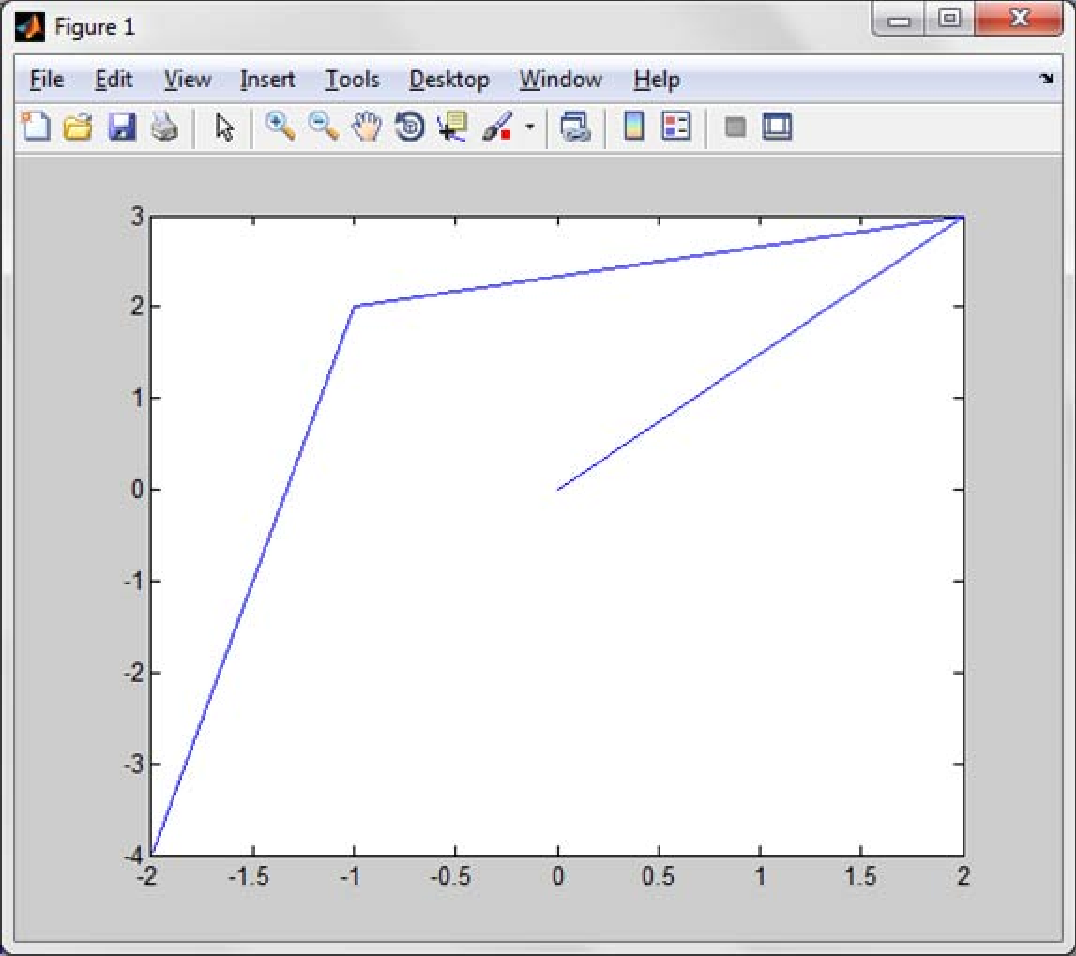
\includegraphics[width=12cm]{figura.pdf}
\caption{Ventana gráfica de Matlab. representación de los punto de la tabla \ref{tpuntos}}
\label{fig:ventana}
\end{figure}

La ventana gráfica de Matlab, tiene en su parte superior una barra de herramientas y un menú desplegable con funciones específicas para la manipulación de los gráficos. Se aconseja leer la ayuda de Matlab sobre el uso de dichas herramientas.

Una de las opciones del menú desplegable, permite guardar la figura generada como un archivo gráfico. Además, es posible mediante otra de las opciones del menú copiar la figura y pegarla posteriormente en un editor de texto\footnote{Al menos es posible hacerlo así si se trabaja en el sistema operativo Windows de Microsoft.}. Si copiamos la figura \ref{fig:ventana} y la pegamos directamente en el texto obtendríamos un gráfico como el de la figura, \ref{fig:plot}. A partir de ahora importaremos de esta manera todas las figuras que construyamos con Matlab.

\begin{figure}[h]
\centering
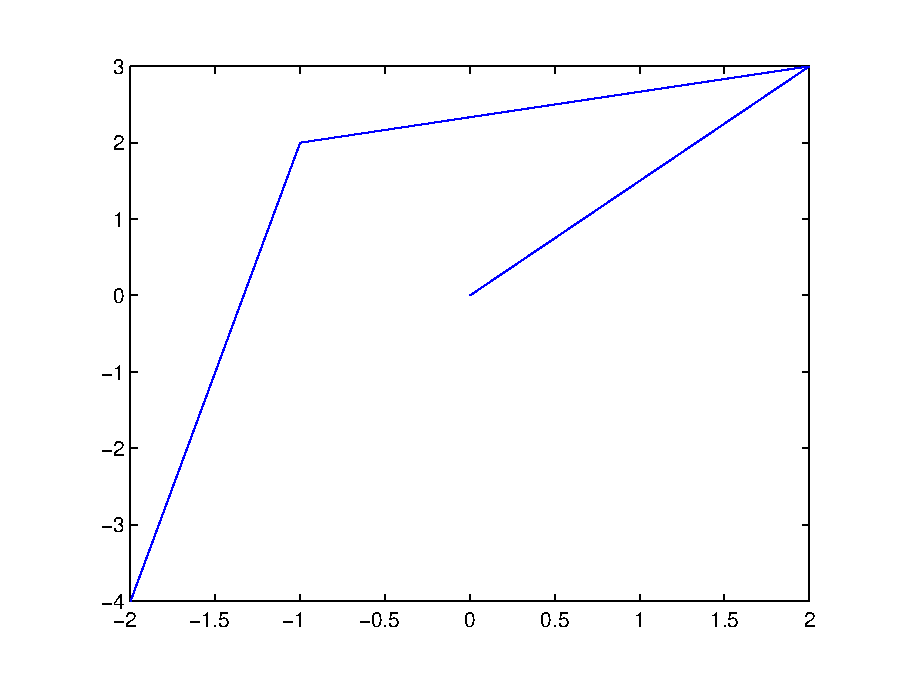
\includegraphics[width=12cm]{plot.eps}
\caption{gráfico de los puntos de la tabla \ref{tpuntos} obtenida con el comando \texttt{plot}}
\label{fig:plot}
\end{figure}
El comando plot admite un tercer parámetro de entrada. Se trata de símbolos, escritos entre comillas simples, que permiten definir: 
\begin{itemize}
\item El tipo de línea que se empleará en el gráfico. por ejemplo \texttt{plot(x,y,'-.`')} une los puntos mediante una línea de puntos y guiones.
\item El símbolo que se empleará para representar los puntos. Por ejemplo, \texttt{plot(x,y,'o')} dibuja un círculo en la posición de cada punto y no los une entre sí mediante líneas rectas.
\item El color que se empleará para dibujar. Por ejemplo, \texttt{plot(x,y,'r')}. Dibuja la gráfica en color rojo.
\end{itemize}

Si no se define este tercer parámetro, \texttt{plot} dibujará los gráficos, por defecto, en color azul, uniendo los puntos con líneas continuas y no usará ningún símbolo para dibujar los puntos individuales.
 
La tabla \ref{tcolor} muestra los símbolos disponibles para dibujar con el comando \texttt{plot}.

\begin{table}[h]
\caption{tipos de línea y color del comando \texttt{plot}}
\centering
\begin{tabular}{rc|rc|rc}
Tipo de línea&Símbolo&Tipo de punto& Símbolo &Color&Símbolo\\ 
\hline
continua&-&punto&.&azul&b\\
puntos&:&círculo&o&verde&g\\
puntos y guiones&-.&equis&x&rojo&r\\
guiones&--&más&+&cyan&c\\
&&asterisco&*&amarillo&y\\
&&diamante&d&negro&k\\
&&triangulo vértice abajo&v&blanco&w\\
&&triangulo vértice arriba&\^{}&&\\
&&triangulo vértice izquierda&\textless&&\\
&&triangulo vértice derecha&\textgreater&&\\
&&triangulo vértice arriba&\^{}&&\\
&&cuadrado&s&&\\
&&pentágono&p&&\\
&&hexágono&h&\\
\hline
\end{tabular}
\label{tcolor}
\end{table} 

Se puede combinar un símbolo de cada tipo en un mismo \texttt{plot}. Así por ejemplo si queremos representar los datos de la tabla \ref{tpuntos} unidos mediante una línea de puntos,
\begin{verbatim}
plot(x,y,':')
\end{verbatim} 

Si queremos que pinte solo los puntos sin unirlos con líneas y en color rojo,
\begin{verbatim}
plot(x,y,'.r')
\end{verbatim}

Si queremos que pinte los puntos representados por triángulos con el vértice hacia arriba, unidos mediante una línea continua y en color negro,

\begin{verbatim}
plot(x,y,'-^k')
\end{verbatim}

La figura \ref{fig:tplot} muestra los resultados de las combinaciones de símbolos que acabamos de describir.

\begin{figure}[h]
\centering
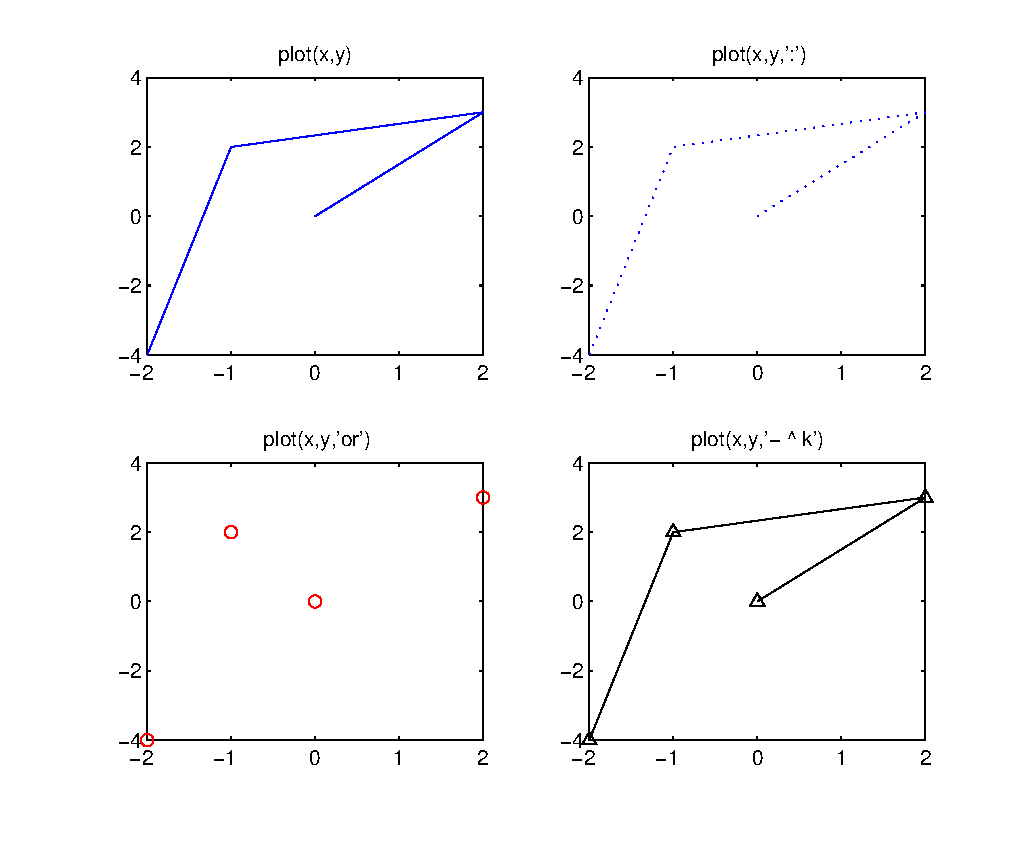
\includegraphics[width=12cm]{tiposplot.eps}
\caption{Datos de la tabla \ref{tpuntos} representados mediante distintos tipos de líneas y colores}
\label{fig:tplot}
\end{figure}

\paragraph{Figuras.} Cada vez que escribimos en la ventana de comandos de Matlab, un comando gráfico como por ejemplo \texttt{plot} Matlab comprueba si existe alguna figura (ventana de gráficos) abierta. Pueden darse entonces tres situaciones distintas. 

\begin{enumerate}
\item No hay ninguna figura abierta. Matlab crea entonces una figura nueva y representa en ella el gráfico pedido.
\item Hay una figura abierta. Matlab empleará dicha figura para representa el gráfico pedido. Por defecto, Matlab borrará cualquier gráfico anterior que contuviese la figura.
\item Existe más de una figura abierta. Matlab empleará para dibujar la llamada figura activa, que corresponde con la figura que se haya utilizado o que se haya seleccionado por última vez con el ratón.
\end{enumerate}

Es posible crear varias figuras distintas empleando directamente el comando \texttt{figure}. Cada vez que lo introduzcamos en la ventana de comandos, Matlab creará una figura nueva asignándole un número (figura 1, 2 ,3 etc.). Si empleamos el comando \texttt{figure}, seguido de un número entre paréntesis, \texttt{figure(25)}, Matlab creará una nueva figura asignándole dicho número y si ya existe la figura la convertirá en la figura activa.
El siguiente script muestra un ejemplo del uso de \texttt{figure} y \texttt{plot} combinados.

\begin{verbatim}
%este script  (figuras.m)muestra el uso de los comandos figure y plot para pintar
%varias funciones se aconseja copiarlo y probarlo en Matlab para entender
%mejor cómo funciona.

%vamos a pintar un trozo de la función e^x, en concreto para el intervalo
%x=[0,1]

%Construimos un vector de 100 puntos equiespaciados en el intervalo [0,1]

x=linspace(0,1,100);

%calculamos el valor de la funcion e^x para los puntos construidos,

y1=exp(x);

%pintamos los puntos y frente a x,

plot(x,y1) %plot ha construido una figura en Matlab, la figura 1.

%Construimos una segunda figura en Matlab
figure %se ha construido la figura 2

%construimos una tercera figura 
figure %se ha construido la figura 3


%calculamos los valores que tomará la función sin(2*pi*x) para los puntos
%x del intervalo [0,1] que ya tenemos
y2=sin(2*pi*x);

%hacemos activa la figura 2
figure(2)
%pintamos en esta figura los puntos de la función sin...

plot(x,y2)

%volvemos a hacer activa la figura 1
figure(1)
%pintamos ahora los puntos de la de la función y=e^x, pero invertidos x
%frente a y, La grafica anterior se borra y es sustituida por la nueva,
plot(y1,x)

%creamos una nueva figura asignándole un numero al crearla,
figure(13)

%volvemos activar la figura 3
figure(3)

%volvemos a pintar, ahora en la figura 3, la función y=e^x,
plot(x,y1)

%volvemos a activar la figura 13 y pintamos en ella de nuevo la funcion
%sin..

figure(13)
plot(x,y2)
\end{verbatim}

Como se ha señalado antes, cualquier comando gráfico que se ejecute borra por defecto el contenido anterior de la figura activa. Es posible cambiar este comportamiento, empleando para ello el comando \texttt{hold}. Si en la ventana de comandos escribimos \texttt{hold on}, a partir de ese momento la ventana activa mantendrá cualquier gráfico que contenga y añadirá a este los nuevos gráficos que se creen. Este comportamiento se mantiene hasta que vuelva a escribirse en la ventana de comandos la sentencia \texttt{hold off}. El siguiente script muestra un ejemplo del uso de este comando y La figura \ref{fig:sico} el gráfico resultante.

\begin{verbatim}
%ejemplo de uso de hold on para representar dos funciones en el mismo
%gráfico

%vamos a representar las funciones seno y coseno en el intervalo [-pi, pi]

%creamos un vector de 100 puntos en el intervalo,
x=[-pi:2*pi/99:pi];

%calculamos el valor de la función seno sobre los puntos x
seno=sin(x);

%calculamos el valor de la función coseno sobre los puntos x
coseno=cos(x);

%pintamos la funcion seno, con linea continua azul
plot(x,seno)

%le pedimos que mantenga el gráfico creado
hold on

%pintamos encima la función coseno en linea continua roja

plot(x,coseno,'r')

\end{verbatim}


\begin{figure}[h]
\centering
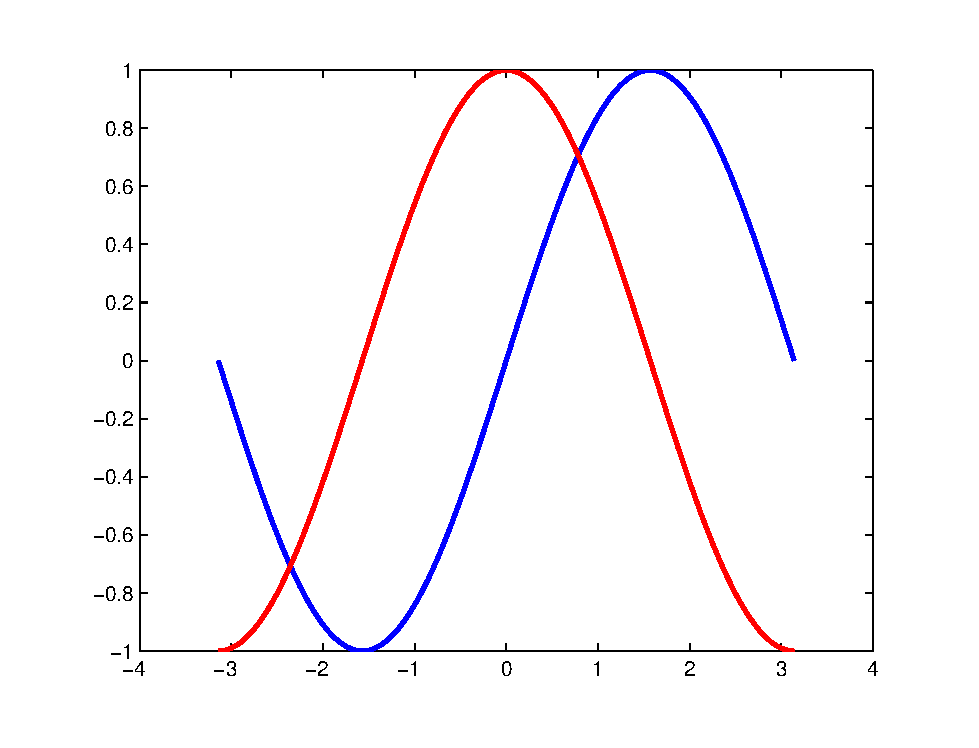
\includegraphics[width=12cm]{sico.eps}
\caption{gráficas de las funciones seno y coseno en el intervalo $(-\pi, \pi)$. Representadas en la misma figura, usando el comando \texttt{hold on}.}
\label{fig:sico}
\end{figure}

Es posible también incluir varios gráficos separados en la misma figura. 
Para ello se emplea el comando \texttt{subplot(i,j,k)}. Este comando divide la figura en un total de $i\times j$ gráficos y activa el situado en la posición $k$, las posiciones se cuentan fila a fila de arriba a abajo. El siguiente script muestra el uso del comando \texttt{suplot} La figura \ref{fig:subplot} muestra el resultado obtenido.


\begin{verbatim}
%Este script muestra el uso del comando subplot

%vamos a crear una figura con 2X3=6 gráficas, se disponen en la figura como
%si fueran los elementos de una matriz...
%usamos el comando subplot de modo que cree el primer eje de los 6
subplot(2,3,1)

%definimos un vector x de puntos equiespacios en el intervalo (-1,1)
x=linspace(-1,1,20);

%calculamos los valores de polinomio 3x^2+2^x-1
y=3*x.^2+2*x-1;

%dibujamos la función en los ejes
plot(x,y)

%Añadimos rótulos a los ejes
xlabel('eje x')
ylabel('eje y')
%Añadimos un titulo al grafico
title('gráfico 1')

%Generamos los siguientes ejes (a la derecha del anterior)
subplot(2,3,2)
%dibujamos la misma función pero ahora en linea discontinua roja
plot(x,y,':r')

%Añadimos rótulos a los ejes
xlabel('eje x')
ylabel('eje y')
%Añadimos un titulo al grafico
title('gráfico 2')

%Generamos los siguientes ejes (a la derecha del anterior)
subplot(2,3,3)
%dibujamos la misma función pero ahora en linea de punto y raya negra
plot(x,y,'-.k')

%Añadimos rótulos a los ejes
xlabel('eje x')
ylabel('eje y')
%Añadimos un titulo al grafico
title('gráfico 3')

%Generamos los siguientes ejes (debajo de los primeros)
subplot(2,3,4)
%dibujamos la misma función pero ahora solo con circulos azules
plot(x,y,'o')

%Añadimos rótulos a los ejes
xlabel('eje x')
ylabel('eje y')
%Añadimos un titulo al grafico
title('gráfico 4')

%Generamos los siguientes ejes (a la derecha del anterior)
subplot(2,3,5)
%dibujamos la misma función pero ahora solo con cruce rojas
plot(x,y,'+r')

%Añadimos rótulos a los ejes
xlabel('eje x')
ylabel('eje y')
%Añadimos un titulo al grafico
title('gráfico 5')

%Generamos los últimos ejes (a la derecha del anterior)
subplot(2,3,6)
%dibujamos la misma función pero ahora en linea continua y asteriscos
%negros
plot(x,y,'-*k')

%Añadimos rótulos a los ejes
xlabel('eje x')
ylabel('eje y')
%Añadimos un titulo al grafico
title('gráfico 6')
\end{verbatim}

\begin{figure}[h]
\centering
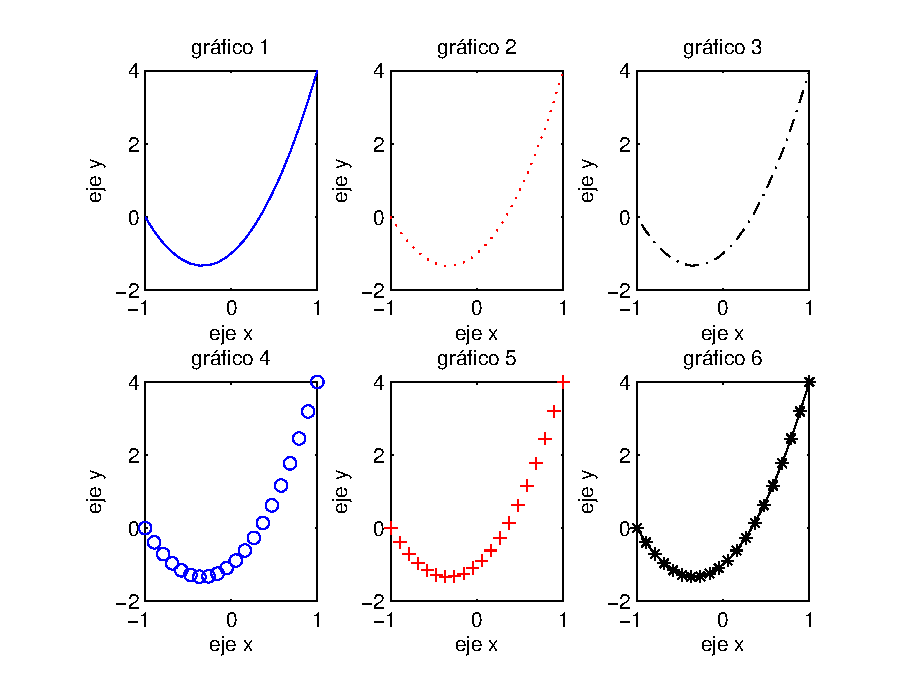
\includegraphics[width=12cm]{subplot.eps}
\caption{Ejemplo de empleo del comando subplot}
\label{fig:subplot}
\end{figure}

En el ejemplo, se ha hecho usos de algunos comandos para gráficos que permiten introducir títulos. Estos son: 

\texttt{title}, introduce un titulo a un gráfico, por ejemplo,
\begin{verbatim}
title('gráfico de temperaturas')
\end{verbatim}

\texttt{xlabel}, añade un rótulo al eje x, por ejemplo,

\begin{verbatim}
xlabel('tiempo en segundos')
\end{verbatim}

\texttt{ylabel} añade un rótulo al eje y , por ejemplo,
\begin{verbatim}
ylabel('distancia en metros')
\end{verbatim}

\subsection{Gráficos en 2D} \index{Gráficos! Comandos gráficos en 2D}
Hasta ahora, hemos visto tan solo el comando \texttt{plot}, que nos ha servido para introducir las capacidades gráficas en Matlab. Como hemos visto, plot permite representar gráficamente colecciones de datos en dos dimensiones. Hay otros muchos comandos que permiten obtener representaciones \emph{especializadas} de datos en dos dimensiones. A continuación veremos algunos de los más destacables.

\paragraph{fplot.} Permite dibujar directamente una función en un intervalo de valores. El nombre de la función hay que introducirlo entre comillas simples y el intervalo como un vector de dos componentes. Por ejemplo,

\begin{verbatim}
>> fplot('exp(-x.^2).*cos(6*pi*x)',[-3 3])
\end{verbatim}

dibuja la función,
\begin{equation*}
f(x)=e^{-x^2}\cos(6\pi x)
\end{equation*}

en el intervalo $[-3,3]$ (figura \ref{fig:wave}.

\begin{figure}[h]
\centering
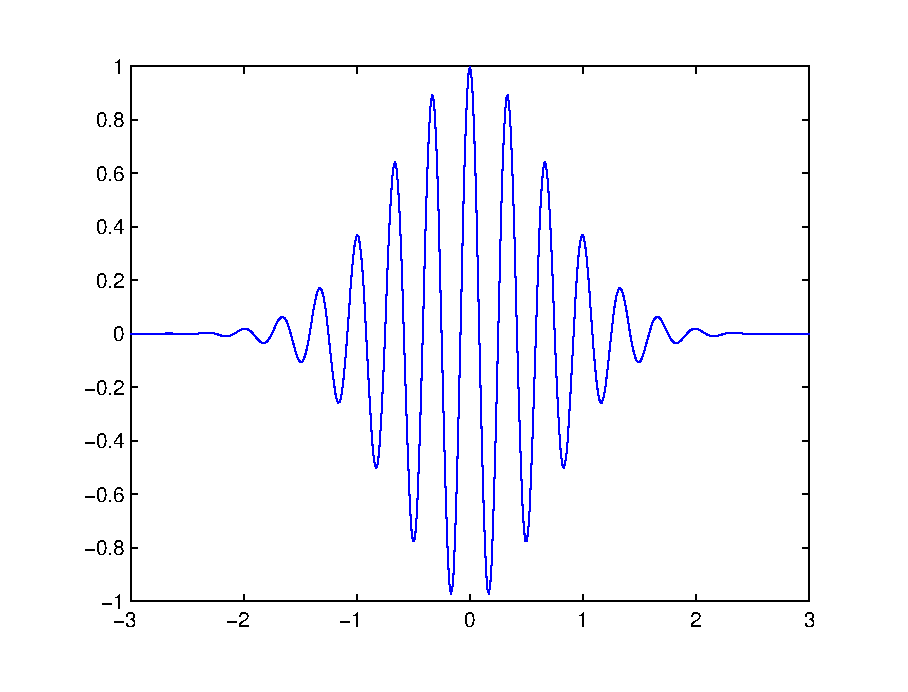
\includegraphics[width=12cm]{wave.eps}
\caption{Ejemplo de empleo del comando \texttt{fplot}}
\label{fig:wave}
\end{figure} 
 
\paragraph{semilogx.} El comando \texttt{semilog} representa el eje de las x en escala logarítmica, Es decir, en lugar de representar frente a la variable $x$, se representa frente a $\log_{10}(x)$. Si dibujamos empleando este tipo de gráfico la función $y=\log_{10}(x)$ deberíamos obtener una línear recta de pendiente unidad. La figura \ref{fig:slx} muestra el resultado, empleando para las \emph{equis} el intervalo $(0,1)$.
\begin{verbatim}
>> x=linspace(0,1,100);
>> y=log10(x);
>> semilogx(x,y)
>> grid on
\end{verbatim}

\begin{figure}[h]
\centering
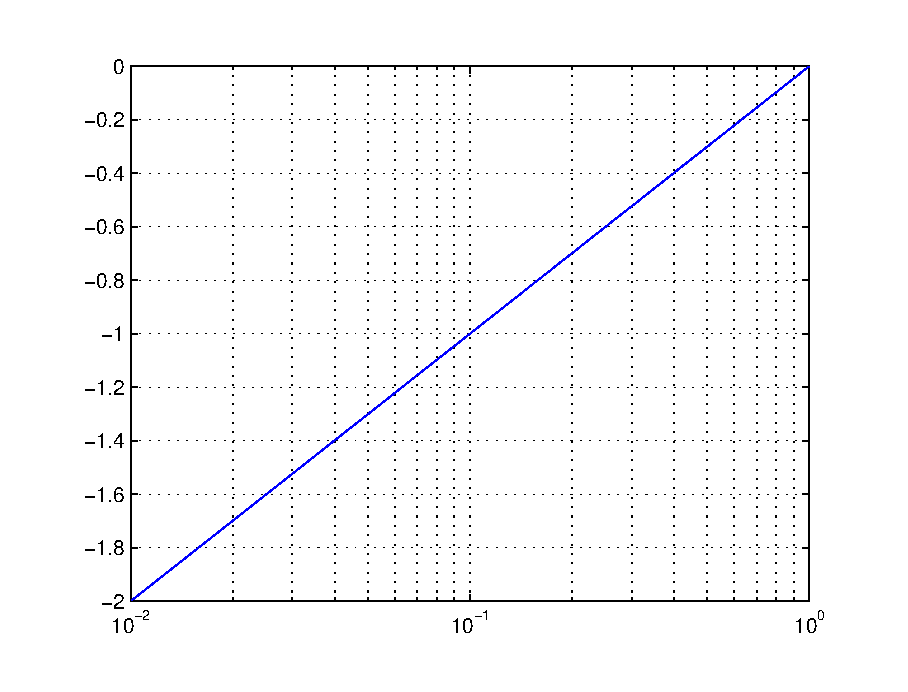
\includegraphics[width=10cm]{slx.eps}
\caption{Representación de la función $y=\log_{10}(x)$ empleando el comando \texttt{semilogx}}
\label{fig:slx}
\end{figure} 

Un par de observaciones sobre este ejemplo: En primer lugar las divisiones del eje x aparecen marcadas como potencias de 10. Como estamos representando empleando el logaritmo decimal de la variable x, las divisiones se corresponden con el exponente de la potencia de 10 de cada división, $\log_{10}(10^n)=n$.

En segundo lugar hemos empleado un nuevo comando gráfico; se trata del comando \texttt{grid}. Este comando añade una retícula al gráfico de modo que sea más fácil ver los valores que toman las variables en cada punto de la gráfica. \texttt{grid on},añade la retícula y \texttt{grid off} la retira.

\paragraph{semilogy.} Análoga al anterior, simplemente que ahora es el eje y el que se representa en escala logarítmica. En este caso será si representamos la función $y=10^x$ cuando obtengamos una línea recta,

\begin{verbatim}
>> x=linspace(0,1,100);
>> y=10.^x;
>> semilogy(x,y)
>> grid on
\end{verbatim}

\begin{figure}[h]
\centering
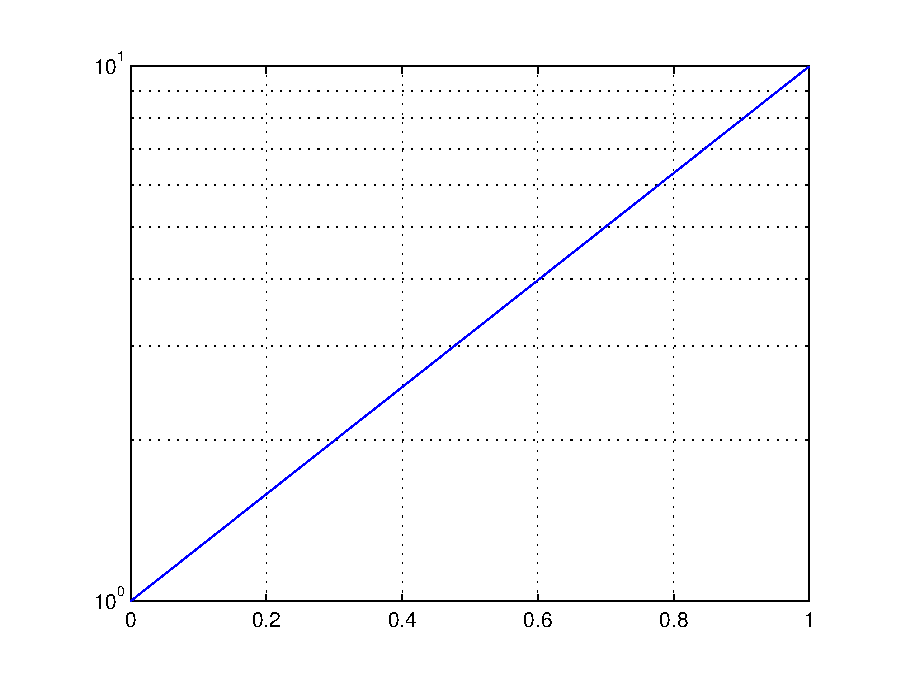
\includegraphics[width=10cm]{sly.eps}
\caption{Representación de la función $y=10^x$ empleando el comando \texttt{semilogy}}
\label{fig:sly}
\end{figure}

\paragraph{loglog.} Análoga a las anteriores, \texttt{loglog(x,y)} representa \texttt{y} frente a \texttt{x} empleando en ambos ejes una escala logarítmica.


\paragraph{polar.} Representa funciones en coordenadas polares \texttt{polar(theta,r}. La primera variable es un ángulo en radianes y la segunda el correspondiente radio. La figura \ref{fig:esp} muestra la espiral,
\begin{equation*}
r=2\cdot\sqrt{\theta}
\end{equation*}

Para el intervalo angular $[0,8\pi]$.
 
\begin{verbatim}
>> theta=linspace(0,8*pi,100);
>> r=2*theta;
>> polar(theta,r)
>> r=sqrt(theta);
>> polar(theta,r)
\end{verbatim}

\begin{figure}[h]
\centering
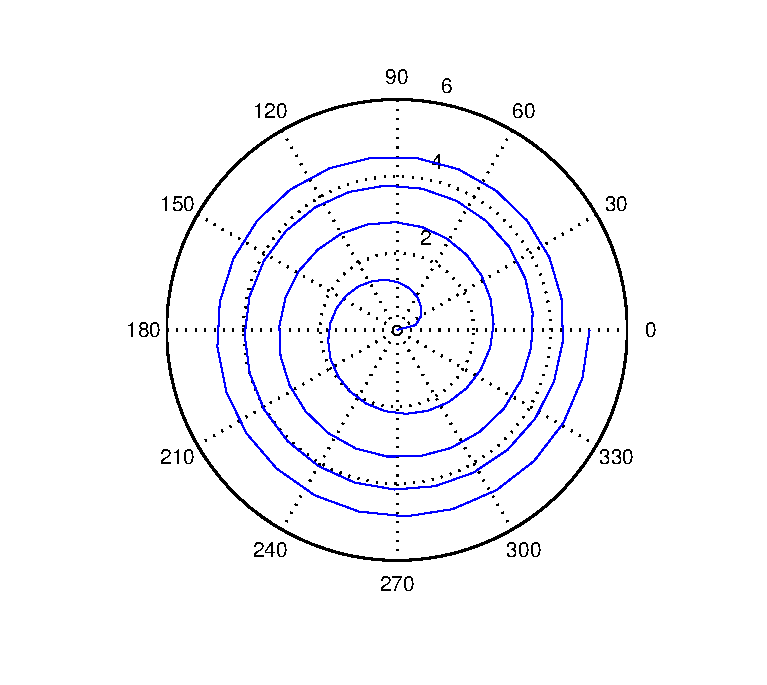
\includegraphics[width=10cm]{esp.eps}
\caption{Representación de la función $r=\sqrt{\theta}$ empleando el comando \texttt{polar}}
\label{fig:esp}
\end{figure}

\paragraph{stem, bar, stairs.} En los tres casos, se obtienen representaciones \emph{discretas} de un conjunto de datos. \texttt{stem} representa los datos mediante líneas verticales que parten del eje  x y llegan hasta el valor correspondiente de y. Las líneas van rematadas por un círculo. \texttt{bar} Emplea barras solidas verticales  y \texttt{stairs} realiza una representación en escalera. La figura \ref{fig:sbs} muestra el resultado de dibujar, empleando estos tres tipos de gráficos, los datos correspondientes al número de coches por cada 1000 habitantes en 2007 para cincuenta países distintos (los datos se guardaban en una matriz llamada auto\_50\_2007),

\begin{verbatim}
>> subplot(1,3,1)
>> stem(auto_50_2007)
>> subplot(1,3,2)
>> bar(auto_50_2007)
>> subplot(1,3,3)
>> stairs(auto_50_2007)
\end{verbatim}

\begin{figure}[h]
\centering
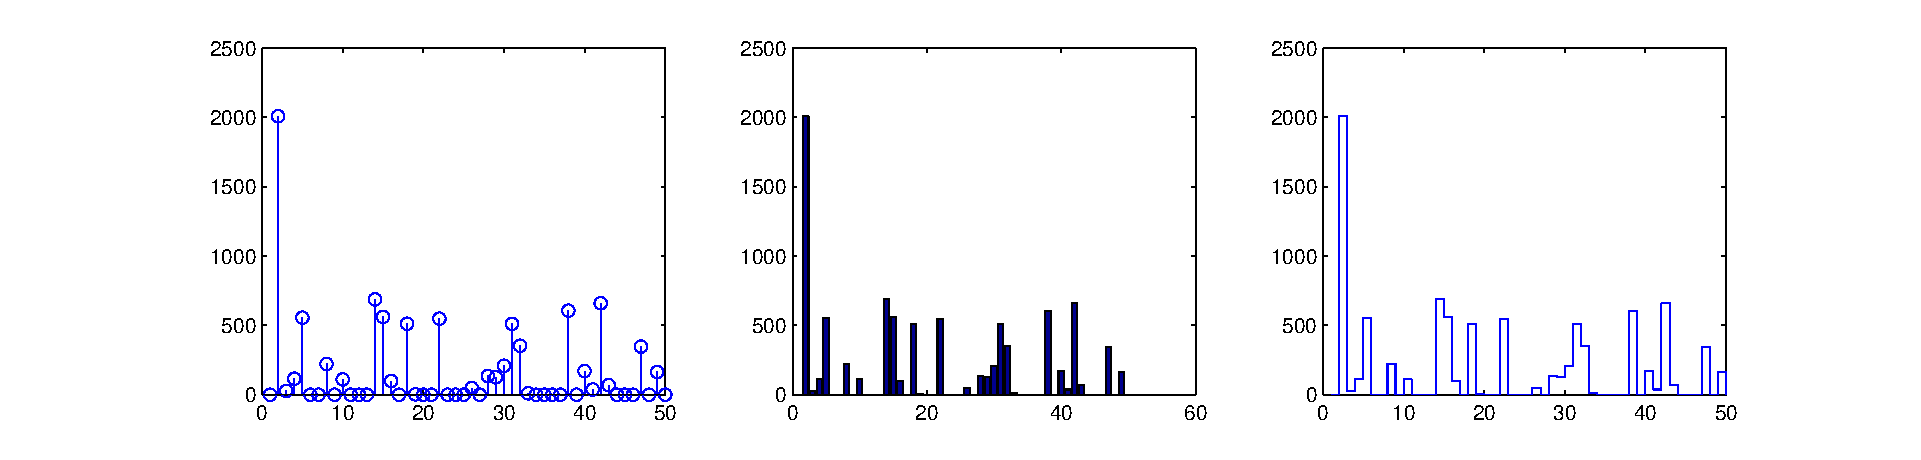
\includegraphics[width=15cm]{sbs.eps}
\caption{Comparción entre los comandos \texttt{stem}, \texttt{bar} y \texttt{stairs} representando la misma colección de datos.}
\label{fig:sbs}
\end{figure}

\paragraph{hist.} Este comando permite dibujar el histograma de una colección de datos. El histograma es una forma de representar cuantas veces se repite un datos, o más exactamente cuantos datos de la colección caen dentro de un intervalo dado. La función \texttt{hist(x,n)} admite dos parámetros de entrada, un vector de datos \texttt{x} y un valor entero \texttt{n} que representa el número de intervalos en que se dividirá el rango de valores de \texttt{x}, para obtener el histograma. Si no se introduce esta segunda variable, Matlab por defecto divide el rango de los datos en 10 intervalos. Veamos un ejemplo de uso de hist, empleando los datos del ejemplo anterior relativos a número de coches por cada mil habitantes. Representaremos el histograma para un total de 213 países. Para tener una idea, del rango de los dato, calculamos el valor mínimo y máximo de los datos disponibles,
\begin{verbatim}
>> minimo=min(auto2007)
minimo =

     0

>> maximo=max(auto2007)

maximo =

   874
\end{verbatim}

El rango va de $0$ a $879$ automóviles por cada mil habitantes. La figura \ref{fig:hist} muestra los histogramas obtenidos sin indicar el número de intervalos, ---por lo que se tomarán 10---, tomando 5 intervalos y tomando 20.

\begin{verbatim}
>> subplot(1,3,1)
>> hist(auto2007)
>> subplot(1,3,2)
>> hist(auto2007,5)
>> subplot(1,3,3)
>> hist(auto2007,20)
>> subplot(1,3,1)
>> title('10 intervalos')
>> subplot(1,3,2)
>> title('5 intervalos')
>> subplot(1,3,3)
>> title('20 intervalos')
\end{verbatim}

\begin{figure}[h]
\centering
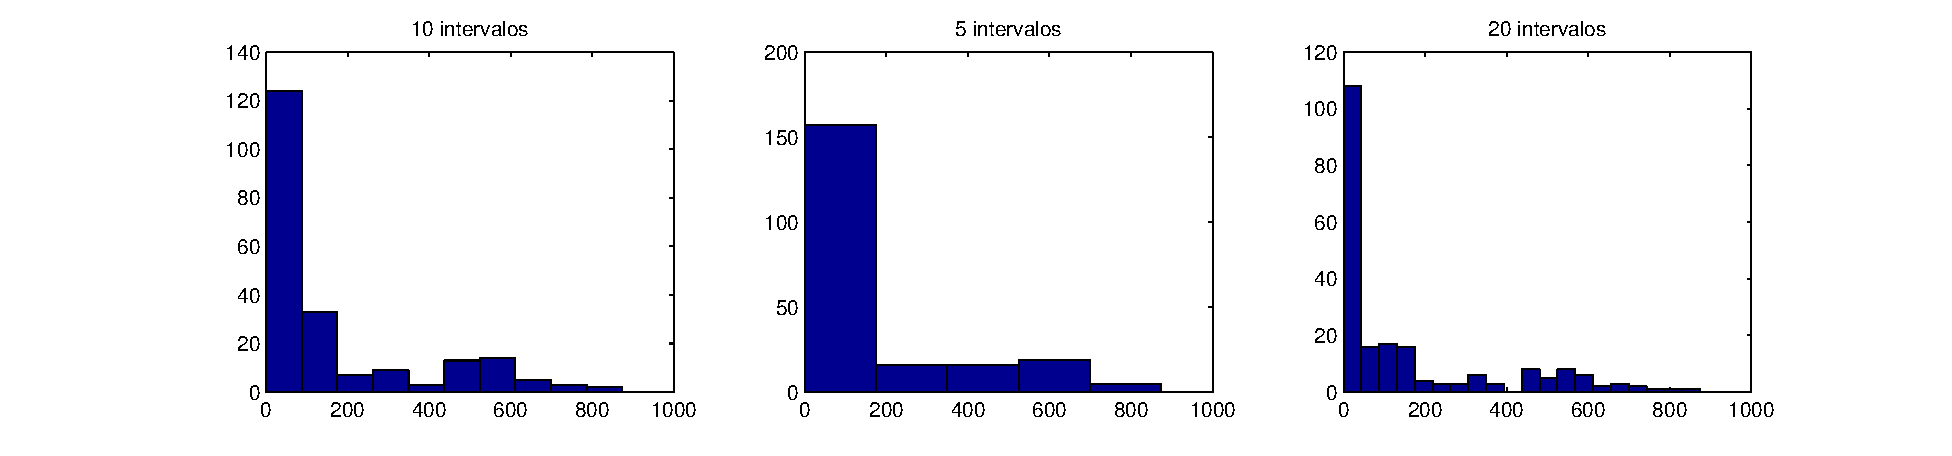
\includegraphics[width=15cm]{hist.eps}
\caption{histogramas del número de automóviles por cada 1000 habitantes para 213 países}
\label{fig:hist}
\end{figure}

La interpretación del los histogramas depende lógicamente del número de intervalos. En el caso de 10 intervalos, estos dividen los datos en grupos de aproximadamente 100 coches. Si observamos el histograma resultante, podemos concluir que hay unos 120 países en los que hay entre 0 y 100 automóviles por cada 1000 habitante, unos 30 países en los que hay entre 100 y 200 automóviles por cada 1000 habitante, etc. Si miramos el siguiente histograma, en el que se han empleado tan solo 5 intervalos, los grupos son ahora de aproximadamente 200 coches. La primera barra de este segundo histograma establece que hay unos 150 países en los que hay entre 0 y 200 coches por cada 1000 habitantes. Resultado que corresponde a la suma de los de dos primeros intervalos del histograma anterior. Para el tercer histograma los intervalos son ahora de 50 automóviles, lo que permite observar más en detalle que en los histogramas anteriores la distribución de vehículos: 110 países tienen menos de 50 automóviles por cada 1000 habitantes.

\paragraph{plotyy.} Este comando permite representar dos gráficas en la misma figura de modo que comparten el mismo eje x y cada una tiene su propio eje y. La figura \ref{fig:plotyy} muestra el resultado del siguiente ejemplo,

\begin{verbatim}
>> x1=linspace(0,10,100);
>> x2=linspace(0,12,50);
>> y1=x1.^2;
>> y2=x2.^(2/3);
>> plotyy(x1,y1,x2,y2)
>> grid on
\end{verbatim}

\begin{figure}[h]
\centering
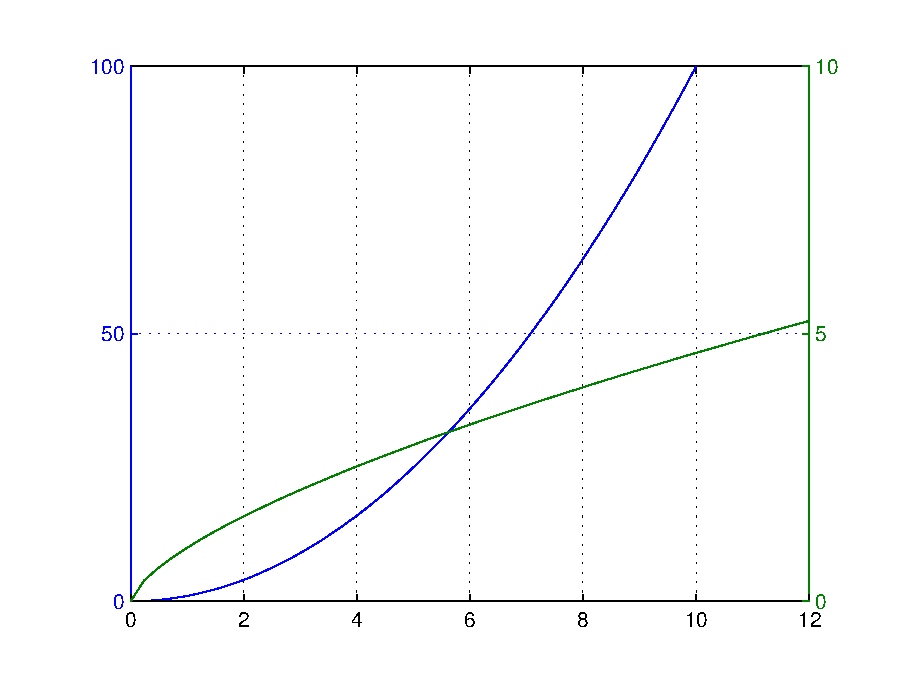
\includegraphics[width=10cm]{plotyy.eps}
\caption{Ejemplo de uso de la función \texttt{plotyy}}
\label{fig:plotyy}
\end{figure}

\paragraph{quiver.} Esta función de Matlab permite dibujar vectores en el plano. En realidad está pensada para dibujar campos vectoriales, con lo que hay que manejarla con cierto cuidado. En primera aproximación diremos que \texttt{quiver} necesita 5 variables de entrada: la coordenada $x$ del origen del vector, la coordenada $y$ del origen del vector, la componente $x$ del vector y la componente $y$ del vector, por último, un factor de escala al que daremos el valor $0$ para que dibuje los vectores a su tamaño real, sin modificar su escala. Por ejemplo si queremos dibujar el vector $\vec{v}=(1,2)$ situado en el origen de coordenadas,
\begin{verbatim}
quiver(0,0,1,2,0)
\end{verbatim}

Si queremos representar el mismo vector pero situado en el punto $(3,-1)$,
\begin{verbatim}
>>quiver(3,-1,1,2,0)
\end{verbatim}

Podemos dibujar un conjunto de vectores con quiver, para ello empleamos como variables de entradas vectores, en lugar de escalares; un vector que contenga las posiciones $x$ del los orígenes, un segundo vector que contenga la posiciones $y$ de los orígenes, un tercer vector que contenga las componentes $x$ de los vectores y un cuarto que contenga las componentes $y$, por último añadiríamos el parámetro de escala $0$, que sigue siendo un escalar.

Por tanto, si queremos dibujar a la vez los dos vectores de los ejemplos anteriores,

\begin{verbatim}
>>quiver([0 3],[0 -1],[1 1],[2 2],0)
\end{verbatim}

La figura \ref{fig:quiver} muestra los resultados del ejemplo que acabamos de ver,

\begin{figure}[h]
\centering
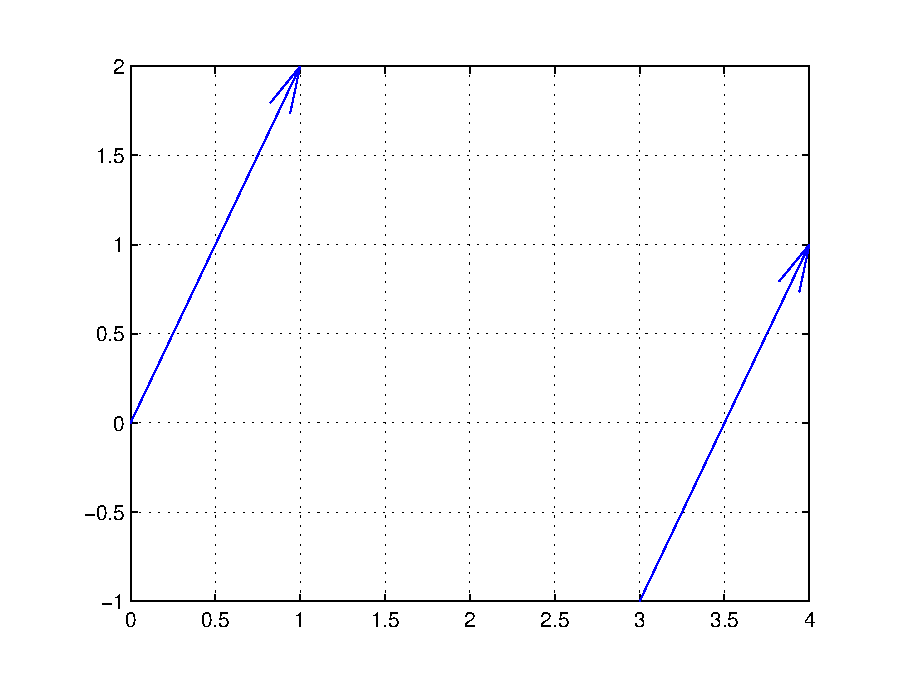
\includegraphics[width=10cm]{quiver.eps}
\caption{Ejemplo de uso de la función \texttt{quiver}}
\label{fig:quiver}
\end{figure}

\paragraph{errorbar.} Permite añadir barras de  error a un gráfico de puntos experimentales. Supongamos que tenemos la siguiente tabla (\ref{vel}) de resultados de la medida de la velocidad de un móvil frente al tiempo,


\begin{table}[h]
\caption{Resultados experimentales de la medida de la velocidad de un móvil}
\centering
\begin{tabular}{ccc}
\hline
\hline
tiempo &velocida& incertidumbre\\ 
$t$ (s)&$v$ (m/s)& $\pm \Delta v$ (m/s)\\
\hline
0&0&0\\
1&2.8&0.8\\
2&4.0&0.8\\
3&4.3&0.9\\
4&4.2&0.9\\
5&4.8&1.0\\
6&6.3&1.0\\
7&7.9&1.0\\
8&8.9&1.1\\
9&9.0&1.1\\
10&8.7&1.1\\
\hline
\hline
\end{tabular}
\label{vel}
\end{table} 

La primera columna representa el instante de tiempo en que se tomó la medida, la segunda columna representa el valor medido de la velocidad y la tercera columna la incertidumbre de cada medida de velocidad.

podemos emplear el comando \texttt(errorbar) para representar la velocidad frente al tiempo, añadiendo una barra de error en cada medida que represente la incertidumbre,

\begin{verbatim}
>> vel=[0 2.8 4.0 4.3 4.2 4.8 6.3 7.9 8.9 9.0 8.7]
vel =

  Columns 1 through 7

         0    2.8000    4.0000    4.3000    4.2000    4.8000    6.3000

  Columns 8 through 11

    7.9000    8.9000    9.0000    8.7000

>> inc=[0 0.8 0.8 0.9 0.9 1.0 1.0 1.0 1.1 1.1 1.1]
inc =

  Columns 1 through 7

         0    0.8000    0.8000    0.9000    0.9000    1.0000    1.0000

  Columns 8 through 11

    1.0000    1.1000    1.1000    1.1000

>> t=0:10
t =

     0     1     2     3     4     5     6     7     8     9    10

>> errorbar(t,vel,inc)
>> xlabel('tiempo s')
>> ylabel('velocidad m/s')
\end{verbatim}

EL resultado se muestra en la figura \ref{fig:error}. Es interesante hacer notar que la longitud total de cada barra de error es el doble del valor de la incertidumbre correspondiente al punto. Por ejemplo para $t=1s, v+\Delta v=2.8\pm 0.8 m/s$ la longitud de la barra de error es $2\cdot \Delta v=1.6 m/s$). El comando \texttt{errobar}, puede también emplearse para representar incertidumbres asimétricas. Para ello  es preciso suministrar dos vectores uno \texttt{U} para dibujar la parte superior de la barra de error y otro \texttt{L} para dibujar la parte inferior; \texttt{errorbar(x,y,L,U)}. 

\begin{figure}[h]
\centering
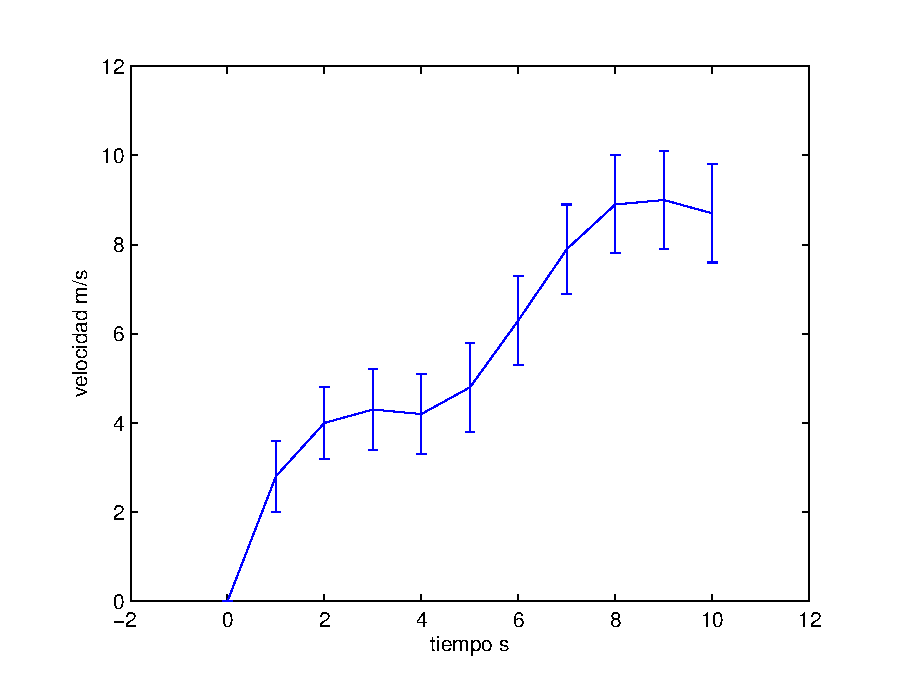
\includegraphics[width=11cm]{error.eps}
\caption{Datos de la tabla \ref{vel} representados empleando el comando \texttt{errorbar}}
\label{fig:error}
\end{figure}

\subsection{Gráficos en 3D.} \index{Gráficos! Comandos gráficos en 3D}En tres dimensiones es posible representar dos tipos de gráficos: puntos y curvas, análogos a los representados en dos dimensiones y además superficies en el espacio.

\paragraph{plot3.} Para dibujar líneas y puntos Matlab emplea los mismos comandos que hemos descrito para dos dimensiones, añadiendo al nombre de comando la terminación \texttt{3} para indicar que se trata de un gráfico en tres dimensiones. Así por ejemplo el comando \texttt{plot3} nos permite dibujar puntos y curvas en el espacio. El manejo es idéntico al de \texttt{plot}, simplemente que ahora es preciso añadir un vector que contenga los datos de la tercera coordenada, z. 

Por ejemplo, podemos representar la curva,
\begin{align*}
y&=\sin(2\pi x)\\
z&=\cos(2\pi x)
\end{align*}

Para ello, seleccionamos un intervalo de valores para $x \in (0,2)$, y calculamos los correspondientes valores de $y$ y $z$,

\begin{verbatim}
>> x=linspace(0,2,100);
>> y=sin(2*pi*x);
>> z=cos(2*pi*x);
\end{verbatim}

Podemos ahora representar la gráfica de nuestra función empleando el comando \texttt{plot3},
\begin{verbatim}
>> plot3(x,y,z)
>> grid on
>> xlabel('x')
>> ylabel('y')
>> zlabel('z')
\end{verbatim}

Hemos añadido los comandos \texttt{grid on}  para obtener una trama en 3D que permita ver mejor el resultado. La figura \ref{fig:muelle1} muestra la figura de Matlab obtenida, donde se ha señalado además un botón que permite rotar la figura, cambiando la vista. Para ellos, una vez pulsado el botón, basta con arrastrar el ratón sobre la figura manteniedo pulsado el boton izquierdo.  La figura \ref{fig:muelle2}, muestra la misma gráfica en 3D, pero ahora vista de frente (como si nos situáramos en el eje x). La figura \ref{fig:muelle3}, nos muestra la grafica vista desde arriba (desde el eje z), por último, la figura \ref{fig:muelle4} muestra una vista lateral de la gráfica (tomada desde el eje y).

Es posible rotar la figura par a obtener una vista concreta mediante el comando \texttt{view(Az, El)}. Este comando admite dos parámetros; \texttt{Az}, representa el azimuth o ángulo de rotación horizontal, \texttt{El}, representa el ángulo de elevación. Ambos ángulos se introducen en grados. Así, por ejemplo las vistas representadas en las figuras anteriores, se pueden obtener como,
\begin{verbatim}
>> view(90,0)
>> view(0,90)
>> view(0,0)
\end{verbatim}

\begin{figure}[h]
\centering
\subfigure[ventana gráfica \label{fig:muelle1}]{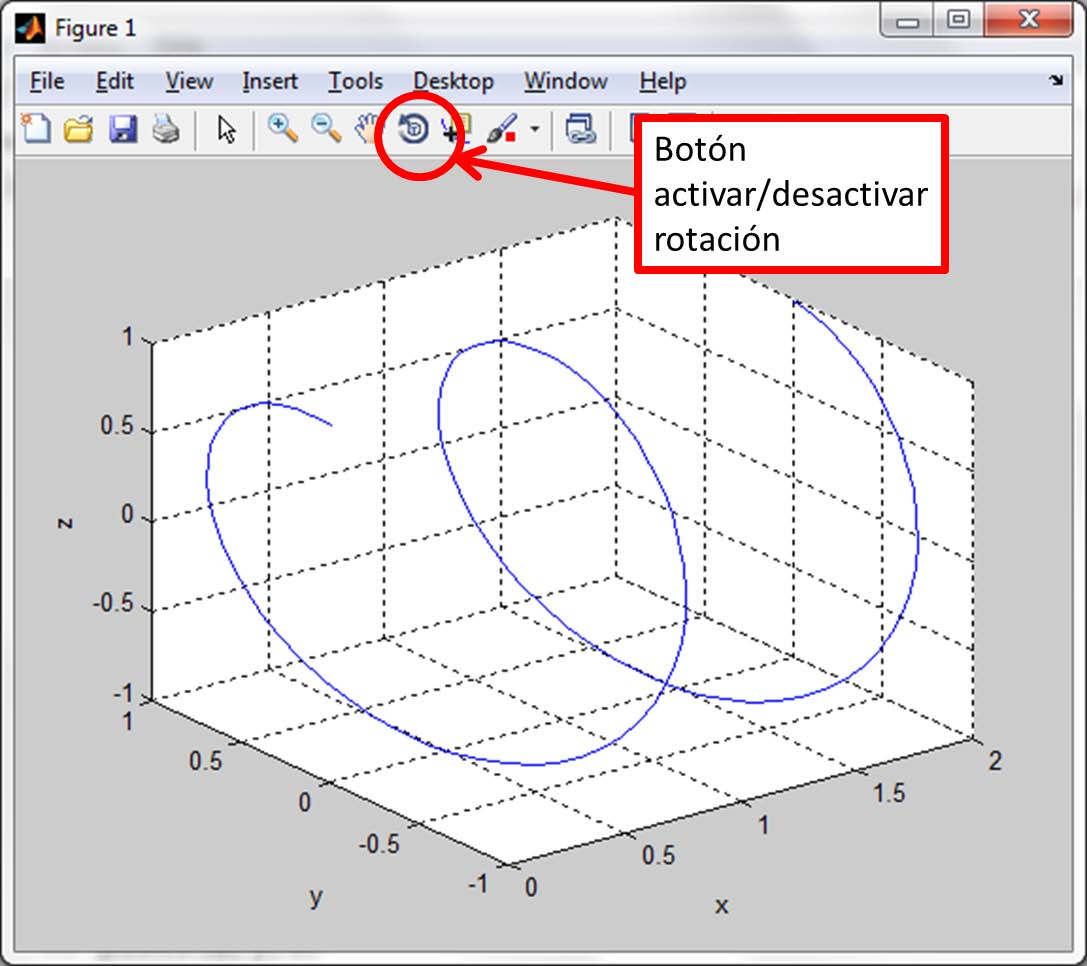
\includegraphics[width=6cm]{muelle1.pdf}} \qquad 
\subfigure[vista frontal (eje x) \label{fig:muelle2}]{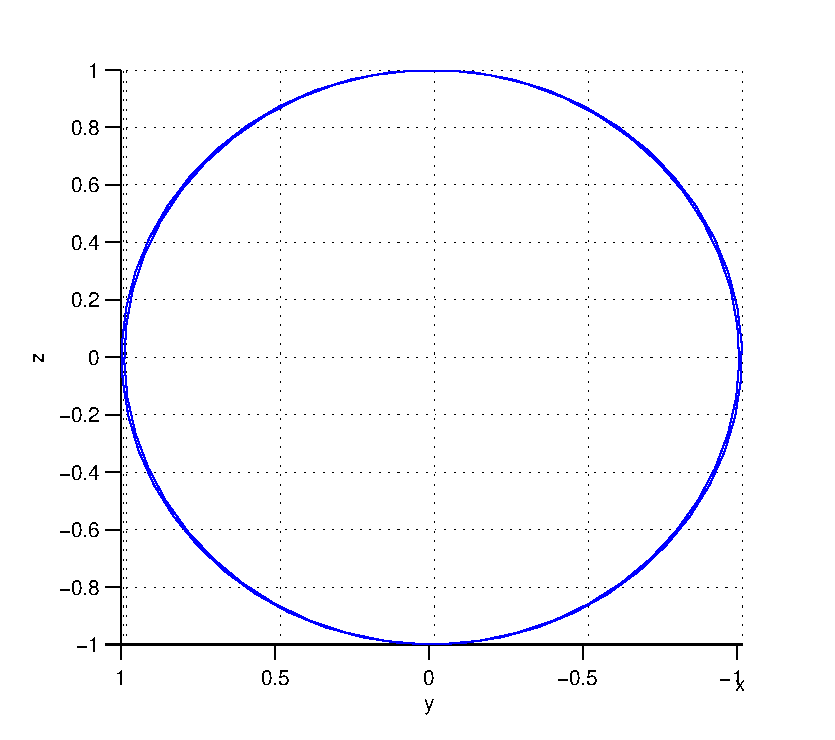
\includegraphics[width=6cm]{muelle2.eps}}\\
\subfigure[vista desde arriba (eje z) \label{fig:muelle3}]{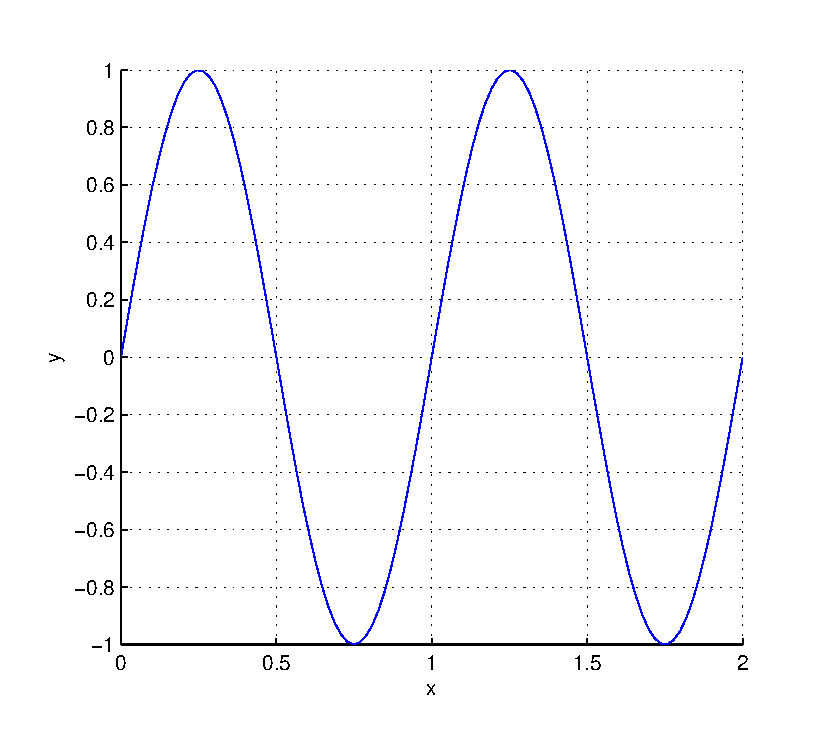
\includegraphics[width=6cm]{muelle3.eps}}\qquad
\subfigure[vista lateral (eje y)l \label{fig:muelle4}]{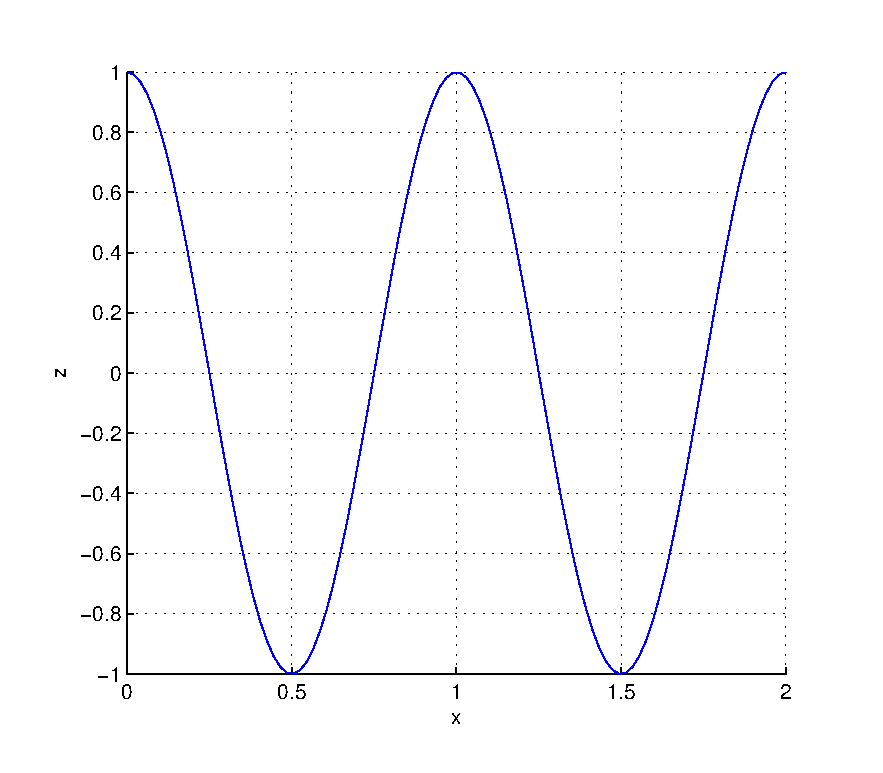
\includegraphics[width=6cm]{muelle4.eps}}\\
\caption{Gráfico en 3D y rotaciones. }
\end{figure}

\paragraph{bar3, stem3, hist3, quiver3.} Existen versiones 3D de los comandos \texttt{bar}, \texttt{stem}, \texttt{hist} y \texttt{quiver}. Su funcionamiento es similar ---aunque no siempre igual--- al de la versión 2D que vimos en la sección anterior. En algunos casos necesitan tres variables de entrada, correspondientes a las componentes (x,y,z) de los datos que se quiere representar, y en otros necesitan que los datos de entrada se le suministren en forma de matriz. Para conocer en detalle su funcinamiento, lo ideal es acudir a la ayuda de Matlab.


\paragraph{Superficies.}Para trazar superficies en el espacio, Matlab necesita en primer lugar que se defina una retícula en el plano $(x,y)$ que sirve de base sobre la que calcular los puntos z sobre los que se alzará la superficie.

Para definir dicha retícula Matlab emplea dos matrices. una de ellas $X_m$ contiene las coordenadas $x$ de los nodos de la retícula y la otra $Y_m$ las coordenadas $y$. Los elementos que ocupan la misma posición en ambas matrices, representan ---juntos--- un punto en el plano.
Matlab emplea dichas matrices como matrices de \emph{adyacencia}. Cada nodo, $(x_m(i,j),y_m(i,j)$, aparecerá en la gráfica conectado por una arista a cada uno de sus cuatros puntos vecinos, $(x_m(i-1,j),y_m(i-1,j)$, $(x_m(i,j-1),y_m(i,j-1)$, $(x_m(i+1,j),y_m(i+1,j)$, $(x_m(i,j+1),y_m(i,j+1)$.
Supongamos que empleamos las siguientes matrices, $X_m$ y $Y_m$ para definir una retícula sobre la que dibujar una superficie,

\begin{align*}
X_m=\begin{pmatrix}
0&1&2&3\\ 
0&1&2&3\\
0&1&2&3\\
0&1&2&3
\end{pmatrix},& Y_m\begin{pmatrix}
0&0&0&0\\
1&1&1&1\\
2&2&2&2\\
3&3&3&3
\end{pmatrix}\xrightarrow[nodos]{posiciones}\begin{matrix}
(0,0)&-&(1,0)&-&(2,0)&-&(3,0)\\
\vert&&\vert&&\vert&&\vert\\ 
(0,1)&-&(1,1)&-&(2,1)&-&(3,1)\\
\vert&&\vert&&\vert&&\vert\\
(0,2)&-&(1,2)&-&(2,2)&-&(3,2)\\
\vert&&\vert&&\vert&&\vert\\
(0,3)&-&(1,3)&-&(2,3)&-&(3,3)
\end{matrix}
\end{align*}

La retícula definida por Matlab, a partir de dichas matrices tendría el aspecto que se muestra en la figura \ref{fig:mesh}. 

\begin{figure}[h]
\centering
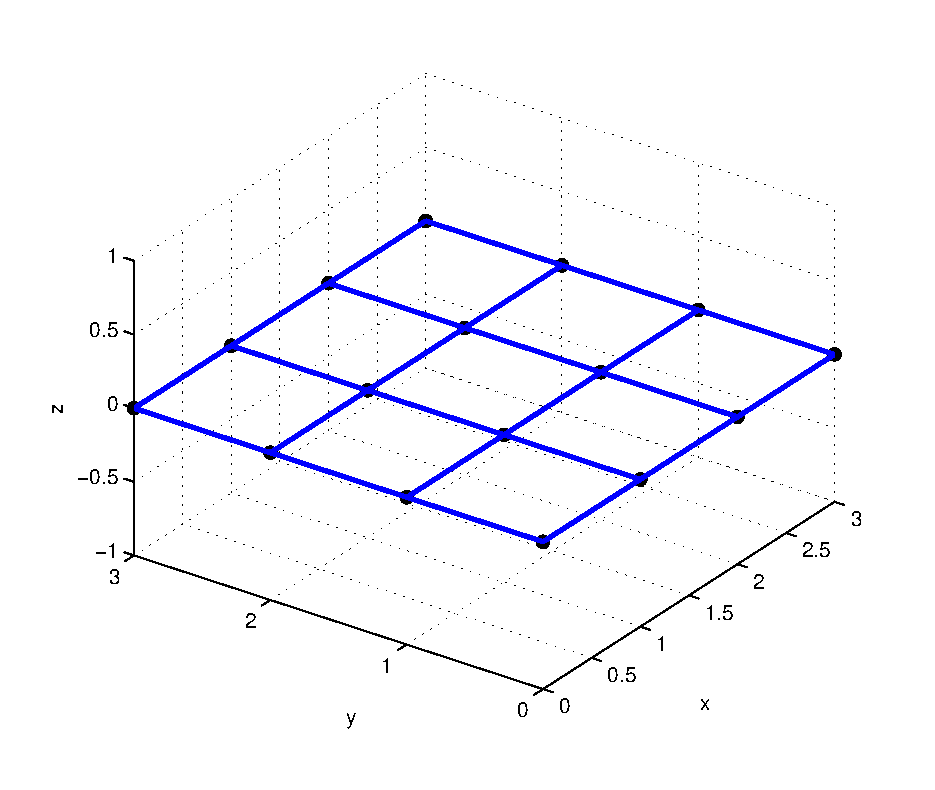
\includegraphics[width=11cm]{mesh.eps}
\caption{Retícula para representar superficies. Los puntos negros son los nodos definidos por las matrices $X_m$ e $Y_m$.}
\label{fig:mesh}
\end{figure}

Si nos fijamos en los ejes de la figura es fácil obtener las coordenadas de los nodos y comprobar como, están unidos entre sí por aristas los que ocupan posiciones adyacentes en las matrices $X_m$ e $Y_m$.

Para construir una superficie sobre la retícula, lo único que hace falta es definir una altura (z), para cada punto de la retícula. Para ello, Matlab emplea una matriz, del mismo tamaño que $X_m$ y $Y_m$. Así por ejemplo, si definimos,

\begin{equation*}
Z_m=\begin{pmatrix}
0&0&0&\\ 
0&1&2&0\\
0&3&4&0\\
0&0&0&0
\end{pmatrix}
\end{equation*}

Cada elemento de la matriz $Z_m$ representa la altura del nodo correspondiente a las posiciones marcadas por las matrices $X_m$ e $Y_m$, tal y como se muestra en la figure \ref{fig:mesh1}.

\begin{figure}[h]
\centering
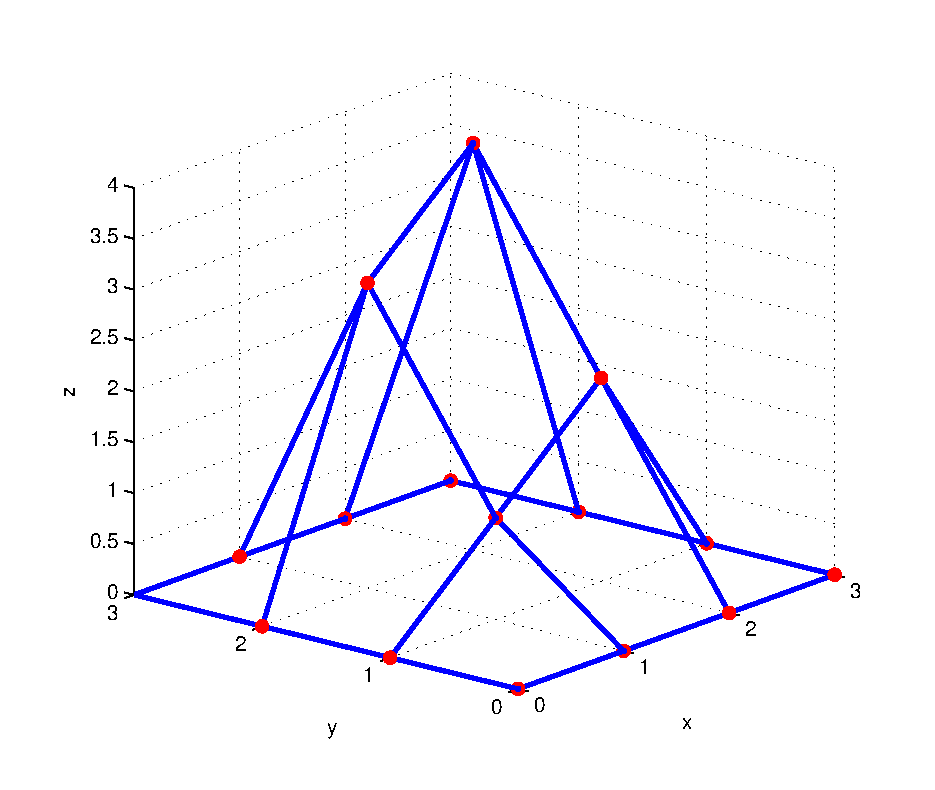
\includegraphics[width=11cm]{mesh1.eps}
\caption{Superficie elemental obtenida elevando los cuatros puntos centrales de la figura \ref{fig:mesh}.}
\label{fig:mesh1}
\end{figure}

La estructura de las matrices $X_m$ e $Y_m$ de los ejemplo anteriores, es la típica de las matrices de adyacencia de una retícula cuadrada; la matriz  $X_m$ tiene la filas repetidas y la matriz $Y_m$ tiene repetidas la columnas. En el ejemplo las matrices son cuadradas y definen una retícula de $4\times 4$ nodos. En general, podemos definir una retícula rectangular de $m\times n$ nodos. En este caso las matrices empleadas para definir la retícula tendrían dimensión $m\times n$.

Para dibujar en Matlab superficies podemos en primer lugar definir la retícula a partir de dos vectores de coordenadas empleando el comando \texttt{meshgrid}. En el ejemplo que acabamos de ver, hemos empleado una retícula que cubre el intervalo, $x\in[0,3]$ e $y\in[0,3]$. para definirlo creamos los vectores,

\begin{verbatim}
>> x=0:3
x =

     0     1     2     3

>> y=0:3
y =

     0     1     2     3
\end{verbatim}

A continuación empleamos el comando \texttt{meshgrid} para construir las dos matrices de adyacencia. Matlab se encargará de repetir las filas y columnas necesarias,

\begin{verbatim}
>> [Xm,Ym]=meshgrid(x,y)
Xm =

     0     1     2     3
     0     1     2     3
     0     1     2     3
     0     1     2     3


Ym =

     0     0     0     0
     1     1     1     1
     2     2     2     2
     3     3     3     3

\end{verbatim}

Una vez construidas las matrices de adyacencia, solo necesitamos una matriz de valores para $Z_m$. Si definimos por ejemplo,
\begin{verbatim}
>> Zm=zeros(size(Xm))

Zm =

     0     0     0     0
     0     0     0     0
     0     0     0     0
     0     0     0     0
\end{verbatim}

Podríamos representar la retícula plana de la figura \ref{fig:mesh}, empleando por ejemplo el comando \texttt{mesh(Xm, Ym, Zm)}.

\paragraph{mesh y surf.} Una vez que hemos visto como construir una retícula rectangular sobre la que construir una superficie, veamos como dibujarla con un ejemplo. Supongamos que queremos dibujar la superficie,
\begin{equation*}
z=x^3+y^2
\end{equation*}

En la región del plano, $x\in[-1.5,1.5]$, $y\in[-2,2]$. 

Igual que en el ejemplo inicial, lo primero que debemos hacer es construirnos una matrices de adyacencia que definan una retícula en la región de interés,
\begin{verbatim}
>> x=linspace(-1.5,1.5,25);
>> y=linspace(-2,2,50);
>> [Xm,Ym]=meshgrid(x,y);
\end{verbatim}

Es interesante notar que la región de interés no es cuadrada y que las matrices de adyacencia tampoco los son ($50\times 25$). Además los puntos no están espaciados igual en los dos ejes.

A continuación obtenemos la matriz de coordenadas z, aplicando la función a los puntos de la retícula,

\begin{verbatim}
>> Zm=Xm.^3+Ym.^2;
\end{verbatim}

\begin{figure}[h]
\centering
\subfigure[Función $z=x^3+y^2$ representada con \texttt{mesh}\label{fig:msh}]{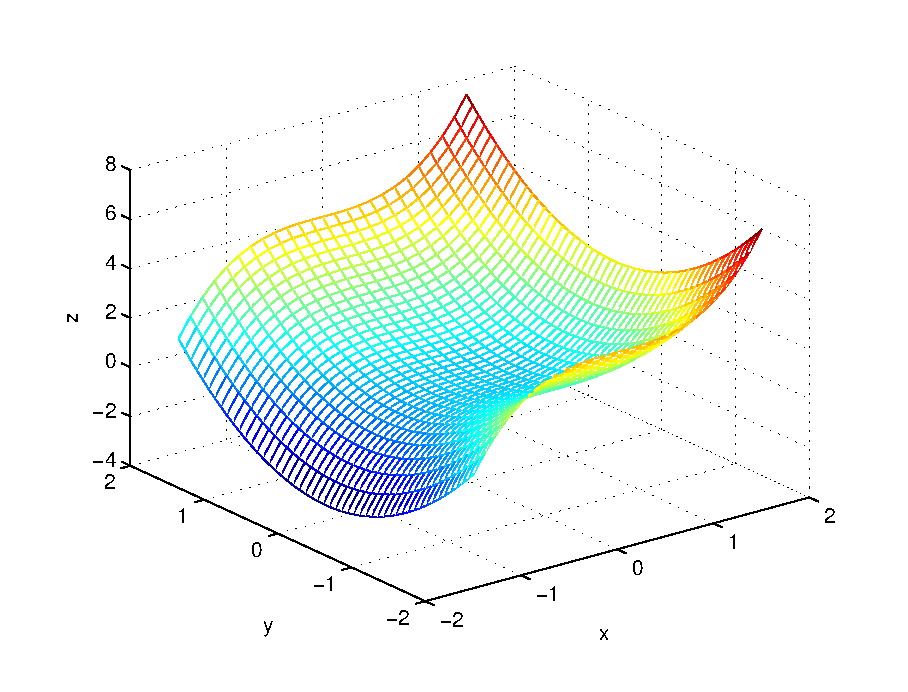
\includegraphics[width=8.5cm]{pa23.eps}} \qquad 
\subfigure[Función $z=x^3+y^2$ representada con \texttt{surf} \label{fig:sur}]{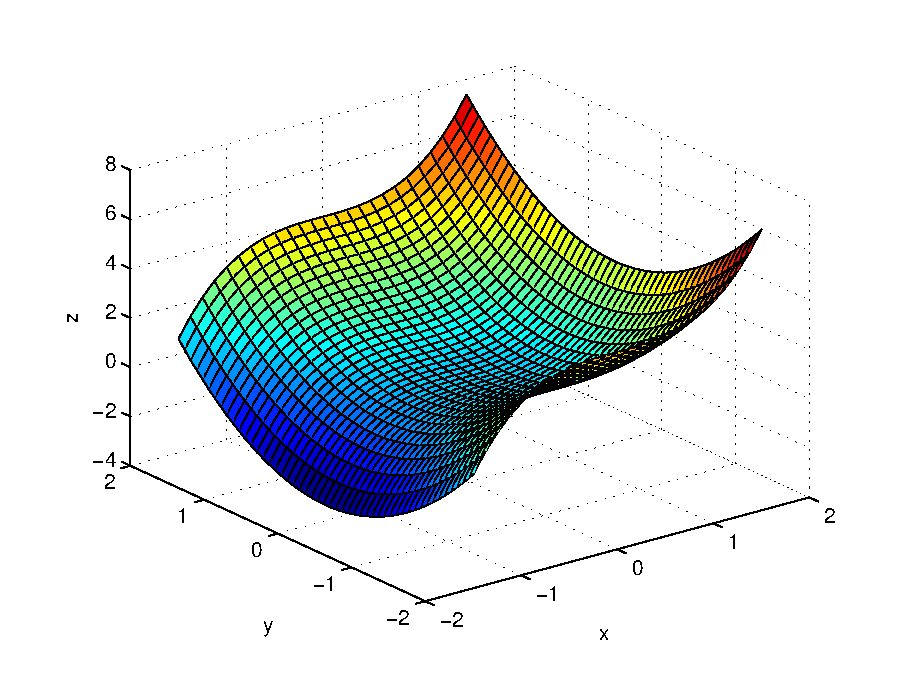
\includegraphics[width=8.5cm]{surf.eps}}\\
\caption{Comparación entre \texttt{mesh} y \texttt{surf}}
\end{figure}

Para representar la superficie podemos emplear el comando \texttt{mesh}. 
\begin{verbatim}
>> mesh(Xm,Ym,Zm)
\end{verbatim}

Este comando admite como variables de entrada las dos matrices de adyacencia empleadas para definir la retícula y la matriz $Z_m$ que contiene los valores calculados para la  variable z, en todos los puntos de la retícula. \texttt{mesh} traza la superficie en forma reticular, es decir, nos dibuja una malla en el espacio. El color de la malla depende del valor que toma la coordenada z. Podemos también representar la superficie haciendo uso del comando \texttt{surf}, empleando las mismas variables de entrada que en el caso de \texttt{mesh}. 
\begin{verbatim}
>> surf(Xm,Ym,Zm)
\end{verbatim}

La diferencia está en que ahora la superficie muestra las caras definidas por la malla de colores, según el valor que toma la variable $z$. la figura \ref{fig:msh} muestra el resultado de nuestro ejemplo empleando \texttt{mesh} y la figura \ref{fig:sur} muestra el resultado empleando \texttt{surf}.



Para figuras que presentan simetría radial, puede ser más conveniente, definir las retículas en coordenadas polares. así por ejemplo,

\begin{verbatim}
>> r=0:2/20:2;
>> theta=0:2*pi/36:2*pi;
>> [rm,them]=meshgrid(r,theta);
\end{verbatim}

Hemos cosntruido una retícula en las variables $r$ y $\theta$, si ahora definimos las matrices de adyacencia como las proyecciones sobre los ejes $x$ e $y$,

\begin{verbatim}
>> xm=rm.*cos(them);
>> ym=rm.*sin(them); 
\end{verbatim}

Obtenemos una retícula con simetría radial, centrada en el origen de coordenadas. Como la que se muestra en la figura, \ref{fig:retcir}.

\begin{figure}[h]
\centering
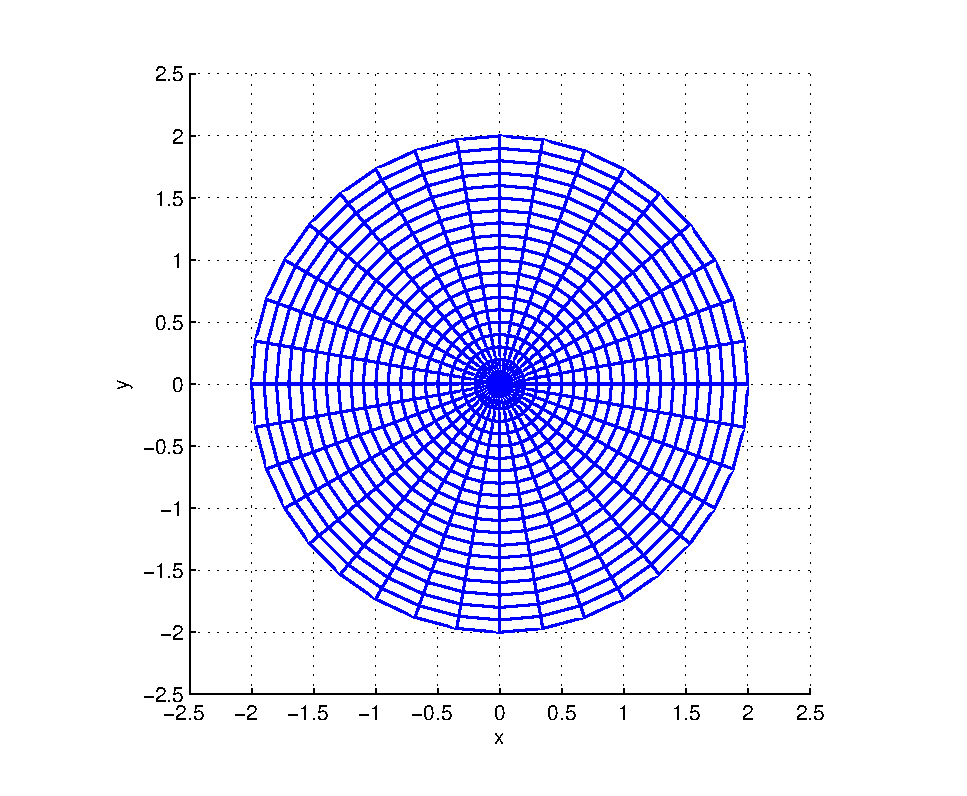
\includegraphics[width=12cm]{retcirc.eps}
\caption{retícula con simetría circular}
\label{fig:retcir}
\end{figure}

La retícula resulta muy adecuada para dibujar por ejemplo un cono (figura \ref{fig:cono}),

\begin{verbatim}
>> zm=2-sqrt(xm.^2+ym.^2);
>> mesh(xm,ym,zm)
\end{verbatim}

\begin{figure}[h]
\centering
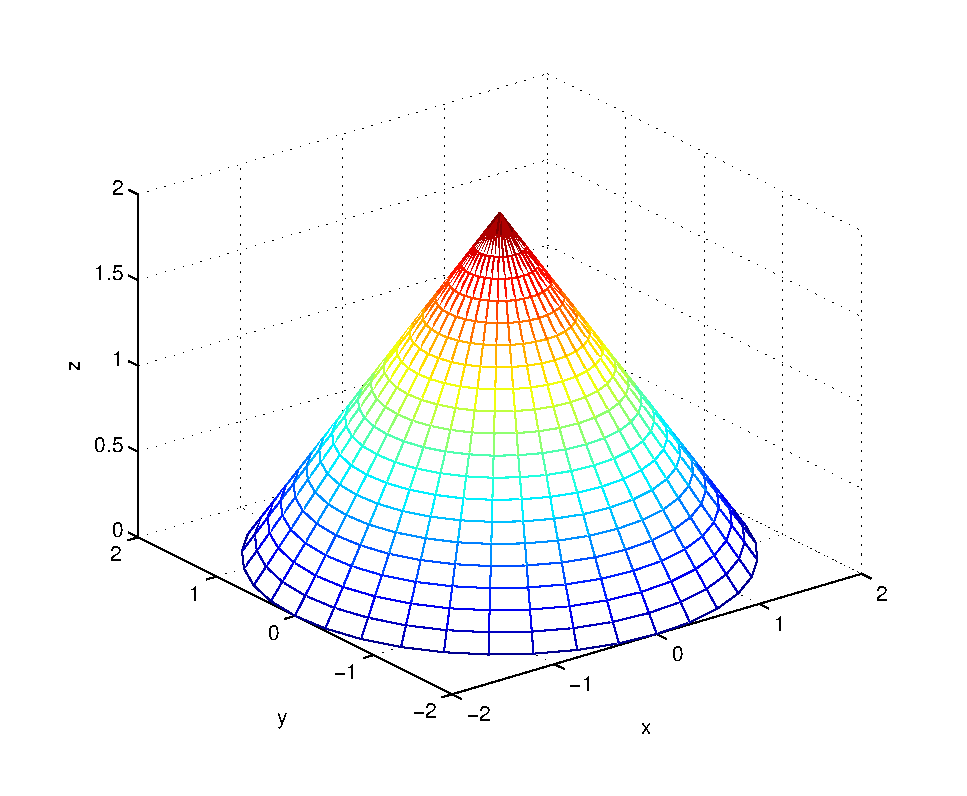
\includegraphics[width=12cm]{cono.eps}
\caption{Cono representado sobre una retícula circular}
\label{fig:cono}
\end{figure}

A continuación, se incluye el código de un script con varios ejemplos más de diseño de retículas circulares y gráficos de superficies en 3D. Los resultados se muestran en la figura \ref{fig:varios}

\begin{verbatim}
%este script (varios_g3d.m) incluye el diseño de varias retículas
%circulares para trazar gráficos de superficies en el espacio.

%retícula circular para un cono
 r=0:2/20:2;
 theta=0:2*pi/36:2*pi;
 [rm,them]=meshgrid(r,theta);
 
%calculamos las compontes en x e y partir de rm y thm,
 xm=rm.*cos(them);
 ym=rm.*sin(them);
 
%Definimos la componente z, a partir de la ecuación de un cono,
 zm=2-sqrt(xm.^2+ym.^2);

%lo dibujamos empleando el comando mesh
 mesh(xm,ym,zm)
 
%Para dibujar una esfera, podríamos emplear la misma retícula, pero sale
%más proporcionada, si de emplear intevalos de r equispaciodos, los hacemos
%proporcionales al águlo de elevacion (0,pi/2). Asique recalculamos r.

 r=2*cos(0:pi/2/18:pi/2); %tomamos 16 intervalos entre r=0 y r=2
%para theta usamos el mismo de antes, no hace falta volver a calcularlo.

%calculamos los puntos de la retícula en polares,
[rm,them]=meshgrid(r,theta);

%calculamos las componentes x e y a partir de rm y thm
 xm=rm.*cos(them);
 ym=rm.*sin(them);
 
 
 
 %definimos la componente z, como es la ecuación de una esfera, debemos
 %calcularla en dos partes,
 
 zm_mas=sqrt(4-(xm.^2+ym.^2));
 zm_menos=-sqrt(4-(xm.^2+ym.^2));
 
 %vamos a emplear la misma ventana gráfica en la que hemos dibujado el
 %cono, asi que pedimos a Matlab que retenga lo ya dibujado,
 
 hold on
 
 %para que no salga un dibujo encima del otro, dibujamos la esfera
 %desplazando su origen al punto (3,3,0)
 %emplearemos ahora el comando surf para representarla
 
 %primero representamos la mitad superior
  surf(xm+3,ym+3,zm_mas)
 
 %y despues la parte inferior
  surf(xm+3,ym+3,zm_menos)
  
 %por último vamos a obtener la gráfica de un cilidro vertical, Para ello,
 %volvemos a alterar los valore de r. Costruimos un vector que repita
 %siempre los mismos valores y le damos tanto elementos como divisiones
 %'verticales queramos que tenga el cilindro, por ejemplo 20
 r=2*ones(1,20); 
 
 %volvemos a crear la reticula
 [rm,them]=meshgrid(r,theta);

%calculamos las componentes x e y a partir de rm y thm
 xm=rm.*cos(them);
 ym=rm.*sin(them);
 
 % Para calcular los valores de z, debemos dividir la altura total que
 % queremos dar al cilindro entre el número de divisiones en r que tiene la
 % retícula original por ejemplo si la altura fuera 2
  z=2/(length(r)-1)*(0:length(r)-1);
 % Tenemos una columna de la matriz z, pero necesitamos repetirlas para
 % cada valor de them,
  zm=ones(size(xm))*diag(z);
 
 %podemos ahora dibujar en cilindro. Como hemos hecho con la esfera, lo
 %vamos a desplazar a una posición en la que no se sobreponga a otra
 %figura, por ejemplo al punto (+3 -3 -1).
 
 %lo vamos a representar usando de nuevo en comando mesh
 
 mesh(xm+3,ym-3,zm-1)

\end{verbatim}

\begin{figure}[h]
\centering
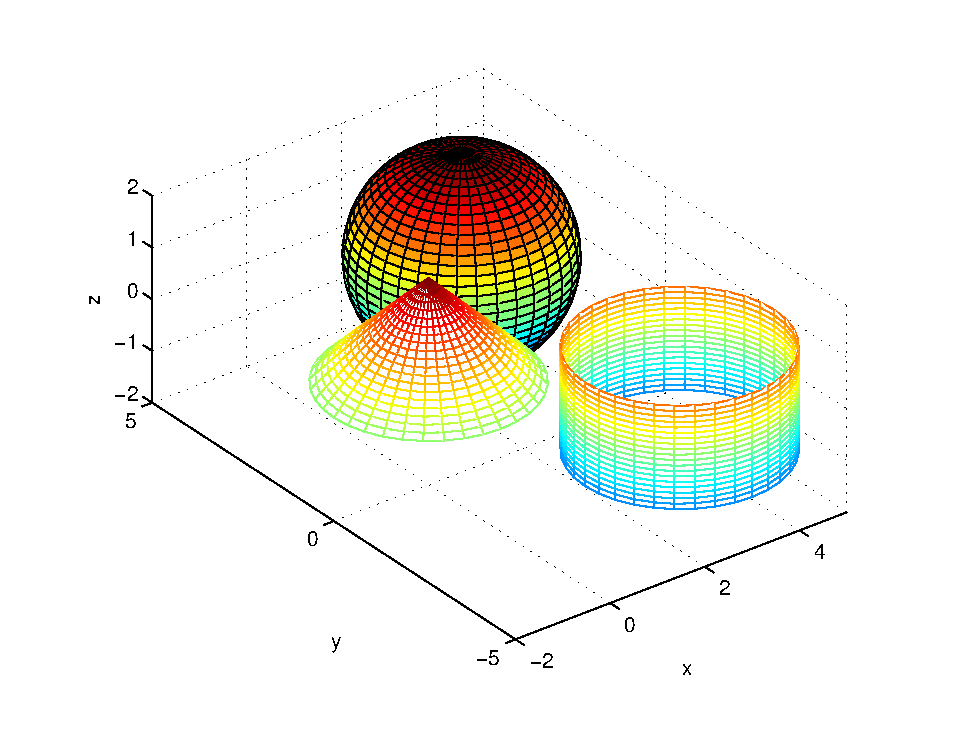
\includegraphics[width=12cm]{varios.eps}
\caption{retícula con simetría circular}
\label{fig:varios}
\end{figure}

\paragraph{contour, contour3, meshc y surfc.} Este comandos permiten obtener y dibujar las curvas de nivel de una superficie. Su uso es idéntico al de los comandos anteriores. Es decir, también necesitan que se defina una retícula en el plano $(x,y)$, y se calculen los valores que tomará  la variable z sobre los puntos de la retícula.

\begin{figure}[h]
\centering
\subfigure[contour  \label{fig:contour}]{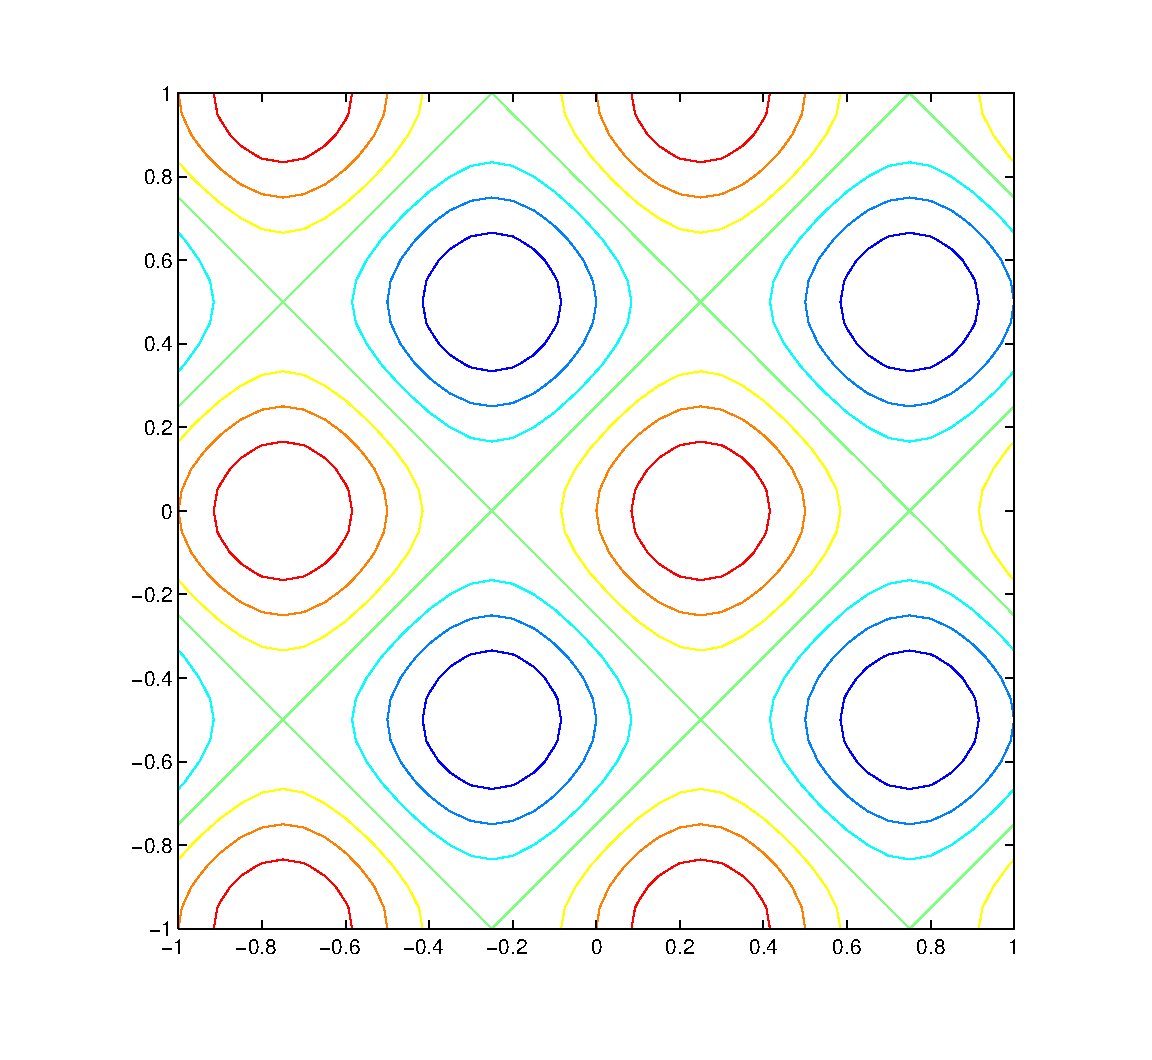
\includegraphics[width=6.5cm]{contour.eps}} \qquad 
\subfigure[contour3 \label{fig:contour3}]{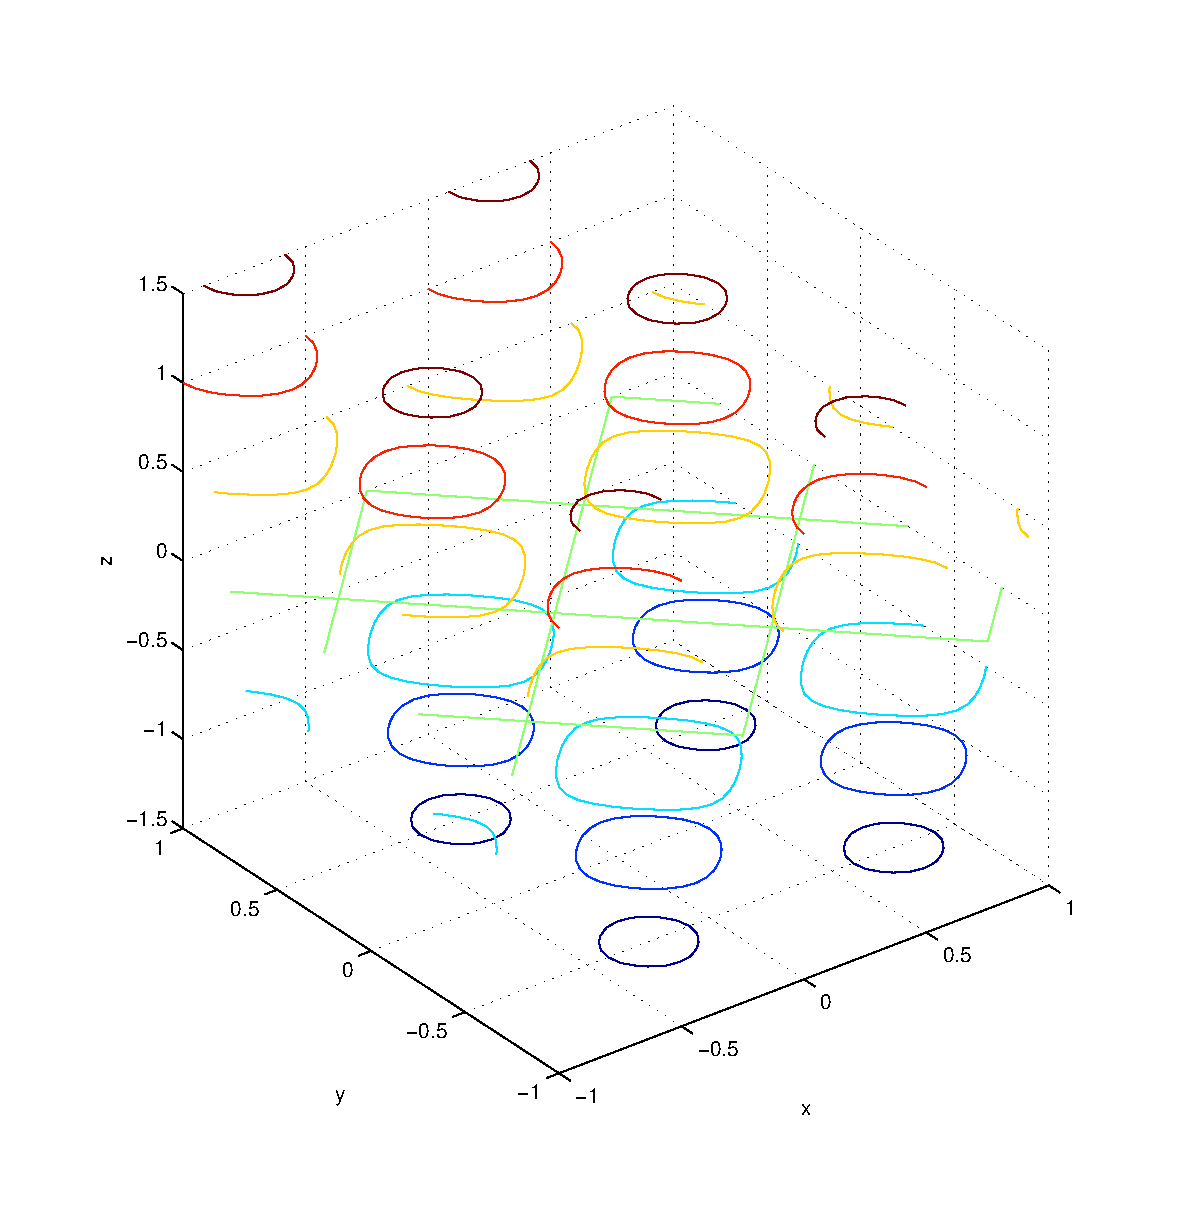
\includegraphics[width=6.5cm]{contour3.eps}}\\
\subfigure[meshc \label{fig:mesh3}]{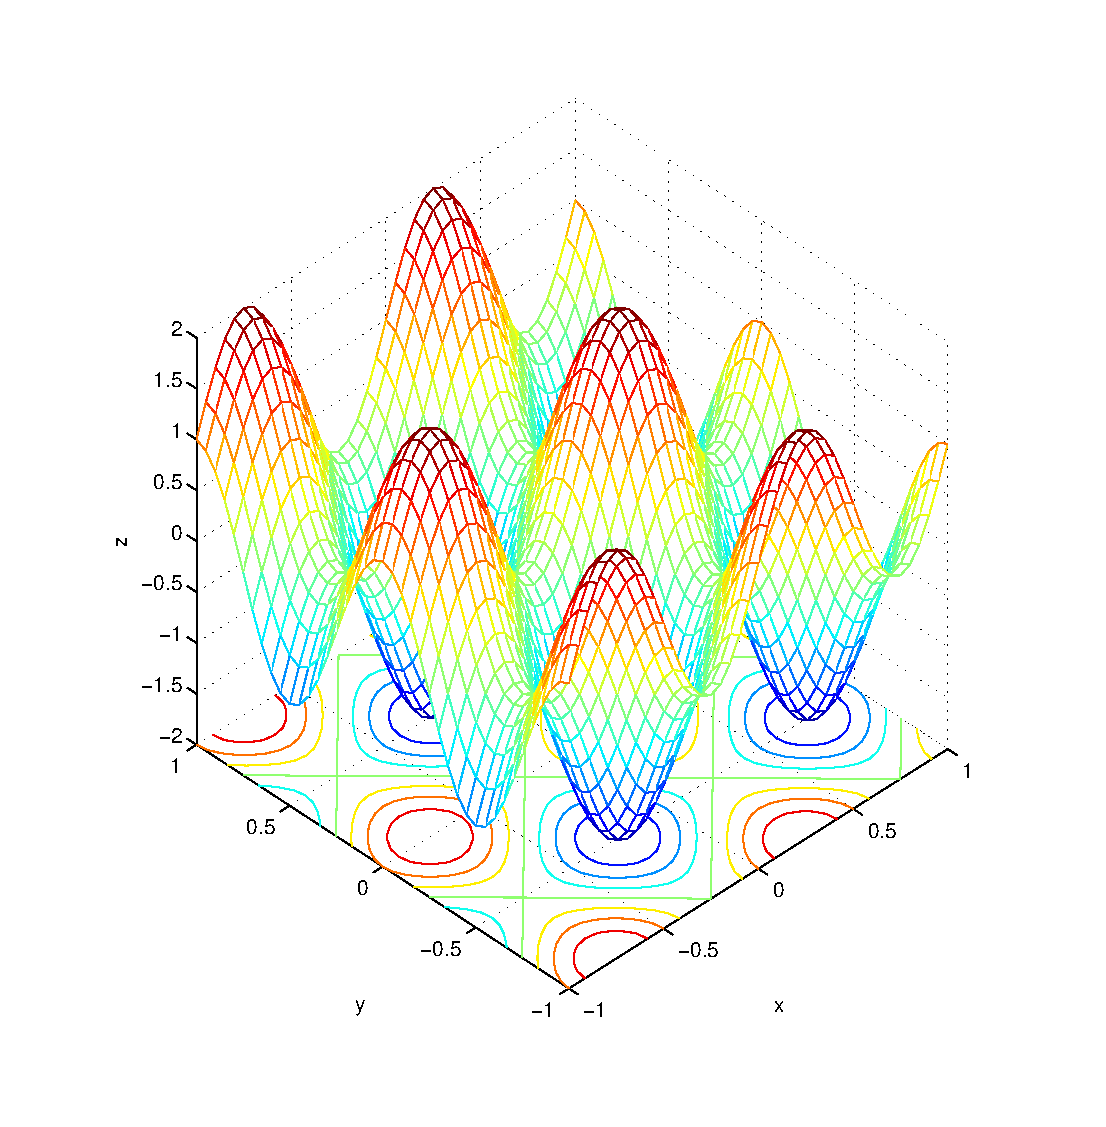
\includegraphics[width=6.5cm]{meshc.eps}}\qquad
\subfigure[surfc \label{fig:surf3}]{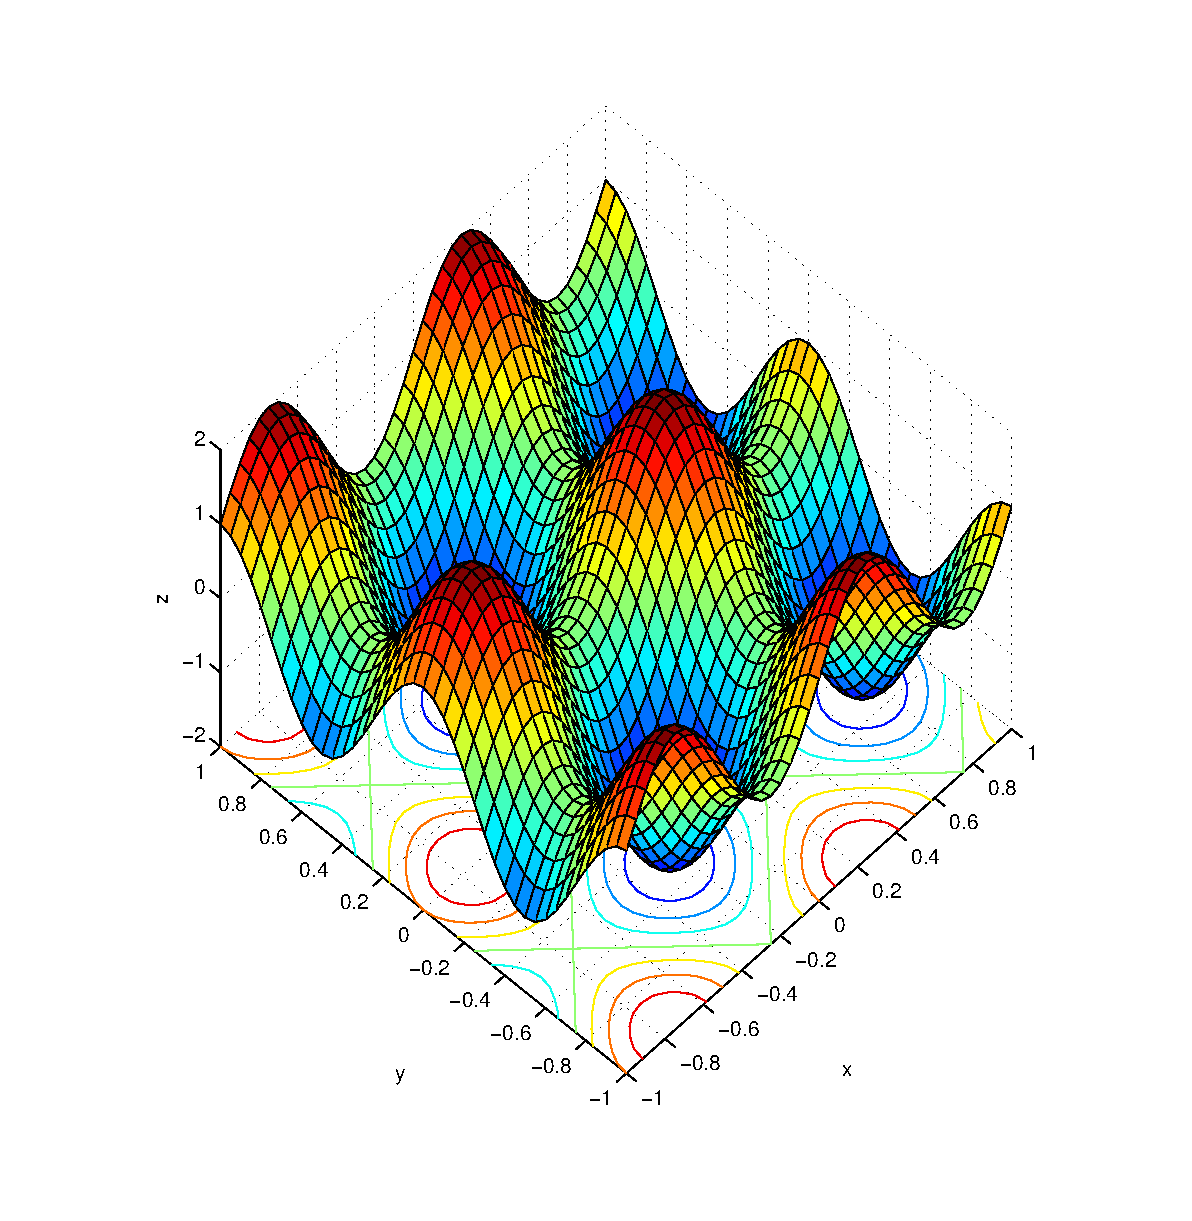
\includegraphics[width=6.5cm]{surfc.eps}}\\
\caption{Comparación entre los resultados de \texttt{contour}, \texttt{contour3}, \texttt{meshc} y \texttt{surfc}, para la obtención de las curvas de nivel de una superficie. }
\end{figure}

Veamos su funcionamiento con un último ejemplo. Obtenemos una retícula cuadrada, calculamos sobre ella los puntos de la superficie,

\begin{equation*}
z=\sin(2\pi x)+cos(2\pi y)
\end{equation*}

\begin{verbatim}
>> x=[-1:0.05:1];
>> y=x;
>> [xm,ym]=meshgrid(x,y);
>> zm=sin(2*pi*xm)+cos(2*pi*ym);
>> contour(xm,ym,zm)
>> contour3(xm,ym,zm)
>> meshc(xm,ym,zm)
>> surfc(xm,ym,zm)
\end{verbatim}



La figura \ref{fig:contour} muestra los resultados de aplicar el comando \texttt{contour}. La gráfica representa las curvas de nivel de la superficie dibujadas sobre el plano $(x,y)$. El comando \texttt{contour3} ( figura \ref{fig:contour3}) representa de nuevo las curvas de nivel, pero sitúa cada una a su correspondiente altura $z$.  Por último \texttt{meshc} y \texttt{surfc} representan la superficie y añaden en el plano $(x,y)$ la representación de las curvas de nivel correspondiente a la superficie.

Para terminar la sección dedicada a los gráficos, vamos a combinar el comando \texttt{mesh} con el comando \texttt{plot3} para dibujar una curva sobre una superficie. Tomaremos como ejemplo la superficie,
\begin{equation*}
z=\frac{sin\left((\pi x)^2+(\pi y^2)\right)}{(\pi x)^2+(\pi y^2)}
\end{equation*}

Sobre la que trazamos la curva,

\begin{equation*}
y=sin(\pi x),\\
\end{equation*}

\begin{figure}[h]
\centering
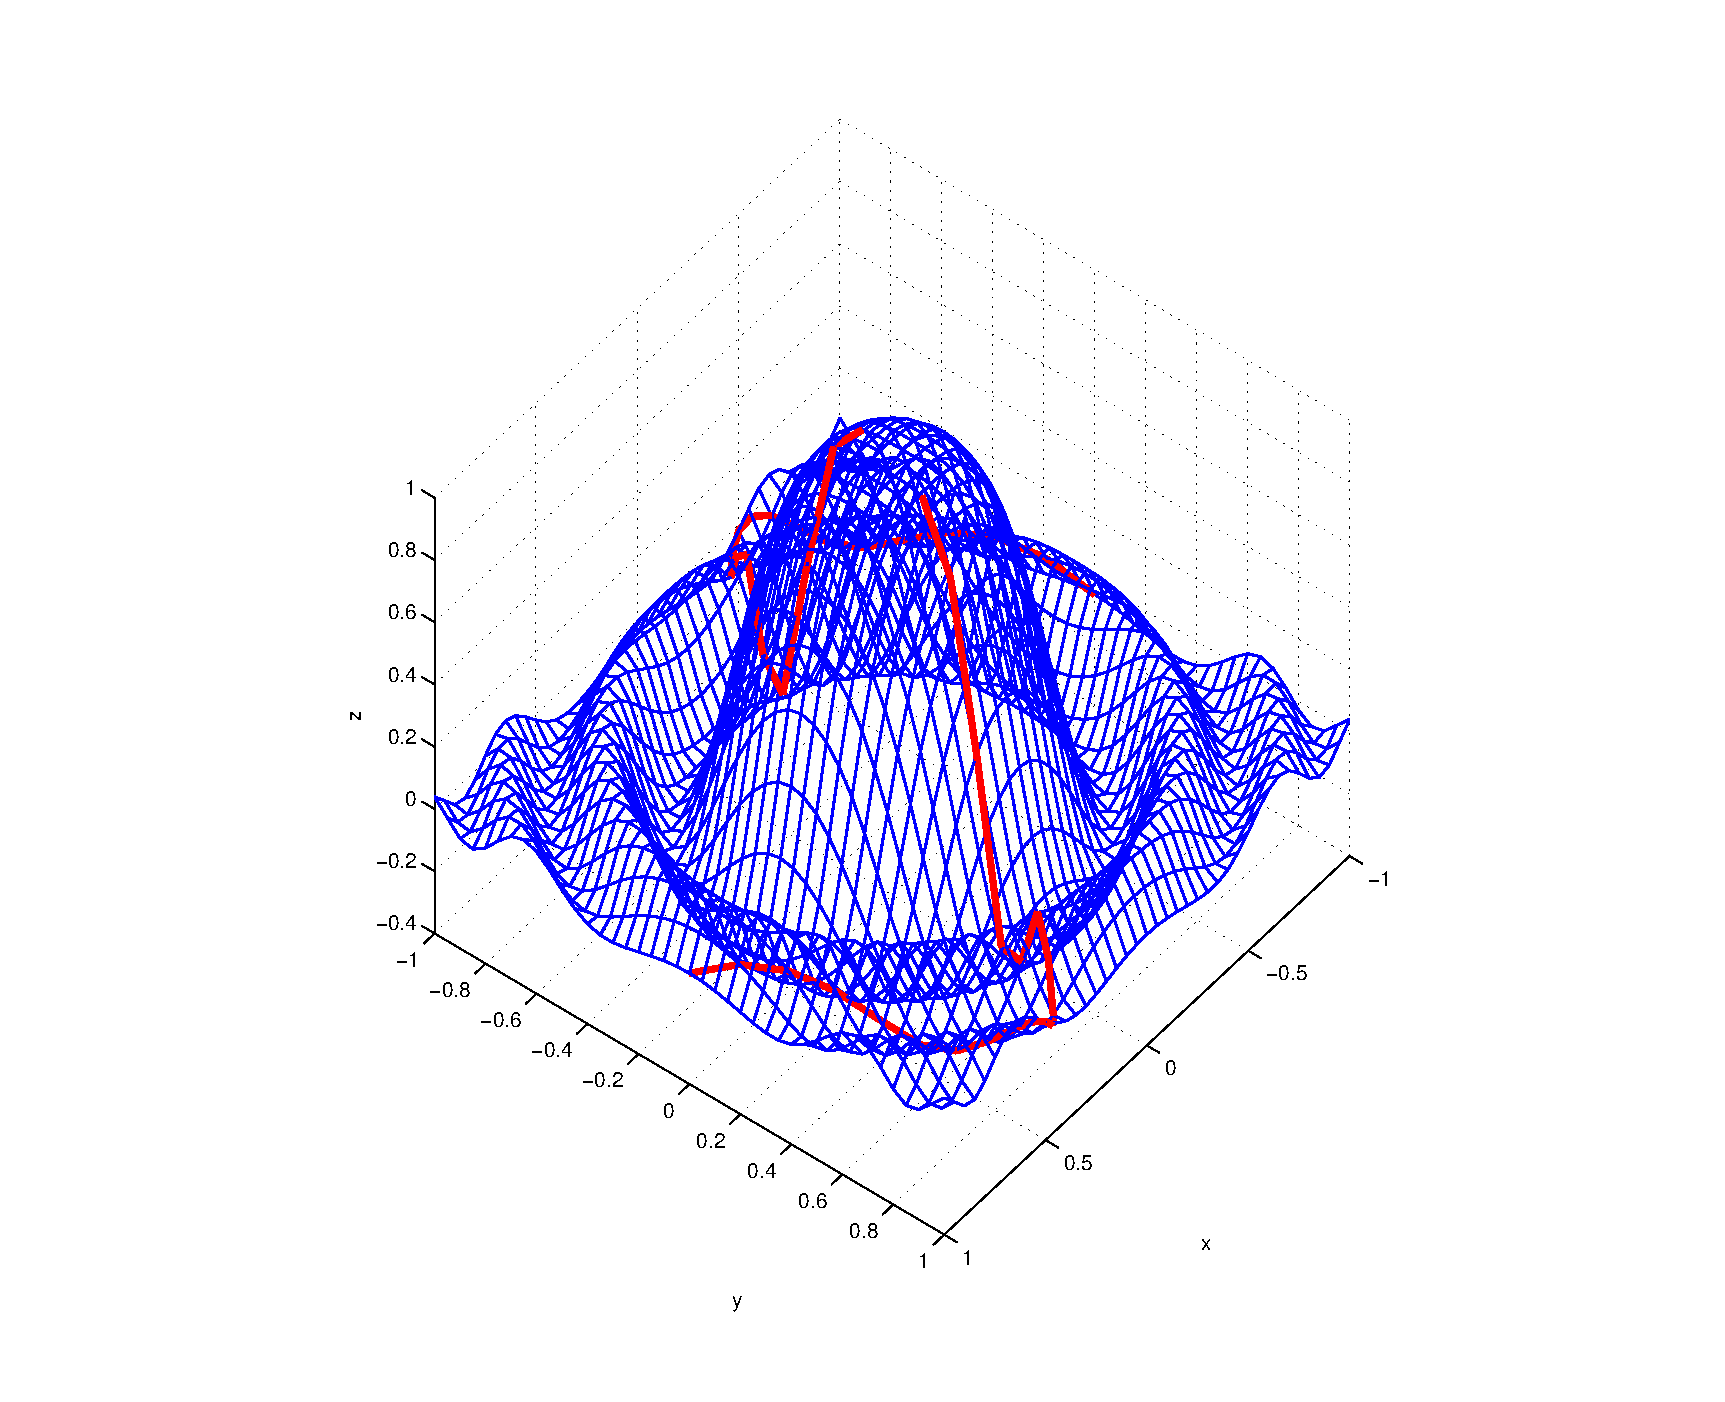
\includegraphics[width=11cm]{linsu.eps}
\caption{Curva trazada sobre una superficie}
\label{fig:cvsurf}
\end{figure}

Es decir, obtenemos el valor de los puntos $z$ de la superficie para los pares de puntos $[x, y = sin(\pi x)]$, que definen la curva trazada sobre la superficie $z$,

\begin{verbatim}
>> x=[-1:0.05:1];
>> y=x;
>> [xm,ym]=meshgrid(x,y);
>> zm=sin((pi*xm).^2+(pi*ym).^2)./((pi*xm).^2+(pi*ym).^2);
>> mesh(xm,ym,zm)
>> y=sin(pi*x);
>> z=sin((pi*x).^2+(pi*y).^2)./((pi*x).^2+(pi*y).^2);
>> hold on
>> plot3(x,y,z)
\end{verbatim}

Es importante insistir en que a lo largo de esta sección nos hemos limitado a introducir algunas de las posibilidades gráficas de Matlab. Para obtener una visión completa de las mismas es imprescindible leer con detenimiento la ayuda de Matlab.
%\chapter{Introducción a Numpy\\ Introduction to Numpy}\index{Numpy} \index[eng]{Numpy}
\chaptermark{Intro. a Numpy \textreferencemark\ Intro to Numpy}
\epigraph{When the going gets tough, the tough get going}{Popular Witticism (US)}
\begin{paracol}{2}
\section{Numpy: un paquete de Python para cálculo nu\-mérico}
En el capítulo \ref{ch:intpr}, vimos cómo importar mó\-dulos de python en un script o directamente en el terminal de Ipython, de modo que podamos reutilizar el código contenido en ellos. Numpy es un libraría de python que contiene funciones y variables específicamente diseñadas para el cálculo numérico. Está estructurada en forma de módulos y submódulos de modo que para utilizarla en nuestros programas basta  importarla en nuestros script, importar sus submodulos o importar sus funciones.
La base de Numpy la constituyen objetos y operaciones algebráicas. En esta sección vamos a repasar algunos conceptos fundamentales de  álgebra lineal y cómo pueden manejarse empleando Python. No daremos definiciones precisas ni tampoco demostraciones, ya que tanto unas como otras se verán en detalle en la asignatura de álgebra.

\paragraph{Matrices.} Desde un punto de vista funcional definiremos una matriz como una tabla bidimensional de números ordenados en filas y columnas,
\switchcolumn

\section{Numpy: a Python library for scientific computing}
In chapter \ref{ch:intpr}, we have seen how to import Python modules to a script or to the Ipython console. In this way, we can reuse the code available in the modules. Numpy is a Python library with functions and variables specifically intended to perform scientific computing. Numpy is structured in modules and submodules so that we can import the whole library, its submodules, or just any of its functions into our scripts. The background of Numpy is built of algebraic objects and operations. In this section, we will review some fundamental notions of linear algebra and how to deal with them using Numpy. We will not provide formal definitions or demonstrations because both will be studied in detail in algebra during the next term.
\paragraph{Matrices} From a functional perspective, we will define a matrix as a table of numbers ordered by rows and columns,
\end{paracol}

\begin{equation*}
A=
\begin{pmatrix}
1& \sqrt{2}& 3.5& 0\\
-2& \pi& -4.6& 4\\
7& -19& 2.8& 0.6
\end{pmatrix}
\end{equation*}

\begin{paracol}{2}
Cada línea horizontal de números constituye una \emph{fila} de la matriz y cada línea vertical una \emph{columna} de la misma.

A una matriz con $m$ filas y $n$ columnas se la denomina matriz de orden $m\times n$. $m$ y $n$ son la dimensiones de la matriz y se dan siempre en el mismo orden: primero el número de filas y después el de columnas. Así, la matriz $A$ del ejemplo anterior es una matriz $3\times 4$, y como esta formada por números reales se dice que $A\in\mathbb{R}^{3\times 4}$. El orden de una matriz expresa el tamaño de la matriz.

Dos matrices son iguales si tienen el mismo orden, y los elementos que ocupan en ambas matrices los mismo lugares son iguales.

Una matriz es cuadrada, si tiene el mismo número de filas que de columnas. Es decir es de orden $n\times n$.

Mientras no se diga expresamente lo contrario, emplearemos letras mayúsculas $A, B, \cdots$ para representar matrices. La expresión $A_{m\times n}$ indica que la matriz $A$ tiene dimensiones $m \times n$. Para denotar los elementos de una matriz, emplearemos la misma letra en minúsculas empleada para nombrar la matriz, indicando mediante subíndices, y siempre por este orden, la fila y la columna a la que pertenece el elemento. Así por ejemplo $a_{ij}$ representa al elemento de la matriz $A$, que ocupa la fila $i$ y la columna $j$.
\switchcolumn
Each horizontal line of numbers forms a matrix row, and each vertical line a matrix column.
A matrix with $m$ rows and $n$ columns is denoted as a matrix of order $m\times n$. $m$ and $n$ are the matrix dimensions, and they are always defined in the same order: first, the number of rows and then the number of columns. So matrix $A$ in the example above is a $3\times 4$ matrix, and as it is built of real numbers, we say that $A\in \mathbb{R}^{3\times 4}$. The matrix order defines the size of the matrix.

Two matrices are equal if they have the same order and the elements located in both matrices in the same place are equal. A matrix is square when it has the same number of rows and columns. That is, it is an $n\times n$ matrix.

From now on, we will use capital letters $A,\ B,\cdots$ to name matrices. The expression $A_{m\times n}$ means that matrix $A$ has dimensions $m\times n$. We will refer to the elements of a matrix using the same letter used to name the matrix but in lowercase and using subindexes to indicate the row and column the element belongs to. The first subindex always represents the row, and the second is the column. For instance, $a_{ij}$ Represents the matrix $A$ element that belongs to row $i$ and to column $j$.
\end{paracol}
\begin{equation*}
A=
\begin{pmatrix}
1& \sqrt{2}& 3.5& 0\\
-2& \pi& -4.6& 4\\
7& -19& 2.8& 0.6
\end{pmatrix}
\rightarrow a_{23}=-4.6
\end{equation*}
\begin{paracol}{2}
\paragraph{vectores}
A una matriz compuesta por una sola fila, la denominaremos vector fila. A una matriz compuesta por una sola columna la denominaremos vector columna. Siempre que hablemos de un vector, sin especificar más, entenderemos que se trata de un vector columna.\footnote{Esta identificación de los vectores como vectores columna no es general. La introducimos porque simplifica las explicaciones posteriores.} Para representar vectores, emplearemos letras minúsculas. Para representar sus elementos añadiremos a la letra que representa al vector un subíndice indicando la fila a la que pertenece el elemento.
\switchcolumn
We call a matrix formed by a single row a row vector. We call a matrix formed by a single column a column vector. Whenever we speak of a vector without further specification, we consider it a column vector.\footnote{This identification of a vector with a column vector is by no means general. We introduce it because it simplifies the exposition.}. To name vectors, we will use lowercase letters. To name the elements of a vector, we will add a subindex to the letter representing the vector to show the row the element belongs to. 
\end{paracol}
\begin{equation*}
a=
\begin{pmatrix}
a_1\\
a_2\\
\vdots \\
a_i\\
\vdots \\
a_n
\end{pmatrix}
\end{equation*}
\begin{paracol}{2}
Podemos asociar los puntos del plano con los vectores de dimensión dos. Para ello, usamos una representación cartesiana, en la que los elementos del vector son los valores de las coordenadas $(x,y)$ del punto del plano que representan. Cada vector se representa gráficamente mediante una flecha que parte del origen de coordenadas y termina en el punto $(x,y)$ representado por el vector. La figura \ref{fig:vectores} representa los vectores,
\switchcolumn
We can establish a relationship between the plane points and two-dimensional vectors. To do so, we use a Cartesian representation, in which the elements of a vector are the $(x,y)$ coordinates of the point of the plane they represent. Each vector is drawn using an arrow that starts at the origin of the coordinates and ends at the point $(x,y)$ represented by the vector. Figure \ref{fig:vectores} represents vectors, 
\end{paracol}
\begin{equation*}
a=
\begin{pmatrix}
1\\
2
\end{pmatrix},
b=
\begin{pmatrix}
2\\
-3
\end{pmatrix},
c=
\begin{pmatrix}
0\\
-2
\end{pmatrix}
\end{equation*}


\begin{figure}[h]
\centering
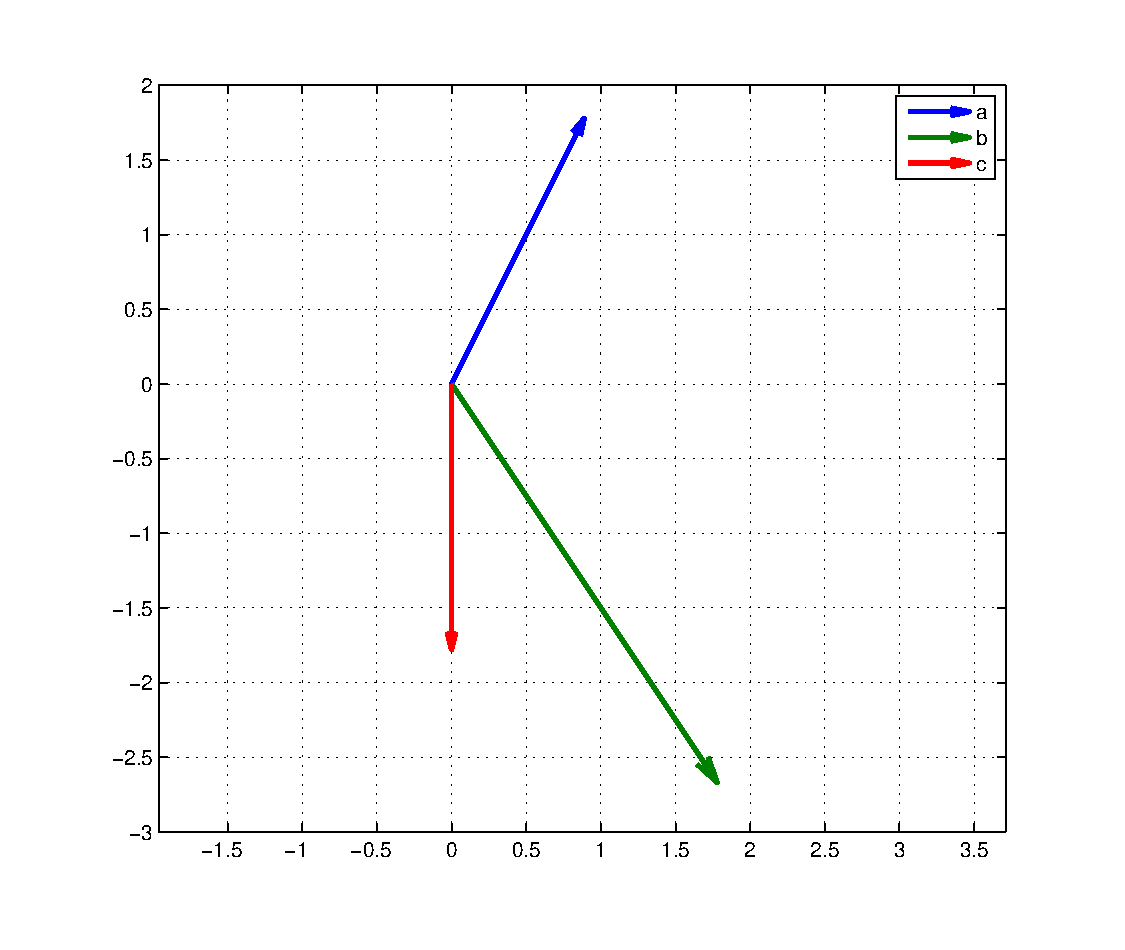
\includegraphics[width=7cm]{vectores.eps}
\bicaption{Representación gráfica de vectores en el plano}{Graphic of vectors on the plane}
\label{fig:vectores}
\end{figure}

\begin{paracol}{2}
De modo análogo, podemos asociar vectores de dimensión tres con puntos en el espacio tridimensional. En este caso, los valores de los elementos del vector corresponden con la coordenadas $(x,y,z)$ de los puntos en el espacio. La figura \ref{fig:vectores3} muestra la representación gráfica en espacio tridimensional de los vectores,
\switchcolumn
Likewise, we can associate vectors of dimension three with points in the 3D space. In this case, the vector elements represent the coordinates $(x,y,z)$ of the points in the space. Figure \ref{fig:vectores3} shows a graphic representation of vectors,
\end{paracol}
\begin{equation*}
a=
\begin{pmatrix}
1\\
2\\
1
\end{pmatrix},
b=
\begin{pmatrix}
2\\
-3\\
-1
\end{pmatrix},
c=
\begin{pmatrix}
0\\
-2\\
1
\end{pmatrix}
\end{equation*}

\begin{figure}[h]
\centering
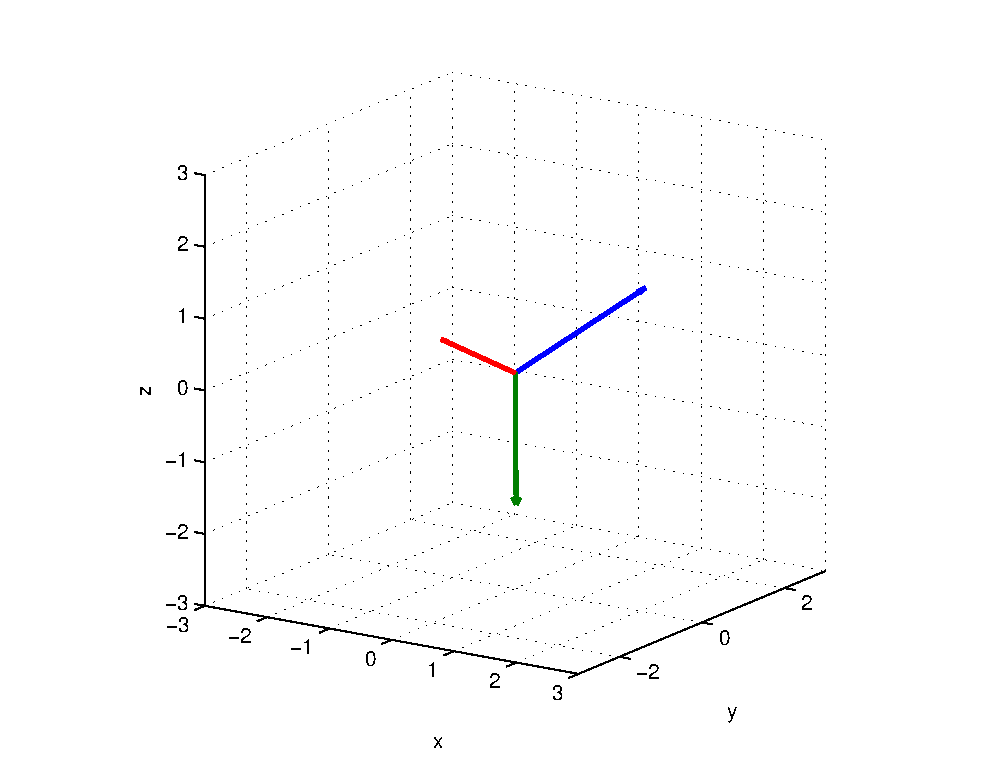
\includegraphics[width=9cm]{vectores3.eps}
\bicaption{Representación gráfica de vectores en el espacio 3D}{Graphic of vector in the 3D space}
\label{fig:vectores3}
\end{figure}
\begin{paracol}{2}
Evidentemente para vectores de mayor dimensión, no es posible obtener una representación gráfica. Si embargo muchas de las propiedades geométricas, observables en los vectores bi y tridimensionales, pueden extrapolarse a vectores de cualquier dimensión.

\subsection{Vectores y matrices en\\ Numpy.} \index{Vectores!en Numpy} \index{Matrices!en Numpy} 
\paragraph{Matrices.} Una de las característica más interesantes de Numpy, es la posibilidad de crear fácilmente matrices. Se pueden crear de diferentes maneras, la más elemental de todas ellas, emplea la funcion de Numpy \mintinline{python}{array} aplicada a una lista de filas de la matriz que se quiere construir. Cada fila debe ser a su vez una lista de números. Evidentemente, para que se pueda construir la matriz, todas las filas deben tener el mismo número de elementos. El siguiente ejemplo muestra como construir una matriz de dos filas y tres columnas,

\switchcolumn 
Obviously, it is impossible to get a graphic representation for vectors of larger dimensions. Nevertheless, many geometrical properties owned by 2D and 3D vectors can be applied to vectors of whatever dimension.

\subsection{Vetors and matrices in Numpy.}\index[eng]{Vectors! in Numpy}\index[eng]{Matrices! in Numpy}
\paragraph{Matrices.} One interesting feature of numpy is that it allows us to create matrices easily. There are several methods to create them, but using the Numpy function \mintinline{python}{array} with a Python list with the rows of the matrix we want to build is probably the easiest method. Each row should be, in turn, a list of numbers, i.e., matrix elements. Of course, to build a matrix all rows should have the same number of elements. The following example shows how to build a matrix of two rows and three columns.
\end{paracol}

\begin{center}
    \begin{minipage}{0.4\textwidth}
    \begin{minted}{python}
In [3]: import numpy as np

In [4]: A = np.array([[1,2,3],[4,5,6]])

In [5]: print(A)
[[1 2 3]
 [4 5 6]]

In [6]: L = [[1,2,3],[4,5,6]]

In [7]: B = np.array(L)

In [9]: print(L)
[[1, 2, 3], [4, 5, 6]]

In [10]: print(B)
[[1 2 3]
 [4 5 6]]
 \end{minted}
\end{minipage}
 \end{center}
\begin{paracol}{2} 
Lo primero que hacemos es importar Numpy, lo importamos usando como alias la abreviatura np, porque es más cómodo a la hora de llamar a funciones específicas de Numpy.  Hemmos construido dos matrices iguales \mintinline{python}{A} y \mintinline{python}{B}. En el primer caso hemos creado directamente dentro de la llamada a la función \mintinline{python}{array}, la lista a partir de la cual construimos la matriz. En el segundo caso, hemos construido primero una lista \mintinline{python}{L}, y luego hemos empleado dicha lista como variable de entrada de la función \mintinline{python}{array}. Si nos fijamos en las líneas [9] y [10], vemos como Python distingue la lista ---todos sus elementos aparacen representados en la misma línea---, de la matriz en la que cada fila ocupa una línea distinta. Podemos construir matrices a partir de listas y variables ya definidas, siempre que seamos coherentes con el criterio de que cada fila se cree a partir de una lista y que todas las filas tengan los mismos elementos,
\switchcolumn
First, we import Numpy; we do it using \mintinline{python}{np} as an alias. The reason is that \mintinline{python}{np} is shorter than \mintinline{python}{numpy}, and it eases the calls to specific Numpy functions. We have built two identical matrices \mintinline{python}{a} and \mintinline{python}{B}. In the first case, we have straightforwardly created the list needed to make the matrix inside the call to the function \mintinline{python}{array}. In the second case, we first created a list \mintinline{python}{L}, and then we used it as an input variable to the function \mintinline{python}{array}. Focusing on lines [9] and [10], we see how Python can tell a list and a matrix apart. For a list, Python represents all elements in the same line. For a matrix, each row is written in a different line.
We can build matrices from lists and variables already defined as long as we follow the criteria that each row be created from a list and all rows have the same number of elements,  
\end{paracol}
\begin{center}
    \begin{minipage}{0.4\textwidth}
        \begin{minted}{python}
In [23]: a =1; b= 2; c =3

In [24]: d =[4,5,6]

In [25]: C = np.array([[a,b,c],d])

In [26]: print(C)
[[1 2 3]
 [4 5 6]]

In [27]: C = np.array([[a,b,c],d,[7,8,9]])

In [28]: print(C)
[[1 2 3]
 [4 5 6]
 [7 8 9]]
        \end{minted}
    \end{minipage}
\end{center}
\begin{paracol}{2}
\paragraph*{Indexación.} \index{Numpy!indexación}Al igual que se hace en álgebra, Numpy es capaz de referirse a un elemento cualquiera de una matriz empleando índices para determinar su posición (fila y columna) dentro de la matriz.
\switchcolumn
\paragraph{Indexing}\index[eng]{Numpy!Indexing} As in algebra, in NUmpy is also possible to refer any element of a matrix using indexes to indicate its position (row and column) in the matrix. 
\end{paracol}
\begin{equation*}
A=
\begin{pmatrix}
a_{11}&a_{12}&a_{13}\\
a_{21}&a_{22}&a_{23}\\
a_{31}&a_{32}&a_{33}
\end{pmatrix}
\end{equation*}

\begin{paracol}{2}
Sin embargo,  el criterio para referirse a un elemento concreto de una matriz, en Numpy está heredado de las listas: se indica el nombre de la variable que contiene la matriz y a continuación, entre corchetes y separados por una coma, el índice de su fila y después él de su columna \textbf{pero empezando a contar desde $0$}. Es decir, la primera fila de una matriz de dimensión $m\times n$ es la fila $0$ y la última es la fila $m-1$. De modo análogo su primera columna es la $0$ y su última columna es la $n-1$,
\switchcolumn
However, the Numpy criteria to refer to a specific element inside a matrix has been borrowed from Python Lists: we write the name of the matrix followed by the row and column indexes of the element we are interested in, enclosed in a square bracket and separated by a comma. The point is that we \textbf{count the rows and columns starting at $0$}. Thus, the first row of a matrix with dimensions $m\times n$ is the row $0$, and the last is the row $m-1$. Likewise, its first column is column $0$, and the last one is column $n-1$, 
\end{paracol}
\begin{center}
    \begin{minipage}{0.3\textwidth}
        \begin{minted}{python}
In [31]: print(C)
[[1 2 3]
 [4 5 6]
 [7 8 9]]

In [32]: C[1,2]
Out[32]: 6

In [33]: C[0,0]
Out[33]: 1
        \end{minted}
    \end{minipage}
\end{center}

\begin{paracol}{2}
Numpy puede seleccionar dentro de una matriz no solo elementos aislados, sino también submatrices completas. 
Para ello, emplea un símbolo reservado, el símbolo \emph{dos puntos} $:$. Este símbolo se emplea para recorrer valores desde un valor inicial hasta un valor final, con un incremento o paso fijo. La sintaxis es: \mintinline{python}{inicio:fin:paso}. Es importante tener en cuenta que Numpy detendrá la cuenta en el valor \mintinline{python}{stop-step}. Además, si no indicamos el tamaño del paso, Numpy tomará por defecto un paso igual a uno. En este caso basta emplear \mintinline{python}{start:stop}
\switchcolumn
Inside a matrix, Numpy can select single elements and whole submatrices. To do so, it uses the colon : symbol as a special symbol. Using a fixed step, we use this symbol to cover a set of values from a start (initial) value to a stop (final) one. The syntax is simple: \mintinline{python}{start:stop:step}. Beware! Numpy will stop the count in the step \mintinline{python}{stop-step}. Besides, if we leave apart the step size, Numpy will take a step equal to one. In this case, the expression is just \mintinline{python}{start:stop}
\end{paracol}

\begin{center}
        \begin{minted}{python}
In [87]: D = numpy.array([[1.,2.,3.],[4.,5.,6.],[-2,-3,0],[3,2,1]])

In [88]: print(D)
[[ 1.  2.  3.]
 [ 4.  5.  6.]
 [-2. -3.  0.]
 [ 3.  2.  1.]]

In [90]: D[0:1,0:3]
Out[90]: array([[1., 2., 3.]])

In [91]: D[0:2,0:2]
Out[91]: 
array([[1., 2.],
       [4., 5.]])

In [92]: D[2:3,1:2]
Out[92]: array([[-3.]])

In [93]: D[3:4,0:3]
Out[93]: array([[3., 2., 1.]])

In [94]: D[0:4,0:3]
Out[94]: 
array([[ 1.,  2.,  3.],
       [ 4.,  5.,  6.],
       [-2., -3.,  0.],
       [ 3.,  2.,  1.]])

In [95]: D[0:4,2:3]
Out[95]: 
array([[3.],
       [6.],
       [0.],
       [1.]])
       \end{minted}
\end{center}

\begin{paracol}{2}
La línea [90], extrae un vector fila con los elementos de la primera fila de la matriz \mintinline{python}{D}. La fila [91] extrae una matriz de dimension $2\times 2$ con los cuatro elementos de la esquina superior izquierda de la matriz original. La fila [92] extrae un único elemento pero sigue siendo una matriz de dimensión $1 \times 1$, por tanto es distinto que si empleamos la indexación directa del elemento: \mintinline{python}{D[2,1]}. La línea [93] nos devuelve un vector fila con la última fila de la matriz. La línea [94], nos devuelve de nuevo la matriz entera. Por último la línea [95] nos devuelve un vector columna con la primera columna de la matriz.

Hemos dicho que la línea [95] nos devuelve un vector columna. Bueno, sí y no; vamos a verlo más despacio.

\paragraph{Vectores.}
Cuando introducimos los vectores, distinguimos entre vectores filas y columna, definiéndolos como matrices de una sola fila o una sola columna. Sin embargo, en Numpy, se sigue un criterio distinto que permite generalizar el concepto de matriz asociándolo con el de tensor. Sin entrar en detalles\footnote{Una definición formal del concepto de tensor, queda fuera del alcance de estos apuntes.}, podemos decir que un tensor es un objeto algebráico caracterizado por dos parámetros; el orden y la dimensión. Así un escalar $a \in \mathbb{R}$ es un tensor de orden cero. Un vector $b \in \mathbb{R}^n$ es un tensor de orden 1 y dimesión $n$. Una matriz $A \in \mathbb{R}^{m\times n}$ Es un tensor de orden dos y dimensiones $m,n$. Un tensor de orden 3, $T \in \mathbb{R}^{n\times m \times l}$, etc. Podemos asociar el orden al número mínimo de índices que necesitamos para definir de forma unívoca los elementos de un Tensor: para un escalar, no nos hace faltar ningún indice, solo tenemos un elemento que es el propio escalar, por tanto le asociamos orden cero. Para un vector es suficiente emplear un índice para definir sus elementos, $b=(b_i),\ i=1,\cdots, n$, $b \in \mathbb{R}^n$. Para una matriz necesito dos índices, $A=(a_{ij}),\ i =1, \cdots n, j = 1,\ \cdots, m$, $A \in \mathbb{R}^{n\times m}$. Para un tensor de orden tres necesitaría tres índices, $T=(T_{ijk}),\ i =1,\cdots, n,\ j =1,\cdots m,\ k = 1,\cdots, l$, $T\in \mathbb{R}^{n\times m \times l}$ y así sucesivamente. Numpy permite definir estructuras de cualquier orden y dimensión que queramos. Pero nosotros nos vamos a limitar a vectores (orden 1) y matrices (orden 2). ¿Tiene sentido entonces distiguir entre vectores fila y columna? Solo si consideramos siempre los vectores como matrices (orden 2) y dimesiones $1\times n$ (vector fila) ó $n \times 1$ (vector columna). Para Numpy, sin embargo, vectores y matrices son estructuras de distinto orden. Veamos con algunos ejemplo cómo se diferencian. Para verlo mejor podemos emplear la propiedad \mintinline{python}{shape} de los arrays en numpy, Dicha propiedad nos devuelve una tupla con las dimensiones del array, el número de elementos que contine la tupla nos da el orden,
\switchcolumn
Line [90] extracts a row vector from the first row of matrix \mintinline{python}{D}. Line [91] extracts a $2\times 2$ matrix using the four elements located on the left-up corner of the original, \mintinline{python}{D}, matrix. Line [92] extracts a single matrix element, but notice that it takes the form of a $1\times 1$ matrix. Thus, this result is different than the result achieved when we directly use the indexes of the element: \mintinline{python}{D[2,1]}. Lain [93] returns a row vector with the elements of the matrix's last row. Lastly, line [95] returns a column vector with the elements of the matrix's last column.

We have said that line [95] returns a column vector. well, yes and not; let's see it in more detail.

\paragraph{Vectors.} When we introduced vectors in the previous section, we made a distinction between row and column vectors, defining them as matrices with a single row or a single column. Nevertheless, Numpy follows another criterion that allows us to generalise the idea of matrix linking it with the concept of tensor. we do not get into details\footnote{A formal definition of tensors is far beyond the scope of these notes.} and simply say that a tensor is an algebraic object defined by two parámeters, its order, and its dimension. So, a scalar $a \in \mathbb{R}$ is a tensor of order zero. A vector $b \in \mathbb{R}^n$ is a tensor of order one and dimension $n$. A matrix $A\in \mathbb{R}^{m\times n}$ is a tensor of order two and dimensions $m,n$. A third order tensor, $T\in\mathbb{R}^{n\times m\times l}$, etc. We can relate the order with the minimum number of indexes we need to univocally define the tensor element: for a scalar, we don't need an index at all; we have only a single element, the scalar itself. For this reason, we associate scalars with a zero-order tensor. For a vector, it is enough to use a single index to define its elements, $b=(b_i), i = 1,\cdots, n,\ b \in \mathbb{R}^n$. For a matrix, we need two indexes, $A = (a_{ij}), i =1,\dots,n,\ j = 1,\dots,m,\ A \in \mathbb{R}^{n\times m}$. For third-order tensors, we need three indexes, $T=(T_{ijk}),\ i =1,\cdots, n,\ j =1,\cdots m,\ k = 1,\cdots, l$, $T\in \mathbb{R}^{n\times m \times l}$ and so on. In Numpy, we can define structures of whatever order and dimensions we want, but we will only use vectors (order 1) and matrices (order 2). Has, then, any sense to distinguish between row and column vector? Only if we always consider vectors as matrices (order 2) and dimensions $1\times n$ (row vector) or $n\times 1$ (column vector). For Numpy, however, vectors an matrices are structures of different order. Let's see some examples of their differences. To appreciate it better we can use the Numpy arrays attribute \mintinline{python}{shape}, which gives us a tuple containing the dimensions of the array. The number of elements of the tuple tells us the order of the array,     
\end{paracol}
\begin{center}
    \begin{minipage}{0.3\textwidth}
    \begin{minted}{python}
In [23]: D
Out[23]: 
array([[ 1.,  2.,  3.],
       [ 4.,  5.,  6.],
       [-2., -3.,  0.],
       [ 3.,  2.,  1.]])

In [24]: D.shape
Out[24]: (4, 3)

In [25]: D[1,1]
Out[25]: 5.0

In [26]: D[1,1].shape
Out[26]: ()

In [27]: D[1,1:2]
Out[27]: array([5.])

In [28]: D[1,1:2].shape
Out[28]: (1,)
\end{minted}
\end{minipage}
\end{center}
\begin{center}
    \begin{minipage}{0.3\textwidth}
    \begin{minted}{python}
In [29]: D[1:2,1:2]
Out[29]: array([[5.]])

In [30]: D[1:2,1:2].shape
Out[30]: (1, 1)
    \end{minted}
        
    \end{minipage}
\end{center}

 \begin{paracol}{2}
 Empezamos con la matriz \mintinline{python}{D} de ejemplos anteriores. Para obtener sus dimensiones empleamos \mintinline{python}{D.shape}. El resultado es una tupla compuesta de dos elementos, puesto que es una matriz y, por tanto su orden es dos. El primer elemento no da la dimensión de sus columnas, es decir, el número de filas. El segundo elemento nos da la dimensión de sus filas, es decir el número de columnas. 
 
 En la línea [25] extraemos el elemento que ocupa la posición $[1,1]$. En la [26] cuando tratamos de obtener sus dimensiones, nos da una tupla vacía, porque es un escalar y su orden es cero. En la línea [27] le hemos pedido a Numpy que nos de los elementos de la fila $1$ de la matriz \mintinline{python}{D} que ocupan las columnas desde la $1$ hasta la $1$. Es decir, hacemos referencia al mismo elemento de la matriz, sin embargo el resultado no es exáctamente el mismo. Nos ha devuelto un array con el elemento seleccionado. Cuando el la línea [28] pedimos sus dimensiones, obtenemos una tupla con un único elemento \mintinline{python}{(1,)}. Es decir, el orden del array es $1$, se trata de un vector, y tiene de dimensión $1$, el vector solo tiene un elemento. 
 
 Por último, en la línea [29] volvemos a pedir a Python que nos de los elementos de la matriz \mintinline{python}{D}, que ocupan las filas desde la $1$ hasta la $1$ y las columnas desde la $1$ hasta la $1$, el resultado es ahora una matriz, podemos ver en la línea \mintinline{python}{out [29]} que el numero $5$ aparece ahora encerrado entre dos pares de corchetes. Cuando en la línea [30], preguntamos por su \mintinline{python}{shape}, nos devuelve una tupla con dos elementos --el orden del array es $2$, puesto que se trata de una matriz-- y sus dimensiones son una fila y una columna, puesto que la matriz solo tiene un elemento.  

 Vamos a completar nuestro estudio de los arrays en Python, extrayendo ahora partes más grandes de la misma matriz \mintinline{python}{D},
 \switchcolumn
 We begin with the same matrix \mintinline{python}{D} we use in previous examples. To get its dimensions, we use \mintinline{python}{D.shape}. The result is a tuple of two elements because it is a matrix, and thus, its order is two. The first element gives us its column dimension, that is, its number of rows. The second element is its row dimension, that is, its number of columns.

 In line [25] we extract the element located at position $[1,1]$. In line [26] when we try to get its dimension, Numpy returns an empty tuple because it is a scalar and its order is zero. In line [27], we ask Numpy that retrieve the elements of row $1$ of the matrix \mintinline{python}{D} that fill the columns $1$ to $1$. Thus, we are making reference to the same element of the matrix as in the previous case. However, the result is not exactly the same. Numpy retrieves an array with the selected element. When we ask for its dimensions in line [28] we get a tuple with a single element \mintinline{python}{(1,)}. Then, the order of the array is one. It is a vector with a single element.

 Finally, in line [29], we ask Numpy to retrieve the elements of matrix \mintinline{python}{D} with fill the rows from $1$ to $1$ and the columns from $1$ to $1$. Thus, the result is now a matrix, We can see in line \mintinline{python}{out [29]} that the number $5$ is enclosed in two pair of square brackets. When in line [30], we ask for its \mintinline{python}{shape}, we get a tuple with two elements  --now the order of the array is two, because it is a matrix-- and their dimension are one row and one column as far as the matrix has a single element.

 We are going to complete our study on Numpy arrays, extracting larger parts of the same matrix, 
 \end{paracol}
\begin{center}
 \begin{minipage}{0.3\textwidth}
    \begin{minted}{python}
In [9]: D
Out[9]: 
array([[ 1.,  2.,  3.],
       [ 4.,  5.,  6.],
       [-2., -3.,  0.],
       [ 3.,  2.,  1.]])

In [10]: D[1,:]
Out[10]: array([4., 5., 6.])

In [11]: D[:,1]
Out[11]: array([ 2.,  5., -3.,  2.])
    
In [12]: D[1:2,:]
Out[12]: array([[4., 5., 6.]])
\end{minted}
\end{minipage}
\end{center}
\begin{center}
 \begin{minipage}{0.3\textwidth}
    \begin{minted}{python}
In [13]: D[:,1:2]
Out[13]: 
array([[ 2.],
       [ 5.],
       [-3.],
       [ 2.]])
    \end{minted}
\end{minipage}
\end{center}
\begin{paracol}{2}
En el primer caso, línea [10], hemos extraido toda la segunda fila de la matriz \mintinline{python}{D}, el resultado es un vector, por tanto tiene orden $1$ y dimensión $3$. En la línea [11] hemos extraido la primera columna y el resultado es de nuevo un vector, por tanto tiene orden $1$ y la dimensión esta vez $4$. En la línea [12] extraemos todas las columnas de las filas que van desde la segunda hasta la segunda. El resultado es una matriz, ya que el orden del array extraído es $2$, y la dimensiones será $1$ para las filas y $3$ para las columna. Es lo más parecido a un vector 'fila' que podemos obtener con Numpy. Por último, en la línea [13], extraemos todas las filas de las columnas que van desde la segunda hasta la segunda. El resultado es de nuevo una matriz, porque el array extraido tiene orden dos, pero las dimensiones son ahora $4$ para las filas y $1$ para las columnas, lo podemos identificar con un vector columna de los descritos antes.

Evidentemente, podemos tambier extraer de una matriz bloque (submatrices), indicando las filas y columnas que queremos extraer de la matriz original. por ejemplo,
\switchcolumn
In the first case, line [10] we get the whole second row of matrix \mintinline{python}{D}. The result is a vector and has order $1$ and dimension $3$. In line [11], we extract the first column of the matrix, and the result is again a vector. This time the order is $1$, and the dimension is $4$. In line [12] we extract all columns belonging to rows second to second. The result is a matrix because the order of the extracted array is two. The dimensions are $1$ for the rows and $3$ for the columns. It is the most similar to a 'row' vector we can get using Numpy. Lastly, in line [13], we extract all the rows belonging to columns second to second. the result is again a matrix because the array obtained has order two, but the dimensions are now $4$ for the rows and $1$ for the columns, we could identify it as a column vector of those described above. 

Indeed, we can also  extract a block matrix (submatrices), using indexes to define the rows and columns we want to obtain from the original matrix,
\end{paracol}

\begin{center}
 \begin{minipage}{0.3\textwidth}
    \begin{minted}{python}
In [20]: D
Out[20]: 
array([[ 1.,  2.,  3.],
       [ 4.,  5.,  6.],
       [-2., -3.,  0.],
       [ 3.,  2.,  1.]])

In [21]: D[1:4,1:3]
Out[21]: 
array([[ 5.,  6.],
       [-3.,  0.],
       [ 2.,  1.]])

In [22]: D[1:3,0:2]
Out[22]: 
array([[ 4.,  5.],
       [-2., -3.]])
    \end{minted}
 \end{minipage}
\end{center}

\begin{paracol}{2}
\section{Operaciones matriciales}\label{opmatr} \index{Matrices! Operaciones Matriciales} 
A continuación definiremos las operaciones matemáticas más comunes, definidas sobre matrices. Vamos a empezar por aquellas que se realizan elemento a elemento, entre aquellos elementos que ocupan la misma posición en las matrices que se operan,

\paragraph{Suma.} La suma de dos matrices, se define como la matriz resultante de sumar los elementos que ocupan en ambas la misma posición. Solo está definida para matrices del mismo orden,

\switchcolumn
\section{Matrix Operations}\index[eng]{Matrices! Matrix Operations}
In this section we will define the most common mathematical operation for matrices. We are going to beging for those operation that are carried out, element by element, between those elements which occupy the same place in the operating matrices.

\paragraph{Addition.} Addition of two matrix, the result is a new matrix obtained adding the elements which ocuppy the same position in both matrices. It is denied only for matrix of the same dimensions, 

\end{paracol}
\begin{gather*}
C=A+B\\
c_{ij}=a_{ij}+b_{ij}\\
\\
\begin{pmatrix}
1& 2& 3\\
4& 5& 6\\
7& 8& 9\\
\end{pmatrix} =
\begin{pmatrix}
1& 3& 5\\
3& 5& 7\\
5& 7& 9\\
\end{pmatrix} +
\begin{pmatrix}
0& -1& -2\\
1& 0& -1\\
2& 1& 0\\
\end{pmatrix}
\end{gather*}
\begin{paracol}{2}
La suma de matrices cumple las siguientes propiedades,
\begin{enumerate}
\item Asociativa: $(A+B)+C=A+(B+C)$
\item Conmutativa: $A+B=B+A$
\item Elemento neutro: $O_{n\times m}+A_{n\times m}=A_{m\times m}$ El elemento neutro $O_{n\times m}$ de la suma de matrices de orden $n\times m$ es la matriz nula de dicho orden, ---compuesta exclusivamente por ceros--- . 
\item Elemento opuesto: La opuesta a una matriz se obtiene cambiando de signo todos sus elementos, $A_{op}=-A$
\end{enumerate}
En numpy el signo $+$ se también utiliza para representar la suma de matrices, por lo que la suma de dos matrices puede obtenerse directamente como,

\switchcolumn
Matrix addition fulfil the following properties,
\begin{enumerate}
\item Asociative: $(A+B)+C=A+(B+C)$
\item Conmutative: $A+B=B+A$
\item Identity element: $O_{n\times m}+A_{n\times m}=A_{m\times m}$ The identity element $O_{n\times m}$ of the addition of  $n\times m$ matrices is the null matriz of this dimensions, ---an only zeros matrix--- . 
\item Inverse: we get the addition inverse of a matrix changing the sings of all its elements $A_{inv}=-A$
\end{enumerate}
In numpy, the symbol $+$ also represents the matrix addition. Thus, you can use it to add two matrices in the same way you use it to add two numbers,
\end{paracol}

\begin{center}
    \begin{minipage}{.5\textwidth}
    \begin{minted}{python}
In [0]: import numpy as np
In [1]: A = np.array([[1,3,5],[2,4,6]])
In [2]: A
Out[2]: 
array([[1, 3, 5],
       [2, 4, 6]])

In [3]: B = np.array([[3,-2,0],[1,-4,3]])

In [4]: A+B
Out[4]: 
array([[4, 1, 5],
       [3, 0, 9]])

    \end{minted}
        
    \end{minipage}
\end{center}
\begin{paracol}{2}
En numpy, podemos crear una matriz de cualquier orden, compuesta exclusivamente por ceros mediante el comando\\ \mintinline{python}{numpy.zeros((m,n))}, donde $m$ es el número de filas y $n$ el de columnas de la matriz de ceros resultante. Si damos un único valor, \mintinline{python}{numpy.zeros(n)}, obtenedremos un vector formado por $n$ ceros.

\switchcolumn
We can use the Numpy command\\ \mintinline{python}{numpy.zeros((m,n))} to create a matrix, of whatever dimension, with all ist elements equal to zero. $m$ stands for the number of rows and $n$ for the number of columns of the zero matrix we want to create. If we use the command \mintinline{python}{numpy.zeros(n)} with a single value instead a tuple, then we will obtain a vector built up of $n$ zeros..  
\end{paracol}
\begin{center}
    \begin{minipage}{.3\textwidth}
        \begin{minted}{python}
In [375]: np.zeros(3)
Out[376]: array([0., 0., 0.])

In [377]: np.zeros((3,1))
Out[378]: 
array([[0.],
       [0.],
       [0.]])

In [379]: np.zeros((1,3))
Out[380]: array([[0., 0., 0.]])

In [381]: np.zeros((3,3))
Out[382]: 
array([[0., 0., 0.],
       [0., 0., 0.],
       [0., 0., 0.]])
       
In [383]: Z = np.zeros((2,3))

In [384]: A+Z
Out[385]: 
array([[1., 3., 5.],
       [2., 4., 6.]])
\end{minted}
    \end{minipage}
\end{center}
\begin{center}
    \begin{minipage}{.3\textwidth}
        \begin{minted}{python}       

In [386]: Aop = -A

In [387]: A+Aop
Out[388]: 
array([[0, 0, 0],
       [0, 0, 0]])
        \end{minted}
    \end{minipage}
\end{center}

\begin{paracol}{2}
\paragraph{Multiplicación elemento a elemento.} No es propiamente una operación matricial. Dadas dos matrices $A$ y $B$ de las mismas dimensiones, si las multiplicamos elemento a elemento, obtendremos una nueva matriz $C$ tal que, $c_{i,j} = a_{i,j}b_{i,j}$. Al igual que la suma, el producto elemento a elemento es asociativo y conmutativo. 
En Numpy el simbolo para la multiplicación elemento a elemento es el asterisco *,

\switchcolumn
\paragraph{Element-wise multiplication} This is not a proper matrix (algebraic) operation. You can get the element-wise product of two matrices, $A$ and $B$, with the same dimensions to obtain a new matrix $C$ which elements are $c_{i,j} = a_{i,j}b_{i,j}$. This product, like the matrix addition, is conmutative and asociative. In numpy the element-wise multiplication symbol is the asterisk *, 
\end{paracol}
\begin{center}
    \begin{minipage}{.5\textwidth}
        \begin{minted}{python}
In [49]: A
Out[49]: 
array([[1, 2],
       [2, 0],
       [3, 5]])

In [50]: B
Out[50]: 
array([[-3,  1],
       [ 0,  2],
       [ 1, -4]])

In [51]: A*B
Out[51]: 
array([[ -3,   2],
       [  0,   0],
       [  3, -20]])
\end{minted}
\end{minipage}
\end{center}
\begin{paracol}{2}
\paragraph{División elemento a elemento.} Es análoga a la multiplicación que acabamos de ver. Si dividimos elemento a elemento una matrix $A$ entre otra matriz $B$, ambas de las mismas dimensiones, obtenemos una matriz $C$ cuyos elementos cumplen $c_{ij} = a_{ij}/b_{ij}$. El símbolo que se emplea es el mismo de la división ordinaria entre números.

En el ejemplo siguiente, dividimos entre sí las dos matrices del ejemplo anterior, es interesante observar como Python nos advierte de la división entre cero, y asigna al elemento en que se produce el valor \mintinline{python}{inf}.

\switchcolumn
\paragraph{element-wise division.} It is verymuch alike the elemet-wise product. If we divide element-wise a matrix $A$ by another matrix $B$, both of the same dimensions, we get a new matrix $C$ which elements are $c_{ij}  = a_{ij}/b_{ij}$. For matrix element-wise division, we use the same symbol as in the ordinamry number division.

In the following example, we divide the two matrix of the previous example, it is interesting to see how Python warnings us of a division by zero, and asigns to the resulting element the value \mintinline{python}{inf}.
  

 
\end{paracol}
\begin{center}
    \begin{minipage}{\textwidth}
        \begin{minted}{python}
In [52]: A/B
/tmp/ipykernel_10098/713994841.py:1: RuntimeWarning: divide by zero encountered 
in divide A/B
Out[52]: 
array([[-0.33333333,  2.        ],
       [        inf,  0.        ],
       [ 3.        , -1.25      ]])
\end{minted}
\end{minipage}
\end{center}

\begin{paracol}{2}
\paragraph{Transposición.} Dada una matriz $A$, su transpuesta $A^T$ se define como la matriz que se obtiene intercambiando sus filas con sus columnas.
\switchcolumn
\paragraph{Transposition.} The transpose matrix $A^T$ of a matrix $A$ is the matrix we obtain intechanging its rows and columns.      
\end{paracol}


\begin{gather*}
A \rightarrow  A^T\\
a_{ij} \rightarrow  a_{ji}\\
A=
\begin{pmatrix}
1& -3& 2 \\
2& 7& -1
\end{pmatrix}  \rightarrow 
A^T=
\begin{pmatrix}
1& 2 \\
-3& 7\\
2 & -1
\end{pmatrix}
\end{gather*}

\begin{paracol}{2}
En numpy, la operación de transposición se indica mediante un punto y la letra T, \mintinline{python}{A.T}. Solo tiene sentido aplicarla para matrices; si transponemos un vector volvemos a obtener el mismo vector.
\switchcolumn
In Numpy the traspose matrix is obtained adding a point an the letter T to the matrix we wish to transpose, \mintinline{python}{A.T}. It only has sense for matrices. If we try to transpose a vector wi will optain the same vector again.
\end{paracol}

\begin{center}
    \begin{minipage}{0.5\textwidth}
        \begin{minted}{python}
In [375]: A
Out[375]: 
array([[1, 3, 5],
       [2, 4, 6]])

In [376]: A.T
Out[376]: 
array([[1, 2],
       [3, 4],
       [5, 6]])

In [377]: B = np.array([1,2,3]) 

In [378]: B.T
Out[378]: array([1, 2, 3])


In [379]: C = np.array([[1,2,3]])

In [380]: C
Out[380]: array([[1, 2, 3]])
        \end{minted}
    \end{minipage}
\end{center}
\begin{center}
    \begin{minipage}{0.5\textwidth}
        \begin{minted}{python}
In [381]: C.T
Out[381]: 
array([[1],
       [2],
       [3]])
        \end{minted}
    \end{minipage}
\end{center}

\begin{paracol}{2}
Una matriz cuadrada se dice que es simétrica si coincide con su transpuesta,
\switchcolumn
A square matrix is antisimetric if it is equal to its traspose matrix,
\end{paracol}

\begin{gather*}
A=A^T\\
a_{ij}=a{ji}\\
A=A^T=
\begin{pmatrix}
\ 1&\ 3&-3\\
\ 3&\ 0&-2\\
-3&-2&\ 4
\end{pmatrix}
\end{gather*}

\begin{paracol}{2}
Una matriz cuadrada es antisimétrica cuando cumple que $A=-A^T$. Cualquier matriz cuadrada se puede descomponer en la suma de una matriz simétrica más otra antisimétrica.

La parte simétrica puede definirse como,

\switchcolumn
A square matrix is antisimetric when it meets that $A=A^T$. Any square matrix can be split in the sum of two matrix, one simetric and another antisimetric

The simetric part can be defined as,
    
\end{paracol}
\begin{equation*}
A_S=\frac{1}{2} \left( A+A^T \right)
\end{equation*}

\begin{paracol}{2}
y la parte antisimétrica como,
\switchcolumn
An the antisimetric part as,   
\end{paracol}

\begin{equation*}
A_A=\frac{1}{2}\left( A-A^T \right)
\end{equation*}
\begin{paracol}{2}
Así, por ejemplo,
\switchcolumn
For instance,
\end{paracol}
\begin{equation*}
 A=A_S+A_A \rightarrow
\begin{pmatrix}
1& 2& 3\\
4& 5& 6\\
7& 8& 9\\
\end{pmatrix} =
\begin{pmatrix}
1& 3& 5\\
3& 5& 7\\
5& 7& 9\\
\end{pmatrix} +
\begin{pmatrix}
0& -1& -2\\
1& 0& -1\\
2& 1& 0\\
\end{pmatrix}
\end{equation*}
\begin{paracol}{2}
Por último, la transpuesta de la suma de matrices cumple,
\switchcolumn
The transpose of the addition of matrix meets,
\end{paracol}

\begin{equation*}
(A+B)^T=A^T+B^T
\end{equation*}

\begin{paracol}{2}
\paragraph{Producto de una matriz por un escalar.} El producto de una matriz $A$ por un número $b$ es una matriz del mismo orden que $A$, cuyos elementos se obtienen multiplicando los elementos de $A$ por el número $b$,
\switchcolumn
\paragraph{Product of a matrix and a scalar.} The product of a matrix $A$ for a number $b$ is a matrix with the same dimensions as $A$. We obtain the element of this product multiplying the elemetns of $A$ by the number $b$,
\end{paracol}
\begin{gather*}
C=b\cdot A \rightarrow c_{ij}=b\cdot a_{ij}\\
3\cdot
\begin{pmatrix}
1& -2& 0\\
2& 3& -1&
\end{pmatrix}=
\begin{pmatrix}
3& -6& 0\\
6& 9& -3&
\end{pmatrix} 
\end{gather*}

\begin{paracol}{2}
En Python, el símbolo \mintinline{python}{*} se emplea también para representar el producto de una matriz por un número
\switchcolumn
In Python we also use the symbol \mintinline{python}{*} to represent the product of a matrix by a number.
\end{paracol}

\begin{center}
    \begin{minipage}{0.5\textwidth}
        \begin{minted}{python}
In [391]: A
Out[391]: 
array([[ 3, -5, -2,  1],
       [ 2,  3,  4,  5]])

In [394]: A*5
Out[394]: 
array([[ 15, -25, -10,   5],
       [ 10,  15,  20,  25]])
        \end{minted}
    \end{minipage}
\end{center}

\begin{paracol}{2}
\paragraph{Producto escalar de dos vectores.} Dados vectores de la misma dimensión $m$ se define su producto escalar como,
\switchcolumn
\paragraph{Dot product of two vectors}
For two vectors of the same dimension, we define the the dot product as,    
\end{paracol}


\begin{gather*}
a\cdot b=\sum_{i=1}^na_ib_i\\
\begin{pmatrix}
1\\
3\\
4
\end{pmatrix}\cdot
\begin{pmatrix}
1\\
-2\\
0
\end{pmatrix}
=1\cdot 1+3 \cdot (-2)+ 4 \cdot 0= -5
\end{gather*}
\begin{paracol}{2}
El resultado de producto escalar de dos vectores, es siempre un número; se multiplican los entre sí los elementos de los vectores que ocupan idénticas posiciones y se suman los productos resultantes. 

\paragraph{Producto matricial}
El producto de una matriz de orden $n\times m$ por una matriz $m\times l$, es una nueva matriz de orden $n\times l$, cuyos elementos se obtiene de acuerdo con la siguiente expresión,
\switchcolumn
The dot product result is always a number; we multiply the element which take the same place in both vectors and then, we sum the resulting products. 

\paragraph{Matrix product} The matrix product of a $n \times m$ matrix by a $mtimes l$ matrix is a new matrix which dimensions are $n\times l$, We obtain the elements of the resulting matrix according with the following expression,    
\end{paracol}


\begin{equation*}
P=A\cdot B \rightarrow a_{ij}=\sum_{t=1}^m a_{it}b_{tj}
\end{equation*}
\begin{paracol}{2}
Por tanto, el elemento de la matriz producto que ocupa la fila $i$ y la columna $j$, se obtiene multiplicando por orden los elementos de la fila $i$ de la matriz $A$ con los elementos correspondientes de la columna $j$ de la matriz $B$, y sumando los productos resultantes

Para que dos matrices puedan multiplicarse es imprescindible que el número de columnas de la primera matriz coincida con el número de filas de la segunda.

Podemos entender la mecánica del producto de matrices de una manera más fácil si consideramos  la primera matriz como un grupo de vectores fila,

\switchcolumn
So, we get the element of the product matrix which ocupies the the row $i$ and the column $j$, by multiplying in turn the elements of the row $i$ of matrix $A$ with the elements of the column $j$ of matrix $B$ and adding up the resulting products. 

Two matrix can be multiply only if the number of columns of the first matrix columns dimension is equal to the second matrix rows dimension.

We may understand better the matrix product mechanism if we consider the first matrix as a group of row vectors,  
\end{paracol}

\begin{equation*}
\begin{aligned}
A_1=\begin{pmatrix}
a_{11}& a_{12}& \cdots a_{1n}
\end{pmatrix}\\
A_2=\begin{pmatrix}
a_{21}& a_{22}& \cdots a_{2n}
\end{pmatrix}\\
\vdots \  \ \   \  \  \  \ \ \ \ \\
A_m=\begin{pmatrix}
a_{m1}& a_{m2}& \cdots a_{mn}
\end{pmatrix}
\end{aligned} \ \rightarrow \ 
A=\begin{pmatrix}
a_{11}& a_{12}& \cdots a_{1n}\\
a_{21}& a_{22}& \cdots a_{2n}\\
\vdots& \vdots& \cdots& \vdots \\
a_{m1}& a_{m2}& \cdots a_{mn}
\end{pmatrix}
\end{equation*}
\begin{paracol}{2}
y la segunda matriz como un grupo de vectores columna,
\switchcolumn
An the second matrix as a group of column vectors.  
\end{paracol}

\begin{equation*}
\begin{aligned}
B_1=\begin{pmatrix}
b_{11}\\ b_{21}\\ \vdots \\ b_{n1}
\end{pmatrix}&
B_2=\begin{pmatrix}
b_{12}\\ b_{22}\\ \vdots\\ b_{n2}
\end{pmatrix} &
\cdots  \  \  &
B_3=\begin{pmatrix}
b_{1m}\\ b_{2m}\\ \vdots  b_{nm}
\end{pmatrix}
\end{aligned} \ \rightarrow \ 
B=\begin{pmatrix}
b_{11}& b_{12}& \cdots b_{1n}\\
b_{21}& b_{22}& \cdots b_{2n}\\
\vdots& \vdots& \cdots& \vdots \\
b_{m1}& b_{m2}& \cdots b_{mn}
\end{pmatrix}
\end{equation*}

\begin{paracol}{2}
Podemos ahora considerar  cada elemento $p_{ij}$ de la matriz producto $P=A\cdot B$ como el producto escalar del vector fila $A_i$ for el vector columna $B_j$, $p_{ij}=A_i\cdot B_j$. 
Es ahora relativamente fácil, deducir algunas de las propiedad del producto matricial,

\begin{enumerate}
\item Para que dos matrices puedan multiplicarse, es preciso que el número de columnas de la primera coincida con el numero de filas de la segunda. Además la matriz producto tiene tantas filas como la primera matriz y tantas columnas como la segunda.

\item El producto matricial no es conmutativo. En general $A\cdot B \neq B \cdot A$

\item $(A\cdot B)^T=B^T\cdot A^T$
\end{enumerate}

\switchcolumn
we may consider the consider each element $p_{ij}$ of the product matrix $P=A\cdot B$ as a escalar product of the row vector $A_i$ and the column vector $B_j$, $p_{ij} = A_i\cdot B_j$. Now we can easily find out some interesting properties of the matrix product.

\begin{enumerate}
\item Two matrices can be multiplyed only if the number of columns of the first matrix meet the number of columns of the second one. Besides, the product matrix has so meny row as the first matrix and so many columns as the second one.

\item Matrix produc it is not conmutative. In general, $A\cdot B \neq B \cdot A$

\item $(A\cdot B)^T=B^T\cdot A^T$
\end{enumerate}

\end{paracol}

\begin{paracol}{2}
En Numpy se emplea el símbolo \mintinline{python}{@} para representar el producto escalar, el producto de un vector por una matriz y el producto matricial. En todos los casos, es preciso que las dimensiones internas de los objetos que se multiplican coincidan. A continuación se muestran algunos ejemplos,

\switchcolumn
Numpy uses the symbol \mintinline{python}{@} to represent the scalar product, the product of a matrix and a vector and the matrix product. In any case, it is necessary that the inner dimensions of factor objects meet. Next we show some matrix multiplication examples, 
\end{paracol}
\begin{center}
    \begin{minipage}{0.7\textwidth}
        \begin{minted}{python}
In [382]: a = np.array([1,2,3,4])

In [383]: b = np.array([-1,2,0,-3])

In [384]: a@b
Out[384]: -9

In [386]: A = np.array([[3,-5,-2,1],[2,3,4,5]])

In [387]: A
Out[387]: 
array([[ 3, -5, -2,  1],
       [ 2,  3,  4,  5]])

In [388]: A@b
Out[388]: array([-16, -11])

In [389]: b@A.T
Out[389]: array([-16, -11])

        \end{minted}
    \end{minipage}
\end{center}
        
\begin{center}
    \begin{minipage}{0.7\textwidth}
        \begin{minted}{python}
        
In [390]: b@A
Traceback (most recent call last):

  Cell In[390], line 1
    b@A

ValueError: matmul: Input operand 1 has a mismatch in its core dimension 0, 
with gufunc signature (n?,k),(k,m?)->(n?,m?) (size 2 is different from 4)

In [398]: B
Out[398]: 
array([[ 0, -1],
       [-1,  0],
       [ 2,  3],
       [ 3,  4]])

In [399]: A@B
Out[399]: 
array([[ 4, -5],
       [20, 30]])

In [400]: B@A
Out[400]: 
array([[-2, -3, -4, -5],
       [-3,  5,  2, -1],
       [12, -1,  8, 17],
       [17, -3, 10, 23]])
        \end{minted}
    \end{minipage}
\end{center}

\begin{paracol}{2}
En la Línea In [384] se ha calculado el producto escalar de los vectores \mintinline{python}{a} y \mintinline{python}{b}. En este caso, la única condición requerida es que tengan la misma dimensión. En la línea In [388] se calcula el producto de la matriz \mintinline{python}{A} por el vector \mintinline{python}{b}. El requisito ahora es que la dimensión de la matriz ($2\times 4$), que corresponde al número de columnas, coincida con la única dimensión del vector ($4$). En la línea In [389] calculamos el producto del vector \mintinline{python}{b} por la transpuesta de la matriz \mintinline{python}{A}. La operación es posible porque la única dimensión del vector y coincide con la dimensión  de la matriz transpuesta $(4\time2)$, que corresponde con a número de filas. Sin embargo, no es posible calcular el producto del vector \mintinline{python}{b} por la matriz \mintinline{python}{A}, ya que la dimensión del vector no coincide con la primera dimensión de la matriz $(2\times4)$. En la línea In [399] hemos multiplicado las matrices \mintinline{python}{A} $(2\times 4$) por la matriz \mintinline{python}{B} $(4\times 2)$. Como coinciden las dimensiones "internas", --numero de columnas de la primera matriz con número de filas de la segunda-- La operación puede llevarse a cabo. Si invertimos el orden de las matrices, (línea In [400]) el producto también es posible, ya que en también coincidirían las dimensiones "internas". Sin embargo, es fácil ver que los resultados son complementamente distintos.
\switchcolumn
In line In[384] we calcuted the scalar product of vectors \mintinline{python}{a} and \mintinline{python}{b}. In this case, the only requirement is that both vector have the same dimension. In line In [388] we calculated the product of matrix \mintinline{python}{A} and the vector \mintinline{python}{b}. Now the requirement is the dimension of the matrix ($2\times 4$) correspondint to the number of columns, meets the the single dimension of the vector ($4$). In lin [389] we multiplied vector \mintinline{python}{b} with the traspose of matrix \mintinline{python}{A}. This operation can be carried uot because the single dimension of vector \mintinline{python}{b} is the same that the dimension of the traspose of the matrix $(4\times 2)$, which corresponds with the number of rows of the matrix. However, we cannot multiply vector \mintinline{python}{b} by matrix \mintinline{python}{A} because the dimension of the vector does not meet the first dimension of the matrix $(2\times 4)$. In line In [399] we multiplied matrix \mintinline{python}{A} $(2\times 4)$ by matix \mintinline{python}{B} $(4\times 2)$. We can carry out the operation because the ``inner'' dimensions of the matrices --number of columns of the first matrix and number of rows of the second one--, meet. If we invert the order of the matrices, (line In [400]) we can still multiply the matrix, because in this particular case the new ``inner'' also dimensions meet. However the result is entirely different        
\end{paracol}
\begin{paracol}{2}
\paragraph{Matriz identidad} La matriz identidad de orden $n\times n$ se 
define como:
\switchcolumn
\paragraph{The identity matrix } The identity matrix of dimension $n\times n$ is defined as:
\end{paracol}
\begin{equation*}
I_n= \left\{ 
\begin{aligned}
i_{ll}&=1\\
i_{kj}&=0, \ k\neq j
\end{aligned}
\right.
\end{equation*}

\begin{paracol}{2}
Es decir, una matriz en la que todos los elementos que no pertenecen a la diagonal principal son $0$ y los elementos de la diagonal principal son $1$. Por ejemplo,
\switchcolumn
So, an indentity matrix has any element off the main diagonal equal to $0$ and all elements on the nain diagonal equal to $1$, for example,    
\end{paracol}

\begin{equation*}
I_3=\begin{pmatrix}
1& 0& 0\\
0& 1& 0\\
0& 0& 1
\end{pmatrix}
\end{equation*}

\begin{paracol}{2}
La matriz identidad $I_n$ es el elemento neutro del producto de matrices cuadradas de orden $n\times n$,
\switchcolumn
The indentity matrix $I_n$ is the identity element of the square $n \times n$ matrices product.    
\end{paracol}

\begin{equation*}
A_{n\times n}\cdot I_n=I_n\cdot A_{n\times n}
\end{equation*}
\begin{paracol}{2}
Además,
\switchcolumn
Besides,
\end{paracol}
\begin{gather*}
A_{n\times m}\cdot I_m=A_{n \times m}\\
I_n\cdot A_{n\times m}=A_{n\times m}
\end{gather*}

\begin{paracol}{2}
En Numpy se emplea el comando \mintinline{python}{eye(n)} para construir la matriz identidad de dimensiones $n\times n$,
\switchcolumn
In Numpy, we can use the command \mintinline{python}{eye(n)} to build the identity matrix of dimension $n\times n$.   
\end{paracol}

\begin{center}
    \begin{minipage}{0.3\textwidth}
        \begin{minted}{python}
In [381]: np.eye(4)
Out[381]: 
array([[1., 0., 0., 0.],
       [0., 1., 0., 0.],
       [0., 0., 1., 0.],
       [0., 0., 0., 1.]])
        \end{minted}
    \end{minipage}
\end{center}
\begin{paracol}{2}
Una matriz cuadrada se dice que es ortogonal si cumple,
\switchcolumn
An orthogonal matrix is a square matrix that fulfils,   
\end{paracol}
\begin{equation*}
A^T\cdot A=I
\end{equation*}

\begin{paracol}{2}
\paragraph{Norma de un vector.} La longitud euclídea, módulo,  norma 2 o simplemente norma  de un vector se define como,
\switchcolumn
\paragraph{Vector norm} The Euclidean length, module, norm 2 or just norm of a vector is defined as follows,
\end{paracol}
\begin{equation*}
\Vert x \Vert_2 =\Vert x \Vert =\sqrt{x\cdot x}=\sqrt{x^Tx}=\sqrt{x_1^2+x_2^2+\cdots x_n^2}=\left( \sum_{i=1}^nx_i^2 \right)^\frac{1}{2}
\end{equation*}
\begin{paracol}{2}
Constituye la manera usual de medir la longitud de un vector. Tiene una interpretación geométrica inmediata a través del teorema de Pitágoras: nos da la longitud del segmento que representa al vector. La figura \ref{fig:pitag} muestra dicha interpretación, para un vector bidimensional.

La norma de un vector en Numpy se obtiene empleando el  comando \mintinline{python}{norm} que pertenece al submódulo \mintinline{python}{linalg},
\switchcolumn
The vector norm represents the usual method to measure its length. It has a direct geometrical interpretation using Pithagoras' theorem: the norm is the length of the segment that represents the vector. Figure \ref{fig:pitag} shows such an interpretation for a bi-dimensional vector.
\end{paracol}
\begin{center}
    \begin{minipage}{0.3\textwidth}
        \begin{minted}{python}
In [422]: a
Out[422]: array([1, 2, 3, 4])

In [425]: np.linalg.norm(a)
Out[425]: 5.477225575051661
\end{minted}
\end{minipage}
\end{center}

\begin{figure}[h]
\centering
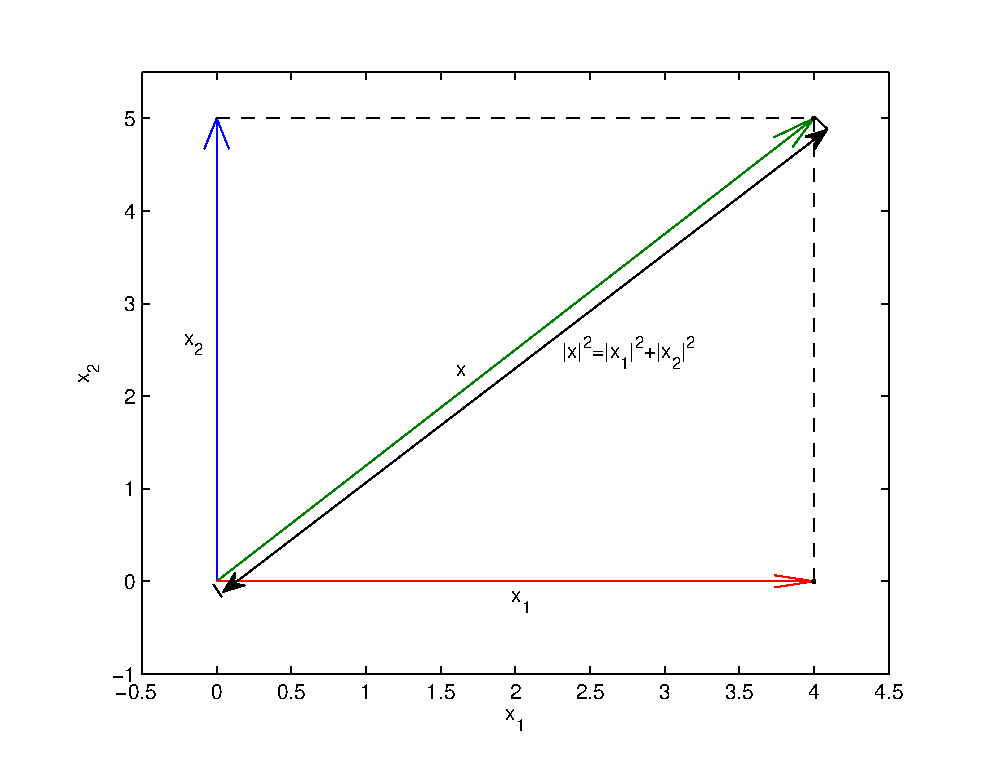
\includegraphics[width=12cm]{pitag.eps}
\bicaption{interpretación geométrica de la norma de un vector}{Geometrical interpretation of the norm of a vector.}
\label{fig:pitag}
\end{figure}
\begin{paracol}{2}
A partir de la norma de un vector es posible obtener una expresión alternativa para el producto escalar de dos vectores,
\switchcolumn
We can derive an alternative expression of the scalar product of two vector, using the vector norm
\end{paracol}
\begin{equation*}
a\cdot b=\Vert a \Vert \Vert b \Vert \cos \theta
\end{equation*}
\begin{paracol}{2}
Donde $\theta$ representa el ángulo formado por los dos vectores.
\switchcolumn
where $\theta$ is the angle between the two vectors.
\end{paracol}

\begin{flalign*}
&\mathwitch*_{i=0}^{\infty}\Xi_i(t)&     
\end{flalign*}

\begin{paracol}{2}
Aunque se trate de la manera más común de definir la norma de un vector, la norma 2 no es la única definición posible,

\emph{Norma 1:} Se define como la suma de los valores absolutos de los elementos de un vector,
\switchcolumn
Being the norm 2 the most common way to define a vector norm is by no means the only possible definition,

\emph{Norm 1:} defined as the sum of the absolute values of vector elements. 
\end{paracol}
\begin{equation*}
\Vert x \Vert_1 =\vert x_1\vert +\vert x_2 \vert\cdots \vert x_n\vert
\end{equation*}
\begin{paracol}{2}
\emph{Norma p:} Es una generalización de la norma 2,
\switchcolumn
\emph{P-Norm:} It is a generalization of the norm 2
\end{paracol}

\begin{equation*}
\Vert x \Vert_p =\sqrt[p]{\vert x_1^p\vert+\vert x_2^p\vert+\cdots \vert x_n^p\vert}=\left( \sum_{i=1}^n\vert x_i^p \vert \right)^\frac{1}{p}
\end{equation*}

\begin{paracol}{2}
\emph{Norma $\infty$:} se define como el mayor elemento del vector valor absoluto,
\switchcolumn
\emph{$\infty$ Norm:} The element with the largest absolute value
\end{paracol}

\begin{equation*}
\Vert x \Vert_\infty =max \left\lbrace \vert x_i\vert\right \rbrace 
\end{equation*}

\begin{paracol}{2}
\emph{Norma $-\infty$:} el menor elemento del vector en valor absoluto,
\switchcolumn
\emph{$-\infty$ Norm:} The element of the smallest absolute value. 
\end{paracol}
\begin{equation*}
\Vert x \Vert_{-\infty} =min \left\lbrace \vert x_i\vert\right \rbrace 
\end{equation*}
\begin{paracol}{2}
En Numpy la norma de un vector puede obtenerse mediante el comando \mintinline{python}{norm(v,p)}. La primera variable de entrada debe ser un vector y la segunda el tipo de norma que se desea calcular. Si se omite la segunda variable de entrada, el comando devuelve la norma 2. Para las normas $\infty\ \text{y} -\infty$ Se emplea el símbolo especial \mintinline{python}{inf} de Numpy. A continuación se incluyen varios ejemplo de utilización,
\switchcolumn
In Numpy the vector norm can be obtained using the command \mintinline{python}{norm(v,p)}. The first variable should be a vector and the second one represents the norm we want to calculate. If we leave out the second variable, the function returns norm 2 by default. For norms $\infty\ \text{y} \infty$ we use the symbol\mintinline{python}{inf} to represent the norm kind.
\end{paracol}

\begin{center}
    \begin{minipage}{.5\textwidth}
        \begin{minted}{python}
In [422]: a
Out[422]: array([1, 2, 3, 4])

In [423]: np.linalg.norm(a,1)
Out[423]: 10.0

In [424]: np.linalg.norm(a,2)
Out[424]: 5.477225575051661

In [425]: np.linalg.norm(a)
Out[425]: 5.477225575051661

In [426]: np.linalg.norm(a,4)
Out[426]: 4.337613136533361

In [427]: np.linalg.norm(a,np.inf)
Out[427]: 4.0

In [428]: np.linalg.norm(a,-np.inf)
Out[428]: 1.0
        \end{minted}
    \end{minipage}
\end{center}

\begin{paracol}{2}
En general, una norma se define como una función $\mathbb{R}^n \rightarrow \mathbb{R}$, que cumple,
\switchcolumn
In general, a norm can be define as functions $\mathbb{R}^n \rightarrow \mathbb{R}$, which satisfies,
\end{paracol}
\begin{align*}
&\Vert x\Vert \geq 0,\  \Vert x\Vert =0 \Rightarrow x=0\\
&\Vert x+y\Vert \leq \Vert x\Vert +\Vert y\Vert \\
&\Vert \alpha x\Vert = \vert \alpha \vert \Vert x\Vert ,\ \alpha \in \mathbb{R} 
\end{align*}

\begin{flalign*}
&&\reversemathwitch*    
\end{flalign*}

\begin{paracol}{2}
Llamaremos vectores unitarios $u$, a aquellos para los que se cumple que $\Vert u \Vert=1$.

Dos vectores $a$ y $b$ son ortogonales si cumplen que su producto escalar es nulo, $a^Tb=0 \Rightarrow  a\bot b$. Si además ambos vectores tienen módulo unidad, se dice entonces que los vectores son ortonormales.  Desde el punto de vista de su representación geométrica, dos vectores ortogonales, forman entre sí un ángulo recto.

\paragraph{Traza de una matriz.} La traza de una matriz cuadrada , se define como la suma de los elementos que ocupan su diagonal principal
\switchcolumn
Vectors $u$ with $\Vert u \Vert=1$ are called unitary vectors.

Two vectors $a$ and $b$ are orthogonal if their scalar product is zero, $a^Tb = 0 \Rightarrow a\bot b$. Besides, if the vectors have norm one them they are called orthonormal vectors. From the point of view of the geometrical representation, the angle between two orthogonal vectors is a square angle.

\paragraph{Matrix's trace.} The trace of a square matrix is the sum of the elements located in the matrix's main diagonal. 
\end{paracol}
\begin{gather*}
Tr(A)=\sum_{i=1}^na_{ii}\\
Tr\left(
\begin{pmatrix}
1& 4 & 4\\
2& -2 & 2\\
0& 3 & 6
\end{pmatrix}\right)=1-2+6=5
\end{gather*}

\begin{paracol}{2}
La traza de la suma de dos matrices cuadradas $A$ y $B$ del mismo orden, coincide con la suma de las trazas de $A$ y $B$,
\switchcolumn
The trace of the sum of two square, same dimension matrices $A$ and $B$ is equal to the sum of $A$ trace plus $B$ trace, 
\end{paracol}

\begin{equation*}
tr(A+B)=tr(A)+tr(B)
\end{equation*}

\begin{paracol}{2}
Dada una  matriz $A$ de dimensión $m\times n$  y una matriz $B$ de dimensión $n \times m$, se  cumple que,
\switchcolumn
For two matrices $A$ of dimensions $m\times n$ and $B$ of dimensions $n\times m$ is  always true that,
\end{paracol}

\begin{equation*}
tr(AB)=tr(BA)
\end{equation*}
\begin{paracol}{2}
En Python, puede obtenerse directamente el valor de la traza de una matriz $A$, mediante la función \mintinline{python}{np.trace(A)}. En este caso, se trata de un método asociado a cualquier array por lo que también puede expresarse como \mintinline{python}{A.trace()}  
\switchcolumn
In Numpy, the value of a matrix's trace can be calculated using the function \mintinline{python}{np.trace(A)}. In this case, the function is a method associated to any matrix and can be also expressed as \mintinline{python}{A.trace()}  
\end{paracol}

\begin{center}
\begin{minipage}{0.5\textwidth}
\begin{minted}{python}
In [197]: A = np.array([[1,2,3],[3,-2,3],[0,2,-1]])

In [198]: A
Out[198]: 
array([[ 1,  2,  3],
       [ 3, -2,  3],
       [ 0,  2, -1]])

In [199]: np.trace(A)
Out[199]: -2

In [200]: A.trace()
Out[200]: -2
\end{minted}
\end{minipage}
\end{center}


\begin{paracol}{2}
\paragraph{Determinante de una matriz.} 
En Numpy, el determinante de una matriz se calcula  empleando la función \mintinline{python}{det}, del submódulo \mintinline{python}{linalg}. Así, para calcular el determinante de la matriz $A$ del ejemplo anterior,
\switchcolumn
\paragraph{Matrix's determinant.} In Numpy, a matrix's determinant can be calculated using the function \mintinline{python}{det}, del submódulo \mintinline{python}{linalng}. We can calculate the determinant of matrix \mintinline{python}{A} of the previous example, 
\end{paracol}
\begin{center}
\begin{minipage}{0.5\textwidth}
\begin{minted}{python}
In [203]: np.linalg.det(A)
Out[203]: 20.000000000000007
\end{minted}
\end{minipage}
\end{center}

\begin{flalign*}
&\mathwitch*_{i=0}^{\infty}\Xi_i(t)&     
\end{flalign*}
\begin{paracol}{2}
El determinante de una matriz $A$, se representa habitualmente como $\vert A \vert$ o, en ocasiones como $det(A)$. Para poder definir el determinante de una matriz, necesitamos antes introducir una serie de conceptos previos. En primer lugar, si consideramos un escalar como una matriz de un solo elemento, el determinante  sería precisamente el valor de ese único elemento,
\switchcolumn
The determinant of a matrix, $A$ is usually represented as $\vert A\vert$ and occasionally as $det(A)$. To define the determinant of a matrix, we need first to establish some previous definitions. First, if we consider a scalar as a matrix of a single element, the determinant of the matrix is this single element.
\end{paracol}
\begin{equation*}
A=\begin{pmatrix}
a_{11}
\end{pmatrix} \rightarrow \vert A \vert =a_{11}
\end{equation*}
\begin{paracol}{2}
En álgebral lineal, se denomina menor primero, $M_{ij}$ de una matriz $A$, al determinate de la matriz que resulta de eliminar de la matriz $A$ la fila $i$ y la columna $j$. Por ejemplo,
\switchcolumn
In linear algebra, a first minor $M_{ij}$ of a square matrix $A$ is the determinant of the matrix obtained by removing simultaneously row $i$ and column $j$ of $A$. For instance, 
\end{paracol}

\begin{align*}
A=\begin{pmatrix}
1& 0& -2\\
3& -2& 3\\
0& 6& 5
\end{pmatrix},& \ 
M_{23}=det
\begin{pmatrix}
1& 0\\
0& 6
\end{pmatrix}\\
M_{32}=
det\begin{pmatrix}
1& -2\\
3& 3
\end{pmatrix},& \ 
M_{33}=
det\begin{pmatrix}
1& 0\\
3& -2
\end{pmatrix}\cdots
\end{align*}

\begin{paracol}{2}
 El  cofactor $C_{ij}$ de un elemento $a_{ij}$ de la matriz $A$, se define a partir del menor primero $M_{ij}$, que corresponde precísamenta a la fila y columna que contiene a $a_{ij}$,
 \switchcolumn
 We define the cofactor $C_{ij}$ of a matrix $A_{ij}$ element, $a_{ij}$, using the first minor $M_{ij}$ obtained removing the row and column $a_{ij}$ belongs to.
\end{paracol}
 
\begin{equation*}
C_{ij}=(-1)^{i+j} M_{ij}
\end{equation*}

\begin{paracol}{2}
Podemos ahora definir el determinante de una matriz $A$ cuadrada de orden $n$, empleando la fórmula de Laplace,
\switchcolumn
Now, we can define the determinant of a $n$ dimensional square matrix $A$, using the Laplace's formula, 
\end{paracol}
\begin{equation*}
\vert A \vert = \sum_{j=1}^n a_{ij}C_{ij}
\end{equation*}
\begin{paracol}{2}
o alternativamente,
\switchcolumn
or also as,
\end{paracol}

\begin{equation*}
\vert A \vert = \sum_{i=1}^n a_{ij}C_{ij}
\end{equation*}
\begin{paracol}{2}
En el primer caso, se dice que se ha desarrollado el determinante a lo largo de la fila $i$. En el segundo caso, se dice que se ha desarrollo a lo largo de la columna $j$.

 La fórmula de Laplace obtiene el determinante de una matriz de orden $n\times n$ a partir del cálculo de los menores complementarios de los elementos de una fila o columna; los determinates the $n$ matrices de orden $(n-1)\times (n-1)$. A su vez, podríamos calcular cada menor complementario, aplicando la fórmula de Laplace y así sucesivamente hasta llegar a matrices de orden $2\times 2$. Para una matriz $2\times 2$, si desarrollamos por la primera fila obtenemos su determinante como,
\switchcolumn
In the first case, we say that we develop the determinant along the row $i$. In the second one, we say that we have developed the determinant along the column $j$

Laplace's formula gets the determinant of a Matrix of dimensions $n\times n$ using the first minors of a matrix row or column, i.e. the determinants of $n$ matrix of order $(n-1)\times (n-1)$. In turn, we can calculate each minor using Laplace's formula and so on, till we arrive at matrices of dimension $2\times 2$. We obtain the determinant of a $2\times 2$ matrix developing it along its first row,      

\end{paracol}

\begin{align*}
A&=\begin{pmatrix}
a_{11}& a_{12}\\
a_{21}& a_{22}
\end{pmatrix}\\
\vert A \vert & =\sum_{j=1}^2a_{1j}C_{1j} =a_{11}C_{11}+a_{12}C_{12}\\
 &=a_{11}(-1)^{1+1}\vert M_{11}\vert +a_{12}(-1)^{1+2}\vert M_{12}\vert \\
 &=-a_{11}a_{22}+a_{12}a_{21}\\
\end{align*}

\begin{paracol}{2}
y si desarrollamos por la segunda columna,
\switchcolumn
And if  we develop using the secon column,
\end{paracol}
\begin{align*}
A&=\begin{pmatrix}
a_{11}& a_{12}\\
a_{21}& a_{22}
\end{pmatrix}\\
\vert A \vert & =\sum_{j=1}^2a_{i2}C_{i2} =a_{12}C_{12}+a_{22}C_{22}\\
 &=a_{12}(-1)^{1+2}\vert M_{12}\vert +a_{22}(-1)^{2+2}\vert M_{22}\vert \\
 &=-a_{12}a_{21}+a_{22}a_{12}\\
\end{align*}

\begin{paracol}{2}
Para una matriz de dimensión arbitraria $n\times n$, el determinante se obtiene aplicando recursivamente la fórmula de Laplace,
\switchcolumn
For a matrix of arbitrary dimension we obtain the determinant using the Laplace's formula recursively,
\end{paracol}

\begin{align*}
&\vert A  \vert = \sum_{j=1}^na_{ij}C_{ij} =\sum_{j=1}^na_{ij}(-1)^{i+j} \left \vert M_{ij}^{(n-1)\times(n-1)} \right \vert \\
&\left \vert M_{ij}^{(n-1)\times(n-1)} \right \vert = \sum_{k=1}^{n-1}m_{lk}C_{lk} =\sum_{k=1}^{n-1}m_{lk}(-1)^{l+k} \left \vert M_{lk}^{(n-2)\times (n-2)} \right \vert\\
&\vdots \\
&\left \vert M_{st}^{1\times 1}\right \vert=(-1)^{s+t}m_{st} 
\end{align*}
\begin{paracol}{2}
Así, por ejemplo, podemos calcular el determinante de la matriz,
\switchcolumn
For instance, we can calculate the determinant of the following matrix,
\end{paracol}
\begin{equation*}
A=\begin{pmatrix}
1& 0& -2\\
3& -2& 3\\
0& 6& 5
\end{pmatrix}
\end{equation*}
\begin{paracol}{2}
desarrollándolo por los elementos de la primera columna, como,
\switchcolumn
Developing by the first column elements,
\end{paracol}
\begin{align*}
\left\vert A \right\vert =& 1\cdot (-1)^2\cdot 
\left\vert \begin{matrix}
-2& 3\\ 
6& 5
\end{matrix} \right\vert + 3\cdot (-1)^3\cdot
\left\vert \begin{matrix}
0& -2\\ 
6& 5
\end{matrix} \right\vert+ 0\cdot (-1)^4 \cdot 
\left\vert \begin{matrix}
0& -2\\ 
-2& -3
\end{matrix} \right\vert \\
=& 1\cdot (-1)^2\cdot \left[ (-2)\cdot 5 - 6\cdot 3 \right] +3\cdot (-1)^3\cdot  \left[ 0\cdot 5 - 6\cdot (-2)\right] + 0\cdot (-1)^4 \cdot \left[ 0\cdot 3 - (-2)\cdot (-2)\right]= -64
\end{align*}

\begin{paracol}{2}
Podemos programar en Python una función recursiva\footnote{El método no es especialmente eficiente pero ilustra el uso de funciones recursivas.} que calcule el determinante de una matriz de dimensiones $n\times n$.
\switchcolumn
We can now program a recursive function\footnote{The method is not particularly efficient but it helps to show the use of recursive functions} to calculate the determinant of any $n\times n$ dimensions.
\end{paracol}

\inputminted[
frame=lines,
framesep=2mm,
baselinestretch=1.2,
%bgcolor=LightGray,
label=determinante.py,
fontsize=\footnotesize,
linenos
]{python}{./codigos/Algebra/codigo_abierto/determinante.py}
\begin{flalign*}
&&\reversemathwitch*
\end{flalign*}
\begin{paracol}{2}
Entre las propiedades de los determinantes, destacaremos las siguientes,
\begin{enumerate}
\item El determinante del producto de un escalar $a$ por una matriz $A$ cumple,
\begin{equation*}
\left\vert a\cdot A \right\vert =a^n\cdot \vert A \vert
\end{equation*}
\item El determinante de una matriz es igual al de su traspuesta,
\begin{equation*}
\vert A \vert =\left\vert A^T \right\vert
\end{equation*}

\item El determinante del producto de dos matrices es igual al producto de los determinantes,
\begin{equation*}
\left\vert A_{n\times n} \cdot  B_{n\times n} \right\vert = \left\vert A_{n\times n} \right\vert \cdot \left\vert B_{n\times n} \right\vert 
\end{equation*}
\end{enumerate}

Una matriz es singular si su determinante es cero.

El rango de una matriz $A$ se define como el tamaño de la submatriz más grande dentro de $A$, cuyo determinante es distinto de cero. Así por ejemplo la matriz,
\switchcolumn
Among determinants' properties we will point out the following ones,
\begin{enumerate}
	\item The determint of a escalar $a$ by a  matrix $A$ is,
	\begin{equation*}
		\left\vert a\cdot A \right\vert =a^n\cdot \vert A \vert
	\end{equation*}
	\item The determinant of a matrix traspose equals the determinant of the matrix,
	\begin{equation*}
		\vert A \vert =\left\vert A^T \right\vert
	\end{equation*}
	
	\item The determinant of a matrix product equals the product of their determinants,
	\begin{equation*}
		\left\vert A_{n\times n} \cdot  B_{n\times n} \right\vert = \left\vert A_{n\times n} \right\vert \cdot \left\vert B_{n\times n} \right\vert 
	\end{equation*}
\end{enumerate}

A singular matrix is a square matrix whose determinant is zero.

The rank of a matrix $A$ is the size of the largest submatrix, inside $A$, whose determinant is non-zero. For instance,  
\end{paracol}
\begin{equation*}
A=\begin{pmatrix}
1& 2& 3\\
4& 5& 6\\
7& 8& 9
\end{pmatrix} \rightarrow \vert A \vert =0
\end{equation*}
\begin{paracol}{2}
Es una matriz singular y su rango es dos,
\switchcolumn
is a singular matrix, and its rank is 2,    
\end{paracol}

\begin{equation*}
\left \vert \begin{matrix}
1& 2\\
4& 5
\end{matrix} \right \vert=-3 \neq 0 \Rightarrow r(A)=2
\end{equation*}
\begin{paracol}{2}
Para una matriz cuadrada no singular, su rango coincide con su dimensión.

En Numpy se puede obtener el rango de una  matriz mediante el comando \mintinline{python}{matrix_rank},
\switchcolumn
For a non-singular square matrix, its rank meets its dimension.

In Numpy, we can obtain the rank of a matrix using the comand \mintinline{python}{matrix_rank},  
\end{paracol}
\begin{center}
\begin{minipage}{0.5\textwidth}
\begin{minted}{python}
In [395]: A
Out[395]: 
array([[1, 2, 3],
       [4, 5, 6],
       [7, 8, 9]])

In [396]: np.linalg.matrix_rank(A)
Out[396]: 2
\end{minted}
\end{minipage}
\end{center}
\begin{paracol}{2}
\paragraph{Inversión.} Dada una matriz cuadrada no singular $A$ de dimension $n$ existe una única matriz $A^{-1}$ de dimension $n$ que cumple,
\begin{equation*}
A\cdot A^{-1}=I_{n\times n}
\end{equation*}
Donde $I_{n\times n}$ es la matriz indentidad de dimensión $n$.
La matriz $A^{-1}$ recibe el nombre de matriz inversa de $A$, y  en numpy puede calcularse a partir de $A$ como \mintinline{python}{np.linalg.inv(A)}, ó \mintinline{python}{np.linalg.matrix_power(A,-1)}
En el segundo caso, estamos empleando la función, del submódulo linalg de numpy, \mintinline{python}{matrix.power(A,n)} que permite calcular el resultado de elevar una matriz a una pontencia $A^n$.
\switchcolumn
\paragraph{Inversion.} For a square non-singular matrix $A$ of dimension $n$ there is a unique matrix $A^{-1}$ of dimension $n$ that satisfies,
\begin{equation*}
	A\cdot A^{-1}=I_{n\times n}
\end{equation*}
Where $I_{n\times n}$ is the identity matrix of dimension $n$. The matrix $A^{-1}$ is called the inverse matrix of $A$, and we can calculate it in Numpy appliying the comands  \mintinline{python}{np.linalg.inv(A)}, ó \mintinline{python}{np.linalg.matrix_power(A,-1)} to the matrix $A$.
In the second case, we are using the function \mintinline{python}{matrix.power(A,n)} which allows us to calculate the result to raise a natrix to a power $A^n$. 
\end{paracol}
\begin{center}
\begin{minipage}{0.7\textwidth}
\begin{minted}{python}
In [409]: B = np.linalg.inv(A)

In [410]: B
Out[410]: 
array([[ 1.29166667, -0.58333333, -0.04166667],
       [ 0.58333333, -0.16666667, -0.08333333],
       [-0.48611111,  0.30555556,  0.06944444]])

In [411]: B @ A
Out[411]: 
array([[ 1.00000000e+00, -5.55111512e-17, -1.11022302e-16],
       [ 0.00000000e+00,  1.00000000e+00, -1.11022302e-16],
       [ 0.00000000e+00,  0.00000000e+00,  1.00000000e+00]])

In [412]: np.linalg.matrix_power(A,-1)
Out[412]: 
array([[ 1.29166667, -0.58333333, -0.04166667],
       [ 0.58333333, -0.16666667, -0.08333333],
       [-0.48611111,  0.30555556,  0.06944444]])
\end{minted}
\end{minipage}
\end{center}
\begin{flalign*}
&\mathwitch*_{i=0}^{\infty}\Xi_i(t)&     
\end{flalign*}
\begin{paracol}{2}
La inversa de una matriz puede obtenerse a partir de la expresión,
\switchcolumn
A matrix inverse can be calculate using the following expression,
\end{paracol}
\begin{equation*}
A^{-1}=\frac{1}{\vert A \vert}[adj(A)]^T
\end{equation*}
\begin{paracol}{2}
Donde $adj(A)$ es la matriz adjunta de $A$, que se obtiene sustituyendo cada elemento $a_{ij}$ de $A$, por su cofactor $C_{ij}$. A continuación incluimos el código en Python de una función, \mintinline{python}{inver}, que calcula la inversa de una matriz. La función \mintinline{python}{inver} llama a su vez a la función \mintinline{python}{dumbdet} descrita más arriba, por lo que debemos importar el módulo \mintinline{python}{determinante} en el módulo en que vamos a crear la función \mintinline{python}{inver}.
\switchcolumn 
Where $adj(A)$ is the adjugate matrix of $A$, which can be obtained replacing each element $a_{ij}$ of $A$ by its cofactor $C_{ij}$. Next, We include the Python code of a function, \mintinline{python}{inver}, to calculate the inverse of a matrix. The function \mintinline{python}{inver}, in turn,  calls the function \mintinline{python}{dumbdet}. Therefore, we must need to import the module \mintinline{python}{determinante} in the module where we will create the funtion \mintinline{python}{inver} 
\end{paracol}
\inputminted[
frame=lines,
framesep=2mm,
baselinestretch=1.2,
%bgcolor=LightGray,
label=inversa.py,
fontsize=\footnotesize,
linenos
]{python}{./codigos/Algebra/codigo_abierto/inversa.py}

\begin{flalign*}
&&\reversemathwitch*
\end{flalign*}

\begin{paracol}{2}
Algunas propiedades relacionadas con la inversión de matrices son,
\begin{enumerate}
\item Inversa del producto de dos matrices,
\begin{equation*}
(A\cdot B)^{-1}=B^{-1}\cdot A^{-1}
\end{equation*}

\item Determinante de la inversa,
\begin{equation*}
\left\vert A^{-1} \right\vert = \vert A \vert ^{-1}
\end{equation*}

\item Una matriz es ortogonal si su inversa coincide con su transpuesta,
\begin{equation*}
A^{-1}=A^T
\end{equation*}
\end{enumerate}
\end{paracol}

\begin{table}
\bicaption{Algunas funciones matemáticas en Numpy de uso frecuente}{frecuently used mathematical functions included in Numpy}
\label{tabfun}
\begin{tabular}{c|c|c|c}
Tipo&Nombre&variables&función matemática\\
Type&Name&variables&funcion matemática\\
\hline
\hline

Trigonométricas&\multirow{2}{*}{cos}&\multirow{2}{4em}{y=cos(x)}&coseno de un ángulo en radianes\\
Trigonometric& & & Cosine of angle in radians\\
\hline
Trigonometricas&\multirow{2}{*}{sin}&\multirow{2}{4em}{y=sin(x)}&seno de un ángulo en radianes\\
Trigonometric& & &Sine of an angle in radians\\
\hline
Trigonométricas&\multirow{2}{*}{tan}&\multirow{2}{4em}{y=tan(x)}&tangente de un ángulo en radianes\\
Trigonometric & & &Tangent of an angle in radians\\
\hline
Trigonométricas &...&y=arc...(x)&inversa de una función trigonométrica\\
Trigonometric &arcsin&y=arcsin(x)& Inverse of a trigonometric function\\
\hline
\hline
Exponencial&\multirow{2}{*}{exp}&\multirow{2}{*}{y=exp(x)}&\multirow{2}{*}{$e^x$}\\
Exponential& & & \\
\hline
Exponencial&\multirow{2}{*}{log}&\multirow{2}{*}{y=log(x)}&logaritmo natural\\
Exponential & & & Natural logarithm\\
\hline
Exponencial&\multirow{2}{*}{log10}&\multirow{2}{*}{log10(x)}&logaritmo en base 10\\
Exponential& & & Basis 10 logarithm\\
\hline
Exponencial&\multirow{2}{*}{sqrt}&\multirow{2}{*}{y=sqrt(x)}&\multirow{2}{*}{$\sqrt{x}$}\\
Exponential& & & \\
\hline
\hline
Redondeo&\multirow{2}{*}{ceil}&\multirow{2}{*}{y=ceil(x)}& redondeo hacia $+\infty$\\
Rounding& & & rounding towards $+\infty$\\
\hline
Redondeo&\multirow{2}{*}{floor}&\multirow{2}{*}{y=floor(x)}&redondeo hacia $-\infty$\\
Rounding& & & rounding towards $-\infty$ \\
\hline
Redondeo&\multirow{2}{*}{rint}&\multirow{2}{*}{y=rint(x)}&redondeo al entero más próximo\\
Rounding& & & rounding towards the nearest integer\\
\hline
Redondeo&\multirow{2}{*}{fix}&\multirow{2}{*}{y=fix(x)}&redondeo hacia $0$\\
Rounding& & & rounding towards $0$\\
\hline
Redondeo&\multirow{2}{*}{mod}&\multirow{2}{*}{r=mod(x,y)}&resto de la división entera de y entre x\\
Rounding& & & remainder after integer division\\
\hline
\hline
Módulos&\multirow{2}{*}{norm}&\multirow{2}{*}{y=norm(x)}& módulo de un vector x\\
Norms & & & Norm of a vector\\
\hline
Módulos&\multirow{2}{*}{abs}&\multirow{2}{*}{y=abs(x)}&valor absoluto de x\\
Norms & & & Absolute value of x\\
\hline
Módulos&\multirow{2}{*}{sign}&\multirow{2}{*}{y=sign(x)}&función signo; 1 si x $>$ 0, -1 si x $<$ 0, 0 si x=0\\
Norms & & &sign function; 1 if x $>$ 0, -1 if x $<$ 0, 0 if x=0\\ 
\end{tabular}
\end{table}

\begin{paracol}{2}
\subsection{Funciones incluidas en\\ Num\-py.}\index{Funciónes! Funciones incluidas en Numpy} 
Numpy incluye un gran número de funciones. Muchas de ellas  están pensadas para ser aplicadas a arrays o a variables numéricas indistintamente. En el primer caso, la función se aplica elemento a elemento y el resultado es un array con las mismas dimensiones que el original. 

En la tabla \ref{tabfun}, se incluyen algunos ejemplos de las funciones matemáticas más corrientes. No están todas. Para obtener una visión más completa de las funciones disponibles se aconseja acudir a la documntacion de Numpy.
El uso de estas funciones es directo, por ejemplo, el siguiente código calcula la exponencial de los elementos de una matriz,
\end{paracol}

\begin{center}
    \begin{minipage}{0.5\textwidth}
        \begin{minted}{python}
In [1]: import numpy as np

In [2]: A = np.array([[1,2],[2,0],[3,5]])

In [3]: A
Out[3]: 
array([[1, 2],
       [2, 0],
       [3, 5]])

In [4]: np.exp(A)
Out[4]: 
array([[  2.71828183,   7.3890561 ],
       [  7.3890561 ,   1.        ],
       [ 20.08553692, 148.4131591 ]])
        \end{minted}
    \end{minipage}
\end{center}

\begin{paracol}{2}
\section{Operadores vectoriales}\label{opvect}
En esta sección vamos a estudiar el efecto de las operaciones matriciales, descritas en la sección anterior, sobre los vectores. Empecemos por considerar el producto por un escalar $\alpha \cdot a$. El efecto fundamental es modificar el módulo del vector,
\end{paracol}
\begin{equation*}
\alpha \cdot \begin{pmatrix}
a_1\\
a_2\\
a_3
\end{pmatrix}=
\begin{pmatrix}
\alpha a_1\\
\alpha a_2\\
\alpha a_3
\end{pmatrix}\rightarrow \vert \vert \alpha \cdot a \vert \vert =\sqrt{\alpha ^2a_1^2+\alpha ^2a_2^2+\alpha ^2a_3^2}=\vert \alpha \vert  \sqrt{a_1^2+a_2^2+a_3^2}=\vert \alpha \vert \cdot \vert \vert a \vert \vert
\end{equation*}
\begin{paracol}{2}
Gráficamente, si $alpha$ es un número positivo y mayor que la unidad, el resultado del producto será un vector más largo que $a$ con la misma dirección y sentido. Si por el contrario, $\alpha$ es menor que la unidad, el vector resultante será más corto que $a$. Por último si se trata de un número negativo, a los resultados anteriores se añade el cambio de sentido con respecto a $a$. La figura \ref{fig:vmod} muestra gráficamente un ejemplo  del producto de un vector por un escalar.
\end{paracol}
\begin{figure}[h]
\centering
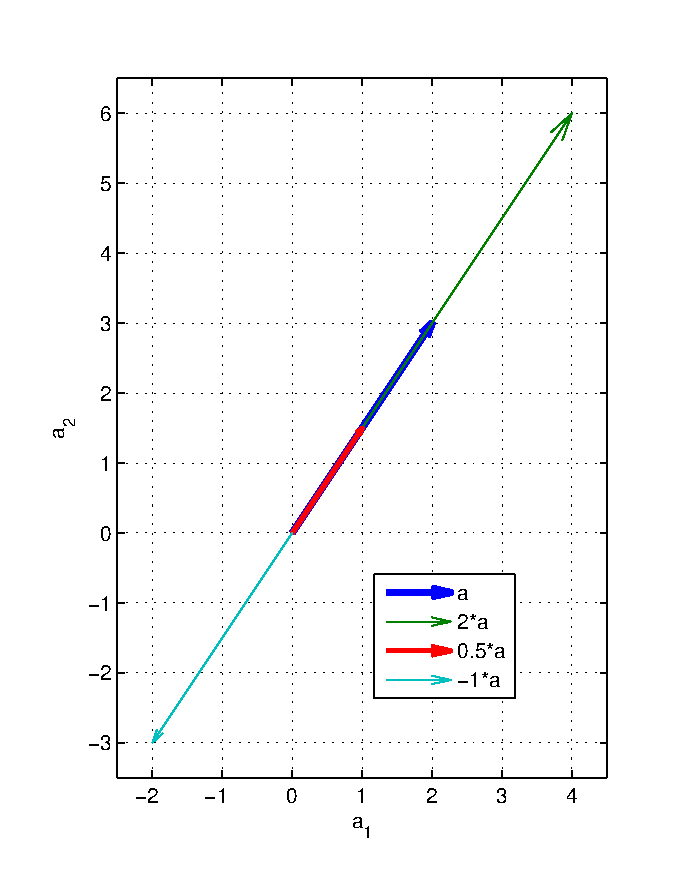
\includegraphics[width=7cm]{vmod.eps}
\caption{efecto del producto de un escalar por un vector}
\label{fig:vmod}
\end{figure}
\begin{paracol}{2}
\paragraph{Combinación lineal.} Combinando la suma de vectores, con el producto por un escalar, podemos generar nuevos vectores, a partir de otros, el proceso se conoce como combinación lineal,
\end{paracol}
\begin{equation*}
c=\alpha \cdot a + \beta \cdot b + \cdots +\theta z
\end{equation*}
\begin{paracol}{2}
Así el vector $c$ sería el resultado de una combinación  lineal de los vectores $a, b \cdots z$. 
Dado un conjunto de vectores, se dice que son linealmente independientes entre sí, si no es posible poner a unos como combinación lineal de otros,
\end{paracol}
\begin{equation*}
\alpha \cdot a + \beta \cdot b + \cdots +\theta z=0 \Rightarrow \alpha =\beta =\cdots =\theta =0
\end{equation*}

\begin{paracol}{2}
Es posible expresar cualquier vector de dimensión $n$ como una combinación lineal de $n$ vectores linealmente independientes.

Supongamos $n=2$, cualquier par de vectores que no estén alineados, pueden generar todos los vectores de dimensión $2$ por ejemplo,
\end{paracol}

\begin{equation*}
\begin{pmatrix}
x_1\\
x_2
\end{pmatrix}=
\alpha \begin{pmatrix}
1\\
2
\end{pmatrix}+\beta \begin{pmatrix}
-1\\
1
\end{pmatrix}
\end{equation*}

La figura \ref{fig:clineal} muestra gráficamente estos dos vectores y algunos de los vectores resultantes de combinarlos linealmente.

\begin{figure}[h]
\centering
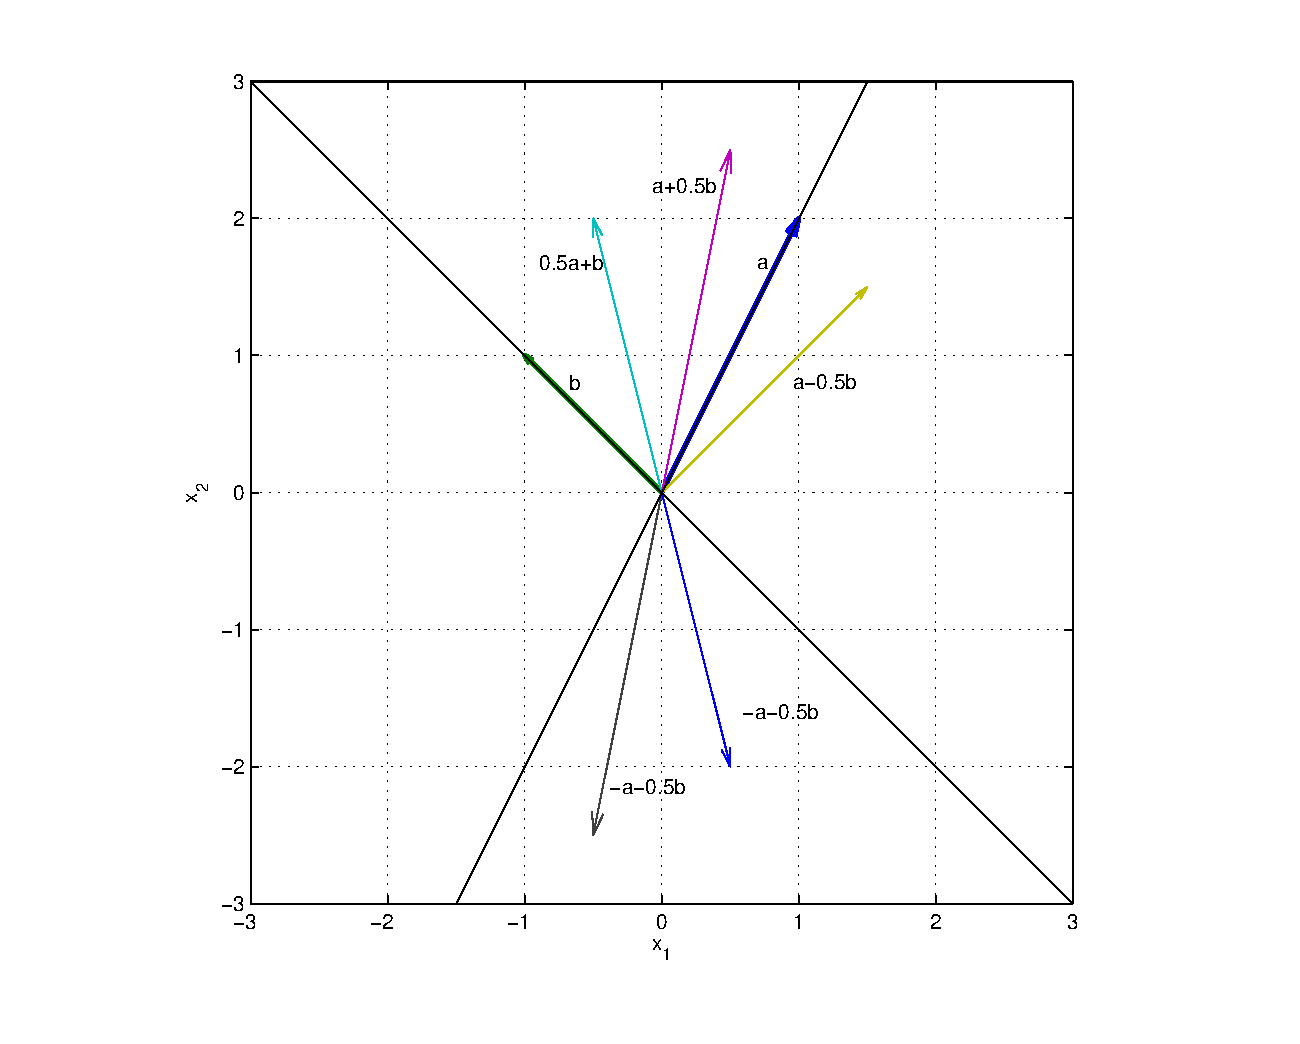
\includegraphics[width=10cm]{clineal.eps}
\caption{Representación gráfica de los vectores $a=(1,2)
$, $b=(-1,1)
$ y algunos vectores, combinación lineal de $a$ y $b$.}
\label{fig:clineal}
\end{figure}
\begin{paracol}{2}
Si tomamos como ejemplo $n=3$, cualquier conjunto de vectores que no estén contenidos en el mismo plano, pueden generar cualquier otro vector de dimensión $3$. Por ejemplo,
\end{paracol}
\begin{equation*}
\begin{pmatrix}
x_1\\
x_2\\
x_3
\end{pmatrix}=\alpha \begin{pmatrix}
1\\
-2\\
1
\end{pmatrix}+ \beta \begin{pmatrix}
2\\
0\\
-1
\end{pmatrix}+ \gamma \begin{pmatrix}
-1\\
1\\
1
\end{pmatrix}
\end{equation*}
\begin{paracol}{2}
La figura \ref{fig:clin3} muestra gráficamente estos tres vectores y el vector resultante de su combinación lineal, con $\alpha=1$, $\beta=-0.5$ y $\gamma=1$.  Es fácil ver a partir de la figura que cualquier otro vector de dimensión $3$ que queramos construir puede obtenerse a partir de los vectores $a$, $b$ y $c$.
\end{paracol}
\begin{figure}[h]
\centering
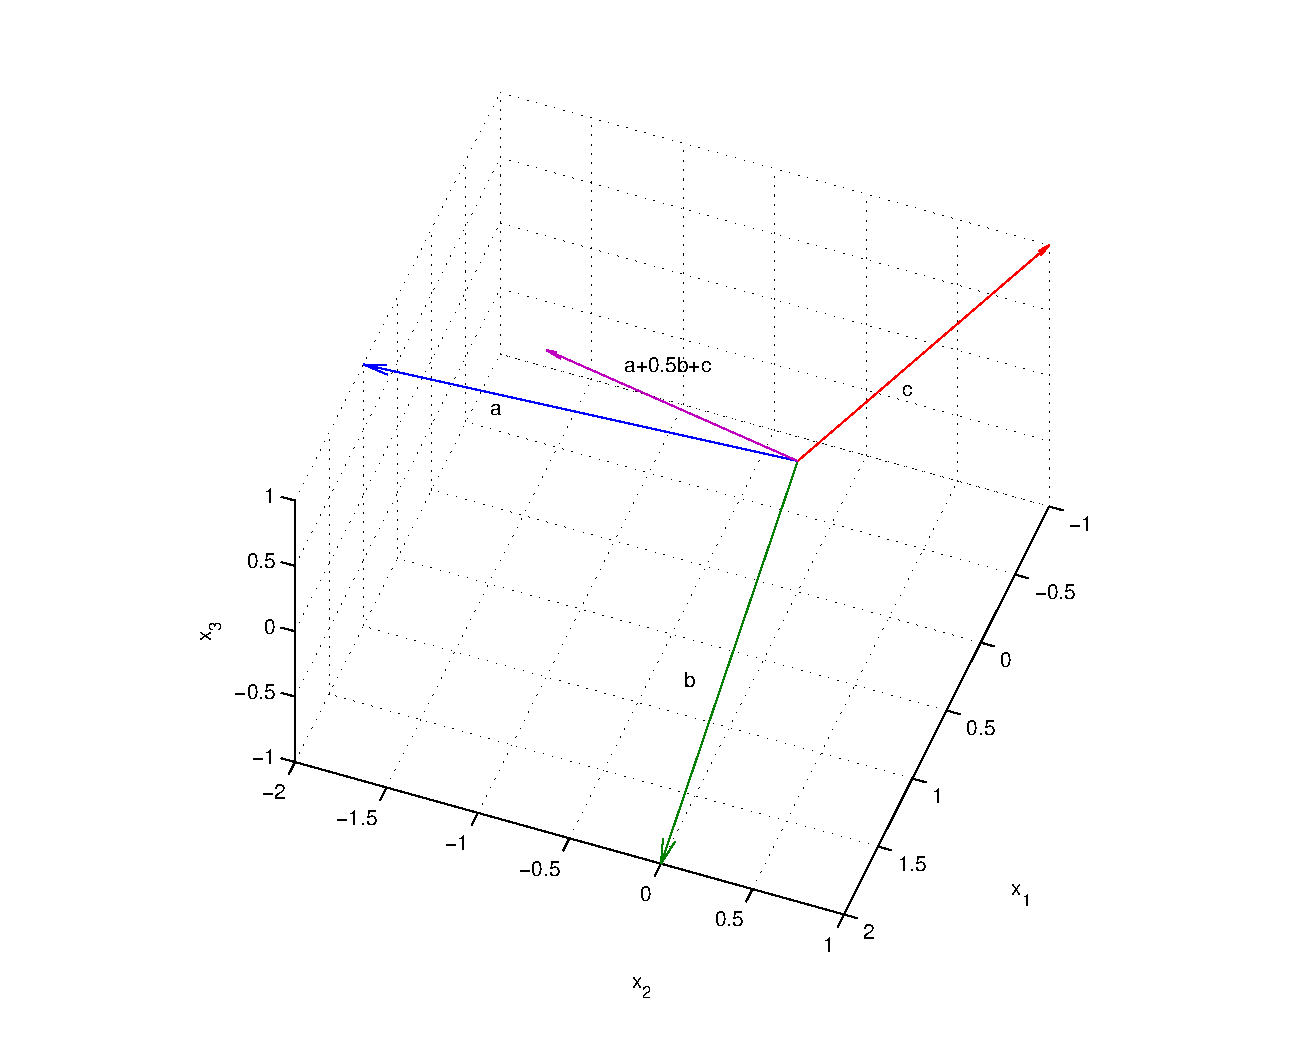
\includegraphics[width=12cm]{clin3.eps}
\caption{Representación gráfica de los vectores $a=(1,-2,1)
$, $b=(2,0,-1)$, $c=(-1,1,1)$ y del vector $a-b+c$.}
\label{fig:clin3}
\end{figure}

\begin{paracol}{2}
\paragraph{Espacio vectorial y  bases del espacio vectorial.} El conjunto de los vectores de dimensión $n$ (matrices de orden $n\times 1$), junto con la suma vectorial y el producto por un escalar, constituye  un  \emph{espacio vectorial} de dimensión $n$.

 Como acabamos de ver, es posible obtener cualquier vector de dicho espacio vectorial a partir de $n$ vectores linealmente independientes del mismo. Un conjunto de $n$ vectores linealmente independientes de un espacio vectorial de dimensión $n$ recibe el nombre de base del espacio vectorial. En principio es posible encontrar infinitas bases distintas para un espacio vectorial de dimensión $n$. Hay algunas particularmente interesantes,
 
 \subparagraph{Bases ortogonales.} Una base ortogonal es aquella en que todos sus vectores son ortogonales entre sí , es decir cumple que su producto escalar es $b^i\cdot b^j=0, i\neq j$. Donde  $b^i$ representa el \emph{i-ésimo} vector de la base, $\mathcal{B}=\left\lbrace b^1, b^2, \cdots, b^n  \right\rbrace $ .
 
 \subparagraph{Bases ortonormales.} Una base ortonormal, es una base ortogonal en la que, además, los vectores de la base tienen módulo $1$. Es decir, $b^i\cdot b^j=0, i\neq j$ y  $b^i\cdot b^j=1, i = j$. Un caso particularmente útil de base ortonormal es la base canónica, formada por los vectores, 
\end{paracol}

\begin{equation*}
\mathcal{C}=\left\lbrace c^1=\begin{pmatrix}
1\\
0\\
0\\
\vdots \\
0
\end{pmatrix}, c^2=\begin{pmatrix}
0\\
1\\
0\\
\vdots \\
0
\end{pmatrix},
\cdots
c^{n-1}=\begin{pmatrix}
0\\
0\\
\vdots \\
1\\
0
\end{pmatrix},
c^n=\begin{pmatrix}
0\\
0\\
\vdots \\
0\\
1
\end{pmatrix} \right\rbrace
\end{equation*} 
\begin{paracol}{2}
Podemos considerar las componentes de cualquier vector como los coeficientes de la combinación lineal de la base canónica que lo representa,
\end{paracol}
\begin{equation*}
a=\begin{pmatrix}
a_1\\
a_2\\
\cdots  \\
a_{n-1}\\
a_n
\end{pmatrix} =a_1\cdot \begin{pmatrix}
1\\
0\\
0\\
\vdots \\
0
\end{pmatrix}+a_2 \cdot  \begin{pmatrix}
0\\
1\\
0\\
\vdots \\
0
\end{pmatrix}+
\cdots +
a_{n-1}\cdot \begin{pmatrix}
0\\
0\\
\vdots \\
1\\
0
\end{pmatrix}+
a_n\cdot \begin{pmatrix}
0\\
0\\
\vdots \\
0\\
1
\end{pmatrix}
\end{equation*}

\begin{paracol}{2}
Por extensión, podemos generalizar este resultado a cualquier otra base, es decir podemos agrupar en un vector los coeficientes de la combinación lineal de los vectores de la base que lo generan. Por ejemplo, si construimos, para los vectores de dimensión $3$ la base,
\end{paracol}

\begin{equation*}
\mathcal{B}=\left\lbrace \begin{pmatrix}
1\\
2\\
0
\end{pmatrix}, \begin{pmatrix}
-1\\
0\\
2
\end{pmatrix}, \begin{pmatrix}
1\\
-1\\
1
\end{pmatrix} \right\rbrace
\end{equation*} 
\begin{paracol}{2}
Podemos entonces representar un vector en la base $\mathcal{B}$ como,
\end{paracol}

\begin{equation*}
\alpha \cdot \begin{pmatrix}
1\\
2\\
0
\end{pmatrix}+\beta \cdot \begin{pmatrix}
-1\\
0\\
2
\end{pmatrix}+ \gamma \cdot \begin{pmatrix}
1\\
-1\\
1
\end{pmatrix} \rightarrow a^{\mathcal{B}}=\begin{pmatrix}
\alpha \\
\beta \\
\gamma
\end{pmatrix}
\end{equation*} 
\begin{paracol}{2}
Donde  estamos empleando el superíndice $^{\mathcal{B}}$, para indicar que las componentes del vector $a$ están definidas con respecto a la base $\mathcal{B}$.

Así por ejemplo el vector,
\end{paracol} 
\begin{equation*}
a^{\mathcal{B}}=\begin{pmatrix}
1.125\\
0.375\\
0.75
\end{pmatrix}
\end{equation*}
\begin{paracol}{2}
Tendría en la base canónica las componentes,
\end{paracol}
\begin{equation*}
a^{\mathcal{B}}=\begin{pmatrix}
1.125\\
0.375\\
0.75
\end{pmatrix} \rightarrow a= 1.125 \cdot \begin{pmatrix}
1\\
2\\
0
\end{pmatrix}+0.375 \cdot \begin{pmatrix}
-1\\
0\\
2
\end{pmatrix}+ 0.75 \cdot \begin{pmatrix}
1\\
-1\\
1
\end{pmatrix} =\begin{pmatrix}
1.5\\
1.5 \\
1.5
\end{pmatrix}
\end{equation*}

\begin{paracol}{2}
La figura \ref{fig:base1}, muestra gráficamente la relación entre los vectores de la base canónica $\mathcal{C}$, los vectores de la base $\mathcal{B}$, y el vector $a$, cuyas componentes se han representado en ambas bases.

Podemos aprovechar el producto de matrices para obtener las componentes en la base canónica $\mathcal{C}$ de un vector representado en una base cualquiera $\mathcal{B}$. Si agrupamos los vectores de la base $\mathcal{B}$, en una matriz $B$,
\end{paracol}
\begin{figure}[h]
\centering
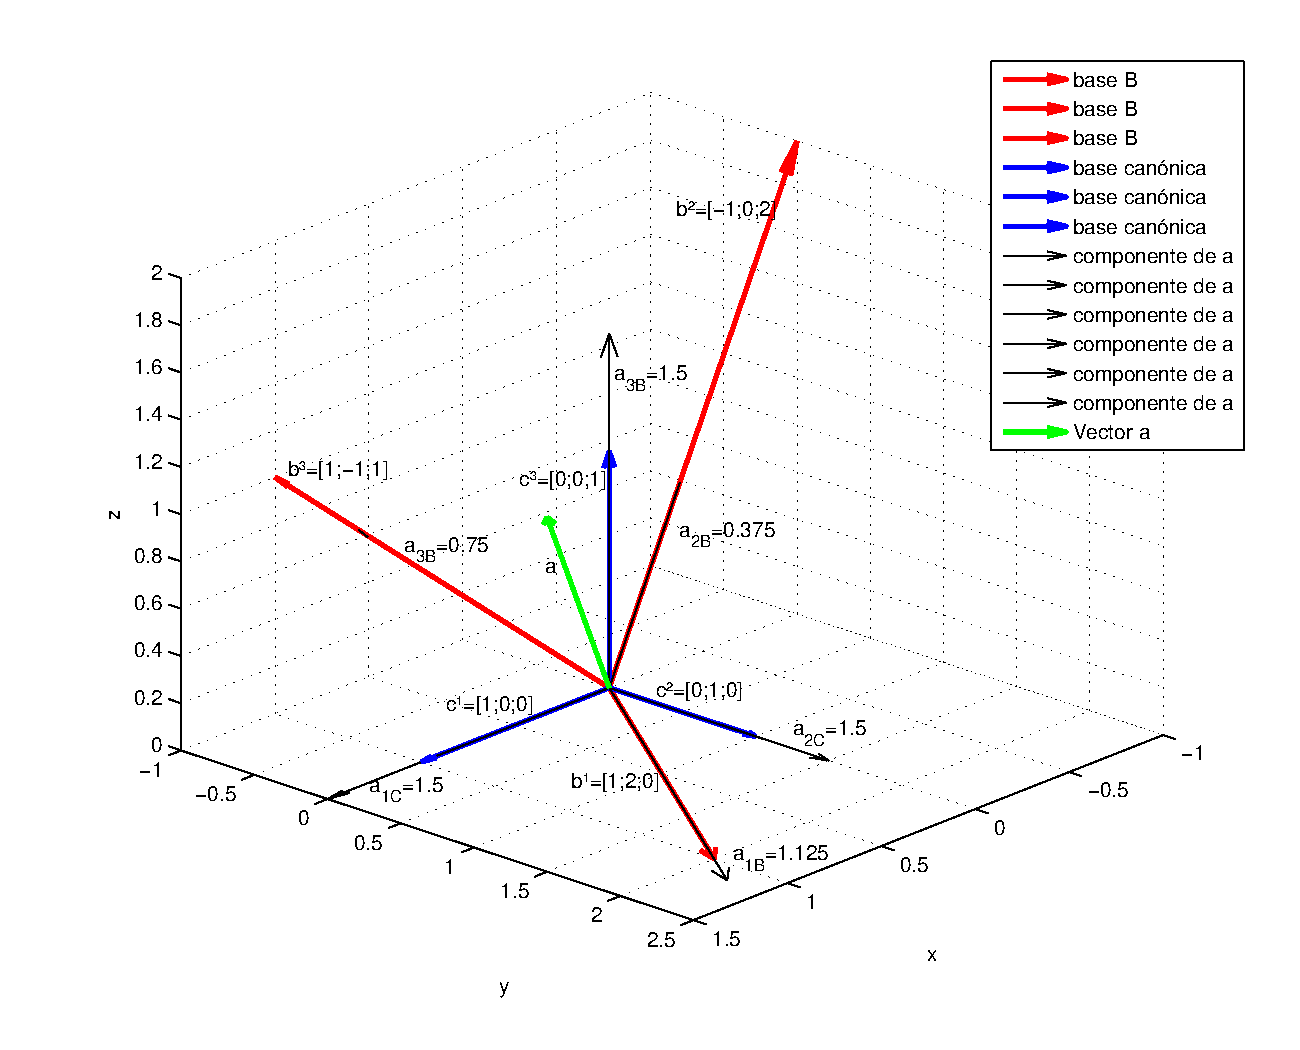
\includegraphics[width=15cm]{base1.eps}
\caption{Representación gráfica del vector $a$, en las base canónica $\mathcal{C}$ y en la base $\mathcal{B}$}
\label{fig:base1}
\end{figure}

\begin{equation*}
\mathcal{B}=\left\lbrace b^1=\begin{pmatrix}
b_{11}\\
b_{21}\\
b_{31}\\
\vdots \\
b_{n1}
\end{pmatrix},b^2=\begin{pmatrix}
b_{12}\\
b_{22}\\
b_{32}\\
\vdots \\
b_{n2}
\end{pmatrix},
\cdots
b^n=\begin{pmatrix}
b_{1n}\\
b_{2n}\\
\vdots \\
b_{(n-1)n}\\
b_{nn}
\end{pmatrix} \right\rbrace \rightarrow
B=\begin{pmatrix}
b_{11}&b_{12}& \cdots & b_{1n}\\
b_{21}&b_{22}& \cdots & b_{2n}\\
b_{31}&b_{32}& \cdots & \vdots \\
\vdots & \vdots & \cdots &  b_{(n-1)n}\\
b_{n1}&b_{n2}& \cdots & b_{nn}\\
\end{pmatrix}
\end{equation*}
\begin{paracol}{2}
Supongamos que tenemos un vector $a$ cuyas componentes en la base $\mathcal{B}$ son,
\end{paracol}

\begin{equation*}
a^{\mathcal{B}}=\begin{pmatrix}
a_1^{\mathcal{B}}\\
a_2^{\mathcal{B}}\\
\vdots \\
a_n^{\mathcal{B}}
\end{pmatrix}
\end{equation*}

\begin{paracol}{2}
Para obtener las componentes en la base canónica, basta entonces multiplicar la matriz $B$, por el vector $a^{\mathcal{B}}$. Así en el ejemplo que acabamos de ver,
\end{paracol}

\begin{equation*}
a=B\cdot a^{\mathcal{B}} \rightarrow a=\begin{pmatrix}
1& -1& 1\\
2& 0& -1\\
0& 2& 1
\end{pmatrix}\cdot \begin{pmatrix}
1.125\\
0.375\\
0.75
\end{pmatrix}
= \begin{pmatrix}
1.5\\
1.5\\
1.5
\end{pmatrix}
\end{equation*}

\begin{paracol}{2}
Por último, una podemos combinar el producto de matrices y la matriz inversa, para obtener las componentes de un vector en una base cualquiera a partir de sus componentes en otra base. Supongamos que tenemos dos bases $\mathcal{B}_1$ y $\mathcal{B}_2$ y un vector $a$. Podemos obtener las componentes de $a$ en la base canónica, a partir de las componentes en la base $\mathcal{B}_1$ como, $a=B_1\cdot a^{\mathcal{B}_1}$ y a partir de sus componentes en la base $\mathcal{B}_2$ como $a=B_2\cdot a^{\mathcal{B}_2}$. Haciendo uso de la matriz inversa,
\end{paracol}

\begin{align*}
a&=B_1\cdot a^{\mathcal{B}_1} \Rightarrow a^{\mathcal{B}_1}=B_1^{-1} \cdot a \\
 a&=B_2\cdot a^{\mathcal{B}_2} \Rightarrow a^{\mathcal{B}_2}=B_2^{-1} \cdot a
\end{align*}

\begin{paracol}{2}
Y sustituyendo obtenemos,
\end{paracol}

\begin{align*}
a^{\mathcal{B}_1}&=B_1^{-1}\cdot B_2 \cdot a^{\mathcal{B}_2}\\
a^{\mathcal{B}_2}&=B_2^{-1} \cdot B_1\cdot a^{\mathcal{B}_1} 
\end{align*}

\begin{paracol}{2}
El siguiente código permite cambiar de base un vector y, si el vector pertenece a $\mathbb{R}^3$, representa gráficamente tanto el vector como las bases antigua y nueva.
\end{paracol}
\inputminted[
frame=lines,
framesep=2mm,
baselinestretch=1.2,
%bgcolor=LightGray,
label=inversa.py,
fontsize=\footnotesize,
linenos
]{python}{./codigos/Algebra/codigo_abierto/cambio_vb.py}

\begin{paracol}{2}
\paragraph{Operadores lineales.} A partir de los visto en las secciones anteriores, sabemos que el producto de una matriz de $A$ de orden $n\times n$  multiplicada por un vector $b$ de dimension $n$ da como resultado un nuevo vector $c=A\cdot b$  de dimensión $n$. Podemos considerar cada matriz $n\times n$ como un \emph{operador lineal}, que transforma unos vectores en otros.  Decimos que se trata de un operador lineal porque las componentes del vector resultante, están relacionadas linealmente con las del vector original, por ejemplo para $n=3$,
\end{paracol}

\begin{equation*}
\begin{pmatrix}
y_1\\
y_2\\
y_3
\end{pmatrix}=\begin{pmatrix}
a_{11}& a_{12}& a_{13}\\
a_{21}& a_{22}& a_{23}\\
a_{31}& a_{32}& a_{33}
\end{pmatrix} \cdot
\begin{pmatrix}
x_1\\
x_2\\
x_3
\end{pmatrix} \rightarrow \begin{matrix}
y_1=a_{11}x_1+a_{12}x_2+a_{13}x_3\\
y_2=a_{21}x_1+a_{22}x_2 +a_{23}x_3\\
y_3=a_{31}x_1+a_{32}x_2+a_{33}x_3
\end{matrix} 
\end{equation*}

\begin{paracol}{2}
Entre los operadores lineales, es posible destacar aquellos que producen transformaciones geométricas sencillas. Veamos algunos ejemplos para vectores bidimensionales,

1. Dilatación: aumenta el módulo de un vector en un factor $\alpha>1$. Contracción: disminuye el módulo de un vector en un factor $0<\alpha<1$. En ambos casos, se conserva la dirección y el sentido del vector original.
\end{paracol} 
\begin{equation*}
R=\begin{pmatrix}
\alpha& 0\\
0& \alpha
\end{pmatrix} \rightarrow R\cdot a = \begin{pmatrix}
\alpha& 0\\
0& \alpha
\end{pmatrix} \cdot \begin{pmatrix}
a_1\\
a_2
\end{pmatrix}= \begin{pmatrix}
\alpha \cdot a_1\\
\alpha \cdot a_2
\end{pmatrix}
\end{equation*}
\begin{paracol}{2}
2. Reflexión de un vector respecto al eje x, conservando su módulo,
\end{paracol}
\begin{equation*}
R_x=\begin{pmatrix}
1& 0\\
0& -1
\end{pmatrix} \rightarrow R_x\cdot a = \begin{pmatrix}
1& 0\\
0& -1
\end{pmatrix} \cdot \begin{pmatrix}
a_1\\
a_2
\end{pmatrix}= \begin{pmatrix}
a_1\\
-a_2
\end{pmatrix}
\end{equation*}
\begin{paracol}{2}
3. Reflexión de un vector respecto al eje y, conservando su módulo,
\end{paracol}
\begin{equation*}
R_y=\begin{pmatrix}
-1& 0\\
0& 1
\end{pmatrix} \rightarrow R_y\cdot a = \begin{pmatrix}
-1& 0\\
0& 1
\end{pmatrix} \cdot \begin{pmatrix}
a_1\\
a_2
\end{pmatrix}= \begin{pmatrix}
-a_1\\
a_2
\end{pmatrix}
\end{equation*}
\begin{paracol}{2}
4. Reflexión respecto al origen: Invierte el sentido de un vector, conservando su módulo y dirección,
\end{paracol}
\begin{equation*}
R=\begin{pmatrix}
-1& 0\\
0& -1
\end{pmatrix} \rightarrow R\cdot a = \begin{pmatrix}
-1& 0\\
0& -1
\end{pmatrix} \cdot \begin{pmatrix}
a_1\\
a_2
\end{pmatrix}= \begin{pmatrix}
-a_1\\
-a_2
\end{pmatrix}
\end{equation*}
\begin{paracol}{2}
5. Sería equivalente a aplicar una reflexión respecto al eje x y luego respecto al eje y o viceversa,
\end{paracol}
$R=R_x\cdot R_y= R_y\cdot R_x$.
\begin{paracol}{2}
 Rotación en torno al origen un ángulo $\theta$,
\end{paracol}
\begin{equation*}
R_{\theta}=\begin{pmatrix}
cos(\theta)& -sin(\theta)\\
sin(\theta)& cos(\theta)
\end{pmatrix} \rightarrow R_{\theta}\cdot a = \begin{pmatrix}
cos(\theta)& -sin(\theta)\\
sin(\theta)& cos(\theta)
\end{pmatrix} \cdot \begin{pmatrix}
a_1\\
a_2
\end{pmatrix}= \begin{pmatrix}
a_1cos(\theta)-a_2sin(\theta)\\
a_1sin(\theta)+a_2cos(\theta)
\end{pmatrix}
\end{equation*}


La figura \ref{fig:ltrans} muestra los vectores resultantes de aplicar las transformaciones lineales que acabamos de describir al vector,  $ a=\bigl( \begin{smallmatrix}
1\\
2
\end{smallmatrix} \bigr)$,

\begin{figure}[h]
\centering
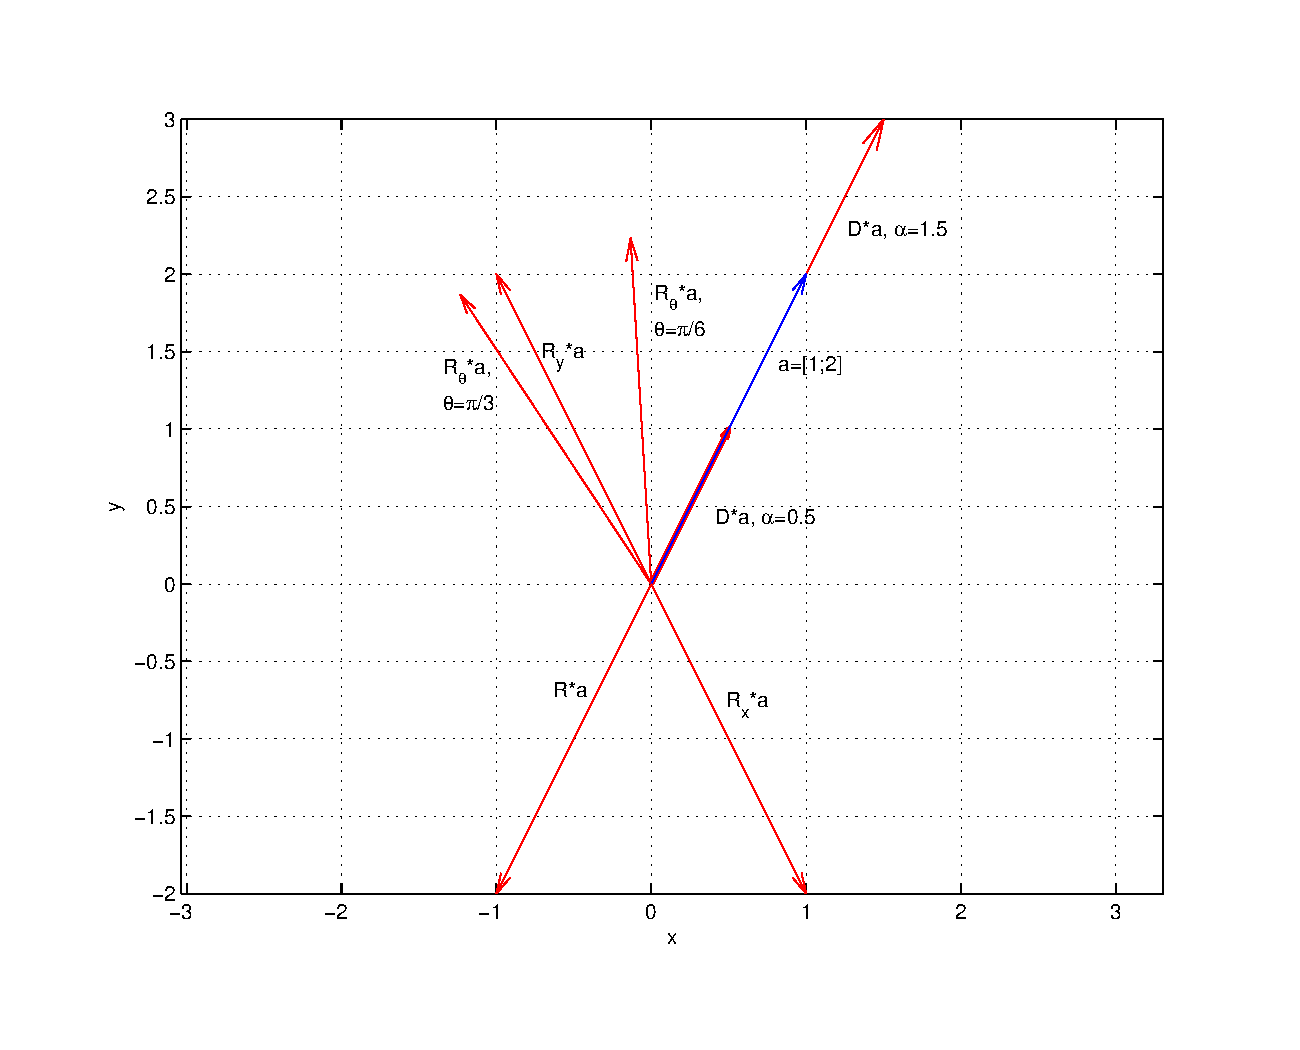
\includegraphics[width=12cm]{ltrans.eps}
\caption{Transformaciones lineales del vector $a=[1;2]$. $D$, dilatación/contracción en un factor $1.5$/$0.5$. $R_x$, reflexión respecto al eje x. $R_y$, reflexión respecto al eje y. $R_{\theta}$ rotaciones respecto al origen para ángulos $\theta=\pi /6$ y $\theta=\pi /3$}
\label{fig:ltrans}
\end{figure}

\begin{paracol}{2}
\paragraph{Norma de una matriz.} La norma de una matriz se puede definir a partir del efecto que produce al actuar, como un operador lineal, sobre un vector. En este caso, se les llama normas \emph{inducidas}. Para una matriz $A$ de orden $m\times n$, $y_{(m)}=A_{(m\times n)}x_{(n)}$, La norma inducida de $A$ se define en función de las normas de los vectores $x$ de su dominio y de las normas de los vectores $y$ de su rango como,
\end{paracol}
\begin{equation*}
\Vert A \Vert =\max_{x \neq 0} \frac{\Vert y \Vert}{\Vert x \Vert}=\max_{x \neq 0} \frac{\Vert Ax \Vert}{\Vert x \Vert}
\end{equation*}

\begin{paracol}{2}
Se puede interpretar como el factor máximo con que el que la matriz $A$ puede \emph{alargar} un vector cualquiera. Es posible definir la norma inducida en función de los vectores unitarios del dominio,
\end{paracol}
\begin{equation*}
\Vert A \Vert =\max_{x \neq 0} \frac{\Vert Ax \Vert}{\Vert x \Vert}= \max_{x \neq 0} \left\Vert A\frac{x}{\Vert x \Vert} \right\Vert= \max_{\Vert x \Vert =1}\Vert Ax \Vert
\end{equation*}

\begin{paracol}{2}
Junto a la norma inducida que acabamos de ver, se definen las siguientes normas,

1. Norma 1: Se suman los elementos de cada columna de la matriz, y se toma como norma el valor máximo de dichas sumas,
\end{paracol}
\begin{equation*}
\Vert A_{m,n} \Vert _{1} = \max_j \sum_{i=1}^m a_{ij}
\end{equation*}
\begin{paracol}{2}
2. Norma $\infty$: Se suman los elementos de cada fila y se toma como norma $\infty$ el valor máximo de dichas sumas.
\end{paracol}
\begin{equation*}
\Vert A_{m,n} \Vert _{\infty} = \max_i \sum_{j=1}^m a_{ij}
\end{equation*}
\begin{paracol}{2}
3. Norma 2: Se define como el mayor de los valores singulares de una matriz. (Ver sección 
\end{paracol}
\ref{sec:SVD}).
\begin{equation*}
\Vert A_{m,n} \Vert _2 = \sigma_{1}
\end{equation*}
\begin{paracol}{2}
4. Norma de Frobenius. Se define como la raíz cuadrada de la suma de los cuadrados de todos los elementos de la matriz,
\end{paracol}
\begin{equation*}
\Vert A_{m,n} \Vert _F =\sqrt{\sum_{i=1}^m \sum_{j=1}^m a_{ij}^2}
\end{equation*}
\begin{paracol}{2}
Que también puede expresarse de forma mas directa como,
\end{paracol}
\begin{equation*}
\Vert A_{m,n} \Vert _F =\sqrt{tr(A^T\cdot A)}
\end{equation*}
\begin{paracol}{2}
En Numpy, es posible calcular las distintas normas de una matriz, de modo análogo a como se calculan para el caso de vectores,  mediante el comando \texttt{norm(A,p)}. Donde \texttt{A}, es ahora un a matriz y \texttt{p} especifica el tipo de norma que se quiere calcular. En el caso de una matriz, el parámetro \texttt{p} solo puede tomar los valores, \texttt{1} (norma 1), \texttt{2} (norma 2), \texttt{inf} (norma $\infty$), y \texttt{'fro'} (norma de frobenius). Esta última es la norma por defecto, y es la que se optiene si se no se define el tipo de normar. El siguiente ejemplo muestra el cálculo de las normas 1, 2, $\infty$ y de Frobenius de la misma matriz.
\end{paracol}
\begin{center}
    \begin{minipage}{0.5\textwidth}
    \begin{minted}{python}
In [11]: A = np.array([[1,-1,3],[2,0,-2],[3,1,2]])

In [12]: A
Out[12]: 
array([[ 1, -1,  3],
       [ 2,  0, -2],
       [ 3,  1,  2]])

In [13]: np.linalg.norm(A)
Out[13]: 5.744562646538029

In [14]: np.linalg.norm(A,'fro')
Out[14]: 5.744562646538029

In [15]: np.linalg.norm(A,1)
Out[15]: 7.0

In [17]: np.linalg.norm(A,inf)
Out[17]: 6.0

In [18]: np.linalg.norm(A,2)
Out[18]: 4.552861506620628
\end{minted}
\end{minipage}
\end{center}

\begin{paracol}{2}
\paragraph{Formas cuadráticas.} Se define como forma cuadrática a la siguiente operación entre una matriz cuadrada $A$ de orden $n \times n$ y un vector $x$ de dimensión $n$,
\end{paracol}
\begin{equation*}
\alpha=x^T\cdot A \cdot x, \ \alpha \in \mathbb{R}
\end{equation*}

\begin{paracol}{2}
El resultado es un escalar. Así por ejemplo,
\end{paracol}

\begin{equation*}
A=\begin{pmatrix}
1& 2& -1\\
2& 0& 2\\
3& 2& -2
\end{pmatrix}, \ x=\begin{pmatrix}
1\\
2\\
3
\end{pmatrix} \rightarrow \begin{pmatrix}
1& 2& 3
\end{pmatrix} \cdot \begin{pmatrix}
1& 2& -1\\
2& 0& 2\\
3& 2& -2
\end{pmatrix} \cdot \begin{pmatrix}
1\\
2\\
3
\end{pmatrix}= 21
\end{equation*}
\begin{paracol}{2}
Para dimensión $n=2$,
\end{paracol}
\begin{equation*}
\alpha =\begin{pmatrix}
x_1& x_2
\end{pmatrix}\cdot \begin{pmatrix}
a_{11}& a_{12}\\
a_{21}& a_{22}
\end{pmatrix}\cdot \begin{pmatrix}
x_1\\
x_2
\end{pmatrix} \rightarrow x_3\equiv \alpha=a_{11}x_1^2+(a_{12}+a_{21})x_1x_2+a_{22}x_2^2
\end{equation*}

\begin{paracol}{2}
Lo que obtenemos, dependiendo de los signos de $a_{11}$ y $a_{12}$, es la ecuación de un paraboloide o un hiperboloide. En la figura \ref{fig:parabol} Se muestra un ejemplo,
\end{paracol}
\begin{figure}[h]
\centering
\includegraphics[width=14cm]{parabol.eps}
\caption{Formas cuadráticas asociadas a las cuatro matrices diagonales: $\vert a_{11}\vert=\vert a_{22}\vert=1$, $a_{12}=a_{21}=0$}
\label{fig:parabol}
\end{figure}
\begin{paracol}{2}
Veamos brevemente, algunas propiedades relacionadas con  las formas cuadráticas,

1. Una matriz $A$ de orden $ n\times n$ se dice que es definida positiva si da lugar a una forma cuadrática que es siempre mayor que cero para cualquier vector no nulo,
\end{paracol}
\begin{equation*}
x^T \cdot A \cdot x > 0, \forall x \neq 0 
\end{equation*}
\begin{paracol}{2}
2. Una matriz \emph{simétrica} es definida positiva si todos sus \emph{valores propios} (ver sección \ref{sec:diag}) son positivos.

3. Una matriz no simétrica $A$ es definida positiva si su parte simétrica $A_s=(A+A^T)/2$ lo es.
\end{paracol}
\begin{equation*}
x\cdot A_s\cdot >0, \forall x \neq 0 \Rightarrow x\cdot A\cdot >0, \forall x \neq 0
\end{equation*}

\begin{flalign*}
&&\reversemathwitch*
\end{flalign*}

\begin{paracol}{2}
\section{Tipos de matrices empleados frecuentemente}\label{tiposm}
Definimos a continuación algunos tipos de matrices frecuentemente empleados en álgebra, algunos ya han sido introducidos en secciones anteriores. Los reunimos todos aquí para facilitar su consulta

1 Matriz ortogonal: Una matriz $A_{n\times n}$ es ortogonal cuando su inversa coincide con su traspuesta.
\end{paracol}
\begin{equation*}
A^T=A^{-1}
\end{equation*}
\begin{paracol}{2}
ejemplo,
\end{paracol}

\begin{equation*}
A=\begin{pmatrix}
1/3& 2/3& 2/3\\
2/3& -2/3& 1/3\\
2/3& 1/3& -2/3\\
\end{pmatrix} \rightarrow A\cdot A^T =A^T\cdot A= \begin{pmatrix}
1& 0& 0\\
0& 1& 0\\
0& 0& 1
\end{pmatrix}
\end{equation*}
\begin{paracol}{2}
2. Matriz simétrica: Una matriz $A_{n\times n}$ es simétrica cuando es igual que su traspuesta,
\end{paracol}
\begin{equation*}
A=A^T \rightarrow a_{ij}=a_{ji}
\end{equation*}
\begin{paracol}{2}
ejemplo,
\end{paracol}
\begin{equation*}
A=\begin{pmatrix}
1& -2& 3\\
-2& 4& 0\\
3& 0& -5
\end{pmatrix}
\end{equation*}
\begin{paracol}{2}
3. Matriz Diagonal: Una matriz $A$  es diagonal si solo son distintos de ceros los elementos de su diagonal principal,
\end{paracol}

\begin{equation*}
\begin{pmatrix}
a_{11}& 0& \cdots & 0\\
0& a_{22}& \cdots & 0\\
\vdots & \vdots & \ddots & 0\\
0& 0& \cdots & a_{nn}
\end{pmatrix} \rightarrow
a_{ij}=0,\ \forall i\neq j
\end{equation*}

\begin{paracol}{2}
4. Matriz triangular superior: Una matriz es triangular superior cuando todos los elementos situados por debajo de la diagonal son cero. Es estrictamente diagonal superior si además los elementos de la diagonal también son cero,
\end{paracol}
\begin{align*}
TRS& \rightarrow a_{ij} = 0, \ \forall i\geq j \\
ETRS& \rightarrow a_{ij} = 0, \ \forall i > j 
\end{align*}
\begin{paracol}{2}
ejemplos,
\end{paracol}

\begin{align*}
TRS&=\begin{pmatrix}
1 & 3 & 7\\
0 & 2 & -1\\
0 & 0 & 4
\end{pmatrix}\\
ETRS&=\begin{pmatrix}
0 & 3 & 7\\
0 & 0 & -1\\
0 & 0 & 0
\end{pmatrix}\\
\end{align*}
\begin{paracol}{2}
5. Matriz triangular inferior: Una matriz es triangular inferior si todos los elementos pro encima de su diagonal son cero. Es estrictamente triangular inferior si además los elementos de su diagonal son también cero,
\end{paracol}
\begin{align*}
TRI& \rightarrow a_{ij} = 0, \ \forall i\leq j \\
ETRI& \rightarrow a_{ij} = 0, \ \forall i < j 
\end{align*}
\begin{paracol}{2}
ejemplos,
\end{paracol}

\begin{align*}
TRI&=\begin{pmatrix}
1 & 0 & 0\\
3 & 2 & 0\\
7 & -1 & 4
\end{pmatrix}\\
ETRI&=\begin{pmatrix}
0 & 0 & 0\\
3 & 0 & 0\\
7 & -1 & 0
\end{pmatrix}\\
\end{align*}
\begin{paracol}{2}
6. Matriz definida Positiva. Una Matriz $A_{n \times n}$ es definida positiva si dado un vector $x$ no nulo cumple,
\end{paracol}
\begin{equation*}
x^T\cdot A \cdot x > 0, \ \forall x\neq 0
\end{equation*}
si,
\begin{equation*}
x^T\cdot A \cdot x \geq 0, \ \forall x\neq 0
\end{equation*}
\begin{paracol}{2}
entonces la matriz $A$ es semidefinida positiva.

7. Una matriz es Diagonal dominante si cada uno de los elementos de la diagonal en valor absoluto es mayor que la suma de los valores absolutos de los elementos de la fila a la  que pertenece.
\end{paracol}

\begin{equation*}
\lvert a_{ii} \rvert > \sum_{j\neq i} \lvert a_{ij} \rvert, \ \forall i
\end{equation*}
\begin{paracol}{2}
ejemplo,
\end{paracol}
\begin{equation*}
A=\begin{pmatrix}
10& 2 & 3\\
2& -5 & 1\\
4& -2 & 8
\end{pmatrix}\rightarrow \left\{ \begin{aligned}
10& > 2+3\\
5&> 2+1\\
8& > 4+2
\end{aligned} \right. 
\end{equation*}

\begin{paracol}{2}
\section{Factorización de matrices}\label{sec:fact}
La factorización de matrices, consiste en la descomposición de una matriz en el producto de dos o más matrices. Las matrices resultantes de la factorización se eligen de modo que simplifiquen, o hagan más robustas numéricamente determinadas operaciones matriciales: Cálculos de determinantes, inversas, etc. A continuación se describen las más comunes.

\subsection{Factorizacion LU}\label{sec:LU}
Consiste en factorizar una matriz como el producto de una matriz triangular inferior $L$ por una  matriz triangular superior $U$, $A=L\cdot U$. Por ejemplo,
\end{paracol}
\begin{equation*}
\begin{pmatrix}
3& 4& 2\\
2& 0& 1\\
3& 2& 1
\end{pmatrix} = \begin{pmatrix}
1& 0& 0\\
^2/_3 & 1& 0\\
1& ^3/_4& 1
\end{pmatrix}\cdot \begin{pmatrix}
3& 4& 2\\
0& ^{-8}/_3& ^{-1}/_3\\
0& 0& ^{-3}/_4
\end{pmatrix}
\end{equation*}
\begin{paracol}{2}
Una aplicación inmediata, es el calculo del determinante. Puesto que el determinante de una matriz triangular, es directamente el producto de los elementos de la diagonal.

En el ejemplo anterior,
\end{paracol}
\begin{equation*}
\vert A \vert = 6 \equiv \vert L \vert\cdot\vert U\vert =1 \cdot 1 \cdot 1 \cdot 3 \cdot (-\frac{8}{3})\cdot (-\frac{3}{4})=6    
\end{equation*}


% Hasta ahora, hemos descrito un procedimiento para transformar una matriz cualquiera en una matriz triangular superior. Nuestro objetivo era obtener la descomposición de un matriz en el producto de dos,  una triangular inferior y otra triangular superior.  En primer lugar, podemos asociar    el procedimiento descrito de eliminación gaussiana al producto de matrices. Volviendo al ejemplo anterior, si construimos la matriz $\lambda_1$
% \begin{equation*}
% \lambda_1=\begin{pmatrix} 
% 1& 0& 0& 0\\
% -2/3& 1& 0& 0\\
% -3/3& 0& 1& 0\\
% -5/3& 0& 0& 1
% \end{pmatrix}
% \end{equation*},
% El producto $\lambda_1 \cdot A$ da como resultado la matriz,

% \begin{equation*} 
%  U_1=\begin{pmatrix}
% 3& 4& 2&5\\
% 0& -2.66& -0.33& -5.33\\
% 0& -2& -1& -3\\
% 0& -4.66& -0.33& -6.33
% \end{pmatrix}=\begin{pmatrix} 
% 1& 0& 0& 0\\
% -2/3& 1& 0& 0\\
% -3/3& 0& 1& 0\\
% -5/3& 0& 0& 1
% \end{pmatrix}\cdot \begin{pmatrix}
% 3& 4& 2&5\\
% 2& 0& 1& -2\\
% 3& 2& 1& 8\\
% 5& 2& 3& 2
% \end{pmatrix}
% \end{equation*}

% De modo análogo, $U_2=\lambda_2 \cdot U_1$
 
% \begin{equation*}
% \lambda_2=\begin{pmatrix} 
% 1& 0& 0& 0\\
% 0& 1& 0& 0\\
% 0& -2/2.66& 1& 0\\
% 0& -4.66/2.66& 0& 1
% \end{pmatrix}
% \end{equation*}

% \begin{equation*}
% U_2= \begin{pmatrix}
% 3& 4& 2&5\\
% 0& -2.6& -0.33& -5.33\\
% 0& 0& -0.75& 7\\
% 0& 0& 0.25& 3
% \end{pmatrix}
% \end{equation*}

% Por último, $U=\lambda_3 \cdot U_2$

% \begin{equation*}
%  \lambda_3 =\begin{pmatrix}
% 1& 0& 0&0\\
% 0& 1& 0& 0\\
% 0& 0& 1& 0\\
% 0& 0& 0.25/0.75 & 1
% \end{pmatrix}
% \end{equation*}

% \begin{equation*}
%  U =\begin{pmatrix}
% 3& 4& 2&5\\
% 0& -2.66& -0.33& -5.33\\
% 0& 0& -0.75& 7\\
% 0& 0& 0& 5.33
% \end{pmatrix}
% \end{equation*}

% De nuevo, podemos generalizar el procedimiento empleado; cada matriz $\lambda_j$ \emph{elimina} todos los elementos de la columna $n$ de una matriz $A$ , situados por debajo de la diagonal. La  matriz $\lambda_j$  toma la forma general,

% \begin{equation*}
% \lambda_j=\begin{pmatrix}
% 1& \cdots & 0& 0& 0& \cdots & 0\\
%  \vdots &  &  \vdots & \vdots &  \vdots & & \vdots\\
% 0& \cdots & 1& 0& 0& \cdots & 0\\
% 0& \cdots & 0& 1& 0& \cdots & 0\\
% 0& \cdots &0 & -a_{j+1,j}/a_{jj}& 0& \cdots & 0\\
% 0& \cdots &0 & -a_{j+2,j}/a_{jj}& 1& \cdots & 0\\
%  \vdots &  &  \vdots & \vdots &  \vdots & & \vdots\\
% 0& \cdots & 0& -a_{n,j}/a_{jj}& 0&\cdots & 1\\
% \end{pmatrix}
% \end{equation*} 
% Solo los elementos de la diagonal, que toman el valor $1$, y los elementos de la columna $j$ situados por debajo de la diagonal son distintos de cero.

% A partir de la definición de las matrices $\lambda_j$, podemos obtener una relación entre la matriz triangular superior $U$  obtenida al final del proceso de eliminación, y la matriz inicial $A$ de orden $n\times n$ para ello, en cada paso multiplicamos tanto por $\lambda_j$ como por su inversa $\lambda_j^{-1}$,
% \begin{align*}
% A&=\lambda_1^{-1}\cdot \overbrace{\lambda_1\cdot A}^{U_1}\\
% A&=\lambda_1^{-1}\cdot\lambda_2^{-1} \cdot \overbrace{\lambda_2  \cdot \lambda_1 A}^{U_2}\\
% A&=\lambda_1^{-1}\cdot \lambda_2^{-1}\cdot \overbrace{ \lambda_3^{-1}\cdot  \lambda_3 \cdot  \lambda_2\cdot \lambda_1 \cdot A}^{U_3}\\
% \vdots \\
% A&=\lambda_1^{-1} \cdot  \lambda_2^{-1}\cdot  \lambda_3^{-1} \cdots  \lambda_n ^{-1}\cdot \overbrace{\lambda_n \cdots \lambda_3 \cdot \lambda_2\cdot \lambda_1  \cdot A}^{U}
% \end{align*}

% Las matrices $\lambda_j^{-1}$ tienen dos propiedades que las hacen particularmente fáciles de manejar:  la primera es que cumplen que  su inversa  $\lambda_j^{-1}$ puede obtenerse a partir de $\lambda_j$, sin más que cambiar de signo los elementos distintos de cero que no pertenecen a la diagonal (Compruébalo),
% \begin{equation*}
%  \lambda_j^{-1}=\begin{pmatrix}
% 1& \cdots & 0& 0& 0& \cdots & 0\\
%  \vdots &  &  \vdots & \vdots &  \vdots & & \vdots\\
% 0& \cdots & 1& 0& 0& \cdots & 0\\
% 0& \cdots & 0& 1& 0& \cdots & 0\\
% 0& \cdots &0 & a_{j+1j}/a_{jj}& 0& \cdots & 0\\
% 0& \cdots &0 & a_{j+2j}/a_{jj}& 1& \cdots & 0\\
%  \vdots &  &  \vdots & \vdots &  \vdots & & \vdots\\
% 0& \cdots & 0& a_{nj}/a_{jj}& 0&\cdots & 1\\
% \end{pmatrix}
% \end{equation*}

% La segunda propiedad es que el producto $L=\lambda_1^{-1} \cdot  \lambda_2^{-1}\cdot  \lambda_3^{-1} \cdots  \lambda_n ^{-1}$, se puede obtener progresivamente, a la vez que se construye $U$, sin más que ir juntando en una única matriz $L$ las columnas de $\lambda_1^{-1}$, $\lambda_2^{-1}$, etc. que contienen elementos no nulos, en nuestro ejemplo,
% \begin{equation*}
%  L =\begin{pmatrix}
% 1& 0& 0&0\\
% 2/3& 1& 0& 0\\
% 3/3& 2/2.66& 1& 0\\
% 5/3& 4.66/2.66& -0.25/0.75 & 1
% \end{pmatrix}
% \end{equation*}

% y, en general,

% \begin{equation*}
%  L=\begin{pmatrix}
% 1& \cdots & 0& 0& 0& \cdots & 0\\
%  \vdots &  &  \vdots & \vdots &  \vdots & & \vdots\\
% a_{j-11}/a_{11}& \cdots & 1& 0& 0& \cdots & 0\\
% a_{j1}/a_{11}& \cdots & a_{jj-1}/a_{j-1 j-1}& 1& 0& \cdots & 0\\
% a_{j+11}/a_{11}& \cdots &a_{j+1j-1}/a_{j-1 j-1} & a_{j+1j}/a_{jj}& 0& \cdots & 0\\
% a_{j+11}/a_{11}& \cdots &a_{j+2j-1}/a_{j-1 j-1} & a_{j+2j}/a_{jj}& 1& \cdots & 0\\
%  \vdots &  &  \vdots & \vdots &  \vdots & & \vdots\\
% a_{n1}/a_{11}& \cdots & a_{nj-1}/a_{j-1j-1}& a_{nj}/a_{jj}& a_{nj+1}/a_{j+1j+1}&\cdots & 1\\
% \end{pmatrix}
% \end{equation*}

% Por construcción,  la matriz $L$ es una matriz inferior, Con lo que quedaría completo el cálculo de la factorización LU,

% \begin{equation*}
% A=\overbrace{\lambda_1^{-1} \cdot  \lambda_2^{-1}\cdot  \lambda_3^{-1} \cdots  \lambda_n ^{-1}}^{L}\cdot \overbrace{\lambda_n \cdots \lambda_3 \cdot \lambda_2\cdot \lambda_1  \cdot A}^{U}=L\cdot U
% \end{equation*}

% La factorización que acabamos de describir, puede presentar problemas numéricos dependiendo del cómo sea la matriz que se desea factorizar. El primer problema se produce cuando el elemento de la diagonal de $u_{jj}$ por el que toca dividir para eliminar los elementos de la columna $j$, situados por debajo de la diagonal, es $0$. En ese caso el ordenador dará un error de desbordamiento y no se podrá seguir factorizando. El segundo problema surge cuando los elementos de la matriz son dispares en magnitud; las operaciones matemáticas realizadas durante el proceso de factorización pueden dar lugar a errores de redondeo importantes que hagan incorrecto el resultado de la factorización. Veamos un ejemplo un tanto extremo,

% \begin{equation*}
% \begin{pmatrix}
% 10^{-20}& 1\\
% 1& 1 
% \end{pmatrix}=\overbrace{\begin{pmatrix}
% 1& 0\\
% 10^{20}& 1 
% \end{pmatrix}}^{L}\cdot \overbrace{\begin{pmatrix}
% 1& 0\\
% -10^{20}& 1
% \end{pmatrix}\cdot \begin{pmatrix}
% 10^{-20}& 1\\
% 1& 1
% \end{pmatrix}}^{U}= \overbrace{\begin{pmatrix}
% 1& 0\\
% 10^{20}& 1 
% \end{pmatrix}}^{L} \cdot \overbrace{\begin{pmatrix}
% 10^{-20}& 1\\
% 0& 1 -10^{20} 
% \end{pmatrix}}^{U} 
% \end{equation*} 

% Como el \emph{eps} del ordenador es del orden de $10^{-16}$, $1$ es despreciado frente $10^{20}$. Es decir, $(1-10^{20})\approx 10^{20}$, con lo cual el ordenador tendrá una versión aproximada de $U$

% \begin{equation*}
% U \approx \hat{U}= \begin{pmatrix}
% 10^{-20}& 1\\
% 0& -10^{20} 
% \end{pmatrix} 
% \end{equation*}

% Pero si ahora volvemos a multiplicar $L\cdot U$  para recuperar $A$,
% \begin{equation*}
% L \cdot \hat{U}=  \begin{pmatrix}
% 1& 0\\
% 10^{20}& 1 
% \end{pmatrix} \cdot \begin{pmatrix}
% 10^{-20}& 1\\
% 0& -10^{20} 
% \end{pmatrix}= \begin{pmatrix}
% 10^{-20}& 1\\
% 1& 0
% \end{pmatrix} \neq A
% \end{equation*}

% Una manera de paliar los efectos de redondeo, es reordenar las filas de la matriz de modo que el elemento $a_{jj}$ por el que se va a dividir los elementos de la fila $j$ en el proceso de eliminación sea lo mayor posible. Este procedimiento se conoce con el nombre de pivoteo de filas.
% Para el ejemplo que acabamos de examinar, supongamos que cambiamos de orden las dos filas de    la matriz,

% \begin{equation*}
% \begin{pmatrix}
% 10^{-20}& 1\\
% 1& 1 
% \end{pmatrix} \rightarrow \begin{pmatrix}
% 1& 1\\
% 10^{-20}& 1 
% \end{pmatrix}
% \end{equation*}

% Si recalculamos la factorización LU, para la nueva matriz con la filas intercambiadas,

% \begin{equation*}
% \begin{pmatrix}
% 1& 1\\
% 10^{-20}& 1 
% \end{pmatrix}=\overbrace{\begin{pmatrix}
% 1& 0\\
% 10^{-20}& 1 
% \end{pmatrix}}^{L}\cdot \overbrace{\begin{pmatrix}
% 1& 0\\
% -10^{-20}& 1
% \end{pmatrix}\cdot \begin{pmatrix}
% 1& 1\\
% 10^{-20}& 1 
% \end{pmatrix}}^{U}= \overbrace{\begin{pmatrix}
% 1& 0\\
% 10^{-20}& 1 
% \end{pmatrix}}^{L} \cdot \overbrace{\begin{pmatrix}
% 1& 1\\
% 0&  1-10^{-20}
% \end{pmatrix}}^{U} 
% \end{equation*}

% De nuevo, por errores de redondeo el ordenador tendrá una version aproximada de $U$.

% \begin{equation*}
% U \approx \hat{U}= \begin{pmatrix}
% 1& 1\\
% 0& 1 
% \end{pmatrix} 
% \end{equation*}

% Sin embargo si recalculamos el producto $L\cdot \hat{U}$ y volvemos a reordenar las filas del resultado,
% \begin{equation*}
% L \cdot \hat{U}=  \begin{pmatrix}
% 1& 0\\
% 10^{-20}& 1 
% \end{pmatrix} \cdot \begin{pmatrix}
% 1& 1\\
% 0& 1 
% \end{pmatrix}= \begin{pmatrix}
% 1& 1\\
% 10^{-20}& 1+10^{-20}
% \end{pmatrix} \rightarrow \begin{pmatrix}
% 10^{-20}& 1+10^{-20}\\
% 1& 1
% \end{pmatrix} \approx A
% \end{equation*}
\begin{paracol}{2}
Describir un método para realizar la factorización LU de una matriz, queda fuera de los objetivos de estos apuntes. Sin embargo sí que utilizaremos el comando \mintinline{python}{lu} incluido en una librería de Python llamada Scipy para obtener directamente el resultado de una factorización LU. Es una librería parecida a Numpy y que, al igual que esta última contiene un gran numero de funciones matemáticas. De hecho Numpy y Scipy solapan un poco y hay determinadas funciones que pueden encontrarse en ambas librerías. El comando pertenece a un submodulo de Scipy llamado \mintinline{python}{linalg}. Admite como variable de entrada una matriz cuadrada $A$ y nos devuelve como salida una matriz de permutación $P$, de la que hablaremos enseguida, y una matriz triangular inferior $L$ y otra triangular superior $U$ de modo que se cumple que $A =PLU$,

A veces obtener la factorización LU directa de una matriz, pude llevar a cálculos que son numéricamente inestables afectando a la precisión del resultado. Una manera de paliar este efecto es permutar entre sí algunas de las filas de la matriz que se quiere factorizar y factorizar la versión permutada.

La permutación de las filas de una matriz $A$ de orden $n\times m$, se puede definir a partir del producto con las matrices de permutación de orden $n \times n$. Éstas se obtienen permutando directamente las filas de la matriz identidad $I_{n \times n}$. Si una matriz de permutación multiplica a otra matriz por la izquierda, permuta el orden de sus filas. Si la multiplica por la derecha. permuta el orden de sus columnas. Así por ejemplo, para matrices de orden $3 \times n$,
\end{paracol}
\begin{equation*}
I_{n \times n}=\begin{pmatrix}
1& 0& 0\\
0& 1& 0\\
0& 0& 1\\
\end{pmatrix} \rightarrow P_{1 \leftrightarrow 3}= \begin{pmatrix}
0& 0& 1\\
0& 1& 0\\
1& 0& 0\\
\end{pmatrix}
\end{equation*}
\begin{paracol}{2}
Si multiplicamos $P_{1 \leftrightarrow 3}$ con cualquier otra matriz $A$ de orden $3\times n$, El resultado es equivalente a intercambiar en la matriz $A$ la fila $1$ con la $3$. Por ejemplo,
\end{paracol}
\begin{equation*}
P_{1\leftrightarrow 3}\cdot A=\begin{pmatrix}
0& 0& 1\\
0& 1& 0\\
1& 0& 0\\
\end{pmatrix} \cdot \begin{pmatrix}
1& 2& 5& 3\\
4& 2& 3& 0\\
3& 6& 2& 1
\end{pmatrix} = \begin{pmatrix}
3& 6& 2& 1\\
4& 2& 3& 0\\
1& 2& 5& 3
\end{pmatrix}= A_{1\leftrightarrow 3}
\end{equation*}

% Volvamos al cálculo de la factorización LU, pero ahora empleando la permutación de filas. Supongamos una matriz $A$ de orden $n\times n$

% El primer paso, es buscar el elemento mayor en valor absoluto de la primera columna en intercambia la primera fila de la matriz de $A$, con la fila que contiene dicho elemento. Si utilizamos la matriz de permutación adecuada, esto puede expresarse como,

% \begin{equation*}
% A \rightarrow P_1\cdot A
% \end{equation*}
% A continuación eliminamos los elementos de la primera fila situados por debajo de la diagonal,
% \begin{equation*}
% A \rightarrow P_1\cdot A \rightarrow \lambda_1 \cdot P_1 \cdot A
% \end{equation*}
% Volvemos a buscar el mayor elemento en valor absoluto para la segunda columna (Solo desde la diagonal hasta el ultimo elemento de la columna).  
% \begin{equation*}
% A \rightarrow P_1\cdot A \rightarrow \lambda_1 \cdot P_1 \cdot A \rightarrow  P_2 \cdot \lambda_1 \cdot P_1 \cdot A 
% \end{equation*}

% Eliminamos los elementos de la segunda fila situados por debajo de la diagonal,

% \begin{equation*}
% A \rightarrow P_1\cdot A \rightarrow \lambda_1 \cdot P_1 \cdot A \rightarrow  P_2 \cdot \lambda_1 \cdot P_1 \cdot A \rightarrow \lambda_2 \cdot  P_2 \cdot \lambda_1 \cdot P_1 \cdot A
% \end{equation*}

% Si seguimos todo el proceso hasta eliminar los elementos situados por debajo de la diagonal en la fila $n-1$, obtendremos la expresión de la matriz triangular superior $U$ resultante,

% \begin{equation*}
% \lambda_{n-1}P_{n-1}\lambda_{n-2}P_{n-2} \cdots  \lambda_2  P_2 \lambda_1  P_1 A = U
% \end{equation*}

% Aunque hemos obtenido $U$, necesitamos una manera de obtener $L$, ahora no es inmediato como en el caso de la factorización sin pivoteo, no basta con invertir las matrices $\lambda_i$ ya que tenemos por medio todas las matrices de permutación utilizadas. Para obtenerla realizaremos la siguiente transformación, 

% \begin{equation*}
% \lambda_{n-1}P_{n-1}\lambda_{n-2}P_{n-2} \cdots  \lambda_2  P_2 \lambda_1  P_1 A = \lambda_{n-1}'\lambda_{n-2}'\cdots \lambda_2'   \lambda_1' P_{n-1}P_{n-2} \cdots P_2  P_1 A
% \end{equation*}

% Donde las matrices $\lambda_i'$ pueden obtenerse a partir de las matrices $\lambda_i$ y de las matrices de permutación de la manera siguiente,

% \begin{align*}
% \lambda_{n-1}' &= \lambda_{n-1} \\
% \lambda_{n-2}' &= P_{n-1}\lambda_{n-2} P_{n-1} ^{-1}\\
% \lambda_{n-3}' &= P_{n-1}P_{n-2}\lambda_{n-3}P_{n-2}^{-1} P_{n-1}^{-1} \\
%  & \vdots \\
%  \lambda_{k\ \ }'  &= P_{n-1}P_{n-2}\cdots P_{k+1} \lambda_{k}P_{k+1}^{-1} \cdots P_{n-2}^{1} P_{n-1}^{-1} \\
%  & \vdots \\
% \lambda_{2\ \ }'  &= P_{n-1}P_{n-2}\cdots P_3 \lambda_{2}P_3^{-1} \cdots P_{n-2}^{1} P_{n-1}^{-1} \\
% \lambda_{1\ \ }'  &= P_{n-1}P_{n-2}\cdots P_3P_2 \lambda_{1}P_2^{-1}P_3^{-1} \cdots P_{n-2}^{1} P_{n-1}^{-1} \\
% \end{align*}


% Matemáticamente el cálculo de las matrices $\lambda_i'$ requiere calcular el producto de un gran número de matrices.  Sin embargo dicho cálculo es equivalente a permutar los elementos de $\lambda_i$ situados por debajo de la diagonal.   Así Por ejemplo para,

% \begin{equation*}
% \lambda_2=
% \begin{pmatrix}
% 1& 0& 0& 0\\
% 0& 1& 0& 0\\
% 0& 2& 1& 0\\
% 0& 3& 0& 1
% \end{pmatrix}, \ 
% P_3=
% \begin{pmatrix}
% 1& 0& 0& 0\\
% 0& 1& 0& 0\\
% 0& 0& 0& 1\\
% 0& 0& 1& 0
% \end{pmatrix}
% \end{equation*}

% \begin{equation*}
% \lambda_2'=P_3\cdot \lambda_2 P_3^{-1}
% \begin{pmatrix}
% 1& 0& 0& 0\\
% 0& 1& 0& 0\\
% 0& 0& 0& 1\\
% 0& 0& 1& 0
% \end{pmatrix}\cdot \begin{pmatrix}
% 1& 0& 0& 0\\
% 0& 1& 0& 0\\
% 0& 2& 1& 0\\
% 0& 3& 0& 1
% \end{pmatrix} \cdot \begin{pmatrix}
% 1& 0& 0& 0\\
% 0& 1& 0& 0\\
% 0& 0& 0& 1\\
% 0& 0& 1& 0
% \end{pmatrix} = \begin{pmatrix}
% 1& 0& 0& 0\\
% 0& 1& 0& 0\\
% 0& 3& 1& 0\\
% 0& 2& 0& 1
% \end{pmatrix}
% \end{equation*}

% Por último podemos representar el producto de todas las matrices de permutación como una sola matriz, $P_{n-1}P_{n-2} \cdots P_2  P_1=P$. (El producto de matrices de permutación entre sí, da como resultado una nueva matriz de permutación.

 
% De esta manera, la factorización LU con pivoteo de filas podríamos representarla como $P\cdot A=L\cdot U$,

% \begin{equation*}
% \overbrace{P_{n-1}P_{n-2} \cdots P_2  P_1}^{P}\cdot  A= \overbrace{\lambda_1'^{-1} \lambda_2'^{-2} \cdots \lambda_{n-2}'^{-1} \lambda_{n-1}'^{-1}}^{L}\cdot \overbrace{\lambda_{n-1}P_{n-1}\lambda_{n-2}P_{n-2} \cdots  \lambda_2  P_2 \lambda_1  P_1 A }^{U}   
% \end{equation*}
\begin{paracol}{2}
Como ejemplo, vamos a calcular la factorización LU de la matriz,
\end{paracol}
\begin{equation*}
A=\begin{pmatrix}
3& 4& 2&5\\
2& 0& 1& -2\\
3& 2& 1& 8\\
5& 2& 3& 2
\end{pmatrix} 
\end{equation*}
%  Pero empleando ahora pivoteo de filas.
 
% En primer lugar buscamos  el elemento de la primera columna mayor en valor absoluto. En esta caso es el último elemento de la columna por lo que intercambiamos la primera fila con la cuarta,
 
 
%   \begin{equation*}
% P_1\cdot A=\begin{pmatrix}
% 0& 0& 0& 1\\
% 0& 1& 0& 0\\
% 0& 0&1& 0\\
% 1& 0& 0& 0
% \end{pmatrix}\begin{pmatrix}
% 3& 4& 2&5\\
% 2& 0& 1& -2\\
% 3& 2& 1& 8\\
% 5& 2& 3& 2
% \end{pmatrix}= \begin{pmatrix}
% 5& 2& 3& 2\\
% 2& 0& 1& -2\\
% 3& 2& 1& 8\\
% 3& 4& 2&5
% \end{pmatrix}
% \end{equation*}

% Eliminamos ahora los elementos de la primera columna situados por debajo de la diagonal,

% \begin{equation*}
% \overbrace{\lambda_1 \cdot P_1\cdot A}^{U_1}=\begin{pmatrix}
% 1& 0& 0& 0\\
% -2/5& 1& 0& 0\\
% -3/5& 0& 1& 0\\
% -3/5& 0& 0&1
% \end{pmatrix} \cdot \begin{pmatrix}
% 5& 2& 3& 2\\
% 2& 0& 1& -2\\
% 3& 2& 1& 8\\
% 3& 4& 0&5
% \end{pmatrix}= \begin{pmatrix}
% 5& 2& 3& 2\\
% 0& -0.8& -0.2& -2.8\\
% 0& 0.8& -0.8& -6.8\\
% 0& 2.8& 0.2&3.8
% \end{pmatrix}
% \end{equation*}

% Para eliminar los elementos de la segunda columna, repetimos los mismos pasos. El elemento mayor de la segunda columna de $U_1$ es ahora $2.8$, por tanto intercambiamos entre sí la segunda y la cuarta fila,

% \begin{equation*}
% P_2\cdot \overbrace{\lambda_1 \cdot P_1\cdot A}^{U_1}=\begin{pmatrix}
% 1& 0& 0& 0\\
% 0& 0& 0& 1\\
% 0& 0& 1& 0\\
% 0& 1& 0&0
% \end{pmatrix} \cdot \begin{pmatrix}
% 5& 2& 3& 2\\
% 0& -0.8& -0.2& -2.8\\
% 0& 0.8& -0.8& -6.8\\
% 0& 2.8& 0.2&3.8
% \end{pmatrix}= \begin{pmatrix}
% 5& 2& 3& 2\\
% 0& 2.8& 0.2&3.8\\
% 0& 0.8& -0.8& -6.8\\
% 0& -0.8& -0.2& -2.8
% \end{pmatrix}
% \end{equation*}
% A continuación, eliminamos los elementos de la segunda columna situados por debajo de la diagonal,

% \begin{equation*}
% \overbrace{\lambda_2\cdot P_2\cdot \lambda_1 \cdot P_1\cdot A}^{U_2}=\begin{pmatrix}
% 1& 0& 0& 0\\
% 0& 1& 0& 0\\
% 0& -0.8/2.8& 1& 0\\
% 0& 0.8/2.8& 0&1
% \end{pmatrix} \cdot \begin{pmatrix}
% 5& 2& 3& 2\\
% 0& 2.8& 0.2&3.8\\
% 0& 0.8& -0.8& -6.8\\
% 0& -0.8& -0.2& -2.8
% \end{pmatrix} = \begin{pmatrix}
% 5& 2& 3& 2\\
% 0& 2.8& 0.2&3.8\\
% 0& 0& -0.85& -5.71\\
% 0& 0& -0.14& -1.71
% \end{pmatrix}
% \end{equation*}

% Para eliminar el elemento que queda debajo de la diagonal en la tercera columna, procedemos igual que para las columnas anteriores. Como en este caso, el elemento situado en la diagonal es mayor en valor absoluto no es preciso permutar. (Desde un punto de vista formal, podríamos decir que en este caso la matriz de permutaciones aplicada es la matriz identidad).

% \begin{align*}
% \overbrace{\lambda_3\cdot\lambda_2\cdot P_2\cdot \lambda_1 \cdot P_1\cdot A}^{U}&=\begin{pmatrix}
% 1& 0& 0& 0\\
% 0& 1& 0& 0\\
% 0& 0& 1& 0\\
% 0& 0& -0.14/0.85&1
% \end{pmatrix} \cdot \begin{pmatrix}
% 5& 2& 3& 2\\
% 0& 2.8& 0.2&3.8\\
% 0& 0& -0.85& -5.71\\
% 0& 0& -0.14& -1.71
% \end{pmatrix}\\ 
% &= \begin{pmatrix}
% 5& 2& 3& 2\\
% 0& 2.8& 0.2&3.8\\
% 0& 0& -0.85& -5.71\\
% 0& 0& 0& -2.66
% \end{pmatrix}= U 
% \end{align*}

% Como hemos visto, la matriz $\lambda_i'$ las obtenemos a  partir de $\lambda_i$, permutando los elementos situados por debajo de la diagonal, distintos de cero. En nuestro ejemplo solo hay matriz $\lambda_1$ afectada por una única permutación $P_2$,
% \begin{equation*}
% \lambda'_1=\begin{pmatrix}
% 1& 0& 0& 0\\
% 3/5& 1& 0& 0\\
% 3/5& 0& 1& 0\\
% 2/5& 0& 0& 1
% \end{pmatrix}
% \end{equation*}

% Para el resto, $\lambda_2'=\lambda_2$ y $\lambda'_3=\lambda_3$. Para obtener la matriz L cambiando los signos a los elementos situados por debajo de la diagonal de $\lambda'_1$, $\lambda_2$ y $\lambda_3$, y los agrupamos en una única matriz,

% \begin{equation*}
% L=\begin{pmatrix}
% 1& 0& 0& 0\\
% 3/5& 1& 0& 0\\
% 3/5& 0.8/2.8& 1& 0\\
% 2/5& -0.8/2.8& 0.14/0.85& 1
% \end{pmatrix}
% \end{equation*}

% Por último debemos multiplicar las matrices de permutaciones para agruparlas en una sola,

% \begin{equation*}
% P=P_2\cdot P_1= \begin{pmatrix}
% 0& 0& 0& 1\\
% 1& 0& 0& 0\\
% 0& 0& 1& 0\\
% 0& 1& 0& 0
% \end{pmatrix}
% \end{equation*}

% Es trivial comprobar que las matrices obtenidas cumplen \footnote{Los valores numéricos empleados en el texto, están redondeados, por tanto dan una solución incorrecta. Si se reproducen las operaciones descritas en Matlab el resultado es mucho más preciso.} $P\cdot A = L\cdot U$.

% El siguiente código calcula la factorización LU de una matriz de orden arbitrario con pivoteo de filas. \label{lufact} 

% \begin{lstlisting}
% function [L,U,P]=lufact(A)
% % este programa calcula una factorizacionLU, de la matrix A,  empleando 
% % el método de eliminacion gaussiana con pivoteo de filas...
% % L es una matriz triangular inferior, U es una matriz triangular superior y
% % P es una matriz de permutaciones tal que P*A=L*U

% % vamos a aprovechar la potencia de Matlab para evitar algunos buques en
% % los calculos..

% % primero definimos la matriz de permutaciones como la matriz identidad de
% % orden igual al número de filas de la matriz A, (si no hay pivoteo de filas 
% % la matriz de permutaciones es precisamente la identidad)

% t=size(A,1); % obtenemos el numero de filas de la matriz A
% P=eye(t); % Construimos la matriz identidad 
% % Ademas, inicializamos las matrices L y U
% L=P;
% U=A;


% % iniciamos un bucle para ir recorriendo las columnas (solo tenemos que
% % recorrer tantas columnas como fila - 1 tenga la matriz A
% for j=1:t-1
%     LA=zeros(t); %Matriz auxiliar (Lambda) de cada iteración.
%     % Buscamos el elemento mas grande de la columna j
%     maxcol=abs(U(j,j)); 
%     index=j;
%     for i=j:t
%         if abs(U(i,j))>maxcol
%             maxcol=abs(U(i,j));
%             index=i;
%         end
%     end
    
%     % reordenamos las filas de P, L y U de modo que el valor mas grande de
%     % j pase a acupar la diagonal (Esto es equivalente a multiplicar U por
%     % la matriz de permetuciones correspondiente, ir calculado
%     % iterativamente el valor de la matriz de permutaciones P final, y
%     % reordenar las filas ya calculadas de L (aportadas por los valores de
%     % las matrices lambdas anteriores... a lambda_j)
    
%     Aux=U(j,:);
%     Aux2=P(j,:);
%     Aux3=L(j,1:j-1);
    
%     % Reordenamos U (Toda la fila)
%     U(j,:)=U(index,:);
%     U(index,:)=Aux;
    
%     % Reordenamos L (Solo los elementos de la columnas anteriores...situados
%     % por debajo de la diagonal).
%     L(j,1:j-1)=L(index,1:j-1);
%     L(index,1:j-1)=Aux3;
    
%     % modificamos la matriz de permutaciones
%     P(j,:)=P(index,:);
%     P(index,:)=Aux2;
    
%    % Calculamos una matriz auxiliar con los factores de los elementos
%    % a eliminar. 
%    LA(j+1:t,j)=U(j+1:t,j)/U(j,j); % estos elementos son directamente los que 
%    % se añaden a la matriz L
%    % Modificamos L y U
%    L(j+1:t,j)=U(j+1:t,j)/U(j,j);
%    U=(eye(t)-LA)*U; % la expresión eye(t)-LA nos permite cambiar de signo los
%    % elementos situados por debajo de la diagonal principal...
% end
% \end{lstlisting}


% Desde el punto de vista de la implementación, el código anterior simplifica el cálculo de la factorización LU,

% \begin{enumerate}
% \item  no se calculan la inversa de $\lambda_i$. En realidad lo que se hace es ir construyendo iterativamente la matriz L: en cada iteración, primero se permutan los elementos de las columnas de la matriz L construida en la iteración anterior, y se añaden los elementos de la columna correspondiente.
% \item la matriz de permutación se va calculando también iterativamente, intercambiando las filas de la matriz de permutación obtenida en la iteración anterior.
% \end{enumerate}
\begin{paracol}{2}
 Scipy, calcula siempre la factorización LU, permutando las filas para obtener un resultado lo mas preciso posible,
\end{paracol}
\begin{center}
\begin{minipage}{0.7\textwidth}
\begin{minted}{python}
In [213]: A = np.array([[3,4,2,5],[2,0,1,-2],[3,2,1,8],[5,2,3,2]])

In [214]: A
Out[214]: 
array([[ 3,  4,  2,  5],
       [ 2,  0,  1, -2],
       [ 3,  2,  1,  8],
       [ 5,  2,  3,  2]])

In [215]: import scipy as sp

In [216]: [P,L,U] = sp.linalg.lu(A)

In [217]: P
Out[217]: 
array([[0., 1., 0., 0.],
       [0., 0., 0., 1.],
       [0., 0., 1., 0.],
       [1., 0., 0., 0.]])

In [218]: L
Out[218]: 
array([[ 1.        ,  0.        ,  0.        ,  0.        ],
       [ 0.6       ,  1.        ,  0.        ,  0.        ],
       [ 0.6       ,  0.28571429,  1.        ,  0.        ],
       [ 0.4       , -0.28571429,  0.16666667,  1.        ]])

In [219]: U
Out[219]: 
array([[ 5.        ,  2.        ,  3.        ,  2.        ],
       [ 0.        ,  2.8       ,  0.2       ,  3.8       ],
       [ 0.        ,  0.        , -0.85714286,  5.71428571],
       [ 0.        ,  0.        ,  0.        , -2.66666667]])

In [220]: P @ L @ U
Out[220]: 
array([[ 3.,  4.,  2.,  5.],
       [ 2.,  0.,  1., -2.],
       [ 3.,  2.,  1.,  8.],
       [ 5.,  2.,  3.,  2.]])
\end{minted}
\end{minipage}
\end{center}

\begin{paracol}{2}
\subsection{Factorización de Cholesky}\label{chol}
Dada una matriz cuadrada, simétrica y definida positiva, es siempre posible factorizarla como $A=L\cdot L^T$. Donde $L$ es una matriz triangular inferior,
\end{paracol}
\begin{equation*}
\begin{pmatrix}
a_{11}& a_{12}& \cdots & a_{1n}\\
a_{12}& a_{22}& \cdots & a_{2n}\\
\vdots & \vdots & \ddots & \vdots\\
a_{1n}& a_{2n}& \cdots & a_{nn}
\end{pmatrix}=\begin{pmatrix}
L_{11}& 0& \cdots & 0\\
L_{21}& L_{22}& \cdots & 0\\
\vdots & \vdots & \ddots & \vdots\\
L_{n1}& L_{n2}& \cdots & L_{nn}
\end{pmatrix} \cdot \begin{pmatrix}
L_{11}& L_{21}& \cdots & L_{n1}\\
0& L_{22}& \cdots & L_{n2}\\
\vdots & \vdots & \ddots & \vdots\\
0& 0& \cdots & L_{nn}
\end{pmatrix}
\end{equation*}
\begin{paracol}{2}
Numpy tiene una función, en el submódulo \mintinline{python}{linalg}, llamada \mintinline{python}{cholesky}, que permite obtener la factorización de Cholesky, 
\end{paracol}
\begin{center}
    \begin{minipage}{0.5\textwidth}
    \begin{minted}{python}
In [224]: B
Out[224]: 
array([[47, 28, 26, 45],
       [28, 24, 16, 40],
       [26, 16, 15, 22],
       [45, 40, 22, 97]])

In [225]: L = np.linalg.cholesky(B)

In [226]: L
Out[226]: 
array([[ 6.8556546 ,  0.        ,  0.        ,  0.        ],
       [ 4.08421976,  2.70539257,  0.        ,  0.        ],
       [ 3.79248978,  0.18874832,  0.76249285,  0.        ],
       [ 6.56392462,  4.87599823, -5.00195311,  2.2627417 ]])

In [227]: L @ L.T
Out[227]: 
array([[47., 28., 26., 45.],
       [28., 24., 16., 40.],
       [26., 16., 15., 22.],
       [45., 40., 22., 97.]])
    \end{minted}
        
    \end{minipage}
\end{center}

\begin{paracol}{2}
Si la matriz no es definida positiva, la función \mintinline{python}{cholesky} da un mensaje de error.

\subsection{Diagonalización}\label{sec:diag}
\paragraph{Autovectores y autovalores.} Dada una matriz $A$ de orden $n\times n$, se define como autovector, o vector propio de dicha matriz al vector $x$ que cumple,
\end{paracol}
\begin{equation*}
A\cdot x =\lambda \cdot x, \  x\neq 0, \ \lambda \in \mathbb{C}
\end{equation*}
\begin{paracol}{2}
Es decir, el efecto de multiplicar la matriz $A$ por el vector $x$ es equivalente a multiplicar el vector $x$  por un número $\lambda$ que, en general, será un número complejo.

$\lambda$ recibe el nombre de autovalor, o valor propio de la matriz $A$. Así por ejemplo,
\end{paracol}
\begin{equation*}
A= \begin{pmatrix}
-2& 0& 0\\
0& 2 & -1\\
0& 0& 3
\end{pmatrix}
\end{equation*}

\begin{paracol}{2}
tiene un autovalor $\lambda=3$ para el vector propio, $x=[0,\  -3,\  3]^T$ ,
\end{paracol}

\begin{equation*}
\begin{pmatrix}
-2& 0& 0\\
0& 2 & -1\\
0& 0& 3
\end{pmatrix}\cdot \begin{pmatrix}
0\\
-3\\
3
\end{pmatrix}=3\cdot \begin{pmatrix}
0\\
-3\\
3
\end{pmatrix}=\begin{pmatrix}
0\\
-9\\
9
\end{pmatrix}
\end{equation*}
\begin{paracol}{2}
El vector propio asociado a un valor propio no es único, si $x$ es un vector propio de una matriz $A$, asociado a un valor propio $\lambda$, Es trivial comprobar que cualquier vector de la forma $\alpha\cdot x, \ \alpha \in \mathbb{C}$ también es u vector propio asociado a $\lambda$,
\end{paracol}
\begin{equation}
A\cdot x= \lambda x \Rightarrow A \cdot \alpha x = \lambda  \alpha x
\end{equation}
\begin{paracol}{2}
El conjunto de todos los autovalores de una matriz $A$ recibe el nombre de espectro de $A$ y se representa como $\Lambda(A)$.
Una descomposición en autovalores de una matriz $A$ se define como.
\end{paracol}
\begin{equation*}
A=X\cdot D \cdot X^{-1}
\end{equation*}
\begin{paracol}{2}
Donde $D$ es una matriz diagonal formada por los autovalores de $A$. 
\end{paracol}
\begin{equation*}
\begin{pmatrix}
\lambda_1& 0 & \cdots & 0\\
0& \lambda_2& \cdots & 0\\
\vdots & \vdots& \cdots & 0\\
0& 0& \cdots & \lambda_n
\end{pmatrix}
\end{equation*}
\begin{paracol}{2}
Esta descomposición no siempre existe. 
\end{paracol}
\begin{flalign*}
&\mathwitch*_{i=0}^{\infty}\Xi_i(t)&     
\end{flalign*}
En general, si dos matrices $A$ y $B$ cumplen,
\begin{equation*}
A=X\cdot B \cdot X^{-1}
\end{equation*}
\begin{paracol}{2}
se dice de ellas que son similares. A la transformación que lleva a convertir $B$ en $A$ se le llama una transformación de semejanza. Una matriz es diagonalizable cuando admite una transformación de semejanza con una matriz diagonal de autovalores. 

Volviendo al ejemplo anterior podemos factorizar la matriz $A$ como,
\end{paracol}

\begin{equation*}
A= \begin{pmatrix}
-2& 0& 0\\
0& 2 & -1\\
0& 0& 3
\end{pmatrix}=\begin{pmatrix}
1& 0& 0\\
0& -1& -3\\
0& 0& 3
\end{pmatrix}\cdot \begin{pmatrix}
-2& 0& 0\\
0& 2& 0\\
0& 0& 3
\end{pmatrix} \cdot \begin{pmatrix}
1& 0& 0\\
0& -1& -1\\
0& 0& 1/3
\end{pmatrix}
\end{equation*}
\begin{paracol}{2}
Por tanto en este ejemplo, los autovalores de $A$ serían $\lambda_1=-2$, $\lambda_2=2$ y $\lambda_3=3$. Para estudiar la composición de la matriz $X$ Reescribimos la expresión de la relación de semejanza de la siguiente manera,
\end{paracol}

\begin{equation*}
 A=X \cdot D \cdot X^{-1}\rightarrow A\cdot X= X\cdot D
\end{equation*}
\begin{paracol}{2}
Si consideramos ahora cada columna de la matriz $X$ como un vector,
\end{paracol}
\begin{equation*}
A\cdot X= X\cdot D \rightarrow A\cdot \left( x_1 | x_2 | \cdots | x_n \right)= \left( x_1 | x_2 | \cdots | x_n \right) \cdot\begin{pmatrix}
\lambda_1& 0 & \cdots & 0\\
0& \lambda_2& \cdots & 0\\
\vdots & \vdots& \cdots & 0\\
0& 0& \cdots & \lambda_n
\end{pmatrix}
\end{equation*}
\begin{paracol}{2}
Es fácil comprobar que si consideramos el producto de la matriz $A$, por cada una de las columnas de la matriz $X$ se cumple,
\end{paracol}
\begin{align*}
A\cdot x_1 &=\lambda_1 \cdot x_1 \\
A\cdot x_2 &=\lambda_2 \cdot x_2 \\
\vdots \\
A\cdot x_n &=\lambda_n \cdot x_n \\
\end{align*}
\begin{paracol}{2}
Lo que nos lleva a que cada columna de la matriz $X$ tiene que ser un autovector de $A$ puesto que cumple,
\end{paracol}
\begin{equation*}
A\cdot x_i =\lambda_i \cdot x_i \\
\end{equation*}
\begin{paracol}{2}
En realidad, cada vector propio expande un subespacio $E_{\lambda}S$ de $\mathbf{R}^n$. Aplicar la matriz $A$, a un vector de $E_{\lambda}S$ es equivalente a multiplicar el vector por $\lambda$. Cada subespacio asociado a un autovalor recibe el nombre de autosubespacio o subespacio propio. 
\paragraph{Polinomio característico.} El polinomio característico de una matriz $A$ de dimensión $n\cdot n$, se define como,
\end{paracol}
\begin{equation*}
P_A(z)=det(zI-A)
\end{equation*}
\begin{paracol}{2}
Donde $I$ es a matriz identidad de dimensión $n \cdot n$. Así por ejemplo para una matriz de dimensión $2\cdot 2$,
\end{paracol}
\begin{align*}
P_A(z)=&det\left(z\cdot \begin{pmatrix}
1& 0\\
0& 1
\end{pmatrix}- \begin{pmatrix}
a_{11}& a_{12}\\
a_{21}& a_{22}
\end{pmatrix} \right)=\left\vert \begin{matrix}
z-a_{11}& -a_{12}\\
-a_{21}& z-a_{22}
\end{matrix} \right\vert=\\
\\
=&(z-a_{11})\cdot(z-a_{22})-a_{12}\cdot a_{21}=z^2-(a_{11}+a_{22})\cdot z+a_{11}\cdot a_{22}-a_{12}\cdot a_{21}
\end{align*}
\begin{paracol}{2}
Los autovalores $\lambda$ de una matriz $A$ son las raíces del polinomio característico de la matriz $A$,
\end{paracol}
\begin{equation*}
p_A(\lambda)=0
\end{equation*}
\begin{paracol}{2}
Las raíces de un polinomio pueden ser simples o múltiples, es decir una mima raíz puede repetirse varias veces. Por tanto, los autovalores de una matriz, pueden también repetirse. Se llama multiplicidad algebraica de un autovalor al número de veces que se repite.

Además las raíces de un polinomio pueden ser reales o complejas. Para una matriz cuyos elementos son todos reales, si tiene autovalores complejos estos se dan siempre como pares de números complejos conjugados. Es decir si $\lambda =a+bi$ es un autovalor entonces $\lambda^*=a-bi$ también lo es.

Veamos algunos ejemplos:

La matriz,
\end{paracol}
\begin{equation*}
A=\begin{pmatrix}
3& 2\\
-2& -2
\end{pmatrix}
\end{equation*}
\begin{paracol}{2}
Tiene como polinomio característico,
\end{paracol}
\begin{equation*}
P_A(z)=\left\vert\begin{matrix}
z-3& -2\\
2& z+2 
\end{matrix} \right\vert=z^2-z-2
\end{equation*}
\begin{paracol}{2}
Igualando el polinomio característico a cero y obteniendo las raíces de la ecuación de segundo grado resultante, obtenemos los autovalores de la matriz $A$,
\end{paracol}
\begin{equation*}
\lambda^2-\lambda-2=0 \rightarrow \left\{ 
\begin{aligned}
\lambda_1&=2\\
\lambda_2&=-1
\end{aligned}
\right.
\end{equation*}
\begin{paracol}{2}
Un vector propio asociado a $\lambda_1=2$ sería $x_1=[2,\  -1]^T$,
\end{paracol}
\begin{equation*}
\begin{pmatrix}
3& 2\\
-2& -2
\end{pmatrix}\cdot \begin{pmatrix}
2\\
-1
\end{pmatrix}=2\cdot \begin{pmatrix}
2\\
-1
\end{pmatrix} =\begin{pmatrix}
4\\
-2
\end{pmatrix} 
\end{equation*}
\begin{paracol}{2}
y un vector propio asociado a $\lambda_2=-1$ sería $x_2=[1\ -2]^T$,
\end{paracol}
\begin{equation*}
\begin{pmatrix}
3& 2\\
-2& -2
\end{pmatrix}\cdot \begin{pmatrix}
1\\
-2
\end{pmatrix}=-1\cdot \begin{pmatrix}
1\\
-2
\end{pmatrix} =\begin{pmatrix}
-1\\
2
\end{pmatrix} 
\end{equation*}
\begin{paracol}{2}
La matriz,
\end{paracol}
\begin{equation*}
B=\begin{pmatrix}
4& -1\\
1& 2
\end{pmatrix}
\end{equation*}
\begin{paracol}{2}
Tiene como polinomio característico,
\end{paracol}
\begin{equation*}
P_B(z)=\left\vert\begin{matrix}
z-4& -1\\
1& z-2 
\end{matrix} \right\vert=z^2-6z+9
\end{equation*}
\begin{paracol}{2}
procediendo igual que en el caso anterior, obtenemos los autovalores de la matriz $B$,
\end{paracol}
\begin{equation*}
\lambda^2-6\lambda+9=0 \rightarrow \left\{ 
\begin{aligned}
\lambda_1&=3\\
\lambda_2&=3
\end{aligned}
\right.
\end{equation*}
\begin{paracol}{2}
En este caso, hemos obtenido para el polinomio característico una raíz doble, con lo que obtenemos un único autovalor $\lambda=3$ de multiplicidad algebraica $2$.

La matriz,
\end{paracol}
\begin{equation*}
C=\begin{pmatrix}
2& -1\\
1& 2
\end{pmatrix}
\end{equation*}
\begin{paracol}{2}
tiene como polinomio característico,
\end{paracol}
\begin{equation*}
P_C(z)=\left\vert\begin{matrix}
z-2& 1\\
-1& z-2 
\end{matrix} \right\vert=z^2-4z+5
\end{equation*}
\begin{paracol}{2}
Con lo que sus autovalores resultan ser dos números complejos conjugados,
\end{paracol}
\begin{equation*}
\lambda^2-4\lambda+5=0 \rightarrow \left\{ 
\begin{aligned}
\lambda_1&=2+i\\
\lambda_2&=2-i
\end{aligned}
\right.
\end{equation*}
\begin{paracol}{2}
Para que una matriz $A$ de orden $n\times n$ sea diagonalizable es preciso que cada autovalor tenga asociado un número de autovectores linealmente independientes, igual a su multiplicidad algebraica. La matriz $B$ del ejemplo mostrado más arriba tiene tan solo un autovector, $x=[1,\ 1]^T$ asociado a su único autovalor de multiplicidad $2$. No es posible encontrar otro linealmente independiente; por lo tanto $B$ no es diagonalizable. 

La matriz,
\end{paracol}
\begin{equation*}
G=\begin{pmatrix}
3& 0& 1\\
0& 3& 0\\
0& 0& 1
\end{pmatrix}
\end{equation*}
\begin{paracol}{2}
Tiene un autovalor $\lambda_1=3$, de multiplicidad $2$, y un autovalor $\lambda_2=1$ de multiplicidad $1$. Para el autovalor de multiplicidad $2$ es posible encontrar dos autovectores linealmente independientes, por ejemplo: $x_1=[1,\ 0,\ 0]^T$ y $x_2=[0,\ 1,\ 0]^T$. Para el segundo autovalor un posible autovector sería, $x_3=[-2,\ 0,\ 1]^T$. Es posible por tanto diagonalizar la matriz $G$,
\end{paracol}
\begin{equation*}
G=\begin{pmatrix}
3& 0& 1\\
0& 3& 0\\
0& 0& 1
\end{pmatrix}=X\cdot D \cdot X^{-1}=\begin{pmatrix}
1& 0& -2\\
0& 1& 0\\
0& 1& 1
\end{pmatrix}\cdot\begin{pmatrix}
3& 0& 0\\
0& 3& 0\\
0& 0& 1
\end{pmatrix}\cdot \begin{pmatrix}
1& 0& 2\\
0& 1& 0\\
0& 1& 1
\end{pmatrix}
\end{equation*}
\begin{flalign*}
&&\reversemathwitch*
\end{flalign*}
\begin{paracol}{2}
\paragraph{Propiedades asociadas a los autovalores.} \label{resp} Damos a continuación, sin demostración, algunas propiedades de los autovalores de una matriz,

1. La suma de los autovalores de una matriz, coincide con su traza,
\end{paracol}
\begin{equation*}
\text{tr}(A)=\sum_{i=1}^n \lambda_i
\end{equation*}

\begin{paracol}{2}
2. El producto de los autovalores de una matriz coincide con su determinante,
\end{paracol}
\begin{equation*}
\left\vert A \right\vert = \prod_{i=1}^n \lambda_i
\end{equation*} 
\begin{paracol}{2}
3. Cuando los autovectores de una matriz $A$ son ortogonales entre sí, entonces la matriz $A$ es diagonalizable ortogonalmente,
\end{paracol}
\begin{equation*}
A=Q\cdot D \cdot Q^{-1}; \ Q^{-1}=Q^T \Rightarrow A=Q\cdot A \cdot Q^T
\end{equation*}
\begin{paracol}{2}
Cualquier matriz simétrica posee autovalores reales y es diagonalizable ortogonalmente. En general, una matriz es diagonalizable ortogonalmente si es normal: $A\cdot A^T=A^T\cdot A$

4. El mayor de los autovalores en valor absoluto, de una matriz $A$ de orden $n$.  recibe el nombre de \emph{radio espectral} de dicha matriz,
\end{paracol}

\begin{equation*}
\rho(A)=\max_{i=1}^n \vert \lambda_i \vert
\end{equation*} 


\begin{paracol}{2}
Numpy incluye en el submodulo \mintinline{python}{linalg} la función \mintinline{python}{eig} para calcular los autovectores y autovalores de una matriz. esa función admite como variable de entrada una matriz cuadrada de dimensión arbitraria y devuelve como variable de salida un vector con los autovalores de la matriz de entrada y una matriz cuadrada en la que cada columna corresponde a un autovalor. A continuación, se muestran dos formas distintas de llamar a la función \mintinline{python}{eig}. En la línea \mintinline{python}{In [281]} se ha realizado la operación $X\cdot D \cdot X^{-1}$ para comprobar que se cumple que coincide con la matriz $A$.
\end{paracol}
\begin{center}
    \begin{minipage}{\textwidth}
    \begin{minted}{python}
In [273]: A
Out[273]: 
array([[ 3,  4,  2,  5],
       [ 2,  0,  1, -2],
       [ 3,  2,  1,  8],
       [ 5,  2,  3,  2]])

In [274]: [autovalores, autovectores] = np.linalg.eig(A)

In [275]: autovalores
Out[275]: array([10.71154715, -4.45608147,  0.70096017, -0.95642586])

In [276]: autovectores
Out[276]: 
array([[-0.5482369 , -0.40905141, -0.34168564,  0.53836293],
       [-0.05940265,  0.51767323, -0.46625182, -0.17480032],
       [-0.63104339, -0.60944455,  0.78709433, -0.82325502],
       [-0.54561146,  0.43962336,  0.2152735 ,  0.04314365]])

In [277]: Results = np.linalg.eig(A)

In [278]: Results
Out[278]: 
EigResult(eigenvalues=array([10.71154715, -4.45608147,  0.70096017,
-0.95642586]), eigenvectors=array([[-0.5482369 , -0.40905141, -0.34168564,  0.53836293],
       [-0.05940265,  0.51767323, -0.46625182, -0.17480032],
       [-0.63104339, -0.60944455,  0.78709433, -0.82325502],
       [-0.54561146,  0.43962336,  0.2152735 ,  0.04314365]]))

In [279]: Results.eigenvalues
Out[279]: array([10.71154715, -4.45608147,  0.70096017, -0.95642586])

In [280]: Results.eigenvectors
Out[280]: 
array([[-0.5482369 , -0.40905141, -0.34168564,  0.53836293],
       [-0.05940265,  0.51767323, -0.46625182, -0.17480032],
       [-0.63104339, -0.60944455,  0.78709433, -0.82325502],
       [-0.54561146,  0.43962336,  0.2152735 ,  0.04314365]])


In [281]: autovectores@np.diag(autovalores)@np.linalg.inv(autovectores)
\end{minted}    
    \end{minipage}
\end{center}
\begin{center}
    \begin{minipage}{0.9\textwidth}
    \begin{minted}{python}
Out[281]: 
array([[ 3.00000000e+00,  4.00000000e+00,  2.00000000e+00,
         5.00000000e+00],
       [ 2.00000000e+00, -2.33146835e-15,  1.00000000e+00,
        -2.00000000e+00],
       [ 3.00000000e+00,  2.00000000e+00,  1.00000000e+00,
         8.00000000e+00],
       [ 5.00000000e+00,  2.00000000e+00,  3.00000000e+00,
         2.00000000e+00]])

    \end{minted}    
    \end{minipage}
\end{center}


\begin{paracol}{2}
\subsection{Factorización QR} \label{QR}
La idea es factorizar una matriz $A$ en el producto de dos matrices; una matriz ortogonal $Q$ y una matriz triangular superior R.
\end{paracol}
\begin{equation*}
A=Q\cdot R, \leftarrow Q\cdot Q^T=I
\end{equation*}
\begin{paracol}{2}
No vamos tampoco a ver en detalle como se calcula la factorización QR. Podemos calcularla empleando la función de Numpy, incluida en el submodulo \mintinline{python}{linalg}, \mintinline{python}{[Q,R]=qr(A)},
\end{paracol}
\begin{center}
    \begin{minipage}{0.7\textwidth}
    \begin{minted}{python}
In [287]: A = np.array([[1,-2,4],[2,5,3],[1,3,-3]])

In [288]: [Q,R] = np.linalg.qr(A)

In [289]: Q@Q.T
Out[289]: 
array([[1.00000000e+00, 2.56739074e-16, 8.32667268e-17],
       [2.56739074e-16, 1.00000000e+00, 5.55111512e-17],
       [8.32667268e-17, 5.55111512e-17, 1.00000000e+00]])

In [290]: R
Out[290]: 
array([[-2.44948974, -4.4907312 , -2.85773803],
       [ 0.        , -4.22295315,  3.51254982],
       [ 0.        ,  0.        , -3.67359866]])
    \end{minted}    
    \end{minipage}
\end{center}

\begin{paracol}{2}
\subsection{Factorización SVD}\label{sec:SVD}\index{Factorizacion SVD}
Dada una matriz cualquiera $A$ de orden $m\times n$ es posible factorizarla en el producto de tres matrices,
\switchcolumn
\subsection{SVD Factorisation}\label{sec:SVD}[eng]\index{SVD Factorisation}
Any matrix $A$ of dimensions $m \times n$ can be factorised as the product of three matrices,
\end{paracol}
\begin{equation*}
A=U\cdot S \cdot V^T 
\end{equation*}
\begin{paracol}{2}
Donde $U$ es una matriz de orden $m\times m$ ortogonal, $V$ es una matriz de orden $n\times n$ ortogonal y $S$ es una matriz diagonal de orden $m\times n$. Además los elementos de $S$ son positivos o cero y están ordenados en orden no creciente,
\switchcolumn
Where $U$ is an ortogonal matrix of dimensions $m\times m$, $V$ is an ortogonal matrix of dimensions $n\times n$ and $S$ Is a diagonal matrix of dimensions $m \times n$. Besides, the elements of $S$ are positive or zero and are ordered in non increasing order. 
\end{paracol}
\begin{equation*}
s=\begin{pmatrix}
\sigma_1& 0& \cdots & 0\\
0 & \sigma_2& \cdots & 0\\
\vdots & \vdots & \vdots & \vdots \\
0& 0& \cdots & \sigma_i\\ 
\end{pmatrix}; \ \sigma_1 \geq \sigma_2 \geq \cdots \geq \sigma_i; \ i=\min(m,n)
\end{equation*}

\begin{paracol}{2}
Los elementos de la diagonal de la matriz $S$, ($\sigma_1, \ \sigma_2, \  \cdots \ \sigma_i$), reciben el nombre de \emph{valores singulares} de la matriz $A$. De ahí el nombre que recibe esta factorización; SVD son las siglas en inglés de \emph{Singular Value Decomposition}.

No vamos a describir ningún algoritmo para obtener la factorización SVD de una matriz. En Numpy existe la función \mintinline{python}{[U,s,VT]=svd(A)}, dentro del submodulo \mintinline{python}{linalg}, que permite obtener directamente la factorización SDV de una matriz $A$ de dimensión arbitraria. Es importante destacar que Numpy devuelve un vector $s$ en con los valores singulares y, directamente, la matriz $V^T$. Para reconstruir la matriz $S$ es preciso crear un matriz de dimensión $m\times n$ a partir del vector $s$, primero se crea una matriz diagonal a partir de $s$ y depués se le añaden las filas o columnas de ceros necesarias, hasta completar la mayor de las dimensiones. Si $n>m$ debemos añadir filas, si $n>m$ columnas. A continuación se incluyen un ejemplo de uso para una matrice $A$ no cuadrada,
\switchcolumn
The elements of the diagonal of matrix $S$, ($\sigma_1, \ \sigma_2, \  \cdots \ \sigma_i$), are konwn as the singular values of matrix $A$. This is the reason why this factorisation is named \emph{Singular Value Descomposition}, SVD.

We are not going to describe any algorithm to get the SVD factorisation of a matrix. In Numpy, the function \mintinline{python}{[U,s,VT]= svd(A)}, which belongs to the \mintinline{python}{linalg} submodule, allow us to get straighforwardly the SVD matrix factorisation for a matrix $A$ with arbitrary dimensions. It in important to notice that Numpy returns a vector $s$ with the singular values and the matrix $V^T$, directly. To build the matrix $S$ we need to create a matrix of dimensions $m\times n$ from vector $S$. To do so, we first create a diagonal matrix with the elements of $s$ and then, we pad the matrix with rows or columns of zeros till complete the larger of the matrix dimension. If $n>m$ we have to add rows, if $n<m$ columns. The following code shows and example for a non-square matrix  
\end{paracol}
\begin{center}
    \begin{minipage}{0.7\textwidth}
    \begin{minted}{python}
In [93]: A = np.array([[1,3,4],[2,3,2],[2,4,5],[3,2,3]])

In [94]: A
Out[94]: 
array([[1, 3, 4],
       [2, 3, 2],
       [2, 4, 5],
       [3, 2, 3]])

In [102]: U,s,VT = np.linalg.svd(A)

In [105]: S[:s.shape[0],:s.shape[0]] = np.diag(s)

In [106]: S
Out[106]: 
array([[10.25447551,  0.        ,  0.        ],
       [ 0.        ,  1.90114896,  0.        ],
       [ 0.        ,  0.        ,  1.10966868],
       [ 0.        ,  0.        ,  0.        ]])

In [107]: U@S@VT
Out[107]: 
array([[1., 3., 4.],
       [2., 3., 2.],
       [2., 4., 5.],
       [3., 2., 3.]])
\end{minted}
\end{minipage}
\end{center}

\begin{paracol}{2}
Como la matriz $A$ tiene más filas que columnas, la matriz $S$ resultante termina con una fila de ceros.
\end{paracol}

\begin{paracol}{2}
A continuación enunciamos sin demostración algunas propiedades de la factorización SVD.

1. El rango de una matriz $A$ coincide con el número de sus valores singulares distintos de cero.

2. La norma-2 inducida de una matriz $A$ coincide con su valor singular mayor $\sigma_1$.
3. La norma de Frobenius de una matriz $A$ cumple:
\end{paracol}

\begin{equation*}
\lVert A \rVert_{F}=\sqrt{\sigma_1^2+\sigma_2^2+\cdots +\sigma_r^2}
\end{equation*}

\begin{paracol}{2}
4. Los valores singulares de una matriz $A$ distintos de cero son iguales a la raíz cuadrada positiva de los autovalores distintos de cero de las matrices $A\cdot A^T$ ó $A^T\cdot A$. (los autovalores distintos de cero de estas dos matrices son iguales),
\end{paracol}
\begin{equation*}
\sigma_i^2=\lambda_i(A\cdot A^T)=\lambda_i(A^T\cdot A)
\end{equation*}
\begin{paracol}{2}
5. El valor absoluto del determinante de una matriz cuadrada $A$,$n\times n$, coincide con el producto de sus valores singulares,
\end{paracol}
\begin{equation*}
\vert \det(A) \vert = \prod_{i=1}^n \sigma_i
\end{equation*}
\begin{paracol}{2}
6. El número de condición de una matriz cuadrada $A$ $n\cdot n$, que se define como el producto de la norma-2 inducida de $A$ por la norma-2 inducida de la inversa de $A$, puede expresarse como el cociente entre el el valor singular mayor de $A$ y su valor singular más pequeño,
\end{paracol}
\begin{equation*}
k(A)=\lVert A \rVert_2 \cdot \lVert A^{-1} \rVert_2 = \sigma_1 \cdot \frac{1}{\sigma_n}=\frac{\sigma_1}{\sigma_n}
\end{equation*}
\begin{paracol}{2}
El número de condición de una matriz, es una propiedad importante que permite estimar cómo de estables serán los cálculos realizados empleando dicha matriz, en particular aquellos que involucran directa o indirectamente el cálculo de su inversa.
\end{paracol}


\chapter{Introducción a matplotlib\\ Introduction to matplotlib}
\chaptermark{Intro to matplotlib \textreferencemark \ Intro to matplotlib}
\epigraph{El punto geométrico es invisible. De modo que lo debemos definir como un ente abstracto. Si pensamos en él materialmente, el punto se asemeja a un cero.
Cero que, sin embargo, oculta diversas propiedades «humanas». Para nuestra percepción este cero —el punto geométrico—está ligado a la mayor concisión. Habla, sin duda, pero con la mayor reserva.}{Vasili Kandinski, Punto y línea sobre plano}
\begin{paracol}{2}
    Visualizar los datos es fundamental para poder comprender y transmitir ideas e información en ciencias e ingeniería.
    Python tiene numerosas funciones gráficas que para mostrar muchos tipos de gráficos. Una de las librerías para visualizar datos de uso más extendido es \href{https://matplotlib.org/stable/}{matplotlib} a la que dedicamos este capítulo.
    \switchcolumn
    Visualising data is essential for understanding and conveying ideas and information in science and engineering.
    Python has numerous graphics functions for displaying many types of graphics. One of the most widely used data visualisation libraries is \href{https://matplotlib.org/stable/}{matplotlib} to which we dedicate this chapter.
    \switchcolumn
    Importaremos la biblioteca matplotlib de la siguiente manera
    \switchcolumn
    We can import matplotlib as follows:
\end{paracol}

\begin{minted}{python}
    import matplotlib as mpl
\end{minted}
\begin{paracol}{2}
    \paragraph{matplotlib.pyplot} es una colección de funciones que hacen que matplotlib funcione como MATLAB. Cada función de pyplot realiza algún cambio en una figura: por ejemplo, crea una figura, crea un área de trazado en una figura, traza algunas líneas en un área de trazado, decora el trazado con etiquetas, etc.

    En matplotlib.pyplot la figura se conserva a través de las llamadas a funciones, de modo que las funciones de trazado se ejecutan sobre los ejes actuales.
    \switchcolumn
        \paragraph{matplotlib.pyplot} is a collection of functions that make matplotlib work like MATLAB. Each pyplot function makes some change to a figure: for example, it creates a figure, creates a plot area in a figure, draws some lines in a plot area, decorates the plot with labels, etc.

        In matplotlib.pyplot the figure is preserved across function calls, so that the plotting functions are executed on the current axes.
\switchcolumn
Para crear gráficas usando Matplotlib necesitaremos una figura. Cada figura tiene un par (o más) de ejes y un área que es donde se dibujarán los puntos en el sistema de coordenadas que decidamos. Además podremos poner títulos, leyendas etc...

\switchcolumn

To create graphs using Matplotlib we will need a figure. Each figure has a pair (or more) of axes and an area which is where the points will be drawn in the coordinate system of your choice. In addition we can put titles, legends etc...

\switchcolumn

La manera más sencilla de crear una figura es empleando el método \texttt{figure} que creará una figura en la que posteriormente podremos añadir ejes, títulos y más cosas. Simplemente llamando a \texttt{figure} creamos un objeto de tipo figura, aunque también podemos darle de manera opcional parámetros como el tamaño, el color de fondo y más.

\switchcolumn
The easiest way to create a figure is to use the \texttt{figure} method which will create a figure to which we can later add axes, titles and more. Simply by calling \texttt{figure} we create an object of type figure, although we can also optionally give it parameters such as size, background colour and more.
\end{paracol}

\begin{paracol}{2}

\end{paracol}
\begin{minted}{python}
import matplotlib.pyplot as plt
fig = plt.figure(figsize=(2, 2), facecolor='lightskyblue',
                 layout='constrained')
fig =plt.figure            
\end{minted}

\section{Dibujar en 2D}
\begin{paracol}{2}
    La manera más sencilla de dibujar usando matplotlib.pyplot es mediante el método \texttt{plot}. A este método le pasaremos dos vectores con las coordenadas $x$ e $y$ de los puntos que queremos representar (evidentemente tendremos que asegurarnos de que tienen la misma longitud).

    Por ejemplo si generamos unos vectores de coordenadas como los siguientes $x=(0,2,-1,-2)$ e $y=(0,3,2,-4)$, y se los pasamos al método \texttt{plot} pyplot dibujará los puntos $(x,y)$ y los unirá con rectas, como puede verse en la figura \ref{fig:pyplot-simple}.
    \switchcolumn
        The easiest way to draw using matplotlib.pyplot is by using the \texttt{plot} method. To this method we will pass two vectors with the $x$ and $y$ coordinates of the points we want to represent (obviously we will have to make sure that they have the same length).  

            For example, if we generate coordinate vectors such as $x=(0,2,-1,-2)$ and $y=(0,3,2,-4)$, and pass them to the pyplot method, it will draw the points $(x,y)$ and join them with straight lines, as can be seen in the figure \ref{fig:pyplot-simple}.
        
\end{paracol}
\begin{minted}{python}
import numpy as np
import matplotlib.pyplot as plt

x=np.array([0, 2, -1, -2])
y=np.array([0, 3, 2, -4])
plt.figure
plt.plot(x,y)
\end{minted}
\begin{figure}[h]
    \centering
    \includegraphics[width=0.5\linewidth]{figuras/pyplot01.png}
    \bicaption{Ejemplo sencillo de pyplot.} {Simple pyplot example.}
    \label{fig:pyplot-simple}
\end{figure}

\begin{paracol}{2}
    Además de las coordenadas de los puntos $(x,y)$ al método \texttt{pyplot.plot} podemos darle un tercer argumento indicando el formato (color y forma) con el que queremos que se grafiquen los puntos y opcionalmente la línea que los una. 

    Algunos de los colores y formatos admitidos están en las tablas \ref{tab:colores}, \ref{tab:puntos} y \ref{tab:lineas}. Para más información consulta la ayuda de \texttt{pyplot.plot}

    
    \begin{table}
        \centering
        \begin{tabular}{|c|c|} \hline
        \textbf{Símbolo}     &  \textbf{Color}\\
             'b'& azul \\ \hline
             'r'& rojo \\ \hline
             'g'& verde \\ \hline
             'm'& magenta\\ \hline
             'c'& cian\\ \hline
             'y'& amarillo\\ \hline
             'k'& negro\\ \hline
             'w'& blanco\\ \hline
        \end{tabular}
        \caption{Colores de los puntos}
        \label{tab:colores}
    \end{table}

    
    \begin{table}
        \centering
        \begin{tabular}{|c|c|} \hline
        \textbf{Símbolo}     &  \textbf{Formato punto}\\
             '.'& punto \\ \hline
             ','& píxel\\ \hline
             'o'& círculo \\ \hline
             's'& cuadrado\\ \hline
             '\^'& triángulo hacia abajo\\ \hline
             'v'& triángulo hacia arriba\\ \hline
             'p'& pentágono\\ \hline
             '*'& asterisco\\ \hline
        \end{tabular}
        \caption{Algunos de los marcadores de puntos}
        \label{tab:puntos}
    \end{table}

      \begin{table}
        \centering
        \begin{tabular}{|c|c|} \hline
        \textbf{Símbolo}     &  \textbf{Tipo de línea}\\
             '-'& sólida \\ \hline
             '--'& discontínua\\ \hline
             '-.'& punto-raya \\ \hline
             ':'& de puntos\\ \hline
        \end{tabular}
        \caption{Tipos de línea}
        \label{tab:lineas}
    \end{table}  
    \switchcolumn
    In addition to the coordinates of the points $(x,y)$, we can give the \texttt{pyplot.plot} method a third argument indicating the format (colour and shape) in which we want the points to be plotted and optionally the line that joins them. 

    Some of the colours and formats supported are in the tables \ref{tab:colours}, \ref{tab:dots} and \ref{tab:lines}. For more information, see the help for \texttt{pyplot.plot}.
    
    \begin{table}
        \centering
        \begin{tabular}{|c|c|} \hline
        \textbf{Symbol}     &  \textbf{Color}\\
             'b'& blue \\ \hline
             'r'& red \\ \hline
             'g'& green \\ \hline
             'm'& magenta\\ \hline
             'c'& cyan\\ \hline
             'y'& yellow\\ \hline
             'k'& black\\ \hline
             'w'& white\\ \hline
        \end{tabular}
        \caption{Point colors}
        \label{tab:colours}
    \end{table}

    
    \begin{table}
        \centering
        \begin{tabular}{|c|c|} \hline
        \textbf{Symbol}     &  \textbf{Point format}\\
             '.'& point \\ \hline
             ','& pixel\\ \hline
             'o'& circle \\ \hline
             's'& square\\ \hline
             '\^'& down triangle\\ \hline
             'v'& up triangle\\ \hline
             'p'& pentagon\\ \hline
             '*'& star\\ \hline
        \end{tabular}
        \caption{Some point markers}
        \label{tab:dots}
    \end{table}

      \begin{table}
        \centering
        \begin{tabular}{|c|c|} \hline
        \textbf{Symbol}     &  \textbf{Line type}\\
             '-'& solid \\ \hline
             '--'& dashed\\ \hline
             '-.'& dash and dot\\ \hline
             ':'& dotted\\ \hline
        \end{tabular}
        \caption{Line types}
        \label{tab:lines}
    \end{table}  
    
    \switchcolumn
    Se puede combinar un símbolo de cada tipo en un mismo \texttt{plot}. Así por ejemplo si queremos representar los datos anteriores unidos mediante una línea de puntos,
\begin{minted}{python}
plt.plot(x,y,':')    
\end{minted}

Si queremos que pinte solo los puntos sin unirlos con líneas y en color rojo,
\begin{minted}{python}
plt.plot(x,y,'.r')
\end{minted}

Si queremos que pinte los puntos representados por triángulos con el vértice hacia arriba, unidos mediante una línea continua y en color negro,

\begin{minted}{python}
plt.plot(x,y,'-^k')
\end{minted}

\switchcolumn
It is possible to combine one symbol of each type in the same text. So for example if we want to represent the above data joined by a dotted line,
\begin{minted}{python}
plt.plot(x,y,':')    
\end{minted}

If we want it to paint only the dots without joining them with lines and in red,
\begin{minted}{python}
plt.plot(x,y,'.r')
\end{minted}
If we want it to paint the points represented by triangles with the vertex upwards, joined by a continuous line and in black,

\begin{minted}{python}
plt.plot(x,y,'-^k')
\end{minted}


\switchcolumn
La figura \ref{fig:tplot} muestra los resultados de las combinaciones de símbolos que acabamos de describir.

\switchcolumn
Figure \ref{fig:tplot} shows the results of the symbol combinations just described.
\end{paracol}

\begin{figure}
    \centering
    \includegraphics[width=1\linewidth]{figuras/tipos_plot.png}
    \bicaption{Ejemplos de dibujos con diferente formato}{Different uses of plot}
    \label{fig:tplot}
\end{figure}

\begin{paracol}{2}
    \paragraph{Scatter.} También podemos dibujar los puntos $x$, $y$, por separado sin unirlos usando el método \texttt{scatter(x,y)}. 
    \switchcolumn
    \paragraph{Scatter.} We can also draw the points $x$, $y$, separately without joining them using the method \texttt{scatter(x,y)}. 
\end{paracol}

\begin{paracol}{2}
\subsection{Trabajar con múltiples figuras}
Con \texttt{matplotlib.pyplot} se pueden dibujar diferentes gráficas en una misma figura usando el método \texttt{subplot}. Con este méotod crearemos una figura donde las distintas gráficas estarán dispuestas a modo de tabla. A este método le indicaremos mediante parámetros de entrada el número de filas, el número de columnas y la posición donde se va a dibujar la siguiente gráfica.

En el siguiente ejemplo se crean dos gráficas dentro de la misma figura en dos filas y una columna. En la primera se dibuja la gráfica del coseno y en la segunda la del seno. El resultado puede verse en la figura \ref{fig:subplot_01}.

\begin{minted}{python}
import numpy as np
import matplotlib.pyplot as plt
t1 = np.arange(0.0, 5.0, 0.1)
plt.subplot(2,1,1)
plt.plot(t1,np.cos(t1),'r.-')
plt.subplot(2,1,2)
plt.plot(t1,np.sin(t1),'b.-')
\end{minted}

\switchcolumn

\subsection{Working with multiple figures}
With \texttt{matplotlib.pyplot} you can draw different graphs in the same figure using the \texttt{subplot} method. With this method we will create a figure where the different graphs will be arranged as a table. To this method we will indicate by means of input parameters the number of rows, the number of columns and the position where the next graph is going to be drawn.

In the following example, two graphs are created within the same figure in two rows and one column. In the first one the cosine graph is drawn and in the second one the sine graph is drawn. The result can be seen in figure \ref{fig:subplot_01}.

\begin{minted}{python}
import numpy as np
import matplotlib.pyplot as plt
t1 = np.arange(0.0, 5.0, 0.1)
plt.subplot(2,1,1)
plt.plot(t1,np.cos(t1),'r.-')
plt.subplot(2,1,2)
plt.plot(t1,np.sin(t1),'b.-')
\end{minted}
\end{paracol}

\begin{figure}
    \centering
    \includegraphics[width=0.75\linewidth]{figuras/subplot_01.png}
    \bicaption{Dos gráficas en una misma figura usando  \texttt{subplot}}{Two graphs in one figure using \texttt{subplot}}
    \label{fig:subplot_01}
\end{figure}

\begin{paracol}{2}
    Se puede añadir texto en cualquier parte del dibujo mediante el método \texttt{text} indicando las coordenadas donde se quiere poner el texto y el texto deseado. También se puede poner un texto como título de la figura, usando \texttt{title}, o etiquetando los ejes con \texttt{xlabel}, \texttt{ylabel}.

Por ejemplo el siguiente código da lugar a la figura \ref{fig:plot_text}.
  
\switchcolumn
Text can be added anywhere on the drawing using the \texttt{text} method, indicating the coordinates where the text is to be placed and the desired text. You can also put a text as the title of the figure, using \texttt{title}, or by labelling the axes with \texttt{xlabel}, \texttt{ylabel}.

For example, the following code results in the following figure \ref{fig:plot_text}.
 
\end{paracol}
 \begin{minted}{python}
import numpy as np
import matplotlib.pyplot as plt
plt.figure()
t=np.arange(0.0,5,0.01)
y=np.exp(-t) * np.cos(2*np.pi*t)
plt.plot(t,y)
plt.title("Evolución de un sistema amortiguado")
plt.xlabel('t(s)')
plt.ylabel('x(m)')
plt.text(2.5,0.8,'$x=e^{-t}\cos(2\pi \cdot t)$')
    \end{minted}
    
    \begin{figure}
    \centering
    \includegraphics[width=0.75\linewidth]{figuras/plot_text.png}
    \bicaption{Figura con texto en etiquetas}{Figure with text and labels}
    \label{fig:plot_text}
\end{figure}
\begin{paracol}{2}
\subsection{Ejes no lineales}
    \texttt{Matplotlib.pytplot} cuenta con un método para definir la escala de los ejes, son los métodos \texttt{xscale} e \texttt{yscale}. Estos métodos pueden recibir como argumento el tipo de escala del eje, a elegir entre los siguientes:
    \begin{itemize}
        \item \texttt{"linear"} para definir una escala lineal
        \item \texttt{"log"} para definir una escala logarítmica de eje positivo
        \item \texttt{"symlog"} para definir una escala logarítmica con tramo positivo y negativo centrado en el cero (como los valores del logaritmo en torno al cero tienden a infinito hay una zona en torno al cero donde considera la escala lineal)
        \item \texttt{"logit"} escala logarítmica entre $0$ y $1$
    \end{itemize}
    Tanto \texttt{xscale} como \texttt{yscale} permiten definir la escala mediante una función que le definamos nosotros.

    En el siguiente ejemplo de código puede verse un ejemplo de uso de los métodos \texttt{xscale} e \texttt{yscale} para generar la figura \ref{fig:scale}.  
    
    Como se ve en la figura \ref{fig:scale}  las divisiones del eje logarítmico (eje y en la segunda figura y ambos en la tercera) aparecen marcadas como potencias de 10. Como estamos representando empleando el logaritmo decimal de la variable, las divisiones se corresponden con el exponente de la potencia de 10 de cada división, $\log_{10}(10^n)=n$.
    
    En segundo lugar hemos empleado un nuevo método: \texttt{grid()}. Este método añade una retícula al gráfico de modo que sea más fácil ver los valores que toman las variables en cada punto de la gráfica. Si se invoca el método \texttt{grid()} sin parámetros cambia la retícula de visible a invisible y viceversa.


    \switchcolumn
    \subsection{Nonlinear axis}
    \texttt{Matplotlib.pytplot} has a method to define the scale of the axes, these are the methods \texttt{xscale} and \texttt{yscale}. These methods can take as an argument the scale type of the axis, choose from the following:
    \begin{itemize}
        \item ‘linear’ to define a linear scale
        \item \texttt{‘log’} to define a positive-axis logarithmic scale
        \item \texttt{‘symlog’} to define a logarithmic scale with a positive and negative span centred at zero (as the values of the logarithm around zero tend to infinity there is a zone around zero where the linear scale is considered)
        \item{‘logit’} logarithmic scale between $0$ and $1$.
    \end{itemize}
    Both \texttt{xscale} and \texttt{yscale} allow the scale to be defined by a function that we define.

    The following code example shows an example of using the \texttt{xscale} and \texttt{yscale} methods to generate the \ref{fig:scale} figure.  
    
    As can be seen in the figure \ref{fig:scale} the divisions of the logarithmic axis (y-axis in the second figure and both in the third figure) are marked as powers of 10. As we are representing using the decimal logarithm of the variable, the divisions correspond to the exponent of the power of 10 of each division, $\log_{10}(10^n)=n$.

    Secondly, we have employed a new method: \text{grid()}. This method adds a grid to the graph so that it is easier to see the values taken by the variables at each point on the graph. Calling the \texttt{grid()} method without parameters toggles the visibility of the grid.
\end{paracol}
\begin{minted}{python}
import numpy as np
import matplotlib.pyplot as plt
x=np.linspace(0,10,100)
y=np.exp(x)
plt.figure()

plt.subplot(3,1,1)
plt.plot(x,y)
plt.grid()
plt.xlabel("Escala lineal")
plt.ylabel("Escala lineal")
plt.title("$y=e^x$")

plt.subplot(3,1,2)  
plt.plot(x,y)
plt.yscale('log')
plt.xlabel("Escala lineal")
plt.ylabel("Escala logarítmica")
plt.grid()


plt.subplot(3,1,3)  
plt.plot(x,y)
plt.xscale('log')
plt.yscale('log')
plt.xlabel("Escala logarítmica")
plt.ylabel("Escala logarítmica")
plt.grid()

\end{minted}

\begin{figure}[h]
    \centering
    \includegraphics[width=1\linewidth]{figuras/plt_log_scales.png}
    \bicaption{Gráfica de la función $y=e^x$ con ejes en escala lineal y logarítmica}{Graph of the function $y=e^x$ with axes on linear and logarithmic scale}
    \label{fig:scale}
\end{figure}
\begin{paracol}{2}
\subsection{Gráfica en coordenadas polares}
Usando el método \texttt{polar} podemos representar funciones en coordenadas polares. El primer argumento  es un ángulo en radianes y el segundo el correspondiente radio. La figura \ref{fig:sp} muestra la espiral,

\begin{equation*}
r=2\cdot\sqrt{\theta}
\end{equation*}

Para el intervalo angular $[0,8\pi]$.

 \switchcolumn

\subsection{Polar coordinates graph}
Using the \texttt{polar} method we can plot functions in polar coordinates. The first argument is an angle in radians and the second the corresponding radius. The figure \ref{fig:sp} shows the spiral,

\begin{equation}
r=2\cdot\sqrt{\theta}
\end{equation}

For the angular interval $[0,8\pi]$.
\end{paracol}
\begin{minted}{python}
import numpy as np
import matplotlib.pyplot as plt

theta=np.linspace(0,8*np.pi,100)
radio=2*theta
plt.figure()
plt.polar(theta,radio,'b.-')
plt.grid(visible=True)
plt.title("Espiral en polares")
\end{minted}

\begin{figure}[h]
    \centering
    \includegraphics[width=0.75\linewidth]{figuras/plt_polar.png}
    \bicaption{Espiral en coordenadas polares}{Spiral plot using polar coordinates}
    \label{fig:sp}
\end{figure}

\begin{paracol}{2}
    \subsection{Otras representaciones gráficas}
    Con \texttt{matplotlib.pyplot} tenemos más opciones para hacer otro tipo de representaciones gráficas.

    \paragraph{hist}. Este método permite dibujar el histograma de una colección de datos. El histograma representa cuántos datos de una colección caen dentro de un intervalo dado. El método \texttt{hist} necesita como parámetro de entrada un vector de datos. Si no se le indica otra cosa los datos se agrupan en $10$ intervalos. Si se quiere cambiar el número de intervalos se puede indicar con el parámetro \texttt{bin}. En el siguiente ejemplo se dibuja el histograma de los datos de coches por cada $1000$ habitantes usando el método \texttt{hist} con el número de intervalos por defecto, con $5$ intervalos y con $10$. Los datos se cargan de un fichero llamado \textit{coches.dat} y la figura \ref{fig:plt_hist} es la figura resultante.

    \switchcolumn
    \subsection{Other graphical representations}
    With \texttt{matplotlib.pyplot} we have more options to make other types of graphical representations.

    \paragraph{hist}. This method allows you to draw the histogram of a collection of data. The histogram represents how much data in a collection falls within a given interval. The \texttt{hist} method requires a vector of data as input parameter. Unless otherwise specified, the data is grouped into $10$ intervals. If you want to change the number of intervals you can specify it with the parameter \texttt{bin}. In the following example the histogram of the car data per $1000$ inhabitants is drawn using the \texttt{hist} method with the default number of intervals, with $5$ intervals and with $10$ intervals. The data is loaded from a file called \textit{cars.dat} and the resulting figure \ref{fig:plt_hist} is the resulting figure.
\end{paracol}

\begin{minted}{python}
import numpy as np
import matplotlib.pyplot as plt

# Abrir el archivo en modo lectura
with open('coches.dat', 'r') as file:
    lineas=file.readlines() 
    f=len(lineas)
    n=np.zeros([f])
    i=0
    for row in lineas:
        n[i]=float(row)
        i+=1


plt.figure()

plt.subplot(1,3,1)
plt.hist(n)
plt.grid(visible=True)
plt.title("10 intervalos")
plt.xlabel("Coches por cada 1000 habitantes")
plt.ylabel("Número de paises")
plt.subplot(1,3,2)
plt.hist(n, bins=5)
plt.grid(visible=True)
plt.title("5 intervalos")
plt.xlabel("Coches por cada 1000 habitantes")
plt.ylabel("Número de paises")
plt.subplot(1,3,3)
plt.hist(n,bins=20)
plt.grid(visible=True)
plt.title("20 intervalos")
plt.xlabel("Coches por cada 1000 habitantes")
plt.ylabel("Número de paises")
\end{minted}

\begin{figure}
    \centering
    \includegraphics[width=1\linewidth]{figuras/plt_hist.png}
    \bicaption{Histogramas del número de automóviles por cada $1000$ habitantes}{}
    \label{fig:plt_hist}
\end{figure}

\begin{paracol}{2}
\section{Dibujar en 3D}
En tres dimensiones es posible representar dos tipos de gráficos: puntos y curvas, análogos a los representados en dos dimensiones y además superficies en el espacio.

\paragraph{subplots} Este método encapsula todo lo necesario para crear una figura y un conjunto de subfiguras contenidas en ella. Podemos indicarle muchos parámetros como el número de filas y de columnas de la rejilla de subfiguras, si se comparten o no los ejes entre ellas etc. También podemos indicar, mediante un diccionario qué tipo de proyección queremos usar en los ejes creados. Concretamente mediante el par clave-valor siguiente estamos indicando que queremos ejes en 3d  \textit{subplot\_kw="projection":"3d"}.

\switchcolumn
\section{3D plots}
In three dimensions it is possible to represent two types of graphics: points and curves, analogous to those represented in two dimensions, and also surfaces in space.

\paragraph{subplots} This method encapsulates everything needed to create a figure and a set of subfigures contained in it. We can indicate many parameters such as the number of rows and columns of the grid of subfigures, whether or not the axes are shared between them, etc. We can also indicate, by means of a dictionary, which type of projection we want to use in the axes created. Concretely, by means of the following key-value pair, we are indicating that we want 3d axes \textit{subplot\_kw=‘projection’: ‘3d’}. 


\end{paracol}

\begin{minted}{python}
    matplotlib.pyplot.subplots(nrows=1, ncols=1, *, sharex=False,
    sharey=False, squeeze=True, width_ratios=None, height_ratios=None, 
    subplot_kw=None, gridspec_kw=None, **fig_kw)
\end{minted}
\begin{paracol}{2}

Por ejemplo, podemos representar la curva,
\begin{align*}
y&=\sin(2\pi x)\\
z&=\cos(2\pi x)
\end{align*}

Para ello, seleccionamos un intervalo de valores para $x \in (0,2)$, y calculamos los correspondientes valores de $y$ y $z$. Los representamos usando el método \textit{scatter}, figura \ref{fig:3dscatter}.

\switchcolumn
For example, we can represent the curve,
\begin{align*}
y&=\sin(2\pi x)\\
z&=\cos(2\pi x)
\end{align*}

To do this, we select an interval of values for $x \in (0,2)$, and calculate the corresponding values of $y$ and $z$. Then, we plot them using the \textit{scatter} method, Figure \ref{fig:3dscatter}.

\end{paracol}

\begin{minted}{python}
import matplotlib.pyplot as plt
import numpy as np

x=np.linspace(0,2,100)
y=np.sin(2*np.pi*x)
z=np.cos(2*np.pi*x)

fig,ax=plt.subplots(subplot_kw={"projection": "3d"})
ax.scatter(x,y,z)  
\end{minted}


\begin{figure}
    \centering
    \includegraphics[width=0.5\linewidth]{figuras/scatter3d.png}
    \bicaption{Representación en 3 dimensiones usando \textit{scatter}}{3D plot using \textit{scatter}}
    \label{fig:3dscatter}
\end{figure}
\begin{paracol}{2}
\subsection{Superfícies}
Para dibujar una superfície emplearemos el método \textit{plot\_surface}. Igual que en el caso del método \textit{scatter} tendremos que crear previamente una figura y unos ejes en 3 dimensiones usando \textit{subplots} e indicando que se trata de una proyección en 3D.

Para poder dibujar una superfície con \textit{plot\_surface} hay que generar una rejilla $(X_m,Y_m)$ y en cada uno de los puntos de esa rejilla calcular el valor de la superfície.

Para definir dicha retícula  se necesitan dos matrices. Una de ellas $X_m$ contiene las coordenadas $x$ de los nodos de la retícula y la otra $Y_m$ las coordenadas $y$. Los elementos que ocupan la misma posición en ambas matrices, representan ---juntos--- un punto en el plano.

Matplotlib emplea dichas matrices como matrices de \emph{adyacencia}. Cada nodo, $(x_m(i,j),y_m(i,j)$, aparecerá en la gráfica conectado por una arista a cada uno de sus cuatros puntos vecinos, $(x_m(i-1,j),y_m(i-1,j)$, $(x_m(i,j-1),y_m(i,j-1)$, $(x_m(i+1,j),y_m(i+1,j)$, $(x_m(i,j+1),y_m(i,j+1)$.
Supongamos que empleamos las siguientes matrices, $X_m$ y $Y_m$ para definir una retícula sobre la que dibujar una superficie,

\switchcolumn

To draw a surface we will use the \textit{plot\-surface} method. As in the case of the \textit{scatter} method, we will have to previously create a figure and axes in 3 dimensions using \textit{subplots} and indicating that it is a 3D projection.

In order to draw a surface with \textit{plot\_surface} we must generate a grid $(X_m,Y_m)$ and at each of the points of this grid calculate the value of the surface.

To define such a grid, two matrices are needed. One of them $X_m$ contains the $x$ coordinates of the grid nodes and the other $Y_m$ the $y$ coordinates. Elements occupying the same position in both matrices represent - together - a point in the plane.

Matplotlib uses these matrices as adjacency matrices. Each node, $(x_m(i,j),y_m(i,j)$, will appear in the graph connected by an edge to each of its four neighbouring points, $(x_m(i-1,j),y_m(i-1,j)$, $(x_m(i,j-1),y_m(i,j-1)$, $(x_m(i+1,j),y_m(i+1,j)$, $(x_m(i,j+1),y_m(i,j+1)$.
Suppose we use the following matrices, $X_m$ and $Y_m$ to define a lattice on which to draw a surface,$z$.

\end{paracol}

\begin{align*}
X_m=\begin{pmatrix}
0&1&2&3\\ 
0&1&2&3\\
0&1&2&3\\
0&1&2&3
\end{pmatrix},& Y_m\begin{pmatrix}
0&0&0&0\\
1&1&1&1\\
2&2&2&2\\
3&3&3&3
\end{pmatrix}\xrightarrow[nodos]{posiciones}\begin{matrix}
(0,0)&-&(1,0)&-&(2,0)&-&(3,0)\\
\vert&&\vert&&\vert&&\vert\\ 
(0,1)&-&(1,1)&-&(2,1)&-&(3,1)\\
\vert&&\vert&&\vert&&\vert\\
(0,2)&-&(1,2)&-&(2,2)&-&(3,2)\\
\vert&&\vert&&\vert&&\vert\\
(0,3)&-&(1,3)&-&(2,3)&-&(3,3)
\end{matrix}
\end{align*}


\begin{minted}{python}
Axes3D.plot_surface(X, Y, Z, *, norm=None, vmin=None, vmax=None, 
lightsource=None, **kwargs)
\end{minted}

\begin{paracol}{2}
La estructura de las matrices $X_m$ e $Y_m$ del ejemplo anterior, es la típica de las matrices de adyacencia de una retícula cuadrada; la matriz  $X_m$ tiene la filas repetidas y la matriz $Y_m$ tiene repetidas la columnas. En el ejemplo las matrices son cuadradas y definen una retícula de $4\times 4$ nodos. En general, podemos definir una retícula rectangular de $m\times n$ nodos. En este caso las matrices empleadas para definir la retícula tendrían dimensión $m\times n$.

Para dibujar con Matplotlib superficies podemos en primer lugar definir la retícula a partir de dos vectores de coordenadas empleando el método de numpy \texttt{meshgrid}. En el ejemplo que acabamos de ver, hemos empleado una retícula que cubre el intervalo, $x\in[0,3]$ e $y\in[0,3]$. para definirlo creamos los vectores,
\begin{minted}{pycon}
x=np.arange(0,4)

x
Out[23]: array([0, 1, 2, 3])

y=np.arange(0,4)

y
Out[25]: array([0, 1, 2, 3])
\end{minted}
\switchcolumn
The structure of the $X_m$ and $Y_m$ matrices in the previous example is typical of the adjacency matrices of a square lattice; the $X_m$ matrix has repeated rows and the $Y_m$ matrix has repeated columns. In the example the matrices are square and define a lattice of $4\times 4$ nodes. In general, we can define a rectangular lattice of $times n$ nodes. In this case the matrices used to define the lattice would have dimension $m\times n$.

To draw with Matplotlib surfaces we can first define the grid from two coordinate vectors using the numpy method \texttt{meshgrid}. In the example we have just seen, we have used a grid covering the interval, $x\in[0,3]$ and $y\in[0,3]$. To define it we create the vectors,
\begin{minted}{pycon}
x=np.arange(0,4)

x
Out[23]: array([0, 1, 2, 3])

y=np.arange(0,4)

y
Out[25]: array([0, 1, 2, 3])
\end{minted}
\switchcolumn
A continuación empleamos el método \texttt{meshgrid} para construir las dos matrices de adyacencia. Numpy se encargará de repetir las filas y columnas necesarias,


\begin{minted}{pycon}
    [Xm,Ym]=np.meshgrid(x,y)
Xm
Out[20]: 
array([[0, 1, 2, 3],
       [0, 1, 2, 3],
       [0, 1, 2, 3],
       [0, 1, 2, 3]])

Ym
Out[21]: 
array([[0, 0, 0, 0],
       [1, 1, 1, 1],
       [2, 2, 2, 2],
       [3, 3, 3, 3]])
\end{minted}


\switchcolumn

Next, we use the method \texttt{meshgrid} to construct the two adjacency matrices. Numpy will take care of repeating the necessary rows and columns,


\begin{minted}{pycon}
    [Xm,Ym]=np.meshgrid(x,y)
Xm
Out[20]: 
array([[0, 1, 2, 3],
       [0, 1, 2, 3],
       [0, 1, 2, 3],
       [0, 1, 2, 3]])

Ym
Out[21]: 
array([[0, 0, 0, 0],
       [1, 1, 1, 1],
       [2, 2, 2, 2],
       [3, 3, 3, 3]])
\end{minted}

\switchcolumn    
Una vez construidas las matrices de adyacencia, solo necesitamos una matriz de valores para $Z_m$. Si definimos por ejemplo,


\begin{minted}{pycon}
    Zm=np.zeros(np.shape(Xm))

Zm
Out[35]: 
array([[0., 0., 0., 0.],
       [0., 0., 0., 0.],
       [0., 0., 0., 0.],
       [0., 0., 0., 0.]])
\end{minted}

\switchcolumn
Once the adjacency matrices are constructed, we only need a matrix of values for $Z_m$. If we define for example,

\begin{minted}{pycon}
    Zm=np.zeros(np.shape(Xm))

Zm
Out[35]: 
array([[0., 0., 0., 0.],
       [0., 0., 0., 0.],
       [0., 0., 0., 0.],
       [0., 0., 0., 0.]])
\end{minted}

\switchcolumn
Podríamos representar la retícula plana de la figura \ref{fig:mesh}, empleando por ejemplo el comando \texttt{plot\_wireframe(Xm, Ym, Zm)}.

\switchcolumn
We could represent the flat grid of the figure \ref{fig:mesh}, using for example the command \texttt{plot\_wireframe(Xm, Ym, Zm)}.

\end{paracol}

\begin{figure}
    \centering
    \includegraphics[width=0.5\linewidth]{figuras/reticula.png}
    \bicaption{Retícula plana}{Flat grid}
    \label{fig:mesh}
\end{figure}

\begin{paracol} {2}
Una vez que hemos visto como construir una retícula rectangular sobre la que construir una superficie, veamos como dibujarla con un ejemplo. Supongamos que queremos dibujar la superficie,
\begin{equation*}
z=x^3+y^2
\end{equation*}

En la región del plano, $x\in[-1.5,1.5]$, $y\in[-2,2]$. 
\switchcolumn
Now that we have seen how to construct a rectangular grid on which to build a surface, let's see how to draw it with an example. Suppose we want to draw the surface,
\begin{equation*}
z=x^3+y^2
\end{equation*}

In the region of the plane, $x\in[-1.5,1.5]$, $y\in[-2,2]$. 
\switchcolumn
Igual que en el ejemplo inicial, lo primero que debemos hacer es construirnos una matrices de adyacencia que definan una retícula en la región de interés,

\begin{minted}{pycon}
x=np.linspace(-1.5,1.5,25)
y=np.linspace(-2,2,50)
[Xm,Ym]=np.meshgrid(x,y)
\end{minted}

\switchcolumn
As in the initial example, the first thing to do is to construct adjacency matrices that define a grid in the region of interest,

\begin{minted}{pycon}
x=np.linspace(-1.5,1.5,25)
y=np.linspace(-2,2,50)
[Xm,Ym]=np.meshgrid(x,y)
\end{minted}

\switchcolumn

Es interesante notar que la región de interés no es cuadrada y que las matrices de adyacencia tampoco los son ($50\times 25$). Además los puntos no están espaciados igual en los dos ejes.

A continuación obtenemos la matriz de coordenadas z, aplicando la función a los puntos de la retícula,

\begin{minted}{pycon}
Zm=Xm**3+Ym**2
\end{minted}

\switchcolumn
It is interesting to note that the region of interest is not square and that the adjacency matrices are not square either ($50\times 25$). Also the points are not equally spaced on the two axes.

Next we obtain the z-coordinate matrix by applying the function to the grid points,

\begin{minted}{pycon}
Zm=Xm**3+Ym**2
\end{minted}

\switchcolumn
Podemos representar la superfície usando el método \textit{wireframe} o el método \textit{surface}. En el primer caso se dibuja la superfície como una rejilla, figura \ref{fig:wireframe} y en el segundo como las caras rellenas de color de la retícula, figura \ref{fig:surface}.

\switchcolumn

We can represent the surface using the \textit{wireframe} method or the \textit{surface} method. In the first case the surface is drawn as a grid, figure \ref{fig:wireframe}, and in the second as the colour-filled faces of the grid, figure \ref{fig:surface}.

\end{paracol}

\begin{figure}
\centering
\subfigure[Función $z=x^3+y^2$ representada con \texttt{wireframe}\label{fig:wireframe}]{\includegraphics[width=8cm]{figuras/wireframe.png}} %\qquad 
\subfigure[Función $z=x^3+y^2$ representada con \texttt{surf} \label{fig:surface}]{\includegraphics[width=8cm]{figuras/surface.png}}\\
\bicaption{Comparación entre \texttt{wireframe} y \texttt{surface}}{Comparison between \texttt{wireframe} and \texttt{surface}}
\end{figure}

\begin{paracol}{2}
\section{Animaciones}
Matplotlib también proporciona una interfaz para generar animaciones utilizando el módulo \textit{animation}. Una animación es una secuencia de fotogramas en la que cada fotograma corresponde a un trazado sobre una figura.

    \switchcolumn
    \section{Animations}
    Based on its plotting functionality, Matplotlib also provides an interface to generate animations using the \textit{animation} module. An animation is a sequence of frames where each frame corresponds to a plot on a figure.

    \switchcolumn
    Para crear una animación en python usando \textit{matplotlib.animation} seguiremos los siguientes pasos:
    \begin{enumerate}
        \item Inicializar los meta datos para la animación.
        \item Inicializar el fondo de la animación.
        \item Definir los objetos que van a ir cambiando en cada fotograma.   
    \end{enumerate}

    \switchcolumn

      To create an animation in python using \textit{matplotlib.animation} we will follow the following steps:
    \begin{enumerate}
        \item Initialise the meta data for the animation.
         \item Initialise the background of the animation.
        \item Define the objects that are going to change in each frame. 
    \end{enumerate}

\switchcolumn
\paragraph{Inicializar los metadatos}. Inicializar los meta datos para la animación creando un diccionario con ellos y pasándoselos al método que va a crear la animación \textit{writers}. Le indicamos tanto los metadatos como el número de frames por segundo con el parámetro \texttt{fps}.
\switchcolumn
\paragraph{Initialize the meta data.} Initialise the meta data for the animation by creating a dictionary of it and passing it to the method that will create the animation \textit{writers}.We indicate both the metadata and the number of frames per second with the parameter \texttt{fps}.
\end{paracol}
        \begin{minted}{python}
            FFMpegWriter=manimation.writers["ffmpeg"]
            metadata = dict(title="GIF Test", artist ="Me", 
            comment="A red circle following a blue sine wave")
            writer = FFMpegWriter(fps=15, metadata=metadata)
        \end{minted}
\begin{paracol}{2}
    \paragraph{Inicializar el fondo de la animación}, es decir aquellos elementos que no van a cambiar. Lo haremos definiendo una figura y todo aquello que va a permanecer constante durante la animación, por eso lo llamamos el fondo. En este caso es la curva del seno. También inicializamos el punto vacío rojo, al que le damos unas coordendas vacías, para que Python sepa que esas coordenadas se actualizarán posteriormente. Como las etiquetas no cambian también las ponemos aquí.
    
    \switchcolumn
    
    \paragraph{Initialise the background of the animation},  i.e. those elements that are not going to change. We will do this by defining a figure and everything that will remain constant during the animation, which is why we call it the background. In this case it is the sine curve. We also initialise the red empty point, to which we give empty coordinates, so that Python knows that these coordinates will be updated later. Since the labels don't change, we also put them here.
\end{paracol}

\begin{minted}{python}
            fig =plt.figure()
            n=1000
            x=np.linspace(0, 6*np.pi,n)
            y=np.sin(x)
            sine_line, =plt.plot(x,y,"b")
            red_circle,=plt.plot([],[],"ro",markersize=10)
            plt.xlabel("x")
            plt.ylabel("sin(x)")
            
        \end{minted}

\begin{paracol}{2}
    \paragraph{Definir los objetos que van a ir cambiando en cada fotograma}. Salvaremos un fichero, indicando qué figura vamos a salvar, el nombre del fichero (\texttt{movie\_test.mpg}) y la resolución de la figura en puntos por pulgada (dpi). En el bucle \textit{for} se actualiza repetidamente la figura para crear el movimiento, en cada iteración se actualiza la posición del punto rojo (usando \texttt{set\_data}). El método \texttt{grab\_frame} captura estos cambios y los muestra con los frames por segundo especificados anteriormente.
      \switchcolumn
      \paragraph{Define the objects that are going to change in each frame.} We will save a file, indicating which figure we are going to save, the name of the file (\texttt{movie\_test.mpg}) and the resolution of the figure in dots per inch (dpi). In the \textit{for} loop the figure is repeatedly updated to create the movement, in each iteration the position of the red dot is updated (using \texttt{set\_data}). The \texttt{grab\_frame} method captures these changes and displays them at the frames per second specified above.
\end{paracol}
      \begin{minted}{python}
            with writer.saving(fig,"movie_test.mp4",100):
                for i in range(n):
                    x0=x[i]
                    y0=y[i]
                    red_circle.set_data([x0],[y0])
                    writer.grab_frame()
        \end{minted}
        
\newpage

\section{Ejercicios}
\begin{enumerate}
    \item 1. Escribe una función que muestre paso a paso en una figura la trayectoria del tiro parabólico para $v_0=40$ (m/s) $\theta=45 $ grados  y para $v_0=60$ (m/s) $\theta=60 $ grados. En cada instante se mostrará con un círculo rojo la posición (x, y). 
\begin{align*}
    x&=v_0 \cdot \cos(\theta) \cdot t \\
    y&=v_0 \cdot \sin(\theta) \cdot t -\frac{1}{2}\cdot g \cdot t^2
\end{align*}
Añade el nombre de cada eje y el título de la figura.

\item Usa únicamente una sola figura para representar en diferentes paneles las siguientes funciones. 
\begin{itemize}
    \item $y=e^{-x^2}$ en el intervalo $[-2,2]$ empleando $100$ datos equiespaciados
    \item $y=e^{-((\frac{x}{2})^2))}$
    \item $y=e^{-((2x)^2)}$
    \item La función $y=e^{-((2x)^2)}$ pero en escala logarítmica
\end{itemize}

\item Crear una función dibujatriangul que tenga como argumento de entrada los 3 vértices de un triángulo y devuelva una figura con el triángulo dibujado.
\item Crea una función \emph{dibujaMUC} que dibuje la trayectoria circular de una partícula conociendo su velocidad angular $\omega$ y el radio de giro $r$. 
Las ecuaciones cartesianas son:
\begin{align*}
    x&=r\cos(\omega \cdot t)\\
    y&=r\sin (\omega \cdot t)
\end{align*}
\begin{itemize}
    \item Añadir a la trayectoria en cada punto el vector velocidad con el comando quiver mediante las ecuaciones de la velocidad:
    \begin{align*}
        v_x&=-r\cdot \omega \cdot \sin(\omega \cdot t)\\
        v_x&=r\cdot \omega \cdot \cos(\omega \cdot t)
    \end{align*}
\end{itemize}

\item Crea una función que tenga como parámetros de entrada el radio $r$ y
la velocidad angular $\omega$ y dibuje la trayectoria en 3 dimensiones de una partícula que describe un MCU en el plano XY moviéndose en el eje z con una velocidad constante $v_z$.

\item Crea una función que represente el tiro parabólico en 3D sabiendo
que la función tiene como entrada los ángulos $\psi$ y $\theta$ , de acuerdo con las siguientes expresiones:
\begin{align*}
    x&=v_0 \cdot \cos(\psi)\cdot \cos(\theta) \cdot t \\
    y&=v_0 \cdot \sin(\psi)\cdot \cos(\theta) \cdot t  \\
    z&=v_0 \cdot \sin(\theta) \cdot t- \frac{1}{2} \cdot g \cdot t^2
\end{align*}

\item Usando el Comando meshgrid, crea una retícula cuadrada en el intervalo $x = [-1 1]$ e  $y = [-2 2]$ emplea para ello un paso de malla de valor $0.1$. Crea una matriz de ceros del tamaño de las matrices que definen la retícula. Representa, empleando el comando mesh, la matriz de ceros
creada sobre la retícula. Representa gráficamente la superficie $z = e^{-(x^2+y^2)}$. 

\item Genera $1000$ números aleatorios distribuidos normalmente (usa para ello la función \emph{np.random.randn}. Usa la función \emph{plt.hist} para dibujar el histograma de los números aleatorios generados. 
\begin{itemize}
    \item Sepáralos en $10$ contenedores.
    \item Crea un diagrama de barras de los datos del apartado anterior usando  \emph{plt.bar}.
    \item ¿Crees que la función \emph{np.random.randn} es una buena aproximación de una distribución normal?
\end{itemize}

\item  Crea una función \emph{my\_poly\_plot(n,x)} que dibuje los polinomios $p(x)=x^k$ para $k=1,...,n$.

\item Supón que tienes tres puntos que forman las esquinas de un triángulo equilátero $P_1=(0,0)$, $P_2=(0.5,\frac{\sqrt{2}}{2})$ y $P_3=(1,0)$. Crea una función que:
\begin{itemize}
    \item Genere un conjunto de $n$ puntos $p_i=(x_i,y_i)$ tales que $p_1=(0,0)$ y $p_{i+1}$  es el punto medio entre $p_i$ y $P_1$ con un $33\%$ de probabilidad, el punto medio entre  $p_i$ y $P_2$ con un $33\%$ de probabilidad y  el punto medio entre $p_i$ y $P_3$ con un $33\%$ de probabilidad.
    \item Dibuje los puntos obtenidos en el plano.
    \item Prueba la función para $n=100$ y  $n=1000$ puntos.
\end{itemize}
\item El fichero de precipitaciones \textit{precip.dat} es un fichero de texto plano que contiene 14 columnas, la primera se corresponde con el campo \textbf{Año}, de la segunda a la decimotercera que contiene los datos de precipitación de cada mes (enero, febrero....noviembre, diciembre), la última columna contiene el campo \textbf{Precipitación Total Anual}. Las unidades de precipitación vienen dadas en mm/mes o mm/año, según el caso.

En el fichero \textit{precip.dat} hay dos tipos de errores:
\begin{itemize}
    \item La precipitación de uno de los meses es muy superior a la precipitación total que debería corresponder a la suma de la precipitación mensual de ese año. Esto ocurre en dos años.
    \item En otros cuatro años la suma total de la precipitación es diferente a la precipitación
acumulada o total para ese año. A diferencia de lo que ocurría en el caso (a), la diferencia
entre los valores de precipitación de los distintos meses no es muy grande. 
\end{itemize}
El objetivo de este ejercicio es identificar los meses (y los años) en los que se da alguno de
estos dos errores y sustituirlo por el valor correcto. Para ello debes realizar las siguientes
operaciones:
\begin{enumerate}
    \item Extrae las precipitaciones en cada uno de los meses. Asigna la información de la precipitación total anual en un array unidimensional y el resto de las
precipitaciones a una variable matricial.
    \item Dibuja en una gráfica la evolución de la precipitación anual del mes de enero en los
diferentes años.
    \item Dibuja en una única gráfica la evolución de la precipitación anual para cada uno de los meses, junto con el campo \textbf{Precipitación Total Anual}.
    \item Crea un script que realice las siguientes operaciones:
    \begin{enumerate}
        \item Chequear, para cada año, si la columna de precipitación total corresponde a la suma total de las precipitaciones de los meses. Si no fuera así, el script debe identificar el tipo de error encontrado:
        \begin{itemize}
            \item Si la discrepancia entre la suma de todos los meses difiere mucho del dato de
\textbf{Precipitación Total Anual} (error tipo (a)), se debe calcular el valor correcto de
precipitación para ese mes, considerando que el dato de \textbf{Precipitación Total Anual}
es correcto.
            \item Si el dato de \textbf{Precipitación Total Anual} no difiere mucho de la suma de las precipitaciones mensuales (error tipo (b)), considera que el dato de precipitación total es erróneo y sustitúyelo por el valor de esta suma.

        \end{itemize}
\item El script debe incorporar la visualización por pantalla de lo siguiente: (1) año donde se ha detectado un error, (2) suma total mensual para ese año, (3) dato de precipitación total anual de ese año y (4) si el error es del tipo (a), el mes en el que se encuentra dicho error.

\item Además, el script debe crear un fichero de texto en el que se guarden los datos iniciales con los errores corregidos.
    \end{enumerate}
\end{enumerate}
\end{enumerate}
\section{Test del curso 2020/21}
\begin{enumerate}

\item  El movimiento de un cuerpo en el plano viene descrito por las siguientes ecuaciones,

\begin{align}
x(t) &= \sin(2 \pi \, \omega_1 t)\\
y(t) &= \cos(2 \pi \, \omega_2 t)\\
z(t) &= a\cos(2\pi \, \omega_1 t) \label{eq:3}
\end{align}

donde $x,y,z$ representan las coordenadas del cuerpo en el instante de tiempo $t$ medidas en metros,  $w_1$ y $w_2$ son frecuencias fijas medidas en $rad\cdot s^{-1}$ y $a$ es una amplitud fija medida en metros.

\begin{enumerate}
	\item \label{ap1} (\textbf{1.5 puntos}) Escribe una función que:

\begin{enumerate}
	\item Tome como variables de entrada las frecuencias $w_1$, $w_2$, la amplitud $a$ .
	\item Haga el cálculo de la trayectoria en tres dimensiones descrita por el cuerpo en el intervalo de tiempo $[0,1]$. Considera incrementos de tiempo de $0.01s$.
	\item Dibuje en una gráfica la trayectoria descrita por el cuerpo en el espacio. Cada eje del gráfico deberá llevar  una etiqueta indicando de qué variable se trata $x$, $y$ ó $z$.
	\item La salida serán tres vectores con los valores de $x$, $y$ y $z$ calculados para cada instante de tiempo.
	\end{enumerate}

\item (\textbf{1.5 puntos}) Añade a la función creada en el apartado anterior el código necesario para que:
	\begin{enumerate}
	\item \textbf{Solo si} se le dan dos variables de entrada en lugar de tres, entonces calcule la trayectoria que describiría el cuerpo en el plano si se eliminara la ecuación (\ref{eq:3}) de las ecuaciones del sistema. (NOTA: La función debe seguir funcionando igual que en el apartado anterior si se le dan tres entradas. Emplea el comando nargin).
	\item El resultado deberá también representarse gráficamente, pero solo en dos dimensiones, y devolver la variable $z$ como un vector vacío. 
	\end{enumerate}

\item \label{ap2} (\textbf{1.5 puntos}) Genera dos  vectores de frecuencias: \texttt{W1} y \texttt{W2} de  modo que el primero contenga los números impares comprendidos entre $1$ y $7$ y el segundo los números pares comprendidos entres $2$ y $8$.  Emplea la función creada en el apartado anterior para calcular el valor de las trayectorias obtenidas tomando como entradas para  $\omega_1, \omega_2$,  todos los pares posibles de la forma: \texttt{W1(i)} y \texttt{W2(j)}. Supón que no hay tercera entrada $a$. Realiza los cálculos empleando bucles.

\item (\textbf{1 punto}) Añade a tu programa el código necesario para que dibuje cada resultado en un \emph{subplot} de modo que la figura resultante tenga $4\times4$ \emph{subplots} (ver figura al dorso).  Debes crear los \emph{subplots} empleando los mismos bucles del apartados anterior. 

\item (\textbf{0.5 puntos}) Repite los cálculos de los apartados c) y d) pero tomando ahora $a=1$.
\end{enumerate}

\item Una matriz cuadrada $A$, de dimensión arbitraria $(n\times n)$, cuyos elementos $a_{ij} \in \mathbb{Z}$, se define como \emph{buenrollista} cuando las suma de los valores pares de cada fila es mayor o igual que la suma de los valores  impares de la columna correspondiente, i.e., satisface la siguiente relación:
\begin{equation}
	\sum_{j=1}^n a_{ij\text{(par)}} \geq \sum_{j=1}^n a_{ji\text{(impar)}}, \quad \forall i\in\{1,...,n\}
\end{equation}

\begin{enumerate}
\item (\textbf{1.5 puntos}) Escribe  una función que tome como variable de entrada una matriz cuadrada de cualquier dimensión 
y calcule un vector con las sumas de los valores pares de los elementos de cada una de su filas  y otro vector con las sumas de los elementos impares de cada una de sus columnas.
\item (\textbf{1.5 puntos}) Añade a la función anterior el código necesario para que compruebe, empleando los vectores obtenidos en el apartado anterior, si la función es \emph{buenrollista} y muestre un mensaje por pantalla indicando si lo es o no.
\item (\textbf{1 punto}) Aplica la función desarrollada a la siguiente matriz:
\begin{equation*}
\begin{pmatrix}
2&3&4&6&1\\
5&4&-2&3&0\\
4&-1&5&4&-6\\
4&2&4&5&8\\
3&0&-3&-3&6
\end{pmatrix}
\end{equation*}
\end{enumerate}
\end{enumerate}
\noindent\rule{\textwidth}{0.4pt}
\begin{figure}[h]
\centering
\includegraphics[scale=0.5]{lisa1.eps}
\caption{vista de la figura con los ocho subplots} \label{fig:1}
\end{figure}

\chapter{Aritmética del Computador y Fuentes de error\\ Computer Arithmetics and Errors}\label{chp:arit}
\chaptermark{aritm. del c. y errores \textreferencemark \ C. arithm. and errors}
\epigraph{``What's the use?'' a few hundred rivets chattered. ``We've given - we've given; and the sooner we confess that we can't keep the ship together, and go off our little heads, the easier it will be. Not rivet forged 
 can stand this strain''.\\
 ``No one rivet was ever meant to. Share it among you'', the Steam answered.}{Rudyard Kipling, The Ship that Found Herself}

\begin{paracol}{2}
En el capítulo 1, introdujimos la representación binaria de números así como la conversión de binario a decimal y decimal a binario. A lo largo de este capítulo vamos a profundizar más en el modo en que el ordenador representa y opera con los números así como en una de sus consecuencias inmediatas: la imprecisión de los resultados. 

\section{Representación binaria y decimal}\index{Binario}

Los números reales pueden representarse empleando para ello una recta que se extiende entre $-\infty$ y $+\infty$. La mayoría de ellos no admiten una representación numérica exacta, puesto que poseen infinitos decimales. 

Los números enteros, $1, -1, 2, -2, 3, -3, \cdots$ admiten una representación numérica exacta. \index{Notación científica} En cualquier caso, rara vez manejamos números enteros con una cantidad grande de dígitos, habitualmente, los aproximamos, expresán\-dolos en notación científica, multiplicándolos por una potencia de $10$. Tomemos un ejemplo de la química: la cantidad de átomos o moléculas que constituyen un mol de una sustancia se expresa por el número de Avogadro, $N_A=6.02214179 \times 10^{23}$, dicho numero, --que debería ser un entero--  se expresa empleando tan solo 9 de sus 23 cifras significativas (a veces tan solo se dan las tres primeras). 

\index{Truncamiento} Cuando truncamos un número, es decir, despreciamos todos sus dígitos hacia la derecha a partir de uno dado, estamos aproximando dicho número por un  número racional, es decir, por un número que puede expresarse como el cociente entre dos números enteros. $1/2, 3/4, \cdots$ 

Algunos números racionales se reducen a su vez a números enteros, $6/3$, otros dan lugar a números cuya representación exige un número finito de dígitos:
\switchcolumn
In chapter one, we introduced the binary representation of numbers and the conversion from decimal to binary and from binary to decimal. In this chapter, we will get deep into how a computer represents and operates numbers. We also discuss one of its direct consequences: the imprecision of the results.

\section{Binary and decimal representations}\index[eng]{Binary}

Real numbers can be represented on a line extending from $-\infty$ to $\infty$. Most do not have exact numerical representations because they have an infinite number of decimals.

The integer numbers $1-1,2,-2,3-3,\cdots$ can be represented in scientific notation. However, we rarely deal with numbers containing a large amount of digits. Usually, we take an approximate value, written then in scientific notation, by multiplying the number by a power of $10$. Let's take an example from chemistry: the number of atoms or molecules that make up a mole of a chemical substance is defined as Avogadros's number $N_A = 6.02214179 \times 10^{23}$. This number should be an integer, but we represent it in scientific notation given just a few, nine in our example, of its 23 digits.

\index[eng]{Truncation} We truncate a number when we miss off digits past a certain point in the number. Then, we approximate the truncated number by a rational number, i.e., a number that can be represented by the quotient of two integers. $1/2,3/4,cdots$

Some fractional numbers reduce, in turn, to integer numbers $6/3$. Others are numbers that need an infinity number of digits to be represented: 
\end{paracol}
\begin{equation*}
11/2=(5.5)_{10}=5\times10^0+5\times10^{-1}
\end{equation*}
\begin{paracol}{2}
Si representamos el mismo número en base 2 obtenemos,
\end{paracol}
\begin{equation*}
11/2=(101.1)_2=1\times2^2+0\times2^1+1\times2^0+1\times2^{-1}
\end{equation*}
\begin{paracol}{2}
Sin embargo, el que un número racional admita una representación finita, depende de la base en que se representa. Por ejemplo: $1/10=(0.1)_{10}$ no admite representación finita en base 2.
\end{paracol}
\begin{equation*}
1/10=(0.0001100110011\cdots)_2 =1\times2^{-4}+1\times2^{-5}+0\times2^{-6}+0\times2^{-7}+1\times2^{-8}+\cdots 
\end{equation*}
\begin{paracol}{2}
En este último caso, se trata de una representación que, aunque no termina, es repetitiva o periódica; tras el primer cero decimal se repite indefinidamente la secuencia: $0011$. Los números racionales admiten siempre una representación finita ó infinita periódica. 

El número racional $1/3=(0.333\cdots)_{10}=(0.010101\cdots)_2$ solo admite representación infinita periódica tanto en base 10 como en base 2. Sin embargo, admite representación finita si lo representamos en base 3: $1/3=(0.1)_3=0\times3^0+1\times3^{-1}$.

Habitualmente, en la vida ordinaria, representamos los números en base 10, sin embargo, como hemos visto en el capítulo 1 el ordenador emplea una representación binaria. Como acabamos de ver, una primera consecuencia de esta diferencia, es que al pasar números de una representación a otra estemos alterando la precisión con la que manejamos dichos números. Esta diferencia de representación supone ya una primera fuente de errores, que es preciso tener en cuenta cuando lo que se pretende es hacer cálculo científico con un ordenador. Como iremos viendo a lo largo de este capítulo, no será la única.

\section{Representación de nú\-meros en el ordenador}\index{Representación numérica}
\paragraph{Enteros positivos} La forma mas fácil de representar números sería empleando directamente los registros de memoria para guardar números en binario.  Si suponemos un ordenador que tenga regis-\- tros de 16 bits. Podríamos guardar en ellos números comprendidos entre el $0$ y el $2^{16}-1=65535$. Este último se representaría con un $1$ en cada una de las posiciones del registro, en total 16 unos. Se trata del entero más grande que podríamos representar con un registro de 16 bits:
\end{paracol}
\\
\ \\

\begin{tabular}{|l|c|c|c|c|c|c|c|c|c|c|c|c|c|c|c|c|}
\hline
posición&1&2&3&4&5&6&7&8&9&10&11&12&13&14&15&16  \\
\hline
valor&1&1&1&1&1&1&1&1&1&1&1&1&1&1&1&1 \\
\hline
\end{tabular}\\

\begin{paracol}{2}
 Hasta ahora, nuestro sistema de representación solo admite números enteros. El menor número que podemos representar es el cero, y el mayor ---dependerá del tamaño $n$ de los registros del ordenador---, $2^n-1$.  Es evidente que este sistema de representación resulta insuficiente.
 
 \paragraph{Enteros positivos y negativos}
 Un primera mejora consistiría en ampliar el sistema de representación para que admita también números negativos. Una posibilidad sería reservar uno de los bits del array para representar el signo \index{Bit de signo}, y usar los restantes para representar el número. En nuestro ejemplo de un registro de 16 bits, el número más grande sería ahora $2^{15}-1$ y el más pequeño sería $-2^{15}+1$. El cero tendría una doble representación, una de ellas con signo más y la otra con signo menos.
 
 Una representación alternativa, cuyo uso está muy extendido en las máquinas, es la representación conocida con el nombre de \emph{Complemento a 2} \index{Complemento a dos} \index{Representación numérica!}. Supongamos un registro de n bits:
 \begin{itemize}
 \item Un entero $x$ no negativo se almacena empleando directamente su representación binaria. el intervalo de enteros no negativos representables es: $0 \le x \le 2^{(n-1)}-1$.
 \item Un entero negativo $-x$, donde $1 \le x \le 2^{(n-1)}$, se almacena como la representación binaria del entero positivo: $2^{n}-x$
 \item El número así construido,  recibe el nombre de complemento a 2 de x.
 \end{itemize}
 En general, dado un número entero $N<2^n$ su complemento a dos en una representación binaria de $n$ dígitos se define como:
 \begin{equation*}
 C_2^N=2^n-N
 \end{equation*} 
 Veamos un ejemplo de esta representación, para el caso de un registro de 4 bits:
 \end{paracol}
 
 \begin{table}
 \centering
 \begin{tabular}{r  l  r  r}
 Decimal&  (4 bits) &\ $C_2=2^n-x$ & n. representado\\
 \hline
15& 1111&$(16-1)=15$&-1\\
14& 1110&$(16-2)=14$&-2\\
13& 1101&$(16-3)=13$&-3\\
12& 1100&$(16-4)=12$&-4\\
11& 1011&$(16-5)=11$&-5\\
10& 1010&$(16-6)=10$&-6\\
9& 1001& $(16- 7)=9$&-7\\
8& 1000& $(16-8)=8$&-8\\
\hline
\hline
7& 0111& & 7\\
6& 0110& & 6\\
5& 0101& & 5\\
4& 0100& & 4\\
3& 0011& & 3\\
2& 0010& & 2\\
1& 0001& & 1\\
0& 0000& & 0\\
\hline
\end{tabular}
 \end{table}
 
\begin{paracol}{2}
 La representación en complemento a 2 tiene las siguientes características:
 \begin{itemize}
 \item La representación de los números positivos coincide con su valor binario
 \item La representación del número 0 es única.
 \item El rango de valores representables en una representación de N bits es $-2^{N-1} \le x \le  2^{N-1}-1$.
 \item Los números negativos se obtienen como el complemento a dos, cambiado de signo,  del valor binario que los representa. 
 \end{itemize}

Una forma práctica de obtener el complemento a dos de un número binario es copiar el número original de  derecha a izquierda hasta que aparezca el primer 1. Luego de copiar el primer 1, se complementan el resto de los bits del número (si es 0 se pone un 1 y si es 1 se pone un 0). Por ejemplo el complemento a dos del número 2, (0010 en una representación de 4 bits) sería 1110,
\end{paracol}

\begin{eqnarray*}
001\mathbf{0} & \xrightarrow{copia\  bit\ derecha }& \cdots 0 \\
00\mathbf{1}0 & \xrightarrow{copia\ primer\ bit = 1}& \cdot \cdot 10\\ 
0 \mathbf{0}10& \xrightarrow{complemento\ bit\  0} &\cdot  \ 110\\
 \mathbf{0}010& \xrightarrow{complemento\ bit\ 0} &1110
\end{eqnarray*} 

\begin{paracol}{2}
\index{Complemento a dos! Sustracción} Una propiedad importante de la representación de complemento a dos, es que la diferencia de dos números puede realizarse directamente sumando al primero el complemento a dos del segundo. Para verlo podemos usar los dos números del ejemplo anterior: $0010$ es la representación binaria del número $2$, si empleamos un registro de cuatro bits. Su complemento a dos, $1110$ representa al número $-2$. Si los sumamos \index{Adición en binario} \footnote{Sumar en binario es como sumar en decimal. Se procede de bit a bit, de derecha a izquierda y cuando se suman 1 y 1, el resultado es 10 (base 2), de modo que el bit resultante se coloca en 0 y se lleva el 1 hacia el siguiente bit de la izquierda.}:
\end{paracol}

\begin{table}
 \centering
\begin{tabular}{|c|c|c|c|c|}
\hline
 &0&0&1&0\\
 \hline
  &1&1&1&0\\
  \hline
  \textbf{1}&0&0&0&0\\
  \hline
  \hline
  &0&0&0&0\\
  \hline
\end{tabular}
\end{table}

\begin{paracol}{2}
El resultado de la suma nos da un número cuyos primeros cuatro bits son 0. El bit distinto de cero, no puede ser almacenado en un registro de cuatro bits, se dice que el resultado de la operación \emph{desborda} el tamaño del registro. Ese bit que no puede almacenarse se descarta al realizar la operación de suma, con lo que el resultado sería cero, como corresponde a la suma de $2+(-2)$. Esta es la motivación fundamental para emplear una representación en complemente a dos: No hace falta emplear circuitos especiales para calcular la diferencia entre dos números, ya que ésta se representa como la suma del minuendo con el complemento a dos del sustraendo.

\subsection{Números no enteros: Representación en punto fijo y en punto flotante}
La representación de números no enteros se emplea para representar de modo aproximado números reales. Como hemos dicho antes, los números racionales periódicos y los números irracionales no pueden representarse de forma exacta mediante un número finito de decimales. Por esta razón, su representación es siempre aproximada. Para los números racionales no periódicos, la representación será exacta o aproximada dependiendo del número que se trate, el tamaño de los registros del ordenador y el sistema empleado para la representación. Los dos sistemas de representación más conocidos son la representación en  punto fijo y, de especial interés para el cálculo científico, la representación en punto flotante.

\paragraph*{Representación en punto fijo.} \index{Representación numérica! en punto fijo}En la representación en punto fijo, el registro empleado para almacenar un número se divide en tres partes: 
\begin{itemize}
\item 1 bit para almacenar el signo del número.  
\item Un campo de bits de tamaño fijo para representar la parte entera del número.
\item Un campo para almacenar la parte decimal del número
\end{itemize}

Por ejemplo, si tenemos un registro de 16 bits podemos reservar 1 bit para el signo, 7 para la parte entera y 8 para la parte decimal.  La representación en punto fijo del número binario $-10111.0011101101$ sería: \\
\end{paracol}

\begin{tabular}{|c||c|c|c|c|c|c|c||c|c|c|c|c|c|c|c|}
\hline
s&\multicolumn{7}{c||}{p. entera}&\multicolumn{8}{c|}{p. decimal}\\
\hline
1&0&0&1&0&1&1&1&0&0&1&1&1&0&1&1\\
\hline
\end{tabular}\\

\begin{paracol}{2}
Es interesante notar cómo para representar la parten entera, nos sobran dos bits en el registro, ya que la parte entera solo tiene cinco cifras y tenemos 7 bits para representarla. Sin embargo, la parte decimal tiene 10 cifras; como solo tenemos 8 bits para representar la parte decimal, la representación trunca el número eliminando los dos últimos decimales.

Si asociamos cada bit con una potencia de dos, en orden creciente de derecha a izquierda, podemos convertir directamente el número representado de binario a decimal,\\ 
\end{paracol}

\begin{tabular}{|c||c|c|c|c|c|c|c||c|c|c|c|c|c|c|c|}
\hline
s&\multicolumn{7}{c||}{p. entera}&\multicolumn{8}{c|}{p. decimal}\\
\hline
1&0&0&1&0&1&1&1&0&0&1&1&1&0&1&1\\
\hline
-&$2^{6}$&$2^{5}$&$2^{4}$&$2^{3}$&$2^{2}$&$2^{1}$&$2^{0}$&$2^{-1}$&$2^{-2}$&$2^{-3}$&$2^{-4}$&$2^{-5}$&$2^{-6}$&$2^{-7}$&$2^{-8}$\\
\hline
\end{tabular}\\

\begin{paracol}{2}
Por tanto el número representado sería,
\end{paracol}

\begin{equation*}
\begin{split}
&-(0\cdot 2^6+0 \cdot 2^5+ 1\cdot 2^4+ 0 \cdot 2^3+ 1 \cdot 2^2 + 1 \cdot 2^1 + 1 \cdot 2^0 + 0 \cdot 2^{-1}+ 0 \cdot 2^{-2}+ 1 \cdot 2^{-3}+ 1 \cdot 2^{-4}+ \\
& +1 \cdot 2^{-5}+0 \cdot 2^{-6} +1 \cdot 2^{-7}+1 \cdot {-8}) = - 23.23046875
\end{split}
\end{equation*}

\begin{paracol}{2}
De modo análogo podemos calcular cual sería el número más grande representable,\\
\end{paracol}

\begin{tabular}{|c||c|c|c|c|c|c|c||c|c|c|c|c|c|c|c|}
\hline
s&\multicolumn{7}{c||}{p. entera}&\multicolumn{8}{c|}{p. decimal}\\
\hline
0&1&1&1&1&1&1&1&1&1&1&1&1&1&1&1\\
\hline
&$2^{6}$&$2^{5}$&$2^{4}$&$2^{3}$&$2^{2}$&$2^{1}$&$2^{0}$&$2^{-1}$&$2^{-2}$&$2^{-3}$&$2^{-4}$&$2^{-5}$&$2^{-6}$&$2^{-7}$&$2^{-8}$\\
\hline
\end{tabular}\\

\begin{equation*}
\begin{split}
&1\cdot 2^6+1 \cdot 2^5+ 1\cdot 2^4+ 1 \cdot 2^3+ 1 \cdot 2^2 + 1 \cdot 2^1 + 1 \cdot 2^0 + 1 \cdot 2^{-1}+ 1 \cdot 2^{-2}+ 1 \cdot 2^{-3}+ 1 \cdot 2^{-4}+ \\
&+1 \cdot 2^{-5}+1 \cdot 2^{-6} +1 \cdot 2^{-7}+ 1\cdot 2^{-8} =  127.99609375
\end{split}
\end{equation*}

\begin{paracol}{2}
El número menor representable,\\
\end{paracol}

\begin{tabular}{|c||c|c|c|c|c|c|c||c|c|c|c|c|c|c|c|}
\hline
s&\multicolumn{7}{c||}{p. entera}&\multicolumn{8}{c|}{p. decimal}\\
\hline
1&1&1&1&1&1&1&1&1&1&1&1&1&1&1&1\\
\hline
-&$2^{6}$&$2^{5}$&$2^{4}$&$2^{3}$&$2^{2}$&$2^{1}$&$2^{0}$&$2^{-1}$&$2^{-2}$&$2^{-3}$&$2^{-4}$&$2^{-5}$&$2^{-6}$&$2^{-7}$&$2^{-8}$\\
\hline
\end{tabular}\\

\begin{equation*}
\begin{split}
&-(1\cdot 2^6+1 \cdot 2^5+ 1\cdot 2^4+ 1 \cdot 2^3+ 1 \cdot 2^2 + 1 \cdot 2^1 + 1 \cdot 2^0 + 1 \cdot 2^{-1}+ 1 \cdot 2^{-2}+ 1 \cdot 2^{-3}+ 1 \cdot 2^{-4}+\\
&+ 1 \cdot 2^{-5}+1 \cdot 2^{-6} +1 \cdot 2^{-7}+ 1\cdot 2^{-8}) =  -127.99609375
\end{split}
\end{equation*}

\begin{paracol}{2}
El número entero más grande,\\
\end{paracol}

\begin{tabular}{|c||c|c|c|c|c|c|c||c|c|c|c|c|c|c|c|}
\hline
s&\multicolumn{7}{c||}{p. entera}&\multicolumn{8}{c|}{p. decimal}\\
\hline
0&1&1&1&1&1&1&1&0&0&0&0&0&0&0&0\\
\hline
&$2^{6}$&$2^{5}$&$2^{4}$&$2^{3}$&$2^{2}$&$2^{1}$&$2^{0}$&$2^{-1}$&$2^{-2}$&$2^{-3}$&$2^{-4}$&$2^{-5}$&$2^{-6}$&$2^{-7}$&$2^{-8}$\\
\hline
\end{tabular}\\

\begin{equation*}
\begin{split}
&1\cdot 2^6+1 \cdot 2^5+ 1\cdot 2^4+ 1 \cdot 2^3+ 1 \cdot 2^2 + 1 \cdot 2^1 + 1 \cdot 2^0 + 0 \cdot 2^{-1}+ 0 \cdot 2^{-2}+ 0 \cdot 2^{-3}+ 0 \cdot 2^{-4}+\\
&+ 0 \cdot 2^{-5}+0 \cdot 2^{-6} +0 \cdot 2^{-7}+0\cdot 2^{-8} =  127
\end{split}
\end{equation*}

\begin{paracol}{2}
El número decimal positivo más próximo a 1,\\
\end{paracol}

\begin{tabular}{|c||c|c|c|c|c|c|c||c|c|c|c|c|c|c|c|}
\hline
s&\multicolumn{7}{c||}{p. entera}&\multicolumn{8}{c|}{p. decimal}\\
\hline
0&0&0&0&0&0&0&0&1&1&1&1&1&1&1&1\\
\hline
&$2^{6}$&$2^{5}$&$2^{4}$&$2^{3}$&$2^{2}$&$2^{1}$&$2^{0}$&$2^{-1}$&$2^{-2}$&$2^{-3}$&$2^{-4}$&$2^{-5}$&$2^{-6}$&$2^{-7}$&$2^{-8}$\\
\hline
\end{tabular}\\

\begin{equation*}
\begin{split}
&0\cdot 2^6+0 \cdot 2^5+ 0\cdot 2^4+ 0\cdot 2^3+ 0\cdot 2^2 + 0\cdot 2^1 + 0 \cdot 2^0 + 1 \cdot 2^{-1}+ 1 \cdot 2^{-2}+ 1 \cdot 2^{-3}+ 1 \cdot 2^{-4}+ \\
&+1 \cdot 2^{-5}+1 \cdot 2^{-6} +1 \cdot 2^{-7}+1 \cdot 2^{-8} =  0.99609375
\end{split}
\end{equation*}

\begin{paracol}{2}
O el número decimal positivo más próximo a 0,\\
\end{paracol}

\begin{tabular}{|c||c|c|c|c|c|c|c||c|c|c|c|c|c|c|c|}
\hline
s&\multicolumn{7}{c||}{p. entera}&\multicolumn{8}{c|}{p. decimal}\\
\hline
0&0&0&0&0&0&0&0&0&0&0&0&0&0&0&1\\
\hline
&$2^{6}$&$2^{5}$&$2^{4}$&$2^{3}$&$2^{2}$&$2^{1}$&$2^{0}$&$2^{-1}$&$2^{-2}$&$2^{-3}$&$2^{-4}$&$2^{-5}$&$2^{-6}$&$2^{-7}$&$2^{-8}$\\
\hline
\end{tabular}\\

\begin{equation*}
\begin{split}
&0\cdot 2^6+0 \cdot 2^5+ 0\cdot 2^4+ 0\cdot 2^3+ 0\cdot 2^2 + 0\cdot 2^1 + 0 \cdot 2^0 + 0 \cdot 2^{-1}+ 0 \cdot 2^{-2}+ 0 \cdot 2^{-3}+0 \cdot 2^{-4}+\\
&+ 0 \cdot 2^{-5}+0 \cdot 2^{-6} +0 \cdot 2^{-7}+1 \cdot 2^{-8} =  0.00390625
\end{split}
\end{equation*}

\begin{paracol}{2}
La representación en punto fijo fue la más usada en los primeros computadores. Sin embargo, es posible con el mismo tamaño de registro representar un espectro mucho más amplio de números empleando la representación en punto flotante.

\paragraph*{Representación en punto flotante} \index{Representación numérica! en punto flotante}
La representación de números en el ordenador en formato de punto flotante, es similar a la forma de representar los números en la llamada notación científica. \index{Notación científica} En notación científica los números se representan como el producto de una cantidad por una potencia de diez:
$234.25\equiv 2.345\times 10^2$, $0.000234\equiv 2.34\times 10^{-5}$, $-56.238 \equiv -5.6238\times 10^1$. La idea es desplazar el punto decimal hasta que solo quede una cifra significativa en la parte entera del número y multiplicar el resultado por 10 elevado a la potencia adecuada para recuperar el número original.

Muchas calculadoras y programas de cálculo científico presentan los resultados por pantalla en formato científico. Habitualmente lo hacen con la siguiente notación,
\end{paracol}

\begin{equation*}
-5.3572\times 10^{-3}  \xrightarrow{calculadora}  -5.3572e-03
\end{equation*}

\begin{paracol}{2}
Es decir, en primer lugar se representa el signo del número si es negativo (si es positivo lo habitual es omitirlo). A continuación la parte significativa, $5.3572$, que recibe el nombre de mantisa  \index{Mantisa}. Y por último se representa el valor del exponente de la potencia de 10, $-3$, precedido por la letra e, ---e de exponente---. En notación científica se asume que el exponente corresponde siempre a una potencia de diez. Es evidente que tenemos el número perfectamente descrito sin más que indicar los valores de su signo, mantisa y exponente,\\
\end{paracol}

\begin{tabular}{|c||c||c||c|c|c|}
\hline
numero&r. científica&r. calculadora&signo&mantisa&exponente\\
\hline
$-327.43$&$-3.2743\times 10^2$&$-3.2743e2$&$-$&$3.2743$&$2$\\
\hline
\end{tabular}\\

\begin{paracol}{2}
La representación binaria en punto flotante sigue exactamente la misma representación que acabamos de describir para la notación científica. La única diferencia es que en lugar de trabajar con potencias de diez, se trabaja con potencias de dos, que son las que corresponden a la representación de números en binario.  Así por ejemplo, el número binario $-1101.00101$ se representaría como $-1.10100101\times 2^3$, y el número $0.001011101$ se representaría como $1.011101\times 2^{-3}$. 

El término punto flotante viene del hecho de que el punto decimal de la mantisa, no separa la parte entera del número de su parte decimal. Para poder separar la parte entera de la parte decimal del número es preciso emplear el valor del exponente. Así, para exponente $0$, el punto decimal de la mantisa estaría en el sitio que corresponde al número representado, para exponente $1$ habría que desplazarlo una posición a la izquierda, para exponente $-1$ habría que desplazarlo una posición a la derecha, para exponente 2, dos posiciones a la izquierda, para exponente -2, dos posiciones a las derecha, etc.

¿Cómo representar números binarios en punto flotante empleando los registros de un computador? Una solución inmediata es dividir el registro en tres partes. Una para el signo, otra para la mantisa y otra para el exponente. Supongamos, como en el caso de la representación en punto fijo, que contamos con registros de 16 bits.  Podemos dividir el registro en tres zonas, la primera, de un solo bit la empleamos para guardar el signo. La segunda de, por ejemplo 11 bits, la empleamos para guardar la mantisa del número y por último los cuatro bits restantes los empleamos para guardar el exponente en binario. Podríamos entonces representar el número  $-1.10100101\times 2^3$ como,
\end{paracol}

\begin{table}
\begin{tabular}{|c||c|c|c|c|c|c|c|c|c|c|c||c|c|c|c|}
\hline
sig.&\multicolumn{11}{c||}{mantisa}&\multicolumn{4}{c|}{exponente}\\
\hline
1&1&1&0&1&0&0&1&0&1&0&0&0&0&1&1\\
\hline
-&$2^{0}$&$2^{-1}$&$2^{-2}$&$2^{-3}$&$2^{-4}$&$2^{-5}$&$2^{-6}$&$2^{-7}$&$2^{-8}$&$2^{-9}$&$2^{-10}$&$2^{3}$&$2^{2}$&$2^{1}$&$2^{0}$\\
\hline
\end{tabular}
\end{table}

\begin{paracol}{2}
Si bien la representación que acabamos de ver sirve para el número representado, es evidente que no podemos representar así un número con exponente negativo como por ejemplo $1.011101\times 2^{-3}$. Además la división que hemos hecho del registro de 16 bits es arbitraria; podríamos haber elegido un reparto distinto de bits entre mantisa y exponente. De hecho, hasta la década de los noventa del siglo XX, cada ordenador adoptaba su propia representación de números en punto flotante. La consecuencia era que los mismos programas, ejecutados en máquinas distintas daban diferentes soluciones. 

Ya en 1976 John Palmer, de la compañía INTEL, promueve la creación de un estándar, es decir, de una representación en punto flotante que fuera adoptada por todos los fabricantes de computadoras. El primer borrador del estándar fue elaborado por William Kahan (Intel), Jerome Coonen (Berkeley) y Harold Stone (Berkeley): documento K-C-S. Inspirado en el trabajo de Kahan en el IBM 7094 (1968). El proceso de estandarización fue bastante lento. La primera versión no fue operativa hasta 1985. El resultado de estos trabajos fue el estándar actual. Conocido como IEEE 754. IEEE son la siglas de Institute of Electrical and Electronics Engineers. Se trata de una asociación que nació en Estados Unidos en el siglo XIX y que goza actualmente de carácter internacional. El IEEE se ocupa, entre otras cosas, de establecer estándares industriales en los campos de la electricidad, la electrónica y la computación. Veamos en detalle el estándar IEEE 754.

\paragraph*{El estándar IEEE 754.}\index{Estándar IEEE 754}
En primer lugar, el estándar se estableció pensando en dos tamaños de registro el primero de ellos emplea 32 bits para guardar los números en punto flotante y recibe el nombre de estándar de precisión simple. El segundo emplea 64 bits y se conoce como estándar de precisión doble.

\subparagraph*{Simple precisión.}\index{Estándar IEEE 754! Simple precisión} Empecemos por describir el estándar de precisión simple. En primer lugar, se reserva un bit para contener el signo. Si el bit vale 1, se trata de un número negativo, y si vale 0 de un número positivo. De los restantes 31 bits, 23 se emplean para representar la mantisa y 8 para representar el exponente.

\index{Mantisa! normalizada}Si analizamos como es la mantisa de un número binario en representación de punto flotante, nos damos cuenta de que la parte entera siempre debería valer 1. Por tanto, podemos guardar en la mantisa solo la parte del número que está a la derecha del punto decimal, y considerar que el  1 correspondiente a la parte entera está implícito. Por ejemplo, si tenemos el número binario $1.010111\times 2^{3}$ solo guardaríamos la cifra $010111$. El 1 de la parte entera sabemos que está ahí pero no lo representamos. A este tipo de mantisa la llamaremos normalizada, más adelante veremos por qué.

\index{Exponente! Representación en exceso} En cuanto al exponente, es preciso buscar una forma de representar exponentes positivos y negativos. El estándar establece para ello lo que se llama la representación en \emph{exceso}. Con ocho bits podemos representar hasta $2^8=256$ números distintos. Éstos irían desde el $[00000000]=0$ hasta el $[11111111]=255$. Si partimos nuestra colección de números en dos, podríamos emplear la primera mitad para representar números negativos, reservando el mayor de ellos para representar el cero, y la segunda para representar números positivos. Para obtener el valor de un número basta restar al contenido del exponente el número reservado para representar el cero. Se dice entonces que la representación se realiza \emph{en exceso} a dicho número.

En el caso del estándar de simple precisión la primera mitad de los números disponibles iría del 0 al 127 y la segunda mitad del 128 al 255. La representación se realiza entonces en exceso a 127. La tabla \ref{tabex} muestra unos cuanto ejemplos de cálculo de la representación \emph{en exceso}.
\end{paracol}

\begin{table}
\centering
\begin{tabular}{ccc}
&&Exceso a 127\\
\hline
Bits de exponente&equivalente decimal&Exponente representado\\
\hline      
$00000000$&$0$&$0-127=-127$\\
\hline
$00000001$&$1$&$1-127=-126$\\
\hline
$00000010$&$2$&$2-127=-125$\\
\hline
$\vdots$&$\vdots$&$\vdots$\\
\hline
$01111110$&$126$&$126-127=-1$\\
\hline
$01111111$&$127$&$127-127=0$\\
\hline
$10000000$&$128$&$128-127=1$\\
\hline
$\vdots$&$\vdots$&$\vdots$\\
\hline
$11111110$&$254$&$254-127=127$\\
\hline
$11111111$&$255$&$255-127=128$\\
\hline
\end{tabular}
\caption{Representación \emph{en exceso a} 127, para un exponente de 8 bits.}
\label{tabex}
\end{table}

\begin{paracol}{2}
Tenemos por tanto que el exponente de 8 bits del estándar de precisión simple permite representar todos los exponentes enteros desde el -127 al 128.

Ya tenemos casi completa la descripción del éstandar. Solo faltan unos detalles --aunque muy importantes-- relativos a la representación de números muy grandes y muy pequeños. Empecemos con los números muy grandes.

¿Cúal es el número más grande que podríamos representar en estándar de simple precisión? En principio cabría suponer que el correspondiente a escribir un 1 en todos los bits correspondientes a la mantisa (la mayor mantisa posible) y escribir también un 1 en todos los bits correspondientes al exponente (el mayor exponente posible). Sin embargo, el estándar está pensado para proteger las operaciones del computador de los errores de desbordamiento (ver sección \ref{errn} más adelante). Para ello reserva el valor más alto del exponente. Así cuando el exponente contenido en un registro es 128, dicho valor no se considera propiamente un número, de hecho es preciso mirar el contenido de la mantisa para saber qué es lo que representa el registro: 

\begin{itemize}
\item Si los bits de la mantisa son todos cero, el registro contiene la representación del infinito $\infty$.  El estándar específica el resultado de algunas operaciones en el infinito: $1/\infty=0$, $\arctan(\infty)=\pi/2$. 

\item \index{NaN} \index{Not a Number} Si por el contrario, el contenido de la mantisa es distinto de cero, se considera el contenido del registro como no numérico (NaN, abreviatura en ingles de \emph{Not a Number}). Este tipo de resultados, considerados no numéricos, surgen en algunas operaciones que carecen de sentido matémático: $0/0, \ \infty\times0,\ \infty -\infty$. \end{itemize}

Todo esto hace que el exponente mayor que realmente representa un número sea el 127. \index{IEEE 754! número más grande representable en simple precisión} Como ejemplo podemos construir el número más grande que podemos representar distinto de infinito. Se trata del número con la mantisa más grande posible, una mantisa formada exclusivamente por unos, seguida por el exponente más grande posible. El exponente mas grande en exceso es 127, que corresponde a un exponente en binario $127+127=254 \equiv [11111110]$. Por tanto el número se representaría como,
\end{paracol}
\ \\
\begin{tabular}{|c||c||c|}
\hline
sig.&$\leftarrow$mantisa, 23 bits $\rightarrow$&$\leftarrow$ exponente, 8 bits $\rightarrow$\\
\hline
0&11111111111111111111111&11111110\\
\hline
\end{tabular}\\

\begin{paracol}{2}
En base 10 el número representado sería, $(\mathbf{1\cdot2^0}+1\cdot2^{-1}+1\cdot2^{-2}+1\cdots+1\cdot2^{-23})\times2^{127}\approx 3.402823466385289\times10^{38}$. Donde hemos representado en negrita el 1 implícito, no presente en la mantisa.
 
Veamos ahora los números mas pequeños, de acuerdo con lo dicho, el número más próximo a cero que podríamos construir sería aquel que tuviera la mantisa más pequeña y el exponente más pequeño, es decir una mantisa formada solo por ceros y un exponente formado solo por ceros. Ese número sería $(1\cdot 2^0)\cdot2^{-127}$ (se debe recordar que la mantisa en la representación del estándar esta normalizada; lleva un 1 entero implícito). 

\index{IEEE 754! Números desnormalizados} Es evidente que si no fuera por el 1 implícito de la mantisa sería posible representar números aún más pequeños. Por otro lado, si consideramos siempre la mantisa como normalizada, es imposible representar el número 0. Para permitir la representación de números más pequeños, incluido el cero, los desarrolladores del estándar decidieron añadir la siguiente regla: \emph{Si los bits del exponente de un número son todos ceros, es decir, si el exponente representado es -127, se considera que la mantisa de ese número \textbf{no} lleva un 1 entero implícito. Además el  exponente del número se toma como -126}. Los números así representados reciben el nombre de números desnormalizados. Veamos algunos ejemplos.
\end{paracol}
\ \\

\begin{tabular}{|c||c||c|}
\hline
sig.&$\leftarrow$mantisa, 23 bits $\rightarrow$&$\leftarrow$ exponente, 8 bits $\rightarrow$\\
\hline
0&10100000000000000000000&00000000\\
\hline
\end{tabular}\\

\begin{paracol}{2}
El exponente del número representado en la tabla anterior es 0. Por tanto, en exceso a 127 el exponente sería $0-127=-127$. Este exponente corresponde a un número desnormalizado por tanto el número expresado en base 10 sería,
\end{paracol}
\begin{equation*}
(1\cdot 2^{-1}+ 0\cdot 2^{-2}+1\cdot2^{-3}+0\cdots)\times2^{-126}
\end{equation*}
\begin{paracol}{2}
Nótese como el exponente ha sido reducido en una unidad ($-126$) a la hora de calcular la representación decimal del número.

\index{IEEE 754! Número desnormalizado más próximo a cero en simple precisión} El número más próximo a cero que podemos representar mediante números desnormalizados, será aquel que tenga la menor mantisa posible distinta de cero,\\ 
\end{paracol}

\begin{tabular}{|c||c||c|}
\hline
sig.&$\leftarrow$mantisa, 23 bits $\rightarrow$&$\leftarrow$ exponente, 8 bits $\rightarrow$\\
\hline
0&0000000000000000000001&00000000\\
\hline
\end{tabular}\\

\begin{paracol}{2}
que representado en base 10 sería el número: $(0\cdot2^{-1}+0\cdots+1\cdot2^{-23})\times 2^{-126}=2^{-149}\approx 1.401298464324817\times10^{-45}$. Podemos calcular para comparar cual sería el número normalizado más próximo a cero, se trata del número que tiene una mantisa formada solo por ceros, multiplicada por el exponente más pequeño distinto de cero (un exponente igual a cero, implica automáticamente un número desnormalizado),\\ 
\end{paracol}

\begin{tabular}{|c||c||c|}
\hline
sig.&$\leftarrow$mantisa, 23 bits $\rightarrow$&$\leftarrow$ exponente, 8 bits $\rightarrow$\\
\hline
0&0000000000000000000000&00000001\\
\hline
\end{tabular}\\

\begin{paracol}{2}
Si lo representamos en formato decimal obtenemos: $(\mathbf{1\cdot2^0}+0\cdot2^{-1}+0\cdots+0\cdot2^{-23})\times 2^{-126}=2^{-126}\approx   1.175494350822288\times10^{-38}$

Como un último ejemplo, podemos calcular cual es el número desnormalizado más grande. Debería tener la mantisa más grande posible (todo unos) con un exponente formado exclusivamente por ceros,
\end{paracol}
\ \\
\begin{tabular}{|c||c||c|}
\hline
sig.&$\leftarrow$mantisa, 23 bits $\rightarrow$&$\leftarrow$ exponente, 8 bits $\rightarrow$\\
\hline
0&11111111111111111111111&00000000\\
\hline
\end{tabular}\\

En formato decimal, el número sería: $(1\cdot2^{-1}+1\cdot2^{-2}+1\cdots+1\cdot2^{-23})\times2^{-126}\approx 1.175494210692441\times10^{-38}$. Los dos últimos números representados, son muy próximos entre sí. De hecho, hemos calculado ya su diferencia, al obtener el número desnomarlizado más próximo a cero representable, $(\mathbf{1\cdot2^0}+0\cdot2^{-1}+0\cdots+0\cdot2^{-23})\times 2^{-126}-(1\cdot2^{-1}+1\cdot2^{-2}+1\cdots+1\cdot2^{-23})\times2^{-126}=(0\cdot2^{-1}+0\cdots+1\cdot2^{-23})\times 2^{-126}=2^{-149}\approx 1.401298464324817\times10^{-45}$.

\subparagraph*{Doble precisión} \index{Estándar IEEE 754! Doble precisión} La diferencia entre los estándares de simple y doble precisión está en el tamaño de los registros empleados para representar los números. En doble precisión se emplea un registro de 64 bits. Es decir, el tamaño de los registros es el doble que el empleado en simple precisión. El resto del estándar se adapta al tamaño de la representación; se emplea 1 bit para el signo del número, 52 bits para la mantisa y 11 bits para el exponente.

En este caso el exponente puede almacenar $2^{11}=2048$ números (desde el 0 al 2047) como en el caso de estándar de simple precisión se dividen los números por la mitad, con lo que los exponentes se representan ahora en exceso a 1023. por tanto el exponente 0 representa el valor $0-1023=-1023$ y el exponente 2047 representa el valor $2047-1023=1024$.

De nuevo, el valor mayor del exponente, 1024 se emplea para representar el infinito $\infty$, si va acompañado de una mantisa formada exclusivamente por ceros. En caso de que acompañe a una mantisa no nula, el contenido del registro se considera que no representa un número NaN (error de desbordamiento) \index{IEEE 754! Número más grande representable en doble precisión}. Podemos, como ejemplo, obtener para el estándar de doble precisión el número más grande representable,\\

\begin{tabular}{|c||c||c|}
\hline
sig.&$\leftarrow$mantisa, 52 bits $\rightarrow$&$\leftarrow$ exponente, 11 bits $\rightarrow$\\
\hline
0&111111111111111111111111111111111111111111111111111&11111111110\\
\hline
\end{tabular}\\

El número representado toma en base 10 el valor: $(\mathbf{1\cdot2^0}+1\cdot2^{-1}+1\cdot2^{-2}+1\cdots+1\cdot2^{-52})\times2^{1023}\approx 1.797693134862316\times10^{308}$

Por último, para exponente -1023 es decir, un exponente formado exclusivamente por ceros, el número representado se considera desnormalizado; se elimina el 1 entero implícito de la representación de la mantisa y se aumenta en una unidad el exponente, que pasa así a valer -1022. \index{IEEE 754! Número desnormalizado más próximo a cero en doble precisión} Como ejemplo, podemos calcular el número más próximo a cero representable en doble precisión,\\

\begin{tabular}{|c||c||c|}
\hline
sig.&$\leftarrow$mantisa, 52 bits $\rightarrow$&$\leftarrow$ exponente, 11 bits $\rightarrow$\\
\hline
0&000000000000000000000000000000000000000000000000001&00000000000\\
\hline
\end{tabular}\\

El número representado toma el base 10 el valor: $(0\cdot2^{-1}+0\cdot2^{-2}+0\cdots+1\cdot2^{-52})\times2^{-1022}\approx  4.940656458412465\times10^{-324}$

La tabla \ref{tbieee} resume y compara las características de los dos estándares vistos,

\begin{table}[h]
\begin{tabular}{ccc}
\multicolumn{3}{c}{\textbf{Precisión simple. Registro de 32 bits. Exponente exceso a 127}}\\
\hline
Mantisa&exponente (8 bits)&número representado\\
 (23 bits)&(-exceso)\\
$0$&$0-127=-127$&$(-1)^{bs}\cdot(0\cdot2^{-1}+\cdots+0\cdot2^{-23})\times2^{0-127}=0$\\
$\neq 0$&$0-127\equiv\mathbf{-126}$&$(-1)^{bs}\cdot(m_1\cdot2^{-1}+\cdots+m_{23}\cdot2^{-23})\times2^{0-127\equiv \mathbf{-126}}$\\
\hline
\multirow{3}*{$\forall$} &$1-127=-126 $&\multirow{3}*{$(-1)^{bs}\cdot(\mathbf{1}+m_1\cdot2^{-1}+\cdots+m_{23}\cdot2^{-23})\times2^{(e_{8}\cdot2^8+\cdots+e_1\cdot2^0)-127}$}\\
& hasta &\\
&$254-127=127$& \\
\hline
$0$&$255-127=128$&$(-1)^{bs}\cdot(0\cdot2^{-1}+\cdots+0\cdot2^{-23})\times2^{255-127}\equiv\infty$\\
$\neq 0$&$255-127=128$&$(-1)^{bs}\cdot(m_1\cdot2^{-1}+\cdots+m_{23}\cdot2^{-23})\times2^{255-127}\equiv \text{NaN}$\\
\hline
\\
\multicolumn{3}{c}{\textbf{Precisión doble. Registro de 64 bits. Exponente exceso a 1023}}\\
\hline
Mantisa &exponente (11 bits)&número representado\\
(52 bits)&(-exceso)\\
$0$&$0-1023=-1023$&$(-1)^{bs}\cdot(0\cdot2^{-1}+\cdots+0\cdot2^{-52})\times2^{0-1023}=0$\\
$\neq 0$&$0-1023\equiv \mathbf{-1022}$&$(-1)^{bs}\cdot(m_1\cdot2^{-1}+\cdots+m_{23}\cdot2^{-52})\times2^{0-1023\equiv \mathbf{-1022}}$\\
\hline
\multirow{3}*{$\forall$} &$1-1023=-1022 $&\multirow{3}*{$(-1)^{bs}\cdot(\mathbf{1}+m_1\cdot2^{-1}+\cdots+m_{52}\cdot2^{-52})\times2^{(e_{11}\cdot2^{10}+\cdots+e_1\cdot2^0)-1023}$}\\
& hasta &\\
&$2046-1023=1023$& \\
\hline
$0$&$2047-1023=1024$&$(-1)^{bs}\cdot(0\cdot2^{-1}+\cdots+0\cdot2^{-52})\times2^{2047-1023}\equiv\infty$\\
$\neq 0$&$2047-1023=1024$&$(-1)^{bs}\cdot(m_1\cdot2^{-1}+\cdots+m_{52}\cdot2^{-52})\times2^{2047-1023}\equiv \text{NaN}$\\
\hline
\end{tabular}
\caption{Comparación entre los estándares del IEEE para la representación en punto flotante. ($bs$ bit de signo, $m_i$ bit de mantisa, $e_i$ bit de exponente)}
\label{tbieee}
\end{table}

Para terminar veamos algunos ejemplos de representación de números en el estándar IEEE 754:

\begin{enumerate}
\item ¿Cúal es el valor decimal del siguiente número expresado en el estándar del IEEE 754 de simple precisión precisión?

\begin{tabular}{|c||c||c|}
\hline
sig.&$\leftarrow$mantisa, 23 bits $\rightarrow$&$\leftarrow$ exponente, 8 bits $\rightarrow$\\
\hline
1&11000000000000000000000&01111100\\
\hline
\end{tabular}\\

\begin{itemize}
\item El bit de signo es 1, por lo tanto el número es negativo.
\item El exponente sería, $0\cdot2^7+1\cdot2^6+1\cdot2^5+1\cdot2^4+1\cdot2^3+1\cdot2^2+0\cdot2^1+0\cdot2^0-127=124-127=-3$
\item A la vista del exponente, la mantisa está normalizada, $\mathbf{1}+1\cdot2^{-1}+1\cdot2^{-2}=1.75$
\item Por tanto el número en representación decimal es: $ (-1)^1\times(1.75)\times2^{-3}=-0.21875$
\end{itemize}

\item ¿Cúal es el valor decimal del siguiente número expresado en el estándar del IEEE 754 de simple precisión?

\begin{tabular}{|c||c||c|}
\hline
sig.&$\leftarrow$mantisa, 23 bits $\rightarrow$&$\leftarrow$ exponente, 8 bits $\rightarrow$\\
\hline
0&01000000000000000000000&10000001\\
\hline
\end{tabular}\\

\begin{itemize}
\item El bit de signo es 0, por lo tanto el número es positivo.
\item El exponente sería, $1\cdot2^7+0\cdot2^6+0\cdot2^5+0\cdot2^4+0\cdot2^3+0\cdot2^2+0\cdot^1+1\cdot2^0-127=129-127=2$
\item A la vista del exponente, la mantisa está normalizada, $\mathbf{1\cdot 2^0}+1\cdot2^{-2}=0.25$
\item Por tanto el número en representación decimal es: $ (-1)^0\times(0.25)\times2^{2}=+5.0$
\end{itemize}

\item ¿Cúal es la representación en el estándar IEEE 754 de simple precisión del número: $347.625$?
\begin{itemize}
\item  Convertimos el número a binario, $347.625 = 101011011.101$
\item Representamos el número en formato de coma flotante, $1.01011011101\times 2^{8}$
\item mantisa: 01011011101 (normalizada)
\item exponente: $8 \xrightarrow{exceso\ 127} 127+8=135  \xrightarrow{binario \ 8 \ bits} 10000111$
\item signo: 0 (positivo)
\end{itemize}
Con lo cual la representación de $347.625$ es, 

\begin{tabular}{|c||c||c|}
\hline
sig.&$\leftarrow$mantisa, 23 bits $\rightarrow$&$\leftarrow$ exponente, 8 bits $\rightarrow$\\
\hline
0&0101101110100000000000&10000111\\
\hline
\end{tabular}\\

\item ¿cúal el la representación en el estándar IEEE 754 de simple precisión del número: $\frac{5}{3}$
\begin{itemize}
\item $\frac{5}{3}=1.66666\cdots$
\item Pasamos la parte entera a binario: $1=1\cdot 2^0$
\item Pasamos la parte decimal a binario:\\
$0.666666\cdots\times 2=1.333333\cdots$\\
$0.333333\cdots\times 2=0.666666\cdots$\\
A partir de aquí se repite el periodo $\widehat{10}$ indefinidamente: $1.666666  \xrightarrow{binario} 1.101010\cdots$ 
\item Mantisa: el número en binario quedaría: $1.101010 \cdots$, con la misma representación en punto flotante, $1.101010\cdots \times 2^0$. La mantisa será, $10101010101010101010101$

\item Exponente: $0 \xrightarrow{exceso\ 127} 127+0=127  \xrightarrow{binario \ 8 \ bits} 01111111$
\item Signo: 0 (positivo)
\end{itemize}
Con lo cual la representación de $\frac{5}{3}$ es,

\begin{tabular}{|c||c||c|}
\hline
sig.&$\leftarrow$mantisa, 23 bits $\rightarrow$&$\leftarrow$ exponente, 8 bits $\rightarrow$\\
\hline
0&10101010101010101010101&01111111\\
\hline
\end{tabular}\\
\end{enumerate}

\section{Errores en la representación numérica.}\label{errn}

Como se ha indicado anteriormente, cualquier representación numérica que empleemos con el ordenador, está sometida a errores derivados del tamaño finito de los registros empleados. Vamos a centrarnos en el estudio de los errores cometidos cuando representamos números empleando el formato de punto flotante del estándar del IEEE754.

En primer lugar, solo hay una cantidad finita de números que admiten una representación exacta, son los que se obtienen directamente de los valores --unos y ceros-- contenidos en un registro al interpretarlos de acuerdo con las especificaciones del estándar. Estos números reciben el nombre de números máquina. 

Un número real no será un número máquina si, \index{Número máquina}

\begin{enumerate}
\item Una vez representado en formato de punto flotante su exponente esta fuera del rango admitido para los exponentes: es demasiado grande o demasiado pequeño.

\item Una vez representado en formato de punto flotante su mantisa contiene más dígitos de los bits que puede almacenar la mantisas del formato. 
\end{enumerate}
 
Si el exponente se sale del rango admitido, se produce un error de desbordamiento. Si se trata de un valor demasiado grande, el error de desbordamiento se produce por exceso (\emph{overflow}). El ordenador asignará al número el valor $\pm \infty$. Si el exponente es demasiado pequeño , entonces el desbordamiento se produce por defecto (\emph{underflow}) y el ordenador asignará al número el valor cero.

Si el tamaño de la mantisa del número excede el de la mantisas representables, la mantisa se trunca al tamaño adecuado para que sea representable. Es decir, se sustituye el número por un número máquina cercado, este proceso se conoce como redondeo y el error cometido en la representación como error de redondeo.

\subsection{Error de redondeo unitario} \index{Error de redondeo}

Supongamos que tenemos un número no máquina $x=(1.a_1a_2\cdots a_{23}a_{24}\cdots)\times2^{\text{exp}}$. 

\paragraph{Aproximación por truncamiento.} \index{truncamiento}Si queremos representarlo empleando el estándar de simple precisión, solo podremos representar 23 bits de los que componen su mantisa. Una solución es truncar el número, eliminando directamente todos los bits de la mantisa más allá del 23 $x\approx x_T= (1.a_1a_2\cdots a_{23})\times2^{\text{exp}}$. Como hemos eliminado algunos bits, el número máquina $x_T$, por el que hemos aproximado nuestro número, es menor que él. 

\paragraph{Aproximación por exceso.} \index{Exceso} Otra opción sería aproximarlo empleando el número máquina inmediatamente superior.  Esto sería equivalente a eliminar todos los bits de la mantisa más allá del 23 y sumar un bit en la posición 23 de la mantisa $x\approx x_E=  (1.a_1a_2\cdots a_{23}+2^{-23})\times2^{\text{exp}}$. En este caso, estamos aproximando por un número máquina mayor que el número aproximado.


\paragraph{Redondeo} Es evidente que cualquier número real que admita una representación aproximada en el formato del estándar estará comprendido entre dos números máquina: $x_T\leq x\leq x_E$. 


En general, el criterio que se sigue es aproximar cada número real, por truncamiento o exceso, empleando en cada caso el número máquina más cercano. 
Siempre que redondeamos un número cometemos un error, que podemos definir como el valor absoluto de la diferencia entre  el valor real  del número y su aproximación. Este error recibe el nombre de error absoluto,

\begin{equation*}
\text{Error absoluto}=\vert x-x_r\vert
\end{equation*}

Donde $x_r=x_T$ si se redondeó por truncamiento o $x_r=x_E$ si se redondeó por exceso.





El intervalo entre dos números máquina consecutivos puede obtenerse restando el menor del mayor,
\begin{equation*}
x_E-x_T= (1.a_1a_2\cdots a_{23}+2^{-23})\times2^\text{exp}- (1.a_1a_2\cdots a_{23})\times2^{\text{exp}}=2^{-23}\times 2^\text{exp}
\end{equation*}

Si aproximamos ahora cualquier número real comprendido en el intervalo $x_T$ y $x_E$ por el más cercano de estos dos, el error absoluto que cometemos, sera siempre menor o como mucho igual que la mitad del intervalo,

\begin{equation*}
\vert x-x_r \vert \leq \frac{1}{2}\vert x_E-x_T \vert= \frac{1}{2}\cdot 2^{-23}\cdot 2^\text{exp}
\end{equation*}

Este resultado se ilustra gráficamente en la figura 	\ref{fig:errorred}

\begin{figure}[h]
\centering
\begin{tikzpicture}
%\usetikzlibrary{shapes.multipart}
\draw(0,0) -- (10,0);
\draw[red](2.5,-0.6) node[below=6pt,right=-5pt]{$x=(1.a_1a_2\cdots a_{23}a_{24}\cdots)\times2^{\text{exp}}$}-- (2.5,0.2) ;
\draw(1,-0.5) node[anchor=east]{$x_T$}--(1,0.5) ;
\draw(9,-0.5) node[anchor=east]{$x_E$}--(9,0.5);
\draw(5,-0.5)--(5,0.5);
\draw[blue,latex-](1,0.25)--(2,0.25);
\draw[blue, -latex](4,0.25)--(5,0.25);
\draw[blue, latex-](5,0.25)--(6,0.25);
\draw[blue, -latex](8,0.25)--(9,0.25);
\draw(3,0.25)node{$\frac{1}{2}\vert x_E-x_T\vert$ };
\draw(7,0.25)node{$\frac{1}{2}\vert x_E-x_T\vert$};


\end{tikzpicture}
\caption{Posición relativa de un número no máquina $x$ y su redondeo a número máquina por truncamiento $x_T$ y por exceso $x_E$ Si redondeamos al más próximo de los dos, el error es siempre menor o igual a la mitad del intervalo $x_E-x_T$.}
\label{fig:errorred}
\end{figure} 

Examinando con un poco de detalle el resultado anterior, vemos que consta de tres términos. El término $\frac{1}{2}$ surge de aproximar un número real por su número máquina más cercano, El termino $2^\text{exp}$ depende del tamaño del número. Para números grandes este factor será grande y para números pequeños será un factor pequeño. Por último queda el factor $2^{-23}$;  este factor está directamente relacionado con la mantisa empleada en la representación. Efectivamente, si hubiéramos  representado el número en el estándar de doble precisión, es fácil demostrar que el error absoluto cometido habría quedado acotado como,

 \begin{equation*}
\vert x-x_r \vert \leq \frac{1}{2}\vert x_E-x_T \vert= \frac{1}{2}\cdot 2^{-52}\cdot 2^\text{exp}
\end{equation*}
 
\index{epsilon del computador} Es decir, el único factor que cambia en el error es precisamente el término relacionado con el tamaño de la mantisa. Este término recibe el nombre de precision del computador o \emph{epsilon del computador} (eps). Y vale siempre 2 elevado a menos ($-$) el  número de bits de la mantisa. Por tanto, podemos generalizar la expresión parar la cota del error absoluto como,

  \begin{equation*}
\vert x-x_r \vert \leq \frac{1}{2}\vert x_E-x_T \vert= \frac{1}{2}\cdot\ \text{eps}\cdot2^\text{exp}
\end{equation*}

El significado del \emph{epsilon} del computador queda aún más claro si definimos el error relativo..

\begin{equation*}
\text{Error relativo}=\frac{\vert x-x_r \vert}{\vert x \vert} \leq \frac{1}{2}\frac{\vert x_E-x_T \vert}{\vert x \vert}= \frac{1}{2}\cdot \frac{\text{eps}\cdot2^\text{exp}}{(1.a_1a_2\cdots a_{23}a_{24}\cdots)\times2^{\text{exp}}}\leq \frac{1}{2}\text{eps}
\end{equation*}

El error relativo pondera el valor del error cometido con la magnitud del número representado.  Un ejemplo sencillo ayudará a entender mejor su significado. Imaginemos que tuviéramos un sistema de representación que solo nos permitiera representar número enteros. Si queremos representar los números $1.5$ y $1000000.5$ su representación sería $1$ y $1000000$ en ambos casos hemos cometido un error absoluto de 0.5. Sin embargo si comparamos con los números representados, en el primer caso el error vale la mitad del número mientras que en el segundo no llega a una millonésima parte.

En el caso de la representación que estamos estudiando, el error relativo cometido para cualquier número representable es siempre más pequeño que la mitad del \emph{epsilon} del computador,


\begin{equation*}
x_r=x\cdot (1+ \delta); | \delta| \leq \frac{1}{2}\cdot eps
\end{equation*}


Un último comentario sobre el \emph{epsilon} del computador, entendido como precisión. La diferencia entre dos números máquina consecutivos está estrechamente  relacionada con el \emph{epsilon}. Si tenemos un número máquina y queremos incrementarlo en la cantidad más pequeña posible, dicha cantidad es precisamente el \emph{epsilon}, multiplicado por 2 elevado al exponente del número. La razón de que esto sea así está relacionada con el modo en que se suman dos números en la representación en punto flotante. Supongamos que tenemos un número cualquiera representado en el estándar de precisión simple,

\begin{tabular}{|c||c||c|}
\hline
sig.&$\leftarrow$mantisa, 23 bits $\rightarrow$&$\leftarrow$ exponente, 8 bits $\rightarrow$\\
\hline
0&11110000000000000000000&10000000\\
\hline
\end{tabular}\\

El número representado tiene de exponente $2^7-127=1$. Supongamos ahora que quisieramos sumar a este número la cantidad $2^{-22}$ su representación en el estándar emplearía una mantisa de ceros (recordar el 1 ímplicito) y un exponente $-22+127=105$. Sería por tanto,

\begin{tabular}{|c||c||c|}
\hline
sig.&$\leftarrow$mantisa, 23 bits $\rightarrow$&$\leftarrow$ exponente, 8 bits $\rightarrow$\\
\hline
0&00000000000000000000000&01101001\\
\hline
\end{tabular}\\

Para sumar dos números en notación científica es imprescindible que los dos estén representados con el mismo exponente, para entonces poder sumar directamente las mantisas. Disminuir el exponente del mayor de ellos hasta que coincida con el del menor no es posible, ya que eso supondría añadir dígitos a la parte entera de la mantisa, pero no hay bits disponibles para ello entre los asignados a la mantisa. Por tanto, la solución es aumentar el exponente del menor de los números, hasta que alcance el valor del exponente del mayor, y disminuir el valor de la mantisa desnormalizándola, es decir sin considerar el 1 implícito. 
Por tanto en nuestro ejemplo, debemos representar $2^{-22}$ empleando un exponente 1, $2^{-22}\rightarrow 2^{-23}\cdot 2^1$,

\begin{tabular}{|c||c||c|}
\hline
sig.&$\leftarrow$mantisa \textbf{(desnorm.)}, 23 bits $\rightarrow$&$\leftarrow$ exponente, 8 bits $\rightarrow$\\
\hline
0&00000000000000000000001&100000000\\
\hline
\end{tabular}\\

La suma de ambos números se obtiene sumando directamente las mantisas,

\begin{tabular}{|c||c||c|}
\hline
sig.&$\leftarrow$mantisa, 23 bits $\rightarrow$&$\leftarrow$ exponente, 8 bits $\rightarrow$\\
\hline
0&1111000000000000000000\textbf{1}&10000000\\
\hline
\end{tabular}\\

¿Qué pasa si tratamos de sumar un número más pequeño,por ejemplo $2^{-23}$? Al representarlo con exponente 1 para poder sumarlo el número tomaría la forma, $2^{-23}\rightarrow 2^{-24}\cdot2^{1}$. Es fácil ver el problema, con una mantisa de 23 bits nos se puede representar el número $2^{-24}$ porque ya no hay \emph{hueco} para él. La mantisa sería cero y --dado que se trata de una representación desnormalizada--, el número resultante sería cero. Por tanto, al sumarlo con el número inicial nos daría este mismo número.

Esto nos lleva a que la precisión del computador no es igual para todos los números representables, sino que depende de su magnitud. la precisión, tomada en función de la distancia entre dos números consecutivos, es: $\text{precisión}=\text{eps}\cdot 2^{exp}$ y su valor se duplica cada vez que aumentamos el exponente en una unidad. La figura \ref{fig:precision} muestra esquemáticamente este fenómeno.
\begin{figure}[h]
	\centering
		\includegraphics[width=10cm]{precision.pdf}
	\caption{Ilustración del cambio de precisión con la magnitud de los números representados.}
	\label{fig:precision}
\end{figure}

\subsection{Errores de desbordamiento}\index{Desbordamiento}
En el apartado anterior hemos visto una de las limitaciones de la representación numérica de los ordenadores; el hecho de usar una mantisa finita hace que solo unos pocos números tengan representación exacta, el resto hay que aproximarlos cometiendo errores de redondeo. En este apartado nos centraremos en estudiar las limitaciones debidas al hecho de usar un exponente finito; solo podemos representar un rango limitado de valores.
La figura \ref{fig:desbord} muestra esquemáticamente el rango de números representables. El número negativo más pequeño representable, viene definido, por un bit de signo 1, para indicar que se trata de un número negativo y la mantisa y el exponente más grandes que, dentro de las especificaciones del estándar, todavía representan un número finito. Cualquier número negativo menor que éste, produce un error de desbordamiento conocido en la literatura técnica con el nombre de \emph{overflow} negativo. El número negativo más próximo a cero, que se puede representar será aquel que tenga bit de signo 1, la mantisa (desnormalizada) más pequeña posible y el exponente más pequeño posible. Cualquier número más próximo a cero que este, será representado por el ordenador como cero. Se ha producido en este caso un error de desbordamiento conocido como \emph{underflow} negativo. 

De modo análogo a como hemos definido el número negativo más pequeño representable, podemos definir el número positivo más grande representable. La única diferencia será que en este caso el bit de signo toma valor cero para indicar que es un  número positivo. Cualquier número mayor que éste que queramos representar, provocará un error de desbordamiento (\emph{overflow} positivo.) Por último, el número positivo más próximo a cero representable coincide con el correspondiente negativo, de nuevo salvo en el bit de signo, que ahora deberá ser cero. En el caso de tratar de representar un número más pequeño el ordenador no lo distinguirá de cero, produciéndose un desbordamiento denominado \emph{underflow} positivo. 
\begin{figure}[h]
	\centering
		\includegraphics[width=10cm]{underandover.pdf}
	\caption{Números representables y desbordamientos en el estándar IEEE 754 de precisión simple.}	
	\label{fig:desbord}
\end{figure}

\section{Errores derivados de las operaciones aritméticas}\index{Errores aritméticos}
Hasta ahora, nos hemos centrado siempre en el problema de la representación numérica del computador. En esta sección vamos a introducir un nuevo tipo de errores que tienen si cabe todavía más importancia desde el punto de vista del cálculo científico. Se trata de los errores derivados de las operaciones aritméticas.

Indirectamente ya se introdujo el problema en la sección anterior al hablar de la precisión del computador, y de la necesidad de igualar los exponentes de los sumandos al mayor de ellos antes de poder sumar en formato de punto flotante. Veamos en más detalle algunas consecuencias de la aritmética en punto flotante.
\subsection{Acumulación de errores de redondeo}\index{Acumulación de errores}

Para empezar, se ilustrará el proceso de la suma de dos números representados en base 10 en formato de punto flotante. Supongamos que queremos sumar los números $99.99$ y $0.161$. Supongamos además que seguimos una representación en punto flotante con las siguientes limitaciones la mantisa es de cuatro dígitos, el exponente es de dos dígitos.

Si sumamos los números, tal y como los hemos escrito más arriba, sin seguir formato de punto flotante, el resultado sería,

\begin{equation*}
99.99+0.161=100.151
\end{equation*}

Supongamos que los representamos ahora en el formato de punto flotante descrito más arriba, $99.99=9.999\times10^1$, $0.161=1.610\times10^{-1}$. Vamos a descomponer el proceso de sumar estos dos números en cuatro pasos, que reflejan, esquemáticamente, el proceso que seguiría un computador.

\begin{enumerate}
\item \textbf{Alineamiento.} \index{Alineamiento}Consiste en representar el número más pequeño empleando el exponente del mayor. Para ellos se desplazan hacia la derecha los dígitos del número más pequeño tantas posiciones como indique la diferencia de los exponentes de los dos números y se cambiar el exponente del número mas pequeño por el del más grande.
\begin{equation*}
1.610\times 10^{-1}\rightarrow 0.016\times10^1
\end{equation*}
Como cabía esperar, el desplazamiento hacia la derecha de la mantisa produce la pérdida de los últimos dígitos del número. Tenemos aquí un primer error de redondeo en el proceso de alineamiento.

\item \textbf{Operación.}
Una vez que los operandos están alineados, se puede realizar la operación. Si la operación es suma y los signos son iguales o si la operación es resta y los signos son diferentes, se suman las mantisa. En otro caso se restan.

Es importante comprobar tras realizar la operación si se ha producido desbordamiento de la mantisa; en el ejemplo propuesto:

\begin{tabular}{c r}
&$9.999\cdot10^1$\\
$+$&$0.016\cdot10^1$\\
\hline
&$10.015\cdot10^1$
\end{tabular}\\

No es posible emplear directamente el resultado de la suma de las mantisas de los sumandos como mantisa de la suma ya que requeriría emplear un dígito más. El resultado obtenido desborda el tamaño de la mantisa.

\item \textbf{Normalización.}
Si se ha producido desbordamiento de la mantisa, es preciso volver a normalizarla,
\begin{equation*}
10.015\times10^1=1.0015\times10^2
\end{equation*}
 
\item \textbf{Redondeo.} El desplazamiento de la mantisa hace que no quepan todo los dígitos, por lo que es necesario redondearla (por truncamiento o por exceso),

\begin{equation*}
1.0015\times10^2=1.002\times10^2
\end{equation*}

Por último, se comprueba si las operaciones realizadas han producido desbordamiento del exponente, en cuyo caso el resultado sería un número no representable: $\infty$ ó $0$.

\item \textbf{Renormalización} Para números en representación binaria es preciso a veces volver a normalizar la mantisa después del redondeo. Supongamos, como en el ejemplo anterior, una mantisa de cuatro bits, ---ahora con números representados en binario--- y que tras realizar una operación suma el resultado que se obtiene es $11.111\times2^1$. La mantisa ha desbordado y hay que normalizarla $11.111\times2^1\rightarrow1.1111\times2^2$. Tenemos que redondear la mantisa y lo normal en este caso dado que el número estaría exactamente en la mitad del intervalo entre dos números representables, es hacerlo por exceso: $1.1111\times2^2\rightarrow10.000\times2^2$. la operación de redondeo por exceso ha vuelto a desbordar la mantisa y, por tanto, hay que volver a normalizarla: $10.000\times2^2\rightarrow1.000\times2^3$.
\end{enumerate} 

Analicemos el error cometido para la suma empleada en los ejemplos anteriores. En aritmética exacta, el número obtenido tras la suma es $100.152$. Empleando la representación en punto flotante, con una mantisa de cuatro dígitos el resultado es $1.002\times10^2=100.2$. por tanto, el error absoluto cometido es,
\begin{equation*}
\vert 100.151-100.2 \vert=0.049
\end{equation*}

y el error relativo,
\begin{equation*}
\left\vert\frac{100.151-100.2 }{100.152}\right\vert\approx 0.000489
\end{equation*}
En general puede comprobarse que para cualquier operación aritmética básica $\odot \ $(suma, resta, multiplicación división) y dos números máquina $x$, $y$ se cumple,

\begin{equation*}
\text{flotante}(x\odot y)=(x\odot y)\cdot(1+\delta) \ \ \vert \delta \vert \leq eps
\end{equation*}

Este enunciado se conoce como el axioma fundamental de la aritmética en punto flotante:\emph{ El eps del computador es la cota superior del error relativo en cualquier operación aritmética básica realizada en punto flotante entre números máquina.} 

El axioma fundamental de la aritmética en punto flotante establece una cota superior para el error. En la práctica, es frecuente que se encadenen un gran número de operaciones aritméticas elementales. Al encadenar operaciones, los errores cometidos en cada una de ellas se acumulan.

Supongamos por ejemplo que queremos realizar la operación $x\cdot(y+z)$ en aritmética flotante la operación podríamos describirla como,
\begin{align*}
\text{flotante}\left(x\cdot (y+z)\right)& =\left(x\cdot\text{flotante}(y+z)\right)\cdot(1+\delta_1)\\
 & = (x\cdot(y+z))\cdot(1+\delta_2)\cdot(1+\delta_1)\\
 & \approx (x\cdot(y+z))\cdot(1+2\delta)
\end{align*}

Donde $\delta_1$ representa el error relativo cometido en el producto y $\delta_2$ el error relativo cometido en la suma. Ambos errores están acotados por el \emph{eps} del ordenador ($\delta_1, \ \delta_2 \leq eps$). El valor $\delta$ se puede obtener como,
\begin{equation*}
(1+\delta_1)\cdot(1+\delta_2)=1+\delta_1\delta_2+\delta_1+\delta_2\approx 1+2\delta,\ \delta=\max(\delta_1,\delta_2)
\end{equation*}

Podemos concluir que, en este caso, el error de redondeo relativo duplica al de una operación aritmética sencilla. En general, el error tenderá a multiplicarse con el número de operaciones aritméticas encadenadas.

Hay situaciones en las cuales los errores de redondeo que se producen durante una operación aritmética son considerables por ejemplo, cuando se suman cantidades grandes con cantidades pequeñas,

\begin{equation*}
\text{flotante}(1.5\cdot10^{38}+1.0\cdot10^0)=1.5\cdot10^{38} + 0
\end{equation*}

En este caso, durante el proceso de alineamiento, es preciso desplazar la mantisa del número pequeño 38 posiciones decimales para poder sumarlo. Con cualquier mantisa que tenga menos de 38 dígitos el resultado es equivalente a convertir el segundo sumando en cero.

Otro ejemplo es la pérdida de la propiedad asociativa,

\begin{equation*}
\left. \begin{aligned}
x=1.5\cdot10^{38}\\
y=-1.5\cdot10^{38}\\
\end{aligned}
\right\}
\Rightarrow
(x+y)+1\neq x+(y+1)
\begin{cases}
(x+y)+1=1\\
x+(y+1)=0
\end{cases}
\end{equation*}

Los resultados pueden estar sometidos a errores muy grandes cuando la operación aritmética es la sustracción de cantidades muy parecidas. Si, por ejemplo, queremos realizar la operación $100.1-99.35=0.75$ y suponemos que estamos empleando una representación en punto flotante con una mantisa de cuatro dígitos y los números representados en base 10 ($100.1=1.001\cdot10^2$, $99.35=9.935\cdot 10^1$) 

\begin{enumerate}
\item \textbf{Alineamiento}
\begin{equation*}
9.935\cdot 10^1\rightarrow 0.994 \cdot 10^2
\end{equation*}

\item \textbf{Operación}

\begin{tabular}{c r}
&$1.001\cdot10^2$\\
$-$&$0.994\cdot10^2$\\
\hline
&$0.007\cdot10^2$
\end{tabular}\\

\item \textbf{normalización}
\begin{equation*}
0.007\cdot10^2\rightarrow 7.000\cdot10^{-1}
\end{equation*}
\end{enumerate}

Los pasos $4$ y $5$ no son necesarios en este ejemplo. Si calculamos ahora el error absoluto de redondeo cometido,
\begin{equation*}
\vert 0.75-0.7 \vert =0.05
\end{equation*} 

Y el error relativo,
\begin{equation*}
\left\vert\frac{0.75-0.7}{0.75}\right\vert\approx 0.0666
\end{equation*}
Es decir, se comete un error de un $6,7\%$. El problema en este caso surge porque en el proceso de alineamiento perdemos un dígito significativo.

 En un sistema de representación en punto flotante en que los números se representan en base $\beta$ y el tamaño de la mantisa es $p$, Si las sustracciones se realizan empleando $p$ dígitos, el error de redondeo relativo puede llegar a ser $\beta-1$.
 
Veamos un ejemplo para números en base 10 ($\beta=10$). Supongamos que empleamos una mantisa de cuatro dígitos y que queremos realizar la operación $1.000\cdot10^0-9.999\cdot10^{-1}$. El resultado exacto sería, $1-0.9999=0.0001$. Sin embargo, en el proceso de alineamiento,
\begin{equation*}
9.999\cdot10^{-1}\rightarrow0.9999\cdot10^0
\end{equation*} 
Si redondeamos el número por exceso, el resultado de la sustracción sería cero. Si lo redondeamos por defecto,

\begin{tabular}{c r}
&$1.000\cdot10^0$\\
$-$&$0.999\cdot10^0$\\
\hline
&$0.001\cdot10^0$
\end{tabular}\\

y el error relativo cometido sería,
\begin{equation*}
\left\vert\frac{1.000\cdot10^{-4}-1.000\cdot10^{-3}}{1.000\cdot10^{-4}}\right\vert=\frac{10^{-4}(10-1)}{10^{-4}}=10-1\Rightarrow\beta -1
\end{equation*}


Para paliar estos problemas, el estándar IEEE 754 establece que las operaciones aritméticas deben realizarse siempre empleando dos dígitos extra para guardar los resultados intermedios. Estos dos dígitos extra reciben el nombre de dígitos de protección o dígitos de guarda (\emph{guard digits}).
Si repetimos la sustracción, $100.1-99.35$, empleando los dos dígitos de guarda,

\begin{enumerate}
\item \textbf{Alineamiento}
\begin{equation*}
9.935{\color{red}00}\cdot=10^1\rightarrow 0.993{\color{red}50} \cdot 10^2
\end{equation*}

\item \textbf{Operación}
\begin{tabular}{c r}
&$1.001{\color{red}00} \cdot10^2$\\
$-$&$0.993{\color{red}50}\cdot10^2$\\
\hline
&$0.007{\color{red}50}\cdot10^2$
\end{tabular}\\

\item \textbf{normalización}
\begin{equation*}
0.007{\color{red}50}\cdot10^2\rightarrow 7.500\cdot10^{-1}
\end{equation*}

\end{enumerate}
En este caso, obtenemos el resultado exacto. En general, empleando dos bits de guarda para realizar las sustracciones el error de redondeo es siempre menor que el \emph{eps} del computador.


\subsection{Anulación catastrófica}\index{Anulación catastrófica}
La anulación catastrófica se produce cuando en una operación aritmética, típicamente la sustracción,  los dígitos más significativos de los operandos, que no están afectados por el redondeo, se cancelan entre sí. El resultado contendrá fundamentalmente dígitos que sí están afectados por errores de redondeo. Veamos un ejemplo,

Supongamos que queremos realizar la operación $b^2-4\cdot a \cdot c$ empleando números en base 10, y una mantisa de 5 dígitos. Supongamos que los números empleados son: $b= 3.3357\cdot10^0$, $a=1.2200\cdot10^0$, $c=2.2800\cdot10^0$. El resultado exacto de la operación es,
\begin{equation}
b^2-4\cdot a\cdot c=4.944\cdot10^{-4}
\end{equation}

Si realizamos las operaciones en la representación pedida,
\begin{align*}
b^2=1.1126{\color{red}89}\cdot10^1\\
4\cdot a\cdot c=1.1126{\color{red}40}\cdot10^1\\
b^2-4\cdot a\cdot c=5.0000\cdot10^{-4}
\end{align*}

El error relativo cometido es aproximadamente un 1\%. Como se han utilizado dos bits de guarda en las operaciones intermedias, la sustracción no comente en este caso error alguno. El error se debe a los redondeos de los resultados anteriores. Una vez realizada la sustracción, el resultado solo contiene los dígitos sometidos a redondeo ya que los anteriores se han anulado en la operación.

Como regla práctica se debe evitar al realizar operaciones aritméticas aquellas situaciones en las que se sustraen cantidades casi iguales. Veamos otro ejemplo, para ilustrar esta idea. Supongamos que queremos realizar la operación,
\begin{equation*}
y=\sqrt{x^2+1}-1
\end{equation*}
Para valores pequeños de $x$, esta operación implica una anulación con pérdida de dígitos significativos. Una posible solución es utilizar una forma alternativa de construir la ecuación. Si multiplicamos y dividimos por el conjugado,

\begin{equation*}
y=(\sqrt{x^2+1}-1)\cdot\left(\frac{\sqrt{x^2+1}+1}{\sqrt{x^2+1}+1}\right)=\frac{x^2}{\sqrt{x^2+1}+1}
\end{equation*}

\subsection{Errores de desbordamiento}

Al, hablar del rango finito de los números representables, se indicó cómo trata el éstandar IEEE 754 los números que desbordan los límites de representación. Al realizar operaciones aritméticas, es posibles llegar a situaciones en las que el resultado sea un número no representable bien por se demasiado grande en magnitud, (\emph{Overflow} positivo o negativo) o por ser demasiado pequeño, (\emph{underflow} positivo o negativo.) Un ejemplo que nos permite ilustrar este fenómeno es el del cálculo del módulo de un vector,

\begin{equation*}
\vert\vert\vec{v}\vert\vert=\vert\vert(v_1, v_2\cdots v_n\vert\vert=\sqrt{\sum_{i=1}^nv_i^2}
\end{equation*}

Supongamos que creamos el siguiente programa en Matlab para calcular el módulo de un vector

% \begin{lstlisting}
% function m=norma(x)
% %inicializamos a cero la variable que contendrá la norma del vector.
% m=0;
% n=length(x) %calculamos la longitud del vector.
% %creamos un bucle para ir sumando los cuadrados de las componentes
% for i=1:n
% m=m+x(i)^2;
% end

% %calculamos la raíz cuadrada del resultado del bucle
% m=sqrt(m)
% \end{lstlisting}

El programa anterior provocará un error de desbordamiento incluso para n=1, si introducimos un número cuyo cuadrado sea mayor que el mayor número representable. Por ejemplo si introducimos el número, $ 2^{1024/2}=1.340780792994260e+154$ en nuestro programa Matlab devolverá como solución \emph{inf}. Es decir, el resultado produce un error de desbordamiento. El problema se produce en el bucle, al calcular el cuadrado del número,
\begin{equation*}
\left(2^{1024/2}\right)^2=2^{1024}> (2-2^{-52})\cdot 2^{1023}
\end{equation*}

Una vez producido el desbordamiento el resto de las operaciones quedan invalidadas. Como en casos anteriores, la solución a este tipo de problemas exige modificar la forma en que se realizan los cálculos. Un primer paso sería igualar el módulo al valor absoluto del número cuando n=1. De este modo, el modulo del número propuesto en el ejemplo anterior se podría calcular correctamente.

Todavía es posible mejorar el programa, y ampliar el rango de vectores para los que es posible calcular el módulo. Para ello es suficiente recurrir a un pequeño artificio: dividir los elementos del vector por el elemento de mayor tamaño en valor absoluto, calcular el módulo del vector resultante, y multiplicar el resultado de nuevo por el elemento de mayor tamaño,
\begin{align*}
\sqrt{\sum_{i=1}^nv_i^2}=\vert\max{v_i}\vert\cdot\sqrt{\sum_{i=1}^n\left(\frac{v_i}{\vert\max{v_i}\vert}\right)^2}
\end{align*}

El siguiente código permite calcular el módulo de un vector usando este procedimiento\footnote{El programa no funcionará correctamente para vectores cuyos primeros elementos sean 0, $(0,0,0\cdots$},

% \begin{lstlisting}
% function m=norma(x)
% n=length(x); %calculamos la longitud del vector.
% %si n=1 nos limitamos a devolver el valor absoluto del número introducido
% if n==1
% 	x=abs(x);
% else
% % inicializamos con el primer elemento la variable que contendrá
% % al mayor de los elementos del vector
% mayor=abs(x(1));

% % inicialimos a 1 la variable que contendrá la suma de
% % los cuadrados de los elementos divididos por el valor de ello

% nscalado=1

% % creamos un bucle para ir sumando los cuadrados de las componentes.
% % empezamos en el segundo elemento, puesto que el primero ya lo tenemos.
% 	for i=2:n	
% 		% calculamos el valor absoluto del elemento i
% 		modxi=abs(x(i))
% 		% comparamos con modxi con el mayor elemento obtenido hasta
% 		% aquí
% 		if mayor<modxi
% 			% si modxi es mayor, será el elemento más grande encontrado
% 			% hasta esta iteración
% 			% cambiamos el valor de la suma 
% 			mscalado=1+mscalado*(modxi/mayor)^2;
% 			% definimos mayor como el nuevo valor encontrado
% 			mayor=modxi;
% 		else
% 			% si no es el más grande, nos limitamos a sumarlo al resto
% 			mscalado=mscalado+(modxi/mayor)^2;
	
% 		end
% % una vez completado el bucle que calcula la suma de cuadrados,
% % obtenemos la raíz cuadrada, y multiplicamos por el mayor.
% m=mayor*sqrt(mscalado)
% \end{lstlisting}

Si aplicamos este programa a obtener la norma del vector,
\begin{equation*}
x=[2^{1024/2}\ 2^{1024/2}]
\end{equation*}
obtenemos como resultado,
\begin{equation*}
m=1.896150381621836\cdot10^{154}
\end{equation*}
En lugar de un error de desbordamiento (\emph{inf}).



  	 
\chapter{Cálculo de raíces de una función\\ Methods for calculating the roots of a function }


\begin{paracol}{2}
\section{Raíces de una función}
Se entiende por raíces de una función real $f(x):\mathbb{R} \rightarrow \mathbb{R}$. los valores $x=r$ que satisfacen, $f(r)=0$

El cálculo de las raíces de una función, tiene una gran importancia en la ciencia, donde un número significativo de problemas pueden reducirse a obtener la raíz o raíces de una ecuación.

La obtención de la raíz de una ecuación es inmediata en aquellos casos en que se conoce la forma analítica de su función inversa $f^{-1}$, ($f(x)=y\Rightarrow f^{-1}(y)=x$). En este caso, $r=f^{-1}(0)$. Por ejemplo,
\switchcolumn
\section{Roots of a function}
The roots of a real function $f(x):\mathbb{R} \rightarrow \mathbb{R}$ are those values $x = r $ for which $f(r) = 0$

Obtaining the roots of a function is of great interest because many scientific problems could be reduced to the calculus of the root or roots of a function.

Obtaining the root of a function is trivial for those cases in which we know the inverse function $f^{-1}$, ($f(x)=y\Rightarrow f^{-1}(y)=x$). In this case, $r=f^{-1}(0)$. For instance,  
\end{paracol}

\begin{align*}
f(x)&=x^2-4\\
f^{-1}(y)&=\pm\sqrt{y+4}\Rightarrow r=f^{-1}(0)=\pm 2\
\end{align*}

\begin{paracol}{2}
Sin embargo, en muchos casos de interés las funciones no pueden invertirse.  Un ejemplo, extraído de la física es la ecuación de Kepler para el cálculo de las órbitas planetarias,
\switchcolumn
Nevertheless, there are many cases where functions cannot be inverted. An example from physics is Kepler's equation for planetary orbits.  
\end{paracol}
\begin{equation*}
x-a\sin(x)=b
\end{equation*}
\begin{paracol}{2}
Donde $a$ y $b$ son parámetros conocidos y se desea conocer el valor de $x$. La solución de la ecuación de Kepler es equivalente a obtener las raíces de la función $f(x)=x-a\sin(x)-b$. (La figura \ref{fig:kepler} muestra un ejemplo de dicha función.) En este caso, no se conoce la función inversa, y solo es posible conocer el valor de la raíz, aproximadamente, empleando métodos numéricos.
\switchcolumn
We are given two known parameters, $a$ and $b$, and we need to find the value of $x$. To solve Kepler's equation, we must calculate the roots of the function $f(x) = x - a\sin(x) - b$. Figure \ref{fig:kepler} provides an example of this function. Since the inverse function is unknown, we can only obtain an approximate root value using numerical methods.  
\end{paracol}
\begin{figure}[h]
\centering
	\includegraphics[width=12cm]{kepler.pdf}
	\bicaption{Ejemplo de ecuación de Kepler para $a=40$ y $b=2$.}{ An Example of Kepler's equation is taking $a=40$ and $b=2$.}
	\label{fig:kepler}
\end{figure}
\begin{paracol}{2}

\paragraph*{Métodos iterativos} 
Todos los métodos que se describen en este capítulo, se basan en procedimientos iterativos. La idea es estimar un valor inicial para la raíz $r_0$, y a partir de él ir refinando paso a paso la solución, de modo que el resultado se acerque cada vez más al valor real de la raíz. Cada nueva aproximación a la raíz se obtiene a partir de las aproximaciones anteriores.
\switchcolumn
\paragraph*{Iterative methods} This chapter solely focuses on iterative techniques. These methods begin with an initial guess for the root, denoted as $r_0$, and then gradually refine the solution through a series of iterative steps. With each step, the solution gets closer and closer to the actual value of the root. The successive approximations of the root are carried out based on the previous ones. 
\end{paracol}
\begin{align*}
r_0\ \ \  \rightarrow \  \ r_1  \ \ \rightarrow \ \ r_2 \ \ \rightarrow \cdots \rightarrow \ \ r_k \ \rightarrow \cdots\\
\vert f(r_0)\vert \ge \vert f(r_1)\vert \ge \vert f(r_2)\vert \ge \cdots \ge \vert f(r_k)\vert \ge \cdots
\end{align*}
\begin{paracol}{2}
El proceso que lleva de una solución aproximada a la siguiente se conoce con el nombre de \emph{iteración}. Lo habitual es que en cada iteración se realicen las mismas operaciones matemáticas una y otra vez. 

El proceso se detiene cuando la solución alcanzada se estima lo suficientemente próxima a la solución real como para darla por buena. Para ello, se suele establecer un valor (\emph{tolerancia}) que actúa como criterio de convergencia. De este modo, las iteraciones se repiten hasta que se llega a un valor $r_n$ 	que cumple,
\begin{equation*}
\vert f(r_n) \vert \leq \text(tol)
\end{equation*}

Se dice entonces que el algoritmo empleado para obtener la raíz ha convergido en \emph{n} iteraciones. Por otro lado, es importante señalar que los algoritmos para el cálculo de raíces de una función no siempre convergen. Hay veces en que no es posible aproximarse cada vez más al valor de la raíz bien por la naturaleza de la función o bien por que el algoritmo no es adecuado para obtenerla.
\switchcolumn

Going from one approximate solution to the next is called \emph{iteration}. Usually, the same mathematical operations are repeated in each iteration.

The iterative process comes to a halt when the obtained solution is considered to be close enough to the actual solution to be considered a good approximation. Typically, a value is set as a convergence criterion, known as tolerance. The iterations continue until a value $r_n$ is obtained that satisfies the criterion.
\begin{equation*}
\vert f(r_n) \vert \leq \text(tol)
\end{equation*}

The algorithm used to obtain the root is then said to have converged in \emph{n} iterations. On the other hand, it is important to note that algorithms for calculating the root of a function do not always converge. Sometimes it is not possible to get closer and closer to the value of the root either because of the nature of the function or because the algorithm is not suitable for obtaining it.

\end{paracol}
\begin{paracol}{2}
\paragraph*{Búsqueda local.} Una función puede tener cualquier número de raíces, incluso infinitas, basta pensar por ejemplo en funciones trigonométricas como $\cos(x)$. Una característica importante de los métodos descritos en este capítulo es que solo son capaces de aproximar una raíz. La raíz de la función a la que el método converge depende de el valor inicial $r_0$ con el que se comienza la búsqueda iterativa\footnote{En ocasiones, como veremos más adelante no se suministra al algoritmo un valor inicial, sino un intervalo en el que buscar la raíz}. Por ello reciben el nombre de métodos locales. Si queremos encontrar varias (o todas) las raíces de una determinada función, es preciso emplear el método para cada una de las raíces por separado, cambiando cada vez el punto de partida.
\switchcolumn

\paragraph*{Local search}. A function can have any number of roots, even infinite ones, just think for example of trigonometric functions such as $\cos(x)$. An important feature of the methods described in this chapter is that they are only able to approximate one root. The root of the function to which the method converges depends on the initial value $r_0$ with which the iterative search is started \footnote{Sometimes, as we will see later on, the algorithm is not given an initial value, but an interval in which to search for the root}. This is why they are called local methods. If we want to find several (or all) the roots of a given function, it is necessary to use the method on each of the roots separately, changing the starting point each time.
\end{paracol}

\begin{paracol}{2}
\section{Metodos iterativos locales}
\subsection{Método de la bisección}
\paragraph*{Teorema de Bolzano.}
\begin{quote}
Si una funcion $f(x)$, continua en el intervalo $[a, b]$, cambia de signo en los extremos del intervalo: $f(a)\cdot f(b) \le 0$, debe tener una raíz en el intervalo [a, b]. (figura: \ref{fig:bolzano}) 
\end{quote}

\switchcolumn
\section{Local iterative methods}
\subsection{Bisection Method}
\paragraph*{Bolzano's theorem}
\begin{quote}
    Let $f(x)$ be a continuous function defined in an interval $[a, b]$. Then, if $f(a)\cdot f(b)<0$
(therefore,$f(a)<0$ and $f(b)>0$ or $f(a)>0$ and $f(b)<0$), there exists at least a point inside the interval $c \in [a,b]$ such that $f(c)=0$. (figure: \ref{fig:bolzano})
\end{quote}
\end{paracol}

\begin{figure}[h]
\centering
\includegraphics[width=14cm]{bolzano.pdf}
\bicaption{Ilustración del teorema de Bolzano}{Bolzano's theorem.}
\label{fig:bolzano}
\end{figure}

\begin{paracol}{2}

El conocido teorema de Bolzano, suministra el método más sencillo de aproximar la raíz de una función: Se parte de un intervalo inicial en el que se cumpla el teorema; y se va acotando sucesivamente el intervalo que contiene la raíz, reduciéndolo a la mitad en cada iteración, de forma que en cada nuevo intervalo se cumpla siempre el teorema de Bolzano.
\switchcolumn

The well-known Bolzano's theorem provides the simplest method of approximating the root of a function: We start from an initial interval in which the theorem is satisfied; and we successively limit the interval containing the root, reducing it by half in each iteration, so that in each new interval Bolzano's theorem is always satisfied.

\end{paracol}

\begin{figure}[h]
\centering
\begin{tikzpicture}
%\usetikzlibrary{shapes.geometric}
\path (5,0) node(a) [rectangle,draw=blue, very thick,align=center,rounded corners]{Partimos de $[a,b]$\\ con\\ $f(a)\cdot f(b)<0$}
(5,-2) node(b)[rectangle,draw=blue, thick,rounded corners]{Calculamos $c=\frac{a+b}{2}, f(c)$}
(5,-4) node(c)[diamond,aspect=3,draw=red,thick]{es $\vert f(c) \vert \le \text{tol}$?}
(9,-4) node(d)[rectangle,draw=blue,align=center,very thick, rounded corners]{convergencia:\\ terminar}
(5,-6) node(e)[diamond,aspect=3,draw=red,thick]{es $f(a)\cdot f(c) < 0$?}
(9.5,-6) node(f)[rectangle,draw=blue,thick,rounded corners,align=center]{$b=c$\\$f(b)=f(c)$}
(5,-8) node(g)[rectangle,draw=blue,thick,rounded corners,align=center]{$a=c$\\$f(a)=f(c)$};
\draw[blue,-latex](a.south)--(b);
\draw[blue,-latex](b.south)--(c);
\draw[blue,-latex](c.east)--(d);
\draw (7.5,-4)node[above]{Sí};
\draw[blue,-latex](c.south)--(e);
\draw (5,-5)node[right]{No};
\draw[blue,-latex](e.east)--(f);
\draw (7.5,-6)node[above]{Sí};
\draw[blue,-latex](e.south)--(g);
\draw (5,-7.2)node[right]{No};
\draw[blue,-latex](g.south)|-(2,-9)|-(b);
\draw[blue,-latex](f.east)-|(11,-2)--(b);
\end{tikzpicture}
\caption{Diagrama de flujo del método de la bisección}
\label{fig:dfbisec}
\end{figure}


\begin{figure}[h]
\centering
\begin{tikzpicture}
%\usetikzlibrary{shapes.geometric}
\path (5,0) node(a) [rectangle,draw=blue, very thick,align=center,rounded corners]{Begin with $[a,b]$\\ such as\\ $f(a)\cdot f(b)<0$}
(5,-2) node(b)[rectangle,draw=blue, thick,rounded corners]{Compute $c=\frac{a+b}{2}, f(c)$}
(5,-4) node(c)[diamond,aspect=3,draw=red,thick]{is $\vert f(c) \vert \le \text{tol}$?}
(9,-4) node(d)[rectangle,draw=blue,align=center,very thick, rounded corners]{Convergence:\\ finish}
(5,-6) node(e)[diamond,aspect=3,draw=red,thick]{is $f(a)\cdot f(c) < 0$?}
(9.5,-6) node(f)[rectangle,draw=blue,thick,rounded corners,align=center]{$b=c$\\$f(b)=f(c)$}
(5,-8) node(g)[rectangle,draw=blue,thick,rounded corners,align=center]{$a=c$\\$f(a)=f(c)$};
\draw[blue,-latex](a.south)--(b);
\draw[blue,-latex](b.south)--(c);
\draw[blue,-latex](c.east)--(d);
\draw (7.5,-4)node[above]{Yes};
\draw[blue,-latex](c.south)--(e);
\draw (5,-5)node[right]{No};
\draw[blue,-latex](e.east)--(f);
\draw (8,-6)node[above]{Yes};
\draw[blue,-latex](e.south)--(g);
\draw (5,-7.2)node[right]{No};
\draw[blue,-latex](g.south)|-(2,-9)|-(b);
\draw[blue,-latex](f.east)-|(11,-2)--(b);
\end{tikzpicture}
\caption{Flowchart of the bisection method}
\label{fig:dfbisec_eng}
\end{figure}

\begin{paracol}{2}

En la figura \ref{fig:dfbisec} se muestra un diagrama de flujo correspondiente al método de la bisección. El punto de partida es un intervalo $[a,b]$ en el que se cumple el teorema de Bolzano, y que contiene por tanto al menos una raíz. Es interesante hacer notar que el teorema de Bolzano se cumple siempre que la función sea continua en el intervalo $[a,b]$ y existan un número impar de raíces. Por esto es importante realizar cuidadosamente la elección del intervalo $[a,b]$, si hay más de una raíz, el algoritmo puede no converger.

\switchcolumn

Figure \ref{fig:dfbisec_eng} shows a flowchart corresponding to the bisection method. The starting point is an interval $[a,b]$ in which Bolzano's theorem is satisfied, and which therefore contains at least one root. It is interesting to note that Bolzano's theorem is satisfied whenever the function is continuous on the interval $[a,b]$ and there are an odd number of roots. This is why it is important to choose the interval $[a,b]$ carefully. If there is more than one root, the algorithm may not converge.

\switchcolumn
 Una vez que se tiene el intervalo se calcula el punto medio $c$. A continuación se compara el valor que toma la función en $c$, es decir $f(c)$ con la tolerancia. Si el valor es menor que ésta, el algoritmo ha encontrado un valor aproximado de la raíz con la tolerancia requerida, con lo que $c$ es la raíz y no hace falta seguir buscando. Si por el contrario, $f(c)$ está por encima de la tolerancia requerida, comparamos su signo con el que toma la función en uno cualquiera de los extremos del intervalo, En el diagrama de flujo se ha elegido el extremo $a$, pero el algoritmo funcionaría igualmente si eligiéramos $b$. Si el signo de $f(c)$ coincide con el que toma la función en el extremo del intervalo elegido, $c$ sustituye al extremo, (hacemos $a=c$ y $f(a)=f(c)$) si por el contrario el signo es distinto, hacemos que $c$ sustituya al otro extremo del intervalo. (hacemos $b=c$ y $f(b)=f(c)$). Este proceso se repetirá hasta que se cumpla que $f(c)\le \text{tol}$ 

\switchcolumn

 Once we have the interval we calculate the midpoint $c$. The value taken by the function at $c$, i.e. $f(c)$, is then compared with the tolerance. If the value is less than the tolerance, the algorithm has found an approximate value of the root with the required tolerance, so $c$ is the root and no further search is necessary. If, on the other hand, $f(c)$ is above the required tolerance, we compare its sign with the sign of the function at either end of the interval. In the flowchart we have chosen the end $a$, but the algorithm would work equally well if we chose $b$. If the sign of $f(c)$ coincides with the sign that the function takes at the end of the chosen interval, $c$ replaces the end, (we make $a=c$ and $f(a)=f(c)$) if on the contrary the sign is different, we make $c$ replace the other end of the interval (we make $b=c$ and $f(b)=f(c)$). This process will be repeated until $f(c)$ is satisfied. 


\end{paracol} 

\begin{figure}
\centering
\subfigure[intervalo inicial]{\includegraphics[width=7cm]{rint0.pdf}} \qquad
\subfigure[iteracion 1]{\includegraphics[width=7cm]{rint1.pdf}}\\
\subfigure[iteracion 2]{\includegraphics[width=7cm]{rint2.pdf}}\qquad
\subfigure[iteracion 3]{\includegraphics[width=7cm]{rint3.pdf}}\\
\subfigure[iteracion 6: raíz alcanzada]{\includegraphics[width=7cm]{rint4.pdf}}

\bicaption{proceso de obtención de la raíz de una función por el método de la bisección.}{process of obtaining the root of a function by the bisection method.}
\label{fig:bisec}
\end{figure}

\begin{paracol}{2}
El proceso se muestra gráficamente en la figura \ref{fig:bisec}, para un caso particular. Se trata de obtener la raíz de la función mostrada en la figura \ref{fig:bolzano}, $f(x)=e^x-x^2$. esta función tiene una única raíz: $r\approx -0.7035$. Para iniciar el algoritmo se ha elegido un intervalo $[a=-2,b=2]$. La figura \ref{fig:bisec}, muestra tres iteraciones sucesivas,y la solución final, que se obtiene al cabo de ocho iteraciones en éste ejemplo, para el que se a empleado una tolerancia $tol=0.01$. En la secuencia de gráficas se puede observar también la evolución del intervalo de búsqueda, $[-2, 2]\rightarrow [-2, 0] \rightarrow [-1, 0] \rightarrow [-1, -0.5] \cdots$; así como el cambio alternativo del límite derecho o izquierdo, para asegurar que la raíz queda siempre dentro de los sucesivos intervalos de búsqueda obtenidos. 

\switchcolumn

The process is shown graphically in figure \ref{fig:bisec}, for a particular case. This is to obtain the root of the function shown in figure \ref{fig:bolzano}, $f(x)=e^x-x^2$. This function has a single root: $r\approx -0.7035$. To start the algorithm, an interval $[a=-2,b=2]$ has been chosen. Figure \ref{fig:bisec}, shows three successive iterations, and the final solution, which is obtained after eight iterations in this example, for which a tolerance $tol=0.01$ has been used. The sequence of graphs also shows the evolution of the search interval, $[-2, 2]\rightarrow [-2, 0] \rightarrow [-1, 0] \rightarrow [-1, -0.5] \cdots$; as well as the alternative change of the right or left limit, to ensure that the root is always within the successive search intervals obtained. 



\switchcolumn


\subsection{Método de interpolación lineal o (\emph{Regula falsi})}
Este método supone una mejora del anterior ya que, en general,  converge más rápidamente. La idea es modificar el modo en que calculamos el punto $c$. En el caso del método de la bisección el criterio consistía en ir tomando en cada iteración el punto medio del intervalo que contiene la raíz. El método de interpolación lineal, elige como punto $c$ el punto de corte con el eje x, de la recta que pasa por los puntos $\left(a,f(a)\right)$ y $\left(b,f(b)\right)$. Es decir la recta que corta a la función $f(x)$ en ambos límites del intevalo que contiene a la raíz buscada. La recta que pasa por ambos puntos puede construirse a partir de ellos como,

\begin{equation*}
y=\frac{f(a)-f(b)}{a-b}\cdot(x-b)+f(b)
\end{equation*}
el punto de corte con el eje $x$, que será el valor que tomaremos para $c$, se obtiene cuando $y=0$,
\begin{equation*}
0=\frac{f(a)-f(b)}{a-b}\cdot(x-b)+f(b)
\end{equation*}

y despejando $c\equiv x$ en la ecuación anterior obtenemos,
\begin{equation*}
c=b-\frac{f(b)}{f(b)-f(a)}\cdot(b-a)
\end{equation*}

\switchcolumn

\subsection{False position method or (\emph{Regula falsi})}

This method is an improvement on the previous one as it converges more quickly in general. The idea is to modify the way in which we calculate the point $c$. In the case of the bisection method, the criterion consisted of taking the midpoint of the interval containing the root at each iteration. The linear interpolation method chooses as point $c$ the point of intersection with the x-axis of the straight line that passes through the points $\left(a,f(a)\right)$ and $\left(b,f(b)\right)$. That is, the line that cuts the function $f(x)$ at both limits of the interval containing the root we are looking for. The line through both points can be constructed from them as,

\begin{equation*}
y=\frac{f(a)-f(b)}{a-b}\cdot(x-b)+f(b)
\end{equation*}

The intersection point with the x-axis, will be the value for $c$, is obtained when $y=0$,

\begin{equation*}
0=\frac{f(a)-f(b)}{a-b}\cdot(x-b)+f(b)
\end{equation*}

and replacing $cequiv x$ in the above equation, we get

\begin{equation*}
c=b-\frac{f(b)}{f(b)-f(a)}\cdot(b-a)
\end{equation*}

\switchcolumn
La figura \ref{fig:regulaf} muestra  gráficamente la posición del punto $c$ obtenido mediante el método de interpolación.

\switchcolumn
Figure \ref{fig:regulaf} shows the position of point $c$ computed with this method.
\end{paracol}

\begin{figure}[h]
\centering
\includegraphics[width=14cm]{rinter00.pdf}

\bicaption{Obtención de la recta que une los extremos de un intervalo $[a,b]$  que contiene una raíz de la función}{Obtaining the line joining the extremes of an interval $[a,b]$ containing a root of the function}
\label{fig:regulaf}
\end{figure}

\begin{paracol}{2}
    Por lo demás, el procedimiento es el mismo que en el caso del método de la bisección. Se empieza con un intervalo $[a,b]$ que  contenga una raíz, se obtiene el punto $c$ por el procedimiento descrito y se intercambia $c$ con el extremo del intervalo cuya imagen $f(a)$ o $f(b)$ tenga el mismo signo que $f(c)$ el procedimiento se repite iterativamente hasta que f(c) sea menor que el valor de tolerancia preestablecido. 

    \switchcolumn
    Otherwise, the procedure is the same as in the case of the bisection method. We start with an interval $[a,b]$ containing a root, obtain the point $c$ by the procedure described above and exchange $c$ with the end of the interval whose image $f(a)$ or $f(b)$ has the same sign as $f(c)$. The procedure is repeated iteratively until $f(c)$ is less than the preset tolerance value. 
    
\end{paracol}


\begin{figure}[h]
\centering
\begin{tikzpicture}
%\usetikzlibrary{shapes.geometric}
\path (5,0) node(a) [rectangle,draw=blue, very thick,align=center,rounded corners]{Partimos de $[a,b]$\\ con\\ $f(a)\cdot f(b)<0$}
(5,-2) node(b)[rectangle,draw=blue, thick,rounded corners,align=center]{Calculamos\\ $c=b-\frac{f(b)}{f(b)-f(a)}\cdot(b-a), f(c)$}
(5,-4) node(c)[diamond,aspect=3,draw=red,thick]{es $\vert f(c) \vert \le \text{tol}$?}
(9,-4) node(d)[rectangle,draw=blue,align=center,very thick, rounded corners]{convergencia:\\ terminar}
(5,-6) node(e)[diamond,aspect=3,draw=red,thick]{es $f(a)\cdot f(c) < 0$?}
(9.5,-6) node(f)[rectangle,draw=blue,thick,rounded corners,align=center]{$b=c$\\$f(b)=f(c)$}
(5,-8) node(g)[rectangle,draw=blue,thick,rounded corners,align=center]{$a=c$\\$f(a)=f(c)$};
\draw[blue,-latex](a.south)--(b);
\draw[blue,-latex](b.south)--(c);
\draw[blue,-latex](c.east)--(d);
\draw (7.5,-4)node[above]{Sí};
\draw[blue,-latex](c.south)--(e);
\draw (5,-5)node[right]{No};
\draw[blue,-latex](e.east)--(f);
\draw (8,-6)node[above]{Sí};
\draw[blue,-latex](e.south)--(g);
\draw (5,-7.2)node[right]{No};
\draw[blue,-latex](g.south)|-(2,-9)|-(b);
\draw[blue,-latex](f.east)-|(11,-2)--(b);
\end{tikzpicture}
\caption{Diagrama de flujo del método de interpolación lineal}
\label{fig:regula}
\end{figure}



\begin{figure}[h]
\centering
\begin{tikzpicture}
%\usetikzlibrary{shapes.geometric}
\path (5,0) node(a) [rectangle,draw=blue, very thick,align=center,rounded corners]{Begin with $[a,b]$\\ being\\ $f(a)\cdot f(b)<0$}
(5,-2) node(b)[rectangle,draw=blue, thick,rounded corners,align=center]{Compute\\ $c=b-\frac{f(b)}{f(b)-f(a)}\cdot(b-a), f(c)$}
(5,-4) node(c)[diamond,aspect=3,draw=red,thick]{is $\vert f(c) \vert \le \text{tol}$?}
(9,-4) node(d)[rectangle,draw=blue,align=center,very thick, rounded corners]{It converges:\\ finish}
(5,-6) node(e)[diamond,aspect=3,draw=red,thick]{is $f(a)\cdot f(c) < 0$?}
(9.5,-6) node(f)[rectangle,draw=blue,thick,rounded corners,align=center]{$b=c$\\$f(b)=f(c)$}
(5,-8) node(g)[rectangle,draw=blue,thick,rounded corners,align=center]{$a=c$\\$f(a)=f(c)$};
\draw[blue,-latex](a.south)--(b);
\draw[blue,-latex](b.south)--(c);
\draw[blue,-latex](c.east)--(d);
\draw (7.5,-4)node[above]{Yes};
\draw[blue,-latex](c.south)--(e);
\draw (5,-5)node[right]{No};
\draw[blue,-latex](e.east)--(f);
\draw (8,-6)node[above]{Yes};
\draw[blue,-latex](e.south)--(g);
\draw (5,-7.2)node[right]{No};
\draw[blue,-latex](g.south)|-(2,-9)|-(b);
\draw[blue,-latex](f.east)-|(11,-2)--(b);
\end{tikzpicture}
\caption{Flowchart of false position method}
\label{fig:regula_eng}
\end{figure}

\begin{paracol}{2}
En la figura \ref{fig:regula} se muestra el diagrama de flujo para el método de interpolación lineal. Como puede verse, es idéntico al de la bisección excepto en el paso en que se obtiene el valor de $c$, donde se ha sustituido el cálculo del punto medio del intervalo de búsqueda, por el cálculo del punto de corte con el eje de abscisas  de la recta que une los extremos del intervalo.

\switchcolumn
The flowchart for the false position method is shown in figure \ref{fig:regula_eng}. As can be seen, it is identical to the bisection method except in the step where the value of $c$ is obtained, where the calculation of the midpoint of the search interval has been replaced by the calculation of the point of intersection with the abscissa axis of the straight line joining the ends of the interval.
\switchcolumn

La figura \ref{fig:iterr2} Muestra gráficamente el proceso iterativo seguido para obtener la raíz de una función en un intervalo mediante el método de interpolación lineal. Se ha empleado la misma función y el mismo intervalo inicial que en el caso de la bisección. 
\switchcolumn

Figure \ref{fig:iterr2} shows graphically the iterative process followed to obtain the root of a function in an interval by means of the false position method. The same function and the same initial interval have been used as in the case of bisection. 
\switchcolumn

Es fácil ver, sin embargo, que los puntos intermedios que obtiene el algoritmo hasta converger a la raíz son distintos. De hecho, el algoritmo emplea ahora tan solo siete iteraciones para obtener la raíz, empleando el mismo valor para la tolerancia, 0.01, que se empleó en el método de la bisección.
\switchcolumn


It is easy to see, however, that the intermediate points that the algorithm obtains until converging to the root are different. In fact, the algorithm now uses only seven iterations to obtain the root, using the same value for the tolerance, $0.01$, as was used in the bisection method.
\end{paracol}

\begin{paracol}{2}

Una observación final, se ha dicho al principio que éste método supone una mejora al método anterior de la bisección. Esto no siempre es cierto. El método de la bisección tiene una tasa de convergencia constante, cada iteración divide el espacio de búsqueda por la mitad. Sin embargo la convergencia del método de interpolación  lineal depende de la función $f(x)$ y de la posición relativa de los puntos iniciales $(a, f(a))$  y $(b, f(b))$ con respecto al la raíz. Por esto no es siempre cierto que converja más rápido que el método de  la bisección. Por otro lado, el cálculo de los sucesivos valores del punto $c$, requiere más operaciones aritméticas en el método de interpolación, con lo que cada iteración resulta más lenta que en el caso de la bisección.

\switchcolumn

One final remark, it was said at the beginning that this method is an improvement on the previous method of bisection. This is not always true. The bisection method has a constant convergence rate, each iteration halving the search space. However, the convergence of the false position method depends on the function $f(x)$ and the relative position of the initial points $(a, f(a))$ and $(b, f(b))$ with respect to the root. This is why it is not always true that it converges faster than the bisection method. On the other hand, the calculation of the successive values of the point $c$ requires more arithmetic operations in the false position method, making each iteration slower than in the case of bisection.

\end{paracol}

\begin{figure}
\centering
\subfigure[intervalo inicial]{\includegraphics[width=7cm]{rinter0.pdf}} \qquad
\subfigure[iteracion 1]{\includegraphics[width=7cm]{rinter1.pdf}}\\
\subfigure[iteracion 2]{\includegraphics[width=7cm]{rinter2.pdf}}\qquad
\subfigure[iteracion 3]{\includegraphics[width=7cm]{rinter3.pdf}}\\
\subfigure[iteracion 6: raíz alcanzada]{\includegraphics[width=7cm]{rinter4.pdf}}

\bicaption{Proceso de obtención de la raíz de una función por el método de interpolación lineal}{Process of obtaining the root of a function by the method of linear interpolation}\label{fig:iterr2}
\end{figure}

\begin{paracol}{2}
\subsection{Método de Newton-Raphson}
El método de Newton se basa en la expansión de una función $f(x)$ en serie de Taylor en el entorno de un punto $x_0$,

\switchcolumn
\subsection{Newton-Raphson method}
Newton's method is based on the expansion of a Taylor series function $f(x)$ around a point $x_0$,
\end{paracol}
\begin{equation*}
f(x)\approx f(x_0)+f'(x_0)(x-x_0)+\frac{1}{2}f''(x_0)(x-x_0)^2+\cdots+\frac{1}{n!}f^{(n)}(x_0)(x-x_0)^n+\cdots
\end{equation*}

\begin{paracol}{2}
 Pertenece a una familia de métodos ampliamente empleados en cálculo numérico. La idea en el caso del método de Newton es aproximar la función para la que se desea obtener la raíz, mediante el primer término de la serie de Taylor. Es decir aproximar localmente $f(x)$, en el entorno de $x_0$ por la recta,
\begin{equation*}
 f(x_0)+f'(x_0)(x-x_0)
\end{equation*}

\switchcolumn

 It belongs to a family of methods widely used in numerical calculus. The idea in the case of Newton's method is to approximate the function for which one wishes to obtain the root, by means of the first term of Taylor's series. That is to say, to approximate locally $f(x)$, in the environment of $x_0$ by the straight line,
\begin{equation*}
 f(x_0)+f'(x_0)(x-x_0)
\end{equation*}
\end{paracol}

\begin{figure}[h]
\centering
\includegraphics[width=14cm]{newt0.pdf}[h]
\bicaption{Recta tangente a la función $f(x)$ en el punto $x_0$}{Tangent line to the function $f(x)$ at the point $x_0$.}
\label{fig:newton1}
\end{figure}

\begin{paracol}{2}
Esta recta, es precisamente la recta tangente a la curva $f(x)$ en el punto $x_0$ (figura \ref{fig:newton1})

El método consiste en obtener el corte de esta recta tangente con el eje de abscisas,
\begin{equation*}
0= f(x_0)+f'(x_0)(x-x_0)
\end{equation*}

y despejando x,

\begin{equation*}
x=x_0-\frac{f(x_0)}{f'(x_0)}
\end{equation*}

\switchcolumn
This line is precisely the tangent line to the curve $f(x)$ at the point $x_0$ (figure \ref{fig:newton1}).

The method consists of obtaining the intersection of this tangent line with the abscissa axis,
\begin{equation*}
0= f(x_0)+f'(x_0)(x-x_0)
\end{equation*}

and obtaining x,

\begin{equation*}
x=x_0-\frac{f(x_0)}{f'(x_0)}
\end{equation*}

\switchcolumn
A continuación se evalúa la función en el punto obtenido $x\rightarrow f(x)$. Como en los métodos anteriores, se compara el valor de $f(x)$ con una cierta tolerancia preestablecida. Si es menor, el valor de $x$ se toma como raíz de la función. Si no, se vuelve aplicar el algoritmo, empleando ahora el valor de x que acabamos de obtener como punto de partida. Cada cálculo constituye una nueva iteración y los sucesivos valores obtenidos para $x$, convergen a la raíz,

\switchcolumn

Next, the function is evaluated at the point obtained $xrightarrow f(x)$. As in the previous methods, the value of $f(x)$ is compared with a certain pre-set tolerance. If it is smaller, the value of $x$ is taken as the root of the function. If not, the algorithm is applied again, now using the value of x just obtained as the starting point. Each calculation constitutes a new iteration and the successive values obtained for $x$ converge to the root,

\end{paracol}

\begin{equation*}
x_0\rightarrow x_1=x_0-\frac{f(x_0)}{f'(x_0)}\rightarrow x_2=x_1-\frac{f(x_1)}{f'(x_1)}\rightarrow  \cdots \rightarrow x_n=x_{n-1}-\frac{f(x_{n-1})}{f'(x_{n-1})}\rightarrow \cdots
\end{equation*}


\begin{figure}[h]
\centering
\begin{tikzpicture}
%\usetikzlibrary{shapes.geometric}
\path (5,0) node(a) [rectangle,draw=blue, very thick,align=center,rounded corners]{Partimos de un punto inicial $x_0$}
(5,-2) node(b)[rectangle,draw=blue, thick,rounded corners,align=center]{Calculamos\\ $x=x_0-\frac{f(x_0)}{f'(x_0)}, f(x)$}
(5,-4) node(c)[diamond,aspect=3,draw=red,thick]{es $\vert f(x) \vert \le \text{tol}$?}
(9,-4) node(d)[rectangle,draw=blue,align=center,very thick, rounded corners]{convergencia:\\ terminar}
(5,-6) node(g)[rectangle,draw=blue,thick,rounded corners,align=center]{$x_0=x$};
\draw[blue,-latex](a.south)--(b);
\draw[blue,-latex](b.south)--(c);
\draw[blue,-latex](c.east)--(d);
\draw (7.5,-4)node[above]{Sí};
\draw[blue,-latex](c.south)--(g);
\draw (5,-5)node[right]{No};
\draw[blue,-latex](g.south)|-(2,-7)|-(b);

\end{tikzpicture}
\caption{Diagrama de flujo del método de Newton-Raphson}
\label{fig:newton}
\end{figure}

\begin{figure}[h]
\centering
\begin{tikzpicture}
%\usetikzlibrary{shapes.geometric}
\path (5,0) node(a) [rectangle,draw=blue, very thick,align=center,rounded corners]{Initial point $x_0$}
(5,-2) node(b)[rectangle,draw=blue, thick,rounded corners,align=center]{Compute\\ $x=x_0-\frac{f(x_0)}{f'(x_0)}, f(x)$}
(5,-4) node(c)[diamond,aspect=3,draw=red,thick]{is $\vert f(x) \vert \le \text{tol}$?}
(9,-4) node(d)[rectangle,draw=blue,align=center,very thick, rounded corners]{it converges:\\ finish}
(5,-6) node(g)[rectangle,draw=blue,thick,rounded corners,align=center]{$x_0=x$};
\draw[blue,-latex](a.south)--(b);
\draw[blue,-latex](b.south)--(c);
\draw[blue,-latex](c.east)--(d);
\draw (7.5,-4)node[above]{Yes};
\draw[blue,-latex](c.south)--(g);
\draw (5,-5)node[right]{No};
\draw[blue,-latex](g.south)|-(2,-7)|-(b);

\end{tikzpicture}
\caption{Flowchart of Newton-Raphson method}
\label{fig:newton_eng}
\end{figure}

\begin{paracol}{2}

La figura \ref{fig:newton} muestra un diagrama de flujo correspondiente al método de Newton. Si se compara con los diagramas de flujo de los algoritmos anteriores, el algoritmo de Newton resulta algo más simple de implementar. Sin embargo es preciso evaluar en cada iteración el valor de la función y el de su derivada. 

\switchcolumn

Figure \ref{fig:newton_eng} shows a flowchart for Newton's method. Compared to the flowcharts of the previous algorithms, Newton's algorithm is somewhat simpler to implement. However, the value of the function and its derivative must be evaluated at each iteration. 

\switchcolumn

El cálculo de la derivada, es el punto débil de este algoritmo, ya que para valores $x_0$ próximos a un mínimo o máximo local obtendremos valores de la derivada próximos a cero, lo que puede causar un error de desbordamiento al calcular el punto de corte de la recta tangente con el eje de abscisas o hacer que el algoritmo converja a una raíz alejada del punto inicial de búsqueda.
 
\switchcolumn

The calculation of the derivative is the weak point of this algorithm, since for values $x_0$ close to a local minimum or maximum we will obtain values of the derivative close to zero, which may cause an overflow error when calculating the point of intersection of the tangent line with the abscissa axis or cause the algorithm to converge to a root far from the initial search point.

\end{paracol}
\newpage
\begin{figure}

\centering
\subfigure[intervalo inicial]{\includegraphics[width=7cm]{newt01.pdf}} \qquad
\subfigure[iteracion 1]{\includegraphics[width=7cm]{newt02.pdf}}\\
\subfigure[iteracion 2]{\includegraphics[width=7cm]{newt1.pdf}}\qquad
\subfigure[iteracion 3]{\includegraphics[width=7cm]{newt2.pdf}}\\
\subfigure[iteracion 4]{\includegraphics[width=7cm]{newt3.pdf}}\qquad
\subfigure[iteracion 5: raíz de la función]{\includegraphics[width=7cm]{newt4.pdf}}

\bicaption{Proceso de obtención de la raíz de una función por el método de Newton}{Process of obtaining the root of a function by Newton's method}
\label{fig:newton2}
\end{figure}





\begin{paracol}{2}
La figura \ref{fig:newton2} muestra un ejemplo de obtención de la raíz de una función mediante el método de Newton. El método es más rápido que los dos anteriores, es decir, partiendo de una distancia comparable a la raíz, es el que converge en menos iteraciones. 

\switchcolumn

Figure \ref{fig:newton2} shows an example of obtaining the root of a function using Newton's method. The method is faster than the previous two, i.e., starting from a comparable distance to the root, it is the one that converges in the fewest iterations.

\switchcolumn

En el ejemplo de la figura se ha obtenido la raíz para la misma función que en los ejemplos del método de la bisección e interpolación lineal. Se ha empezado sin embargo en un punto más alejado de la raíz, para que pueda observarse mejor en la figura la evolución del algoritmo. En cada uno de los gráficos que componen la figura pueden observarse  los pasos del algoritmo: dado el punto  $x_i$, se calcula  la recta tangente a la función $f(x)$ en el punto y se obtiene un nuevo punto $x_{i+1}$,  como el corte de dicha recta tangente con el eje de abscisas.

\switchcolumn


In the example in the figure, the root has been obtained for the same function as in the examples of the bisection and false position method. However, we have started at a point further away from the root, so that the evolution of the algorithm can be better observed in the figure. In each of the graphs that make up the figure, the steps of the algorithm can be observed: given the point $x_i$, the tangent line to the function $f(x)$ at the point is calculated and a new point $x_{i+1}$ is obtained, as the intersection of this tangent line with the abscissa axis.

\switchcolumn

En este ejemplo el algoritmo converge en las cinco iteraciones que se muestran en la figura, para la misma tolerancia empleada en los métodos anteriores, $tol=0.01$. El punto de inicio empleado fue $x_0=2.5$, por tanto esta fuera del intervalo $[-2, 2]$ y más alejado de la raíz que en el caso de los métodos anteriores.   

\switchcolumn

In this example the algorithm converges in the five iterations shown in the figure, for the same tolerance used in the previous methods, $tol=0.01$. The starting point used was $x_0=2.5$, so it is outside the interval $[-2, 2]$ and further away from the root than in the case of the previous methods.   

\switchcolumn

\subsection{Método de la secante}
El método de la secante podría considerarse una variante del método de newton en el que se sustituye la recta tangente al punto $x0$ por la recta secante que une dos puntos obtenidos en iteraciones sucesivas. La idea es \emph{aproximar} la derivada a la función $f$ en el punto $x_n$ por la pendiente de una recta secante, es decir de una recta que corta a la función en dos puntos, 
\begin{equation*}
f'(x_n)\approx \frac{f(x_n)-f(x_{n-1})}{x_n-x_{n-1}}
\end{equation*}

\switchcolumn

\subsection{Secant method}
The secant method could be considered a variant of Newton's method in which the tangent line to the point $x0$ is replaced by the secant line joining two points obtained in successive iterations. The idea is to approximate the derivative of the function $f$ at the point $x_n$ by the slope of a secant line, i.e. a line that cuts the function at two points, 
\begin{equation*}
f'(x_n)\approx \frac{f(x_n)-f(x_{n-1})}{x_n-x_{n-1}}
\end{equation*}

\switchcolumn
Las sucesivas aproximaciones a la raíz de la función se obtienen de modo similar a las del método de Newton, simplemente sustituyendo la derivada de la función por su valor aproximado,

\begin{equation*}
x_{n+1}=x_n-\frac{f(x_n)}{f'(x_n)}\approx x_n-\frac{(x_n-x_{n-1})\cdot f(x_n)}{f(x_n)-f(x_{n-1})}
\end{equation*}

\switchcolumn
The successive approximations to the root of the function are obtained in a similar way to Newton's method, by simply substituting the derivative of the function by its approximate value,
\begin{equation*}
x_{n+1}=x_n-\frac{f(x_n)}{f'(x_n)}\approx x_n-\frac{(x_n-x_{n-1})\cdot f(x_n)}{f(x_n)-f(x_{n-1})}
\end{equation*}

\end{paracol}

\begin{figure}[h]
\includegraphics[width=14cm]{secante0.pdf}
\bicaption{Recta secante a la  función $f(x)$ en los puntos $x_0$ y $x_1$}{Secant line to the function $f(x)$ at points $x_0$ and $x_1$.}
\label{fig:secante}
\end{figure}

\begin{paracol}{2}
Para iniciar el algoritmo, es preciso emplear en este caso dos puntos iniciales. La figura \ref{fig:secante} muestra un ejemplo.

    \switchcolumn
    To start the algorithm, two starting points must be used in this case. Figure \ref{fig:secante} shows an example.
\switchcolumn
El método podría en este punto confundirse con el de interpolación, sin embargo tiene dos diferencias importantes: En primer lugar, la elección de los dos puntos iniciales $x_0$ e $x_1$, no tienen por qué formar un intervalo que contenga a la raíz. Es decir, podrían estar ambos situados al mismo lado de la raíz. En segundo lugar, los puntos obtenidos se van sustituyendo por orden, de manera que la nueva recta secante se construye siempre a partir de los dos últimos puntos obtenidos, sin prestar atención a que el valor de la raíz esté contenido entre ellos. (No se comparan los signos de la función en los puntos para ver cual se sustituye, como en el caso del método de interpolación). 

\switchcolumn
The method could at this point be confused with false position method, but it has two important differences: Firstly, the choice of the two initial points $x_0$ and $x_1$, need not form an interval containing the root. That is, they could both be located on the same side of the root. Secondly, the points obtained are substituted in order, so that the new secant line is always constructed from the last two points obtained, without paying attention to whether the value of the root is contained between them. (The signs of the function at the points are not compared to see which one is substituted, as in the case of the interpolation method). 

\end{paracol}

\begin{figure}[h]
\centering
\begin{tikzpicture}
%\usetikzlibrary{shapes.geometric}
\path (5,0) node(a) [rectangle,draw=blue, very thick,align=center,rounded corners]{Partimos de dos puntos inicial $x_0$, $x_1$}
(5,-2) node(b)[rectangle,draw=blue, thick,rounded corners,align=center]{Calculamos\\ $x=x_1-\frac{(x_1-x_0)\cdot f(x_1)}{f(x_1)-f(x_0)}, f(x)$}
(5,-4) node(c)[diamond,aspect=3,draw=red,thick]{es $\vert f(x) \vert \le \text{tol}$?}
(9,-4) node(d)[rectangle,draw=blue,align=center,very thick, rounded corners]{convergencia:\\ terminar}
(5,-6) node(g)[rectangle,draw=blue,thick,rounded corners,align=center]{$x_0=x_1$\\ $x_1=x$};
\draw[blue,-latex](a.south)--(b);
\draw[blue,-latex](b.south)--(c);
\draw[blue,-latex](c.east)--(d);
\draw (7.5,-4)node[above]{Sí};
\draw[blue,-latex](c.south)--(g);
\draw (5,-5)node[right]{No};
\draw[blue,-latex](g.south)|-(2,-7)|-(b);

\end{tikzpicture}
\caption{Diagrama de flujo del método de la secante}
\label{fig:secante2}
\end{figure}

\begin{figure}[h]
\centering
\begin{tikzpicture}
%\usetikzlibrary{shapes.geometric}
\path (5,0) node(a) [rectangle,draw=blue, very thick,align=center,rounded corners]{Begin with two initial points $x_0$, $x_1$}
(5,-2) node(b)[rectangle,draw=blue, thick,rounded corners,align=center]{Compute\\ $x=x_1-\frac{(x_1-x_0)\cdot f(x_1)}{f(x_1)-f(x_0)}, f(x)$}
(5,-4) node(c)[diamond,aspect=3,draw=red,thick]{is $\vert f(x) \vert \le \text{tol}$?}
(9,-4) node(d)[rectangle,draw=blue,align=center,very thick, rounded corners]{it converges:\\ finish}
(5,-6) node(g)[rectangle,draw=blue,thick,rounded corners,align=center]{$x_0=x_1$\\ $x_1=x$};
\draw[blue,-latex](a.south)--(b);
\draw[blue,-latex](b.south)--(c);
\draw[blue,-latex](c.east)--(d);
\draw (7.5,-4)node[above]{Yes};
\draw[blue,-latex](c.south)--(g);
\draw (5,-5)node[right]{No};
\draw[blue,-latex](g.south)|-(2,-7)|-(b);

\end{tikzpicture}
\caption{Flowchart of the secant method}
\label{fig:secante2_eng}
\end{figure}

\begin{paracol}{2}

La figura \ref{fig:secante2} muestra un diagrama de flujo para el método de la secante. El diagrama es básicamente el mismo que el empleado para el método de Newton. Las dos diferencias fundamentales son, que ahora en lugar de evaluar la función y la derivada en cada iteración, se calcula  el valor del punto de corte de la recta que pasa por los dos últimos puntos obtenidos (es decir, empleamos una recta secante, que corta a la curva en dos puntos, en lugar de emplear una recta tangente). 

\switchcolumn
Figure \ref{fig:secante2_eng} shows a flow diagram for the secant method. The diagram is basically the same as the one used for Newton's method. The two fundamental differences are that now, instead of evaluating the function and the derivative at each iteration, we calculate the value of the cut-off point of the line passing through the last two points obtained (i.e. we use a secant line, which cuts the curve at two points, instead of using a tangent line). 

\switchcolumn

Además es preciso actualizar, en cada iteración, el valor de los dos últimos puntos obtenidos: el más antiguo se desecha, el punto recién obtenido sustituye al anterior y éste al obtenido dos iteraciones antes. 

\switchcolumn

In addition, the value of the last two points obtained must be updated in each iteration: the oldest point is discarded, the newly obtained point replaces the previous one and this one replaces the one obtained two iterations before. 


\end{paracol}

\begin{figure}
\centering
\subfigure[intervalo inicial]{\includegraphics[width=7cm]{secante0.pdf}} \qquad
\subfigure[iteracion 1]{\includegraphics[width=7cm]{secante1.pdf}}\\
\subfigure[iteración 2]{\includegraphics[width=7cm]{secante2.pdf}}\qquad
\subfigure[iteración 3]{\includegraphics[width=7cm]{secante3.pdf}}\\
\subfigure[iteración 4]{\includegraphics[width=7cm]{secante31.pdf}}\qquad
\subfigure[iteración 5]{\includegraphics[width=7cm]{secante4.pdf}}

\caption{proceso de obtención de la raíz de una función por el método de la secante}{process of obtaining the root of a function by the secant method}
\label{fig:secante3}
\end{figure}

\begin{paracol}{2}
La figura \ref{fig:secante3} muestra un ejemplo de la obtención de una raíz por el método de la secante. Se ha empleado de nuevo la misma función que en los ejemplos anteriores, tomando como valores iniciales, $x_0=-2.5$ y $x_1=0.5$. La tolerancia se ha fijado en $tol=0.01$ también como en los anteriores algoritmos descritos. En este caso, el algoritmo encuentra la raíz en cinco iteraciones. Cada uno de los gráficos que compone la figura \ref{fig:secante3}, muestra la obtención de un nuevo punto a partir de los dos anteriores. 

    \switchcolumn
Figure \ref{fig:secante3} shows an example of obtaining a root by the secant method. The same function has been used again as in the previous examples, taking as initial values, $x_0=-2.5$ and $x_1=0.5$. As in the previous algorithms described, the tolerance has been set to $tol=0.01$. In this case, the algorithm finds the root in five iterations. Each of the graphs that make up the figure \ref{fig:secante3}, shows the obtaining of a new point from the previous two. 
    \switchcolumn

En la iteración 2, puede observarse como el nuevo punto se obtiene a partir de dos puntos que están ambos situados a la derecha de la raíz, es decir, no forman un intervalo que contenga a la raíz.  Aquí se pone claramente de manifiesto la diferencia con el método de interpolación lineal. De hecho, com ya se ha dicho, el método de la secante puede iniciarse tomando los dos primeros puntos a uno de los lados de la raíz.

\switchcolumn
In iteration 2, it can be seen how the new point is obtained from two points that are both located to the right of the root, i.e. they do not form an interval containing the root.  Here the difference with the linear interpolation method is clearly shown. In fact, as already mentioned, the secant method can be started by taking the first two points on either side of the root.

\switchcolumn
 El método es, en principio, más eficiente que el de la bisección y el de interpolación lineal, y menos eficiente que el de Newton.
\switchcolumn

 The method is, in principle, more efficient than bisection and false position, and less efficient than Newton's method.

 \switchcolumn
 La ventaja de este método respecto al de Newton es que evita tener que calcular explícitamente la derivada de la función para la que se quiere calcular la raíz. El algunos casos, la obtención de la forma analítica de dicha derivada puede ser compleja.   
\switchcolumn

The advantage of this method over Newton's is that it avoids having to explicitly calculate the derivative of the function for which the root is to be calculated. In some cases, obtaining the analytical form of this derivative can be complex.  

\end{paracol}

\begin{paracol}{2}




 \subsection{Método de las aproximaciones sucesivas o del punto fijo}\label{pfijo}

El método del punto fijo es, como se verá a lo largo de esta sección, el más sencillo de programar de todos. Desafortunadamente, presenta el problema de que no podemos aplicarlo a todas las funciones. Hay casos en los que el método no converge, con lo que no es posible emplearlo para encontrar la raíz o raíces de una función.
 \switchcolumn


\subsection{Method of successive approximations or fixed point iteration}\label{pfijo}

The fixed point iteration is, as will be seen throughout this section, the simplest of all to program. Unfortunately, it has the problem that we cannot apply it to all functions. There are cases in which the method does not converge, so it is not possible to use it to find the root or roots of a function.

\switchcolumn

\paragraph{Punto fijo de una función.} \index{Punto fijo! de una función}Se dice que un punto $x_f$ es un punto fijo de una función $g(x)$ si se cumple,
\begin{equation*}
g(x_f)=x_f
\end{equation*}

Es decir, la imagen del punto fijo $x_f$ es de nuevo el punto fijo. Así por ejemplo la función,
\begin{equation*}
g(x)=-\sqrt{e^x}
\end{equation*}

Tiene un punto fijo en $x_f=-0.703467$, porque $g(-0.703467)=-0.703467$. La existencia de un punto fijo puede obtenerse gráficamente, representando en un mismo gráfico la función $y=g(x)$ y la recta $y=x$. Si existe un punto de corte entre ambas gráficas, se trata de un punto fijo.  La figura \ref{fig:pfijo0}, muestra gráficamente el punto fijo de la función $g(x)=-\sqrt{e^x}$ del ejemplo anterior.

Una función puede tener uno o más puntos fijos o no tener ninguno. Por ejemplo, la función $y=\sqrt{e^x}$ no tiene ningún punto fijo.

\switchcolumn
\paragraph{Fixed point.} \index{Fixed point!} $x_f$ is a fixed point of $g(x)$ if it holds,
\begin{equation*}
g(x_f)=x_f
\end{equation*}

That is, the image of the fixed point $x_f$ is again the fixed point. So for example the function,
\begin{equation*}
g(x)=-\sqrt{e^x}
\end{equation*}

Has a fixed point  $x_f=-0.703467$, because $g(-0.703467)=-0.703467$. The existence of a fixed point can be obtained graphically, representing in the same graph the function $y=g(x)$ and the straight line $y=x$. If there is a point of intersection between both graphs, it is a fixed point. The figure \ref{fig:pfijo0}, shows graphically the fixed point of the function $g(x)=-\sqrt{e^x}$ of the previous example.

A function can have one or more fixed points or none at all. For example, the function $y=\sqrt{e^x}$ does not have any fixed point.
\end{paracol}

\begin{figure}[h]
\includegraphics[width=14cm]{pfijo0.eps}
\bicaption{Obtención gráfica del punto fijo de la función, $g(x)=-\sqrt{e^x}$}{Obtaining the fixed point of the function graphically, $g(x)=-\sqrt{e^x}$}
\label{fig:pfijo0}
\end{figure}


\begin{paracol}{2}

\paragraph{Punto fijo atractivo.} \index{Punto fijo! atractivo}Supongamos ahora que, a partir de la función $g(x)$ creamos la siguiente sucesión,
\begin{equation*}
x_{n+1}=g(x_n)
\end{equation*}

Es decir, empezamos tomando un punto inicial $x_0$ y a partir de él vamos obteniendo los siguientes valores de la sucesión como,
\switchcolumn

\paragraph{Attracting fixed point.} \index{Attracting fixed point} SSuppose now that from the function $g(x)$ we create the following sequence,
\begin{equation*}
x_{n+1}=g(x_n)
\end{equation*}

That is, we start by taking an initial point $x_0$and from it we obtain the following values of the sequence as,
\end{paracol}
\begin{equation*}
x_0\rightarrow x_1=g(x_0)\rightarrow x_2=g(x_1)=g\left(g(x_0)\right) \rightarrow \cdots \rightarrow x_{n+1}=g(x_{n})=g\left( g\left( \cdots\left( g(x_0)\right)\right)\right) \rightarrow \cdots
\end{equation*}

\begin{paracol}{2}
Decimos que un punto fijo $x_f$ de la función $g(x)$ es un punto fijo atractivo si la sucesión $x_{n+1}=g(x_n)$ converge al valor $x_f$, siempre que $x_0$ se tome \emph{suficientemente} cercano a $x_f$. Cómo de cerca tienen que estar $x_0$ y $x_f$ para que la serie converja, es una cuestión delicada. De entrada, es importante descartar que hay funciones que tienen puntos fijos no atractivos, por ejemplo, la función $g(x)=x^2$ tiene dos puntos fijos $x=0$ y $x=1$. El primero es el límite de la sucesión $x_{n+1}=g(x_n)$ para cualquier valor inicial $x_0$ contenido en el intervalo abierto $(-1,  1)$. El punto $x=1$ resulta inalcanzable para cualquier sucesión excepto que el punto de inicio sea él mismo $x_0=x_f=1$.

Hay algunos casos en los que  es posible, para determinadas funciones, saber cuando uno de sus puntos fijos es atractivo,
\switchcolumn

We can say that fixed point $x_f$ of function $g(x)$ is an attracting  fixed point if the succession $x_{n+1}=g(x_n)$ converges to $x_f$, if $x_0$ is close \emph{enough} to $x_f$. How close $x_0$ and $x_f$ have to be for the series to converge is a delicate question. For example, the function $g(x)=x^2$ has two fixed points $x=0$ and $x=1$. The first is the limit of the sequence $x_{n+1}=g(x_n)$ for any initial value $x_0$ contained in the open interval $(-1, 1)$. The point $x=1$ is unreachable for any sequence unless the starting point is itself $x_0=x_f=1$.

There are some cases where it is possible, for certain functions, to know when one of your fixed points is attractive,

\switchcolumn

\paragraph{Teorema de existencia y unicidad del punto fijo.}\index{Punto fijo! Teorema} Dada una función $g(x)$,  continua y diferen-\- ciable en un intervalo $[a, b]$, si se cumple que, $\forall x \in [a, b] \Rightarrow g(x)\in [a,b]$,  entonces $g(x)$ tiene un punto fijo en el intervalo $[a, b]$. 

Si además existe una constante positiva $k < 1$  y se  cumple que  la derivada $\vert g'(x) \vert \leq k, \  \forall x \in (a, b)$, entonces el punto fijo contenido en $[a,b]$ es único. 

Para demostrar la primera parte del teorema, se puede emplear el teorema de Bolzano. Si se cumple que $g(a)=a$ o que  $g(b)=b$, entonces $a$ o $b$ serían el punto fijo. Supongamos que no es así;  entonces tiene que cumplirse que $g(a)>a$ y que $g(b)<b$. Si construimos una función, $f(x)=g(x)-x$ esta función, que es continua por construcción, cumple que $f(a)=g(a)-a>0$ y $f(b)=g(b)-b<0$. Pero entonces, debe existir un punto, $x_f \in [a, b]$ para el cual $f(x_f)=0$ y, por tanto, $f(x_f)=g(x_f)-x_f=0 \Rightarrow g(x_f)=x_f$. Es decir, $x_f$ es un punto fijo de $g(x)$.

La segunda parte del teorema puede demostrarse empleando el teorema de valor medio. Si suponemos  que existen dos puntos fijos distintos $x_{f1} \neq x_{f2}$ en el intervalo $[a,b]$, según el teorema del valor medio, existe un punto $\xi$ comprendido entre $x_{f1}$ y $ x_{f2}$ para el que se cumple,

\begin{equation*}
\frac{g(x_{f1})-g(x_{f2})}{x_{f1}-x_{f2}}=g'(\xi)
\end{equation*}
\switchcolumn

\paragraph{Fixed point theorem.}\index{Fixed point! theorem} Let $g(x)$ , be a continuous and derivable function in $[a, b]$, if, $\forall x \in [a, b] \Rightarrow g(x)\in [a,b]$,  then $g(x)$ has at least a fixed point in $[a, b]$. 

If, in addition, there is a positive constant $k < 1$  and it holds that  $\vert g'(x) \vert \leq k, \  \forall x \in (a, b)$, then $g(x)$ has a unique fixed point in $[a,b]$. 

To prove the first part of the theorem, Bolzano's theorem can be used. If it is satisfied that $g(a)=a$ or $g(b)=b$, then $a$ or $b$ would be the fixed point. Suppose this is not the case; then it must be true that $g(a)>a$ and that $g(b)<b$. Define $f(x)=g(x)-x$. This function, which is continuous by construction, satisfies that $f(a)=g(a)-a>0$ and $f(b)=g(b)-b<0$. Then, there is a $x_f \in [a, b]$ that holds $f(x_f)=0$ and therefore $f(x_f)=g(x_f)-x_f=0 \Rightarrow g(x_f)=x_f$. That is, $x_f$ is a fixed point of $g(x)$.

The second part of the theorem can be proved using the mean value theorem. If we assume that there are two distinct fixed points $x_{f1} \neq x_{f2}$ in $[a,b]$, according to the mean value theorem, there exists a point $\xi$ between $x_{f1}$ and $x_{f2}$ for which it is satisfied,

\begin{equation*}
\frac{g(x_{f1})-g(x_{f2})}{x_{f1}-x_{f2}}=g'(\xi)
\end{equation*}

Therefore,
\end{paracol}


\begin{equation*}
\vert g(x_{f1})-g(x_{f2}) \vert =\vert x_{f1}-x_{f2} \vert\cdot \vert g'(\xi) \vert \leq \vert x_{f1}-x_{f2} \vert \cdot k < \vert x_{f1}-x_{f2} \vert 
\end{equation*}

\begin{paracol}{2}

Pero como se trata de puntos fijos $\vert g(x_{f1})-g(x_{f2}) \vert =\vert x_{f1}-x_{f2}\vert $. con lo que llegaríamos al resultado contradictorio, 

\switchcolumn

But since we are dealing with fixed points $\vert g(x_{f1})-g(x_{f2}) \vert =vert x_{f1}-x_{f2} \vert$, this would lead to the contradictory result

\end{paracol}

 \begin{equation*}
\vert x_{f1}-x_{f2}\vert=\vert g(x_{f1})-g(x_{f2}) \vert  \leq \vert x_{f1}-x_{f2} \vert\cdot k < \vert x_{f1}-x_{f2} \vert 
\end{equation*}

\begin{paracol}{2}
Salvo que, en contra de la hipótesis inicial, se cumpla que  $ x_{f1}=x_{f2}$. En cuyo caso, solo puede existir un único punto fijo en el intervalo $[a, b]$ bajo las condiciones impuestas por el teorema.

\switchcolumn
Unless, contrary to the initial hypothesis, it is satisfied that $ x_{f1}=x_{f2}$. In which case, there can only be a single fixed point in the interval $[a, b]$ under the conditions imposed by the theorem.

\switchcolumn

\paragraph{Teorema de punto fijo (atractivo).} \footnote{Hay varios teoremas de punto fijo definidos en distintos contextos matemáticos. Aquí se da una versión reducida a funciones $f(x):\mathbb{R} \rightarrow \mathbb{R}$} Dada una función $g(x)$,  continua y diferenciable en un intervalo $[a, b]$, que  cumple que, $\forall x \in [a, b] \Rightarrow g(x)\in [a,b]$ y que  $\vert g'(x) \vert \leq k, \  \forall x \in (a, b)$, con $0<k<1$, entonces se cumple que, para cualquier punto inicial $x_0$, contenido en el intervalo $[a, b]$, la sucesión  $x_{n+1}=g(x_n)$ converge al único punto fijo del intervalo $[a, b]$.
La demostración puede obtenerse de nuevo a partir del teorema del valor medio. Si lo aplicamos al valor inicial $x_0$ y al punto fijo $x_f$, obtenemos,
\switchcolumn

\paragraph{Theorem of the attracting fixed point.} \footnote{There are several fixed point theorems defined in different mathematical contexts. A version reduced to functions $f(x):\mathbb{R} \rightarrow \mathbb{R}$ is given here.} Let $g(x)$,  continuous and differentiable on an interval $[a, b]$, that holds, $\forall x \in [a, b] \Rightarrow g(x)\in [a,b]$ and that  $\vert g'(x) \vert \leq k, \  \forall x \in (a, b)$, with $0<k<1$, then it holds that for any $x_0$, in $[a, b]$, the succession  $x_{n+1}=g(x_n)$ converges to the only fixed point of the interval $[a, b]$.
The proof can again be obtained from the mean value theorem. If we apply it to the initial value $x_0$ and the fixed point $x_f$, we obtain,

\begin{equation*}
\vert g(x_0)-g(x_f) \vert =\vert x_0-x_f \vert \cdot \vert g'(\xi) \vert \leq \vert x_0-x_f \vert \cdot k 
\end{equation*}

\switchcolumn
Para la siguiente iteración tendremos,

\begin{equation*}
\vert g(x_1)-g(x_f) \vert \leq \vert x_1-x_f \vert \cdot k \leq \vert x_0-x_f \vert \cdot k^2 
\end{equation*}

puesto que,  $x_1=g(x_0)$ y $x_f = g(x_f)$, puesto que $x_f$ es el punto fijo. 

Por simple inducción tendremos que para el término enésimo de la sucesión,
\switchcolumn
For the next iteration we will have,

\begin{equation*}
\vert g(x_1)-g(x_f) \vert \leq \vert x_1-x_f \vert \cdot k \leq \vert x_0-x_f \vert \cdot k^2 
\end{equation*}

since $x_1=g(x_0)$ y $x_f = g(x_f)$, because $x_f$ is a fixed point.

Using induction we can obtain the ntn term of the sequence,
\end{paracol}
\begin{equation*}
\vert g(x_n)-g(x_f) \vert \leq \vert x_{n-1}-x_f \vert \cdot k \leq \vert x_{n-2}-x_f \vert \cdot k^2 \leq \cdots \leq  \vert x_0-x_f \vert \cdot k^n 
\end{equation*}

\begin{paracol}{2}
Pero

\switchcolumn
But,
\end{paracol}

\begin{equation*}
\underset{n\rightarrow \infty}{\text{lim}}k^n=0 \Rightarrow \underset{n\rightarrow \infty}{\text{lim}} \vert x_n-x_f \vert \leq \underset{n\rightarrow \infty}{\text{lim}}\vert x_0-x_f \vert k^n =0
\end{equation*} 

\begin{paracol}{2}
Es decir, la sucesión  $x_{n+1}=g(x_n)$ converge al punto fijo $x_f$.

\switchcolumn
That is, the sequence $x_{n+1}=g(x_n)$ converges to the fixed point $x_f$.
\switchcolumn
\paragraph{El método del punto fijo.}\index{Punto fijo! Método} Como ya hemos visto, obtener una raíz de una función $f(x)$, consiste en resolver la ecuación $f(x)=0$. Supongamos que podemos descomponer la función $f(x)$ como la diferencia de dos términos, una función auxiliar, $g(x)$, y la propia variable $x$
\begin{equation*}
f(x)=g(x)-x
\end{equation*}
\switchcolumn
\paragraph{Fixed point iteration.}\index{Fijex point! Iteration} As we have already seen, obtaining a root of a function $f(x)$, consists of solving the equation $f(x)=0$. Suppose we can decompose the function $f(x)$ as the difference of two terms, an auxiliary function, $g(x)$, and the variable $x$ itself.
\begin{equation*}
f(x)=g(x)-x
\end{equation*}

\switchcolumn

Encontrar una raíz de $f(x)$ resulta entonces equivalente a buscar un punto fijo de $g(x)$. 

\begin{equation*}
f(x)=0 \rightarrow g(x)-x=0 \rightarrow g(x)=x
\end{equation*}

\switchcolumn


Finding a root of $f(x)$ is then equivalent to finding a fixed point of $g(x)$.

\begin{equation*}
f(x)=0 \rightarrow g(x)-x=0 \rightarrow g(x)=x
\end{equation*}

\switchcolumn

En general, a partir de una función dada $f(x)$, es posible encontrar distintas funciones $g(x)$ que cumplan que $f(x)=g(x)-x$. No podemos garantizar que cualquiera de las descomposiciones que hagamos nos genere una función $g(x)$ que tenga un punto fijo. 
Además, para funciones que tengan más de una raíz, puede suceder que distintas descomposiciones de la función converjan a distintas raíces.
Si podemos encontrar una que cumpla las condiciones del teorema de punto fijo que acabamos de enunciar, en un entorno de una raíz de $f(x)$, podemos desarrollar un método que obtenga iterativamente los valores de la sucesión   $x_{n+1}=g(x_n)$, a partir de un valor inicial $x_0$.  El resultado se aproximará al punto fijo de $g(x)$, y por tanto a la raíz de $f(x)$ tanto como queramos. Bastará, como   en los métodos anteriores, definir un valor (tolerancia), por debajo del cual consideramos que el valor obtenido es suficientemente próximo a  la raíz como para darlo por válido. 

La figura \ref{fig:pfijo1} muestra un diagrama de flujo del método del punto fijo. 

\switchcolumn

In general, starting from a given function $f(x)$, it is possible to find different functions $g(x)$ that satisfy that $f(x)=g(x)-x$. We cannot guarantee that any of the decompositions we do will generate a function $g(x)$ that has a fixed point. 
Moreover, for functions that have more than one root, it can happen that different decompositions of the function converge to different roots.
If we can find one that satisfies the conditions of the fixed point theorem just stated, in an environment of a root of $f(x)$, we can develop a method that iteratively obtains the values of the sequence $x_{n+1}=g(x_n)$, starting from an initial value $x_0$. The result will approximate the fixed point of $g(x)$, and therefore the root of $f(x)$ as much as we want. It will suffice, as in the previous methods, to define a value (tolerance), below which we consider that the value obtained is sufficiently close to the root to be valid.

Figure \ref{fig:fixedp} shows a flowchart of the fixed point iteration. 


\switchcolumn

\begin{figure}[h]
\centering
\begin{tikzpicture}
%\usetikzlibrary{shapes.geometric}
\path (5,0) node(a) [rectangle,draw=blue, very thick,align=center,rounded corners]{Partimos de un punto inicial $x_0$}
(5,-2) node(b)[rectangle,draw=blue, thick,rounded corners,align=center]{Calculamos\\ $x=g(x_0)$}
(5,-4) node(c)[diamond,aspect=3,draw=red,thick]{es $\vert  x-x_0 \vert \le \text{tol}$?}
(9,-4) node(d)[rectangle,draw=blue,align=center,very thick, rounded corners]{convergencia:\\ terminar}
(5,-6) node(g)[rectangle,draw=blue,thick,rounded corners,align=center]{$x_0=x$};
\draw[blue,-latex](a.south)--(b);
\draw[blue,-latex](b.south)--(c);
\draw[blue,-latex](c.east)--(d);
\draw (7.5,-4)node[above]{Sí};
\draw[blue,-latex](c.south)--(g);
\draw (5,-5)node[right]{No};
\draw[blue,-latex](g.south)|-(2,-7)|-(b);

\end{tikzpicture}
\caption{Diagrama de flujo del método del punto fijo. Nótese que la raíz obtenida corresponde a la función $f(x)=g(x)-x$}
\label{fig:pfijo1}
\end{figure}

\switchcolumn


\begin{figure}[h]
\centering
\begin{tikzpicture}
%\usetikzlibrary{shapes.geometric}
\path (5,0) node(a) [rectangle,draw=blue, very thick,align=center,rounded corners]{Initial point $x_0$}
(5,-2) node(b)[rectangle,draw=blue, thick,rounded corners,align=center]{Compute\\ $x=g(x_0)$}
(5,-4) node(c)[diamond,aspect=3,draw=red,thick]{is $\vert  x-x_0 \vert \le \text{tol}$?}
(9,-4) node(d)[rectangle,draw=blue,align=center,very thick, rounded corners]{it converges:\\ The end}
(5,-6) node(g)[rectangle,draw=blue,thick,rounded corners,align=center]{$x_0=x$};
\draw[blue,-latex](a.south)--(b);
\draw[blue,-latex](b.south)--(c);
\draw[blue,-latex](c.east)--(d);
\draw (7.5,-4)node[above]{Yes};
\draw[blue,-latex](c.south)--(g);
\draw (5,-5)node[right]{No};
\draw[blue,-latex](g.south)|-(2,-7)|-(b);

\end{tikzpicture}
\caption{Flowchart of fixed point iteration. Root corresponds to $f(x)=g(x)-x$}
\label{fig:fixedp}
\end{figure}


\switchcolumn

 La idea es elegir cuidadosamente el punto inicial $x_0$, para asegurar que se encuentra dentro del intervalo de convergencia del punto fijo.  A continuación, calculamos el valor de $g(x_0)$, el resultado será un nuevo valor  $x$ .  Comprobamos la diferencia entre el punto obtenido y el anterior y si es menor que una cierta tolerancia,  consideramos que el método ha convergido, dejamos de iterar, y devolvemos el valor de $x$ obtenido como resultado. Si no, copiamos $x$ en $x_0$ y volvemos a empezar todo el proceso. Es interesante hacer notar que que el algoritmo converge cuando la diferencia entre dos puntos consecutivos es menor que un cierto valor.  De acuerdo con la \emph{condición } de punto fijo $g(x_0)=x_0$, dicha distancia, sería equivalente a la que media entre $f(x_0)=g(x_0)-x_0$, la función para la que queremos obtener la raíz,   y $0$.

Veamos un ejemplo. Supongamos  que queremos calcular por el método del punto fijo la raíz de la  
función $y=e^x-x^2$, que hemos empleado en los ejemplos de los métodos anteriores.

En primer lugar, debemos obtener a partir de ella una nueva función que cumpla que $f(x)=g(x)-x$. Podemos hacerlo de varias maneras despejando una '$x$', de la ecuación $e^x-x^2=0$.  Para ilustrar los distintos casos de convergencia, despejaremos $x$ de tres maneras distintas .


\switchcolumn

The idea is to carefully choose the initial point $x_0$, to ensure that it lies within the interval of convergence of the fixed point. Then, we calculate the value of $g(x_0)$, the result will be a new value $x$ . We check the difference between the obtained point and the previous one and if it is less than a certain tolerance, we consider that the method has converged, we stop iterating, and we return the value of $x$ obtained as a result. If not, we copy $x$ into $x_0$ and start the whole process again. It is interesting to note that the algorithm converges when the difference between two consecutive points is less than a certain value. According to the fixed point condition $g(x_0)=x_0$, this distance would be equivalent to that between $f(x_0)=g(x_0)-x_0$, the function for which we want to obtain the root, and $0$.

Let us look at an example. Suppose we want to calculate by the fixed point method the root of the function $y=e^x-x^2$. 
function $y=e^x-x^2$, which we have used in the examples of the previous methods.

First, we must obtain from it a new function that satisfies that $f(x)=g(x)-x$. We can do this in several ways by clearing an '$x$' from the equation $e^x-x^2=0$. To illustrate the different cases of convergence, we will clear $x$ in three different ways.


\end{paracol}


\begin{equation*}
e^x-x^2=0 \Rightarrow \left\{
\begin{aligned}
x&=\pm  \sqrt{e^x}\\
x&= ln(x^2)=2\cdot ln(\vert x \vert)\\
x&=\frac{e^x}{x} 
\end{aligned} 
\right.
\end{equation*}

\begin{figure}[h]
\includegraphics[width=14cm]{pfijo1.pdf}
\bicaption{$g(x)=\pm \sqrt{e^x}$, Solo la rama negativa tiene un punto fijo.}{$g(x)=\pm \sqrt{e^x}$, only negative branch has a fixed point.}
\label{fig:pfijo01}
\end{figure}

\begin{paracol}{2}
    
En nuestro ejemplo hemos obtenido tres formas distintas de \emph{despejar} la variable $x$. La cuestión que surge inmediatamente es, si todas las funciones obtenidas, tienen un punto fijo y, en caso de tenerlo, si es posible alcanzarlo iterativamente.

En el primer caso, $x=\pm \sqrt{e^x}$, obtenemos las dos ramas de la raíz cuadrada. Cada una de ellas constituye a los efectos de nuestro cálculo una función distinta. Si las dibujamos junto a la recta $y=x$ (figura \ref{fig:pfijo01}), observamos que solo la rama negativa la corta. Luego será  esta rama $g(x)=-\sqrt{e^x}$,  la que podremos utilizar para obtener la raíz de la función original por el método del punto fijo. La rama positiva, al no cortar a la recta $y=x$ en ningún punto, es una función que carece de punto fijo.

\switchcolumn
    
In our example we have obtained three different ways of \emph{clearing} the variable $x$. The question that immediately arises is whether all the functions obtained have a fixed point and, if so, whether it is possible to reach it iteratively.

In the first case, $x=\pm \sqrt{e^x}$, we obtain the two branches of the square root. For the purposes of our calculation, each of them constitutes a different function. If we draw them next to the straight line $y=x$ (figure \ref{fig:pfijo01}), we observe that only the negative branch cuts it. Then it will be this branch $g(x)=-$-$sqrt{e^x}$, which we will be able to use to obtain the root of the original function by the fixed point method. The positive branch, as it does not cut the straight line $y=x$ at any point, is a function without a fixed point.

\switchcolumn
No es difícil demostrar, que la función $g(x)=-\sqrt{e^x} $ cumple las condiciones del teorema de punto fijo descrito más arriba para el intervalo $(-\infty, 0]$. Luego el algoritmo del punto fijo debería converger para cualquier punto de inicio $x_0$ contenido en dicho intervalo. De hecho, para esta función, el algoritmo converge desde cualquier punto de inicio (Si empezamos en punto positivo, el siguiente punto, $x_1$ será negativo, y por tanto estará dentro del intervalo de convergencia). Esta función es un ejemplo de que el teorema suministra una condición suficiente, pero no necesaria para que un punto fijo sea atractivo. 
\switchcolumn

It is not difficult to show that the function $g(x)=-\sqrt{e^x}$ satisfies the conditions of the fixed point theorem described above for the interval $(-\infty, 0]$. Then the fixed point iteration should converge for any starting point $x_0$ contained in that interval. In fact, for this function, the algorithm converges from any starting point. (If we start at a positive point, the next point, $x_1$ will be negative, and therefore within the interval of convergence). This function is an example of the theorem providing a sufficient, but not necessary condition for a fixed point to be attractive. 

\switchcolumn

La figura \ref{fig:pfijo2} muestra un ejemplo del cálculo de la raíz de la función $f(x)=e^x-x^2$ empleando la función $g(x)=-\sqrt{e^x}$, para obtener el punto fijo. Se ha tomado como punto de partida $x_0=2.5$, un valor fuera del intervalo en el que se cumple el teorema. Como puede observarse en \ref{fig:pfijo21}. A pesar de ello el algoritmo converge rápidamente, y tras 5 iteraciones, \ref{fig:pfijo25}, ha alcanzado el punto fijo ---y por tanto la raíz buscada---, con la tolerancia impuesta.

\switchcolumn

Figure \ref{fig:pfijo2} shows an example of the calculation of the root of the function $f(x)=e^x-x^2$ using the function $g(x)=-\sqrt{e^x}$, to obtain the fixed point. We have taken as a starting point $x_0=2.5$, a value outside the interval in which the theorem is satisfied. As can be seen in \ref{fig:pfijo21}. In spite of this, the algorithm converges quickly, and after 5 iterations, \ref{fig:pfijo25}, has reached the fixed point ---and therefore the root sought---, with the imposed tolerance.

\end{paracol}

%TODO REvisar ESTA FIGURA
\begin{figure}[h]
\centering
\subfigure[valor inicial\label{fig:pfijo21}]{\includegraphics[height=5.5cm]{pfijo3.pdf}} \qquad
\subfigure[iteracion 1]{\includegraphics[height=5.5cm]{pfijo4.pdf}}\\
\subfigure[iteración 2]{\includegraphics[height=5.5cm]{pfijo5.pdf}}\qquad
\subfigure[iteración 3]{\includegraphics[height=5.5cm]{pfijo6.pdf}}\\
\subfigure[iteración 4]{\includegraphics[height=5.5cm]{pfijo7.pdf}}\qquad
\subfigure[iteración 5 \label{fig:pfijo25}]{\includegraphics[height=5.5cm]{pfijo8.pdf}}

\bicaption{proceso de obtención de la raíz de la función $f(x)=e^x-x^2$ aplicando el método del punto fijo sobre la función $g(x)=-\sqrt{e^x}$}{Fixed point iteration to compute the root of $f(x)=e^x-x^2$ using the function $g(x)=-\sqrt{e^x}$}
\label{fig:pfijo2}
\end{figure}

\begin{paracol}{2}
    
Si tratamos de emplear la función $g(x)=ln(x^2)$ para obtener la raíz, observamos que la función no cumple el teorema para ningún intervalo que contenga la raíz. 

La figura \ref{fig:pfijo03} muestra la función $g(x)$, la recta $y=x$ y la evolución del algoritmo tras cuatro evaluaciones. Es fácil deducir que el algoritmo saltará de la rama positiva a la negativa y de ésta volverá a saltar de nuevo a la positiva. 

\switchcolumn

If we try to use the function $g(x)=ln(x^2)$ to obtain the root, we observe that the function does not satisfy the theorem for any interval containing the root. 

Figure \ref{fig:pfijo03} shows the function $g(x)$, the line $y=x$ and the evolution of the algorithm after four evaluations. It is easy to deduce that the algorithm will jump from the positive branch to the negative branch and from the negative branch back to the positive branch.

\end{paracol}

\begin{figure}[h]
\includegraphics[width=14cm]{p1fijo0.pdf}
\bicaption{primeras iteraciones de la obtención de la raíz de la función $f(x)=e^x-x^2$ aplicando el método del punto fijo sobre la función $g(x)=ln(x^2)$.} {first iterations of obtaining the root of the function $f(x)=e^x-x^2$ by applying the fixed point method on the function $g(x)=ln(x^2)$.}
\label{fig:pfijo03}
\end{figure}

\begin{paracol}{2}
La función presenta una asíntota vertical en el $0$. Si se empieza desde $x_0=0$, $x_0=1$ 0 $x_0=-1$ el algoritmo no converge, puesto que la función diverge hacia $-\infty$. Para el resto de los valores, la función oscila entre una rama y otra. Si en alguna de las oscilaciones acierta a pasar suficientemente cerca del punto fijo, $x_n-x_{n-} \leq tol$, el algoritmo habrá aproximado la raíz, aunque propiamente no se puede decir que converja.

 La figura \ref{fig:pfijo41}, muestra la evolución del algoritmo, tomando como punto inicial $x_0=-0.2$.  Tras 211 iteraciones el algoritmo 'atrapa la raíz'. En este caso la tolerancia se fijó en $tol=0.01$.  
 
 \switchcolumn
 The function has a vertical asymptote at $0$. If one starts from $x_0=0$, $x_0=1$ 0 $x_0=-1$ the algorithm does not converge, since the function diverges towards $-\infty$. For the rest of the values, the function oscillates between one branch and another. If in any of the oscillations it manages to pass close enough to the fixed point, $x_n-x_{n-} \leq tol$, the algorithm will have approximated the root, although it cannot properly be said to converge.

 Figure \ref{fig:pfijo41}, shows the evolution of the algorithm, taking $x_0=-0.2$ as the starting point. After 211 iterations the algorithm 'catches the root'. In this case the tolerance was set to $tol=0.01$.

  \switchcolumn
  
 La gráfica \ref{fig:pfijo42} muestra una ampliación de \ref{fig:pfijo41} en la que pueden observarse en detalles los valores obtenidos para las dos últimas iteraciones. Las dos líneas horizontales de puntos marcan los límites $\text{raíz}\pm tol$. 
 
 El algoritmo se detiene porque la diferencia entre los valores obtenidos en las dos últimas iteraciones caen dentro de la tolerancia. El valor obtenido en la penúltima iteración, que proviene de la rama positiva de la función $g(x)$ cae muy cerca del punto fijo. El último valor obtenido, se aleja de hecho del valor de la raíz, respecto al obtenido en la iteración anterior, pero no lo suficiente como para salirse de los límites de la banda marcada por la tolerancia. Como resultado, se cumple la condición de terminación y el algoritmo se detiene.  
 
 Si disminuimos el valor de la tolerancia, no podemos garantizar que el algoritmo converja. De hecho, si trazamos cuales habrían sido los valores siguientes que habría tomado la solución del algoritmo, caso de no haberse detenido, es fácil ver que se alejan cada vez más de la raíz.  De nuevo habrá que esperar a que cambie de rama y vuelva  a pasar otra vez cerca del punto fijo para que haya otra oportunidad de que el algoritmo \emph{atrape} la solución.
 
  La gráfica \ref{fig:pfijo43} muestra la evolución del error en función del número de iteración. Como puede observarse, el error oscila de forma caótica de una iteración a la siguiente. De hecho, el estudio de las sucesiones de la forma $x_{n+1}=g(x_n)$ constituyen uno de los puntos de partidas para la descripción y el análisis de los llamados sistemas caóticos. 

Uno sencillo, pero muy interesante es el de la ecuación logística discreta, $x_{n+1}=R\cdot (1-x_n)\cdot x_n$. Esta ecuación muestra un comportamiento muy distinto, según cual sea el valor de $R$ y el valor inicial $x_0$ con el que empecemos a iterar.
  
\switchcolumn

The graph \ref{fig:pfijo42} shows an enlargement of \ref{fig:pfijo41} in which the values obtained for the last two iterations can be seen in detail. The two horizontal dotted lines mark the $text{root}\pm tol$. 

 The iteration stops because the difference between the values obtained in the last two iterations is lower than the tolerance. The value obtained in the penultimate iteration, which comes from the positive branch of the function $g(x)$, falls very close to the fixed point. The last value obtained, in fact, moves away from the value of the root, with respect to that obtained in the previous iteration, but not enough to fall outside the limits of the band marked by the tolerance. As a result, the termination condition is met and the algorithm stops. 

 If we decrease the value of the tolerance, we cannot guarantee that the algorithm will converge. In fact, if we plot what would have been the next values that the solution of the algorithm would have taken, had it not stopped, it is easy to see that they move further and further away from the root. Again, we will have to wait for it to change branches and pass close to the fixed point again for there to be another chance for the algorithm to catch the solution.
 
The graph \ref{fig:pfijo43} shows the evolution of the error as a function of the iteration number. As can be seen, the error oscillates chaotically from one iteration to the next. In fact, the study of sequences of the form $x_{n+1}=g(x_n)$ is one of the starting points for the description and analysis of so-called chaotic systems. 

A simple, but very interesting one is that of the discrete logistic equation, $x_{n+1}=R\cdot (1-x_n)\cdot x_n$. This equation shows very different behaviour, depending on the value of $R$ and the initial value $x_0$ with which we start iterating.
\end{paracol} 

\begin{figure}[h]
\centering
\subfigure[Evolución del algoritmo durante 211 iteraciones \label{fig:pfijo41}]{\includegraphics[width=7cm]{p2fijo1.pdf}} \qquad
\subfigure[Vista detallada de las ultimas iteraciones de \ref{fig:pfijo41} \label{fig:pfijo42}]{\includegraphics[width=7cm]{p2fijo1d2.eps}}\\
\subfigure[Evolución del error \label{fig:pfijo43}]{\includegraphics[width=7.2cm]{p2fijo1e.pdf}}

\bicaption{proceso de obtención de la raíz de la función $f(x)=e^x-x^2$ aplicando el método del punto fijo sobre la función $g(x)=ln(x^2)$, el método oscila sin converger a la solución.}{Fixed point iteration to compute the root of function $f(x)=e^x-x^2$ using the function $g(x)=ln(x^2)$, iteration oscillates without converging to the solution.}
\label{fig:pfijo4}
\end{figure}

\begin{paracol}{2}
Por último, si empleamos la función $g(x)=\frac{e^x}{x}$, no se cumple el teorema de punto fijo en ningún punt. En este caso, el algoritmo diverge siempre.  La figura \ref{fig:pfijo5} muestra la evolución del algoritmo del punto fijo para esta función. Se ha elegido un punto de inicio $x_0=-0.745$, muy próximo al valor de la raíz, para poder observar la divergencia de las soluciones obtenidas con respecto al punto fijo. Como puede verse, el valor de $x_n$ cada vez se aleja más de la raíz. LA solución oscila entre un valor que cada vez se aproxima más a cero y otro que tiende hacia $-\infty$. Si se deja aumentar suficientemente el número de iteraciones, llegará un momento en que se producirá un error de desbordamiento. 

A diferencia de lo que sucedía en la elección de $g(x)=ln(x^2)$, en este caso, el algoritmo no oscila entre las dos ramas. Si empezamos en la rama de la derecha, eligiendo un valor positivo para $x_0$, el algoritmo diverge llevando las soluciones hacia $+\infty$. Es un resultado esperable, ya que dicha rama no tiene ningún punto fijo.

\switchcolumn

Finally, if we use the function $g(x)=\frac{e^x}{x}$, the fixed point theorem is not satisfied at any point. In this case, the algorithm always diverges. Figure \ref{fig:pfijo5} shows the evolution of the fixed-point iteration for this function. A starting point $x_0=-0.745$, very close to the value of the root, has been chosen in order to observe the divergence of the solutions obtained with respect to the fixed point. As can be seen, the value of $x_n$ moves further and further away from the root. The solution oscillates between a value that gets closer and closer to zero and another that tends towards $-\infty$. If the number of iterations is allowed to increase sufficiently, there will come a time when an overflow error will occur. 

Unlike in the choice of $g(x)=ln(x^2)$, in this case, the algorithm does not oscillate between the two branches. If we start on the right-hand branch, choosing a positive value for $x_0$, the algorithm diverges, taking the solutions towards $+\infty$. This is to be expected, since this branch has no fixed point.

\end{paracol}


\begin{figure}
\centering
\subfigure[valor inicial]{\includegraphics[width=7cm]{p3fijo0.pdf}} \qquad
\subfigure[iteracion 1]{\includegraphics[width=7cm]{p3fijo1.pdf}}\\
\subfigure[iteración 2]{\includegraphics[width=7cm]{p3fijo2.pdf}}\qquad
\subfigure[iteración 3]{\includegraphics[width=7cm]{p3fijo3.pdf}}\\
\subfigure[iteración 4]{\includegraphics[width=7cm]{p3fijo4.pdf}}\qquad
\subfigure[iteración 5]{\includegraphics[width=7cm]{p3fijo5.pdf}}

\bicaption{proceso de obtención de la raíz de la función $f(x)=e^x-x^2$ aplicando el método del punto fijo sobre la función $g(x)=\frac{e^x}{x}$, el método diverge rápidamente.}{fixed point iteration to compute the root of function $f(x)=e^x-x^2$ using the function  $g(x)=\frac{e^x}{x}$, the iteration diverges quickly.}
\label{fig:pfijo5}
\end{figure}
\begin{paracol}{2}

\section{Cálculo de raíces de funciones con Python.}

Python tiene sus propios métodos para calcular raíces de funciones. Vamos a ver dos de esos métodos. Primero la función  \texttt{fsolve} del paquete \texttt{scipy.optimize} que calcula raices de todo tipo de funciones. Después veremos las funciones específicas para usar polinomios del paquete \texttt{numpy} y entre ellas la función \texttt{roots} para hallar las raices de un polinomio.

\switchcolumn

\section{Python root finding}

Python has its own methods for calculating roots of functions. Let's take a look at two of those methods. First, the \texttt{fsolve} function from the \texttt{scipy.optimize} package calculates roots of all kinds of functions. Then we will look at the specific functions for using polynomials from the \texttt{numpy} package, including the \texttt{roots} function for finding the roots of a polynomial.

\subsection{Function \texttt{fsolve}}

\switchcolumn

\subsection{La función \texttt{fsolve}}

La función \texttt{fsolve} se encuentra en el paquete \texttt{optimize} de \texttt{scipy}. Esta función devuelve las raices de un sistema de ecuaciones definidas por $func(x)=0$ dado un punto de inicio.

Si el algoritmo no llega a converger \texttt{fsolve} devuelve el resultado de la última iteración.

\switchcolumn
\texttt{fsolve} returns the roots of the (non-linear) equations defined by $func(x) = 0$ given a starting estimate.

If algorithm fails \texttt{fsolve} returns the last iteration result.

\switchcolumn

La sintaxis del método \texttt{fsolve} en su forma más sencilla es la siguiente:

\begin{minted}{python}
 import scipy.optimize as opt

 roots=opt.fsolve(fun,[x0])    
\end{minted}


donde \texttt{fun} representa el nombre de la función que se desea evaluar, \texttt{[x0]}, son los valores de partida de las raices  y \texttt{roots} las raices calculadas oir \texttt{fsolve}. 

\switchcolumn
The syntax of the \texttt{fsolve} method in its simplest form is as follows:

\begin{minted}{python}
 import scipy.optimize as opt

 roots=opt.fsolve(fun,[x0])
\end{minted}

where \texttt{fun} represents the name of the function to be evaluated, \texttt{[x0]} are the starting values of the roots and \texttt{roots} are the calculated roots or \texttt{fsolve}.

\switchcolumn

Un ejemplo de uso de \texttt{fsolve} para calcular la raiz de $f(x)=e^x-x^2$ partiendo de una aproximación inicial de $x_0=2$ sería el siguiente:

\begin{minted}{python}
import numpy as np
import scipy.optimize as opt

def fun(x):
    y=np.exp(x)-x**2
    return y

roots=opt.fsolve(fun,-2)

\end{minted}

El método \texttt{fsolve}, tiene muchas posibilidades de ajuste de la precisión, el número máximo de iteraciones, etc. Para obtener una visión mas completa de su uso, consultar la ayuda de \texttt{scipy.optimize.fsolve}.

\switchcolumn
An example of using \texttt{fsolve} to calculate the root of $f(x)=e^x-x^2$ starting from an initial approximation of $x_0=2$ would be as follows:

\begin{minted}{python}
import numpy as np
import scipy.optimize as opt

def fun(x):
    y=np.exp(x)-x**2
    return y

roots=opt.fsolve(fun,-2)

\end{minted}

The \texttt{fsolve} method has many possibilities to adjust the precision, the maximum number of iterations, etc. For a more complete overview of its use, see the \texttt{scipy.optimize.fsolve} help.

\end{paracol}


\begin{paracol}{2}
\subsection{Cálculo de raíces de polinomios.} \index{Polinomios}

Podemos crear y manipular polinomios en NumPy usando las clases del paquete\\ \texttt{numpy.polynomial package} incorporado en Numpy 1.4. La clase \texttt{Polynomial} proporciona los métodos numéricos habituales en Python $+$, $-$, $*$, $/$, $\%$ y otros específicos de polinomios.

Para crear un polinomio tendremos que importar el módulo \texttt{numpy.polynomial} y usar la clase \texttt{Polynomial}. A esta clase, como primer argumento le proporcionarenmos un vector cuyos elementos, son los coeficientes del polinomio ordenados de  menor grado a mayor grado. Así por ejemplo, el polinomio $y=1 + 4x + 3x^2+2x^3$ se representa mediante el vector, $[1\ 4\ 3\ 2]$ de la siguiente manera:

\switchcolumn

\subsection{Polynomials roots}
Polynomials in NumPy can be created, manipulated, and even fitted using the convenience classes of the \texttt{numpy.polynomial package}, introduced in NumPy 1.4. The Polynomial class provides the standard Python numerical methods $+$, $-$, $*$, $//$, $\%$, $**$ and others. 

To create a polynomial we have to import the polynomial package and use the Polynomial class. Coefficients are given in an array-like form in order of increasing degree, i.e., $p1=[1\ 4\ 3\ 2]$  give $y=1 + 4x + 3x^2+2x^3$.
\end{paracol}

\begin{minted}{python}
from numpy.polynomial import Polynomial as P
p = P([1,4,3,2])
\end{minted}

\begin{paracol}{2}
El polinomio $y=3x^4+2x^2+6x$ se representa mediante el vector,  $[0\ 6\ 2\ 0\ 3]$ y, en general, el polinomio $y(x)=a_0+a_1x+a_2x^2+\cdots+a_{n-1}x^{n-1}+ a_nx^n$  se representa mediante el vector $[a_0\ a_1\ a_2\  \cdots  a_{n-1}\ a_n]$. Si al polinomio le falta algún o algunos términos, el elemento correspondiente toma el valor $0$ en el vector que representa el polinomio.    

\switchcolumn

Polynomial $y=3x^4+2x^2+6x$ is represented by array,  $[0\ 6\ 2\ 0\ 3]$. In general, polynomial $y(x)=a_0+a_1x+a_2x^2+\cdots+a_{n-1}x^{n-1}+ a_nx^n$  is represented by array $[a_0\ a_1\ a_2\  \cdots  a_{n-1}\ a_n]$. if the polynomial does not have any of the monomials, the corresponding coefficient is array  is $0$.    

\end{paracol}


\begin{minted}{python}
from numpy.polynomial import Polynomial as P
p = P([0,6,2,0,3])
\end{minted}

\begin{paracol}{2}
\paragraph{El método \texttt{roots} de la clase \texttt{Polynomial}.} \index{Polinomios!Raíces de un polinomio} Este método de la clase \texttt{Polynomial} calcula las raíces de un polinomio de grado $n$ definido como un  como los que acabamos de describir. La sintaxis es: \texttt{p.roots()} donde  \texttt{p} es un polinomio definido como hemos visto antes. Veamos un ejemplo. Dado el polinomio $y(x)=x^3-6^2+11x-6$ lo expresaríamos y calcularíamos sus raices en python como,

\switchcolumn
\paragraph{Method \texttt{roots}.}\index{} This method returns the roots of a polynomial defined using the class \texttt{Polynomial}. The sintax is: \texttt{p.roots()} where \texttt{p} is a polynomial defined as above. Let's see an example. Given the polynomial  $y(x)=x^3-6^2+11x-6$ we define it and compute the roots in python as:
\end{paracol}

\begin{minted}{python}
from numpy.polynomial import Polynomial as P
p=P([1,-6,11,-6])
print(p)
print("The roots are:\t",p.roots())

1.0 - 6.0·x + 11.0·x² - 6.0·x³
The roots are:	 [0.33333333 0.5        1.        ]

\end{minted}

\begin{paracol}{2}
El método \texttt{roots} devuelve las raices del polinomio en un único vector. Si el polinomio tiene raices complejas devuelve su parte real como en el caso del polinomio  $y(x)=x^2+2x+1$

\switchcolumn
The method \texttt{roots} returns the polynomial roots in a single vector. If the polynomial has complex roots it returns its real part as in the case of the polynomial $y(x)=x^2+2x+1$
\end{paracol}

\begin{minted}{python}
from numpy.polynomial import Polynomial as P
p=P([1,2,1])
print(p)
print("The roots are:\t",p.roots())

1.0 + 2.0·x + 1.0·x²
The roots are:	 [-1.00000001 -0.99999999]
\end{minted}
\begin{paracol}{2}
\paragraph{La función \texttt{fromroots}.} Esta función podría considerarse la opuesta a la anterior; dado un vector que contiene las raíces de un polinomio, nos devuelve el polinomio correspondiente, Por ejemplo si definimos el vector de raíces, $[3,2,1]$ podemos obtener el polinomio que posee esas raices. En este caso el polinomio es $y(x)=x^3-6x^2+11x-6$

\switchcolumn

\paragraph{The method\texttt{fromroots}.}. This method could be considered the opposite of the previous one; given a vector containing the roots of a polynomial, it returns the corresponding polynomial. For example, if we define the vector of roots, $[3,2,1]$ we can obtain the polynomial that has those roots. In this case the polynomial is $y(x)=x^3-6x^2+11x-6$.

\end{paracol}
\begin{minted}{python}
from numpy.polynomial import Polynomial as P
p=P.fromroots([3,2,1])
print(p)

-6.0 + 11.0·x - 6.0·x² + 1.0·x³
\end{minted}
\begin{paracol}{2}
\paragraph{El método \texttt{linspace}.}
El método  \texttt{linspace} devuelve valores equiespaciados $x$ y sus correspondientes $y$ en el dominio definido del polinomio. Si dicho dominio no se ha definido al crear el polinomio, se establece por defecto como $[-1,1]$. Este método es muy útil para representar un polinomio gráficamente, como se ve en el siguiente ejemplo y en la figura \ref{fig:poly-linespace}.

\switchcolumn

\paragraph{Method \texttt{linspace}.}
Method \texttt{linspace} returns $x$, $y$ values at equally spaced points in domain of polynomial. If domain has been not defined $[-1,1]$ is set. This method is usefull to plot the polynomial, as in the next example and figure \ref{fig:poly-linespace}.

\end{paracol}

\begin{minted}{python}
from numpy.polynomial import Polynomial as P
#Polynomial p created and domain defined as [-2,2]
p=P([0,6,2,0,3],[-2,2])
dat=p.linspace()
plt.figure()
plt.grid()
plt.plot(dat[0],dat[1])
plt.xlabel('x')
plt.ylabel('y')
p_string=str(p)
plt.title(p_string)
\end{minted}

\begin{figure}
    \centering
    \includegraphics[width=0.5\linewidth]{figuras/poli_linspace.png}
    \bicaption{Polinomio dibujado usando \texttt{linspace}}{Plotting a polynomial using \texttt{linspace}}
    \label{fig:poly-linespace}
\end{figure}

\begin{paracol}{2}
\paragraph{El método \texttt{deriv}.}
El método \texttt{deriv} devuelve un polinomio que es el resultado de calcular la derivada del polinomio actual.

\switchcolumn
\paragraph{Method \texttt{deriv}.}
Returns a polynomial instance of that is the derivative of the current polynomial.

\switchcolumn
\paragraph{El método \texttt{integ}.}
Devuelve un polinomio que es la integral del polinomio actual.

\switchcolumn
\paragraph{Method \texttt{integ}.}
Returns a polynomial that is the integral of the current polynomial.

\switchcolumn
\paragraph{El método \texttt{copy}.}
Devuelve una copia del polinomio actual.
\switchcolumn
\paragraph{Method \texttt{copy}.}
Returns a copy of the current polynomial.
\end{paracol}

\begin{minted}{python}
from numpy.polynomial import Polynomial as P

#Create a polynomial with roots 3, -2, 2
p3=P.fromroots([3,-2,2])
print(p3)
#Compute the polynomial that is its derivative
pdot=p3.deriv()
print("Derivative:", pdot)
#Compute the polynomial that is the integral
pint=p3.integ()
print("Integral:", pint)
#Create polynomial p4 as a copy of pint
p4=pint.copy()
print(p4)

12.0 - 4.0·x - 3.0·x² + 1.0·x³
Derivative: -4.0 - 6.0·x + 3.0·x²
Integral: 0.0 + 12.0·x - 2.0·x² - 1.0·x³ + 0.25·x^4
0.0 + 12.0·x - 2.0·x² - 1.0·x³ + 0.25·x^4
\end{minted}

\begin{paracol}{2}
\section{Cálculo de raices con la precisión máxima}
Como ya se vio en la sección \ref{errn} todos los números que empleamos en un ordenador están sometidos a errores a causa del tamaño finito de los registros empleados para guardarlos. Cualquier número que queramos representar ha de aproximarse por un número máquina. Por lo tanto, en vez de buscar la aproximación a la raiz de una función con una tolerancia dada, podemos hallarla con la máxima precisión que nos permita la representación numérica empleada. Esta precisión máxima está relacionada con el \texttt{epsilon} del computador ya que la distancia entre dos números consecutivos es el épsilon multiplicado por dos elevado al exponente del número. De esta manera, por muchas iteraciones que hagamos la mejor aproximación que vamos a poder obtener de una raiz la obtendremos cuando el intervalo en el que se busca la raiz queda reducido a \texttt{eps} y por lo tanto no es posible reducirlo aún más. 

En \texttt{Numpy} el método \texttt{spacing(a)} nos devuelve la distancia entre $a$ y el siguiente número adyacente más próximo. De esta manera si a un número $x$ le sumamos un valor menor que \texttt{spacing(x)} el resultado es el mismo número. Hay que tener en cuenta que para números negativos $x<0$ la distancia que nos devuelve \texttt{spacing(x)} es también negativa. No debería haber ningún número máquina entre $x$y $x+spacing(x)$ para cualquier $x$ finito.

\switchcolumn
\section{Computing roots at maximum precision.}
As we saw in section \ref{errn} all the numbers we use in a computer are subject to errors because of the finite size of the registers used to store them. Any number we want to represent has to be approximated by a machine number. Therefore, instead of looking for the approximation to the root of a function with a given tolerance, we can find it with the maximum precision allowed by the numerical representation used. This maximum precision is related to the computer's epsilon, since the distance between two consecutive numbers is the epsilon multiplied by two raised to the exponent of the number. Thus, no matter how many iterations we make, the best approximation we will be able to obtain of a root will be when the interval in which the root is sought is reduced to \texttt{eps} and therefore it is not possible to reduce it further. 

In \texttt{Numpy} the method \texttt{spacing(a)} returns the distance between $a$ and the next nearest adjacent number. So if we add a value less than \texttt{spacing(x)} to a number $x$, the result is the same number. Note that for negative numbers $x<0$ the distance returned by \texttt{spacing(x)} is also negative. There should not be any representable number between $x + spacing(x)$ and $x$ for any finite $x$.

\end{paracol}  


\begin{minted}{python}
import numpy as np

np.spacing(1)
Out[9]: 2.220446049250313e-16

np.spacing(1e-10)
Out[10]: 1.2924697071141057e-26

np.spacing(1e20)
Out[11]: 16384.0

10+np.spacing(10)/2
Out[12]: 10.0
10==(10+np.spacing(10)/2)
Out[13]: True

1e20==(1e20-np.spacing(1e20)/2)
Out[14]: True
np.spacing(-5)
Out[15]: -8.881784197001252e-16

-5+np.spacing(-5)
Out[16]: -5.000000000000001

-5-np.spacing(-5)
Out[17]: -4.999999999999999
\end{minted}
\begin{paracol}{2}
Puesto que entre $x$ y $x+spacing(x)$ no hay ningún número máquina, podemos usar \texttt{spacing} para establecer la condición de parada de los algoritmos de búsqueda de raices. Pararemos de buscar la raíz cuando el intervalo de búsqueda $(a,b)$ sea tal que no haya números máquina entre $a$ y $b$, es decir cuando $\vert b-a \vert \leq \vert np.spacing(a) \vert$.

Para el caso del método de la bisección se puede modificar el diagrama de flujo según se indica en la figura \ref{fig:dfbisecprecmax}

\switchcolumn
Since between $x$ and $x+spacing(x)$ there is no machine number, we can use \texttt{spacing} to establish the stop condition of the root search algorithms. We will stop searching for the root when the search interval $(a,b)$ is such that there are no machine numbers between $a$ and $b$, i.e., when $\vert b-a \vert \leq \vert np.spacing(a) \vert$.

For the case of the bisection method the flowchart can be modified as shown in the figure \ref{fig:dfbisecprecmax}

\end{paracol}

\begin{figure}[h]
	\centering
	\begin{tikzpicture}
	%\usetikzlibrary{shapes.geometric}
	\path (5,0) node(a) [rectangle,draw=blue, very thick,align=center,rounded corners]{Partimos de $[a,b]$\\ con\\ $f(a)\cdot f(b)<0$}
	(5,-2) node(b)[rectangle,draw=blue, thick,rounded corners]{Calculamos $c=\frac{a+b}{2}, f(c)$}
	(5,-4) node(c)[diamond,aspect=3,draw=red,thick]{es $\vert a-b \vert < \text{eps(a)}$?}
	(9,-4) node(d)[rectangle,draw=blue,align=center,very thick, rounded corners]{convergencia:\\ terminar}
	(5,-6) node(e)[diamond,aspect=3,draw=red,thick]{es $f(a)\cdot f(c) < 0$?}
	(9.5,-6) node(f)[rectangle,draw=blue,thick,rounded corners,align=center]{$b=c$\\$f(b)=f(c)$}
	(5,-8) node(g)[rectangle,draw=blue,thick,rounded corners,align=center]{$a=c$\\$f(a)=f(c)$};
	\draw[blue,-latex](a.south)--(b);
	\draw[blue,-latex](b.south)--(c);
	\draw[blue,-latex](c.east)--(d);
	\draw (7.5,-4)node[above]{Sí};
	\draw[blue,-latex](c.south)--(e);
	\draw (5,-5)node[right]{No};
	\draw[blue,-latex](e.east)--(f);
	\draw (8,-6)node[above]{Sí};
	\draw[blue,-latex](e.south)--(g);
	\draw (5,-7.2)node[right]{No};
	\draw[blue,-latex](g.south)|-(2,-9)|-(b);
	\draw[blue,-latex](f.east)-|(11,-2)--(b);
	\end{tikzpicture}
	\caption{Diagrama de flujo del método de la bisección con precisión máxima}
	\label{fig:dfbisecprecmax}
\end{figure}

\begin{paracol}{2}
Es más, en el método de la bisección se puede calcular en función del intervalo inicial el número de iteraciones necesario para alcanzar la máxima precisión, puesto que en cada iteración el intervalo se reduce a la mitad. Si llamamos $d$ al intervalo de partida $d=\vert a-b \vert$, en la iteración $n$ la longitud del intervalo será $\frac{d}{2^{n-1}}$. Se alcanzará el intervalo mínimo posible cuando su longitud sea la de \texttt{np.spacing(a)}. Pero según se explicaba en la sección \ref{errn} el valor de \texttt{eps} es igual a $2$ elevado al número de bits de la mantisa. En el caso de un número de doble precisión la mantisa tiene $52$ bits y por lo tanto:

\begin{equation*}
\frac{\vert d \vert}{2^{n-1}}<2^{-52} 
\end{equation*}

Y despejando y tomando logaritmos:

\begin{equation*}
n > \log_{2}(\vert d \vert)+53
\end{equation*}

Para métodos que no parten de un intervalo sino de un punto inicial, como el de Newton-Raphson o el del punto fijo también puede buscarse la raiz empleando \texttt{np.spacing(a)} de manera que se alcanzará la precisión máxima cuando el intervalo comprendido entre dos soluciones obtenidas en iteraciones consecutivas sea del tamaño de \texttt{np.spacing(a)}. 

\switchcolumn
Moreover, in the bisection method, the number of iterations required to achieve maximum accuracy can be calculated as a function of the starting interval, since at each iteration the interval is halved. If we call $d$ the starting interval $d=\vert a-b \vert$, at iteration $n$ the length of the interval will be $\frac{d}{2^{n-1}}$. The minimum possible interval will be reached when its length is that of \texttt{np.spacing(a)}. But as explained in the section \ref{errn} the value of \texttt{eps} is equal to $2$ raised to the number of bits of the mantissa. In the case of a double precision number the mantissa has $52$ bits and therefore:

\begin{equation*}
\frac{\vert d \vert}{2^{n-1}}<2^{-52} 
\end{equation*}

And clearing and taking logarithms:

\begin{equation*}
n > \log_{2}(\vert d \vert)+53
\end{equation*}

For methods that do not start from an interval but from an initial point, such as the Newton-Raphson or the fixed-point method, the root can also be found using \texttt{np.spacing(a)}, so that maximum precision will be achieved when the interval between two solutions obtained in consecutive iterations is the size of \texttt{np.spacing(a)}.
\end{paracol}



%TODO: Lia (18/04/2024)
\section{Ejercicios}
\begin{enumerate}
\item Crea una función en matlab que implemente el método de  la bisección para obtener la raíz de una función cualquiera $y = f(x)\vert\  x, y \in \mathbb{R}$. La función deberá admitir como variables de entrada, la función $f(x)$, un intervalo de búsqueda $[a,b]$, un número máximo de iteraciones, $nmax$, a realizar y la tolerancia $tol$ o error máximo admisible para la solución obtenida. Así mismo la función deberá devolver como como variables de salida, el valor aproximado obtenido para la raíz $r$, el error cometido $f(r)$ y el número de iteraciones empleado para alcanzar la solución. 

Aplica el programa creado a la función de ejemplo empleada empleada en el manual, $f(x) = e^x-x^2$, para comprobar que funciona correctamente.

\item Crea una función en matlab que implemente el método de  interpolación lineal para obtener la raíz de una función cualquiera $y = f(x)\vert\  x, y \in \mathbb{R}$. La función deberá admitir como variables de entrada, la función $f(x)$, un intervalo de búsqueda $[a,b]$, un número máximo de iteraciones, $nmax$, a realizar y la tolerancia $tol$ o error máximo admisible para la solución obtenida. Así mismo la función deberá devolver como como variables de salida, el valor aproximado obtenido para la raíz $r$, el error cometido $f(r)$ y el número de iteraciones empleado para alcanzar la solución.

Aplica el programa creado a la función de ejemplo empleada empleada en el manual, $f(x) = e^x-x^2$, para comprobar que funciona correctamente.

\item Crea una función en matlab que implemente el método de  Newton-Raphson para obtener la raíz de una función cualquiera $y = f(x)\vert\  x, y \in \mathbb{R}$. La función deberá admitir como variables de entrada, la función $f(x)$ y su función derivada $f'(x)$, un punto inicial de búsqueda $x_0$, un numero máximo de iteraciones, $nmax$, a realizar y la tolerancia $tol$ o error máximo admisible para la solución obtenida. Así mismo la función deberá devolver como como variables de salida, el valor aproximado obtenido para la raíz $r$, el error cometido $f(r)$ y el número de iteraciones empleado para alcanzar la solución.

Aplica el programa creado a la función de ejemplo empleada empleada en el manual, $f(x) = e^x-x^2$, para comprobar que funciona correctamente.

\item Crea una función en matlab que implemente el método de la secante para obtener la raíz de una función cualquiera $y = f(x)\vert\  x, y \in \mathbb{R}$. La función deberá admitir como variables de entrada, la función $f(x)$ y su función derivada $f'(x)$, dos punto iniciales de búsqueda $x_0,\ x_1$, un numero máximo de iteraciones, $nmax$, a realizar y la tolerancia $tol$ o error máximo admisible para la solución obtenida. Así mismo la función deberá devolver como como variables de salida, el valor aproximado obtenido para la raíz $r$, el error cometido $f(r)$ y el número de iteraciones empleado para alcanzar la solución.

Aplica el programa creado a la función de ejemplo empleada empleada en el manual, $f(x) = e^x-x^2$, para comprobar que funciona correctamente.
\item Crea una función en matlab que implemente el método del punto fijo para obtener la raíz de una función cualquiera $y = f(x)\vert\  x, y \in \mathbb{R}$. La función deberá admitir como variables de entrada, la función auxiliar $g(x)$, necesaria para aplicar el método, un punto inicial de búsqueda $x_0$, un numero máximo de iteraciones, $nmax$, a realizar y la tolerancia $tol$ o error máximo admisible para la solución obtenida. Así mismo la función deberá devolver como como variables de salida, el valor aproximado obtenido para la raíz $r$, el error cometido $f(r)$ y el número de iteraciones empleado para alcanzar la solución.

Aplica el programa creado a la función de ejemplo empleada empleada en el manual, $f(x) = e^x-x^2$, empleando para ello los tres ejemplos de funciones auxiliare $g(x)$ propuestos en la sección \ref{pfijo}. Comprueba que se cumple en cada caso lo expuesto en dicha sección.

\item Se quiere aproximar el valor de $\pi$ utilizando las dos siguientes funciones:
\begin{equation*}
y=\cos(x)+1
\end{equation*}
\begin{equation*}
y=\cos(x/2)
\end{equation*}
\begin{enumerate}
\alph{enumii}
\item \label{it1}Dibuja las dos funciones y sus derivadas en el intervalo $[\frac{\pi}{2},\frac{3\pi}{2}]$.
\item Aplica el método de la secante para cada función, tomando como punto de partida  $x_0=3$ y obteniendo en ambos caso la solución con una tolerancia de 0.01. Elige para $x_1$ un valor que consideres adecuado.\\
El programa utilizado deberá añadir al gráfico obtenido en  \ref{it1}), un punto en la posición $(x_i,y_i)$ que represente el valor obtenido de la raíz en cada iteración $i$.
\item Compara el número de iteraciones que se necesitan en cada caso para obtener la solución.
\end{enumerate}
\item El método de Steffensen, permite disminuir el número de iteraciones empleadas para obtener una raíz empleando el método del punto fijo.

El algoritmo calcula cada iteración usando dos pasos intermedios de acuerdo con el siguiente procedimiento,

% \begin{lstlisting}
% while{condición} 
%   x0 = x
%   x1 = g(x0)
%   x2 = g(x1)
%   x  = x0 - (x1 -x0)^2/(x2 - 2x1 + x0)
% end
% \end{lstlisting}

Donde $g(x)$ representa la función auxiliar de la que se busca el punto fijo.


Dada la función,

\begin{equation*}
y= x^2-2x-3
\end{equation*} 

se le puede aplicar el método del punto fijo a  partir de dos reordenaciones distintas:
\begin{equation}
x^2-2x-3=0 \Rightarrow x=\sqrt{2x+3}
\end{equation}
y
\begin{equation}
x^2-2x-3=0 \Rightarrow x=\frac{3}{x-2}
\end{equation}
\begin{enumerate}
\item Aplica el método del punto fijo, tomando como punto de partida $x_0=4$, mediante ambas reordenaciones. Calcula en ambos casos la raíz con una tolerancia de $0.0001$. Indica en cada caso: el valor de la raíz y el número de interaciones empleadas.  ¿Son razonables los resultados?

\item Repite el calculo empleando ahora el método de Steffensen y comprueba si emplea o no menos iteraciones que el punto fijo.
\end{enumerate}

\item Un objeto se mueve de acuerdo con la siguiente ley:
\begin{equation}
x_1 = 3t^6 - 2t^5 + t + 25
\end{equation}
Donde  $t$ representa el tiempo en segundos y $x_1$ la posición del objeto en metros y \\
 Un segundo objeto sale en persecución del primero en el instante de tiempo $t=0$. Su ley del movimiento es:
\begin{equation}
x_2 = 4t^6
\end{equation}
\begin{enumerate}
\item Dibuja en un mismo gráfica la posición en función del tiempo para los dos móviles, de modo que se observe el punto de alcance. (1 punto) 
\item Calcula, empleando el método de la bisección o el de \emph{regula falsi},  el instante de tiempo y la posición en que el segundo móvil alcanza al primero (2 puntos)
\end{enumerate}

\item La distribución de Maxwell, 
\begin{equation}
f(v) = \sqrt{\frac{2}{\pi}}\left( \frac{m}{kT}\right)^{3/2}v^2e^{-\dfrac{\scriptstyle mv^2}{\scriptstyle 2kT}},
\end{equation}
da la probabilidad de que una partícula de un gas se mueva con velocidad $v$. Donde $m$ es la masa de la partícula en Kg, $T$ la temperatura en grados Kelving del gas y k $=1.380649\times 10^{-23} \text{JK}^{-1}$ la constante de Boltzmann. 
\begin{enumerate}
\item  \label{eje91}Dibuja una gráfica de la distribución de Maxwell a temperatura ambiente T $= 300$K para el Nitrógeno N$_2$  cuya masa molecular vale $m = 4.65 \times 10^{-26}	\text{Kg}$.
\item \label{eje92}Calcula a dicha temperatura cual es el valor más probable de la velocidad de una partícula.
\item Calcula cuánto hay que bajar la temperatura para que la probabilidad de encontrar una partícula con la velocidad calculada en el apartado \ref{eje92} valga 0.001. Dibuja sobre la misma gráfica del ejercicio \ref{eje91} la distribución de Maxwell del Nitrógeno para esta nueva temperatura. 

\end{enumerate}

\end{enumerate}

\section{Test del curso 2020/2021}
\begin{enumerate}
\item Una señal de FM, viene representada por la función
\begin{equation}
	x(t) = 2\cos\left(\pi \, t+ \frac{3}{2}\sin\left(\frac{\pi}{2} \, t\right)\right).
\end{equation}
\begin{enumerate}
	\item \textbf{1 punto. }Dibuja la función en el intervalo $[0,\pi]$ Emplea para ello valores equiespaciados $0.01\pi$.
	\item \textbf{3 puntos. }Calcula los tres primeros instantes de tiempo en los que la señal vale cero, empleando para ello el método de la bisección. Elige en cada caso los intervalos adecuados. Obtén los resultados empleando una tolerancia $tol=0.001$ e indica el número de iteraciones empleadas.
\end{enumerate}

\item  Han Solo ha situado en reposo al Halcón Milenario en un punto del universo alejado de toda galaxia. Tras dejar a Chewbacca en una nave auxiliar, Han pone en marcha los motores (modelo \emph{Girodyne SRB42 Sublight Engine Thrusters}) y el Halcón acelera con una aceleración uniforme $a_0 = 3\times10^3\ m/s^2$. Chewabaca --que no estudió físicas--  desconoce la Teoría de la Relatividad, y por lo tanto piensa que puede calcular la posición $x_{cl}$ con respecto del Halcón empleando la función clásica del movimiento rectilíneo uniformemente acelerado
\begin{equation}
	x_{cl}(t) =\frac{1}{2}a_0t^2.
\end{equation}
		En realidad el Halcón no puede acelerar indefinidamente (sobrepasaría la velocidad de la luz, cosa imposible con los \emph{Sublight Engine Thrusters}), por lo que la posición real $x_{rel}$ a la que se encuentra viene expresada por
\begin{equation}
	x_{rel}(t) = \frac{c^2}{a_0}\sqrt{1 + \frac{a_0^2\,t^2}{c^2}} -\frac{c^2}{a_0}, 
\end{equation}
		donde $c \approx 3\times 10^8 m/s$ representa la velocidad de la luz en el vacío. 

		En los siguientes pasos vamos a calcular cuanto tiempo transcurre hasta que Chewbacca comete un error de un miliparsec\footnote{$1\,\text{Parsec} \approx 3\times 10^{16}m$.} en el cálculo de la posición del Halcón.

\begin{enumerate}
	\item {\bf 2 puntos.} Define la función de error $e(t) = x_{cl}(t) - x_{rel}(t)$ y simplifícala con los datos numéricos dados. Acto seguido, reescribe la función error como $e(t) = t - g(t)$ para poder aplicar más adelante el algoritmo del punto fijo. Con una sola descomposición de $e(t)$ es suficiente. De hecho, quédate únicamente con aquella que tenga una $g(t)$ más simple según tu criterio.

	\item {\bf 1.5 puntos.} Dibuja en una misma gráfica la función $y = g(t)$ y la bisectriz del primer cuadrante $y = t$, y comprueba que $g(t)$ tiene efectivamente un punto fijo. Para la gráfica escoge el intervalo de tiempo $[0, \quad 3 \times 10^5]$ segundos con intervalos de $1\times 10^4$ segundos.
	\item {\bf 2.5 puntos.} Emplea el método del punto fijo para obtener el tiempo en el que el error en posición alcanza un valor igual a un miliParsec. Da el resultado en días terrestres. Toma como valor inicial $t_0 = 1$ y da el resultado con una tolerancia $tol = 0.1$. Indica el número de iteraciones que ha empleado el método para obtener el resultado.
	\item {\bf Bonus track: 1 punto.} Un Parsec equivale a la distancia desde el Sol a una estrella que, vista desde la Tierra, subtiende un ángulo de paralaje de 1 segundo de grado. Da dos razones por las que el Halcón Milenario nunca pudo atravesar el corredor Kessel en menos de 12 Parsecs, como afirma Han Solo.

\end{enumerate}
\end{enumerate}

%\chapter{Aplicaciones del cálculo científico al álgebra lineal}
\section{Matrices y vectores}
En esta sección vamos a repasar algunos conceptos fundamentales de  álgebra lineal y cómo pueden manejarse empleando Matlab. No daremos definiciones precisas ni tampoco demostraciones, ya que tanto unas como otras se verán en detalle en la asignatura de álgebra. 
\paragraph{matrices.} Desde un punto de vista funcional definiremos una matriz como una tabla bidimensional de números ordenados en filas y columnas,
\begin{equation*}
A=
\begin{pmatrix}
1& \sqrt(2)& 3.5& 0\\
-2& \pi& -4.6& 4\\
7& -19& 2.8& 0.6
\end{pmatrix}
\end{equation*}

Cada línea horizontal de números constituye una \emph{fila} de la matriz y cada línea horizontal una \emph{columna} de la misma.

A una matriz con $m$ filas y $n$ columnas se la denomina matriz de orden $m\times n$. $m$ y $n$ son la dimensiones de la matriz y se dan siempre en el mismo orden: primero el número de filas y después el de columnas. Así, la matriz $A$ del ejemplo anterior es una matriz $3\times 4$. El orden de una matriz expresa el tamaño de la matriz.

Dos matrices son iguales si tienen el mismo orden, y los elementos que ocupan en ambas matrices los mismo lugares son iguales.

Una matriz es cuadrada, si tiene el mismo número de filas que de columnas. Es decir es de orden $n\times n$.

Mientras no se diga expresamente lo contrario, emplearemos letras mayúsculas $A, B, \cdots$ para representar matrices. La expresión $A_{m\times n}$ indica que la matriz $A$ tiene dimensiones $m \times n$. Para denotar los elementos de una matriz, emplearemos la misma letra en minúsculas empleada para nombrar la matriz, indicando mediante subíndices, y siempre por este orden, la fila y la columna a la que pertenece el elemento. Así por ejemplo $a_{ij}$ representa al elemento de la matriz $A$, que ocupa la fila $i$ y la columna $j$.

\begin{equation*}
A=
\begin{pmatrix}
1& \sqrt(2)& 3.5& 0\\
-2& \pi& -4.6& 4\\
7& -19& 2.8& 0.6
\end{pmatrix}
\rightarrow a_{23}=-4.6
\end{equation*}

\paragraph{vectores}
A una matriz compuesta por una sola fila, la denominaremos vector fila. A una matriz compuesta por una sola columna la denominaremos vector columna. Siempre que hablemos de un vector, sin especificar más, entenderemos que se trata de un vector columna.\footnote{Esta identificación de los vectores como vectores columna no es general. La introducimos porque simplifica las explicaciones posteriores.} Para representar vectores, emplearemos letras minúsculas. Para representar sus elementos añadiremos a la letra que representa al vector un subíndice indicando la fila a la que pertenece el elemento.

\begin{equation*}
a=
\begin{pmatrix}
a_1\\
a_2\\
\vdots \\
a_i\\
\vdots \\
a_n
\end{pmatrix}
\end{equation*}

Podemos asociar los puntos del plano con los vectores de dimensión dos. Para ello, usamos una representación cartesiana, en la que los elementos del vector son los valores de las coordenadas $(x,y)$ del punto del plano que representan. Cada vector se representa gráficamente mediante una flecha que parte del origen de coordenadas y termina en el punto $(x,y)$ representado por el vector. La figura \ref{fig:vectores} representa los vectores,
\begin{equation*}
a=
\begin{pmatrix}
1\\
2
\end{pmatrix},
b=
\begin{pmatrix}
2\\
-3
\end{pmatrix},
c=
\begin{pmatrix}
0\\
-2
\end{pmatrix}
\end{equation*}


\begin{figure}[h]
\centering
\includegraphics[width=7cm]{vectores.eps}
\caption{Representación gráfica de vectores en el plano}
\label{fig:vectores}
\end{figure}

De modo análogo, podemos asociar vectores de dimensión tres con puntos en el espacio tridimensional. En este caso, los valores de los elementos del vector corresponden con la coordenadas $(x,y,z)$ de los puntos en el espacio. La figura \ref{fig:vectores3} muestra la representación gráfica en espacio tridimensional de los vectores, 
\begin{equation*}
a=
\begin{pmatrix}
1\\
2\\
1
\end{pmatrix},
b=
\begin{pmatrix}
2\\
-3\\
-1
\end{pmatrix},
c=
\begin{pmatrix}
0\\
-2\\
1
\end{pmatrix}
\end{equation*}

\begin{figure}[h]
\centering
\includegraphics[width=9cm]{vectores3.eps}
\caption{Representación gráfica de vectores en el espacio}
\label{fig:vectores3}
\end{figure}

Evidentemente para vectores de mayor dimensión, no es posible obtener una representación gráfica. Si embargo muchas de las propiedades geométricas, observables en los vectores bi y tridimensionales, pueden extrapolarse a vectores de cualquier dimensión.



\section{Operaciones matriciales}\label{opmatr}

A continuación definiremos las operaciones matemáticas más comunes, definidas sobre matrices. 

\paragraph{suma.} La suma de dos matrices, se define como la matriz resultante de sumar los elementos que ocupan en ambas la misma posición. Solo está definida para matrices del mismo orden,

\begin{gather*}
C=A+B\\
c_{ij}=a_{ij}+b_{ij}\\
\\
\begin{pmatrix}
1& 2& 3\\
4& 5& 6\\
7& 8& 9\\
\end{pmatrix} =
\begin{pmatrix}
1& 3& 5\\
3& 5& 7\\
5& 7& 9\\
\end{pmatrix} +
\begin{pmatrix}
0& -1& -2\\
1& 0& -1\\
2& 1& 0\\
\end{pmatrix}
\end{gather*}

La suma de matrices cumple las siguientes propiedades,
\begin{enumerate}
\item Asociativa: $(A+B)+C=A+(B+C)$
\item Conmutativa: $A+B=B+A$
\item Elemento neutro: $O_{n\times m}+A_{n\times m}=A_{m\times m}$ El elemento neutro $O_{n\times m}$ de la suma de matrices de orden $n\times m$ es la matriz nula de dicho orden, ---compuesta exclusivamente por ceros--- . 

En Matlab, podemos crear una matriz de cualquier orden, compuesta exclusivamente por ceros mediante el comando \texttt{zeros(m,n)}, donde $m$ es el número de filas y $n$ el de columnas de la matriz de ceros resultante,

\begin{verbatim}
>> O=zeros(2,3)
O =
     0     0     0
     0     0     0
>> A=[1 2 3; 4 3 6]
A =
     1     2     3
     4     3     6
>> B=A+O
B =
     1     2     3
     4     3     6
>> 
\end{verbatim}
\item Elemento opuesto: La opuesta a una matriz se obtiene cambiando de signo todos sus elementos, $A_{op}=-A$

\begin{verbatim}
>> A
A =
     1     2     3
     4     3     6
>> Aop=-A
Aop =
    -1    -2    -3
    -4    -3    -6
>> S=A+Aop
S =
     0     0     0
     0     0     0
\end{verbatim}
\end{enumerate}
En Matlab el signo $+$ representa por defecto la suma de matrices, por lo que la suma de dos matrices puede obtenerse directamente como, 

\begin{verbatim}
>> A=[1 2 3; 4 3 6]
A =
     1     2     3
     4     3     6
>> B=[1 2 3; 4 -3 2]
B =
     1     2     3
     4    -3     2
>> S=A+B
S =
     2     4     6
     8     0     8
\end{verbatim}



\paragraph{Transposición}
Dada una matriz $A$, su transpuesta $A^T$ se define como la matriz que se obtiene intercambiando sus filas con sus columnas,

\begin{gather*}
A \rightarrow  A^T\\
a_{ij} \rightarrow  a_{ji}\\
A=
\begin{pmatrix}
1& -3& 2 \\
2& 7& -1
\end{pmatrix}  \rightarrow 
A^T=
\begin{pmatrix}
1& 2 \\
-3& 7\\
2 & -1
\end{pmatrix}
\end{gather*}

En Matlab, la operación de transposición se indica mediante un apóstrofo ('),

\begin{verbatim}
>> A=[1 2 3; 4 3 6]
A =
     1     2     3
     4     3     6
>> B=A'
B =
     1     4
     2     3
     3     6
\end{verbatim}

Para vectores, la transposición convierte un vector fila en un vector columna y viceversa. 
\begin{gather*}
a \rightarrow a^T\\
a=
\begin{pmatrix}
1 \\
-3\\
2 
\end{pmatrix}
 \rightarrow 
a^T=
\begin{pmatrix}
1& -3 & 2 
\end{pmatrix} 
\end{gather*}

Una matriz cuadrada se dice que es simétrica si coincide con su transpuesta,

\begin{gather*}
A=A^T\\
a_{ij}=a{ji}\\
A=A^T=
\begin{pmatrix}
\ 1&\ 3&-3\\
\ 3&\ 0&-2\\
-3&-2&\ 4
\end{pmatrix}
\end{gather*}

Una matriz cuadrada es antisimétrica cuando cumple que $A=-A^T$. Cualquier matriz cuadrada se puede descomponer en la suma de una matriz simétrica más otra antisimétrica.

La parte simétrica puede definirse como,
\begin{equation*}
A_S=\frac{1}{2} \left( A+A^T \right)
\end{equation*}

y la parte antisimétrica como,

\begin{equation*}
A_A=\frac{1}{2}\left( A-A^T \right)
\end{equation*}

Así, por ejemplo,

\begin{equation*}
 A=A_S+A_A \rightarrow
\begin{pmatrix}
1& 2& 3\\
4& 5& 6\\
7& 8& 9\\
\end{pmatrix} =
\begin{pmatrix}
1& 3& 5\\
3& 5& 7\\
5& 7& 9\\
\end{pmatrix} +
\begin{pmatrix}
0& -1& -2\\
1& 0& -1\\
2& 1& 0\\
\end{pmatrix}
\end{equation*}

Por último, la transpuesta de la suma de matrices cumple,
\begin{equation*}
(A+B)^T=A^T+B^T
\end{equation*}


\paragraph{Producto de una matriz por un escalar.} El producto de una matriz $A$ por un número $b$ es una matriz del mismo orden que $A$, cuyos elementos se obtienen multiplicando los elementos de $A$ por el número $b$,

\begin{gather*}
C=b\cdot A \rightarrow c_{ij}=b\cdot a_{ij}\\
3\cdot
\begin{pmatrix}
1& -2& 0\\
2& 3& -1&
\end{pmatrix}=
\begin{pmatrix}
3& -6& 0\\
6& 9& -3&
\end{pmatrix} 
\end{gather*}
En Matlab, el símbolo \texttt{*} se emplea para representar el producto entre escalares (números), entre escalares y matrices y el producto entre matrices, como veremos en los siguientes párrafos.

\paragraph{Producto escalar de dos vectores.} Dados vectores de la misma dimensión $m$ se define su producto escalar como, 

\begin{gather*}
a\cdot b=\sum_{i=1}^na_ib_i\\
\begin{pmatrix}
1\\
3\\
4
\end{pmatrix}\cdot
\begin{pmatrix}
1\\
-2\\
0
\end{pmatrix}
=1\cdot 1+3 \cdot (-2)+ 4 \cdot 0= -5
\end{gather*}

El resultado de producto escalar de dos vectores, es siempre un número; se multiplican los entre sí los elementos de los vectores que ocupan idénticas posiciones y se suman los productos resultantes. 


\paragraph{Producto matricial}
El producto de una matriz de orden $n\times m$ por una matriz $m\times l$, es una nueva matriz de orden $n\times l$, cuyos elementos se obtiene de acuerdo con la siguiente expresión,

\begin{equation*}
P=A\cdot B \rightarrow a_{ij}=\sum_{t=1}^m a_{it}b_{tj}
\end{equation*}

Por tanto, el elemento de la matriz producto que ocupa la fila i y la columna j, se obtiene multiplicando por orden los elementos de la fila i de la matriz A con los elementos correspondientes de la columna j de la matriz B, y sumando los productos resultantes.

Para que dos matrices puedan multiplicarse es imprescindible que el número de columnas de la primera matriz coincida con el número de filas de la segunda.

Podemos entender la mecánica del producto de matrices de una manera más fácil si consideramos  la primera matriz como un grupo de vectores fila,
\begin{equation*}
\begin{aligned}
A_1=\begin{pmatrix}
a_{11}& a_{12}& \cdots a_{1n}
\end{pmatrix}\\
A_2=\begin{pmatrix}
a_{21}& a_{22}& \cdots a_{2n}
\end{pmatrix}\\
\vdots \  \ \   \  \  \  \ \ \ \ \\
A_m=\begin{pmatrix}
a_{m1}& a_{m2}& \cdots a_{mn}
\end{pmatrix}
\end{aligned} \ \rightarrow \ 
A=\begin{pmatrix}
a_{11}& a_{12}& \cdots a_{1n}\\
a_{21}& a_{22}& \cdots a_{2n}\\
\vdots& \vdots& \cdots& \vdots \\
a_{m1}& a_{m2}& \cdots a_{mn}
\end{pmatrix}
\end{equation*}
y la segunda matriz como un grupo de vectores columna,

\begin{equation*}
\begin{aligned}
B_1=\begin{pmatrix}
b_{11}\\ b_{21}\\ \vdots \\ b_{n1}
\end{pmatrix}&
B_2=\begin{pmatrix}
b_{12}\\ b_{22}\\ \vdots\\ b_{n2}
\end{pmatrix} &
\cdots  \  \  &
B_3=\begin{pmatrix}
b_{1m}\\ b_{2m}\\ \vdots  b_{nm}
\end{pmatrix}
\end{aligned} \ \rightarrow \ 
B=\begin{pmatrix}
b_{11}& b_{12}& \cdots b_{1n}\\
b_{21}& b_{22}& \cdots b_{2n}\\
\vdots& \vdots& \cdots& \vdots \\
b_{m1}& b_{m2}& \cdots b_{mn}
\end{pmatrix}
\end{equation*}

Podemos ahora considerar  cada elemento $p_{ij}$ de la matriz producto $P=A\cdot B$ como el producto escalar del vector fila $A_i$ for el vector columna $B_j$, $p_{ij}=A_i\cdot B_j$. 
Es ahora relativamente fácil, deducir algunas de las propiedad del producto matricial,

\begin{enumerate}
\item Para que dos matrices puedan multiplicarse, es preciso que el número de columnas de la primera coincida con el numero de filas de la segunda. Además la matriz producto tiene tantas filas como la primera matriz y tantas columnas como la segunda.

\item El producto matricial no es conmutativo. En general $A\cdot B \neq B \cdot A$

\item $(A\cdot B)^T=B^T\cdot A^T$
\end{enumerate}

\paragraph{Matriz identidad} La matriz identidad de orden $n\times n$ se 
define como:
\begin{equation*}
I_n= \left\{ 
\begin{aligned}
i_{ll}&=1\\
i_{kj}&=0, \ k\neq j
\end{aligned}
\right.
\end{equation*}

Es decir, una matriz en la que todos los elementos que no pertenecen a la diagonal principal son $0$ y los elementos de la diagonal principal son $1$. Por ejemplo,

\begin{equation*}
I_3=\begin{pmatrix}
1& 0& 0\\
0& 1& 0\\
0& 0& 1
\end{pmatrix}
\end{equation*}
La matriz identidad $I_n$ es el elemento neutro del producto de matrices cuadradas de orden $n\times n$,
\begin{equation*}
A_{n\times n}\cdot I_n=I_n\cdot A_{n\times n}
\end{equation*}

Además,
\begin{gather*}
A_{n\times m}\cdot I_m=A_{n \times m}\\
I_n\cdot A_{n\times m}=A_{n\times m}
\end{gather*}

En Matlab se emplea el comando \texttt{eye(n)} para construir la matriz identidad de orden $n\times n$,

\begin{verbatim}
>> I4=eye(4)
I4 =
     1     0     0     0
     0     1     0     0
     0     0     1     0
     0     0     0     1
\end{verbatim}

Una matriz cuadrada se dice que es ortogonal si cumple,
\begin{equation*}
A^T\cdot A=I
\end{equation*}

\paragraph{Producto escalar de dos vectores y producto matricial} Por conveniencia,  representaremos el producto escalar de dos vectores como un producto matricial,

\begin{gather*}
a\cdot b= a^Tb=b^Ta=b\cdot a\\
\begin{pmatrix}
1& 3& 4
\end{pmatrix}
\begin{pmatrix}
1\\
-2\\
0
\end{pmatrix}
=
\begin{pmatrix}
1& -1& 0
\end{pmatrix}
\begin{pmatrix}
1\\
3\\
4
\end{pmatrix}
=1\cdot 1+3 \cdot (-2)+ 4 \cdot 0= -5
\end{gather*}

Es decir, transponemos el primer vector del producto, convirtiéndolo en un vector fila.

\paragraph{Norma de un vector.} La longitud euclídea, módulo,  norma 2 o simplemente norma  de un vector se define como,

\begin{equation*}
\Vert x \Vert_2 =\Vert x \Vert =\sqrt{x\cdot x}=\sqrt{x^Tx}=\sqrt{x_1^2+x_2^2+\cdots x_n^2}=\left( \sum_{i=1}^nx_i^2 \right)^\frac{1}{2}
\end{equation*}

Constituye la manera usual de medir la longitud de un vector. Tiene una interpretación geométrica inmediata a través del teorema de Pitágoras: nos da la longitud del segmento que representa al vector. La figura \ref{fig:pitag} muestra dicha interpretación, para un vector bidimensional.  

\begin{figure}[h]
\centering
\includegraphics[width=12cm]{pitag.eps}
\caption{interpretación geométrica de la norma de un vector}
\label{fig:pitag}
\end{figure}

A partir de la norma de un vector es posible obtener una expresión alternativa para el producto escalar de dos vectores,
\begin{equation*}
a\cdot b=\Vert a \Vert \Vert b \Vert \cos \theta
\end{equation*}
Donde $\theta$ representa el ángulo formado por los dos vectores.

Aunque se trate de la manera más común de definir la norma de un vector, la norma 2 no es la única definición posible,

\begin{itemize}
\item Norma 1: Se define como la suma de los valores absolutos de los elementos de un vector,
\begin{equation*}
\Vert x \Vert_1 =\vert x_1\vert +\vert x_2 \vert\cdots \vert x_n\vert
\end{equation*}
\item Norma p, Es una generalización de la norma 2,
\begin{equation*}
\Vert x \Vert_p =\sqrt[p]{\vert x_1^p\vert+\vert x_2^p\vert+\cdots \vert x_n^p\vert}=\left( \sum_{i=1}^n\vert x_i^p \vert \right)^\frac{1}{p}
\end{equation*}
\item norma $\infty$, se define como el mayor elemento del vector valor absoluto,

\begin{equation*}
\Vert x \Vert_\infty =max \left\lbrace \vert x_i\vert\right \rbrace 
\end{equation*}

\item Norma $-\infty$, el menor elemento del vector en valor absoluto,
 
\begin{equation*}
\Vert x \Vert_{-\infty} =min \left\lbrace \vert x_i\vert\right \rbrace 
\end{equation*}
\end{itemize}

En Matlab la norma de un vector puede obtenerse mediante el comando \texttt{norm(v,p)} La primera variable de entrada debe ser un vector y la segunda el tipo de norma que se desea calcular. Si se omite la segunda variable de entrada, el comando devuelve la norma 2. A continuación se incluyen varios ejemplo de utilización,
\begin{verbatim}
>> x=[1;2;-3;0;-1]
x =
     1
     2
    -3
     0
    -1
>> norma_2=norm(x,2)
norma_2 =
     3.872983346207417e+00
>> norma=norm(x)
norma =
     3.872983346207417e+00
>> norma_1=norm(x,1)
norma_1 =
     7
>> norma_4=norm(x,4)
norma_4 =
     3.154342145529904e+00
>> norma_inf=norm(x,inf)
norma_inf =
     3
>> norma_minf=norm(x,-inf)
norma_minf =
     0
\end{verbatim} 

En general, una norma se define como una función de $\mathbb{R}^n \rightarrow \mathbb{R}$, que cumple,
\begin{align*}
&\Vert x\Vert \geq 0,\  \Vert x\Vert =0 \Rightarrow x=0\\
&\Vert x+y\Vert \leq \Vert x\Vert +\Vert y\Vert \\
&\Vert \alpha x\Vert = \vert \alpha \vert \Vert x\Vert ,\ \alpha \in \mathbb{R} 
\end{align*}

Llamaremos vectores unitarios $u$, a aquellos para los que se cumple que $\Vert u \Vert=1$.

Dos vectores $a$ y $b$ son ortogonales si cumplen que su producto escalar es nulo, $a^Tb=0 \Rightarrow  a\bot b$. Si además ambos vectores tienen módulo unidad, se dice entonces que los vectores son ortonormales.  Desde el punto de vista de su representación geométrica, dos vectores ortogonales, forman entre sí un ángulo recto.

\paragraph{Traza de una matriz.} La traza de una matriz cuadrada , se define como la suma de los elementos que ocupan su diagonal principal, 
\begin{gather*}
Tr(A)=\sum_{i=1}^na_{ii}\\
Tr\left(
\begin{pmatrix}
1& 4 & 4\\
2& -2 & 2\\
0& 3 & 6
\end{pmatrix}\right)=1-2+6=5
\end{gather*}

La traza de la suma de dos matrices cuadradas $A$ y $B$ del mismo orden, coincide con la suma de las trazas de $A$ y $B$,
\begin{equation*}
tr(A+B)=tr(A)+tr(B)
\end{equation*}

Dada una  matriz $A$ de dimensión $m\times n$  y una matriz $B$ de dimensión $n \times m$, se  cumple que,
\begin{equation*}
tr(AB)=tr(BA)
\end{equation*}

En Matlab, puede obtenerse directamente el valor de la traza de una matriz, mediante el comando \texttt{trace},
\begin{verbatim}
>> A=[1 3 4
3  5 2
2 -1 -2]
A =
     1     3     4
     3     5     2
     2    -1    -2
>> t=trace(A)
t =
     4
\end{verbatim}

\paragraph{Determinante de una matriz.} El determinante de una matriz $A$, se representa habitualmente como $\vert A \vert$ o, en ocasiones como $det(A)$. Para poder definir el determinante de una matriz, necesitamos antes introducir una serie de conceptos previos. En primer lugar, si consideramos un escalar como una matriz de un solo elemento, el determinante  sería precisamente el valor de ese único elemento,
\begin{equation*}
A=\begin{pmatrix}
a_{11}
\end{pmatrix} \rightarrow \vert A \vert =a_{11}
\end{equation*}

Se denomina menor complementario o simplemente menor, $M_{ij}$ del elemento $a_{ij}$ de una matriz $A$, a la matriz que resulta de eliminar de la matriz $A$ la fila $i$ y la columna $j$ a las que pertenece el elemento $a_{ij}$. Por ejemplo,
\begin{align*}
A=\begin{pmatrix}
1& 0& -2\\
3& -2& 3\\
0& 6& 5
\end{pmatrix},& \ 
M_{23}=
\begin{pmatrix}
1& 0\\
0& 6
\end{pmatrix}\\
M_{32}=
\begin{pmatrix}
1& -2\\
3& 3
\end{pmatrix},& \ 
M_{33}=
\begin{pmatrix}
1& 0\\
3& -2
\end{pmatrix}\cdots
\end{align*}

 El  cofactor $C_{ij}$ de un elemento $a_{ij}$ de la matriz $A$, se define a partir del determinante del menor complementario del elemento $a_{ij}$ como,

\begin{equation*}
C_{ij}=(-1)^{i+j}\vert M_{ij} \vert
\end{equation*}

Podemos ahora definir el determinante de una matriz $A$ cuadrada de orden $n$, empleando la fórmula de Laplace, 

\begin{equation*}
\vert A \vert = \sum_{j=1}^n a_{ij}C_{ij}
\end{equation*}

o alternativamente,


\begin{equation*}
\vert A \vert = \sum_{i=1}^n a_{ij}C_{ij}
\end{equation*}

En el primer caso, se dice que se ha desarrollado el determinante a lo largo de la fila $i$. En el segundo caso, se dice que se ha desarrollo el determinante a lo largo de la columna $j$.

 La fórmula de Laplace, obtiene el determinante de una matriz de orden $n\times n$ a partir del cálculo de los determinantes de los menores complementarios de los elementos de una fila; $n$ matrices de orden $(n-1)\times (n-1)$. A su vez, podríamos calcular el determinante de cada menor complementario, aplicando la formula de Laplace y así sucesivamente hasta llegar a matrices de orden $2\times 2$. Para una matriz $2\times 2$, si desarrollamos por la primera fila obtenemos su determinante como,

\begin{align*}
A&=\begin{pmatrix}
a_{11}& a_{12}\\
a_{21}& a_{22}
\end{pmatrix}\\
\vert A \vert & =\sum_{j=1}^2a_{1j}C_{1j} =a_{11}C_{11}+a_{12}C_{12}\\
 &=a_{11}(-1)^{1+1}\vert M_{11}\vert +a_{12}(-1)^{1+2}\vert M_{12}\vert \\
 &=-a_{11}a_{22}+a_{12}a_{21}\\
\end{align*}

y si desarrollamos por la segunda columna,

\begin{align*}
A&=\begin{pmatrix}
a_{11}& a_{12}\\
a_{21}& a_{22}
\end{pmatrix}\\
\vert A \vert & =\sum_{j=1}^2a_{i2}C_{i2} =a_{12}C_{12}+a_{22}C_{22}\\
 &=a_{12}(-1)^{1+2}\vert M_{12}\vert +a_{22}(-1)^{2+2}\vert M_{22}\vert \\
 &=-a_{12}a_{21}+a_{22}a_{12}\\
\end{align*}


Para una matriz de dimensión arbitraria $n\times n$, el determinante se obtiene aplicando recursivamente la fórmula de Laplace,

\begin{align*}
&\vert A  \vert = \sum_{j=1}^na_{ij}C_{ij} =\sum_{j=1}^na_{ij}(-1)^{i+j} \left \vert M_{ij}^{(n-1)\times(n-1)} \right \vert \\
&\left \vert M_{ij}^{(n-1)\times(n-1)} \right \vert = \sum_{k=1}^{n-1}m_{lk}C_{lk} =\sum_{k=1}^{n-1}m_{lk}(-1)^{l+k} \left \vert M_{lk}^{(n-2)\times (n-2)} \right \vert\\
&\vdots \\
&\left \vert M_{st}^{1\times 1}\right \vert=(-1)^{s+t}m_{st} 
\end{align*}

Asi, por ejemplo, podemos calcular el determinante de la matriz,
\begin{equation*}
A=\begin{pmatrix}
1& 0& -2\\
3& -2& 3\\
0& 6& 5
\end{pmatrix}
\end{equation*}
desarrollándolo por los elementos de la primera columna, como,
\begin{align*}
\left\vert A \right\vert =& 1\cdot (-1)^2\cdot 
\left\vert \begin{matrix}
-2& 3\\ 
6& 5
\end{matrix} \right\vert + 3\cdot (-1)^3\cdot
\left\vert \begin{matrix}
0& -2\\ 
6& 5
\end{matrix} \right\vert+ 0\cdot (-1)^4 \cdot 
\left\vert \begin{matrix}
0& -2\\ 
-2& -3
\end{matrix} \right\vert \\
=& 1\cdot (-1)^2\cdot \left[ (-2)\cdot 5 - 6\cdot 3 \right] +3\cdot (-1)^3\cdot  \left[ 0\cdot 5 - 6\cdot (-2)\right] + 0\cdot (-1)^4 \cdot \left[ 0\cdot 3 - (-2)\cdot (-2)\right]= -64
\end{align*}

Podemos programar en Matlab una función recurrente que calcule el determinante de una matriz de rango $n\times n$. (El método no es especialmente eficiente pero ilustra el uso de funciones recursivas.

\begin{verbatim}
function d=determinante(M)
%este programa, calcula el determinante de una matriz empleando la formula
%de Laplace. La función es recursiva, (se llama a si misma sucesivamente
%para calcular los cofactores necesarios). Desarrolla siempre por los
%elementos de la primera columna. (Es un prodigio de ineficiencia numerica,
%pero permite manejar bucles y funciones recursivas, asi que supongo que
%puede ser útil para los que empiezan a programar).
%un posible ejercicio para ver lo malo que es el método, consiste ir
%aumentando la dimension de la matriz y comparar lo que lo tarde en
%calcular el determinante con lo que tarda la función de Matlab det...

%primero comprobamos que la matriz suministrada es cuadrada:
d=0;
[a,b]=size(M);
if a~=b
    disp('la matriz no es cuadrada, Campeón')
    d=[];
else
    for i=1:a
        if a==1
            d=M;
        else
            %Eliminamos la fila y columna que toque
            N=M([1:i-1 i+1:a],2:b);
            %Añadimos el calculo correspondiente al cofactor
            d=(-1)^(i+1)*M(i,1)*determinante(N)+d;
            %pause
        end
    end
end

\end{verbatim}

En Matlab, el determinante de una matriz se calcula directamente empleando la función \texttt{det}. Así, para calcular el determinante de la matriz $A$ del ejemplo anterior,
\begin{verbatim}
>> A=[1 0 -2; 3 -2 3; 0 6 5]
A =

     1     0    -2
     3    -2     3
     0     6     5
>> da=det(A)
da =
   -64
\end{verbatim}

Entre las propiedades de los determinantes, destacaremos las siguientes,
\begin{enumerate}
\item El determinante del producto de un escalar $a$ por una matriz $A$ de dimensión $n\times n$ cumple,
\begin{equation*}
\left\vert a\cdot A \right\vert =a^n\cdot \vert A \vert
\end{equation*}
\item El determinante de una matriz es igual al de su traspuesta,
\begin{equation*}
\vert A \vert =\left\vert A^T \right\vert
\end{equation*}

\item El determinante del producto de dos matrices es igual al producto de los determinantes,
\begin{equation*}
\left\vert A_{n\times n} \cdot  B_{n\times n} \right\vert = \left\vert A_{n\times n} \right\vert \cdot \left\vert B_{n\times n} \right\vert 
\end{equation*}
\end{enumerate}

Una matriz es singular si su determinante es cero.

El rango de una matriz se define como el tamaño de la submatriz más grande dentro de $A$, cuyo determinante es distinto de cero. Así por ejemplo la matriz,
\begin{equation*}
A=\begin{pmatrix}
1& 2& 3\\
4& 5& 6\\
7& 8& 9
\end{pmatrix} \rightarrow \vert A \vert =0
\end{equation*}
Es una matriz singular y su rango es dos,
\begin{equation*}
\begin{matrix}
1& 2\\
4& 5
\end{matrix}=-3 \neq 0 \Rightarrow r(A)=2
\end{equation*}

Para una matriz no singular, su rango coincide con su orden.

En Matlab se puede estimar el rango de una  matriz mediante el comando \texttt{rank},
\begin{verbatim}
>> A=[1 2 3
4 5 6
7 8 9]
A =

     1     2     3
     4     5     6
     7     8     9
>> r=rank(A)
r =
     2
\end{verbatim}

\paragraph{Inversión.} Dada una matriz cuadrada no singular $A$ existe una única matriz $A^{-1}$ que cumple,
\begin{equation*}
A_{n\times n}\cdot A_{n\times n}^{-1}=I_{n\times n}
\end{equation*}

La matriz $A^{-1}$ recibe el nombre de matriz inversa de $A$, y puede calcularse a partir de $A$ como,
\begin{equation*}
A^{-1}=\frac{1}{\vert A \vert}[adj(A)]^T
\end{equation*}

Donde $adj(A)$ es la matriz adjunta de $A$, que se obtiene sustituyendo cada elemento $a_{ij}$ de $A$, por su cofactor $C_{ij}$. A continuación incluimos el código en Matlab de una función \texttt{inversa} que calcula la inversa de una matriz. La función \texttt{inversa} llama a su vez a la función \texttt{determinante} descrita más arriba. Lo ideal es crear un fichero \texttt{inversa.m} que incluya las dos funciones una detrás de la otra tal y como aparecen escritas a continuación. De este modo, si llamamos desde el \emph{workspace} de Matlab a la función \texttt{inversa}, esta encuentra siempre el código de \texttt{deteminante} ya que está contenido en el mimo fichero.

\begin{verbatim}
function B=inversa(A)
%este programa calcula la inversa de una matriz a partir de definición
%típica: A^(-1)=[adj(A)]'/det(A)
%Se ha includo al final del programa una funcion (determinante) para 
%calcular determinantes
%Todo el programa es MUY INEFICIENTE. El único interes de esto es enseñar que
%las estructuras basicas de programacion funcionan, y como se manejan las
%llamadas a funciones en Matlab etc.


%Lo primero que hacemos es comprobar si la matriz es cuadrada
%primero comprobamos que la matriz suministrada es cuadrada:
[a,b]=size(A);
if a~=b
    disp('la matriz no es cuadrada, Campeón')
    B=[];
else
    %calculamos el determinante de A, si es cero hemos terminado
    dA=determinante(A)
    if dA==0
        %deberíamos condicionar en lugar de comparar con cero, los errores
        %de redondeo pueden matarnos.... Si el determinante es proximo a
        %cero
         disp('la matriz es singular, la pobre')
      B=[]  
    else
    
    %Calculamos el cofactor de cada término de A mediante un doble bucle.
    for i=1:a
        for j=1:b
            %Construimos el menor correspondiente al elemento (i,j)
            m=A([1:i-1 i+1:a],[1:j-1 j+1:b])
            %calculamos el cofactor llamando a la función determinante
            %lo ponemos ya en la posición que corresponderia a la matriz 
            %transpuesta de la adjunta.
            B(j,i)=(-1)^(i+j)*determinante(m)
        end
    end
    %Terminamos la operacion dividiendo por el determinante de A
    B=B/dA
    end
end
end

%%%%%%%%%%%%%%%%%%%%%%%%%%%%%%%%%%%%%%%%%%%%%%%%%%%%%%%%%%%%%%%%%%%%%%%%%
%Aquí incluimos la funcion determinante, así la funcion inversa, no tiene
%que ir a buscarla a ningun sitio ya que esta incluida en su mismo %fichero
%%%%%%%%%%%%%%%%%%%%%%%%%%%%%%%%%%%%%%%%%%%%%%%%%%%%%%%%%%%%%%%%%%%%%%%%%
function d=determinante(M)
%este programa, calcula el determinante de una matriz empleando la formula
%de Laplace. La función es recursiva, (se llama a si misma sucesivamente
%para calcular los cofactores necesarios). Desarrolla siempre por los
%elementos de la primera columna. (Es un prodigio de ineficiencia numerica,
%pero permite manejar bucles y funciones recursivas, asi que supongo que
%puede ser útil para los que empiezan a programar).
%un posible ejercicio para ver lo malo que es el método, consiste ir
%aumentando la dimension de la matriz y comparar lo que lo tarde en
%calcular el determinante con lo que tarda la función de Matlab det...

%primero comprobamos que la matriz suministrada es cuadrada:
d=0;
[a,b]=size(M);
if a~=b
    print('la matriz no es cuadrada, Campeón')
    d=[];
else
    for i=1:a
        if a==1
            d=M;
        else
            %Elimminamos la fila y columna que toque
            N=M([1:i-1 i+1:a],2:b);
            %Añadimos el calculo correspondiente al cofactor
            d=(-1)^(i+1)*M(i,1)*determinante(N)+d;
            %pause
        end
    end
end
end
\end{verbatim} 

Como siempre, Matlab incluye una función propia \texttt{inv} para calcular la inversa de una matriz,
\begin{verbatim}
A =

     1     0    -2
     3    -2     3
     0     6     5
>> AI=inv(A)
AI =
    0.4375    0.1875    0.0625
    0.2344   -0.0781    0.1406
   -0.2813    0.0938    0.0313
>> A*AI
ans =
    1.0000         0         0
         0    1.0000         0
   -0.0000    0.0000    1.0000
\end{verbatim}
 
Alternativamente, podemos calcular la inversa, directamente como \texttt{A\^\ -1},
\begin{verbatim}
>> AI=A^-1
AI =
    0.4375    0.1875    0.0625
    0.2344   -0.0781    0.1406
   -0.2813    0.0938    0.0313
\end{verbatim} 
Algunas propiedades relacionadas con la inversión de matrices son,
\begin{enumerate}
\item Inversa del producto de dos matrices,
\begin{equation*}
(A\cdot B)^{-1}=B^{-1}\cdot A^{-1}
\end{equation*}

\item Determinante de la inversa,
\begin{equation*}
\left\vert A^{-1} \right\vert = \vert A \vert ^{-1}
\end{equation*}

\item Una matriz es ortogonal si su inversa coincide con su transpuesta,
\begin{equation*}
A^{-1}=A^T
\end{equation*}
\end{enumerate}

\section{Operadores vectoriales}
En esta sección vamos a estudiar el efecto de las operaciones matriciales, descritas en la sección anterior, sobre los vectores. Empecemos por considerar el producto por un escalar $\alpha \cdot a$. El efecto fundamental es modificar el módulo del vector,
\begin{equation*}
\alpha \cdot \begin{pmatrix}
a_1\\
a_2\\
a_3
\end{pmatrix}=
\begin{pmatrix}
\alpha a_1\\
\alpha a_2\\
\alpha a_3
\end{pmatrix}\rightarrow \vert \vert \alpha \cdot a \vert \vert =\sqrt{\alpha ^2a_1^2+\alpha ^2a_2^2+\alpha ^2a_3^2}=\vert \alpha \vert  \sqrt{a_1^2+a_2^2+a_3^2}=\vert \alpha \vert \cdot \vert \vert a \vert \vert
\end{equation*}

Gráficamente, si $alpha$ es un número positivo y mayor que la unidad, el resultado del producto será un vector más largo que $a$ con la misma dirección y sentido. Si por el contrario, $\alpha$ es menor que la unidad, el vector resultante será más corto que $a$. Por último si se trata de un número negativo, a los resultados anteriores se añade el cambio de sentido con respecto a $a$. La figura \ref{fig:vmod} muestra gráficamente un ejemplo  del producto de un vector por un escalar.

\begin{figure}[h]
\centering
\includegraphics[width=7cm]{vmod.eps}
\caption{efecto del producto de un escalar por un vector}
\label{fig:vmod}
\end{figure}

\paragraph{Combinación lineal.} Combinando la suma de vectores, con el producto por un escalar, podemos generar nuevos vectores, a partir de otros, el proceso se conoce como combinación lineal,
\begin{equation*}
c=\alpha \cdot a + \beta \cdot b + \cdots +\theta z
\end{equation*}

Así el vector $c$ sería el resultado de una combinación  lineal de los vectores $a, b \cdots z$. 
Dado un conjunto de vectores, se dice que son linealmente independientes entre sí, si no es posible poner a unos como combinación lineal de otros,

\begin{equation*}
\alpha \cdot a + \beta \cdot b + \cdots +\theta z=0 \Rightarrow \alpha =\beta =\cdots =\theta =0
\end{equation*}



Es posible expresar cualquier vector de dimensión $n$ como una combinación lineal de $n$ vectores linealmente independientes.

Supongamos $n=2$, cualquier par de vectores que no estén alineados, pueden generar todos los vectores de dimensión $2$ por ejemplo,

\begin{equation*}
\begin{pmatrix}
x_1\\
x_2
\end{pmatrix}=
\alpha \begin{pmatrix}
1\\
2
\end{pmatrix}+\beta \begin{pmatrix}
-1\\
1
\end{pmatrix}
\end{equation*}

La figura \ref{fig:clineal} muestra gráficamente estos dos vectores y algunos de los vectores resultantes de combinarlos linealmente.

\begin{figure}[h]
\centering
\includegraphics[width=10cm]{clineal.eps}
\caption{Representación gráfica de los vectores $a=(1,2)
$, $b=(-1,1)
$ y algunos vectores, combinación lineal de $a$ y $b$.}
\label{fig:clineal}
\end{figure}
Si tomamos como ejemplo $n=3$, cualquier conjunto de vectores que no estén contenidos en el mismo plano, pueden generar cualquier otro vector de dimensión $3$. Por ejemplo,
\begin{equation*}
\begin{pmatrix}
x_1\\
x_2\\
x_3
\end{pmatrix}=\alpha \begin{pmatrix}
1\\
-2\\
1
\end{pmatrix}+ \beta \begin{pmatrix}
2\\
0\\
-1
\end{pmatrix}+ \gamma \begin{pmatrix}
-1\\
1\\
1
\end{pmatrix}
\end{equation*}

La figura \ref{fig:clin3} muestra gráficamente estos tres vectores y el vector resultante de su combinación lineal, con $\alpha=1$, $\beta=-0.5$ y $\gamma=1$.  Es fácil ver a partir de la figura que cualquier otro vector de dimensión $3$ que queramos construir puede obtenerse a partir de los vectores $a$, $b$ y $c$.
\begin{figure}[h]
\centering
\includegraphics[width=12cm]{clin3.eps}
\caption{Representación gráfica de los vectores $a=(1,-2,1)
$, $b=(2,0,-1)$, $c=(-1,1,1)$ y del vector $a-b+c$.}
\label{fig:clin3}
\end{figure}

\paragraph{Espacio vectorial y  bases del espacio vectorial.} El conjunto de los vectores de dimensión $n$ (matrices de orden $n\times 1$), junto con la suma vectorial y el producto por un escalar, constituye  un  \emph{espacio vectorial} de dimensión $n$.

 Como acabamos de ver, es posible obtener cualquier vector de dicho espacio vectorial a partir de $n$ vectores linealmente independientes del mismo. Un conjunto de $n$ vectores linealmente independientes de un espacio vectorial de dimensión $n$ recibe el nombre de base del espacio vectorial. En principio es posible encontrar infinitas bases distintas para un espacio vectorial de dimensión $n$. Hay algunas particularmente interesantes,
 
 \subparagraph{Bases ortogonales.} Una base ortogonal es aquella en que todos sus vectores son ortogonales entre sí , es decir cumple que su producto escalar es $b^i\cdot b^j=0, i\neq j$. Donde  $b^i$ representa el \emph{i-ésimo} vector de la base, $\mathcal{B}=\left\lbrace b^1, b^2, \cdots, b^n  \right\rbrace $ .
 
 \subparagraph{Bases ortonormales.} Una base ortonormal, es una base ortogonal en la que, además, los vectores de la base tienen módulo $1$. Es decir, $b^i\cdot b^j=0, i\neq j$ y  $b^i\cdot b^j=1, i = j$. Un caso particularmente útil de base ortonormal es la base canónica, formada por los vectores, 
\begin{equation*}
\mathcal{C}=\left\lbrace c^1=\begin{pmatrix}
1\\
0\\
0\\
\vdots \\
0
\end{pmatrix}, c^2=\begin{pmatrix}
0\\
1\\
0\\
\vdots \\
0
\end{pmatrix},
\cdots
c^{n-1}=\begin{pmatrix}
0\\
0\\
\vdots \\
1\\
0
\end{pmatrix},
c^n=\begin{pmatrix}
0\\
0\\
\vdots \\
0\\
1
\end{pmatrix} \right\rbrace
\end{equation*} 

Podemos considerar las componentes de cualquier vector como los coeficientes de la combinación lineal de la base canónica que lo representa,

\begin{equation*}
a=\begin{pmatrix}
a_1\\
a_2\\
\cdots  \\
a_{n-1}\\
a_n
\end{pmatrix} =a_1\cdot \begin{pmatrix}
1\\
0\\
0\\
\vdots \\
0
\end{pmatrix}+a_2 \cdot  \begin{pmatrix}
0\\
1\\
0\\
\vdots \\
0
\end{pmatrix}+
\cdots +
a_{n-1}\cdot \begin{pmatrix}
0\\
0\\
\vdots \\
1\\
0
\end{pmatrix}+
a_n\cdot \begin{pmatrix}
0\\
0\\
\vdots \\
0\\
1
\end{pmatrix}
\end{equation*}

Por extensión, podemos generalizar este resultado a cualquier otra base, es decir podemos agrupar en un vector los coeficientes de la combinación lineal de los vectores de la base que lo generan. Por ejemplo, si construimos, para los vectores de dimensión $3$ la base,
\begin{equation*}
\mathcal{B}=\left\lbrace \begin{pmatrix}
1\\
2\\
0
\end{pmatrix}, \begin{pmatrix}
-1\\
0\\
2
\end{pmatrix}, \begin{pmatrix}
1\\
-1\\
1
\end{pmatrix} \right\rbrace
\end{equation*} 

Podemos entonces representar un vector en la base $\mathcal{B}$ como,
\begin{equation*}
\alpha \cdot \begin{pmatrix}
1\\
2\\
0
\end{pmatrix}+\beta \cdot \begin{pmatrix}
-1\\
0\\
2
\end{pmatrix}+ \gamma \cdot \begin{pmatrix}
1\\
-1\\
1
\end{pmatrix} \rightarrow a^{\mathcal{B}}=\begin{pmatrix}
\alpha \\
\beta \\
\gamma
\end{pmatrix}
\end{equation*} 
 
Donde  estamos empleando el superíndice $^{\mathcal{B}}$, para indicar que las componentes del vector $a$ están definidas con respecto a la base $\mathcal{B}$.

Así por ejemplo el vector,
\begin{equation*}
a^{\mathcal{B}}=\begin{pmatrix}
1.125\\
0.375\\
0.75
\end{pmatrix}
\end{equation*}

Tendría en la base canónica las componentes, 
\begin{equation*}
a^{\mathcal{B}}=\begin{pmatrix}
1.125\\
0.375\\
0.75
\end{pmatrix} \rightarrow a= 1.125 \cdot \begin{pmatrix}
1\\
2\\
0
\end{pmatrix}+0.375 \cdot \begin{pmatrix}
-1\\
0\\
2
\end{pmatrix}+ 0.75 \cdot \begin{pmatrix}
1\\
-1\\
1
\end{pmatrix} =\begin{pmatrix}
1.5\\
1.5 \\
1.5
\end{pmatrix}
\end{equation*}

La figura \ref{fig:base1}, muestra gráficamente la relación entre los vectores de la base canónica $\mathcal{C}$, los vectores de la base $\mathcal{B}$, y el vector $a$, cuyas componentes se han representado en ambas bases.

Podemos aprovechar el producto de matrices para obtener las componentes en la base canónica $\mathcal{C}$ de un vector representado en una base cualquiera $\mathcal{B}$. Si agrupamos los vectores de la base $\mathcal{B}$, en una matriz $B$,

\begin{figure}[h]
\centering
\includegraphics[width=15cm]{base1.eps}
\caption{Representación gráfica del vector $a$, en las base canónica $\mathcal{C}$ y en la base $\mathcal{B}$}
\label{fig:base1}
\end{figure}

\begin{equation*}
\mathcal{B}=\left\lbrace b^1=\begin{pmatrix}
b_{11}\\
b_{21}\\
b_{31}\\
\vdots \\
b_{n1}
\end{pmatrix},b^2=\begin{pmatrix}
b_{12}\\
b_{22}\\
b_{32}\\
\vdots \\
b_{n2}
\end{pmatrix},
\cdots
b^n=\begin{pmatrix}
b_{1n}\\
b_{2n}\\
\vdots \\
b_{(n-1)n}\\
b_{nn}
\end{pmatrix} \right\rbrace \rightarrow
B=\begin{pmatrix}
b_{11}&b_{12}& \cdots & b_{1n}\\
b_{21}&b_{22}& \cdots & b_{2n}\\
b_{31}&b_{32}& \cdots & \vdots \\
\vdots & \vdots & \cdots &  b_{(n-1)n}\\
b_{n1}&b_{n2}& \cdots & b_{nn}\\
\end{pmatrix}
\end{equation*}

Supongamos que tenemos un vector $a$ cuyas componentes en la base $\mathcal{B}$ son,
\begin{equation*}
a^{\mathcal{B}}=\begin{pmatrix}
a_1^{\mathcal{B}}\\
a_2^{\mathcal{B}}\\
\vdots \\
a_n^{\mathcal{B}}
\end{pmatrix}
\end{equation*}

Para obtener las componentes en la base canónica, basta entonces multiplicar la matriz $B$, por el vector $a^{\mathcal{B}}$. Así en el ejemplo que acabamos de ver,

\begin{equation*}
a=B\cdot a^{\mathcal{B}} \rightarrow a=\begin{pmatrix}
1& -1& 1\\
2& 0& -1\\
0& 2& 1
\end{pmatrix}\cdot \begin{pmatrix}
1.125\\
0.375\\
0.75
\end{pmatrix}
= \begin{pmatrix}
1.5\\
1.5\\
1.5
\end{pmatrix}
\end{equation*}

Por último, una podemos combinar el producto de matrices y la matriz inversa, para obtener las componentes de un vector en una base cualquiera a partir de sus componentes en otra base. Supongamos que tenemos dos bases $\mathcal{B}_1$ y $\mathcal{B}_2$ y un vector $a$. Podemos obtener las componentes de $a$ en la base canónica, a partir de las componentes en la base $\mathcal{B}_1$ como, $a=B_1\cdot a^{\mathcal{B}_1}$ y a partir de sus componentes en la base $\mathcal{B}_2$ como $a=B_2\cdot a^{\mathcal{B}_2}$. Haciendo uso de la matriz inversa,

\begin{align*}
a&=B_1\cdot a^{\mathcal{B}_1} \Rightarrow a^{\mathcal{B}_1}=B_1^{-1} \cdot a \\
 a&=B_2\cdot a^{\mathcal{B}_2} \Rightarrow a^{\mathcal{B}_2}=B_2^{-1} \cdot a
\end{align*}

Y sustituyendo obtenemos,

\begin{align*}
a^{\mathcal{B}_1}&=B_1^{-1}\cdot B_2 \cdot a^{\mathcal{B}_2}\\
a^{\mathcal{B}_2}&=B_2^{-1} \cdot B_1\cdot a^{\mathcal{B}_1} 
\end{align*}

El siguiente código permite cambiar de base un vector y representa gráficamente tanto el vector como las bases antigua y nueva.

\begin{verbatim}
function aB2=cambia_vb(aB1,B1,B2)
%este programa cabia de base un vector de dimensión 3 y lo representa en
%relación con las bases antigua y nueva.
%variables de entrada:
%aB1, componentes del vector en la base 1
%B1 base representada como una matriz, (cada columna contiene un vector de
%la base) En la que está representado el vector aB1
%B2, base representada como una matriz, (cada columna contiene un vector de
%la base) en la que se quiere representar el vector aB1
%Si solo se incluye un vector y una base, el programa asume que la segunda
%base es la canonica B2=[1 0 0;0 1 0; 0 0 1]
%variables de salida:
%aB2, Componentes del vector aB1 en la nueva base B2.
%la función hace uso de una función auxiliar (pintavec) incluida al final
%del fichero para dibujar los vectores.

if nargin==2
    %asumimos que queremos cambiar el vector de B1 a la base canonica
    %¿Es B1 una base sensanta?
    if det(B1)<=eps
        error('los vectores de la base no son l. independientes')
    end
    aB2=B1*aB1;
    B2=eye(3); %creamos la base para luego pintarla...
elseif nargin==3
    %cambio de base B1 a B2
    if (det(B1)<=eps)||(det(B2)<=eps)
        error('los vectores de al menos una de las bases no son l. independientes')
    end
    %invertimos la base nueva y multiplicamos por la antigua y por el
    %vector para obtener las componentes del vector en la base nueva.
    aB2=inv(B2)*B1*aB1;
else
    error('el numero de variables de entrada es menor de dos o mayor de tres')
end

%Dibujo de los vectores con la función pintavec....

pintavec(B1,'r') %vectores de la base original
xlabel('x')
ylabel('y')
zlabel('z')
grid on
pintavec(B2,'b') %vectores de la base nueva
for i=1:3
    pintavec(aB1(i)*B1(:,i),'k') %componentes de aB1
    pintavec(aB2(i)*B2(:,i),'k') %componentes de aB2
end
aBc=B1*aB1; %representacion del vector en la base canónica
pintavec(aBc,'g') %vector representado



function pintavec(a,par)
%función auxiliar para pintar vectores... con origen en el origen de
%coordenadas (0,0,0).
%la variable a puede ser un vector o una matriz. y par, es una cadena que contiene los
%típicos parámetros(color, tipo de línea`etc'). El programa considera que
%los vectores están siempre definidos como vectores columnas...
d=size(a,2); %miramos cuantas columnas tiene a, cada columna representará un
%vector distinto
if nargin==2
    for i=1:d
        quiver3(0,0,0,a(1,i),a(2,i),a(3,i),0,par)
        hold on
    end
else
    for i=1:d
        quiver3(0,0,0,a(1,i),a(2,i),a(3,i),0)
    end
end

\end{verbatim}

\paragraph{Operadores lineales.} A partir de los visto en las secciones anteriores, sabemos que el producto de una matriz de $A$ de orden $n\times n$  multiplicada por un vector $b$ de dimension $n$ da como resultado un nuevo vector $c=A\cdot b$  de dimensión $n$. Podemos considerar cada matriz $n\times n$ como un \emph{operador lineal}, que transforma unos vectores en otros.  Decimos que se trata de un operador lineal porque las componentes del vector resultante, están relacionadas linealmente con las del vector original, por ejemplo para $n=3$,
\begin{equation*}
\begin{pmatrix}
y_1\\
y_2\\
y_3
\end{pmatrix}=\begin{pmatrix}
a_{11}& a_{12}& a_{13}\\
a_{21}& a_{22}& a_{23}\\
a_{31}& a_{32}& a_{33}
\end{pmatrix} \cdot
\begin{pmatrix}
x_1\\
x_2\\
x_3
\end{pmatrix} \rightarrow \begin{matrix}
y_1=a_{11}x_1+a_{12}x_2+a_{13}x_3\\
y_2=a_{21}x_1+a_{22}x_2 +a_{23}x_3\\
y_3=a_{31}x_1+a_{32}x_2+a_{33}x_3
\end{matrix} 
\end{equation*}

Entre los operadores lineales, es posible destacar aquellos que producen transformaciones geométricas sencillas. Veamos algunos ejemplos para vectores bidimensionales,

\begin{enumerate}
\item Dilatación: aumenta el módulo de un vector en un factor $\alpha>1$. Contracción: disminuye el módulo de un vector en un factor $0<\alpha<1$. En ambos casos, se conserva la dirección y el sentido del vector original.
 
\begin{equation*}
R=\begin{pmatrix}
\alpha& 0\\
0& \alpha
\end{pmatrix} \rightarrow R\cdot a = \begin{pmatrix}
\alpha& 0\\
0& \alpha
\end{pmatrix} \cdot \begin{pmatrix}
a_1\\
a_2
\end{pmatrix}= \begin{pmatrix}
\alpha \cdot a_1\\
\alpha \cdot a_2
\end{pmatrix}
\end{equation*}

\item Reflexión de un vector respecto al eje x, conservando su módulo,
\begin{equation*}
R_x=\begin{pmatrix}
1& 0\\
0& -1
\end{pmatrix} \rightarrow R_x\cdot a = \begin{pmatrix}
1& 0\\
0& -1
\end{pmatrix} \cdot \begin{pmatrix}
a_1\\
a_2
\end{pmatrix}= \begin{pmatrix}
a_1\\
-a_2
\end{pmatrix}
\end{equation*}

\item Reflexión de un vector respecto al eje y, conservando su módulo,
\begin{equation*}
R_y=\begin{pmatrix}
-1& 0\\
0& 1
\end{pmatrix} \rightarrow R_y\cdot a = \begin{pmatrix}
-1& 0\\
0& 1
\end{pmatrix} \cdot \begin{pmatrix}
a_1\\
a_2
\end{pmatrix}= \begin{pmatrix}
-a_1\\
a_2
\end{pmatrix}
\end{equation*}

\item Reflexión respecto al origen: Invierte el sentido de un vector, conservando su módulo y dirección,
\begin{equation*}
R=\begin{pmatrix}
-1& 0\\
0& -1
\end{pmatrix} \rightarrow R\cdot a = \begin{pmatrix}
-1& 0\\
0& -1
\end{pmatrix} \cdot \begin{pmatrix}
a_1\\
a_2
\end{pmatrix}= \begin{pmatrix}
-a_1\\
-a_2
\end{pmatrix}
\end{equation*}
Sería equivalente a aplicar una reflexión respecto al eje x y luego respecto al eje y o viceversa,
$R=R_x\cdot R_y= R_y\cdot R_x$.

\item Rotación en torno al origen un ángulo $\theta$,
\begin{equation*}
R_{\theta}=\begin{pmatrix}
cos(\theta)& -sin(\theta)\\
sin(\theta)& cos(\theta)
\end{pmatrix} \rightarrow R_{\theta}\cdot a = \begin{pmatrix}
cos(\theta)& -sin(\theta)\\
sin(\theta)& cos(\theta)
\end{pmatrix} \cdot \begin{pmatrix}
a_1\\
a_2
\end{pmatrix}= \begin{pmatrix}
a_1cos(\theta)-a_2sin(\theta)\\
a_1sin(\theta)+a_2cos(\theta)
\end{pmatrix}
\end{equation*}
\end{enumerate}

La figura \ref{fig:ltrans} muestra los vectores resultantes de aplicar las transformaciones lineales que acabamos de describir al vector,  $ a=\bigl( \begin{smallmatrix}
1\\
2
\end{smallmatrix} \bigr)$,

\begin{figure}[h]
\centering
\includegraphics[width=12cm]{ltrans.eps}
\caption{Transformaciones lineales del vector $a=[1;2]$. $D$, dilatación/contracción en un factor $1.5$/$0.5$. $R_x$, reflexión respecto al eje x. $R_y$, reflexión respecto al eje y. $R_{\theta}$ rotaciones respecto al origen para ángulos $\theta=\pi /6$ y $\theta=\pi /3$}
\label{fig:ltrans}
\end{figure}

\paragraph{Norma de una matriz.} La norma de una matriz se puede definir a partir del efecto que produce al actuar, como un operador lineal, sobre un vector. En este caso, se les llama normas \emph{inducidas}. Para una matriz $A$ de orden $m\times n$, $y_{(m)}=A_{(m\times n)}x_{(n)}$, La norma inducida de $A$ se define en función de las normas de los vectores$x$ de su dominio y de las normas de los vectores $y$ de su rango como,
\begin{equation*}
\Vert A \Vert =\max_{x \neq 0} \frac{\Vert y \Vert}{\Vert x \Vert}=\max_{x \neq 0} \frac{\Vert Ax \Vert}{\Vert x \Vert}
\end{equation*}

Se puede interpretar como el factor máximo con que el que la matriz $A$ puede \emph{alargar} un vector cualquiera. Es posible definir la norma inducida en función de los vectores unitarios del dominio,
\begin{equation*}
\Vert A \Vert =\max_{x \neq 0} \frac{\Vert Ax \Vert}{\Vert x \Vert}= \max_{x \neq 0} \left\Vert A\frac{x}{\Vert x \Vert} \right\Vert= \max_{\Vert x \Vert =1}\Vert Ax \Vert
\end{equation*}

Junto a la norma inducida que acabamos de ver, se definen las siguientes normas,

\begin{enumerate}
\item Norma 1: Se suman los elementos de cada columna de la matriz, y se toma coma norma el valor máximo de dichas sumas,
\begin{equation*}
\Vert A_{m,n} \Vert _{1} = \max_j \sum_{i=1}^m a_{ij}
\end{equation*}
 \item Norma $\infty$: Se suman los elementos de cada fila y se toma como norma $\infty$ el valor máximo de dichas sumas.
\begin{equation*}
\Vert A_{m,n} \Vert _{\infty} = \max_i \sum_{j=1}^m a_{ij}
\end{equation*}

\item Norma 2: Se define como el mayor de los valores singulares de una matriz. (Ver sección \ref{sec:SVD}).
\begin{equation*}
\Vert A_{m,n} \Vert _2 = \sigma_{11}
\end{equation*}
\item Norma de Frobenius. Se define como la raíz cuadrada de la suma de los cuadrados de todos los elementos de la matriz,
\begin{equation*}
\Vert A_{m,n} \Vert _F =\sqrt{\sum_{i=1}^m \sum_{j=1}^m a_{ij}^2}
\end{equation*}
Que también puede expresarse de forma mas directa como,
\begin{equation*}
\Vert A_{m,n} \Vert _F =\sqrt{tr(A^T\cdot A)}
\end{equation*}
\end{enumerate}
En Matlab, es posible calcular las distintas normas de una matriz, de modo análogo a como se calculan para el caso de vectores,  mediante el comando \texttt{norm(A,p)}. Donde \texttt{A}, es ahora un a matriz y \texttt{p} especifica el tipo de norma que se quiere calcular. En el caso de una matriz, el parámetro \texttt{p} solo puede tomar los valores, \texttt{1} (norma 1), \texttt{2} (norma 2), \texttt{inf} (norma $\infty$), y \texttt{'fro'} (norma de frobenius). El siguiente ejemplo muestra el cálculo de las normas 1, 2, $\infty$ y de Frobenius de la misma matriz.
\begin{verbatim}
>> A=[1 3 4 5
2 5 6 -3
1 0 4 3]
A =
     1     3     4     5
     2     5     6    -3
     1     0     4     3
>> n1=norm(A,1)
n1 =
    14
>> n2=norm(A,2)
n2 =
     1.022217214669622e+01
>> ninf=norm(A,inf)
ninf =
    16
>> nfro=norm(A,'fro')
nfro =
     1.228820572744451e+01
\end{verbatim} 

\paragraph{Formas cuadráticas.} Se define como forma cuadrática a la siguiente operación entre una matriz cuadrada $A$ de orden $n \times n$ y un vector $x$ de dimensión $n$,
\begin{equation*}
\alpha=x^T\cdot A \cdot x, \ \alpha \in \mathbb{R}
\end{equation*}

El resultado es un escalar. Así por ejemplo,
\begin{equation*}
A=\begin{pmatrix}
1& 2& -1\\
2& 0& 2\\
3& 2& -2
\end{pmatrix}, \ x=\begin{pmatrix}
1\\
2\\
3
\end{pmatrix} \rightarrow \begin{pmatrix}
1& 2& 3
\end{pmatrix} \cdot \begin{pmatrix}
1& 2& -1\\
2& 0& 2\\
3& 2& -2
\end{pmatrix} \cdot \begin{pmatrix}
1\\
2\\
3
\end{pmatrix}= 21
\end{equation*}

Para dimensión $n=2$, 
\begin{equation*}
\alpha =\begin{pmatrix}
x_1& x_2
\end{pmatrix}\cdot \begin{pmatrix}
a_{11}& a_{12}\\
a_{21}& a_{22}
\end{pmatrix}\cdot \begin{pmatrix}
x_1\\
x_2
\end{pmatrix} \rightarrow x_3\equiv \alpha=a_{11}x_1^2+(a_{12}+a_{21})x_1x_2+a_{22}x_2^2
\end{equation*}

Lo que obtenemos, dependiendo de los signos de $a_{11}$ y $a_{12}$, es la ecuación de un paraboloide o un hiperboloide. En la figura \ref{fig:parabol} Se muestra un ejemplo,
\begin{figure}[h]
\centering
\includegraphics[width=14cm]{parabol.eps}
\caption{Formas cuadráticas asociadas a las cuatro matrices diagonales: $\vert a_{11}\vert=\vert a_{22}\vert=1$, $a_{12}=a_{21}=0$}
\label{fig:parabol}
\end{figure}

Veamos brevemente, algunas propiedades relacionadas con  las formas cuadráticas,
\begin{enumerate}
\item Una matriz $A$ de orden $ n\times n$ se dice que es definida positiva si da lugar a una forma cuadrática que es siempre mayor que cero para cualquier vector no nulo,
\begin{equation*}
x^T \cdot A \cdot x > 0, \forall x \neq 0 
\end{equation*}

\item Una matriz \emph{simétrica} es definida positiva si todos sus \emph{valores propios} (ver sección \ref{sec:diag}) son positivos.

\item Una matriz no simétrica $A$ es definida positiva si su parte simétrica $A_s=(A+A^T)/2$ lo es.
\begin{equation*}
x\cdot A_s\cdot >0, \forall x \neq 0 \Rightarrow x\cdot A\cdot >0, \forall x \neq 0
\end{equation*}
\end{enumerate}

\section{Tipos de matrices empleados frecuentemente}\label{tiposm}
Definimos a continuación algunos tipos de matrices frecuentemente empleados en álgebra, algunos ya han sido introducidos en secciones anteriores. Los reunimos todos aquí para facilitar su consulta

\begin{enumerate}
\item Matriz ortogonal: Una matriz $A_{n\times n}$ es ortogonal cuando su inversa coincide con su traspuesta.
\begin{equation*}
A^T=A^{-1}
\end{equation*}
ejemplo,

\begin{equation*}
A=\begin{pmatrix}
1/3& 2/3& 2/3\\
2/3& -2/3& 1/3\\
2/3& 1/3& -2/3\\
\end{pmatrix} \rightarrow A\cdot A^T =A^T\cdot A= \begin{pmatrix}
1& 0& 0\\
0& 1& 0\\
0& 0& 1
\end{pmatrix}
\end{equation*}
\item Matriz simétrica: Una matriz $A_{n\times n}$ es simétrica cuando es igual que su traspuesta,
\begin{equation*}
A=A^T \rightarrow a_{ij}=a_{ji}
\end{equation*}
ejemplo,
\begin{equation*}
A=\begin{pmatrix}
1& -2& 3\\
-2& 4& 0\\
3& 0& -5
\end{pmatrix}
\end{equation*} 
\item Matriz Diagonal: Una matriz $A$  es diagonal si solo son distintos de ceros los elementos de su diagonal principal,
\begin{equation*}
\begin{pmatrix}
a_{11}& 0& \cdots & 0\\
0& a_{22}& \cdots & 0\\
\vdots & \vdots & \ddots & 0\\
0& 0& \cdots & a_{nn}
\end{pmatrix} \rightarrow
a_{ij}=0,\ \forall i\neq j
\end{equation*}

\item Matriz triangular superior: Una matriz es triangular superior cuando todos los elementos situados por debajo de la diagonal son cero. Es estrictamente diagonal superior si además los elementos de la diagonal también son cero,
\begin{align*}
TRS& \rightarrow a_{ij} = 0, \ \forall i\geq j \\
ETRS& \rightarrow a_{ij} = 0, \ \forall i > j 
\end{align*}
ejemplos,
\begin{align*}
TRS&=\begin{pmatrix}
1 & 3 & 7\\
0 & 2 & -1\\
0 & 0 & 4
\end{pmatrix}\\
ETRS&=\begin{pmatrix}
0 & 3 & 7\\
0 & 0 & -1\\
0 & 0 & 0
\end{pmatrix}\\
\end{align*}
\item Matriz triangular inferior: Una matriz es triangular inferior si todos los elementos pro encima de su diagonal son cero. Es estrictamente triangular inferior si además los elementos de su diagonal son también cero,
\begin{align*}
TRI& \rightarrow a_{ij} = 0, \ \forall i\leq j \\
ETRI& \rightarrow a_{ij} = 0, \ \forall i < j 
\end{align*}
ejemplos,
\begin{align*}
TRI&=\begin{pmatrix}
1 & 0 & 0\\
3 & 2 & 0\\
7 & -1 & 4
\end{pmatrix}\\
ETRI&=\begin{pmatrix}
0 & 0 & 0\\
3 & 0 & 0\\
7 & -1 & 0
\end{pmatrix}\\
\end{align*}
\item Matriz definida Positiva. Una Matriz $A_{n \times n}$ es definida positiva si dado un vector $x$ no nulo cumple,
\begin{equation*}
x^T\cdot A \cdot x > 0, \ \forall x\neq 0
\end{equation*}
si,
\begin{equation*}
x^T\cdot A \cdot x \geq 0, \ \forall x\neq 0
\end{equation*}

entonces la matriz $A$ es semidefinida positiva.

\item Una matriz es Diagonal dominante si cada uno de los elementos de la diagonal en valor absoluto es mayor que la suma de los valores absolutos de los elementos de fila a la  que pertenece.

\begin{equation*}
\lvert a_{ii} \rvert > \sum_{j\neq i} \lvert a_{ij} \rvert, \ \forall i
\end{equation*}
ejemplo,
\begin{equation*}
A=\begin{pmatrix}
10& 2 & 3\\
2& -5 & 1\\
4& -2 & 8
\end{pmatrix}\rightarrow \left\{ \begin{aligned}
10& > 2+3\\
5&> 2+1\\
8& > 4+2
\end{aligned} \right. 
\end{equation*}

\end{enumerate}



\section{Factorización de matrices}\label{sec:fact}
La factorización de matrices, consiste en la descomposición de una matriz en el producto de dos o más matrices. Las matrices resultantes de la factorización se eligen de modo que simplifiquen, o hagan más robustas numéricamente determinadas operaciones matriciales: Cálculos de determinantes, inversas, etc. A continuación se describen las más comunes.

\subsection{Factorizacion LU}\label{sec:LU}
Consiste en factorizar una matriz como el producto de una matriz triangular inferior $L$ por una  matriz triangular superior $U$, $A=L\cdot U$. Por ejemplo,
\begin{equation*}
\begin{pmatrix}
3& 4& 2\\
2& 0& 1\\
3& 2& 1
\end{pmatrix} = \begin{pmatrix}
1& 0& 0\\
^2/_3 & 1& 0\\
1& ^3/_4& 1
\end{pmatrix}\cdot \begin{pmatrix}
3& 4& 2\\
0& ^{-8}/_3& ^{-1}/_3\\
0& 0& ^{-3}/_4
\end{pmatrix}
\end{equation*}
Una aplicación inmediata, es el calculo del determinante. Puesto que el determinante de una matriz triangular, es directamente el producto de los elementos de la diagonal.

En el ejemplo anterior,
\begin{equation*}
\vert A \vert = 6 \equiv \vert L \vert\cdot\vert U\vert =1 \cdot 1 \cdot 1 \cdot 3 \cdot (-\frac{8}{3})\cdot (-\frac{3}{4})=6    
\end{equation*}

Uno de los métodos más conocidos para calcular la factorización LU de una matriz, se basa en el método conocido como eliminación gaussiana. La idea es convertir en ceros los elementos situados por debajo de la diagonal de la matriz. Para ello, se sustituyen progresivamente las filas de la matriz, exceptuando la primera, por combinaciones  formadas con la fila que se sustituye y la fila anterior.
 veamos en qué consiste con un ejemplo. Supongamos que tenemos la siguiente matriz de orden $4 \times 4$, 

\begin{equation*}
A=\begin{pmatrix}
3& 4& 2&5\\
2& 0& 1& -2\\
3& 2& 1& 8\\
5& 2& 3& 2
\end{pmatrix} 
\end{equation*}

Si sustituimos la segunda fila por el resultado de restarle la primera multiplicada por $2$ y dividida por $3$ obtendríamos la matriz,

\begin{equation*}
A=\begin{pmatrix}
3& 4& 2&5\\
2& 0& 1& -2\\
3& 2& 1& 8\\
5& 2& 3& 2
\end{pmatrix} \rightarrow [2\ 0\ 1\ -2]-\frac{2}{3} [3\ 4\ 2\ 5] \rightarrow U_1=\begin{pmatrix}
3& 4& 2&5\\
0& -2.6& -0.33& -5.33\\
3& 2& 1& 8\\
5& 2& 3& 2
\end{pmatrix}
\end{equation*}

De modo análogo, si sustituimos ahora la tercera fila por el resultado de restarle la primera multiplicada por $3$ y dividida $3$,
 
\begin{equation*}
U_1=\begin{pmatrix}
3& 4& 2&5\\
0& -2.6& -0.33& -5.33\\
3& 2& 1& 8\\
5& 2& 3& 2
\end{pmatrix} \rightarrow [3\ 2\ 1\ 8]-\frac{3}{3} [3\ 4\ 2\ 5] \rightarrow U_1=\begin{pmatrix}
3& 4& 2&5\\
0& -2.6& -0.33& -5.33\\
0& -2& -1& -3\\
5& 2& 3& 2
\end{pmatrix}
\end{equation*}

Por último si sustituimos la última fila por el resultado de restarle la primera multiplicada por $5$ y dividida por $3$,

\begin{equation*}
U_1=\begin{pmatrix}
3& 4& 2&5\\
0& -2.6& -0.33& -5.33\\
0& -2& -1& -3\\
5& 2& 3& 2
\end{pmatrix} \rightarrow [5\ 2\ 3\ 2]-\frac{5}{3} [3\ 4\ 2\ 5] \rightarrow U_1=\begin{pmatrix}
3& 4& 2&5\\
0& -2.6& -0.33& -5.33\\
0& -2& -1& -3\\
0& -4,66& -0.33& -6.33
\end{pmatrix}
\end{equation*}

El resultado que hemos obtenido, tras realizar esta transformación , es una nueva matriz $U$ en la que todos los elementos de su primera columna, por debajo de la diagonal, son ceros.

Podemos proceder de modo análogo para \emph{eliminar} ahora los elementos de la segunda columna situados por debajo de la diagonal. Para ellos sustituimos la tercera fila  por la diferencia entre ella y las segunda fila multiplicada por 	$-2$  y dividida por $-2.6$.

\begin{align*}
U_1 &=\begin{pmatrix}
3& 4& 2&5\\
0& -2.6& -0.33& -5.33\\
0& -2& -1& -3\\
0& -4,66& -0.33& -6.33
\end{pmatrix} \rightarrow [0\ -2\ -1\ -3]-\frac{-2}{-2.6} [0\ -2.6\ -0.33\ -5.33\ ] \rightarrow \\
 U_2 &=\begin{pmatrix}
3& 4& 2&5\\
0& -2.6& -0.33& -5.33\\
0& 0& -0.75& 7\\
0& -4.66& -0.33& -6.33
\end{pmatrix}
\end{align*}

Y sustituyendo la última fila por  la diferencia entre ella y la segunda multiplicada por $-4.66$ y dividida por $-2.6$,

\begin{align*}
U_2 &=\begin{pmatrix}
3& 4& 2&5\\
0& -2.6& -0.33& -5.33\\
0& -2& -1& -3\\
0& -4,66& -0.33& -6.33
\end{pmatrix} \rightarrow [0\ -4.66\ -0.33\ -6.33]-\frac{-4.66}{-2.6} [0\ -2.6\ -0.33\ -5.33\ ] \rightarrow \\
 U_2 &=\begin{pmatrix}
3& 4& 2&5\\
0& -2.6& -0.33& -5.33\\
0& 0& -0.75& 7\\
0& 0& 0.25& 3
\end{pmatrix}
\end{align*}

De este modo, los elementos de la segunda columna situados debajo de la diagonal, han sido sustituidos por ceros. Un último paso, nos llevará hasta una matriz triangular superior; sustituimos la última fila por la diferencia entre ella y la tercera fila multiplicada por $0.25$ y dividida por $-0.75$,

\begin{align*}
 U_2 &=\begin{pmatrix}
3& 4& 2&5\\
0& -2.6& -0.33& -5.33\\
0& 0& -0.75& 7\\
0& 0& 0.25& 3
\end{pmatrix} \rightarrow [0\ 0\ 0.25\ 3]-\frac{0.25}{-0.75} [0\ 0\ -0.75\ 7\ ] \rightarrow \\
 U_3 &=\begin{pmatrix}
3& 4& 2&5\\
0& -2.6& -0.33& -5.33\\
0& 0& -0.75& 7\\
0& 0& 0& 5.33
\end{pmatrix}=U
\end{align*}

Podemos ahora, a partir del ejemplo, deducir un procedimiento general. Para \emph{eliminar} ---convertir en 0--- el elemento $a_{ij}$ situado por debajo de la diagonal principal,  $i>j$:
\begin{enumerate}
\item Dividimos los elementos de la fila $j$ por el elemento de dicha fila que a su vez pertenece a la diagonal, $a_{jj}$
\begin{equation*}
\begin{bmatrix}
0/ a_{jj}& 0/ a_{jj}& \cdots & a_{jj}/ a_{jj}& a_{jj+1}/ a_{jj}& \cdots
\end{bmatrix}
\end{equation*}

\item Multiplicamos el resultado de la operación anterior por el elemento $a_{ij}$,
\begin{equation*}
\begin{bmatrix}
a_{ij} \cdot 0/ a_{jj}& a_{ij} \cdot 0/ a_{jj}& \cdots & a_{ij} \cdot a_{jj}/ a_{jj}& a_{ij} \cdot a_{jj+1}/ a_{jj}& \cdots
\end{bmatrix}
\end{equation*}
\item Finalmente, sustituimos la fila $i$ de la matriz de partida por la diferencia  entre ella y el resultado de la operación anterior.
\begin{equation*}
\begin{bmatrix}
0& 0& \cdots& a_{ij}& a_{ij+1}& \cdots
\end{bmatrix}-\begin{bmatrix}
a_{ij} \cdot 0/ a_{jj}& a_{ij} \cdot 0/ a_{jj}& \cdots & a_{ij} \cdot a_{jj}/ a_{jj}& a_{ij} \cdot a_{jj+1}/ a_{jj}& \cdots
\end{bmatrix}
\end{equation*}
\end{enumerate}

Este procedimiento se aplica iterativamente empezando en por el elemento  $a_{21}$ de la matriz y desplazando el cómputo hacia abajo, hasta llegar a la última fila y hacia la derecha hasta llegar en cada fila al elemento anterior a la diagonal.

El siguiente código aplica el procedimiento descrito a una matriz de cualquier orden,\label{elig}

\begin{verbatim}
function U=eligauss(A)
%Esta función obtiene una matriz triangular superior, a partir de una
%matriz dada, aplicando el método de eliminación gaussiana.
%No realiza piboteo de filas, así que si algún elemento de la diagonal de A
%queda cero o proximo a cero al ir eliminado dará problemas...

%Obtenemos el número de filas de la matriz..
nf=size(A,1);
U=A
%
for j=1:nf-1 %recorro todas la columnas menos la última
    for i=j+1:nf %Recorro las filas desde debajo de la diagonal hasta la última
        %en Matlab tengo la suerte de poder manejar cada fila de un solo
        %golpe.
        U(i,:)=U(i,:)-U(j,:)*U(i,j)/U(j,j)
    end
end

\end{verbatim}

Hasta ahora, hemos descrito un procedimiento para transformar una matriz cualquiera en una matriz triangular superior. Nuestro objetivo era obtener la descomposición de un matriz en el producto de dos,  una triangular inferior y otra triangular superior.  En primer lugar, podemos asociar    el procedimiento descrito de eliminación gaussiana al producto de matrices. Volviendo al ejemplo anterior, si construimos la matriz $\lambda_1$
\begin{equation*}
\lambda_1=\begin{pmatrix} 
1& 0& 0& 0\\
-2/3& 1& 0& 0\\
-3/3& 0& 1& 0\\
-5/3& 0& 0& 1
\end{pmatrix}
\end{equation*},
El producto $\lambda_1 \cdot A$ da como resultado la matriz,

\begin{equation*} 
 U_1=\begin{pmatrix}
3& 4& 2&5\\
0& -2.66& -0.33& -5.33\\
0& -2& -1& -3\\
0& -4.66& -0.33& -6.33
\end{pmatrix}=\begin{pmatrix} 
1& 0& 0& 0\\
-2/3& 1& 0& 0\\
-3/3& 0& 1& 0\\
-5/3& 0& 0& 1
\end{pmatrix}\cdot \begin{pmatrix}
3& 4& 2&5\\
2& 0& 1& -2\\
3& 2& 1& 8\\
5& 2& 3& 2
\end{pmatrix}
\end{equation*}

De modo análogo, $U_2=\lambda_2 \cdot U_1$
 
\begin{equation*}
\lambda_2=\begin{pmatrix} 
1& 0& 0& 0\\
0& 1& 0& 0\\
0& -2/2.66& 1& 0\\
0& -4.66/2.66& 0& 1
\end{pmatrix}
\end{equation*}

\begin{equation*}
U_2= \begin{pmatrix}
3& 4& 2&5\\
0& -2.6& -0.33& -5.33\\
0& 0& -0.75& 7\\
0& 0& 0.25& 3
\end{pmatrix}
\end{equation*}

Por último, $U=\lambda_3 \cdot U_2$

\begin{equation*}
 \lambda_3 =\begin{pmatrix}
1& 0& 0&0\\
0& 1& 0& 0\\
0& 0& 1& 0\\
0& 0& 0.25/0.75 & 1
\end{pmatrix}
\end{equation*}

\begin{equation*}
 U =\begin{pmatrix}
3& 4& 2&5\\
0& -2.66& -0.33& -5.33\\
0& 0& -0.75& 7\\
0& 0& 0& 5.33
\end{pmatrix}
\end{equation*}

De nuevo, podemos generalizar el procedimiento empleado; cada matriz $\lambda_j$ \emph{elimina} todos los elementos de la columna $n$ de una matriz $A$ , situados por debajo de la diagonal. La  matriz $\lambda_j$  toma la forma general,

\begin{equation*}
\lambda_j=\begin{pmatrix}
1& \cdots & 0& 0& 0& \cdots & 0\\
 \vdots &  &  \vdots & \vdots &  \vdots & & \vdots\\
0& \cdots & 1& 0& 0& \cdots & 0\\
0& \cdots & 0& 1& 0& \cdots & 0\\
0& \cdots &0 & -a_{j+1,j}/a_{jj}& 0& \cdots & 0\\
0& \cdots &0 & -a_{j+2,j}/a_{jj}& 1& \cdots & 0\\
 \vdots &  &  \vdots & \vdots &  \vdots & & \vdots\\
0& \cdots & 0& -a_{n,j}/a_{jj}& 0&\cdots & 1\\
\end{pmatrix}
\end{equation*} 
Solo los elementos de la diagonal, que toman el valor $1$, y los elementos de la columna $j$ situados por debajo de la diagonal son distintos de cero.

A partir de la definición de las matrices $\lambda_j$, podemos obtener una relación entre la matriz triangular superior $U$  obtenida al final del proceso de eliminación, y la matriz inicial $A$ de orden $n\times n$ para ello, en cada paso multiplicamos tanto por $\lambda_j$ como por su inversa $\lambda_j^{-1}$,
\begin{align*}
A&=\lambda_1^{-1}\cdot \overbrace{\lambda_1\cdot A}^{U_1}\\
A&=\lambda_1^{-1}\cdot\lambda_2^{-1} \cdot \overbrace{\lambda_2  \cdot \lambda_1 A}^{U_2}\\
A&=\lambda_1^{-1}\cdot \lambda_2^{-1}\cdot \overbrace{ \lambda_3^{-1}\cdot  \lambda_3 \cdot  \lambda_2\cdot \lambda_1 \cdot A}^{U_3}\\
\vdots \\
A&=\lambda_1^{-1} \cdot  \lambda_2^{-1}\cdot  \lambda_3^{-1} \cdots  \lambda_n ^{-1}\cdot \overbrace{\lambda_n \cdots \lambda_3 \cdot \lambda_2\cdot \lambda_1  \cdot A}^{U}
\end{align*}

Las matrices $\lambda_j^{-1}$ tienen dos propiedades que las hacen particularmente fáciles de manejar:  la primera es que cumplen que  su inversa  $\lambda_j^{-1}$ puede obtenerse a partir de $\lambda_j$, sin más que cambiar de signo los elementos distintos de cero que no pertenecen a la diagonal (Compruébalo),
\begin{equation*}
 \lambda_j^{-1}=\begin{pmatrix}
1& \cdots & 0& 0& 0& \cdots & 0\\
 \vdots &  &  \vdots & \vdots &  \vdots & & \vdots\\
0& \cdots & 1& 0& 0& \cdots & 0\\
0& \cdots & 0& 1& 0& \cdots & 0\\
0& \cdots &0 & a_{j+1j}/a_{jj}& 0& \cdots & 0\\
0& \cdots &0 & a_{j+2j}/a_{jj}& 1& \cdots & 0\\
 \vdots &  &  \vdots & \vdots &  \vdots & & \vdots\\
0& \cdots & 0& a_{nj}/a_{jj}& 0&\cdots & 1\\
\end{pmatrix}
\end{equation*}

La segunda propiedad es que el producto $L=\lambda_1^{-1} \cdot  \lambda_2^{-1}\cdot  \lambda_3^{-1} \cdots  \lambda_n ^{-1}$, se puede obtener progresivamente, a la vez que se construye $U$, sin más que ir juntando en una única matriz $L$ las columnas de $\lambda_1^{-1}$, $\lambda_2^{-1}$, etc. que contienen elementos no nulos, en nuestro ejemplo,
\begin{equation*}
 L =\begin{pmatrix}
1& 0& 0&0\\
2/3& 1& 0& 0\\
3/3& 2/2.66& 1& 0\\
5/3& 4.66/2.66& -0.25/0.75 & 1
\end{pmatrix}
\end{equation*}

y, en general,

\begin{equation*}
 L=\begin{pmatrix}
1& \cdots & 0& 0& 0& \cdots & 0\\
 \vdots &  &  \vdots & \vdots &  \vdots & & \vdots\\
a_{j-11}/a_{11}& \cdots & 1& 0& 0& \cdots & 0\\
a_{j1}/a_{11}& \cdots & a_{jj-1}/a_{j-1 j-1}& 1& 0& \cdots & 0\\
a_{j+11}/a_{11}& \cdots &a_{j+1j-1}/a_{j-1 j-1} & a_{j+1j}/a_{jj}& 0& \cdots & 0\\
a_{j+11}/a_{11}& \cdots &a_{j+2j-1}/a_{j-1 j-1} & a_{j+2j}/a_{jj}& 1& \cdots & 0\\
 \vdots &  &  \vdots & \vdots &  \vdots & & \vdots\\
a_{n1}/a_{11}& \cdots & a_{nj-1}/a_{j-1j-1}& a_{nj}/a_{jj}& a_{nj+1}/a_{j+1j+1}&\cdots & 1\\
\end{pmatrix}
\end{equation*}

Por construcción,  la matriz $L$ es una matriz inferior, Con lo que quedaría completo el cálculo de la factorización LU,

\begin{equation*}
A=\overbrace{\lambda_1^{-1} \cdot  \lambda_2^{-1}\cdot  \lambda_3^{-1} \cdots  \lambda_n ^{-1}}^{L}\cdot \overbrace{\lambda_n \cdots \lambda_3 \cdot \lambda_2\cdot \lambda_1  \cdot A}^{U}=L\cdot U
\end{equation*}

La factorización que acabamos de describir, puede presentar problemas numéricos dependiendo del cómo sea la matriz que se desea factorizar. El primer problema se produce cuando el elemento de la diagonal de $u_{jj}$ por el que toca dividir para eliminar los elementos de la columna $j$, situados por debajo de la diagonal, es $0$. En ese caso el ordenador dará un error de desbordamiento y no se podrá seguir factorizando. El segundo problema surge cuando los elementos de la matriz son dispares en magnitud; las operaciones matemáticas realizadas durante el proceso de factorización pueden dar lugar a errores de redondeo importantes que hagan incorrecto el resultado de la factorización. Veamos un ejemplo un tanto extremo,

\begin{equation*}
\begin{pmatrix}
10^{-20}& 1\\
1& 1 
\end{pmatrix}=\overbrace{\begin{pmatrix}
1& 0\\
10^{20}& 1 
\end{pmatrix}}^{L}\cdot \overbrace{\begin{pmatrix}
1& 0\\
-10^{20}& 1
\end{pmatrix}\cdot \begin{pmatrix}
10^{-20}& 1\\
1& 1
\end{pmatrix}}^{U}= \overbrace{\begin{pmatrix}
1& 0\\
10^{20}& 1 
\end{pmatrix}}^{L} \cdot \overbrace{\begin{pmatrix}
10^{-20}& 1\\
0& 1 -10^{20} 
\end{pmatrix}}^{U} 
\end{equation*} 

Como el \emph{eps} del ordenador es del orden de $10^{-16}$, $1$ es despreciado frente $10^{20}$. Es decir, $(1-10^{20})\approx 10^{20}$, con lo cual el ordenador tendrá una versión aproximada de $U$

\begin{equation*}
U \approx \hat{U}= \begin{pmatrix}
10^{-20}& 1\\
0& -10^{20} 
\end{pmatrix} 
\end{equation*}

Pero si ahora volvemos a multiplicar $L\cdot U$  para recuperar $A$,
\begin{equation*}
L \cdot \hat{U}=  \begin{pmatrix}
1& 0\\
10^{20}& 1 
\end{pmatrix} \cdot \begin{pmatrix}
10^{-20}& 1\\
0& -10^{20} 
\end{pmatrix}= \begin{pmatrix}
10^{-20}& 1\\
1& 0
\end{pmatrix} \neq A
\end{equation*}

Una manera de paliar los efectos de redondeo, es reordenar las filas de la matriz de modo que el elemento $a_{jj}$ por el que se va a dividir los elementos de la fila $j$ en el proceso de eliminación sea lo mayor posible. Este procedimiento se conoce con el nombre de pivoteo de filas.
Para el ejemplo que acabamos de examinar, supongamos que cambiamos de orden las dos filas de    la matriz,

\begin{equation*}
\begin{pmatrix}
10^{-20}& 1\\
1& 1 
\end{pmatrix} \rightarrow \begin{pmatrix}
1& 1\\
10^{-20}& 1 
\end{pmatrix}
\end{equation*}

Si recalculamos la factorización LU, para la nueva matriz con la filas intercambiadas,

\begin{equation*}
\begin{pmatrix}
1& 1\\
10^{-20}& 1 
\end{pmatrix}=\overbrace{\begin{pmatrix}
1& 0\\
10^{-20}& 1 
\end{pmatrix}}^{L}\cdot \overbrace{\begin{pmatrix}
1& 0\\
-10^{-20}& 1
\end{pmatrix}\cdot \begin{pmatrix}
1& 1\\
10^{-20}& 1 
\end{pmatrix}}^{U}= \overbrace{\begin{pmatrix}
1& 0\\
10^{-20}& 1 
\end{pmatrix}}^{L} \cdot \overbrace{\begin{pmatrix}
1& 1\\
0&  1-10^{-20}
\end{pmatrix}}^{U} 
\end{equation*}

De nuevo, por errores de redondeo el ordenador tendrá una version aproximada de $U$.

\begin{equation*}
U \approx \hat{U}= \begin{pmatrix}
1& 1\\
0& 1 
\end{pmatrix} 
\end{equation*}

Sin embargo si recalculamos el producto $L\cdot \hat{U}$ y volvemos a reordenar las filas del resultado,
\begin{equation*}
L \cdot \hat{U}=  \begin{pmatrix}
1& 0\\
10^{-20}& 1 
\end{pmatrix} \cdot \begin{pmatrix}
1& 1\\
0& 1 
\end{pmatrix}= \begin{pmatrix}
1& 1\\
10^{-20}& 1+10^{-20}
\end{pmatrix} \rightarrow \begin{pmatrix}
10^{-20}& 1+10^{-20}\\
1& 1
\end{pmatrix} \approx A
\end{equation*}

La permutación de las filas de una matriz $A$ de orden $n\times m$, se puede definir a partir del producto con las matrices de permutación de orden $n \times n$. Éstas se obtienen permutando directamente las filas de la matriz identidad $I_{n \times n}$. Si una matriz de permutación multiplica a otra matriz por la izquierda, permuta el orden de sus filas. Si la multiplica por la derecha. permuta el orden de sus columnas. Así por ejemplo, para matrices de orden $3 \times n$,

\begin{equation*}
I_{n \times n}=\begin{pmatrix}
1& 0& 0\\
0& 1& 0\\
0& 0& 1\\
\end{pmatrix} \rightarrow P_{1 \leftrightarrow 3}= \begin{pmatrix}
0& 0& 1\\
0& 1& 0\\
1& 0& 0\\
\end{pmatrix}
\end{equation*}

Si multiplicamos $P_{1 \leftrightarrow 3}$ con cualquier otra matriz $A$ de orden $3\times n$, El resultado es equivalente a intercambiar en la matriz $A$ la fila $1$ con la $3$. Por ejemplo
   
\begin{equation*}
P_{1\leftrightarrow 3}\cdot A=\begin{pmatrix}
0& 0& 1\\
0& 1& 0\\
1& 0& 0\\
\end{pmatrix} \cdot \begin{pmatrix}
1& 2& 5& 3\\
4& 2& 3& 0\\
3& 6& 2& 1
\end{pmatrix} = \begin{pmatrix}
3& 6& 2& 1\\
4& 2& 3& 0\\
1& 2& 5& 3
\end{pmatrix}= A_{1\leftrightarrow 3}
\end{equation*}

Volvamos al cálculo de la factorización LU, pero ahora empleando pivoteo de filas. Supongamos una matriz $A$ de orden $n\times n$

El primer paso, es buscar el elemento mayor en valor absoluto de la primera columna en intercambia la primera fila de la matriz de $A$, con la fila que contiene dicho elemento. Si utilizamos la matriz de permutación adecuada, esto puede expresarse como,

\begin{equation*}
A \rightarrow P_1\cdot A
\end{equation*}
A continuación eliminamos los elementos de la primera fila situados por debajo de la diagonal,
\begin{equation*}
A \rightarrow P_1\cdot A \rightarrow \lambda_1 \cdot P_1 \cdot A
\end{equation*}
Volvemos a buscar el mayor elemento en valor absoluto para la segunda columna (Solo desde la diagonal hasta el ultimo elemento de la columna).  
\begin{equation*}
A \rightarrow P_1\cdot A \rightarrow \lambda_1 \cdot P_1 \cdot A \rightarrow  P_2 \cdot \lambda_1 \cdot P_1 \cdot A 
\end{equation*}

Eliminamos los elementos de la segunda fila situados por debajo de la diagonal,

\begin{equation*}
A \rightarrow P_1\cdot A \rightarrow \lambda_1 \cdot P_1 \cdot A \rightarrow  P_2 \cdot \lambda_1 \cdot P_1 \cdot A \rightarrow \lambda_2 \cdot  P_2 \cdot \lambda_1 \cdot P_1 \cdot A
\end{equation*}

Si seguimos todo el proceso hasta eliminar los elementos situados por debajo de la diagonal en la fila $n-1$, obtendremos la expresión de la matriz triangular superior $U$ resultante,

\begin{equation*}
\lambda_{n-1}P_{n-1}\lambda_{n-2}P_{n-2} \cdots  \lambda_2  P_2 \lambda_1  P_1 A = U
\end{equation*}

Aunque hemos obtenido $U$, necesitamos una manera de obtener $L$, ahora no es inmediato como en el caso de la factorización sin pivoteo, no basta con invertir las matrices $\lambda_i$ ya que tenemos por medio todas las matrices de permutación utilizadas. Para obtenerla realizaremos la siguiente transformación, 

\begin{equation*}
\lambda_{n-1}P_{n-1}\lambda_{n-2}P_{n-2} \cdots  \lambda_2  P_2 \lambda_1  P_1 A = \lambda_{n-1}'\lambda_{n-2}'\cdots \lambda_2'   \lambda_1' P_{n-1}P_{n-2} \cdots P_2  P_1 A
\end{equation*}

Donde las matrices $\lambda_i'$ pueden obtenerse a partir de las matrices $\lambda_i$ y de las matrices de permutación de la manera siguiente,

\begin{align*}
\lambda_{n-1}' &= \lambda_{n-1} \\
\lambda_{n-2}' &= P_{n-1}\lambda_{n-2} P_{n-1} ^{-1}\\
\lambda_{n-3}' &= P_{n-1}P_{n-2}\lambda_{n-3}P_{n-2}^{-1} P_{n-1}^{-1} \\
 & \vdots \\
 \lambda_{k\ \ }'  &= P_{n-1}P_{n-2}\cdots P_{k+1} \lambda_{k}P_{k+1}^{-1} \cdots P_{n-2}^{1} P_{n-1}^{-1} \\
 & \vdots \\
\lambda_{2\ \ }'  &= P_{n-1}P_{n-2}\cdots P_3 \lambda_{2}P_3^{-1} \cdots P_{n-2}^{1} P_{n-1}^{-1} \\
\lambda_{1\ \ }'  &= P_{n-1}P_{n-2}\cdots P_3P_2 \lambda_{1}P_2^{-1}P_3^{-1} \cdots P_{n-2}^{1} P_{n-1}^{-1} \\
\end{align*}


Matemáticamente el cálculo de las matrices $\lambda_i'$ requiere calcular el producto de un gran número de matrices.  Sin embargo dicho cálculo es equivalente a permutar los elementos de $\lambda_i$ situados por debajo de la diagonal.   Así Por ejemplo para,

\begin{equation*}
\lambda_2=
\begin{pmatrix}
1& 0& 0& 0\\
0& 1& 0& 0\\
0& 2& 1& 0\\
0& 3& 0& 1
\end{pmatrix}, \ 
P_3=
\begin{pmatrix}
1& 0& 0& 0\\
0& 1& 0& 0\\
0& 0& 0& 1\\
0& 0& 1& 0
\end{pmatrix}
\end{equation*}

\begin{equation*}
\lambda_2'=P_3\cdot \lambda_2 P_3^{-1}
\begin{pmatrix}
1& 0& 0& 0\\
0& 1& 0& 0\\
0& 0& 0& 1\\
0& 0& 1& 0
\end{pmatrix}\cdot \begin{pmatrix}
1& 0& 0& 0\\
0& 1& 0& 0\\
0& 2& 1& 0\\
0& 3& 0& 1
\end{pmatrix} \cdot \begin{pmatrix}
1& 0& 0& 0\\
0& 1& 0& 0\\
0& 0& 0& 1\\
0& 0& 1& 0
\end{pmatrix} = \begin{pmatrix}
1& 0& 0& 0\\
0& 1& 0& 0\\
0& 3& 1& 0\\
0& 2& 0& 1
\end{pmatrix}
\end{equation*}

Por último podemos representar el producto de todas las matrices de permutación como una sola matriz, $P_{n-1}P_{n-2} \cdots P_2  P_1=P$. (El producto de matrices de permutación entre sí, da como resultado una nueva matriz de permutación.

 
De esta manera, la factorización LU con pivoteo de filas podríamos representarla como $P\cdot A=L\cdot U$,

\begin{equation*}
\overbrace{P_{n-1}P_{n-2} \cdots P_2  P_1}^{P}\cdot  A= \overbrace{\lambda_1'^{-1} \lambda_2'^{-2} \cdots \lambda_{n-2}'^{-1} \lambda_{n-1}'^{-1}}^{L}\cdot \overbrace{\lambda_{n-1}P_{n-1}\lambda_{n-2}P_{n-2} \cdots  \lambda_2  P_2 \lambda_1  P_1 A }^{U}   
\end{equation*}

Como ejemplo, vamos a volver a calcular la factorización LU de la matriz,
 \begin{equation*}
A=\begin{pmatrix}
3& 4& 2&5\\
2& 0& 1& -2\\
3& 2& 1& 8\\
5& 2& 3& 2
\end{pmatrix} 
\end{equation*}
 Pero empleando ahora pivoteo de filas.
 
En primer lugar buscamos  el elemento de la primera columna mayor en valor absoluto. En esta caso es el último elemento de la columna por lo que intercambiamos la primera fila con la cuarta,
 
 
  \begin{equation*}
P_1\cdot A=\begin{pmatrix}
0& 0& 0& 1\\
0& 1& 0& 0\\
0& 0&1& 0\\
1& 0& 0& 0
\end{pmatrix}\begin{pmatrix}
3& 4& 2&5\\
2& 0& 1& -2\\
3& 2& 1& 8\\
5& 2& 3& 2
\end{pmatrix}= \begin{pmatrix}
5& 2& 3& 2\\
2& 0& 1& -2\\
3& 2& 1& 8\\
3& 4& 2&5
\end{pmatrix}
\end{equation*}

Eliminamos ahora los elementos de la primera columna situados por debajo de la diagonal,

\begin{equation*}
\overbrace{\lambda_1 \cdot P_1\cdot A}^{U_1}=\begin{pmatrix}
1& 0& 0& 0\\
-2/5& 1& 0& 0\\
-3/5& 0& 1& 0\\
-3/5& 0& 0&1
\end{pmatrix} \cdot \begin{pmatrix}
5& 2& 3& 2\\
2& 0& 1& -2\\
3& 2& 1& 8\\
3& 4& 0&5
\end{pmatrix}= \begin{pmatrix}
5& 2& 3& 2\\
0& -0.8& -0.2& -2.8\\
0& 0.8& -0.8& -6.8\\
0& 2.8& 0.2&3.8
\end{pmatrix}
\end{equation*}

Para eliminar los elementos de la segunda columna, repetimos los mismos pasos. El elemento mayor de la segunda columna de $U_1$ es ahora $2.8$, por tanto intercambiamos entre sí la segunda y la cuarta fila,

\begin{equation*}
P_2\cdot \overbrace{\lambda_1 \cdot P_1\cdot A}^{U_1}=\begin{pmatrix}
1& 0& 0& 0\\
0& 0& 0& 1\\
0& 0& 1& 0\\
0& 1& 0&0
\end{pmatrix} \cdot \begin{pmatrix}
5& 2& 3& 2\\
0& -0.8& -0.2& -2.8\\
0& 0.8& -0.8& -6.8\\
0& 2.8& 0.2&3.8
\end{pmatrix}= \begin{pmatrix}
5& 2& 3& 2\\
0& 2.8& 0.2&3.8\\
0& 0.8& -0.8& -6.8\\
0& -0.8& -0.2& -2.8
\end{pmatrix}
\end{equation*}
A continuación, eliminamos los elementos de la segunda columna situados por debajo de la diagonal,

\begin{equation*}
\overbrace{\lambda_2\cdot P_2\cdot \lambda_1 \cdot P_1\cdot A}^{U_2}=\begin{pmatrix}
1& 0& 0& 0\\
0& 1& 0& 0\\
0& -0.8/2.8& 1& 0\\
0& 0.8/2.8& 0&1
\end{pmatrix} \cdot \begin{pmatrix}
5& 2& 3& 2\\
0& 2.8& 0.2&3.8\\
0& 0.8& -0.8& -6.8\\
0& -0.8& -0.2& -2.8
\end{pmatrix} = \begin{pmatrix}
5& 2& 3& 2\\
0& 2.8& 0.2&3.8\\
0& 0& -0.85& -5.71\\
0& 0& -0.14& -1.71
\end{pmatrix}
\end{equation*}

Para eliminar el elemento que queda debajo de la diagonal en la tercera columna, procedemos igual que para las columnas anteriores. Como en este caso, el elemento situado en la diagonal es mayor en valor absoluto no es preciso permutar. (Desde un punto de vista formal, podríamos decir que en este caso la matriz de permutaciones aplicada es la matriz identidad).

\begin{align*}
\overbrace{\lambda_3\cdot\lambda_2\cdot P_2\cdot \lambda_1 \cdot P_1\cdot A}^{U}&=\begin{pmatrix}
1& 0& 0& 0\\
0& 1& 0& 0\\
0& 0& 1& 0\\
0& 0& -0.14/0.85&1
\end{pmatrix} \cdot \begin{pmatrix}
5& 2& 3& 2\\
0& 2.8& 0.2&3.8\\
0& 0& -0.85& -5.71\\
0& 0& -0.14& -1.71
\end{pmatrix}\\ 
&= \begin{pmatrix}
5& 2& 3& 2\\
0& 2.8& 0.2&3.8\\
0& 0& -0.85& -5.71\\
0& 0& 0& -2.66
\end{pmatrix}= U 
\end{align*}

Como hemos visto, la matriz $\lambda_i'$ las obtenemos a  partir de $\lambda_i$, permutando los elementos situados por debajo de la diagonal, distintos de cero. En nuestro ejemplo solo hay matriz $\lambda_1$ afectada por una única permutación $P_2$,
\begin{equation*}
\lambda'_1=\begin{pmatrix}
1& 0& 0& 0\\
3/5& 1& 0& 0\\
3/5& 0& 1& 0\\
2/5& 0& 0& 1
\end{pmatrix}
\end{equation*}

Para el resto, $\lambda_2'=\lambda_2$ y $\lambda'_3=\lambda_3$. Para obtener la matriz L cambiando los signos a los elementos situados por debajo de la diagonal de $\lambda'_1$, $\lambda_2$ y $\lambda_3$, y los agrupamos en una única matriz,

\begin{equation*}
L=\begin{pmatrix}
1& 0& 0& 0\\
3/5& 1& 0& 0\\
3/5& 0.8/2.8& 1& 0\\
2/5& -0.8/2.8& 0.14/0.85& 1
\end{pmatrix}
\end{equation*}

Por último debemos multiplicar las matrices de permutaciones para agruparlas en una sola,

\begin{equation*}
P=P_2\cdot P_1= \begin{pmatrix}
0& 0& 0& 1\\
1& 0& 0& 0\\
0& 0& 1& 0\\
0& 1& 0& 0
\end{pmatrix}
\end{equation*}

Es trivial comprobar que las matrices obtenidas cumplen \footnote{Los valores numéricos empleados en el texto, están redondeados, por tanto dan una solución incorrecta. Si se reproducen las operaciones descritas en Matlab el resultado es mucho más preciso.} $P\cdot A = L\cdot U$.

El siguiente código calcula la factorización LU de una matriz de orden arbitrario con pivoteo de filas. \label{lufact} 

\begin{verbatim}
function [L,U,P]=lufact(A)
%este programa calcula una factorizacionLU, de la matrix A,  empleando 
%el método de eliminacion gaussiana con pivoteo de filas...
%L es una matriz triangular inferior, U es una matriz triangular superior y
%P es una matriz de permutaciones tal que P*A=L*U

%vamos a aprovechar la potencia de Matlab para evitar algunos buques en
%los calculos..

%primero definimos la matriz de permutaciones como la matriz identidad de
%orden igual al número de filas de la matriz A, (si no hay pivoteo de filas 
%la matriz de permutaciones es precisamente la identidad)

t=size(A,1); %obtenemos el numero de filas de la matriz A
P=eye(t); %Construimos la matriz identidad 
%Ademas, inicializamos las matrices L y U
L=P;
U=A;


%iniciamos un bucle para ir recorriendo las columnas (solo tenemos que
%recorrer tantas columnas como fila - 1 tenga la matriz A
for j=1:t-1
    LA=zeros(t); %Matriz auxiliar (Lambda) de cada iteración.
    %Buscamos el elemento mas grande de la columna j
    maxcol=abs(U(j,j)); 
    index=j;
    for i=j:t
        if abs(U(i,j))>maxcol
            maxcol=abs(U(i,j));
            index=i;
        end
    end
    
    % reordenamos las filas de P, L y U de modo que el valor mas grande de
    % j pase a acupar la diagonal (Esto es equivalente a multiplicar U por
    %la matriz de permetuciones correspondiente, ir calculado
    %iterativamente el valor de la matriz de permutaciones P final, y
    %reordenar las filas ya calculadas de L (aportadas por los valores de
    %las matrices lambdas anteriores... a lambda_j)
    
    Aux=U(j,:);
    Aux2=P(j,:);
    Aux3=L(j,1:j-1);
    
    %Reordenamos U (Toda la fila)
    U(j,:)=U(index,:);
    U(index,:)=Aux;
    
    %Reordenamos L (Solo los elementos de la columnas anteriores...situados
    %por debajo de la diagonal).
    L(j,1:j-1)=L(index,1:j-1);
    L(index,1:j-1)=Aux3;
    
    %modificamos la matriz de permutaciones
    P(j,:)=P(index,:);
    P(index,:)=Aux2;
    
   %Calculamos una matriz auxiliar con los factores de los elementos
   %a eliminar. 
   LA(j+1:t,j)=U(j+1:t,j)/U(j,j); %estos elementos son directamente los que 
   %se añaden a la matriz L
   %Modificamos L y U
   L(j+1:t,j)=U(j+1:t,j)/U(j,j);
   U=(eye(t)-LA)*U; %la expresión eye(t)-LA nos permite cambiar de signo los
   %elementos situados por debajo de la diagonal principal...
end
\end{verbatim}


Desde el punto de vista de la implementación, el código anterior simplifica el cálculo de la factorización LU,

\begin{enumerate}
\item  no se calculan la inversa de $\lambda_i$. En realidad lo que se hace es ir construyendo iterativamente la matriz L: en cada iteración, primero se permutan los elementos de las columnas de la matriz L construida en la iteración anterior, y se añaden los elementos de la columna correspondiente.
\item la matriz de permutación se va calculando también iterativamente, intercambiando las filas de la matriz de permutación obtenida en la iteración anterior.
\end{enumerate}

Matlab posee un comando propio para calcular la factorización LU de una Matriz, \texttt{[L,U,P]=lu(A)}. Es importante pedir siempre que devuelva la matriz \texttt{P}, en otro caso, la matriz \texttt{L} devuelta por Matlab no tiene por que ser triangular inferior. 

El comando \texttt{lu} de Matlab, permite calcular la factorización LU, por otros métodos distintos a la eliminación gaussiana con pivoteo de filas. La explicación de estos otros métodos queda fuera del alcance de estos apuntes. Simplemente indicar que la factorización LU de una matriz no es única --- es posible encontrar distintos pares L y U que factorizan a la misma matriz A.

\subsection{Factorización de Cholesky}\label{chol}
Dada una matriz cuadrada, simétrica y definida positiva, es siempre posible factorizarla como $A=L\cdot L^T$. Donde $L$ es una matriz triangular inferior,

\begin{equation*}
\begin{pmatrix}
a_{11}& a_{12}& \cdots & a_{1n}\\
a_{12}& a_{22}& \cdots & a_{2n}\\
\vdots & \vdots & \ddots & \vdots\\
a_{1n}& a_{2n}& \cdots & a_{nn}
\end{pmatrix}=\begin{pmatrix}
L_{11}& 0& \cdots & 0\\
L_{21}& L_{22}& \cdots & 0\\
\vdots & \vdots & \ddots & \vdots\\
L_{n1}& L_{n2}& \cdots & L_{nn}
\end{pmatrix} \cdot \begin{pmatrix}
L_{11}& L_{21}& \cdots & L_{n1}\\
0& L_{22}& \cdots & L_{n2}\\
\vdots & \vdots & \ddots & \vdots\\
0& 0& \cdots & L_{nn}
\end{pmatrix}
\end{equation*}

Para obtener la factorización de Cholesky podemos emplear directamente la definición. Así si calculamos $L\cdot L^T$, obtendríamos $a_{11}=L_{11}\cdot L_{11}=L_{11}^2$,  $a_{22}=L_{21}\cdot L_{21}+L_{22}\cdot L_{22}=L_{21}^2+L_{22}^2$  etc. Es fácil comprobar que los elementos de la diagonal $a_{ii}$ de la matriz $A$ cumplen,

\begin{equation*}
a_{ii}=\sum_{k=1}^{j}L_{ki}^2=L_{ii}+\sum_{k=1}^{j-1}L_{ki}^2
\end{equation*}
A partir de esta expresión podemos despejar $L_{ii}$,
\begin{equation*}
L_{ii}=\sqrt{a_{ii}-\sum_{k=1}^{j-1}L_{ki}^2}
\end{equation*}

Del mismo modo, para los elementos que no pertenecen a la diagonal,

\begin{equation*}
a_{ij}=\sum_{k=1}^{j}L_{ik}\cdot L_{kj}=L_{ij}\cdot L_{jj}+\sum_{k=1}^{j-1}L_{ik}\cdot L_{kj}
\end{equation*}
A partir de esta expresión podemos despejar $L_{ii}$,
\begin{equation*}
L_{ij}=\frac{a_{ij}-\sum_{k=1}^{j-1}L_{ik}\cdot L_{kj}}{L_{jj}}
\end{equation*}

Los elementos de la matriz L, se pueden calcular de las expresiones anteriores iterativamente por columnas: para obtener $L_{11}$ basta emplear $a_{11}$, para obtener los restantes elementos de la primera columna, basta conocer $L_{11}$. Conocida la primera columna de L, se puede calcular $L_{22}$ y así sucesivamente hasta completar toda la matriz. El siguiente código calcula la factorización de Cholesky de una matriz, siempre que cumpla las condiciones requeridas,

\begin{verbatim}
function L=cholesky(A)
%hacemos que devuelva la matriz triangular inferior.
%Comprobamos que es cuadrada, simetrica, y definida positiva.
[a,b]=size(A);
if a-b~=0
    disp('La matriz no es cuadrada')
else
    %ha resultado cuadrada comprobamos si es simetrica
    c=A-A';
    if any(c)
        disp('LA matriz no es simetrica')
    else
        %ha resultado simetrica, comprobamos si es definida positiva
        auto=eig(A);
        if any(auto<=0)
            disp('la matriz no es definida positiva')
        else
            %una vez que la matriz cumple las condiciones necesarias,
            %factorizamos por cholesky

            for k=1:a
                L(k,k)=A(k,k);
                for i=1:k-1
                    L(k,k)=L(k,k)-L(k,i)^2;
                end
                L(k,k)=sqrt(L(k,k));
                for j=k+1:a
                    L(j,k)=A(j,k);
                    for i=1:k-1
                        L(j,k)=L(j,k)-L(j,i)*L(k,i);
                    end
                    L(j,k)=L(j,k)/L(k,k);
                end
            end
        end
    end
end

\end{verbatim} 

Matlab tiene una función interna \texttt{chol}, que permite obtener la factorización de Cholesky, Por defecto devuelve una matriz triangular superior U, de modo que la factorización calculada cumple $A=U^T\cdot U$. (En realidad se trata tan solo de una forma alternativa de definir la factorización de Cholesky), Así por ejemplo,

\begin{verbatim}
>> A
A =
     6     3     4
     3    14     3
     4     3     5
>> U=chol(A)
U =

    2.4495    1.2247    1.6330
         0    3.5355    0.2828
         0         0    1.5011
>> R=U'*U
R =
    6.0000    3.0000    4.0000
    3.0000   14.0000    3.0000
    4.0000    3.0000    5.0000
\end{verbatim}
Si se quiere obtener directamente la matriz L, hay que indicarlo expresamente: \texttt{L=chol(A,'lower')}.
Para obtener la factorización Matlab emplea SOLO la parte triangular superior o la triangular inferior de la matriz A. Supone que A es simétrica pero NO lo comprueba.
Si la matriz no es definida positiva, la función chol da un mensaje de error.

\subsection{Diagonalización}\label{sec:diag}
\paragraph{Autovectores y autovalores.} Dada una matriz $A$ de orden $n\times n$, se define como autovector, o vector propio de dicha matriz al vector $x$ que cumple,
\begin{equation*}
A\cdot x =\lambda \cdot x, \  x\neq 0, \ \lambda \in \mathbb{C}
\end{equation*}

Es decir, el efecto de multiplicar la matriz $A$ por el vector $x$ es equivalente a multiplicar el vector $x$  por un número $\lambda$ que, en general, será un número complejo.

$\lambda$ recibe el nombre de autovalor, o valor propio de la matriz $A$. Así por ejemplo,
\begin{equation*}
A= \begin{pmatrix}
-2& 0& 0\\
0& 2 & -1\\
0& 0& 3
\end{pmatrix}
\end{equation*}
tiene un autovalor $\lambda=3$ para el vector propio, $x=[0,\  -3,\  3]^T$ , 
\begin{equation*}
\begin{pmatrix}
-2& 0& 0\\
0& 2 & -1\\
0& 0& 3
\end{pmatrix}\cdot \begin{pmatrix}
0\\
-3\\
3
\end{pmatrix}=3\cdot \begin{pmatrix}
0\\
-3\\
3
\end{pmatrix}=\begin{pmatrix}
0\\
-9\\
9
\end{pmatrix}
\end{equation*}

El vector propio asociado a un valor propio no es único, si $x$ es un vector propio de una matriz $A$, asociado a un valor propio $\lambda$, Es trivial comprobar que cualquier vector de la forma $\alpha\cdot x, \ \alpha \in \mathbf{C}$ también es u vector propio asociado a $\lambda$,
\begin{equation}
A\cdot x= \lambda x \Rightarrow A \cdot \alpha x = \lambda  \alpha x
\end{equation}

En realidad, cada vector propio expande un subespacio $E_{\lambda}S$ de $\mathbf{R}^n$. Aplicar la matriz $A$, a un vector de $E_{\lambda}S$ es equivalente a multiplicar el vector por $\lambda$. Cada subespacio asociado a un autovalor recibe el nombre de autosubespacio o subespacio propio. 

El conjunto de todos los autovalores de una matriz $A$ recibe el nombre de espectro de $A$ y se representa como $\Lambda(A)$.
Una descomposición en autovalores de una matriz $A$ se define como.
\begin{equation*}
A=X\cdot D \cdot X^{-1}
\end{equation*}

Donde $D$ es una matriz diagonal formada por los autovalores de $A$. 

\begin{equation*}
\begin{pmatrix}
\lambda_1& 0 & \cdots & 0\\
0& \lambda_2& \cdots & 0\\
\vdots & \vdots& \cdots & 0\\
0& 0& \cdots & \lambda_n
\end{pmatrix}
\end{equation*}

Esta descomposición no siempre existe. En general, si dos matrices $A$ y $B$ cumplen,
\begin{equation*}
A=X\cdot B \cdot X^{-1}
\end{equation*}
se dice de ellas que son similares. A la transformación que lleva a convertir $B$ en $A$ se le llama una transformación de semejanza. Una matriz es diagonalizable cuando admite una transformación de semejanza con una matriz diagonal de autovalores. 

Volviendo al ejemplo anterior podemos factorizar la matriz $A$ como,

\begin{equation*}
A= \begin{pmatrix}
-2& 0& 0\\
0& 2 & -1\\
0& 0& 3
\end{pmatrix}=\begin{pmatrix}
1& 0& 0\\
0& -1& -3\\
0& 0& 3
\end{pmatrix}\cdot \begin{pmatrix}
-2& 0& 0\\
0& 2& 0\\
0& 0& 3
\end{pmatrix} \cdot \begin{pmatrix}
1& 0& 0\\
0& -1& -1\\
0& 0& 1/3
\end{pmatrix}
\end{equation*}

Por tanto en este ejemplo, los autovalores de $A$ serían $\lambda_1=-2$, $\lambda_2=2$ y $\lambda_3=3$. Para estudiar la composición de la matriz $X$ Reescribimos la expresión de la relación de semejanza de la siguiente manera,
\begin{equation*}
 A=X \cdot D \cdot X^{-1}\rightarrow A\cdot X= X\cdot D
\end{equation*}

Si consideramos ahora cada columna de la matriz $X$ como un vector,
\begin{equation*}
A\cdot X= X\cdot D \rightarrow A\cdot \left( x_1 | x_2 | \cdots | x_n \right)= \left( x_1 | x_2 | \cdots | x_n \right) \cdot\begin{pmatrix}
\lambda_1& 0 & \cdots & 0\\
0& \lambda_2& \cdots & 0\\
\vdots & \vdots& \cdots & 0\\
0& 0& \cdots & \lambda_n
\end{pmatrix}
\end{equation*}
Es fácil comprobar que si consideramos el producto de la matriz $A$, por cada una de las columnas de la matriz $X$ se cumple,

\begin{align*}
A\cdot x_1 &=\lambda_1 \cdot x_1 \\
A\cdot x_2 &=\lambda_1 \cdot x_2 \\
\vdots \\
A\cdot x_n &=\lambda_n \cdot x_n \\
\end{align*}
Lo que nos lleva a que cada columna de la matriz $X$ tiene que ser un autovector de $A$ puesto que cumple,

\begin{equation*}
A\cdot x_i =\lambda_1 \cdot x_i \\
\end{equation*}

\paragraph{Polinomio característico.} El polinomio característico de una matriz $A$ de dimensión $n\cdot n$, se define como,
\begin{equation*}
P_A(z)=det(zI-A)
\end{equation*}
Donde $I$ es a matriz identidad de dimensión $n \cdot n$. Así por ejemplo para una matriz de dimensión $2\cdot 2$,

\begin{align*}
P_A(z)=&det\left(z\cdot \begin{pmatrix}
1& 0\\
0& 1
\end{pmatrix}- \begin{pmatrix}
a_{11}& a_{12}\\
a_{21}& a_{22}
\end{pmatrix} \right)=\left\vert \begin{matrix}
z-a_{11}& -a_{12}\\
-a_{21}& z-a_{22}
\end{matrix} \right\vert=\\
\\
=&(z-a_{11})\cdot(z-a_{22})-a_{12}\cdot a_{21}=z^2-(a_{11}+a_{22})\cdot z+a_{11}\cdot a_{22}-a_{12}\cdot a_{21}
\end{align*}

Los autovalores $\lambda$ de una matriz $A$ son las raíces del polinomio característico de la matriz $A$,
\begin{equation*}
p_A(\lambda)=0
\end{equation*}

Las raíces de un polinomio pueden ser simples o múltiples, es decir una mima raíz puede repetirse varias veces. Por tanto, los autovalores de una matriz, pueden también repetirse. Se llama multiplicidad algebraica de un autovalor al número de veces que se repite.

Además las raíces de un polinomio pueden ser reales o complejas. Para una matriz cuyos elementos son todos reales, si tiene autovalores complejos estos se dan siempre como pares de números complejos conjugados. Es decir si $\lambda =a+bi$ es un autovalor entonces $\lambda^*=a-bi$ también lo es.

Veamos algunos ejemplos:

La matriz,
\begin{equation*}
A=\begin{pmatrix}
3& 2\\
-2& -2
\end{pmatrix}
\end{equation*}

Tiene como polinomio característico,

\begin{equation*}
P_A(z)=\left\vert\begin{matrix}
z-3& -2\\
2& z+2 
\end{matrix} \right\vert=z^2-z-2
\end{equation*}

Igualando el polinomio característico a cero y obteniendo las raíces de la ecuación de segundo grado resultante, obtenemos los autovalores de la matriz $A$,
\begin{equation*}
\lambda^2-\lambda-2=0 \rightarrow \left\{ 
\begin{aligned}
\lambda_1&=2\\
\lambda_2&=-1
\end{aligned}
\right.
\end{equation*}

Un vector propio asociado a $\lambda_1=2$ sería $x_1=[2,\  -1]^T$,
\begin{equation*}
\begin{pmatrix}
3& 2\\
-2& -2
\end{pmatrix}\cdot \begin{pmatrix}
2\\
-1
\end{pmatrix}=2\cdot \begin{pmatrix}
2\\
-1
\end{pmatrix} =\begin{pmatrix}
4\\
-2
\end{pmatrix} 
\end{equation*}

y un vector propio asociado a $\lambda_2=-1$ sería $x_2=[1\ -2]^T$,

\begin{equation*}
\begin{pmatrix}
3& 2\\
-2& -2
\end{pmatrix}\cdot \begin{pmatrix}
1\\
-2
\end{pmatrix}=-1\cdot \begin{pmatrix}
1\\
-2
\end{pmatrix} =\begin{pmatrix}
-1\\
2
\end{pmatrix} 
\end{equation*}

La matriz,
\begin{equation*}
B=\begin{pmatrix}
4& -1\\
1& 2
\end{pmatrix}
\end{equation*}

Tiene como polinomio característico,

\begin{equation*}
P_B(z)=\left\vert\begin{matrix}
z-4& -1\\
1& z-2 
\end{matrix} \right\vert=z^2-6z+9
\end{equation*}

procediendo igual que en el caso anterior, obtenemos los autovalores de la matriz $B$,
\begin{equation*}
\lambda^2-6\lambda+9=0 \rightarrow \left\{ 
\begin{aligned}
\lambda_1&=3\\
\lambda_2&=3
\end{aligned}
\right.
\end{equation*}
En este caso, hemos obtenido para el polinomio característico una raíz doble, con lo que obtenemos un único autovalor $\lambda=3$ de multiplicidad algebraica $2$.

La matriz,

\begin{equation*}
C=\begin{pmatrix}
2& -1\\
1& 2
\end{pmatrix}
\end{equation*}

tiene como polinomio característico,
\begin{equation*}
P_C(z)=\left\vert\begin{matrix}
z-2& 1\\
-1& z-2 
\end{matrix} \right\vert=z^2-4z+5
\end{equation*}
Con lo que sus autovalores resultan ser dos números complejos conjugados,
\begin{equation*}
\lambda^2-4\lambda+5=0 \rightarrow \left\{ 
\begin{aligned}
\lambda_1&=2+i\\
\lambda_2&=2-i
\end{aligned}
\right.
\end{equation*}

Para que una matriz $A$ de orden $n\times n$ sea diagonalizable es preciso que cada autovalor tenga asociado un número de autovectores linealmente independientes, igual a su multiplicidad algebraica. La matriz $B$ del ejemplo mostrado más arriba tiene tan solo un autovector, $x=[1,\ 1]^T$ asociado a su único autovalor de multiplicidad $2$. No es posible encontrar otro linealmente independiente; por lo tanto $B$ no es diagonalizable. 

La matriz, 
\begin{equation*}
G=\begin{pmatrix}
3& 0& 1\\
0& 3& 0\\
0& 0& 1
\end{pmatrix}
\end{equation*}

Tiene un autovalor $\lambda_1=3$, de multiplicidad $2$, y un autovalor $\lambda_2=1$ de multiplicidad $1$. Para el autovalor de multiplicidad $2$ es posible encontrar dos autovectores linealmente independientes, por ejemplo: $x_1=[1,\ 0,\ 0]^T$ y $x_2=[0,\ 1,\ 0]^T$. Para el segundo autovalor un posible autovector sería, $x_3=[-2,\ 0,\ 1]^T$. Es posible por tanto diagonalizar la matriz $G$,

\begin{equation*}
G=\begin{pmatrix}
3& 0& 1\\
0& 3& 0\\
0& 0& 1
\end{pmatrix}=X\cdot D \cdot X^{-1}=\begin{pmatrix}
1& 0& -2\\
0& 1& 0\\
0& 1& 1
\end{pmatrix}\cdot\begin{pmatrix}
3& 0& 0\\
0& 3& 0\\
0& 0& 1
\end{pmatrix}\cdot \begin{pmatrix}
1& 0& 2\\
0& 1& 0\\
0& 1& 1
\end{pmatrix}
\end{equation*}

\paragraph{Propiedades asociadas a los autovalores.} \label{resp} Damos a continuación, sin demostración, algunas propiedades de los autovalores de una matriz,

\begin{enumerate}
\item La suma de los autovalores de una matriz, coincide con su traza,
\begin{equation*}
\text{tr}(A)=\sum_{i=1}^n \lambda_i
\end{equation*}

\item El producto de los autovalores de una matriz coincide con su determinante,
\begin{equation*}
\left\vert A \right\vert = \prod_{i=1}^n \lambda_i
\end{equation*} 

\item Cuando loa autovectores de una matriz $A$ son ortogonales entre sí, entonces la matriz $A$ es diagonalizable ortogonalmente,
\begin{equation*}
A=Q\cdot D \cdot Q^{-1}; \ Q^{-1}=Q^T \Rightarrow A=Q\cdot A \cdot Q^T
\end{equation*}
Cualquier matriz simétrica posee autovalores reales y es diagonalizable ortogonalmente. En general, una matriz es diagonalizable ortogonalmente si es normal: $A\cdot A^T=A^T\cdot A$

\item El mayor de los autovalores en valor absoluto, de una matriz $A$ de orden $n$.  recibe el nombre de \emph{radio espectral} de dicha matriz,
\begin{equation*}
\rho(A)=\max_{i=1}^n \vert \lambda_i \vert
\end{equation*} 
\end{enumerate}

No vamos a ver ningún  algoritmo concreto para diagonalizar matrices. Quizá el mas utilizado, por su robustez numérica es el basado en la factorización de Schur: cualquier matriz $A$ puede factorizarse como,
\begin{equation*}
A=Q\cdot T \cdot Q^T
\end{equation*}
Donde $Q$ es una matriz ortogonal y $T$ es una matriz triangular superior. Los elementos de la diagonal de $T$ son precisamente los autovalores de $A$.

Matlab incluye la función \texttt{eig} para calcular los autovectores y autovalores de una matriz. esa función admite como variable de entrada una matriz cuadrada de dimensión arbitraria y devuelve como variable de salida un vector columna con los autovalores de la matriz de entrada,

\begin{verbatim}
>> A=[1 2 3;2 3 -2;3 0 1]

A =

     1     2     3
     2     3    -2
     3     0     1

>> Lambda=eig(A)

Lambda =

   -2.7016
    4.0000
    3.7016

\end{verbatim}  
También puede llamarse a la función \texttt{eig} con dos variables de salida. En este caso la primera variable de salida es una matriz en la que cada columna representa un autovector de la matriz de entrada normalizado ---de módulo $1$---. La segunda variable de salida es una matriz diagonal cuyos elementos son los autovalores de la matriz de entrada.

\begin{verbatim}
>> A=[1 2 3;2 3 -2;3 0 1]

A =

     1     2     3
     2     3    -2
     3     0     1

>> [X,D]=eig(A)

X =

   -0.6967    0.7071    0.6548
    0.4425    0.0000   -0.2062
    0.5647    0.7071    0.7271


D =

   -2.7016         0         0
         0    4.0000         0
         0         0    3.7016
\end{verbatim}

Por último, Matlab también incluye una función para calcular la factorización de Schur. Si lo a aplicamos a la misma matriz \texttt{A}, para la que acabamos de calcular los autovalores,

\begin{verbatim}
>> [Q,T]=schur(A)

Q =

   -0.6967    0.6449   -0.3142
    0.4425    0.0415   -0.8958
    0.5647    0.7632    0.3142


T =

   -2.7016   -0.6285   -1.2897
         0    4.0000   -1.3934
         0         0    3.7016

>> Q*Q'

ans =

    1.0000    0.0000    0.0000
    0.0000    1.0000    0.0000
    0.0000    0.0000    1.0000

\end{verbatim}

Se observa como los elementos de la diagonal de \texttt{T} son los autovalores de \texttt{A}  como la matriz \texttt{Q} es ortogonal.
  
\subsection{Factorización QR} \label{QR}
La idea es factorizar una matriz $A$ en el producto de dos matrices; una matriz ortogonal $Q$ y una matriz triangular superior R.
\begin{equation*}
A=Q\cdot R, \leftarrow Q\cdot Q^T=I
\end{equation*}
Supongamos que consideramos cada columna de $A$ y cada columna de $Q$ como un vector,
\begin{equation*}
A=\left( a_1\vert a_2\vert \cdots \vert a_n\right), \ Q=\left( q_1\vert q_2\vert \cdots \vert q_n \right)
\end{equation*}

Podemos ahora considerar el producto $Q\cdot R$ como combinaciones lineales de las columnas de $Q$, que dan como resultado las columnas de $A$,
\begin{align*}
&\begin{pmatrix}
a_{11}& a_{12}& \cdots & a_{1n}\\
a_{21}& a_{22}& \cdots & a_{2n}\\
\vdots & \vdots & \cdots & \vdots\\
a_{n1}& a_{n2}& \cdots & a_{nn}
\end{pmatrix}=\begin{pmatrix}
q_{11}& q_{12}& \cdots & q_{1n}\\
q_{21}& q_{22}& \cdots & q_{2n}\\
\vdots & \vdots & \cdots & \vdots\\
q_{n1}& q_{n2}& \cdots & q_{nn}
\end{pmatrix}\cdot \begin{pmatrix}
r_{11}& r_{12}& \cdots & r_{1n}\\
0 & r_{22}& \cdots & r_{2n}\\
\vdots & \vdots & \cdots & \vdots\\
0& 0& \cdots & a_{nn}
\end{pmatrix} \Rightarrow\\
&a_1=q_1\cdot r_{11} \rightarrow \begin{pmatrix}
a_{11}\\
a_{21}\\
\vdots \\
a_{n1}
\end{pmatrix}=\begin{pmatrix}
q_{11}\\
q_{21}\\
\vdots\\
q_{n1}
\end{pmatrix} \cdot r_{11},\\
&a_2=q_1\cdot r_{12}+ q_2\cdot r_{22} \rightarrow \begin{pmatrix}
a_{12}\\
a_{22}\\
\vdots \\
a_{n2}
\end{pmatrix}=\begin{pmatrix}
q_{11}\\
q_{21}\\
\vdots\\
q_{n1}
\end{pmatrix}\cdot r_{12}+\begin{pmatrix}
q_{12}\\
q_{22}\\
\vdots\\
q_{n2}
\end{pmatrix} \cdot r_{22}\\
\vdots \\
&a_n=q_1\cdot r_{1n}+ q_2\cdot r_{2n}+\cdots +r_{nn} \rightarrow \begin{pmatrix}
a_{1n}\\
a_{2n}\\
\vdots \\
a_{nn}
\end{pmatrix}=\begin{pmatrix}
q_{11}\\
q_{21}\\
\vdots\\
q_{n1}
\end{pmatrix}\cdot r_{1n}+\begin{pmatrix}
q_{12}\\
q_{22}\\
\vdots\\
q_{n2}
\end{pmatrix} \cdot r_{2n}+ \cdots + \begin{pmatrix}
q_{1n}\\
q_{2n}\\
\vdots\\
q_{nn} 
\end{pmatrix}\cdot r_{nn}
\end{align*}

Para que la matriz $Q$ sea ortogonal, basta hacer que sus columnas, consideradas cada una como un vector, sean ortonormales entre sí. Podemos obtener la matriz $Q$ a partir de la matriz $A$, aplicando a sus columnas algún método de ortogonalización de vectores. En particular, emplearemos el método conocido como ortogonalización de Grand-Schmidt.

\paragraph{Ortogonalización de Grand-Schmidt} Este método permite transformar un conjunto de vectores linealmente independientes arbitrarios en un conjunto de vectores ortonormales. Lo describiremos a la vez que estudiamos su uso para obtener la factorización QR de una matriz $A$.

En primer lugar, consideremos el vector $a_1$, formado por los elementos de la primera columna de la matriz $A$. Si lo dividimos por su módulo, obtendremos un vector unitario, Este vector, será la primera columna de la matriz $Q$,
\begin{equation*}
q_1=\frac{a_1}{\lVert a_1 \rVert}
\end{equation*}

De la expresión anterior es fácil deducir quien sería el elemento $r_{11}$ de la matriz $R$,

\begin{equation*}
a_1=q_1\cdot \lVert a_1 \rVert \Rightarrow r_{11}= \lVert a_1 \rVert
\end{equation*}

Supongamos por ejemplo que queremos factorizar la siguiente matriz,

\begin{equation*}
A=\begin{pmatrix}
2& 3& 1\\
2& 0& 2\\
1& 4& 3
\end{pmatrix}
\end{equation*}

La primera columna de la matriz $Q$ sería,
\begin{equation*}
q_1=\frac{a_1}{\lVert a_1 \rVert}=\frac{1}{3}\cdot \begin{pmatrix}
2\\
2\\
1
\end{pmatrix}=\begin{pmatrix}
2/3\\
2/3\\
1/3
\end{pmatrix}
\end{equation*}

y el elemento $r_{11}$ de la matriz $R$,
\begin{equation*}
r_{11}=\lVert a_1 \rVert=3
\end{equation*}

Para obtener la segunda columna $Q$, Calculamos en primer lugar la proyección de la segunda columna de $A$, $a_2$ sobre el vector $q_1$. En general, la proyección de un vector $a$, sobre un vector $b$ se calcula obteniendo el producto escalar de los dos vectores y dividiendo el resultado por el módulo del vector $b$. En nuestro casos el vector $q_1$, sobre el que se calcula la proyección, es unitario, por lo que calcular la proyección de $a_2$ sobre $q_1$ se reduce a calcular el producto escalar de los dos vectores,

\begin{equation*}
\phi_{a_2/q_1}=q_1^T\cdot a_2
\end{equation*}

Siguiendo con nuestro ejemplo,
\begin{equation*}
\phi_{a_2/q_1}=q_1^T\cdot a_2=
\begin{pmatrix}
2/3& 2/3& 1/3
\end{pmatrix}\cdot \begin{pmatrix}
3\\
0\\
4
\end{pmatrix}=\frac{10}{3}
\end{equation*}

Podemos interpretar la proyección del vector $a_2$ sobre el vector $q_1$ como la \emph{componente} del vector $a_2$ en la dirección de $q_1$. Por eso, si restamos al vector $a_2$ su proyección sobre $q_1$ multiplicada por $q_1$ el resultado será un nuevo vector $q_2$ ortogonal a $q_1$,

\begin{equation*}v_2=a_2-\phi_{a_2/q_1}\cdot q_1=a_2-(q_1^T\cdot a_2)\cdot q_1
\end{equation*}

La figura \ref{fig:qr} muestra gráficamente el proceso para dos vectores en el plano.

\begin{figure}[h]
\centering
\includegraphics[width=12cm]{qr.eps}
\caption{Obtención de un vector ortogonal}
\label{fig:qr}
\end{figure}

Como $q_2$ tiene que ser un vector unitario para que la matriz $Q$ sea ortogonal, dividimos el vector obtenido, $q`_2$, por su módulo,

\begin{equation*}
q_2=\frac{V_2}{\lVert v_2 \rVert}=\frac{a_2-(q_1^T\cdot a_2)\cdot q_1}{\lVert a_2-(q_1^T\cdot a_2)\cdot q_1 \rVert}
\end{equation*}

Por último despejando $a_2$ podemos identificar los valores de $r_{12}$ y $r_{22}$, tal y como se describieron anteriormente,

\begin{align*}
a_2&= (q_1^T\cdot a_2)\cdot q_1+\lVert a_2-(q_1^T\cdot a_2)\cdot q_2 \rVert \cdot q_2\\
r_{12}&=q_1^T\cdot a_2\\
r_{22}&=\lVert a_2-(q_1^T\cdot a_2)\cdot q_2 \rVert 
 \end{align*}

Volviendo a la matriz $A$ de nuestro ejemplo la segunda columna de la matriz $Q$ y los valores de $r_{12}$ y $r_{22}$ quedarían,


\begin{align*}
q_2&=\frac{v_2}{\lVert v_2 \rVert}=\frac{a_2-(q_1^T\cdot a_2)\cdot q_1}{\lVert a_2-(q_1^T\cdot a_2)\cdot q_1 \rVert}=\left[\begin{pmatrix}
3\\
0\\
4
\end{pmatrix}-\frac{10}{3}\cdot \begin{pmatrix}
2/3\\
2/3\\
1/3
\end{pmatrix}\right]\cdot \frac{3}{5\sqrt{5}}=\frac{1}{5\sqrt{5}}\begin{pmatrix}
7/3\\
-20/3\\
26/3
\end{pmatrix}\\
r_{12}&=\frac{10}{3}\\
r_{22}&=\frac{5\sqrt{5}}{3}
\end{align*}
Se puede comprobar que los vectores $q_1$ y $q_2$ son ortogonales,
\begin{equation*}
q_1^T\cdot q_2= \begin{pmatrix}
2/3& 2/3& 273
\end{pmatrix}\cdot {5\sqrt{5}}\begin{pmatrix}
7/3\\
-20/3\\
26/3
\end{pmatrix}={5\sqrt{5}}\cdot \left(\frac{14}{3}-\frac{40}{3}+\frac{26}{3}\right)=0
\end{equation*}

Para obtener la tercera columna de la matriz $Q$, $q_3$ procederíamos de modo análogo: calcularíamos la proyección de la tercera columna de $A$, $a_3$ sobre los vectores formados por la los dos primeras columnas de $Q$, restamos de $a_3$ las dos proyecciones y normalizamos el vector resultante dividiéndolo por su módulo,

\begin{equation*}
q_3=\frac{v_3}{\lVert v_3 \rVert}=\frac{a_3-(q_1^T\cdot a_3)\cdot q_1-(q_2^T\cdot a_3)\cdot q_2}{\lVert a_3-(q_1^T\cdot a_3)\cdot q_1-(q_2^T\cdot a_3)\cdot q_2 \rVert}
\end{equation*} 

y de modo análogo al caso de la segunda columna,

\begin{align*}
r_{13}&=q_1^T\cdot a_3\\
r_{23}&=q_2^T\cdot a_3\\
r_{33}&=\lVert a_3-(q_1^T\cdot a_3)\cdot q_1-(q_2^T\cdot a_3)\cdot q_2 \rVert
\end{align*}

Es fácil observar como vamos obteniendo las sucesivas columnas de la matriz $Q$, iterativamente. Podemos generalizar los resultas anteriores para cualquier columna arbitraria de la matriz $Q$,

\begin{equation*}
q_i=\frac{a_i-\sum_{j=1}^i (q_j^T\cdot a_i)\cdot q_i}{\lVert a_i-\sum_{j=1}^i (q_j^T\cdot a_i)\cdot q_i \rVert}
\end{equation*}

y para los valores de $r_{1i}, r_{2i}, \cdots r{ii}$,
\begin{align*}
r_{ji}&=q_j^T\cdot a_i, \ j<i\\
r_{ii}&= \lVert a_i-\sum_{j=1}^i (q_j^T\cdot a_i)\cdot q_i \rVert
\end{align*}

El siguiente código de Matlab, calcula la factorización QR de una matriz, empleando el método descrito,

\begin{verbatim}
function [Q,R]=QRF1(A)
%%%%%%%%%%%%%%%%%%%%%%%%%%%%%%%%%%%%%%%%%%%%%%%%%%%%%%%%%%%%%%%%%%%%%%%%%%%
%Factorización QR obtenida directamente por ortogonalización de grand-schmidt
%Ojo, el algoritmo es inestable... Con lo que la bondad de las soluciones
%dependera de la matriz que se quiera factorizar.
%%%%%%%%%%%%%%%%%%%%%%%%%%%%%%%%%%%%%%%%%%%%%%%%%%%%%%%%%%%%%%%%%%%%%%%%%%%
%En primer lugar obtenemos las dimensiones de la matriz
[m,n]=size(A);

%fatorizamos columna a columna
for j=1:n
    %Construimos un vector auxiliar v, nos servira para ir obteniendo las
    %columnas de la matriz Q.
    for i=1:m %Solo llegamos hasta m factorización incompleta si m>n
        v(i)=A(i,j)
    end
    for i=1:j-1
        %obtenemos los elementos de la matriz R, correspondientes a la
        %columna j, solo podemos construir hasta una fila antes de la
        %diagonal i=j-1. cada fila es el producto escalar de la columna i
        %de la matriz Q for la columna j de la Matriz A.
        R(i,j)=0
        for k=1:m
        R(i,j)=R(i,j)+Q(k,i)*A(k,j)
        end
        
        %obtenemos las componentes del vector auxiliar que nos permitira
        %construir la columna j de la matriz Q
        for k=1:m
            v(k)=v(k)-R(i,j)*Q(k,i)
        end
    end
    %Obtenemos el valor del elemento de la diagonal R(j,j) de la matriz R

    R(j,j)=0
    for k=1:m
        R(j,j)=R(j,j)+v(k)^2
    end
    R(j,j)=sqrt(R(j,j))
    
    %Y por último, divimos los elementos del vector v por R(j,j), para
    %obtener la columna j de la matriz Q
    for k=1:m
        Q(k,j)=v(k)/R(j,j)
    end
end
\end{verbatim}
En general, el algoritmo que acabamos de describir para obtener la ortogonalización de Grand-Schmidt, es numéricamente inestable. La estabilidad puede mejorarse, si vamos modificando progresivamente la matriz $A$, a medida que calculamos las columnas de $Q$. 

Cada vez que obtenemos una nueva columna de $Q$, modificamos las columnas de $A$ de modo que sean ortogonales a la columna de $Q$ obtenida. Para ello, lo más sencillo es crear una matriz auxiliar $V$ que hacemos, inicialmente, igual a $A$, $V^{(0)}=A$

para obtener la primera columna de $Q$, procedemos igual que antes, normalizando la primera columna de $V^{(0)}$
\begin{align*}
q_1=\frac{v_1^{(0)}}{\lVert v_1^{(0)}\rVert}\\
r_{11}=\lVert v_1^{(0)}\rVert
\end{align*}

A continuación calculamos la proyección de todas las demás columnas de la matriz $V^{(0)}$ con respecto a $q_1$, esto es equivalente a calcular los restantes elementos de la primera fila de la matriz $R$: $r_{21}, r_{31}, \cdots r_{n1}$,
\begin{equation*}
r_{1j}=q_1^T\cdot v_j^{(0)}
\end{equation*}

Una vez calculadas las proyecciones, modificamos todas las columnas de $V^{(0)}$, excepto la primera restando a cada una su proyección con respecto a $q_1$.

\begin{equation*}
v_j^{(1)}=v_j^{(0)}-r_{1j}\cdot v_j^{(0)}, \ j=2,3,\cdot n
\end{equation*}

La nueva matriz $V^{(1)}$ cumple que todas sus columnas a partir de la segunda son ortogonales a $q_1$. Para obtener $q_2$ es suficiente dividir $v_2^{1}$ por su módulo,

\begin{align*}
q_2&=\frac{v_2^{(1)}}{\lVert v_2^{(1)} \rVert}\\
r_{22}&=\lVert v_2^{(1)} \rVert
\end{align*}

Podemos ahora calcular el resto de los elementos de la segunda fila de la matriz $R$ de modo análogo a como hemos calculado los de la primera,

\begin{equation*}
r_{2j}=q_2^T\cdot v_j^{(1)}
\end{equation*}

y, de nuevo actualizaríamos todos las columnas de $V^{1}$, a partir de la tercera, para que fueran ortogonales a $q_2$, 

\begin{equation*}
v_j^{(2)}=v_j^{(1)}-r_{2j}\cdot v_j^{(1)}, \ j=3,4,\cdot n
\end{equation*}

Las columnas de $V^{(2)}$ serían ahora ortogonales a $q_1$ y $q_2$. Si seguimos el mismo procedimiento n veces, calculando cada vez una nueva columna de $Q$ y una fila de $R$, obtenemos finalmente la factorización QR de la matriz inicial $A$. En general, para obtener la columna $q_i$ y los elementos de la fila $i$ de la matriz $R$ tendríamos,
 
\begin{align*}
q_i&=\frac{v_i^{(i-1)}}{\lVert v_i^{(i-1)} \rVert}\\
r_{ii}&=\lVert v_i^{(i-1)} \rVert
\end{align*}

\begin{equation*}
r_{ij}=q_i^T\cdot v_j^{(i-1)}
\end{equation*}

y la actualización correspondiente de la matriz $V$ sería,

\begin{equation*}
v_j^{(i)}=v_j^{(i)}-r_{ij}\cdot v_j^{(i)}, \ j=i+1,i+2,\cdot n
\end{equation*}

El resultado es el mismo que el que se obtiene por el primer método descrito. La ventaja es que numéricamente es más estable. 



El siguiente código de Matlab, calcula la factorización QR de una matriz de orden $n\times n$, empleando el método descrito,

\begin{verbatim}
function [Q,R]=QRF2(A)
%%%%%%%%%%%%%%%%%%%%%%%%%%%%%%%%%%%%%%%%%%%%%%%%%%%%%%%%%%%%%%%%%%%%%%%%%%%%
%Calculo de factorizacion QR de la matriz A, mediante la ortogonaliación de
%grand.schmidt modificada. Este algoritmo si que es estable...
%Obtenemos las dimensiones de A
%%%%%%%%%%%%%%%%%%%%%%%%%%%%%%%%%%%%%%%%%%%%%%%%%%%%%%%%%%%%%%%%%%%%%%%%%%%%
[m,n]=size(A);

%creamos una matriz auxiliar v sobre la que vamos a realizar la
%factorización. Se podría realizar directamente sobre A Machacando sus
%columnas según la factorización progresa... Sería lo correcto para ahorrar
%espacio de almacenamiento. Pero en fin, quizá así queda más claro aunque
%sea menos eficiente.
v=A;
%Como siempre, vamos factorizando por columnas de la matriz A


for i=1:m %la matriz Q tiene que ser mXm, aunque el numero de columnas de A sea n)
    %calculamos cada R(i,i) como el modulo del vector auxiliar v(1:m,i)
    R(i,i)=0;
    for k=1:m
        R(i,i)=R(i,i)+v(k,i)^2;
    end
    R(i,i)=sqrt(R(i,i));
    %calculamos el la columna i de la matriz Q, normalizando la columna i
    %de la matriz v
    for k=1:m
        Q(k,i)=v(k,i)/R(i,i);
    end
    %Modificamos todos los R(i,j) con ij>i, en cuanto tenemos la columna j
    %de la matriz Q, nos basta calcular el producto escalar con las
    %columnas de A (En nuestro caso de v porque están copiadas, de las
    %filas siguientes
    for j=i+1:n
        R(i,j)=0;
        for k=1:m
            R(i,j)=R(i,j)+Q(k,i)*v(k,j);
        end
        %i por último modificamos todas las columnas de la matriz v desde
        %i+1 hasta el final de la matriz. Aqui es donde cambia el algoritmo
        %ya que estamos modificando la matriz A, y las sucesivas matrices V
        %cada vez que obtenemos una nueva fila de valores de R
        for k=1:m
            v(k,j)=v(k,j)-R(i,j)*Q(k,i);
        end
    end
end
\end{verbatim}

Para terminar, indicar que Matlab tiene su propia función, \texttt{[Q,R]=qr(A)}, para calcular la factorización QR de una matriz. Para calcularla, emplea el método de ortogonalización de Householder. Este método es aún más robusto que la ortogonalización de Grand-Schmidt modificada. Pero no lo veremos en este curso. Damos a continuación un ejemplo de uso de la función \texttt{qr},
\begin{verbatim}
>> A=[2 3 1;2 0 2;1 4 3]

A =

     2     3     1
     2     0     2
     1     4     3

>> [q,r]=qr(A)

q =

   -0.6667    0.2087   -0.7155
   -0.6667   -0.5963    0.4472
   -0.3333    0.7752    0.5367


r =

   -3.0000   -3.3333   -3.0000
         0    3.7268    1.3416
         0         0    1.7889

>> q*r

ans =

    2.0000    3.0000    1.0000
    2.0000    0.0000    2.0000
    1.0000    4.0000    3.0000

\end{verbatim}
  
\subsection{Factorización SVD}\label{sec:SVD}
Dada una matriz cualquiera $A$ de orden $m\times n$ es posible factorizarla en el producto de tres matrices,
\begin{equation*}
A=U\cdot S \cdot V^T 
\end{equation*}

Donde $U$ es una matriz de orden $m\times m$ ortogonal, $V$ es una matriz de orden $n\times n$ ortogonal y $S$ es una matriz diagonal de orden $m\times n$. Además los elementos de $S$ son positivos o cero y están ordenados en orden no creciente,

\begin{equation*}
s=\begin{pmatrix}
\sigma_1& 0& \cdots & 0\\
0 & \sigma_2& \cdots & 0\\
\vdots & \vdots & \vdots & \vdots \\
0& 0& \cdots & \sigma_i\\ 
\end{pmatrix}; \ \sigma_1 \geq \sigma_2 \geq \cdots \geq \sigma_i; \ i=\min(m,n)
\end{equation*}

Los elementos de la diagonal de la matriz $S$, ($\sigma_1, \ \sigma_2, \  \cdots \ \sigma_i$), reciben el nombre de \emph{valores singulares} de la matriz $A$. De ahí el nombre que recibe esta factorización; SVD son las siglas en inglés de \emph{Singular Value Decomposition}.

No vamos a describir ningún algoritmo para obtener la factorización SVD de una matriz. En Matlab existe la función \texttt{[U,S,V]=svd(A)} que permite obtener directamente la factorización dSDV de una matriz $A$ de dimensión arbitraria. A continuación se incluyen unos ejemplos de uso para matrices no cuadradas,

\begin{verbatim}
>> A=[1 3 4;2 3 2;2 4 5;3 2 3]

A =

     1     3     4
     2     3     2
     2     4     5
     3     2     3

>> [U,S,V]=svd(A)

U =

   -0.4877    0.5175    0.1164   -0.6934
   -0.3860   -0.3612   -0.8375   -0.1387
   -0.6517    0.3024    0.0552    0.6934
   -0.4340   -0.7144    0.5311   -0.1387


S =

   10.2545         0         0
         0    1.9011         0
         0         0    1.1097
         0         0         0


V =

   -0.3769   -0.9170    0.1307
   -0.5945    0.1313   -0.7933
   -0.7103    0.3767    0.5946
\end{verbatim}

Como la matriz $A$ tiene más filas que columnas, la matriz $S$ resultante termina con na fila de ceros.

\begin{verbatim}
>> B=A'

B =

     1     2     2     3
     3     3     4     2
     4     2     5     3

>> [U,S,V]=svd(B)

U =

   -0.3769   -0.9170    0.1307
   -0.5945    0.1313   -0.7933
   -0.7103    0.3767    0.5946


S =

   10.2545         0         0         0
         0    1.9011         0         0
         0         0    1.1097         0


V =

   -0.4877    0.5175    0.1164   -0.6934
   -0.3860   -0.3612   -0.8375   -0.1387
   -0.6517    0.3024    0.0552    0.6934
   -0.4340   -0.7144    0.5311   -0.1387
   
\end{verbatim}

Como la matriz $B$, transpuesta de la matriz $A$ del ejemplo anterior, tiene más columnas que filas, la matriz $S$ termina con una columna de ceros.

A continuación enunciamos sin demostración algunas propiedades de la factorización SVD.

\begin{enumerate}
\item El rango de una matriz $A$ coincide con el número de sus valores singulares distintos de cero.
\item La norma-2 inducida de una matriz $A$ coincide con su valor singular mayor $\sigma_1$.
\item La norma de Frobenius de una matriz $A$ cumple:
\begin{equation*}
\lVert A \rVert_{F}=\sqrt{\sigma_1^2+\sigma_2^2+\cdots +\sigma_r^2}
\end{equation*}
\item Los valores singulares de una matriz $A$ distintos de cero son iguales a la raíz cuadrada positiva de los autovalores distintos de cero de las matrices $A\cdot A^T$ ó $A^T\cdot A$. (los autovalores distintos de cero de estas dos matrices son iguales),
\begin{equation*}
\sigma_i^2=\lambda_i(A\cdot A^T)=\lambda_i(A^T\cdot A)
\end{equation*}
\item El valor absoluto del determinante de una matriz cuadrada $A$,$n\times n$, coincide con el producto de sus valores singulares,
\begin{equation*}
\vert \det(A) \vert = \prod_{i=1}^n \sigma_i
\end{equation*}
\item El número de condición de una matriz cuadrada $A$ $n\cdot n$, que se define como el producto de la norma-2 inducida de $A$ por la norma-2 inducida de la inversa de $A$, puede expresarse como el cociente entre el el valor singular mayor de $A$ y su valor singular más pequeño,
\begin{equation*}
k(A)=\lVert A \rVert_2 \cdot \lVert A^{-1} \rVert_2 = \sigma_1 \cdot \frac{1}{\sigma_n}=\frac{\sigma_1}{\sigma_n}
\end{equation*}
El número de condición de una matriz, es una propiedad importante que permite estimar cómo de estables serán los cálculos realizados empleando dicha matriz, en particular aquellos que involucran directa o indirectamente el cálculo de su inversa.

\end{enumerate}

%\chapter{Sistemas de ecuaciones lineales}\label{sistemas}

\section{Introducción}

Una ecuación lineal es aquella que establece una relación \emph{lineal} entre dos o más variables, por ejemplo,

\begin{equation*}
3x_1-2x_2=12
\end{equation*}

Se dice que es una relación lineal, porque las variables están relacionadas entre sí tan solo mediante sumas y productos por coeficientes constantes. En particular, el ejemplo anterior puede representarse geométricamente mediante una línea recta.

El número de variables relacionadas en una ecuación lineal determina la dimensión de la ecuación. La del ejemplo anterior es una ecuación bidimensional, puesto que hay dos variables. El número puede ser arbitrariamente grande en general,
\begin{equation*}
a_1x_1+a_2x_2+\cdots +a_nx_n=b
\end{equation*} 
será una ecuación n-dimensional.

Como ya hemos señalado más arriba, una ecuación bidimensional admite una línea recta como representación geométrica, una ecuación tridimensional admitirá un plano y para dimensiones mayores que tres cada ecuación representará un hiperplano de dimension n. Por supuesto, para dimensiones mayores que tres, no es posible obtener una representación gráfica de la ecuación.

Las ecuaciones lineales juegan un papel muy importante en la física y, en general en la ciencia y la tecnología. La razón es que constituyen la aproximación matemática más sencilla a la relación entre magnitudes físicas. Por ejemplo cuando decimos que la fuerza aplicada a un resorte y la elongación  que sufre están relacionadas por la ley de Hooke, $F=Kx$ estamos estableciendo una relación lineal entre las magnitudes fuerza y elongación. ¿Se cumple siempre dicha relación? Desde luego que no. Pero es razonablemente cierta para elongaciones pequeñas y, apoyados en ese sencillo modelo \emph{lineal} de la realidad, se puede aprender mucha física.

Un sistema de ecuaciones lineales está constituido por varias ecuaciones lineales, que expresan relaciones lineales distintas sobre las mismas variables. Por ejemplo,

\begin{align*}
a_{11}x_1+a_{12}x_2&=b_1\\
a_{21}x_1+a_{22}x_2&=b_2
\end{align*}

Se llaman soluciones del sistema de ecuaciones a los valores de las variables que satisfacen simultáneamente a todas las ecuaciones que componen el sistema. Desde el punto de vista de la obtención de las soluciones a las variables se les suele denominar incógnitas, es decir valores no conocidos que deseamos obtener o calcular.

Un sistema de ecuaciones puede tener infinitas soluciones, puede tener una única solución o puede no tener solución. En lo que sigue, nos centraremos en sistemas de ecuaciones que tienen una única solución. 

Una primera condición para que un sistema de ecuaciones tengan una única solución es que el número de incógnitas presentes en el sistema coincida con el número de ecuaciones. 

De modo general podemos decir que vamos a estudiar métodos numéricos para resolver con un computador sistemas de $n$ ecuaciones con $n$ incógnitas,

\begin{align*}
a_{11}&x_1+a_{12}x_2+\cdots +a_{1n}x_n=b_1\\
a_{21}&x_1+a_{22}x_2+\cdots +a_{2n}x_n=b_2\\
\cdots & \\
a_{n1}&x_1+a_{n2}x_2+\cdots +a_{nn}x_n=b_n
\end{align*}  

Una de las grandes ventajas de los sistemas de ecuaciones lineales es que puede expresarse en forma de producto matricial,


\begin{equation*}
\left. \begin{aligned}
a_{11}&x_1+a_{12}x_2+\cdots +a_{1n}x_n=b_1\\
a_{21}&x_1+a_{22}x_2+\cdots +a_{2n}x_n=b_2\\
\cdots & \\
a_{n1}&x_1+a_{n2}x_2+\cdots +a_{nn}x_n=b_n
\end{aligned}\right\} \Rightarrow	\overbrace{\begin{pmatrix}
a_{11}& a_{12}& \cdots & a_{1n}\\
a_{21}& a_{22}& \cdots & a_{2n}\\
\vdots & \vdots & \ddots & \vdots\\
a_{n1}& a_{n2}& \cdots & a_{nn}
\end{pmatrix}}^A \cdot \overbrace{\begin{pmatrix}
x_1\\
x_2\\
\vdots \\
x_n
\end{pmatrix}}^x=\overbrace{\begin{pmatrix}
b_1\\
b_2\\
\vdots \\
b_n
\end{pmatrix}}^b
\end{equation*}

La matriz $A$ recibe el nombre de matriz de coeficientes del sistema de ecuaciones, el vector $x$ es el vector de incógnitas y el vector $b$ es el vector de términos independientes. Para resolver un sistema de ecuaciones podríamos aplicar lo aprendido en el capítulo anterior sobre álgebra de matrices,
\begin{equation*}
A\cdot x=b \Rightarrow x=A^{-1}\cdot b
\end{equation*}

Es decir, bastaría invertir la matriz de coeficientes y multiplicarla por la izquierda por el vector de coeficientes para obtener el vector de  términos independientes. De aquí podemos deducir una segunda condición para que un sistema de ecuaciones tenga una solución única; Su matriz de coeficientes tiene que tener inversa. Veamos algunos ejemplos sencillos.

Tomaremos en primer lugar un sistema de dos ecuaciones con dos incógnitas,

\begin{align*}
4x_1+x_2&=6\\
3x_1-2x_2&=-1
\end{align*}

Si expresamos el sistema en forma de producto de matrices obtenemos,

\begin{equation*}
\begin{pmatrix}
4& 1\\
3& -2
\end{pmatrix} \cdot \begin{pmatrix}
x_1\\
x_2
\end{pmatrix}=\begin{pmatrix}
6\\
-1
\end{pmatrix}
\end{equation*}

e invirtiendo la matriz de coeficientes y multiplicándola por el vector de términos independientes se llega al vector de soluciones del sistema,

\begin{equation*}
\begin{pmatrix}
x_1\\
x_2
\end{pmatrix}= \begin{pmatrix}
4& 1\\
3& -2
\end{pmatrix}^{-1} \cdot \begin{pmatrix}
6\\
-1
\end{pmatrix}=\begin{pmatrix}
2/11& 1/11\\
3/11& -4/11
\end{pmatrix}\begin{pmatrix}
6\\
-1
\end{pmatrix}=\begin{pmatrix}
1\\
2
\end{pmatrix}
\end{equation*}

En el ejemplo que acabamos de ver, cada ecuación corresponde a una recta en el plano, en la figura \ref{fig:recta1} se han representado dichas rectas gráficamente. El punto en que se cortan es precisamente la solución del sistema.

\begin{figure}[h]
\centering
\includegraphics[width=12cm]{recta1}
\caption{Sistema de ecuaciones con solución única}
\label{fig:recta1}
\end{figure}

Supongamos ahora el siguiente sistema, también de dos ecuaciones con dos incógnitas,

\begin{align*}
4x_1+x_2&=6\\
2x_1+\frac{1}{2} x_2&=-1
\end{align*}

El sistema no tiene solución. Su matriz de coeficientes tiene determinante cero, por lo que no es invertible,
\begin{equation*}
\vert A \vert =\begin{vmatrix}
4& 1\\
2& 1/2
\end{vmatrix} =0 \Rightarrow \nexists A^{-1}
\end{equation*}

Si representamos gráficamente las dos ecuaciones de este sistema (figura \ref{fig:recta2}) es fácil entender lo que pasa, las rectas son paralelas, no existe ningún punto $(x_1,x_2)$ que pertenezca a las dos rectas, y por tanto el sistema carece de solución.

\begin{figure}[h]
\centering
\includegraphics[width=12cm]{recta2}
\caption{Sistema de ecuaciones sin solución}
\label{fig:recta2}
\end{figure}

Dos rectas paralelas lo son, porque tienen la misma pendiente. Esto se refleja en la matriz de coeficientes, en que las filas son proporcionales; si multiplicamos la segunda fila por dos, obtenemos la primera. 

Por último, el sistema,

\begin{align*}
4x_1+x_2&=6\\
2x_1+\frac{1}{2} x_2&=3
\end{align*}

posee infinitas soluciones. la razón es que la segunda ecuación es igual que la primera multiplicada por dos: es decir, representa exactamente la misma relación lineal entre las variables $x_1$ y $x_2$, por tanto, todos los puntos de la recta son solución del sistema. De nuevo, la matriz de coeficientes del sistema no tiene inversa ya que su determinante es cero.

\begin{figure}[h]
\centering
\includegraphics[width=12cm]{recta3.eps}
\caption{Sistema de ecuaciones con infinitas soluciones}
\label{recta3}
\end{figure}

Para sistemas de ecuaciones de dimensión mayor, se cumple también que que el sistema no tiene solución única si el determinante de su matriz de coeficiente es cero. En todos los demás casos, es posible obtener la solución del sistema invirtiendo la matriz de coeficientes y multiplicando el resultado por el vector de términos independientes.

En cuanto un sistema de ecuaciones tiene una dimensión suficientemente grande, invertir su matriz de coeficientes se torna un problema costoso o sencillamente inabordable.

Desde un punto de vista numérico, la inversión de una matriz, presenta frecuentemente problemas debido al error de redondeo en las operaciones. Por esto, casi nunca se resuelven los sistemas de ecuaciones invirtiendo su matriz de coeficientes. A lo largo de este capítulo estudiaremos dos tipos de métodos de resolución de sistemas de ecuaciones. El primero de ellos recibe el nombre genérico de métodos directos, el segundo tipo lo constituyen los llamados métodos iterativos.

\section{Condicionamiento}
En la introducción hemos visto que para que un sistema de ecuaciones tenga solución, es preciso que su matriz de coeficientes sea invertible. Sin embargo cuando tratamos de resolver un sistema de ecuaciones numéricamente, empleando un ordenador, debemos antes examinar cuidadosamente la matriz de coeficientes del sistema. Veamos un ejemplo: el sistema,

\begin{align*}
4x_1+x_2&=6\\
2x_1+0.4 x_2&=-1
\end{align*}

Tiene como soluciones,
\begin{equation*}
x=\begin{pmatrix}
-8.5\\
40
\end{pmatrix}
\end{equation*}

Si alteramos ligeramente uno de sus coeficientes,

\begin{align*}
4x_1+x_2&=6\\
2x_1+0.4{\color{red}9} x_2&=-1
\end{align*}

Las soluciones se alteran bastante;  se vuelven aproximadamente 10 veces más grande,
\begin{equation*}
x=\begin{pmatrix}
-98.5\\
400
\end{pmatrix}
\end{equation*}

y si volvemos a alterar el mismo coeficiente,

\begin{align*}
4x_1+x_2&=6\\
2x_1+0.4{\color{red}99} x_2&=-1
\end{align*}

La solución es aproximadamente 100 veces más grande,
\begin{equation*}
x=\begin{pmatrix}
-998.5\\
4000
\end{pmatrix}
\end{equation*}

La razón para estos cambios es fácil de comprender intuitivamente; a medida que aproximamos el coeficiente a $0.5$, estamos haciendo que las dos ecuaciones lineales sean cada vez mas paralelas, pequeñas variaciones en la pendiente, modifican mucho la posición del punto de corte.

Cuando pequeñas variaciones en la matriz de coeficientes generan grandes variaciones en las soluciones del sistema, se dice que el sistema está mal condicionado, en otras palabras: que no es un sistema bueno para ser resuelto numéricamente. Las soluciones obtenidas para un sistema mal condicionado, hay que tomarlas siempre con bastante escepticismo.

Para estimar el buen o mal condicionamiento de un sistema, se emplea el número de condición, que definimos en el capítulo anterior, \ref{sec:SVD}, al hablar de la factorización SVD. El número de condición de una matriz es el cociente entre sus valores singulares mayor y menor.  Cuanto más próximo a $1$ sea el número de condición, mejor condicionada estará la matriz y cuanto mayor sea el número de condición peor condicionada estará.

Matlab tiene un comando específico para obtener el número de condición de una matriz, sin tener que calcular la factorización SVD, el comando \texttt{nc=cond(A)}. Si lo aplicamos a la matriz de coeficientes del último ejemplo mostrado,

\begin{verbatim}
>> A=[4 1; 2, 0.499]

A =

    4.0000    1.0000
    2.0000    0.4990

>> nc=cond(A)

nc =

  5.3123e+003
\end{verbatim}

El número está bastante alejado de uno, lo que, en principio, indica un mal condicionamiento del sistema. 

Incidentalmente, podemos calcular la factorización svd de la matriz de coeficientes y dividir el valor singular mayor entre el menor para comprobar que el resultado es el mismo que nos da la función \texttt{cond},
\begin{verbatim}
>> [U,S,V]=svd(A)

U =

   -0.8944   -0.4472
   -0.4472    0.8944


S =

    4.6097         0
         0    0.0009


V =

   -0.9702    0.2424
   -0.2424   -0.9702

>> nc=S(1,1)/S(2,2)

nc =

  5.3123e+003
\end{verbatim}

Matlab emplea también la función \texttt{rnc=rcond(A)} para estimar el condicionamiento de una matriz. No describiremos el método, simplemente diremos que en lugar de obtener un número de condición para la matriz, se utiliza un valor recíproco. De este modo, cuanto más se aproxima a uno el resultado de \texttt{rcond}, mejor condicionada está la matriz, y cuanto más se aproxime a cero peor. Para nuestro ejemplo anterior,

\begin{verbatim}
>> rnc=rcond(A)

rnc =

  1.3333e-004

\end{verbatim}

Próximo a cero, lo que indica un mal condicionamiento de $A$. Nótese que el resultado de \texttt{rcond}, no es el inverso del valor de \texttt{cond}.

\section{Métodos directos}
\subsection{Sistemas triangulares}
Vamos a empezar el estudio de los métodos directos por los algoritmos de resolución de los sistemas más simples posibles, aquellos cuya matriz de coeficientes es una matriz diagonal, triangular superior o triangular inferior.
\paragraph{Sistemas diagonales.} Un sistema diagonal es aquel cuya matriz de coeficientes es una matriz diagonal. 

\begin{equation*}
\left. \begin{aligned}
a_{11}&x_1=b_1\\
a_{22}&x_2=b_2\\
\cdots & \\
a_{nn}&x_n=b_n
\end{aligned}\right\} \Rightarrow	\overbrace{\begin{pmatrix}
a_{11}& 0& \cdots & 0\\
0& a_{22}& \cdots & 0\\
\vdots & \vdots & \ddots & \vdots\\
0& 0& \cdots & a_{nn}
\end{pmatrix}}^A \cdot \overbrace{\begin{pmatrix}
x_1\\
x_2\\
\vdots \\
x_n
\end{pmatrix}}^x=\overbrace{\begin{pmatrix}
b_1\\
b_2\\
\vdots \\
b_n
\end{pmatrix}}^b
\end{equation*}

Su resolución es trivial, basta dividir cada término independiente por el elemento correspondiente de la diagonal de la matriz de coeficientes,
\begin{equation*}
x_i=\frac{b_i}{a_{ii}}
\end{equation*}

Para obtener la solución basta crear en Matlab un sencillo bucle \texttt{for},
\begin{verbatim}
n=size(A,1);
x=zeros(n,1);
for i=1:n
    x(i)=b(i)/A(i,i);
end
\end{verbatim} 

\paragraph{Sistemas triangulares inferiores: método de sustituciones progresivas.} Un sistema triangular inferior de $n$ ecuaciones con $n$ incógnitas tendrá la forma general,

\begin{equation*}
\left. \begin{aligned}
a_{11}&x_1=b_1\\
a_{21}&x_1+a_{22}x_2=b_2\\
\cdots & \\
a_{n1}&x_1+a_{n2}x_2+\cdots +a_{nn}x_n=b_n
\end{aligned}\right\} \Rightarrow	\overbrace{\begin{pmatrix}
a_{11}& 0& \cdots & 0\\
a_{21}& a_{22}& \cdots & 0\\
\vdots & \vdots & \ddots & \vdots\\
a_{n1}& a_{n2}& \cdots & a_{nn}
\end{pmatrix}}^A \cdot \overbrace{\begin{pmatrix}
x_1\\
x_2\\
\vdots \\
x_n
\end{pmatrix}}^x=\overbrace{\begin{pmatrix}
b_1\\
b_2\\
\vdots \\
b_n
\end{pmatrix}}^b
\end{equation*}

El procedimiento para resolverlo a \emph{mano} es muy sencillo,
despejamos la primera la primera incógnita de la primera ecuación,
\begin{equation*}
x_1=\frac{b_1}{a_{11}}
\end{equation*}

A continuación sustituimos este resultado en la segunda ecuación, y despejamos $x_2$,
\begin{equation*}
x_2=\frac{b_2-a_{21}x_1}{a_{22}}
\end{equation*}

De cada ecuación vamos obteniendo una componente del vector solución, sustituyendo las soluciones obtenidas en las ecuaciones anteriores, así cuando llegamos a la ecuación $i$,

\begin{equation*}
x_i=\frac{b_i-\sum_{j=1}^{i-1}a_{ij}x_j}{a_{ii}}
\end{equation*}

Si repetimos este mismo proceso hasta llegar a la última ecuación del sistema, $n$, habremos obtenido la solución completa.

EL siguiente código calcula la solución de un sistema triangular inferior mediante sustituciones progresivas,

\begin{lstlisting}
function x = progresivas(A,b)
% Esta Función permite obtener la solucion de un sistema triangular inferior
% empleando sustituciones progresivas. La variables de entrada son la matriz
% de coeficientes A  y el vector de terminos independientes b. la solucion se
% devuelve como un vector columna en la varible x

%%%%%%%%%%%%%%%%%%%%%%%%%%%%%%%%%%%%%%%%%%%

% Obtenemos el tamaño de la matriz de coeficientes y comprobamos que es
% cuadrada,
[f,c]=size(A);
if f~=c
    error('la matriz de coeficientes no es cuadrada')
end
% construimos un vector solucion, inicialmente formado por ceros,
x=zeros(f,1);
% construimos un bucle for para ir calculando progresivamente las soluciones
% del sistema
for i=1:f
    % primero igualamos la solución al termino independiente de la ecuación
    % que toque...
    x(i)=b(i)
    % y luego creamos un bucle para ir restando todas las soluciones
    % anteriores...
    for j=1:i-1
    x(i)=x(i)-A(i,j)*x(j)
    end
    % para terminar dividimos por el elemento de la diagonal de la matriz de
    % coeficientes...
    x(i)=x(i)/A(i,i)
end
\end{lstlisting}

\paragraph{Sistemas triangulares superiores: método de sustituciones regresivas.} En este caso, el sistema general de $n$ ecuaciones con $n$ incógnitas tendrá la forma general,

\begin{equation*}
\left. \begin{aligned}
a_{11}x_1+a_{12}x_2+\cdots +a_{1n}x_n=b_1\\
a_{22}x_2+\cdots +a_{2n}x_n=b_2\\
\cdots  \\
a_{nn}x_n=b_n
\end{aligned}\right\} \Rightarrow	\overbrace{\begin{pmatrix}
a_{11}& a_{12}& \cdots & a_{1n}\\
0& a_{22}& \cdots & a_{2n}\\
\vdots & \vdots & \ddots & \vdots\\
0& 0& \cdots & a_{nn}
\end{pmatrix}}^A \cdot \overbrace{\begin{pmatrix}
x_1\\
x_2\\
\vdots \\
x_n
\end{pmatrix}}^x=\overbrace{\begin{pmatrix}
b_1\\
b_2\\
\vdots \\
b_n
\end{pmatrix}}^b
\end{equation*}


El método de resolución es idéntico al de un sistema triangular inferior, simplemente que ahora, empezamos a resolver por la última ecuación,
\begin{equation*}
x_n=\frac{b_n}{a_{nn}}
\end{equation*}
Y seguimos sustituyendo hacia arriba,
\begin{equation*}
x_{n-1}=\frac{b_{n-1}-a_{(n-1)n}x_{n}}{a_{(n-1)(n-1)}}
\end{equation*}

\begin{equation*}
x_i=\frac{b_i-\sum_{j=i+1}^{n}a_{ij}x_j}{a_{ii}}
\end{equation*}

El código para implementar este método es similar al de las sustituciones progresivas. Se deja como ejercicio el construir una función en Matlab que calcule la solución de un sistema triangular superior por el método de las sustituciones regresivas.


\subsection{Métodos basados en las factorizaciones}
Puesto que sabemos como resolver sistemas triangulares, una manera de resolver sistemas más complejos sería encontrar métodos para reducirlos a sistemas triangulares. De este modo evitamos invertir la matriz de coeficientes y los posibles problemas de estabilidad numérica derivados de dicha operación. En el capítulo anterior \ref{sec:fact}, vimos varios métodos de factorizar una matriz, que permiten una aplicación directa a la resolución de sistemas.
\paragraph{Factorización LU.} En el capítulo anterior \ref{sec:LU} vimos como factorizar una matriz en el producto de dos, una triangular inferior $L$ y una triangular superior $U$. La factorización podía incluir pivoteo de filas, para alcanzar una solución numéricamente estable. En este caso la factorización LU tomaba la forma,
\begin{equation*}
P\cdot A = L\cdot U
\end{equation*}

Donde $P$ representa una matriz de permutaciones.

Supongamos que queremos resolver un sistema de $n$ ecuaciones lineales con $n$ incógnitas que representamos genéricamente en forma matricial, como siempre,
\begin{equation*}
A\cdot x=b
\end{equation*}

Si calculamos la fatorización LU de su matriz de  coeficientes,

\begin{equation*}
A \rightarrow P\cdot A = L\cdot U
\end{equation*}

Podemos transformar nuestro sistema de ecuaciones en uno equivalente aplicando la matriz de permutaciones, por la izquierda, a ambos lados del igual. El efecto es equivalente a que cambiáramos el orden en que se presentan las ecuaciones del sistema,

\begin{equation*}
A\cdot x=b\rightarrow P\cdot A \cdot x=P\cdot b
\end{equation*}

Si sustituimos ahora $P\cdot A$ por su factorización LU,

\begin{equation*}
P\cdot A \cdot x=P\cdot b \rightarrow L\cdot U \cdot x= P\cdot b
\end{equation*}

El nuevo sistema puede resolverse en dos pasos empleando sustituciones regresivas y sustituciones progresivas. Para ello, asociamos el producto $U\cdot x$, a un vector de incógnitas auxiliar al que llamaremos $z$,

\begin{equation*}
U\cdot x=z
\end{equation*}

Si sustituimos nuestro vector auxiliar $z$ en la expresión matricial de nuestro sistema de ecuaciones,

\begin{equation*}
L\cdot \overbrace{U\cdot x}^z=P\cdot b \rightarrow L\cdot z=P\cdot b
\end{equation*}

El sistema resultante es triangular inferior, por lo que podemos resolverlo por sustituciones progresivas, y obtener de este modo los valores de $z$. Podemos finalmente obtener la solución del sistema a través de la definición de $z$; $U\cdot x =z$, se trata de un sistema triangular superior, que podemos resolver mediante sustituciones regresivas.

Veamos un ejemplo. Supongamos que queremos resolver el sistema de ecuaciones lineales,

\begin{equation*}
\begin{pmatrix}
1& 3& 2\\
2& -1& 1\\
1& 4& 3
\end{pmatrix}\cdot \begin{pmatrix}
x_1\\
x_2\\
x_3
\end{pmatrix}=\begin{pmatrix}
13\\
3\\
18
\end{pmatrix}
\end{equation*}

En primer lugar deberíamos comprobar que la matriz de coeficiente esta bien condicionada,
\begin{verbatim}
>> A=[1 3 2;2 -1 1;1 4 3]
A =

     1     3     2
     2    -1     1
     1     4     3
>> nc=cond(A)
nc =

   24.3827
\end{verbatim}
No es un valor grande, con lo que podemos considerar que $A$ está bien condicionada. 
Calculamos la factorización LU de la matriz de coeficientes, para ello podemos emplear el programa lufact.m, incluido en el capítulo anterior \ref{lufact}, o bien la función \texttt{lu} de Matlab,

\begin{verbatim}
>> [L U P]=lufact(A)

L =

    1.0000         0         0
    0.5000    1.0000         0
    0.5000    0.7778    1.0000

U =

    2.0000   -1.0000    1.0000
         0    4.5000    2.5000
         0         0   -0.4444

P =

     0     1     0
     0     0     1
     1     0     0
\end{verbatim}

A continuación debemos aplicar la matriz de permutaciones, al vector de términos independientes del sistema, para poder construir el sistema equivalente $L\cdot U=P\cdot b$,
\begin{verbatim}
>> b=[13;3;18]

b =

    13
     3
    18

>> bp=P*b

bp =

     3
    18
    13

\end{verbatim}

Empleamos la matriz $L$ obtenida y el producto $bp=P\cdot b$ que acabamos de calcular, para obtener, por sustituciones progresivas, el vector auxiliar $z$ descrito más arriba. Empleamos para ello la función \texttt{progresivas}, cuyo código incluimos en la sección anterior, 
\begin{verbatim}
>> z=progresivas(L,bp)
z =

    3.0000
   16.5000
   -1.3333
\end{verbatim}

Finalmente, podemos obtener la solución del sistema sin más que aplicar el método de las sustituciones regresiva a la matriz $U$ y al vector auxiliar $z$ que acabamos de obtener,\footnote{La función \texttt{regresivas} no se ha suministrado ni existe en Matlab. Su construcción se ha dejado como ejercicio en la sección anterior.}

\begin{verbatim}
>> x=regresivas(U,z)
x =

    1.0000
    2.0000
    3.0000


\end{verbatim}
Para comprobar que la solución es correcta basta multiplicar la matriz de coeficientes del sistema original por el resultado obtenido para $x$ y comprobar que obtenemos como resultado el vector de términos independientes.
\begin{verbatim}
>> A*x

ans =

    13
     3
    18
\end{verbatim}
 
\paragraph{Factorización de Cholesky.} Como vimos en el capitulo anterior \ref{chol}, la factorización de Cholesky permite descomponer una matriz $A$ en el producto de de una matriz triangular inferior, por su traspuesta. 
\begin{equation*}
A=L\cdot L^T
\end{equation*}
Para ello, es preciso que $A$ sea simétrica y definida positiva (ver \ref{tiposm}). 

Por tanto, en el caso particular de un sistema cuya matriz de coeficientes fuera simétrica y definida positiva, podríamos descomponerla empleando la factorización de Cholesky y resolver el sistema de modo análogo a como hicimos con con la factorización LU, sustituimos $A$ por el producto $L\cdot L^T$,
\begin{equation*}
A\cdot x = b \rightarrow L\cdot L^T\cdot x= b
\end{equation*}

Definimos el vector auxiliar $z$,
\begin{equation*}
L^T\cdot x= z
\end{equation*}

Resolvemos por sustituciones progresivas el sistema,

\begin{equation*}
L\cdot z=b
\end{equation*}

y por último obtenemos $x$ resolviendo por sustituciones regresivas el sistema,

\begin{equation*}
L^T\cdot x=z
\end{equation*}

La siguiente secuencia de comandos de Matlab muestra la resolución del sistema,
\begin{equation*}
\begin{pmatrix}
2& 5& 1\\
5& 14& 2\\
1& 2& 6
\end{pmatrix}\cdot \begin{pmatrix}
x_1\\
x_2\\
x_3
\end{pmatrix}=\begin{pmatrix}
15\\
39\\
23
\end{pmatrix}
\end{equation*}

\begin{verbatim}
>> A=[2 5 1;5 14 2;1 2 6]
A =
     2     5     1
     5    14     2
     1     2     6

>> b=[15;39;23]
b =
    15
    39
    23

>> L=cholesky(A)
L =
    1.4142         0         0
    3.5355    1.2247         0
    0.7071   -0.4082    2.3094

>> z=progresivas(L,b)
z =
   10.6066
    1.2247
    6.9282

>> x=regresivas(L',z)
x =
    1.0000
    2.0000
    3.0000

>> A*x
ans =
    15
    39
    23
\end{verbatim}

En este ejemplo se ha empleado la función \texttt{cholesky}, cuyo código se incluyó en el capítulo anterior \ref{chol}, para factorizar la matriz de coeficientes del sistema. La factorización se podría haber llevado a cabo igualmente, empleando la función de Matlab \texttt{chol}\footnote{Matlab, por defecto, devuelve una matriz triangular superior: \texttt{U = chol(A)}. La factorización es la misma que la descrita en este apartado. Simplemente $L^T = U$ y $L = U^T$. Por tanto, si se emplea directamente el comando \texttt{chol}   de matlab: $A\cdot x = b \rightarrow U^T\cdot U\cdot x= b$}

\paragraph{Factorización QR} Como vimos en el capítulo anterior \ref{QR}, la factorización QR, descompone una matriz en el producto de una matriz ortogonal  (ver \ref{tiposm}) $Q$  por una matriz triangular superior $R$. Si obtenemos la factorización QR de la matriz de coeficientes de un sistema,

\begin{equation*}
A\cdot x=b \rightarrow Q\cdot R\cdot x =b
\end{equation*}

Podemos resolver ahora el sistema en dos pasos. En primer lugar, como Q es ortogonal, $Q^{-1}=Q^T$, podemos multiplicar por $Q^T$ a ambos lados de la igualdad,

\begin{equation*}
Q\cdot R\cdot x =b \rightarrow Q^T\cdot Q\cdot R\cdot x = Q^T \cdot b \rightarrow R\cdot x= Q^T\cdot b
\end{equation*}

Pero el sistema resultante, es un sistema triangular superior, por lo que podemos resolverlo por sustituciones regresivas. Tomando el mismo ejemplo que resolvimos antes por factorización LU,

\begin{equation*}
\begin{pmatrix}
1& 3& 2\\
2& -1& 1\\
1& 4& 3
\end{pmatrix}\cdot \begin{pmatrix}
x_1\\
x_2\\
x_3
\end{pmatrix}=\begin{pmatrix}
13\\
3\\
18
\end{pmatrix}
\end{equation*}

podemos ahora resolverlo mediante factorización QR. Para ello aplicamos la función \texttt{QRF2} incluida en el capítulo anterior \ref{QR}, o directamente la función de Matlab \texttt{qr}, a la matriz de coeficientes del sistema,

\begin{verbatim}
>> A=[1 3 2;2 -1 1;1 4 3]
A =
     1     3     2
     2    -1     1
     1     4     3

>> [Q,R]=QRF2(A)
Q =
    0.4082    0.4637   -0.7863
    0.8165   -0.5707    0.0874
    0.4082    0.6777    0.6116

R =
    2.4495    2.0412    2.8577
         0    4.6726    2.3898
         0         0    0.3495
\end{verbatim}

A continuación multiplicamos $Q^T$ por el vector de términos independientes,

\begin{verbatim}
>> b=[13;3;18]
b =
    13
     3
    18

>> z=Q'*b
z =
   15.1052
   16.5147
    1.0484
\end{verbatim}

Por último resolvemos el sistema $R\cdot x= Q^T\cdot b$ mediante sustituciones regresivas y comprobamos el resultado,

\begin{verbatim}
>> x=regresivas(R,z)

x =

    1.0000
    2.0000
    3.0000

>> A*x

ans =

   13.0000
    3.0000
   18.0000
\end{verbatim}

\paragraph{Factorización SVD.} La  factorización svd \ref{sec:SVD}, descompone una matriz cualquiera en el producto de tres matrices,
\begin{equation*}
A=U\cdot S\cdot V^T
\end{equation*}
Donde $U$ y $V$ son matrices ortogonales y S es una matriz diagonal. Si calculamos la factorización svd de la matriz de coeficiente de un sistema,

\begin{equation*}
A\cdot x=b \rightarrow U\cdot S\cdot V^T\cdot x=b
\end{equation*}

Como en el caso de la factorización QR, podemos aprovechar la ortogonalidad de las matrices $U$ y $V$ para simplificar el sistema,

\begin{equation*}
U\cdot S\cdot V^T\cdot x=b \rightarrow U^T\cdot U\cdot S\cdot V^T \cdot x= U^T\cdot b \rightarrow S\cdot V^T \cdot x=U^T\cdot b
\end{equation*}

Como en casos anteriores, podemos crear un vector auxiliar $z$,
\begin{equation*}
V^T\cdot x=z
\end{equation*}

de modo que resolvemos primero el sistema,
\begin{equation*}
S\cdot z= U^T\cdot b
\end{equation*}

Como la matriz $S$ es diagonal, se trata de un sistema diagonal que, como hemos visto, es trivial de resolver.

Una vez conocido $Z$ podemos obtener la solución del sistema original, haciendo ahora uso de la ortogonalidad de la matriz $V$,

\begin{equation*}
V^T\cdot x=z \rightarrow V\cdot V^T\cdot x=V\cdot z \rightarrow x=V\cdot z
\end{equation*}

Volvamos a nuestro ejemplo,
\begin{equation*}
\begin{pmatrix}
1& 3& 2\\
2& -1& 1\\
1& 4& 3
\end{pmatrix}\cdot \begin{pmatrix}
x_1\\
x_2\\
x_3
\end{pmatrix}=\begin{pmatrix}
13\\
3\\
18
\end{pmatrix}
\end{equation*}

En primer lugar factorizamos la matriz de coeficientes empleando el comando \texttt{svd} de Matlab,

\begin{verbatim}
>> A=[1 3 2;2 -1 1;1 4 3]
A =

     1     3     2
     2    -1     1
     1     4     3

>> [U,S,V]=svd(A)
U =

   -0.5908   -0.0053   -0.8068
   -0.0411   -0.9985    0.0366
   -0.8058    0.0548    0.5897

S =

    6.3232         0         0
         0    2.4393         0
         0         0    0.2593


V =

   -0.2339   -0.7983   -0.5549
   -0.7835    0.4927   -0.3786
   -0.5757   -0.3463    0.7408

\end{verbatim}

Calculamos a continuación el valor del vector auxiliar $z$,

\begin{verbatim}
>> ba=U'*b
ba =
  -22.3076
   -2.0777
    0.2360

>> z=S^-1*ba
z =
   -3.5279
   -0.8518
    0.9101
\end{verbatim}
por último, calculamos $x$ y comprobamos la solución obtenida,

\begin{verbatim}
>> x=V*z
x =
    1.0000
    2.0000
    3.0000

>> A*x
ans =
   13.0000
    3.0000
   18.0000
\end{verbatim}

\subsection{El método de eliminación de Gauss.}\index{Gauss! Método de eliminación gaussiana} El método de eliminación gaussiana es el mismo descrito en el capítulo anterior \ref{sec:LU} para obtener la matriz triangular superior $U$ en la factorización LU de una matriz. Como ya se explicó en detalle, el método consiste en \emph{hacer  cero} todos los elementos situados por debajo de la diagonal de una matriz. Para ello se sustituyen progresivamente las filas de la matriz, exceptuando la primera, por combinaciones adecuadas de dicha fila con las anteriores.

Toda la discusión incluida en el capítulo anterior sobre la eliminación de Gauss, es válida también para la resolución de sistemas, por lo que no volveremos a repetirla. Nos centraremos solo en su aplicación al problema de resolver un sistema de ecuaciones lineales.

La idea fundamental, es sacar partido de las siguientes propiedades de todo sistema de ecuaciones lineales;
\begin{enumerate}
\item Un sistema de ecuaciones lineales no cambia aunque se altere el orden de sus ecuaciones.
\item Un sistema de ecuaciones lineales no cambia aunque se multiplique cualquiera de sus ecuaciones por una constante distinta de cero.
\item Un sistema de ecuaciones no cambia si se sustituye cualquiera de sus ecuaciones por una combinación lineal de ella con otra ecuación.
\end{enumerate}
 
Si usamos la representación matricial de un sistema de ecuaciones, Cualquiera de los cambios descritos en las propiedades anteriores afecta tanto a la matriz de coeficientes como al vector de términos independientes, por ejemplo dado el sistema,
 
\begin{equation*}
\begin{pmatrix}
1& 3& 2\\
2& -1& 1\\
1& 4& 3
\end{pmatrix}\cdot \begin{pmatrix}
x_1\\
x_2\\
x_3
\end{pmatrix}=\begin{pmatrix}
13\\
3\\
18
\end{pmatrix}
\end{equation*}
Si cambio de orden la segunda ecuación con la primera obtengo el siguiente sistema equivalente,

\begin{equation*}
\begin{pmatrix}
2& -1& 1\\
1& 3& 2\\
1& 4& 3
\end{pmatrix}\cdot \begin{pmatrix}
x_1\\
x_2\\
x_3
\end{pmatrix}=\begin{pmatrix}
3\\
13\\
18
\end{pmatrix}
\end{equation*}

Es decir, se intercambia la primera fila de la matriz de coeficientes con la segunda, y el primer elemento del vector de términos independientes con el segundo. El vector de incógnitas permanece inalterado. 

Si ahora sustituimos la segunda fila, por la diferencia entre ella y la primera multiplicada por $0.5$, obtenemos de nuevo un sistema equivalente, 

\begin{equation*}
\begin{pmatrix}
2& -1& 1\\
0& 3.5& 1.5\\
1& 4& 3
\end{pmatrix}\cdot \begin{pmatrix}
x_1\\
x_2\\
x_3
\end{pmatrix}=\begin{pmatrix}
3\\
11.5\\
18
\end{pmatrix}
\end{equation*}

Acabamos de dar los dos primeros pasos en el proceso de eliminación de Gauss para convertir la matriz de coeficientes del sistema en una matriz triangular superior: hemos 'pivoteado' las dos primeras filas y después hemos transformado en cero el primer elemento de la segunda fila, combinándola con la primera. Hemos aplicado también esta misma combinación al segundo elemento del vector de términos independientes, para que el sistema obtenido sea equivalente al original.

Para poder trabajar de una forma cómoda con el método de eliminación de Gauss, se suele construir una matriz, --conocida con el nombre de matriz ampliada--, añadiendo a la matriz de coeficientes, el vector de términos independientes como una columna más,

\begin{equation*}
A,\ b \rightarrow AM=(A\vert b)
\end{equation*} 

En nuestro ejemplo,

\begin{equation*}
\begin{pmatrix}
1& 3& 2\\
2& -1& 1\\
1& 4& 3
\end{pmatrix},\ \begin{pmatrix}
13\\
3\\
18
\end{pmatrix} \rightarrow
\begin{pmatrix}
1& 3& 2& {\color{red}13}\\
2& -1& 1& {\color{red}3}\\
1& 4& 3& {\color{red}18}
\end{pmatrix}
\end{equation*}

Podemos aplicar directamente a la matriz ampliada $AM$ el programa de eliminación de Gauss, \texttt{eligauss}, que incluimos en el capítulo anterior \ref{elig}, en la sección dedicada a la factorización LU. Si aplicamos \texttt{eligauss} a la matriz ampliada del sistema del ejemplo, 

\begin{verbatim}
>> A=[1 3 2;2 -1 1;1 4 3]
A =

     1     3     2
     2    -1     1
     1     4     3

>> b=[13;3;18]
b =

    13
     3
    18

>> AM=[A b]
AM =
     1     3     2    13
     2    -1     1     3
     1     4     3    18
     

>> GA=eligauss(AM)
GA =

    1.0000    3.0000    2.0000   13.0000
         0   -7.0000   -3.0000  -23.0000
         0         0    0.5714    1.7143
\end{verbatim}

El programa ha obtenido como resultado una nueva matriz en la que los elementos situados por debajo de la diagonal son ahora cero. Podemos reconstruir, a partir del resultado obtenido un sistema equivalente actual Separando la última columna del resultado,

\begin{equation*}
\begin{pmatrix}
1&    3&    2&   13\\
0&   -7&   -3&  -23\\
0&    0&    0.5714&    1.7143
\end{pmatrix}\rightarrow \begin{pmatrix}
1&    3&    2\\
0&   -7&   -3\\
0&    0&    0.571
\end{pmatrix}\cdot \begin{pmatrix}
x_1\\
x_2\\
x_3
\end{pmatrix}=\begin{pmatrix}
13\\
-23\\
1.7143
\end{pmatrix}
\end{equation*}

El sistema resultante de la eliminación de Gauss es triangular superior, con lo que podemos resolverlo directamente mediante sustituciones regresivas,

\begin{verbatim}
>> G=GA(:,1:3)
G =

    1.0000    3.0000    2.0000
         0   -7.0000   -3.0000
         0         0    0.5714
>> bp=GA(:,4)
bp =

   13.0000
  -23.0000
    1.7143
>> x=regresivas(G,bp)
x =
    1.0000
    2.0000
    3.0000
\end{verbatim}

El programa \texttt{eligauss}, presenta el problema de que no incluye el pivoteo de filas. Como se explicó en el capítulo anterior este en necesario para evitar que un cero o un valor relativamente pequeño en la diagonal, impida completar el proceso de eliminación o haga los cálculos inestables. A continuación, incluimos una versión modificada de \texttt{eligauss} que incluye el pivoteo de filas.

\begin{lstlisting}
function U=eligaussp(A)
% Esta función obtiene una matriz triangular superior, a partir de una
% matriz dada, aplicando el método de eliminación gaussiana.
% realiza pivoteo de filas, así que lo primero que hace es comprobar si el
% el elemento de la diagonal, de la fila que se va a emplear para eliminar
% el mayor que los que tiene por debajo en su columna, si no es así,
% intercambia la fila con la que tenga el elemento mayor en dicha columna.

% Obtenemos el número de filas de la matriz..
nf=size(A,1);
U=A;
%
for j=1:nf-1 % recorro todas la columnas menos la última
%%%%%   pivoteo de filas%%%%%%%%%%%%%%%%%%%%%%%%%%    
    % Buscamos el elemento mayor de la columna j de la diagonal para abajo
    maxcol=abs(U(j,j));
    index=j;
    for l=j:nf
        if abs(U(l,j))>maxcol
            maxcol=abs(U(l,j));
            index=l;
        end
    end
    % si el mayor no era el elemento de la diagonal U(j,j), intecambiamos la
    % fila l con la fila j
    if index~=j
        aux=U(j,:);
        U(j,:)=U(index,:);
        U(index,:)=aux;
    end
%%%%%    fin del pivoteo de filas%%%%%%%%%%%%%%%%%%%%%    
    for i=j+1:nf % Recorro las filas desde debajo de la diagonal hasta la 
        % última en Matlab tengo la suerte de poder manejar cada fila de un 
        % solo golpe.
        U(i,:)=U(i,:)-U(j,:)*U(i,j)/U(j,j);
    end
end
\end{lstlisting}

Si aplicamos esta función a nuestro ejemplo de siempre,
\begin{verbatim}
>> GA=eligaussp(AM)
GA =

     1     4     3    18
     0    -1    -1    -5
     0     0     4    12
\end{verbatim}

y separando en la matriz ampliada la matriz de coeficientes y el vector de términos independientes podemos resolver el sistema por sustituciones regresivas,

\begin{verbatim}
>> G=GA(:,1:3)
G =

     1     4     3
     0    -1    -1
     0     0     4

>> bp=GA(:,4)
bp =
    18
    -5
    12

>> x=regresivas(G,bp)
x =
     1
     2
     3

\end{verbatim}

\subsection{Gauss-Jordan  y matrices en forma reducida escalonada}\index{Gauss-Jordan! eliminación}
El método de eliminación de Gauss, permite obtener a partir de una matriz arbitraria, una  matriz triangular superior. Una vez obtenida ésta, podríamos seguir transformando la matriz de modo que hiciéramos cero todos los elementos situados por encima de su diagonal. Para ello bastaría aplicar el mismo método de eliminación de Gauss, la diferencia es que ahora eliminaríamos --haríamos ceros-- los elementos situados por encima de la diagonal principal de la matriz, empezando por la última columna y moviéndonos de abajo a arriba y de derecha a izquierda. Este proceso se conoce con el nombre de eliminación de Gauss-Jordan.
Por ejemplo supongamos que partimos de la matriz que acabamos de obtener por eliminación de Gauss en ejemplo anterior,

\begin{equation*}
GA=\begin{pmatrix}
1&     4&     3&    18\\
 0&    -1&    -1&    -5\\
 0&     0&     4&    12
\end{pmatrix}
\end{equation*}  

Empezaríamos por hacer cero el elemento $ga_{23}$ que es el que está situado encima de último elemento de la diagonal principal, para ello restaríamos a la segunda columna la tercera multiplicada por $-1$ y dividida por $4$,

\begin{equation*}
\begin{pmatrix}
1&     4&     3&    18\\
 0-0&    -1-0&    -1+4/4&    -5+12/4\\
 0&     0&     4&    12
\end{pmatrix}=\begin{pmatrix}
1&     4&     3&    18\\
 0&    -1&    0&    -2\\
 0&     0&     4&    12
 \end{pmatrix}
\end{equation*}  

A continuación, eliminaríamos el elemento situado en la misma columna, una fila por encima. Para ello restamos a la primera la tercera multiplicada por $3$ y dividida por $4$,

\begin{equation*}
\begin{pmatrix}
1-0&     4-0&     3-3\cdot 4/4&    18-12\cdot 3/4\\
 0&    -1&    0&    -2\\
 0&     0&     4&    12
\end{pmatrix}=\begin{pmatrix}
1&     4&     0&    9\\
 0&    -1&    0&    -2\\
 0&     0&     4&    12
\end{pmatrix}
\end{equation*}

Como hemos llegado a la primera columna, pasamos a eliminar los elementos de la siguiente columna de la izquierda. En este ejemplo solo tenemos un elemento por encima de la diagonal. Para eliminarlo restamos de la primera fila la segunda multiplica por $4$ y dividida por $-1$,

\begin{equation*}
\begin{pmatrix}
1-0&     4-4\cdot(-1)/(-1)&     0&    9-(-2)\cdot4/(-1)\\
 0&    -1&    0&    -2\\
 0&     0&     4&    12
\end{pmatrix}=\begin{pmatrix}
1&     0&     0&    1\\
 0&    -1&    0&    -2\\
 0&     0&     4&    12
\end{pmatrix}
\end{equation*}

Si ahora separamos en la matriz ampliada resultante, la matriz de coeficientes y el vector de términos independientes, obtenemos un sistema diagonal, cuya solución es trivial,

\begin{equation*}
\begin{pmatrix}
1&     0&     0&    1\\
 0&    -1&    0&    -2\\
 0&     0&     4&    12
\end{pmatrix} \rightarrow \begin{pmatrix}
1&     0&     0\\
 0&    -1&    0\\
 0&     0&     4\\
\end{pmatrix}\cdot\begin{pmatrix}
x_1\\
x_2\\
x_3
\end{pmatrix}=\begin{pmatrix}
1\\
-2\\
12
\end{pmatrix} \Rightarrow x=\begin{pmatrix}
1\\
2\\
3\\
\end{pmatrix}
\end{equation*}

El siguiente programa \texttt{gauss-jordan}, añade las líneas de código necesarias a \texttt{eligaussp} para realizar la eliminación de Gauss-Jordan completa de una matriz.

\begin{lstlisting}
function U=gauss_jordan(A)
% Esta función realiza  la eliminación de GAUSS-JORDAN, que permite obtener,
% a partir de una matriz dada, una matriz cuyos elementos por encima y 
% debajo de la diagonal son todos cero.

% Obtenemos el número de filas de la matriz..
nf=size(A,1);
U=A;
%
% primera parte: reducción a una matriz triangular pro eliminación
% progresiva
for j=1:nf-1 % recorro todas la columnas menos la última
%%%%%%     pivoteo de filas%%%%%%%%%%%%%%%%%%%%%%%%    
    % Buscamos el elemento mayor de la columna j de la diagonal para abajo
    maxcol=abs(U(j,j));
    index=j;
    for l=j:nf
        if abs(U(l,j))>maxcol
            maxcol=abs(U(l,j));
            index=l;
        end
    end
    % si el mayor no era el elemento de la diagonal U(j,j), intecambiamos la
    % fila l con la fila j
    if index~=j
        aux=U(j,:);
        U(j,:)=U(index,:);
        U(index,:)=aux;
    end
%%%%    fin del pivoteo de filas%%%%%%%%%%%%%%%%%%%%%%    
    for i=j+1:nf % Recorro las filas desde debajo de la diagonal hasta la 
        % última en Matlab tengo la suerte de poder manejar cada fila de un 
        % solo golpe.
        U(i,:)=U(i,:)-U(j,:)*U(i,j)/U(j,j);
    end
end


% segunda parte, obtención de una matriz diagonal mediante eliminación
% regresiva, Recorremos ahora las columnas en orden inverso empezando por el
% final... (Eliminación de Gauss Jordan)

for j=nf:-1:2
    for i=j-1:-1:1 % Recorro las filas desde encima de la diagonal hasta la
        % primera, 
        U(i,:)=U(i,:)-U(j,:)*U(i,j)/U(j,j);
    end
end
\end{lstlisting}

Si tras aplicar la eliminación de Gauss-Jordan a la matriz ampliada de un sistema, dividimos cada fila por el elemento que ocupa la diagonal principal, obtendríamos en la última columna las soluciones del sistema. En nuestro ejemplo,

\begin{equation*}
\begin{pmatrix}
1&     0&     0&    1\\
 0&    1&    0&    2\\
 0&     0&     1&    3
\end{pmatrix}
\end{equation*}
La matriz resultante se dice que esta en \emph{forma escalonada reducida por filas}\index{Matrices escalonadas}. Se deja como un ejercicio, añadir el código necesario al programa anterior para que dé como resultado la \emph{forma escalonada reducida por filas} de la matriz ampliada de un sistema. Como siempre, Matlab tiene su propia función para obtener formas escalonadas reducidas por filas. Se trata de la función \texttt{rref} (el nombre es la abreviatura en inglés de Row Reduced Echelon Form).

\begin{verbatim}
>> A
A =

     1     3     4     5    39
     2    -1     2     3    18
     4    -3     2     1     8
     2     3     4    -2    12

>> EF=rref(A)
EF =

     1     0     0     0     1
     0     1     0     0     2
     0     0     1     0     3
     0     0     0     1     4
\end{verbatim}
 
\section{Métodos iterativos}
Los métodos iterativos se basan en una aproximación distinta al problema de la resolución de sistemas de ecuaciones lineales. La idea en todos ellos es buscar un método que, a partir de un valor inicial para la solución del sistema, vaya refinándolo progresivamente, acercándose cada vez más a la solución real. La figura \ref{fig:itera}, muestra un diagrama de flujo general para todos los métodos iterativos de resolución de sistemas.

\begin{figure}[h]
\centering
\begin{tikzpicture}
%\usetikzlibrary{shapes.geometric}
\path (5,0) node(a) [rectangle,draw=blue, very thick,align=center,rounded corners]{Solución inicial $x^{(s)}=x^{(0)}$}
(5,-2) node(b)[rectangle,draw=blue, thick,rounded corners,align=center]{Calculamos\\ $x^{(s+1)}=M(x^{(s)})$}
(5,-4) node(c)[diamond,aspect=3,draw=red,thick]{es $\lVert  x^{(s+1)}-x^{(s)} \rVert \le \text{tol}$?}
(9.5,-4) node(d)[rectangle,draw=blue,align=center,very thick, rounded corners]{convergencia:\\ terminar}
(5,-6) node(g)[rectangle,draw=blue,thick,rounded corners,align=center]{$x^{(s)}=x^{(s+1)}$};
\draw[blue,-latex](a.south)--(b);
\draw[blue,-latex](b.south)--(c);
\draw[blue,-latex](c.east)--(d);
\draw (7.7,-4)node[above]{Sí};
\draw[blue,-latex](c.south)--(g);
\draw (5,-5.1)node[right]{No};
\draw[blue,-latex](g.south)|-(2,-7)|-(b);

\end{tikzpicture}
\caption{Diagrama de flujo general de los métodos iterativos para resolver sistemas de ecuaciones. La función $M(x)$ es la que especifica en cada caso el método.}
\label{fig:itera}
\end{figure}

Siguiendo el diagrama de flujo, el primer paso, es proponer un vector con soluciones del sistema. Si se conocen valores próximos a las soluciones reales se eligen dichos valores como solución inicial. Si, como es habitual, no se tiene idea alguna de cuales son las soluciones, lo más habitual es empezar con el vector $(0)$,
\begin{equation*}
x^{(0)}=\begin{pmatrix}
0\\
0\\
\vdots \\
0
\end{pmatrix}
\end{equation*}

A partir de la primera solución, se calcula una segunda, siguiendo la especificaciones concretas del método que se esté usando. En el diagrama de flujo se ha representado de modo genérico el método mediante la función $M(\cdot)$. Dedicaremos buena parte de esta sección a estudiar algunos de los métodos más usuales.

Una vez que se tienen dos soluciones se comparan. Para ello, se ha utilizado el módulo del vector diferencia de las dos soluciones. Este módulo nos da una medida de cuanto se parecen entre sí las dos soluciones. Si la diferencia es suficientemente pequeña, --menor que un cierto valor de tolerancia $tol$-- damos la solución por buena y el algoritmo termina. En caso contrario, copiamos la última solución obtenida en la penúltima y repetimos todo el proceso. El bucle se repite hasta que se cumpla la condición de que el módulo de la diferencia de dos soluciones sucesivas sea menor que la tolerancia establecida.

Una pregunta que surge de modo inmediato del esquema general que acabamos de introducir es si el proceso descrito converge; y, caso de hacerlo, si converge a la solución correcta del sistema. 

La respuesta es que los sistemas iterativos no siempre convergen, es decir, no esta garantizado que tras un cierto número de iteraciones la diferencia entre dos soluciones sucesivas sea menor que un valor de tolerancia arbitrario. La convergencia, como veremos más adelante, dependerá tanto del sistema que se quiere resolver como del método iterativo empleado. Por otro lado, lo que sí se cumple siempre es que, si el método converge, las sucesivas soluciones obtenidas se van aproximando a la solución real del sistema.

\subsection{El método de Jacobi.} \index{Método de Jacobi}

\paragraph{Obtención del algoritmo.}Empezaremos por introducir el método iterativo de Jacobi, por ser el más intuitivo de todos. Para introducirlo, emplearemos un ejemplo sencillo. Supongamos que queremos resolver el siguiente sistema de ecuaciones,

\begin{align*}
3x_1+3x_2&=6\\
3x_1+4x_2&=7
\end{align*}

Supongamos que supiéramos de antemano el valor de $x_2$, para obtener $x_1$, bastaría entonces despejar $x_1$, por ejemplo de la primera ecuación, y sustituir el valor conocido de $x_2$,

\begin{equation*}
x_1=\frac{6-3x_2}{3}
\end{equation*}

De modo análogo, si conociéramos previamente $x_1$, podríamos despejar $x_2$, ahora por ejemplo de la segunda ecuación, y sustituir el valor conocido de $x_1$,

\begin{equation*}
x_2=\frac{7-3x_1}{4}
\end{equation*}

El método de Jacobi lo que hace es \emph{suponer} conocido el valor de $x_2$, $x_2^{(0)}=0$, y con él obtener un valor de $x_1^{(1)}$,
\begin{equation*}
x_1^{(1)}=\frac{6-3x_2^{(0)}}{3}=\frac{6-3\cdot 0}{3}=2
\end{equation*}

a continuación \emph{supone} conocido el valor de $x_1$, $x_1^{(0)}=0$ y con el obtiene un nuevo valor para $x_2$,

\begin{equation*}
x_2^{(1)}=\frac{7-3x_1^{(0)}}{4}=\frac{7-3\cdot 0}{4}=1.75
\end{equation*}

En el siguiente paso, tomamos los valores obtenidos, $x_1^{(1)}$ y $x_2^{(1)}$ como punto de partida para calcular unos nuevos valores,
\begin{align*}
x_1^{(2)}&=\frac{5-3x_2^{(1)}}{3}=\frac{6-3\cdot 1.75}{3}=0.25\\
x_2^{(2)}&=\frac{7-3x_1^{(1)}}{4}=\frac{7-3\cdot 1.67}{4}=0.25
\end{align*}

y en general,

\begin{align*}
x_1^{(s+1)}&=\frac{6-3x_2^{(s)}}{3}\\
x_2^{(s+1)}&=\frac{7-3x_1^{(s)}}{4}
\end{align*}

Si repetimos el mismo cálculo diez veces obtenemos,

\begin{align*}
x_1^{(10)}&=0.7627\\
x_2^{(10)}&=0.7627
\end{align*}

Si lo repetimos veinte veces,

\begin{align*}
x_1^{(20)}&=0.9437\\
x_2^{(20)}&=0.9437
\end{align*}

La solución exacta del sistema es $x_1=1$, $x_2=1$. Según aumentamos el número de iteraciones, vemos cómo las soluciones obtenidas se aproximan cada vez más a la solución real.

A partir del ejemplo, podemos generalizar el método de Jacobi para un sistema cualquiera de $n$ ecuaciones con $n$ incógnitas,

\begin{align*}
a_{11}&x_1+a_{12}x_2+\cdots +a_{1n}x_n=b_1\\
a_{21}&x_1+a_{22}x_2+\cdots +a_{2n}x_n=b_2\\
\cdots & \\
a_{n1}&x_1+a_{n2}x_2+\cdots +a_{nn}x_n=b_n
\end{align*}

La solución para la incógnita $x_i$ en la iteración, $s+1$ a partir de la solucione obtenida en la iteración $s$ toma la forma,

\begin{equation*}
x_i^{(s+1)}=\frac{b_i-\sum_{j\neq i}a_{ij}x_j^{(s)}}{a_{ii}}
\end{equation*}

A continuación, incluimos el código correspondiente al cálculo de una iteración del algoritmo de Jacobi. Este código es el que corresponde, para el método de jacobi, a la función $M(\cdot)$ del diagrama de flujo de la figura \ref{fig:itera}.

\begin{lstlisting}
 	xs=xs1;
    % volvemos a inicializar el vector de soluciones al valor de los
    % terminos independientes
    xs1=b; 
    for i=1:n % bucle para recorrer todas las ecuaciones
        for j=1:i-1 % restamos la contribucion de todas las incognitas
            xs1(i)=xs1(i)-A(i,j)*xs(j);       % por encima de x(i)
        end
        for j=i+1:n % restamos la contribución de todas las incognitas
            % por debajo de x(i)
            xs1(i)=xs1(i)-A(i,j)*xs(j);
        end
        % dividimos por el elemento de la diagonal,
        xs1(i)=xs1(i)/A(i,i);
    end
\end{lstlisting}

\paragraph{Expresión matricial para el método de Jacobi.} \index{Método de Jacobi! Expresión matricial} El método de Jacobi que acabamos de exponer puede expresarse también en forma matricial. En Matlab, el empleo en forma matricial, tiene la ventaja de ahorrar bucles en el cálculo de la nueva solución a partir de la anterior. Si expresamos un sistema general de orden $n$ en forma matricial,

\begin{equation*}
\overbrace{\begin{pmatrix}
a_{11}& a_{12}& \cdots & a_{1n}\\
a_{21}& a_{22}& \cdots & a_{2n}\\
\vdots & \vdots & \ddots & \vdots\\
a_{n1}& a_{n2}& \cdots & a_{nn}
\end{pmatrix}}^A \cdot \overbrace{\begin{pmatrix}
x_1\\
x_2\\
\vdots \\
x_n
\end{pmatrix}}^x=\overbrace{\begin{pmatrix}
b_1\\
b_2\\
\vdots \\
b_n
\end{pmatrix}}^b
\end{equation*}

Podríamos separar en tres sumandos la expresión de la izquierda del sistema: una matriz diagonal $D$, una matriz estrictamente diagonal superior $U$, y una matriz estrictamente triangular inferior $L$,

\begin{equation*}
\left[\overbrace{\begin{pmatrix}
a_{11}& 0& \cdots & 0\\
0& a_{22}& \cdots & 0\\
\vdots & \vdots & \ddots & \vdots\\
0& 0& \cdots & a_{nn}
\end{pmatrix}}^D+
\overbrace{\begin{pmatrix}
0& a_{12}& \cdots & a_{1n}\\
0& 0& \cdots & a_{2n}\\
\vdots & \vdots & \ddots & \vdots\\
0& 0& \cdots & 0
\end{pmatrix}}^U + \overbrace{\begin{pmatrix}
0& 0& \cdots & 0\\
a_{21}& 0& \cdots & 0\\
\vdots & \vdots & \ddots & \vdots\\
a_{n1}& a_{n2}& \cdots & 0
\end{pmatrix}}^L \right]\cdot \overbrace{\begin{pmatrix}
x_1\\
x_2\\
\vdots \\
x_n
\end{pmatrix}}^x=\overbrace{\begin{pmatrix}
b_1\\
b_2\\
\vdots \\
b_n
\end{pmatrix}}^b
\end{equation*}

Si pasamos los términos correspondientes a las dos matrices triangulares al lado derecho de la igualdad,

\begin{align*}
\overbrace{\begin{pmatrix}
a_{11}& 0& \cdots & 0\\
0& a_{22}& \cdots & 0\\
\vdots & \vdots & \ddots & \vdots\\
0& 0& \cdots & a_{nn}
\end{pmatrix}}^D &\cdot \overbrace{\begin{pmatrix}
x_1\\
x_2\\
\vdots \\
x_n
\end{pmatrix}}^x=&\\
=&\overbrace{\begin{pmatrix}
b_1\\
b_2\\
\vdots \\
b_n
\end{pmatrix}}^b-\left[
\overbrace{\begin{pmatrix}
0& a_{12}& \cdots & a_{1n}\\
0& 0& \cdots & a_{2n}\\
\vdots & \vdots & \ddots & \vdots\\
0& 0& \cdots & 0
\end{pmatrix}}^U+
\overbrace{\begin{pmatrix}
0& 0& \cdots & 0\\
a_{21}& 0& \cdots & 0\\
\vdots & \vdots & \ddots & \vdots\\
a_{n1}& a_{n2}& \cdots & 0
\end{pmatrix}}^L \right] \cdot \overbrace{\begin{pmatrix}
x_1\\
x_2\\
\vdots \\
x_n
\end{pmatrix}}^x
\end{align*}

Si examinamos las filas de la matrices resultantes a uno y otro lado del igual, es fácil ver que cada una de ellas coincide con la expresión correspondiente a una iteración del método de Jacobi, sin mas que cambiar los valores de las incógnitas a la izquierda del igual por $x^{(s+1)}$ y la derecha por $x^{(s)}$,

\begin{align*}
\overbrace{\begin{pmatrix}
a_{11}& 0& \cdots & 0\\
0& a_{22}& \cdots & 0\\
\vdots & \vdots & \ddots & \vdots\\
0& 0& \cdots & a_{nn}
\end{pmatrix}}^D &\cdot \overbrace{\begin{pmatrix}
x_1^{(s+1)}\\
x_2^{(s+1)}\\
\vdots \\
x_n^{(s+1)}
\end{pmatrix}}^{x^{s+1}}=&\\
=&\overbrace{\begin{pmatrix}
b_1\\
b_2\\
\vdots \\
b_n
\end{pmatrix}}^b-\left[
\overbrace{\begin{pmatrix}
0& a_{12}& \cdots & a_{1n}\\
0& 0& \cdots & a_{2n}\\
\vdots & \vdots & \ddots & \vdots\\
0& 0& \cdots & 0
\end{pmatrix}}^U+
\overbrace{\begin{pmatrix}
0& 0& \cdots & 0\\
a_{21}& 0& \cdots & 0\\
\vdots & \vdots & \ddots & \vdots\\
a_{n1}& a_{n2}& \cdots & 0
\end{pmatrix}}^L \right] \cdot \overbrace{\begin{pmatrix}
x_1^s\\
x_2^s\\
\vdots \\
x_n^s
\end{pmatrix}}^{x^s}
\end{align*}

 y multiplicar a ambos lados por la inversa de la matriz $D$\footnote{$D$ es una matriz diagonal su inversa se calcula trivialmente sin más cambiar cada elemento de la diagonal por su inverso.},
 
 \begin{align*}
 \overbrace{\begin{pmatrix}
x_1^{(s+1)}\\
x_2^{(s+1)}\\
\vdots \\
x_n^{(s+1)}
\end{pmatrix}}^{x^{s+1}}= &
\overbrace{\begin{pmatrix}
a_{11}& 0& \cdots & 0\\
0& a_{22}& \cdots & 0\\
\vdots & \vdots & \ddots & \vdots\\
0& 0& \cdots & a_{nn}
\end{pmatrix}^{-1}}^{D^{-1}} \cdot\\
&\cdot \left[ \overbrace{\begin{pmatrix}
b_1\\
b_2\\
\vdots \\
b_n
\end{pmatrix}}^b- \left[\overbrace{\begin{pmatrix}
0& a_{12}& \cdots & a_{1n}\\
0& 0& \cdots & a_{2n}\\
\vdots & \vdots & \ddots & \vdots\\
0& 0& \cdots & 0
\end{pmatrix}}^U+
\overbrace{\begin{pmatrix}
0& 0& \cdots & 0\\
a_{21}& 0& \cdots & 0\\
\vdots & \vdots & \ddots & \vdots\\
a_{n1}& a_{n2}& \cdots & 0
\end{pmatrix}}^L \right] \cdot \overbrace{\begin{pmatrix}
x_1^s\\
x_2^s\\
\vdots \\
x_n^s
\end{pmatrix}}^{x^s}\right]  
\end{align*}

El resultado final es una operación matricial,

\begin{equation*}
x^{(s+1)}=D^{-1}\cdot b- D^{-1}\cdot\left(L+U\right)\cdot x^s
\end{equation*}

que equivale al código para una iteración y, por tanto a la función $M(\cdot)$ del método de Jacobi. 

Si analizamos la ecuación anterior, observamos que el término, $D^{-1}\cdot b$ es fijo. Es decir, permanece igual en todas la iteraciones que necesitemos realizar para que la solución converja. El segundo término, tiene también una parte fija, $-D^{-1}(L+U)$ Se trata de una matriz de orden $n$, igual al del sistema que tratamos de resolver, Esta matriz, recibe el nombre de matriz del método, se suele representar por la letra $H$ y como veremos después esta directamente relaciona con la convergencia del método.

Si queremos implementar en Matlab el método de Jacobi en forma matricial, lo mas eficiente es que calculemos en primer lugar las matrices $D, L, U, f=D^{-1}\cdot b$ y $H$. Una vez calculadas, empleamos el resultado para aproximar la solución iterativamente. Veamos con con un ejemplo como construir la matrices en Matlab. Supongamos que tenemos el siguiente sistema,
\begin{equation*}
\begin{pmatrix}
4& 2& -1\\
3& -5& 1\\
1& -1& 6
\end{pmatrix}\cdot \begin{pmatrix}
x_1\\
x_2\\
x_3
\end{pmatrix}=\begin{pmatrix}
5\\
-4\\
17
\end{pmatrix}
\end{equation*}


En primer lugar, calculamos la matriz D, a partir de la matriz de coeficientes del sistema, empleando el comando de Matlab \texttt{diag}. Aplicando \texttt{diag} a una matriz extraemos en un vector los elementos de su diagonal, 

\begin{verbatim}
A =

     4     2    -1
     3    -5     1
     1    -1     6
>> d=diag(A)
d =
     4
    -5
     6
\end{verbatim}

Aplicando \texttt{diag} a un vector construimos una matriz con los elementos del vector colocados sobre la diagonal de la matriz. El resto de los elementos son cero.

\begin{verbatim}
>> D=diag(d)
D =

     4     0     0
     0    -5     0
     0     0     6
\end{verbatim}

Si aplicamos dos veces \texttt{diag} sobre la matriz de coeficientes de un sistema, obtenemos directamente la matriz $D$,

\begin{verbatim}
>> D=diag(diag(A))
D =

     4     0     0
     0    -5     0
     0     0     6
\end{verbatim}

Para calcular las matrices $L$ y $U$, podemos emplear los comandos de Matlab, \texttt{triu} y \texttt{tril} que extraen una matriz triangular superior y una matriz triangular inferior, respectivamente, a partir de una matriz dada.
\begin{verbatim}
>> TU=triu(A)
TU =

     4     2    -1
     0    -5     1
     0     0     6

>> TL=tril(A)
TL =

     4     0     0
     3    -5     0
     1    -1     6
\end{verbatim}

Las matrices $L$ y $U$ son estrictamente triangulares superior e inferior, Podemos obtenerlas restando a las matrices que acabamos de obtener la matriz $D$,

\begin{verbatim}
>> U=triu(A)-D
U =

     0     2    -1
     0     0     1
     0     0     0

>> L=tril(A)-D
L =

     0     0     0
     3     0     0
     1    -1     0
\end{verbatim}

También podemos obtenerlas directamente, empleando solo la matriz de coeficientes,

\begin{verbatim}
>> U=A-tril(A)

U =

     0     2    -1
     0     0     1
     0     0     0

>> L=A-triu(A)

L =

     0     0     0
     3     0     0
     1    -1     0
\end{verbatim}

Construimos a continuación el vector $f$,

\begin{verbatim}
>> f=D^-1*b
f =

    1.2500
    0.8000
    2.8333
\end{verbatim}

Construimos la matriz del sistema,

\begin{verbatim}
>> H=-D^-1*(L+U)
H =

         0    -0.5000   0.2500
    0.6000          0   0.2000
   -0.1667     0.1667        0
\end{verbatim}


A partir de las matrices construidas, el código para calcular una iteración por el método de Jacobi sería simplemente,

\begin{verbatim}
xs1=f+H*xs
\end{verbatim}


En el siguiente fragmento de código se reúnen todas las operaciones descritas,

\begin{lstlisting}
...
...
% obtenemos el tamaño del sistema,

n=size(A,1);
% creamos un vector de soluciones inicial,
xs=zeros(n,1);
% creamos las matrices del método
D=diag(diag(A));
U=A-tril(A);
L=A-triu(A);
% ALternativamente para jacobi podemos crear una solo matriz equivalente a
% L+U, LpU=A-D
f=D^-1*b;
H=-D^-1*(L+U);

% calculamos la primera iteración,
xs1=f+H*xs;
% calculamos la diferencia entre las dos soluciones,
tolf=norm(xs1-xs);
% ponemos a 1 el contador de iteraciones.
it=1;

% a partir de aquí vendría el código necesario para calcular las
% sucesivas iteraciones hasta que la solución converja
...
...
\end{lstlisting}

\subsection{El método de Gauss-Seidel.} \index{Método de Gauss-Seidel}
\paragraph{Obtención del algoritmo.} Este método aplica una mejora, sencilla y lógica al método de Jacobi que acabamos de estudiar. Si volvemos a escribir la expresión general para calcular una iteración de una de las componentes de la solución de un sistema por el método de Jacobi,

\begin{equation*}
x_i^{(s+1)}=\frac{b_i-\sum_{j\neq i}a_{ij}x_j^{(s)}}{a_{ii}}
\end{equation*}

Observamos que para obtener el término $x_i^{(s+1)}$ empleamos todos los términos $x_j^{(s)}, \ j\neq i$ de la iteración anterior. Sin embargo, es fácil darse cuenta que, como el algoritmo va calculando las componentes de cada iteración por orden, cuando vamos a calcular $x_i^{(s+1)}$, disponemos ya del resultado de todas las componentes anteriores de la solución para la iteración $s+1$. Es decir, sabemos ya cuál es el resultado de $x_l^{(s+1)}, \  l<i$. Si el algoritmo converge, esta soluciones serán mejores que las obtenidas en la iteración anterior. Si las usamos para calcular $x_i^{(s+1)}$ el resultado que obtendremos, será más próximo a la solución exacta y por tanto el algoritmo converge más deprisa.

La idea, por tanto sería: 

Para calcular $x_1^{(s+1)}$ procedemos igual que en el método de Jacobi. 
\begin{equation*}
x_1^{(s+1)}=\frac{b_1-\sum_{j=2}^n a_{1j}x_j^{(s)}}{a_{11}}
\end{equation*}
Para calcular $x_2^{(s+1)}$ usamos la solución que acabamos de obtener  $x_1^{(s+1)}$ y todas las restantes soluciones de las iteraciones anteriores,
\begin{equation*}
x_2^{(s+1)}=\frac{b_2-a_{21}x_1^{s+1}-\sum_{j=3}^na_{2j}x_j^{(s)}}{a_{22}}
\end{equation*}

Para calcular $x_3^{(s+1)}$ usamos las dos soluciones que acabamos de obtener  $x_1^{(s+1)}$, $x_2^{(s+1)}$ y todas las restantes soluciones de las iteraciones anteriores,

\begin{equation*}
x_3^{(s+1)}=\frac{b_3-a_{31}x_1^{s+1}-a_{32}x_2^{s+1}-\sum_{j=4}^na_{3j}x_j^{(s)}}{a_{33}}
\end{equation*}

Y para una componente $i$ cualquiera de la solución, obtenemos la expresión expresión general del método de Gauss-Seidel,
  
\begin{equation*}
x_i^{(s+1)}=\frac{b_i-\sum_{j< i}a_{ij}x_j^{(s+1)}-\sum_{j> i}a_{ij}x_j^{(s)}}{a_{ii}}
\end{equation*}

El siguiente código de Matlab implementa una iteración del método de Gauss-Seidel y puede considerarse como la función $M(\cdot)$, incluida en el diagrama de flujo de la figura \ref{fig:itera}, para dicho método.

\begin{lstlisting}
    xs=xs1;
    % volvemos a inicializar el vector de soluciones al valor de los
    % terminos independientes
    xs1=b; 
    for i=1:n % bucle para recorrer todas las ecuaciones
        for j=1:i-1 % restamos la contribucion de todas las incognitas
            xs1(i)=xs1(i)-A(i,j)*xs1(j);       % por encima de x(i)
        end
        for j=i+1:n % restamos la contribución de todas las incognitas
            % por debajo de x(i)
            xs1(i)=xs1(i)-A(i,j)*xs(j);
        end
        % dividimos por el elemento de la diagonal,
        xs1(i)=xs1(i)/A(i,i);
    end
     % calculamos la diferencia entre las dos soluciones,
        tolf=norm(xs1-xs);
        % incrementamos el contador de iteraciones
        it=it+1;
\end{lstlisting}

Es interesante destacar, que el único cambio en todo el código respecto al método de Jacobi es la sustitución de la variable \texttt{xs(j)} por la variable \texttt{xs1(j)} al final del primer bucle for anidado.

\paragraph{Forma matricial del método de Gauss-Seidel.} \index{Método de Gauss-Seidel! Forma matricial} De modo análogo a cómo hicimos para el método de Jacobi, es posible obtener una solución matricial para el método de Gauss-Seidel. 

Supongamos que realizamos la misma descomposición en sumandos de la matriz de coeficientes que empleamos para el método de Jacobi,

\begin{equation*}
A\cdot x =b \rightarrow (D+L+U)\cdot x=b
\end{equation*}  
En este caso, en cálculo de cada componente de la solución en una iteración intervienen las componentes de la iteración anterior que están por debajo de la que queremos calcular, por tanto solo deberemos pasar a la derecha de la igualdad, la matriz $U$, Que contiene los coeficientes que multiplican a dichas componentes,

\begin{equation*}
(D+L+U)\cdot x=b \rightarrow (D+L)\cdot x= b-U\cdot x
\end{equation*}

Sustituyendo $x$ a cada lado de la igualdad por $x^{(s+1)}$ y $x^{(s)}$ y multiplicando por la inversa de $D+U$ a ambos lados, obtenemos la expresión en forma matricial del cálculo de una iteración por el método de Gauss-Seidel,

\begin{equation*}
x^{(s+1)}= (D+L)^{-1}\cdot b-(D+L)^{-1}\cdot U\cdot x^{(s)}
\end{equation*}

Igual que hemos hecho en con el método de Jacobi, podemos identificar las partes fijas que no cambian al iterar: $f=(D+L)^{-1}\cdot b$ y la matriz del método, que en este caso es, $H=-(D+L)^{-1}\cdot U$.

El siguiente fragmento de código muestra la construcción de las matrices necesarias para implementar en Matlab el método de Gauss-Seidel,
\begin{lstlisting}
...
...
% obtenemos el tamaño del sistema,

n=size(A,1);
% creamos un vector de soluciones inicial,
xs=zeros(n,1);
% calculamos las matrices necesarias

D=diag(diag(A));
U=A-tril(A);
L=A-triu(A);

f=(D+L)^(-1)*b;
H=-(D+L)^(-1)*U

% calculamos la primera iteración
xs1=f+H*xs;
% calculamos la diferencia entre las dos soluciones,
tolf=norm(xs1-xs);
% ponemos a 1 el contador de iteraciones.
it=1;

% A partir de aquí vendría el código necesario para calcular las 
% Sucesivas iteraciones hasta que la solución converja.
\end{lstlisting}

En general, el método de Gauss-Seidel es capaz de obtener soluciones, para un sistema dado y un cierto valor de tolerancia, empleando menos iteraciones que el método de Jacobi. Por ejemplo, si aplicamos ambos métodos a la resolución del sistema,

\begin{equation*}
\begin{pmatrix}
4& 2& -1\\
3& -5& 1\\
1& -1& 6
\end{pmatrix}\cdot \begin{pmatrix}
x_1\\
x_2\\
x_3
\end{pmatrix}=\begin{pmatrix}
5\\
-4\\
17
\end{pmatrix}
\end{equation*}

Empleando en ambos casos una tolerancia $tol=0.0000	1$, el método de Jacobi necesita 23 iteraciones para lograr una solución, mientras que el de Gauss-Seidel solo necesita 13. La figura \ref{fig:gjcom}, muestra la evolución de la tolerancia $tol=\lVert x^{(s+1)}-x^{(s)} \rVert$, en función del número de iteración. En ambos casos el valor inicial de la solución se tomó como el vector $(0,0,0)^T$.

\begin{figure}[h]
\centering
\includegraphics[width=16cm]{gjcom.eps}
\caption{evolución de la tolerancia (módulo de la diferencia entre dos soluciones sucesivas) para un mismo sistema resuelto mediante el método de Gauss-Seidel y el método de Jacobi}
\label{fig:gjcom}
\end{figure}

\subsection{Amortiguamiento.} \index{Métodos amortiguados} El amortiguamiento consiste en modificar un método iterativo, de modo que en cada iteración, se da como solución la media ponderada de los resultados de dos iteraciones sucesivas,
\begin{equation*}
x^{(s+1)}=\omega \cdot x^{*}+(1-\omega) \cdot x^{(s)}
\end{equation*}

Donde $x^{(*)}$ representa el valor que se obtendría aplicando una iteración del método a $x^{(s)}$, es decir sería el valor de $x^{(s+1)}$ si no se aplica amortiguamiento.

El parámetro $\omega$ recibe el nombre de factor de relajamiento. Si $0<\omega<1$ se trata de un método de subrelajación. Su uso permite resolver sistemas que no convergen si se usa el mismo método sin relajación. Si $w>1$ el método se llama de sobrerelajación, permite acelerar la convergencia respecto al mismo método sin relajación. Por último, si hacemos $\omega=1$, recuperamos el método original sin relajación.

\paragraph{El método de Jacobi amortiguado.} \index{Método de Jacobi amortiguado} Se obtiene aplicando el método de relajación que acabamos de describir, al método de Jacobi. La expresión general de una iteración del método de Jacobi amortiguando sería,
\begin{equation*}
x_i^{(s+1)}=\omega\cdot \overbrace{\frac{b_i-\sum_{j\neq i}a_{ij}x_j^{(s)}}{a_{ii}}}^{x^{(*)}}+(1- \omega)\cdot x_i^{s}
\end{equation*}

Para implementarlo en Matlab, bastaría añadir al código del método de Jacobi una línea incluyendo el promedio entre las dos soluciones sucesivas,

\begin{lstlisting}
while norm(xs1-xs)>tol
 	xs=xs1;
    % volvemos a inicializar el vector de soluciones al valor de los
    % terminos independientes
    xs1=b; 
    for i=1:n % bucle para recorrer todas las ecuaciones
        for j=1:i-1 % restamos la contribucion de todas las incognitas
            xs1(i)=xs1(i)-A(i,j)*xs(j);       % por encima de x(i)
        end
        for j=i+1:n % restamos la contribución de todas las incognitas
            % por debajo de x(i)
            xs1(i)=xs1(i)-A(i,j)*xs(j);
        end
        % dividimos por el elemento de la diagonal,
        xs1(i)=xs1(i)/A(i,i);
    end
    % promediamos la solución obtenida con la anterior (amortiguamiento)
    xs1=w*xs1+(1-w)*xs
end
\end{lstlisting}

En forma matricial, la expresión general del método de Jacobi amortiguado sería,

\begin{equation*}
x^{(s+1)}=\omega\cdot\overbrace{\left(D^{-1}\cdot b- D^{-1}\cdot\left(L+U\right)\cdot x^{(s)}\right)}^{x^{(*)}}+(1-w)x^{(s)}
\end{equation*}
Si reorganizamos esta expresión,

\begin{equation*}
x^{(s+1)}=\omega\cdot D^{-1}\cdot b+ \left[(1-w)\cdot I - w\cdot  D^{-1}\cdot  \left(L+U \right)\right]\cdot x^{(s)}
\end{equation*}

Podemos identificar fácilmente el termino fijo, $f=\omega\cdot D^{-1}\cdot b$ y la matriz del método $H=\left((1-w)\cdot I - w\cdot  D^{-1}\cdot  \left(L+U \right)\right)$.

Para implementar el código del método de Jacobi amortiguado en Matlab, debemos calcular la matriz identidad del tamaño de sistema y modificar las expresiones de $f$ y $H$,

\begin{lstlisting}
...
...
% obtenemos el tamaño del sistema,

n=size(A,1);
% creamos un vector de soluciones inicial,
xs=zeros(n,1);
% creamos las matrices del método
D=diag(diag(A));
U=A-tril(A);
L=A-triu(A);
I=eye(n);
% Alternativamente para jacobi podemos crear una solo matriz equivalenta a
% L+U, LpU=A-D
f=w*D^-1*b;
H=-w*D^-1*(L+U)+(1-w)*I;

% calculamos la primera iteración,
xs1=f+H*xs;
% calculamos la diferencia entre las dos soluciones,
tolf=norm(xs1-xs);
% ponemos a 1 el contador de iteraciones.
it=1;

% a partir de aquí vendría el código necesario para calcular las
% sucesivas iteraciones hasta que la solución converja
...
...
\end{lstlisting}

\paragraph{El método SOR.} \index{Método SOR}El método SOR --\emph{Succesive OverRelaxation}-- se obtiene aplicando amortiguamiento al método de Gauss-Seidel. Aplicando el mismo razonamiento que el caso de Jacobi amortiguado, la expresión general para una iteración del método SOR es,

\begin{equation*}
x_i^{(s+1)}=\omega\cdot \overbrace{\frac{b_i-\sum_{j< i}a_{ij}x_j^{(s+1)}-\sum_{j> i}a_{ij}x_j^{(s)}}{a_{ii}}}^{x^{(*)}}+(1-\omega)\cdot x_i^{(s)}
\end{equation*}

Al igual que en el caso de Jacobi amortiguado, para implementar en Matlab el método SOR es suficiente añadir una línea que calcule el promedio de dos soluciones sucesivas,

\begin{lstlisting}
    xs=xs1;
    % volvemos a inicializar el vector de soluciones al valor de los
    % terminos independientes
    xs1=b; 
    for i=1:n % bucle para recorrer todas las ecuaciones
        for j=1:i-1 % restamos la contribucion de todas las incognitas
            xs1(i)=xs1(i)-A(i,j)*xs1(j);       % por encima de x(i)
        end
        for j=i+1:n % restamos la contribución de todas las incognitas
            % por debajo de x(i)
            xs1(i)=xs1(i)-A(i,j)*xs(j);
        end
        % dividimos por el elemento de la diagonal,
        xs1(i)=xs1(i)/A(i,i);
    end
     % amortiguamos la solución
      xs1=w*xs1+(1-w)*xs;
     % calculamos la diferencia entre las dos soluciones,
        tolf=norm(xs1-xs);
        % incrementamos el contador de iteraciones
        it=it+1;
\end{lstlisting}

En forma matricial la expresión para una iteración del método SOR sería,
\begin{equation*}
x^{(s+1)}= \omega\cdot\overbrace{\left((D+L)^{-1}\cdot b-(D+L)^{-1}\cdot U\cdot x^{(s)}\right)}^{x^{(*)}}+(1-\omega)\cdot x^{(s)}
\end{equation*}

Y tras reordenar,

\begin{equation*}
x^{(s+1)}= \omega\cdot\left((D+L)^{-1}\cdot b\right)+\left[(1-\omega)\cdot I-\omega\cdot(D+L)^{-1}\cdot U\right]\cdot x^{(s)}
\end{equation*}

De nuevo, podemos identificar, el término fijo, $f=\omega\cdot\left((D+L)^{-1}\cdot b\right)$ y la matriz del método, $H=\left((1-\omega)\cdot I-\omega\cdot(D+L)^{-1}\cdot U\right)$.

El siguiente fragmento de código muestra la obtención de $f$ y $H$ para el método SOR,

\begin{lstlisting}
% obtenemos el tamaño del sistema,

n=size(A,1);
% creamos un vector de soluciones inicial,
xs=zeros(n,1);
% calculamos las matrices necesarias

D=diag(diag(A));
U=A-tril(A);
L=A-triu(A);
I=eye(n);


f=w*(D+L)^(-1)*b;
H=(1-w)*I-w*(D+L)^(-1)*U;


% calculamos la primera iteración
xs1=f+H*xs;

% calculamos la diferencia entre las dos soluciones,
tolf=norm(x-x0);
% ponemos a 1 el contador de iteraciones.
it=1;
\end{lstlisting}

\subsection{Análisis de convergencia}\index{Análisis de convergencia}
En la introducción a los métodos iterativos dejamos abierta la cuestión de su convergencia. Vamos a analizar en más detalle en qué condiciones podemos asegurar que un método iterativo, aplicado a un sistema de ecuaciones lineales concreto, converge. 

En primer lugar, tenemos que definir qué entendemos por convergencia. Cuando un método iterativo converge, lo hace en forma asintótica. Es decir, haría falta un número infinito de iteraciones para alcanzar la solución exacta.

\begin{equation*}
x^{(0)}\rightarrow x^{(1)} \rightarrow x^{(2)}\rightarrow \cdots \rightarrow x^{(\infty)}=x
\end{equation*}

Lógicamente, es inviable realizar un número infinito de iteraciones. Por esta razón, las soluciones de los métodos iterativos son siempre aproximadas; realizamos un número finito de iteraciones hasta cumplir una determinada condición de convergencia. Como no conocemos la solución exacta, imponemos dicha condición entre dos iteraciones sucesivas,
\begin{equation*}
 \lVert x^{(s+1)}-x^{(s)}\rVert \leq C \Rightarrow  \lVert x^{(s+1)}-x\rVert = \lvert e^{(s+1)} \rvert
\end{equation*}
Donde $e^{(s+1)}$ representaría el error \emph{real} de convergencia cometido en la iteración $s+1$.

Tomando como punto de partida la expresión general del cálculo de una iteración en forma matricial,
\begin{equation*}
x^{(s+1)}=f+H\cdot x^{(s)}
\end{equation*}

Podemos expresar el error de convergencia como,
\begin{equation*}
e^{(s+1)}=x^{(s+1)}-x=f+H\cdot x^{(s)}-x
\end{equation*}

Pero la solución exacta, si pudiera alcanzarse, cumpliría,

\begin{equation*}
x=f+H\cdot x
\end{equation*}

Y si sustituimos en la expresión del error de convergencia,

\begin{equation*}
e^{(s+1)}=f+H\cdot x^{(s)}-f-H\cdot x
\end{equation*}

Llegamos finalmente a la siguiente expresión, que relaciona los errores de convergencia de dos iteraciones sucesivas,

\begin{equation*}
e^{(s+1)}=H\cdot e^{(s)}
\end{equation*}

Para que el error disminuya de iteración en iteración y el método converja, es necesario que la matriz del método $H$ tenga norma-2  menor que la unidad.

Supongamos que un sistema de dimension $n$ su matriz del método $H$, tiene un conjunto de $n$ autovectores linealmente independientes, $w_1, \ w_2, \cdots, \ w_n$, cada uno asociado a su correspondiente autovalor, $\lambda_1, \ \lambda_2, \ \cdots,\ \lambda_n$. El error de convergencia, es también un vector de dimensión $n$, por tanto podemos expresarlo como una combinación lineal de los $n$ autovectores linealmente independientes de la matriz $H$. Supongamos que lo hacemos para el error de convergencia $e^{(0)}$correspondiente al valor inicial de la solución $x^{(0)}$,

\begin{equation*}
e^{(0)}=\alpha_1\cdot w_1+\alpha_2\cdot w_2+\cdots+\alpha_n\cdot w_n
\end{equation*}

Si empleamos la ecuación deducida antes para la relación del error entre dos iteraciones sucesivas y recordando que aplicar una matriz a un autovector, es equivalente a multiplicarlo por el autovalor correspondientes: $H\cdot w_i=\lambda_i\cdot w_i$, obtenemos para el error de convergencia en la iteración $s$,

\begin{align*}
e^{(1)}&=H\cdot e^{(0)}=\alpha_1\cdot \lambda_1 \cdot  w_1+\alpha_2\cdot \lambda_2 \cdot  w_2+\cdots+\alpha_n\cdot \lambda_n \cdot w_n\\
e^{(2)}&=H\cdot e^{(1)}=H^2\cdot e^{(0)}=\alpha_1\cdot \lambda_1^2 \cdot  w_1+\alpha_2\cdot \lambda_2^2 \cdot  w_2+\cdots+\alpha_n\cdot \lambda_n^2 \cdot w_n\\
\vdots \ \ \ & \\
e^{(s)}&=H\cdot e^{(s-1)}=H^s\cdot e^{(0)}=\alpha_1\cdot \lambda_1^s \cdot  w_1+\alpha_2\cdot \lambda_2^s \cdot  w_2+\cdots+\alpha_n\cdot \lambda_n^s \cdot w_n
\end{align*}

Para que el error tienda a cero, $e^{(s)}\rightarrow 0$ al aumentar $s$, para cualquier combinación inicial de valores $\alpha_i$, esto es para cualquier aproximación inicial $x^{(0)}$, es necesario que todos los autovalores de la matriz del método cumplan,

\begin{equation*}
\vert \lambda_i \vert < 1
\end{equation*}

Por tanto, el sistema converge si el radio espectral de la matriz del método es menor que la unidad. \footnote{El radio espectral de una matriz es el mayor de sus autovalores en valor absoluto. Ver capítulo \ref{resp}.}

\begin{equation*}
\rho(H)<1 \Rightarrow \lim_{s\rightarrow \infty}e^{(s)}=0
\end{equation*}

\paragraph{Velocidad de convergencia.} \index{Velocidad de convergencia}Para un número de iteraciones suficientemente grande, el radio espectral de la matriz del método nos da la velocidad de convergencia. Esto es debido a que el resto de los términos del error, asociados a otros autovalores más pequeños tienden a cero más  deprisa. Por tanto podemos hacer la siguiente aproximación, donde estamos suponiendo que el autovalor $\lambda_n$ es el radio espectral,

\begin{equation*}
e^{(s)}\approx c_n \rho(H)^s w_n= c_n \lambda_n^s w_n
\end{equation*}

Podemos ahora calcular cuantas iteraciones nos costará reducir un error inicial por debajo de un determinado valor. Esto dependerá de la solución inicial y de radio espectral de la matriz del método,
\begin{equation*}
e^{(s)}\approx  \rho(H)^s e^{(0)} \Rightarrow \frac{e^{(s)}}{e^{(0)}} \approx \rho(H)^s
\end{equation*}

así por ejemplo si queremos reducir el error inicial en $m$ dígitos,
\begin{equation*}
\frac{e^{(s)}}{e^{(0)}} \approx \rho(h)^s \leq 10^{-m} \Rightarrow s \geq \frac{-m}{\log_{10}\left(\rho(H)\right)}
\end{equation*}

La matriz del método juega por tanto un papel fundamental tanto en la convergencia del método, como en la velocidad (número de iteraciones) con la que el método converge. Los métodos amortiguados, permiten modificar la matriz de convergencia, gracias al factor de amortiguamiento $\omega$, haciendo que sistemas para los que no es posible encontrar una solución mediante un método iterativo converjan.

Como ejemplo, el sistema,

\begin{equation*}
\begin{pmatrix}
1& 2& -1\\
2& -5& 1\\
1& -1& 3
\end{pmatrix}\cdot \begin{pmatrix}
x_1\\
x_2\\
x_3
\end{pmatrix}=\begin{pmatrix}
2\\
-5\\
8
\end{pmatrix}
\end{equation*}

No converge si tratamos de resolverlo por el método de Jacobi. Sin embargo si es posible obtener su solución empleando el método de Jacobi Amortiguado. La figura \ref{fig:cjjam}  muestra la evolución de la tolerancia para dicho sistema empleando ambos métodos.

\begin{figure}[h]
\centering
\includegraphics[width=14cm]{comjjam.eps}
\caption{Evolución de la tolerancia para un mismo sistema empleando el metodo de Jacobi (diverge) y el de Jacobi amortiguado (converge).}
\label{fig:cjjam}


\end{figure}

Si calculamos el radio espectral de la matriz del método, para el método de Jacobi tendríamos,
\begin{verbatim}
>> A=[1 2 -1  ; 2 -5 1;1 -1 3]

A =

     1     2    -1
     2    -5     1
     1    -1     3

>> H=diag(diag(A))^-1*(A-diag(diag(A)))

H =

         0    2.0000   -1.0000
   -0.4000         0   -0.2000
    0.3333   -0.3333         0

>> l=eig(H)
l =

   0.1187 + 1.0531i
   0.1187 - 1.0531i
  -0.2374          

>> radio_espectral=max(abs(l))
radio_espectral =

    1.0597
\end{verbatim}

El radio espectral es mayor que la unidad y el método no converge.

Si repetimos el cálculo para el método de Jacobi amortiguado, con $\omega=0.5$
\begin{verbatim}
>> H=(1-0.5)*eye(3)-0.5*diag(diag(A))^-1*(A-diag(diag(A)))

H =

    0.5000   -1.0000    0.5000
    0.2000    0.5000    0.1000
   -0.1667    0.1667    0.5000

>> l=eig(H)

l =

   0.4406 + 0.5265i
   0.4406 - 0.5265i
   0.6187          

>> radio_espectral=max(abs(l))

radio_espectral =

    0.6866
\end{verbatim}

El radio espectral es ahora menor que la unidad y el método converge.

Por último indicar que cualquiera de los métodos iterativos descrito converge para un sistema que cumpla que su matriz de coeficientes es estrictamente diagonal dominante.
\section{Ejercicios}
\begin{enumerate}
\item Crea una función en matlab que calcule la solución de un sistema de ecuaciones triangular inferior empleando el método de sustituciones progresivas. La función deberá tomar como valores de entrada una matriz triangular inferior de dimensión $(n\times n)$ arbitraria y un vector columna $(n\times 1)$ de términos independientes. Deberá devolver como variable de salida un vector columna $(n\times 1)$ con las soluciones del sistema.

\item \label{eje62} Crea una función en matlab que calcule la solución de un sistema de ecuaciones triangular superior empleando el método de sustituciones regresivas. La función deberá tomar como valores de entrada una matriz triangular inferior de dimensión $(n\times n)$ arbitraria y un vector columna $(n\times 1)$ de términos independientes. Deberá devolver un vector columna $(n\times 1)$ con las soluciones del sistema.

\item Crea una función que dadas una matriz cuadrada  $ A,\ (n\times n)$ y un  vector columna $b,\ (n\times 1)$, construya la matriz ampliada $Ab$, Aplique el método de eliminación gausiana a la matriz ampliada y llame a la función creada en el ejercicio \ref{eje62} Para resolver el sistema $Ax=b$. La función deberá devolver como variables de salida, La matriz resultante de la aplicar la eliminación gaussiana a la ampliada y un vector columna con las soluciones del sistema resuelto. 

\item Crea una función que dadas una matriz cuadrada  $ A,\ (n\times n)$ y un  vector columna $b,\ (n\times 1)$, construya la matriz ampliada $Ab$,aAplique el método de eliminación Gauss-Jordan a la matriz ampliada y devuelva como variable de salida la matriz en forma escalonada reducida por filas, de modo que la última fila sea la solución del sistema $Ax=b$  

\item Construye un programa que resuelva un sistema de ecuaciones de dimensión arbitraria, empleando el método de Jacobi simple (no en forma matricial). El programa deberá admitir como variables de entrada, una matriz de coeficientes $ A,\ (n\times n)$, un vector de términos independientes $b,\ (n\times 1)$, una solución inicial $x_0 ,\ (n\times 1)$, un valor para la tolerancia máxima entre dos iteraciones sucesivas y un número máximo de iteraciones permitido. El programa deberá devolver un vector columna con las soluciones del sistema, el número de iteraciones empleado y el error relativo entre las dos últimas iteraciones realizadas.

\item Repite el ejercicio anterior empleando ahora el método de Jacobi matricial. Añade el código necesario para que calcule en primer lugar el radio espectral de la matriz del método y caso de no cumplirse  la condición de convergencia, el programa interrumpa su ejecución y devuelva un mensaje de error indicando el valor del radio espectral.

\item Construye un programa que resuelva un sistema de ecuaciones de dimensión arbitraria, empleando el método de Gauss-Seidel simple (no en forma matricial). El programa deberá admitir como variables de entrada, una matriz de coeficientes $ A,\ (n\times n)$, un vector de términos independientes $b,\ (n\times 1)$, una solución inicial $x_0 ,\ (n\times 1)$, un valor para la tolerancia máxima entre dos iteraciones sucesivas y un número máximo de iteraciones permitido. El programa deberá devolver un vector columna con las soluciones del sistema, el número de iteraciones empleado y el error relativo entre las dos últimas iteraciones realizadas.

\item Repite el ejercicio anterior empleando ahora el método de Gauss-Seidel matricial. Añade el código necesario para que calcule en primer lugar el radio espectral de la matriz del método y caso de no cumplirse  la condición de convergencia, el programa interrumpa su ejecución y devuelva un mensaje de error indicando el valor del radio espectral.

\item Construye un programa que resuelva un sistema de ecuaciones de dimensión arbitraria, empleando el método de Jacobi amortiguado simple (no en forma matricial). El programa deberá admitir como variables de entrada, una matriz de coeficientes $ A,\ (n\times n)$, un vector de términos independientes $b,\ (n\times 1)$, una solución inicial $x_0 ,\ (n\times 1)$, un valor para el parámetro de amortiguamiento $\omega$, un valor para la tolerancia máxima entre dos iteraciones sucesivas y un número máximo de iteraciones permitido. El programa deberá devolver un vector columna con las soluciones del sistema, el número de iteraciones empleado y el error relativo entre las dos últimas iteraciones realizadas.

\item Repite el ejercicio anterior empleando ahora el método de Jacobi amortiguado matricial. Añade el código necesario para que calcule en primer lugar el radio espectral de la matriz del método y caso de no cumplirse  la condición de convergencia, el programa interrumpa su ejecución y devuelva un mensaje de error indicando el valor del radio espectral.

\item Construye un programa que resuelva un sistema de ecuaciones de dimensión arbitraria, empleando el método SOR  simple (no en forma matricial). El programa deberá admitir como variables de entrada, una matriz de coeficientes $ A,\ (n\times n)$, un vector de términos independientes $b,\ (n\times 1)$, una solución inicial $x_0 ,\ (n\times 1)$, un valor para el parámetro de amortiguamiento $\omega$, un valor para la tolerancia máxima entre dos iteraciones sucesivas y un número máximo de iteraciones permitido. El programa deberá devolver un vector columna con las soluciones del sistema, el número de iteraciones empleado y el error relativo entre las dos últimas iteraciones realizadas.

\item Repite el ejercicio anterior empleando ahora el método SOR matricial. Añade el código necesario para que calcule en primer lugar el radio espectral de la matriz del método y caso de no cumplirse  la condición de convergencia, el programa interrumpa su ejecución y devuelva un mensaje de error indicando el valor del radio espectral.


\item Resuelve el siguiente sistema de ecuaciones, empleando las factorización LU de matlab. Indica todos los pasos empleados hasta obtener las solución del sistema. \textbf{(1.5 puntos)}
\begin{align*}
3x_1&+3x_2-2x_3 +\ x_4= 13\\
 &+2x_2-\ x_3  \hspace{30pt} =\ 3\\
-2x_1&+\ x_2 + 5x_3 -4x_4=\ 1\\
2x_1& \hspace{30pt} -\ x_3 +2x_4 =\ 5
\end{align*}
Repite el ejercicio empleando las factorizaciones QR y SVD.

\item Para calcular las intensidades de un circuito de corriente continua como el de la figura, es suficiente emplear las leyes de Kirchoff. La primera ley --\emph{ley de nodos}-- establece que la suma de corrientes que llegan a un nodo del circuito debe ser igual a cero.
La segunda --\emph{ley de mallas}-- establece que la suma de las caídas de tensión en un malla cerrada tiene que ser cero. La caída de voltaje en una resistencia se calcula empleando la ley de Ohm: $V = i\cdot R$
Si aplicamos las leyes de Kirchoff al circuito de la figura, obtenemos  el siguiente sistema de ecuaciones,

\begin{minipage}{0.3\textwidth}
\begin{align*}
i_1 - i_2 - i_3 &= 0\\
i_3 - i_4 - i_5 &= 0\\
i_5  + i_2 -i_6&= 0\\
5i_3 + 70 i_4 &= 180\\
25i_2 -5i_3-10i_5 &= 0\\
10i_5+8i_6 -70i_4 &= 0  
\end{align*}
\end{minipage}
\begin{minipage}{0.7\textwidth}
\includegraphics[scale=1.1]{circuito.eps}
\end{minipage}
\ \\
Las tres primeras ecuaciones corresponden a aplicar la \emph{ley de nodos} a los nodos marcados con un punto negro en la figura. 

Las tres últimas, a aplicar la \emph{ley de mallas} a las tres mallas considerando positivo recorrerlas en el sentido de las agujas del reloj.

El sistema de ecuaciones obtenido puede expresarse en forma matricial como,
\begin{equation}\label{cucu}
\begin{pmatrix}
1& -1& -1& 0 & 0 &0\\
0& 0& 1& -1& -1& 0\\
0& 1& 0&  0&  1& -1\\ 
0& 0& 5& 70& 0& 0\\
0& 25& -5& 0& -10& 0\\
0& 0& 0& -70& 10& 8
\end{pmatrix}\begin{pmatrix}
i_1\\ i_2\\ i_3\\ i_4\\ i_5\\ i_6
\end{pmatrix}= \begin{pmatrix}
0\\ 0\\ 0\\ 180\\ 0\\ 0
\end{pmatrix} 
\end{equation}



\begin{enumerate}
\item Define en Matlab{$^\copyright$} el sistema de ecuaciones (\ref{cucu}). Obtén los valores de las intensidades en todas las ramas del circuito empleando directamente un solo comando o función de Matlab{$^\copyright$}. Emplea el comando \texttt{cond} y dí si en tu opinión el sistema está bien o mal condicionado. (1 punto)

\item Emplea la factorización QR para obtener de nuevo la solución del sistema.  (1 punto)

\item Utilizando la versión permutada del sistema, obtenida mediante la factorización LU, es decir, usando $P\cdot A$ como matriz del sistema y $P\cdot b$, como término independiente, calcula el radio espectral correspondiente al método de Jacobi e indica si tiene sentido o no emplear este método para obtener las intensidades del circuito de la figura. (2 puntos)

\item Emplea el método de Jacobi amortiguado, con un amortiguamiento de $\omega =0.1$ para calcular las intensidades del circuito de la figura, con una tolerancia de $10^{-5}$. Indica el número de iteraciones empleado hasta alcanzar la solución.  (\emph{Nota importante:} Usa la versión permutada del sistema y ten en cuenta que va a necesitar bastantes iteraciones --más de $3000$-- para converger). (2 puntos)

\item Emplea el método SOR, con un amortiguamiento de $\omega =0.2$ para calcular las intensidades del circuito de la figura, con una tolerancia de $10^{-5}$. Indica el número de iteraciones empleado hasta alcanzar la solución (\emph{Nota importante:} Usa la versión permutada del sistema).
Discute, a la vista de los resultados, cúal método funciona mejor. (2 puntos)

\item Escribe un código que permita dibujar el radio espectral de un método amortiguado en función de la matriz del método, para distintos valores del amortiguamiento. Emplea el programa para los casos de las dos preguntas anteriores. ¿Ha sido razonable la elección de los valores de $\omega$ realizada en dichas preguntas? (2 puntos) 
\end{enumerate}
\end{enumerate}

\section{Test del curso 2020/21}
\noindent \textbf{Problema 1}. El método iterativo de Richardson para la resolución de sistemas de ecuaciones lineales emplea la siguiente fórmula de recurrencia
\begin{equation}\label{eq:1}
x^{(s+1)} = x^{(s)} + \omega\left( b - Ax^{(s)}\right),
\end{equation}  
		donde $A \in \mathbb{R}^{n\times n}$ y $b  \in \mathbb{R}^{n}$ representan respectivamente la matriz de coeficientes y el vector columna de términos independientes del sistema de ecuaciones $Ax=b$ de orden $n\in\mathbb{N}$, y $x^{(s)}\in\mathbb{R}^n$ es el vector solución en la iteración $s\in\mathbb{N}$. El parámetro $\omega \in \mathbb{R}$  juega el mismo papel que el factor de relajación en los métodos amortiguados y debe ajustarse para asegurar la convergencia del método.

 \begin{enumerate}
\item {\bf 1 punto.} Reescribe la fórmula de recurrencia del método Richardson (ecuación \ref{eq:1})  en la forma matricial estándar
\begin{equation}\label{eq:2}
x^{(s+1)} = f + Hx^{(s)}.
\end{equation}

\item {\bf 2 puntos.} Construye una función em Matlab que implemente el método de Richardson enpleando la forma matricial estándar, es decir, en cada iteración aplicamos la ecuación (\ref{eq:2}). La función deberá tomar como variables de entrada: 
\begin{enumerate}
	\item La matriz de coeficientes $A$.
	\item El vector de términos independientes $b$.
	\item El valor inicial $x^{(0)}$.
	\item Número máximo de iteraciones a realizar.
	\item Tolerancia mínima para el error entre iteraciones sucesivas.
	\item Un valor para el parámetro $\omega$.
\end{enumerate}
Así mismo, la función deberá devolver como variables de salida: 
\begin{enumerate}
\item La solución del sistema.
\item La tolerancia alcanzada.
\item El número de iteraciones empleado en obtener la solución.
\end{enumerate}

\item {\bf 2 puntos.} Emplea los métodos de Richardson, Jacobi y Gauss-Seidel para obtener la solución del sistema de ecuaciones
\begin{equation*}
\begin{pmatrix}
5&2&3&-1\\
2&6&3&0\\
1&-4&4&-1\\
2&0&3&7
\end{pmatrix}\begin{pmatrix}
x_1\\ x_2\\ x_3\\ x_4
\end{pmatrix}= \begin{pmatrix}
14\\ 23\\1\\ 39
\end{pmatrix}.
\end{equation*}
		 Emplea un valor $\omega = 0.16$ para el método de Richardson y una tolerancia de $10^{-5}$ para los tres métodos. Escoge el valor $x^{(0)}=\left[0,0,0,0\right]^T$ para los tres métodos.

Clasifica los tres métodos de mejor a peor, tomando como criterio el número de iteraciones empleado por cada uno de ellos para alcanzar la solución.

% \item {\bf 2 puntos.} \textcolor{red}{Define el error de la solución propuesta en la iteración $s$ con respecto al valor real de la solución $x$, esto es, $e^{(s)} = x^{(s)} - x$. Halla la matriz $W\in\mathbb{R}^{n\times n}$ que satisface:}
%	\begin{equation}
%		e^{(s+1)} = We^{(s)}.
%		\label{eq: error}
%	\end{equation}
%	 Metodología/pista: Sustituye $x^{(s)} = e^{(s)} + x$ en (\ref{eq:1}), y opera hasta alcanzar (\ref{eq: error}).

\item {\bf 2 punto.} Haz una gráfica del radio espectral de $H$ en función del parámetro $\omega$ para el método de Richardson y el sistema de ecuaciones del apartado anterior. Emplea para ello valores de $\omega$ comprendidos en el intervalo $[0.01\ 0.9]$, toma una separación entre valores de $0.01$.  Representa cada valor como un punto independiente.

Determina, a la vista de la gráfica, si sería posible encontrar un valor de $\omega$ para el que se alcance la solución del sistema en menos iteraciones, manteniendo la misma tolerancia. Indica, también de acuerdo con el gráfico, cuál es mayor valor de $\omega$ admisible. Razona las respuestas.
\end{enumerate}

\noindent \textbf{Problema 2.} El método de Gauss-Jordan permite resolver sistemas de ecuaciones lineales de la forma $Ax =b, A \in \mathbb{R}^{n\times n}$ y $x,b  \in \mathbb{R}^{n}$. Si en lugar de emplear un vector columna de términos independientes, sustituimos $b$ por una matriz $B$ de dimensión $n\times m$, el método nos permite obtener como resultado una matriz de soluciones $X$ también de dimension  $n\times m$: $AX=B$. Cada columna, $x_j, \, j\in\{1,\dots,m\}$, de la matriz $X$ representa la solución de sistema $Ax_j=b_j$, donde $b_j$ es la columna correspondiente de la matriz $B$. Es decir: hemos resuelto $m$ sistemas de ecuaciones simultáneamente.

\begin{enumerate}
\item {\bf 2 puntos.} Emplea el método de Gauss-Jordan para obtener la solución de $AX=B$, donde $A$ es la matriz de coeficientes del Problema 1 y B es la matriz identidad de dimension $4\times4$.
\item {\bf 1 punto.} ¿Sabrías decir que relación hay entre las matrices X y A?
\end{enumerate}




%\chapter{Interpolaci�n y ajuste de funciones}\label{interpolacion}
En este cap�tulo vamos a estudiar distintos m�todos de aproximaci�n polin�mica. En t�rminos generales el problema consiste en sustituir una funci�n $f(x)$ por un polinomio,
\begin{equation*}
f(x)\approx p(x)=a_0+a_1\cdot x+a_2\cdot x^2+a_3\cdot x^3+\cdots +a_n \cdot x^n
\end{equation*}

Para obtener la aproximaci�n podemos partir de la ecuaci�n que define $f(x)$,  por ejemplo la funci�n error,

\begin{equation*}
erf(x)=\frac{2}{\sqrt{\pi}}\int_0^x e^{-t^2}dt
\end{equation*}

O bien, puede suceder que solo conozcamos algunos valores de la funci�n, por ejemplo a trav�s de una tabla de datos,

\begin{table}[h]
\caption{$f(x)=erf(x)$}
\centering
\begin{tabular}{c|c}
$x$&$f(x)$\\ 
\hline
$0.0$& $0.0000$\\
$0.1$&$0.1125$\\
$0.2$&$0.2227$\\
$0.3$&$0.3286$\\
$0.4$&$0.4284$\\
$0.5$&$0.5205$\\
\end{tabular}
\label{tpuntos2}
\end{table}
 
La aproximaci�n de una funci�n por un polinomio, tiene ventajas e inconvenientes. 

Probablemente la principal ventaja, desde el punto de vista del c�mputo, es que un polinomio es f�cil de evaluar  mediante un ordenador ya que solo involucra operaciones aritm�ticas sencillas. Adem�s, los polinomios son f�ciles de derivar e integrar, dando lugar a otros polinomios.

En cuanto a los inconvenientes hay que citar el crecimiento hacia infinito o menos infinito de cualquier polinomio para valores de la variable independiente alejados del origen. Esto puede dar lugar en algunos casos a errores de redondeo dif�ciles de manejar, haciendo muy dif�cil la aproximaci�n para funciones no crecientes.

Vamos a estudiar tres m�todos distintos; en primer lugar veremos la aproximaci�n mediante el polinomio de Taylor, �til para aproximar un polinomio en las inmediaciones de un punto. A continuaci�n,  veremos la interpolaci�n polin�mica y, por �ltimo, estudiaremos el ajuste polin�mico por m�nimos cuadrados.

El uso de uno u otro de estos m�todos esta asociado a la informaci�n disponible sobre la funci�n que se desea aproximar y al uso que se pretenda hacer de la aproximaci�n realizada.


\section{El polinomio de Taylor.}\index{Polinomio de Taylor}

Supongamos una funci�n infinitamente derivable en un entorno de un punto $x_0$. Su expansi�n en serie de Taylor se define como,

\begin{equation*}
f(x)=f(x_0)+f'(x_0)\cdot (x-x_0)+\frac{1}{2} f''(x_0)\cdot (x-x_0)^2+\cdots + \frac{1}{n!}f^{(n)}(x_0)\cdot (x-x_0)^n+ \frac{1}{(n+1)!}f^{(n+1)}(z)\cdot (x-x_0)^{n+1}
\end{equation*}

Donde $z$ es un punto sin determinar situado entre $x$  y $x_0$.   Si eliminamos el �ltimo t�rmino, la funci�n puede aproximarse por un polinomio de grado $n$																						\begin{equation*}
f(x)\approx f(x_0)+f'(x_0)\cdot (x-x_0)+\frac{1}{2}f''(x_0)\cdot (x-x_0)^2+\cdots + \frac{1}{n!}f^{(n)}(x_0)\cdot (x-x_0)^n
\end{equation*}

El error cometido al aproximar una funci�n por un polinomio de Taylor de grado $n$, viene dado por el t�rmino,
\index{Polinomio de Taylor! Error de la aproximaci�n}
\begin{equation*}
e(x)=\lvert f(x) -p(x)\rvert=\left\lvert\frac{1}{(n+1)!} f^{(n+1)}(z)\cdot (x-x_0)^{n+1}\right\rvert
\end{equation*}

Es f�cil deducir de la ecuaci�n que el error disminuye con el grado del polinomio empleado y aumenta con la distancia entre $x$ y $x_0$. Adem�s cuanto m�s suave es la funci�n (derivadas peque�as) mejor es la aproximaci�n.

Por ejemplo para la funci�n exponencial, el polinomio de Taylor de orden $n$ desarrollado en torno al punto $x_0=0$ es, \index{Polinomio de Taylor! Serie de la funci�n exponencial}

\begin{equation*}
e^x\approx 1+x+\frac{1}{2}x^2+\cdots+\frac{1}{n!}x^n=\sum_{i=0}^n\frac{1}{i!}x^i
\end{equation*}

y el del logaritmo natural, desarrollado en torno al punto $x_0=1$, \index{Polinomio de Taylor! Serie del logaritmo natural}

\begin{equation*}
\log(x)\approx (x-1)-\frac{1}{2}(x-1)^2+\cdots+\frac{(-1)^{n+1}}{n}(x-1)^n=\sum_{i=1}^n\frac{(-1)^{i+1}}{i}(x-1)^i
\end{equation*}

La existencia de un t�rmino general para los desarrollos de Taylor de muchas funciones elementales lo hace particularmente atractivo para aproximar funciones mediante un ordenador. As� por ejemplo, la siguiente funci�n de Matlab, aproxima el valor del logaritmo natural en un punto, empleando un polinomio de Taylor del grado que se desee,

\begin{verbatim}
function y=taylorln(x,n)
%Esta funci�n aproxima el valor del logaritmo natural de un numero
%empleando para ello un polinomio de Taylor de grado n desarrollado en 
%torno a x=1. Las variables de entrada son: x, valor para el que se desea 
%calcular el logaritmo. n Grado del polinomio que se emplear� en el 
%c�lculo. La variable de salida y es el logaritmo de x. (nota si x
%es un vector, calcular� el logaritmo para todos los puntos del vector)

%iniciliazamos la variable de salida y
y=0;

%construimos un b�cle para ir a�adiendo t�rminos al desarrollo
for i=1:n
    y=y+(-1)^(i+1)*(x-1).^i/i;
end
\end{verbatim}

La aproximaci�n funciona razonablemente bien para puntos comprendidos en el intervalo $0<x<2$. La figura \ref{fig:ln} muestra los resultados obtenidos en dicho intervalo para polinomios de Taylor del logaritmo natural de grados 2, 5, 10 20. La linea continua azul representa el valor del logaritmo obtenido con la funci�n de Matlab \texttt{log}.

\begin{figure}[h]
\centering
\includegraphics[width=12cm]{ln.eps}
\caption{Comparaci�n entre resultados obtenidos para polinomios de Taylor del logaritmo natural. (grados 2, 3, 5, 10, 20)}
\label{fig:ln}
\end{figure}

\index{Polinomio de Taylor! Series de las funciones seno y coseno}
Las funciones $\sin(x)$ y $\cos(x)$, son tambi�n simples de aproximar mediante polinomios de Taylor. Si desarrollamos en torno a $x_0=0$, la serie del coseno solo tendr� potencias pares mientras que la del seno solo tendr� potencias impares,

\begin{align*}
\cos(x)&\approx \sum_{i=0}^n \frac{(-1)^i}{(2i)!}x^{2i}\\
\sin(x)&\approx \sum_{i=0}^n \frac{(-1)^i}{(2i+1)!}x^{2i+1}
\end{align*}

\begin{figure}[h]
\centering
\subfigure[$\cos(x)$, polinomios 2, 4, 6 y 8 grados  \label{fig:cos}]{\includegraphics[width=10.5cm]{cos.eps}} \qquad 
\subfigure[$\sin(x)$, polinomios  3, 5, 7 y 9  grados \label{fig:sin}]{\includegraphics[width=10.5cm]{sin.eps}}\\
\caption{Polynomios de Taylor para las funciones coseno y seno  }
\end{figure}

En las figuras \ref{fig:cos} y \ref{fig:sin} Se muestran las aproximaciones mediante polinomios de Taylor de las funciones coseno y seno. Para el coseno se han empleado polinomios hasta grado 8 y para el seno hasta grado 9. En ambos casos se dan los resultados correspondientes a un periodo $(-\pi, \pi)$. Si se comparan los resultados con las funciones \texttt{cos} y \texttt{sin}, suministradas por Matlab, puede observarse que la aproximaci�n es bastante buena para los polinomios de mayor grado empleados en cada caso.

\section{Interpolaci�n polin�mica.}

Se entiende por interpolaci�n el proceso por el cual, dado un conjunto de pares de puntos $(x_0,y_0),(x_1,y_1),\cdots (x_n,y_n)$ se obtiene una funci�n $f(x)$, tal que, $y_i=f(x_i)$, para cada par de puntos $(x_i,y_i)$ del conjunto. Si, en particular, la funci�n empleada es un polinomio $f(x)\equiv p(x)$, entonces se trata de interpolaci�n polin�mica. \index{Interpolaci�n! Polin�mica}

\paragraph{Teorema de unicidad.} Dado un conjunto \index{Interpolaci�n! Teorema de unicidad}  $(x_0,y_0),(x_1,y_1),\cdots (x_n,y_n)$ de $n+1$ pares de puntos, tales que todos los valores $x_i$ de dicho conjuntos son diferentes entre s�, solo existe un polinomio $p(x)$ de grado $n$, tal que $y_i=p(x_i)$ para todos los pares de puntos del conjunto.

Si tratamos de interpolar los puntos con un polinomio de grado menor que $n$, es posible que no encontremos ninguno que pase por todos los puntos. Si, por el contrario empleamos un polinomio de grado mayor que $n$, nos encontramos con que no es �nico. Por �ltimo si el polinomio empleado es de grado $n$, entonces ser� siempre el mismo con independencia del m�todo que empleemos para construirlo.

\subsection{La matriz de Vandermonde} \index{Matriz de Vandermonde}
Supongamos que tenemos un conjunto de pares de puntos $\mathcal{A}$, 
\begin{table}[h]
%\caption{$f(x)=erf(x)$}
\centering
\begin{tabular}{c|c}
$x$&$f(x)$\\ 
\hline
$x_0$& $y_0$\\
$x_1$&$y_1$\\
$x_2$&$y_2$\\
$\vdots$&$\vdots$\\
$x_n$&$y_n$
\end{tabular}
\label{tpuntos3}
\end{table}

Para que un polinomio de orden $n$,
\begin{equation*}
p(x)=a_0+a_1x+a_2x^2+\cdots+a_nx^n
\end{equation*}

pase por todos los pares de $\mathcal{A}$ debe cumplir,

\begin{equation*}
y_i=a_0+a_1x_i+a_2x_i^2+\cdots+a_nx_i^n, \ \forall (x_i,y_i) \in \mathcal{A}
\end{equation*}

Es decir, obtendr�amos un sistema de $n$ ecuaciones lineales, una para cada par de valores, en la que las inc�gnitas son precisamente los $n$ coeficientes $a_i$ del polinomio.

Por ejemplo para los puntos,

\begin{table}[h]
%\caption{$f(x)=erf(x)$}
\centering 
\begin{tabular}{c|c}
$x$&$f(x)$\\ 
\hline
$1$&$\ 2$\\
$2$&$ \ 1$\\
$3$&$-2$
\end{tabular}
\label{tpuntos4}
\end{table}

Obtendr�amos,

\begin{align*}
a_0+a_1\cdot 1+ a_2\cdot 1^2&=2\\
a_0+a_1\cdot 2+ a_2\cdot 2^2&=1\\
a_0+a_1\cdot 3+ a_2\cdot 3^2&=-2
\end{align*}

que podr�amos expresar en forma matricial como,



\begin{equation*}
\begin{pmatrix}
1&1&1^2\\
1&2&2^2\\
1&3&3^2
\end{pmatrix}\cdot \begin{pmatrix}
a_0\\
a_1\\
a_2
\end{pmatrix}=\begin{pmatrix}
2\\
1\\
-2
\end{pmatrix}
\end{equation*}

Y en general, para $n$ pares de datos,

\begin{equation*}
\begin{pmatrix}
1&x_0&x_0^2&\cdots &x_0^n\\
1&x_1&x_1^2&\cdots &x_1^n\\
\vdots&\vdots&\vdots&\ddots&\vdots\\
1&x_n&x_n^2&\cdots &x_n^n
\end{pmatrix}\cdot \begin{pmatrix}
a_0\\
a_1\\
\vdots\\
a_n

\end{pmatrix}=\begin{pmatrix}
y_0\\
y_2\\
\vdots\\
y_n
\end{pmatrix}
\end{equation*}

La matriz de coeficientes del sistema resultante recibe el nombre de matriz de Vandermonde. Est� formada por la $n$ primeras potencias de cada uno de los valores de la variable independiente, colocados por filas. Es evidente que cuanto mayor es el n�mero de datos, mayor tender� a ser la diferencia de tama�o entre los elementos de cada fila. Por ello, en la mayor�a de los casos, resulta ser una matriz mal condicionada para resolver el sistema num�ricamente. En la pr�ctica, para obtener el polinomio interpolador, se emplean otros m�todos alternativos,

\subsection{El polinomio interpolador de Lagrange.} \label{sec:lagranje}\index{Interpolaci�n! Polinomio de Lagrange} \index{Polinomio de Lagrange}

A partir de los valores $x_0, x_1,\cdots, x_n$, se construye el siguiente conjunto de $n+1$ polinomios de grado $n$
\begin{equation*}
l_j(x)=\prod_{\substack{k=0\\
k\neq j}}^n\frac{x-x_k}{x_j-x_k}=\frac{(x-x_0)(x-x_1)\cdots(x-x_{j-1})(x-x_{j+1})\cdots(x-x_n)}{(x_j-x_0)(x_j-x_1)\cdots(x_j-x_{j-1})(x_j-x_{j+1})\cdots(x_j-x_n)}
\end{equation*}

Los polinomios as� definidos cumplen una interesante propiedad en  relaci�n con los valores $x_0, x_1,\cdots, x_n$, empleados para construirlos,

\begin{equation*}
l_j(x_i)= \left\{ 
\begin{aligned}
1,\ i=j\\
0,\ i\neq j
\end{aligned}
\right.
\end{equation*}

A partir de estos polinomios podemos construir ahora el siguiente polinomio de interpolaci�n empleando las im�genes $y_0,y_1\cdots, y_n$ correspondientes a los valores $x_0, x_1,\cdots, x_n$,

\begin{equation*}
p(x)=\sum_{j=0}^n l_j(x)\cdot y_j
\end{equation*}

Efectivamente, es f�cil comprobar que, tal y como se ha construido, este polinomio pasa por los pares de puntos $x_i,y_i$, puesto que $p(x_i)=y_i$.

El siguiente c�digo de Matlab calcula el valor en un punto x cualquiera del polinomio de interpolaci�n de Lagrange construido a partir un conjunto de puntos $\mathcal{A}\equiv \{(x_i,y_i)\}$ . 

\begin{verbatim}
function y1=Lagrange(x,y,x1)
%este programa obtiene el valor interpolado y1 correspondiente al valor x1
%empleando el polinomio interpolador de Lagrange de grado n, obtenido a 
%partir de los vectores x e y (de longitud n)

%obtenemos el tama�o del conjunto de datos,

n=length(x);
%inicializamos la variable de salida
y1=0;
%construimos el valor a partir de los polinomios de Lagrange,
for j=1:n
    %inicializamos el polinomio de Lagrange correspondiente al dato i
    lj=1;
    %y lo calculamos...
    for i=1:j-1
        lj=lj*(x1-x(i))/(x(j)-x(i));
    end
    for i=j+1:n
       lj=lj*(x1-x(i))/(x(j)-x(i));
    end 
    
    %sumamos la contribuci�n del polinomio de Lagrange lj
    y1=y1+lj*y(j);
end
\end{verbatim}

\section{Diferencias divididas.} \index{Interpolaci�n! Diferencias Divididas} \index{Diferencias Divididas}
Tanto el m�todo de la matriz de Vandermonde como el de los polinomios de Lagrange, presentan el inconveniente de que si se a�ade un dato m�s $(x_{n+1}, y_{n+1})$ a la colecci�n de datos ya existentes, es preciso recalcular el polinomio de interpolaci�n desde el principio. 

El m�todo de las diferencias divididas, permite obtener el polinomio de interpolaci�n en un n�mero menor de operaciones que en el caso del polinomio de Lagrange y adem�s, el c�lculo se hace escalonadamente, aprovechando todos los resultados anteriores cuando se a�ade al polinomio la contribuci�n de un nuevo dato.

El polinomio de orden $n$ de diferencias divididas se construye de la siguiente manera,

\begin{equation*}
p_n(x)=a_0+(x-x_0)\cdot a_1+(x-x_0)\cdot (x-x_1)\cdot a_2+\cdots +(x-x_0)\cdot (x-x_1)\cdots (x-x_{n-2})\cdot(x-x_{n-1})\cdot a_n
\end{equation*}

Donde, como siempre, $(x_0, y_0), (x_1,y_1), \cdots (x_n, y_n)$, representan los datos para los que se quiere calcular el polinomio interpolador de grado $n$. Si sustituimos las datos en el polinomio, llegamos a un sistema de ecuaciones, triangular inferior, en el que las inc�gnitas son los coeficientes del polinomio.
\begin{align*}
a_0&&=y_0\\
a_0&+(x_1-x_0)a_1&=y_1\\
a_0&+(x_2-x_0)a_1+(x_2-x_0)(x_2-x_1)a_2&=y_2\\
\cdots\\
a_0&+(x_n-x_0)a_1+(x_n-x_0)(x_n-x_1)a_2+\cdots +(x_n-x_{n-2})(x_n-x_{n-1})a_n&=y_n
\end{align*}

Este sistema se resuelve expl�citamente empleando un esquema de diferencias divididas. 

La diferencia divida de primer orden entre dos puntos $(x_0,y_0)$ y $(x_1,y_1)$ se define como,
\begin{equation*}
f\left[x_0,x_1\right]=\frac{y_1-y_0}{x_1-x_0}
\end{equation*}														

Para tres puntos se define la diferencia dividida de segundo orden como, $(x_0,y_0)$, $(x_1,y_1)$ y $(x_2,y_2)$

\begin{equation*}
f\left[x_0,x_1,x_2\right]=\frac{f\left[x_1,x_2\right]-f\left[x_0,x_1\right]}{x_2-x_0}
\end{equation*}

y, en general definiremos la diferencia dividida de orden $i$ para $i+1$ puntos como,

\begin{equation*}
f\left[x_0,x_1,\cdots,x_i\right]=\frac{f\left[x_1,x_2,\cdots,x_i\right]-f\left[x_0,x_1,\cdots,x_{i-1}\right]}{x_i-x_0}
\end{equation*}																																	Si despejamos por sustituci�n progresiva los coeficientes del polinomio de interpolaci�n del sistema triangular inferior obtenido, cada coeficiente puede asociarse a una diferencia dividida,
\begin{align*}
a_0&=f\left[x_0\right]=y_0\\
a_1&=f\left[x_0,x_1\right]\\
\vdots\\
a_i&=f\left[x_0,x_1,\cdots,x_i\right]\\
\vdots\\
a_n&=f\left[x_0,x_1,\cdots,x_n\right]\\
\end{align*}																								
Por tanto, podemos obtener directamente los coeficientes del polinomio calculando las diferencias divididas. Veamos un ejemplo empleando el siguiente conjunto de cuatro datos,

\begin{table}[h]
\centering
\begin{tabular}{c|cccc}
x&0&1&3&4\\
\hline
y&1&-1&2&3
\end{tabular}
\end{table}

Habitualmente, se construye a partir de los datos una tabla, como la  \ref{tabdif}, de diferencias divididas. Las primera columna contiene los valores de la variable $x$, la siguiente los valores de las diferencias divididas de orden cero (valores de $y$). A partir de la segunda, las siguientes columnas contienen las diferencias dividas de los elementos de la columna anterior, calculados entre los elementos que ocupan filas consecutivas. La tabla va perdiendo cada vez una fila, hasta llegar a la diferencia dividida de orden $n$ de todos los datos iniciales.

\begin{table}[h]
\centering
\caption{Tabla de diferencia divididas para cuatro datos}
\begin{tabular}{ccccc}
$x_i$&$y_i$&$f\left[x_i,x_{i+1}\right]$&$f\left[x_i,x_{i+1},x_{i+2}\right]$&$f\left[x_i,x_{i+1},x_{i+2},x_{i+3}\right]$\\
\hline
$x_0=0$&$y_0=\ \  1$&$f\left[x_0,x_1\right]=-2$&$f\left[x_0,x_1,x_2\right]=\ \ 7/6$&$f\left[x_0,x_1,x_2,x_3\right]=-1/3$\\
$x_1=1$&$y_1=-1$&$f\left[x_1,x_2\right]=3/2$&$f\left[x_1,x_2,x_3\right]=-1/6$\\
$x_2=3$&$y_2=\ \ 2$&$f\left[x_2,x_3\right]=\ \ 1$\\
$x_3=4$&$y_3=\ \ 3$\\

\end{tabular}
\label{tabdif}
\end{table}

Los coeficientes del polinomio de diferencias divididas se corresponden con los elementos de la primera fila de la tabla. Por lo que en nuestro ejemplo el polinomio resultante ser�a,

\begin{equation*}
p_3(x)=1-2x+\frac{7}{6}x(x-1)-\frac{1}{3}x(x-1)(x-3)
\end{equation*}

Es importante hacer notar que el polinomio de interpolaci�n obtenido por diferencias divididas siempre aparece representado como suma de productos de binomios $(x-x_0)(x-x_1)\cdots$ y los coeficientes obtenidos corresponden a esta representaci�n y no a la representaci�n habitual de un polinomio como suma de potencias de la variable $x$. 

El siguiente c�digo permite calcular los coeficientes del polinomio de diferencias divididas a partir de un conjunto de $n$ datos.

\begin{verbatim}
function a=difdiv(x,y)
%este polinomio permite obtener los coeficientes del polinomio de
%diferencias divididas que interpola los datos contenidos el los vectores x
%e y. Da como resultado un vector fila a con los coeficientes

%miramos cuantos datos tenemos
n=length(x);

%inicializamos el vector de coeficientes con las diferencias de orden 0, es
%decir los valores de y,

a=y;

%y ahora montamos un bucle, si tenemos n datos debemos calcular n
%diferencias, como ya tenenos la primera, iniciamos el bucle en 2,
for j=2:n
    %en cada iteraci�n calculamos las diferencias de un orden superior,
    %como solo nos vale la primera diferencia de cada orden empezamos el
    %bucle interior en el valor del exterior j
    for i=j:n
        a(i)=(a(i)-y(i-1))/(x(i)-x(i-j+1));
    end
    %volvemos a copiar en y las diferencias obtenidas para emplearlas en la
    %siguiente iteracion
    y=a;
    
end
\end{verbatim}

Como el polinomio de diferencias divididas toma una forma especial, es preciso tenerlo en cuenta a la hora de calcular su valor en un punto $x$ determinado. Es siguiente c�digo permite evaluar un polinomio de diferencias divididas en un punto dado, conocidos sus coeficientes y los valores $x_1,\cdots, x_n$ a partir de los cuales se obtuvo el polinomio,

\begin{verbatim}
function y=evdif(a,x,x1)
%esta funci�n obtiene el valor de un polinomio de diferencias divididas a
%partir de los coeficientes (a) del polinomio, los puntos (x) sobre los que
%se ha calculado el polinomio y el punto o vector de puntos (x1) para el
%que se quiere calcular el valor que toma el polinomio.

%obtenemos el tama�o del vector de coeficientes del polinomio,

n=length(a);

%Construimos un bucle para calcular el valor del polinomio,
y=a(1);
for k=1:n-1
    %calculamos el valor del producto de los binomios que multiplican al
    %coeficiente i
    binprod=1;
    for j=1:k
        binprod=binprod.*(x1-x(j));
    end
    y=y+a(k+1)*binprod;
end
\end{verbatim}

Por �ltimo se podr�an reunir las dos funciones anteriores en una �nica funci�n que permitiera obtener directamente el valor que toma el polinomio de diferencias divididas en un punto x, partiendo de los datos interpolados. Una soluci�n sencilla, es crear una funci�n que llame a las dos anteriores,

\begin{verbatim}
function y=intdifdiv(x,xp,yp)
%Esta funci�n calcula el valor del polinomio de diferencias divididas que 
%interpola los puntos (xp,yp) el el punto, o %los puntos contenidos en x. 
%Empleando las funciones, difdiv, para calcular los coeficientes del
%polinomio y evdif para evaluarlo

%llamamos a difdiv
a=difdiv(xp,yp);
 
 %y a continuaci�n llamamos a evdif
  y=evdif(a,xp,x);
 \end{verbatim} 
 
 \subsection{El polinomio de Newton-Gregory} \label{sec:newgre} \index{Interpolaci�n!Polinomio de Newton-gregory} \index{Polinomio de Newton-Gregory}
 Supone una simplificaci�n al c�lculo del polinomio de diferencias divididas para el caso particular en que los datos se encuentran equiespaciados y dispuestos en orden creciente con respecto a los valores de la coordenada $x$.
 
En este caso, calcular los valores de las diferencias es mucho mas sencillo.  Si pensamos en las diferencias de primer orden, los denominadores de todas ellas son iguales, puesto que los datos est�n equiespaciados,

\begin{equation*}
\Delta x \equiv x_i-x_{i-1} =h
\end{equation*}

En cuanto a los numeradores, se calcular�an de modo an�logo al de las diferencias divididas normales,

\begin{equation*}
\Delta y_0= y_1-y_0, \Delta y_1=y_2-y_1, \cdots, \Delta y_i=y_{i+1}-y_i, \cdots, \Delta y_{n-1}=y_{n}-y_{n-1}
\end{equation*}

Las diferencias de orden superior para los numeradores se pueden obtener de modo recursivo, a partir de las de orden uno, puesto que los denominadores de todas ellas $h$, son iguales.


\begin{equation*}
\Delta^2 y_0=\Delta \left(\Delta y_0 \right) =(y_2-y_1)-(y_1-y_0)=(y_2-2y_1+y_0)
\end{equation*}

En este caso, el denominador de la diferencia ser�a $x_2-x_0=2h$, y la diferencia tomar�a la forma,

\begin{equation*}
f[x_0,x_1,x_2]=\frac{\Delta^2y_0}{2h^2}
\end{equation*}

En general, para la diferencias de orden n tendr�amos,
\begin{equation*}
\Delta^n y_0=y_n-\binom{n}{1}\cdot y_{n-1}+\binom{n}{2}\cdot y_{n-2}-\cdots+(-1)^n\cdot y_0
\end{equation*}

Donde se ha hecho uso de la expresi�n binomial,

\begin{equation*}
\binom{k}{l}=\frac{k!}{l!\cdot(k-l)!}
\end{equation*}

Para obtener la diferencia dividida de orden n, bastar�a ahora dividir por $n!\cdot h^n$.
\begin{equation*}
f\left[x_0,x_1,\cdots,x_n\right]=\frac{\Delta^n y_0}{n!\cdot h^n}
\end{equation*}

A partir de las diferencias, podemos representar el polinomio de diferencias divididas resultante como,

\begin{equation*}
p_n(x)=y_0+\frac{x-x_0}{h}\Delta y_0+\frac{(x-x_1)\cdot (x-x_0)}{2\cdot h^2}\Delta^2 y_0+\cdots +\frac{(x-x_{n-1}) \cdots (x-x_1)\cdot (x-x_0)}{n! \cdot h^n}\Delta^n y_0
\end{equation*}

Este polinomio se conoce como el polinomio de Newton-Gregory, y podr�a considerarse como una aproximaci�n  num�rica al polinomio de Taylor de orden n de la posible funci�n asociada a los datos empleados. 

En este caso, podr�amos construir la tabla para obtener los coeficientes de diferencias, calculando en cada columna simplemente las diferencias de los elementos de la columna anterior. Por ejemplo,

\begin{table}[h]
\centering
\caption{Tabla de diferencias para el polinomio de Newton -Gregory de cuatro datos}
\begin{tabular}{ccccc}
$x_i$&$y_i$&$\Delta y_i$&$\Delta^2 y_i$&$\Delta^3 y_i$\\
\hline
$x_0=0$&$y_0=\ \  1$&$-2$&$\ \ 5$&$-7$\\
$x_1=1$&$y_1=-1$&$ \ \ 3$&$ -2$\\
$x_2=2$&$y_2=\ \ 2$&$\ \ 1$\\
$x_3=3$&$y_3=\ \ 3$\\

\end{tabular}
\label{tabnewton}
\end{table}

Una vez calculadas las diferencias, basta dividir por $n!\cdot h^n$ los elementos de la primera fila de la tabla,

\begin{equation*}
a_0=1, a_1=\frac{-2}{1}, a_2=\frac{5}{2\cdot 1^2}, a_3=\frac{-7}{6\cdot 1^3}
\end{equation*}

El siguiente c�digo muestra un ejemplo de implementaci�n en Matlab del polinomio de Newton-Gregory

\begin{verbatim}
function [a,y1]=newgre(x,y,x1)
%este polinomio permite obtener los coeficientes del polinomio de
%newton-gregory que interpola los datos contenidos en los vectores x
%e y. Da como resultado un vector fila a con los coeficientes, si se le da
%ademas un punto o vector de puntos calcula los valores que toma el
%polinomio en dichos puntos.

%miramos cuantos datos tenemos
n=length(x);

%inicializamos el vector de coeficientes con las diferencias de orden 0, es
%decir los valores de y,
a=y;
h=x(2)-x(1);

%y ahora montamos un bucle, si tenemos n datos debemos calcular n
%diferencias, como ya tenenos la primera, iniciamos el bucle en 2,
for j=2:n
    %en cada iteraci�n calculamos las diferencias de un orden superior,
    %como solo nos vale la primera diferencia de cada orden empezamos el
    %bucle interior en el valor del exterior j
    for i=j:n
        %ahora basta dividir en todos los casos por la distancia h
        %multiplicada por el orden de la diferencia
        a(i)=(a(i)-y(i-1))/((j-1)*h);
    end
    %volvemos acopiar en y las diferencias obtenidas para emplearlas en la
    %siguiente iteracion
    y=a;
    
end
y1=[];
if nargin==3
    %Construimos un bucle para calcular el valor del polinomio,
    y1=a(1);
    for k=1:n-1
        %calculamos el valor del producto de los binomios que multiplican al
        %coeficiente i
        binprod=1;
        for j=1:k
            binprod=binprod.*(x1-x(j));
        end
        y1=y1+a(k+1)*binprod;
    end
end
\end{verbatim}

\section{Interpolaci�n por intervalos.}

Hasta ahora, hemos visto c�mo interpolar un conjunto de $n+1$ datos mediante un polinomio de grado $n$. En muchos casos, especialmente cuando el n�mero de datos es suficientemente alto, los resultados de dicha interpolaci�n pueden no ser satisfactorios.  La raz�n es que el grado del polinomio de interpolaci�n crece linealmente con el n�mero de puntos a interpolar, as� por ejemplo para interpolar 11 datos necesitamos un polinomio de grado 10. Desde un punto de vista num�rico, este tipo de polinomios pueden dar grandes errores debido al redondeo. Por otro lado, y dependiendo de la disposici�n de los datos para los que se realiza la interpolaci�n, puede resultar que el polinomio obtenido tome una forma demasiado complicada para los valores comprendidos entres los datos interpolados..  

La figura \ref{fig:intepol} muestra el polinomio de interpolaci�n de grado nueve para un conjunto de 10 datos. Es f�cil darse cuenta, simplemente observando los datos, que no hay ninguna raz�n que justifique las curvas que traza el polinomio entre los puntos $1$ y $2$  o los puntos $9$ y $10$, por ejemplo.

\begin{figure}[h]
\centering
\includegraphics[width=12cm]{intpoli.eps}
\caption{Polinomio de interpolaci�n de grado nueve obtenido a partir de un conjunto de diez datos} 
\label{fig:intepol}
\end{figure}

En muchos casos es preferible no emplear todos los datos disponibles para obtener un �nico polinomio de interpolaci�n. En su lugar, lo que se hace es dividir el conjunto de datos en varios grupos ---normalmente se agrupan formando intervalos de datos consecutivos--- y obtener varios polinomios de menor grado, de modo que cada uno interpole los datos de un grupo distinto. 

El grado de los polinomios empleados deber� estar, en principio, relacionado con los datos contenidos en cada tramo.

\paragraph{interpolaci�n de orden cero} \index{Interpolaci�n de orden cero} si hacemos que cada intervalo contenga un solo dato, obtendr�amos polinomios de interpolaci�n de grado cero, $a_{0i}=y_i$. El resultado, es un conjunto de escalones cuya valor var�a de un intervalo a otro de acuerdo con el dato representativo contenido en cada tramo. La figura \ref{fig:stepwise} muestra el resultado de la interpolaci�n de orden cero para los mismos diez datos de la figura \ref{fig:intepol}.

\begin{figure}[h]
\centering
\subfigure[Interpolaci�n de orden cero  \label{fig:stepwise}]{\includegraphics[width=9cm]{steps.eps}} \qquad 
\subfigure[Interpolaci�n lineal  \label{fig:lineal}]{\includegraphics[width=9cm]{lineal.eps}}\\
\caption{Interpolaciones de orden cero y lineal para los datos de la figura \ref{fig:intepol} }
\end{figure}


\paragraph{interpolaci�n lineal.} \index{Interpolaci�n lineal} En este caso, se dividen los datos en grupos de dos. Cada par de datos consecutivos se interpola calculando la recta que pasa por ellos. La interpolaci�n lineal se emplea en muchas aplicaciones debido a su sencillez de c�lculo. La figura \ref{fig:lineal}, muestra el resultado de aproximar linealmente los mismos datos contenidos en los ejemplos anteriores.

Siguiendo el mismo procedimiento, aumentando el n�mero de datos contenidos en cada intervalo, podr�amos definir una interpolaci�n cuadr�tica, con polinomios de segundo grado, tomando intervalos que contengan tres puntos, una interpolaci�n c�bica, para intervalos de cuatro puntos etc.

\subsection{Interpolaci�n mediante splines c�bicos} \index{Interpolaci�n!Splines}\index{Splines}
Hemos descrito antes c�mo el polinomio interpolador de orden $n$ para un conjunto de $n+1$ datos puede presentar el inconveniente de complicar excesivamente la forma de  la curva obtenida entre los puntos interpolados. La interpolaci�n a tramos que acabamos de describir, simplifica la forma de la curva entre los puntos pero presenta el problemas de la continuidad en las uniones entre tramos sucesivos. Ser�a deseable encontrar m�todos de interpolaci�n que fueran capaces de solucionar ambos problemas simult�neamente. Una buena aproximaci�n a dicha soluci�n la proporcionan los \emph{splines}.

Una funci�n \emph{spline} est� formado por un conjunto de polinomios, cada uno definido en un intervalo, que se unen entre s� obedeciendo a ciertas condiciones de continuidad.

Supongamos que tenemos una tabla de datos cualquiera,

\begin{table}[h]
\centering
\begin{tabular}{c|cccc}
x&$x_0$&$x_1$&$\cdots$&$x_n$\\
\hline
y&$y_0$&$y_1$&$\cdots$&$y_n$
\end{tabular}
\end{table}

Para construir una funci�n \emph{spline} $S$ de orden $m$, que interpole los datos de la tabla, se definen intervalos tomando como extremos dos puntos consecutivos de la tabla y un polinomio de grado $m$ para cada uno de los intervalos,

\begin{equation*}
S= \left\{ 
\begin{aligned}
S_0(x),& \ x\in [x_0,x_1]\\
S_1(x),& \ x\in [x_1,x_2]\\
\vdots \\
S_i(x),& \ x\in [x_i,x_{i+1}]\\
\vdots \\
S_{n-1}(x),& \ x\in [x_{n-1},x_n]
\end{aligned}
\right.
\end{equation*}

Para que $S$ sea una funci�n Spline de orden $m$ debe cumplir que sea continua y tenga $m-1$ derivadas continuas en el intervalo $[x_0,x_n]$ en que se desean interpolar los datos.
   
Para asegurar la continuidad, los polinomios que forman $S$ deben cumplir las siguientes condiciones en sus extremos;
\begin{align*}
S_i(x_{i+1})&=S_{i+1}(x_{i+1}),\ (1\leq i \leq n-1)\\
S'_i(x_{i+1})&=S'_{i+1}(x_{i+1}),\ (1\leq i \leq n-1)\\
S''_i(x_{i+1})&=S''_{i+1}(x_{i+1}),\ (1\leq i \leq n-1)\\
\vdots \\
S^{m-1}_i(x_{i+1})&=S^{m-1}_{i+1}(x_{i+1}),\ (1\leq i \leq n-1)\\
\end{align*}

Es decir, dos polinomios consecutivos del spline y sus $m-1$ primeras derivadas, deben tomar los mismos valores en el extremo com�n. 

Una consecuencia inmediata de las condiciones de continuidad exigidas a los splines es que sus derivadas sucesivas, $S',\ S'', \cdots$ son a su vez funciones spline de orden $m-1,\ m-2, \cdots$. Por otro lado, las condiciones de continuidad suministran  $(n-1)\cdot m$ ecuaciones que, unidas a las $n+1$ condiciones de interpolaci�n ---cada polinomio debe pasar por los datos que constituyen los extremos de su intervalo de definici�n---,  suministran un total de  $n\cdot (m+1)-(m-1)$ ecuaciones. Este n�mero es insuficiente para determinar los $(m+1)\cdot n$ par�metros correspondientes a los $n$ polinomios de grado $m$ empleados en la interpolaci�n. Las $m-1$ ecuaciones que faltan se obtienen imponiendo a los splines condiciones adicionales.


\paragraph{Splines c�bicos.} \index{Splines! Cubicos} Los splines m�s empleados son los formados por polinomios de tercer grado. En total, tendremos que determinar $(m+1)\cdot n=4\cdot n$ coeficientes para obtener todos los polinomios que componen el spline. Las condiciones de continuidad m�s la de interpolaci�n suministran en total $3\cdot (n-1)+n+1=4\cdot n-2$  ecuaciones. Necesitamos imponer al spline dos condiciones m�s. Algunas t�picas son,
\begin{enumerate}
\item Splines naturales $S''(x_0)=S''(x_n)=0$
\item Splines con valor conocido en la primera derivada de los extremos $S'(x_0)=y'_0, S'(x_n)=y'_n$
\item Splines peri�dicos,
\begin{equation*}
\left\{ 
\begin{aligned}
S(x_0)&=S(x_n)\\
S'(x_0)&=S'(x_n)\\
S''(x_0)&=S''(x_n)
\end{aligned}
\right.
\end{equation*}
\end{enumerate}

Intentar construir un sistema de ecuaciones para obtener a la vez todos los coeficientes de todos los polinomios es una tarea excesivamente compleja porque hay demasiados par�metros.  Para abordar el problema partimos del hecho de que $S''(x)$ es tambi�n un spline de orden 1 para los puntos interpolados. Si los definimos como,

\begin{equation*}
S''_i(x)=-M_i\frac{x-x_{i+1}}{h_i}+M_{i+1}\frac{x-x_i}{h_i},\   i=0,\cdots, n-1
\end{equation*}

donde $h_i=x_{i+1}-x_i$ representa el ancho de cada intervalo y donde cada valor $M_i=S''(x_i)$ ser� una de las inc�gnitas que deberemos resolver.

Si integramos dos veces la expresi�n anterior,
\begin{align*}
S'_i(x)&=-M_i\frac{(x-x_{i+1})^2}{2\cdot h_i}+M_{i+1}\frac{(x-x_i)^2}{2\cdot h_i}+A_i,\   i=0,\cdots, n-1\\
S_i(x)&=-M_i\frac{(x-x_{i+1})^3}{6\cdot h_i}+M_{i+1}\frac{(x-x_i)^3}{6\cdot h_i}+A_i(x-x_i)+B_i,\   i=0,\cdots, n-1\\
\end{align*}

Empezamos por imponer las condiciones de interpolaci�n: el polinomio $S_i$ debe pasar por el punto $(x_i,y_i)$,

\begin{equation*}
S_i(x_i)=-M_i\frac{(x_i-x_{i+1})^3}{6\cdot h_i}+B_i=y_i \Rightarrow B_i=y_i-\frac{M_i\cdot h_i^2}{6},\ i=0,\cdots, n-1
\end{equation*}

A continuaci�n imponemos continuidad del spline en los nodos comunes: El polinomio $S_{i-1}$ tambi�n debe pasar por el punto $(x_i, y_i)$,

\begin{align*}
S_{i-1}(x_i)&=M_i\frac{(x_i-x_{i-1})^3}{6\cdot h_i}+A_{i-1}(x_i-x_{i-1})+\overbrace{y_{i-1}-\frac{M_{i-1}\cdot h_{i-1}^2}{6}}^{B_{i-1}}=y_i \Rightarrow\\
\Rightarrow A_{i-1}&=\frac{y_i-y_{i-1}}{h_{i-1}}-\frac{M_i-M_{i-1}}{6}\cdot h_{i-1}, \ i=1,\cdots, n
\end{align*}

Y por tanto,

\begin{equation*}
A_i=\frac{y_{i+1}-y_i}{h_i}-\frac{M_{i+1}-M_i}{6}\cdot h_i, \ i=0,\cdots, n-1
\end{equation*}

En tercer lugar imponemos la condici�n de que las derivadas tambi�n sean continuas en los nodos comunes,

\begin{align*}
S'_i(x_i)&=-M_i\frac{(x_i-x_{i+1})^2}{2\cdot h_i}+M_{i+1}\frac{(x_i-x_i)^2}{2\cdot h_i}+\frac{y_{i+1}-y_i}{h_i}-\frac{M_{i+1}-M_i}{6}\cdot h_i,\   i=0,\cdots, n-1\\
S'_{i-1}(x_i)&=-M_{i-1}\frac{(x_i-x_i)^2}{2\cdot h_{i-1}}+M_{i}\frac{(x_i-x_{i-1})^2}{2\cdot h_{i-1 }}+\frac{y_i-y_{i-1}}{h_{i-1}}-\frac{M_i-M_{i-1}}{6}\cdot h_{i-1},\   i=1,\cdots, n\\
S'_i(x_i)&=S'_{i-1}(x_i) ,\   i=1,\cdots, n-1 \Rightarrow\\
&\Rightarrow -M_i\frac{h_i}{2}+\frac{y_{i+1}-y_i}{h_i}-\frac{M_{i+1}-M_i}{6}\cdot h_i=M_{i}\frac{h_{i-1}}{2}+\frac{y_i-y_{i-1}}{h_{i-1}}-\frac{M_i-M_{i-1}}{6}\cdot h_{i-1}
\end{align*}

Si agrupamos a un lado los valores $M_{i-1}, M_i, M_{i+1}$,

\begin{align*}
h_{i-1}\cdot M_{i-1}+2\cdot (h_{i-1}+h_i)\cdot M_i+h_i\cdot M_{i+1}=6\cdot \left(\frac{y_{i+1}-y_i}{h_i}-\frac{y_i-y_{i-1}}{h_{i-1}}\right)\\
i=1,\cdots ,n-1
\end{align*}

En total tenemos $M_0,\cdots, M_n$, $n+1$ inc�gnitas y la expresi�n anterior, solo nos suministra $n-1$ ecuaciones. Necesitamos dos ecuaciones m�s, Si imponemos la condici�n de splines naturales, Para el extremo de la izquierda del primer polinomio y para el extremo de la derecha del �ltimo,

\begin{align*}
M_0=S''(x_0)=0\\
M_n=S''(x_n)=0
\end{align*}

Con estas condiciones y la expresi�n obtenida para el resto de los $M_i$, podemos construir un sistema de ecuaciones tridiagonal

\begin{equation*}
\begin{pmatrix}
2(h_0+h_1) & h_1 & 0 &0&\cdots &0&0\\
 h_1 & 2(h_1+h_2) & h_2 &0& \cdots&0 & 0\\
0& h_2 & 2(h_2+h_3) & h_3 &\cdots &0& 0\\
\vdots & \vdots & \vdots &\vdots& \ddots & \vdots&\vdots \\
0 & 0 & 0&0&\cdots& 2(h_{n-3}+h_{n-2}) & h_{n-2} \\ 
0 & 0 & 0&0&\cdots&h_{n-2} & 2(h_{n-2}+h_{n-1})
\end{pmatrix}\cdot \begin{pmatrix}
M_1\\
M_2\\
M_3\\
\vdots \\
M_{n-1}
\end{pmatrix}=\begin{pmatrix}
b_1\\
b_2\\
b_3\\
\vdots \\
b_{n-1}
\end{pmatrix}
\end{equation*}

Donde hemos hecho,

\begin{equation*}
b_i=6\cdot \left(\frac{y_{i+1}-y_i}{h_i}-\frac{y_i-y_{i-1}}{h_{i-1}}\right)
\end{equation*}

Tenemos un sistema de ecuaciones en el que la matriz de coeficientes es tridiagonal y adem�s diagonal dominante, por lo que podr�amos emplear cualquiera de los m�todos vistos en cap�tulo  
\ref{sistemas}.  Una vez resuelto el sistema y obtenidos los valores de $M_i$, obtenemos los valores de $A_i$ y $B_i$ a Partir de las ecuaciones obtenidas m�s arriba.

Por �ltimo, la forma habitual de definir el polinomio de grado 3 $S_i$, empleado para interpolar los valores del intervalo $[x_i,x_{i+1}]$, mediante splines c�bicos se define como, 

\begin{equation*}
S_i(x)=\alpha_i+\beta_i(x-x_i)+\gamma_i(x-x_i)^2+\delta_i(x-x_i)^3, \ x\in [x_i,x_{i+1}],\ (i=0,1,\cdots,n-1)
\end{equation*}

Donde,

\begin{align*}
\alpha_i &=y_i\\
\beta_i &=\frac{y_{i+1}-y_i}{h_i}-\frac{M_i \cdot h_i}{3}-\frac{M_{i+1} \cdot h_i}{6}\\
\gamma_i &=\frac{M_i}{2}\\
\delta_i &=\frac{M_{i+1}-M_i}{6\cdot h_i}
\end{align*}

La siguiente funci�n permite obtener los coeficientes y el resultado de interpolar un conjunto de puntos mediante splines c�bicos,

\begin{verbatim}
function [c,yi]=spcubic(x,y,xi)
%uso [c,yi]=spcubic(x,y,xi)
%Esta funci?n interpola los puntos contenidos en los vectores columna x e y
%empleando parae ello splines c?bicos naturales. devuelve los coeficientes
%de los polinomios en una matriz de dimension (n-1)*4. Cada fila contiene
%un splin desde So a Sn-1 los coeficiente est?n guardados el la fila en
%orden depotencia creciente: ejemplo c(i,1)+c(i,2)*x+c(i,3)*x^2+c(i,4)*x^3
%ademas devuelve los valores interpolados yi correspondientes a puntos xi
%contenidos en el intervalo definido por los valores de x

%obtenemos la longitud de los datos...
l=length(x);
%obtencion de los coeficientes M
%Construimos el vector de diferencias h y un vector de diferencias
%Dy=y(i+1)-y(i) Que nos ser? muy ?til a la hora de calcular el vector de
%t?rminos independientes del sistema

for i=1:l-1
    h(i)=x(i+1)-x(i);
    Dy(i)=y(i+1)-y(i);
end

%Construimos la matriz del sistema. (Lo ideal seria definirla como una
%matriz sparse pero en fin no sabeis, porque sois todav?a peque?os, etc...)

CSP(l-2,l-2)=2*(h(l-2)+h(l-1));
b(l-2,1)=6*(Dy(l-1)/h(l-1)-Dy(l-2)/h(l-2));
for i=1:l-3
    CSP(i,i)=2*(h(i)+h(i+1));
    CSP(i,i+1)=h(i+1);
    CSP(i+1,i)=h(i+1);
    b(i,1)=6*(Dy(i+1)/h(i+1)-Dy(i)/h(i));
end

%calculamos los coeficientes M,
M=CSP\b;

%A?adimos el primer y el ?ltimo valor como ceros (Splines naturales)
M=[0;M;0];

%calulamos los coeficientes A,
for i=1:l-1
    A(i)=Dy(i)/h(i)-(M(i+1)-M(i))*h(i)/6;
end
%Calculamos los coeficientes B,
for i=1:l-1
    B(i)=y(i)-M(i)*h(i)^2/6;
end
%Podemos ahora calcular el valor que toma el polinomio para los puntos
%que se desea interpolar

%miramos cuantos puntos tenemos
l2=length(xi);
for i=1:l2
    %miramos en que intervalo esta el punto xi(i)
    j=1;
    while xi(i)>x(j)
        j=j+1;
    end
    if j>l-1
        j=l-1; %aunque estamos extrapolando
    elseif j<2
        j=2; %estamos calculando el primer punto o estamos tanbien
        %extrapolando
    end
    
    yi(i)=-M(j-1)*(xi(i)-x(j))^3/(6*h(j-1))+...
        M(j)*(xi(i)-x(j-1))^3/(6*h(j-1))+A(j-1)*(xi(i)-x(j-1))+B(j-1);
end

%calcumos los coeficientes c del spline en forma 'normal'
%la primera columna, son los valores de i,
c=zeros(l-1,4);
for i=1:l-1
    c(i,1)=y(i);
    c(i,2)=Dy(i)/h(i)-M(i)*h(i)/3-M(i+1)*h(i)/6;
    c(i,3)=M(i)/2;
    c(i,4)=(M(i+1)-M(i))/(6*h(i));
end
\end{verbatim}



 La figura, \ref{fig:splines} muestra el resultado de interpolar mediante un spline c�bico, los datos contenidos en la figura \ref{fig:intepol}. Es f�cil observar c�mo ahora los polinomios de interpolaci�n dan como resultado una curva suave en los datos interpolados y en la que adem�s las curvas son tambi�n suaves, sin presentar variaciones extra�as, para los puntos contenidos en cada intervalo entre dos datos.
 
\begin{figure}[h]
\centering
\includegraphics[width=12cm]{splines.eps}
\caption{Interpolaci�n mediante spline c�bico de los datos de la figura \ref{fig:intepol}} 
\label{fig:splines}
\end{figure} 
 
 
\subsection{Funciones propias de Matlab para interpolaci�n por intervalos} \index{interp1@\texttt{interp1}}

Para realizar una interpolaci�n por intervalos mediante cualquiera de los procedimientos descritos, Matlab incorpora la funci�n propia \texttt{interp1}. Esta funci�n admite como variables de entrada dos vectores con los valores de las coordenadas $x$ e $y$ de los datos que se desea interpolar y un tercer vector $x1$ con los puntos para los que se desea calcular el valor de la interpolaci�n. Adem�s, admite como variable  de entrada una cadena de caracteres que indica el m�todo con el que se quiere realizar la interpolaci�n. Dicha variable puede tomar los valores:
\begin{enumerate}
\item \texttt{'nearest'}. Interpola el intervalo empleando el valor $y_i$ correspondiente al valor  $x_i$ m�s cercano al punto que se quiere interpolar. El resultado es una interpolaci�n a escalones.
\item \texttt{'linear'} realiza una interpolaci�n lineal entre los puntos del conjunto de datos que se desea interpolar.
\item \texttt{'spline'}. Interpola empleando splines c�bicos naturales.
\item \texttt{'cubic'} o \texttt{'pchip} Emplea polinomios de Hermite c�bicos. Es un m�todo similar al de los splines que no describiremos en estos apuntes.
\end{enumerate} 

La funci�n devuelve como salida los valores interpolados correspondientes a los puntos de $x1$. El siguiente c�digo muestra el modo de usar el comando \texttt{interp1}. Para probarlo se han creado dos vectores \texttt{x} e \texttt{y} que contienen el conjunto de datos que se emplear� para calcular la interpolaci�n. Adem�s, se ha creado otro vector \texttt{x1} que contiene los puntos para los que se quiere calcular el resultado de la interpolaci�n.

\begin{verbatim}
>> x=[1:2:16]
x =
     1     3     5     7     9    11    13    15
>> y=[1 3 4 2 -1 4 -5 3]
y =
     1     3     4     2    -1     4    -5     3
>> x1=[3.5 7.5]
x1 =
    3.5000    7.5000
>> y1=interp1(x,y,x1,'spline')
y1 =
    3.4110    0.7575
>> x=[1:2:16]
x =
     1     3     5     7     9    11    13    15
>> y=[1 3 4 2 -1 4 -5 3]
y =
     1     3     4     2    -1     4    -5     3
>> x1=[3.5 7.5]
x1 =
    3.5000    7.5000
>> y1=interp1(x,y,x1,'nearest')
y1 =
     3     2
>> y1=interp1(x,y,x1,'linear')
y1 =
    3.2500    1.2500
>> y1=interp1(x,y,x1,'cubic')
y1 =
    3.3438    1.1938
\end{verbatim}

\section{Ajuste polin�mico por el m�todo de m�nimos cuadrados}\index{M�nimos cuadrados} \index{Ajuste polin�mico}
Los m�todos de interpolaci�n que hemos descrito en las secciones anteriores pretenden encontrar un polinomio o una funci�n definida a partir de polinomios que pase por un conjunto de datos. En el caso del ajuste por m�nimos cuadrados, lo que se pretende es buscar el polinomio, de un grado dado, que mejor se aproxime a un conjunto de datos.

Supongamos que tenemos un conjunto de $m$ datos, 

\begin{table}[h]
\centering
\begin{tabular}{c|cccc}
x&$x_1$&$x_2$&$\cdots$&$x_m$\\
\hline
y&$y_1$&$y_2$&$\cdots$&$y_m$
\end{tabular}
\end{table} 
 
Queremos construir un polinomio $p(x)$  de grado $n < m-1$, de modo que los valores que toma el polinomio para los datos $p(x_i)$ sean lo m�s cercanos posibles a los correspondientes valores $y_i$. 

En primer lugar, necesitamos clarificar qu� entendemos por \emph{lo mas cercano posible}.  Una posibilidad, es medir la diferencia, $y_i-p(x_i)$ para cada par de datos del conjunto. Sin embargo, es m�s frecuente emplear el cuadrado de dicha diferencia, $\left(y_i-p(x_i)\right)^2$. Esta cantidad tiene, entre otras, la ventaja de que su valor es siempre positivo con  independencia de que la diferencia sea positiva o negativa. Adem�s, representa el cuadrado de la distancia entre $p(x_i)$ e $y_i$. Podemos tomar la suma de dichas distancias al cuadrado, obtenidas por el polinomio para todos los pares de puntos, 

\begin{equation*}
\sum_{i=1}^m \left(y_i-p(x_i)\right)^2
\end{equation*}

como una medida de la distancia del polinomio a los datos.  De este modo,  el polinomio \emph{lo mas cercano posible}  a los datos ser�a aquel que minimice la suma de diferencias al cuadrado que acabamos de definir. De ah� el nombre del m�todo.

En muchos casos, los datos a los que se pretende ajustar un polinomio por m�nimos cuadrados son datos experimentales. En funci�n del entorno experimental y del m�todo con que se han adquirido los datos, puede resultar que algunos resulten m�s fiables que otros. En este caso, ser�a deseable hacer que el polinomio se aproxime m�s a los datos m�s fiables. Una forma de hacerlo es a�adir unos \emph{pesos}, $\omega_i$, a las diferencias al  cuadrado en funci�n de la confianza que nos merece cada dato,

\begin{equation*}
\sum_{i=1}^m \omega_i \left(y_i-p(x_i)\right)^2
\end{equation*}

Los datos fiables se multiplican por valores de $\omega$ grandes y los poco fiables por valores peque�os.

Para ver c�mo obtener los coeficientes de un polinomio de m�nimos cuadrados, empezaremos con el caso m�s sencillo; un polinomio de grado $0$. En este caso, el polinomio es una constante, definida por su t�rmino independiente $p(x)=a_0$. El objetivo a minimizar ser�a entonces,

\begin{equation*}
g(a_0)=\sum_{i=1}^m \omega_i \left(y_i-a_0\right)^2
\end{equation*}

El valor m�nimo de esta funci�n debe cumplir que su derivada primera $g'(a_0)=0$ y que su derivada segunda  $g''(a_0)\geq 0$,

\begin{align*}
g'(a_0)&=-2\sum_{i=1}^m \omega_i \left(y_i-a_0\right)=0 \Rightarrow a_0=\frac{\sum_{i=1}^m \omega_i\cdot y_i}{ \sum_{i=1}^m \omega_i}\\
g''(a_0)&=2\sum_{i=1}^m \omega_i \Rightarrow  g''(a_0) \geq 0
\end{align*}

El resultado obtenido para el valor de $a_0$ es una media, ponderada con los pesos $w_i$ de los datos. Si hacemos $w_i=1 \ \forall w_i$ obtendr�amos exactamente la media de los datos. Este resultado resulta bastante razonable. Aproximar un conjunto de valores por un polinomio de grado cero, es tanto como suponer que la variable $y$ permanece constante para cualquier valor de $x$. Las diferencias observadas deber�an deberse entonces a errores aleatorios experimentales, y la mejor estima del valor de $y$ ser� precisamente el valor medio de los valores disponibles. La figura \ref{fig:mc0} muestra el resultado de  calcular el polinomio de m�nimos cuadrados de grado cero para un conjunto de datos.

\begin{figure}[h]
\centering
\includegraphics[width=12cm]{mc0.eps}
\caption{Polinomio de m�nimos cuadrados de grado 0} 
\label{fig:mc0}
\end{figure} 

El siguiente paso en dificultad ser�a tratar de aproximar un conjunto de datos por un polinomio de grado 1, es decir, por una linea recta, $p(x)=a_0+a_1 x$. En este caso, la suma de diferencias al cuadrado toma la forma,

\begin{equation*}
g(a_0,a_1)=\sum_{i=1}^m \omega_i\left(y_i-a_0-a_1 x_i \right)^2
\end{equation*}
 
En este caso, tenemos dos coeficientes sobre los que calcular el m�nimo. �ste se obtiene cuando las derivadas parciales de $g(a_0,a_1)$ respecto a ambos coeficientes son iguales a cero. 

\begin{align*}
\frac{\partial g}{\partial a_0}&=-2\sum_{i=1}^m \omega_i (y_i-a_0-a_1 x_i) = 0\\
\frac{\partial g}{\partial a_1}&=-2\sum_{i=1}^m \omega_i x_i(y_i-a_0-a_1 x_i) = 0
\end{align*} 
 
Si reordenamos las ecuaciones anteriores, 

\begin{align*}
&\left(\sum_{i=1}^m \omega_i\right)a_0+ \left(\sum_{i=1}^m \omega_ix_i\right)a_1 =\sum_{i=1}^m \omega_iy_i\\
&\left(\sum_{i=1}^m \omega_ix_i\right)a_0+ \left(\sum_{i=1}^m \omega_ix_i^2\right)a_1 =\sum_{i=1}^m \omega_ix_iy_i
\end{align*}

Obtenemos un sistema de dos ecuaciones lineales cuyas inc�gnitas son precisamente los coeficientes de la recta de m�nimos cuadrados.

Podemos ahora generalizar el resultado para un polinomio de grado $n$, $p(x)=a_0+a_1x+a_2x^2+\cdots +a_nx^n$. La funci�n $g$ toma la forma,

\begin{equation*}
g(a_0,a_1,\cdots, a_n)=\sum_{i=1}^m \omega_i \left (a_0+a_1x_i+\cdots+ a_nx_i^n-y_i\right)^2
\end{equation*}

De nuevo, para obtener los coeficientes del polinomio igualamos las derivadas parciales a cero,

\begin{equation*}
\frac{\partial g(a_0,a_1,\cdots, a_n)}{\partial a_j}=0 \Rightarrow \sum_{i=1}^m \omega_i x_i^j \left( a_0+a_1x_i+\cdots + a_nx_i^n-y_i\right)=0, \ j=0,1\cdots, n
\end{equation*} 

Si reordenamos las expresiones anteriores, llegamos a un sistema de $n+1$ ecuaciones lineales, cuyas inc�gnitas son los coeficientes del polinomio de m�nimos cuadrados,

\begin{equation*}
\begin{pmatrix}
s_0& s_1& \cdots s_n\\
s_1& s_2& \cdots s_{n+1}\\
\vdots & \vdots & \ddots \\
s_n& s_{n+1}& \cdots s_{2n}\\
\end{pmatrix}\cdot \begin{pmatrix}
a_0\\
a_1\\
\vdots \\
a_n
\end{pmatrix}=\begin{pmatrix}
c_0\\
c_1\\
\vdots \\
c_n
\end{pmatrix}
\end{equation*} 

Donde hemos definido $s_j$ y $c_j$ como,

\begin{align*}
s_j&=\sum_{i=1}^m \omega_ix_i^j\\
c_j&=\sum_{i=1}^m \omega_ix_i^jy_i
\end{align*}
 
El siguiente c�digo permite obtener el polinomio de m�nimos cuadrados que aproxima un conjunto de $n$ datos,

\begin{verbatim}
function a=mc(x,y,n,w)
%uso: a=mc(x,y,n,w). Esta funci�n permite obtener los coeficientes del
%polinomio de m�nimos cuadrados que ajusta un conjunto de datos. Las
%variables de entrada son: x, vector con la componente x de los datos a
%ajustar. y, vector con la componente y de los datos a ajustar. n grado del
%polinomio de minimos cuadrados. w vector de pesos asociados a los datos. si no
%se sumininstra se toman todos los pesos como 1. Salidas: vector columna con
%los coeficientes del polinomio=> a(1)+a(2)*x+a(3)*x^2+a(n+1)*x^n

%comprobamos en primer lugar que tenemos datos suficientes,

m=length(x);
if m<n+1
    error('no hay datos sufiecientes para calcular el polinomio pedido')
end
%Si no se ha suministrado vector de pesos construimos uno formado por unos,
if nargin < 4
	w=ones(m,1);
end
%Montamos un bucle para crear los elementos s de la matriz de coeficientes,
for j=1:2*n+1
    s(j)=0;    
for i=1:m
    s(j)=s(j)+w(i)*x(i)^(j-1);
end
end


%y un segundo bucle para crear los t�rminos independientes...
for j=1:n+1
    c(j,1)=0;
    for i=1:m
        c(j,1)=c(j,1)+w(i)*x(i)^(j-1)*y(i)
    end
end

% a partir de los valores de s, construimos la matriz del sistema,
for i=1:n+1
    for j=1:n+1
        A(i,j)=s(i+j-1)
    end
end

%solo nos queda resolver el sistema... Empleamos la division por la
%izquierda de matlab

a=A\c;
\end{verbatim}

Una �ltima observaci�n importante es que si intentamos calcular el polinomio de m�nimos cuadrados de grado $m-1$ que aproxima un conjunto de $m$ datos, lo que obtendremos ser� el polinomio de interpolaci�n. En general, cuanto mayor sea el grado del polinomio m�s posibilidades hay de que la matriz de sistema empleado para obtener los coeficientes del polinomio est� mal condicionada.

\subsection{M�nimos cuadrados en Matlab.}

Matlab suministra dos maneras distintas de ajustar un polinomio a unos datos por m�nimos cuadrados. La primera es mediante el uso del comando \texttt{polyfit}. Este comando admite como entradas un vector de coordenadas $x$ y otro de coordenadas $y$, de los datos que se quieren aproximar, y una tercera variable con el grado del polinomio. Como resultado devuelve un vector con los coeficientes del polinomio de m�nimos cuadrados. Ordenados en orden de potencias decrecientes \texttt{a(1)*x\^\  n+a(2)*x\^\  (n-1)+...+a(n+1)}. La siguiente secuencia de comandos crea un par de vectores y muestra como manejar el comando,



\begin{verbatim}>> x=[1:10]
x =
     1     2     3     4     5     6     7     8     9    10
>> y=[-1 0 3 4 5.2 6 10 12 13 15.5];\index{Ra�ces de un polinomio}
>> a=polyfit(x,y,3)
a =
    0.0001    0.0411    1.3774   -2.4133
\end{verbatim}
A continuaci�n, podemos emplear el comando \texttt{polyval}, para obtener en valor del polinomio de m�nimos cuadrados obtenido en cualquier punto. En particular, si lo aplicamos a los datos $x$,

\begin{verbatim}
>> yhat=polyval(a,x)
yhat =
  Columns 1 through 7
   -0.9947    0.5067    2.0913    3.7596    5.5121    7.3491    9.2713
  Columns 8 through 10
   11.2790   13.3727   15.5529
\end{verbatim}

Por �ltimo, podemos calcular el error cometido por el polinomio $e_i=\vert p(x_i-y_i \vert$
\begin{verbatim}
>> error=abs(yhat-y)
error =
  Columns 1 through 7
    0.0053    0.5067    0.9087    0.2404    0.3121    1.3491    0.7287
  Columns 8 through 10
    0.7210    0.3727    0.0529
\end{verbatim} 
Adem�s del comando \texttt{polyfit} Matlab permite ajustar un polinomio por m�nimos cuadrados a un conjunto de datos a trav�s de la ventana gr�fica de Matlab. Para ello, es suficiente representar los datos con el comando \texttt{plot(x,y)}. Una vez que Matlab muestra la ventana gr�fica con los datos representados, se selecciona en el men� desplegable \texttt{tools} la opci�n \texttt{Basic Fitting}. Matlab abre una segunda ventana que permite seleccionar el polinomio de m�nimos cuadrados que se desea ajustar a los datos, as� como otras opciones que permiten obtener los coeficientes del polinomio y analizar la bondad del ajuste a partir de los residuos (ver secci�n siguiente). La figuras \ref{fig:minimos}, muestra un ejemplo de uso de la ventana gr�fica de Matlab para obtener un ajuste por m�nimos cuadrados 


\subsection{An�lisis de la bondad de un ajuste por m�nimos cuadrados.} \index{M�nimos cuadrados! Residuos}
Supongamos que tenemos un conjunto de datos obtenidos como resultado de un experimento. En muchos casos la finalidad de un ajuste por m�nimos cuadrados, es encontrar una ley que nos permita relacionar los datos de la variable independiente con la variable dependiente. Por ejemplo si aplicamos distintas fuerzas a muelle y medimos la elongaci�n sufrida por el muelle, esperamos obtener, en primera aproximaci�n una relaci�n lineal: $\Delta x\propto F$. (Ley de Hooke). 

Sin embargo, los resultados de un experimento no se ajustan nunca exactamente a una ley debido a errores aleatorios que no es posible corregir.

Cuando realizamos un ajuste por m�nimos cuadrados, podemos emplear cualquier polinomio desde grado $0$ hasta grado $m-1$. Desde el punto de vista del error cometido con respecto a los datos disponibles el mejor polinomio ser�a precisamente el de grado $m-1$ que da error cero para todos los datos, por tratarse del polinomio de interpolaci�n. Sin embargo, si los datos son experimentales estamos incluyendo los errores experimentales en el ajuste.

Por ello, para datos experimentales y suponiendo que los datos solo contienen errores aleatorios, el mejor ajuste lo dar� el polinomio de menor grado para el cual las diferencias entre los datos y el polinomio $y_i-p(x_i)$ se distribuyan aleatoriamente. Estas diferencias reciben habitualmente el nombre de residuos. \index{Residuos} 

\begin{figure}[h]
\centering
\subfigure[Menu desplegable para abrir ventana auxiliar  \label{fig:minimos1}]{\includegraphics[width=5cm]{minimos.pdf}} \qquad 
\subfigure[ventana auxiliar para realizar el ajuste y analizar resultados  \label{fig:minimos2}]{\includegraphics[width=10cm]{minimos2.pdf}}\\
\caption{Ejemplo de uso de la ventana gr�fica de Matlab para realizar un ajuste por m�nimos cuadrados}
\label{fig:minimos}
\end{figure}


Entre las herramientas que suministra la ventanas gr�ficas de Matlab para el ajuste por m�nimos cuadrados hay una que calcula y representa los residuos.  La figura \ref{fig:residuos} muestra un ejemplo de ajuste por m�nimos cuadrados empleando cada vez un polinomio de mayor grado. \index{Residuos!C�lculo con Matlab}
  
  
En la figura \ref{fig:residuos1} se observa claramente que el ajusto no es bueno, la recta de m�nimos cuadrados no es capaz de adaptarse a la forma que presentan los datos. Los residuos muestran claramente esta tendencia: no est�n distribuidos de forma aleatoria. En la figura \ref{fig:residuos2}, la par�bola aproxima mucho mejor el conjunto de datos, a simple vista parece un buen ajuste. Sin embargo, los residuos presenta una forma funcional clara que recuerda la forma de un polinomio de tercer grado. En la figura \ref{fig:residuos3}, los residuos est�n distribuidos de forma aleatoria. Si comparamos estos resultados con los de la figura \ref{fig:residuos4} vemos que en este �ltimo caso los residuos son m�s peque�os, pero conservan esencialmente la misma distribuci�n aleatoria que en la figura anterior. La aproximaci�n de los datos empleando un polinomio de cuarto grado no a�ade informaci�n sobre la forma de la funci�n que siguen los datos, y ha empezado a incluir en el ajuste los errores de los datos. 

\begin{figure}[h]
\centering
\subfigure[Recta de m�nimos cuadrados y residuos obtenidos \label{fig:residuos1}]{\includegraphics[width=6.5cm]{residuos1.eps}} \qquad 
\subfigure[Parabola de m�nimos cuadrados y residuos obtenidos  \label{fig:residuos2}]{\includegraphics[width=6.5cm]{residuos2.eps}}\\
\subfigure[polinomio de tercer grado  de m�nimos cuadrados y residuos obtenidos \label{fig:residuos3}]{\includegraphics[width=6.5cm]{residuos3.eps}} \qquad 
\subfigure[polinomio de cuarto grado  de m�nimos cuadrados y residuos obtenidos  \label{fig:residuos4}]{\includegraphics[width=6.5cm]{residuos4.eps}}
\caption{Comparaci�n entre los residuos obtenidos para los ajustes de m�nimos cuadrados de un conjunto de datos empleando polinomios de grados 1 a 4.} 
\label{fig:residuos}
\end{figure}
 
\section{Curvas de B�zier}\index{B�zier}\index{Curvas de B�zier}
Las curvas de B�zier permiten unir puntos mediante curvas de forma arbitraria.  Una curva de B�zier viene definida por un conjunto de $n+1$ puntos, $\left\lbrace\vec{p}_0, \vec{p}_2, \cdots, \vec{p}_n\right\rbrace$, que reciben el nombre de puntos de control. El orden en que se presentan los puntos de control es importante para la definici�n de la curva de B�zier correspondiente. �sta pasa siempre por los puntos $\vec{p_0}$ y $\vec{p_n}$. El resto de los puntos de control permiten dar forma a la curva, que tiene siempre la propiedad de ser tangente en el punto $\vec{p}_0$ a la recta que une $\vec{p}_0$ con $\vec{p}_1$ y tangente en el punto $\vec{p}_n$ a la recta que une $\vec{p}_{n-1}$ con $\vec{p}_n$.

Para definir la curva, se asocia a cada punto de control $\vec{p}_i$ una funci�n conocida con el nombre de funci�n de fusi�n. En el caso de las curvas de B�zier, las funciones de fusi�n empleadas son los polinomios de Bernstein, \index{Polinomios de Bernstein}

\begin{equation*}
B_i^n (t)=\binom{n}{i}\left(1-t\right)^{n-i}t^i, \quad i = 0, 1, \dots, n
\end{equation*}

El grado de los polinomios de Bernstein empleados est� asociado al n�mero de puntos de control; para un conjunto de $n+1$ puntos, los polinomios empleados son de grado $n$. La variable $t$ es un par�metro que var�a entre $0$ y $1$.

La ecuaci�n de la curva de B�zier que pasa por un conjunto de $n+1$ puntos de control, $\left\lbrace\vec{p}_0, \vec{p}_2, \cdots, \vec{p}_n\right\rbrace$, se define a partir de los polinomios de Bernstein como,

\begin{equation*}
\vec{p}(t) = \sum_{i = 0}^n B_i^n(t) \cdot \vec{p}_i = \sum_{i = 0}^n \binom{n}{i}\left(1-t\right)^{n-i}t^i  \cdot \vec{p}_i
\end{equation*}

La expresi�n anterior da como resultado $\vec{p}_0$ si hacemos $t = 0$ y $\vec{p}_n$ si hacemos $t = 1$. para los valores comprendidos entre $t=0$ y $t=1$, los puntos $\vec{p}(t)$  trazar�n una curva entre $\vec{p}_0$  y $\vec{p}_n$.

Veamos un ejemplo sencillo. Supongamos que queremos unir los puntos $\vec{p}_0 = (0,1)$ y $\vec{p}_n = (3,1)$ mediante curvas de B�zier. Si no a�adimos ning�n punto m�s de control, $\lbrace\vec{p}_0 = (0,1), \vec{p}_1 = (3,1)\rbrace$, el polinomio de B�zier que obtendremos ser� una recta que unir� los dos puntos,

\begin{equation*}
\vec{p}(t) = \binom{1}{0}\left(1-t\right)^{1}t^0  \cdot (0,1) +  \binom{1}{1}\left(1-t\right)^{0}t^1  \cdot (3,1) = \left(1-t\right)  \cdot (0,1) + t\cdot (3,1)
\end{equation*} 

Si separamos las componentes $x$ e $y$ del vector $\vec{p}(t)$,
\begin{align*}
x &= 3t\\
y &= 1
\end{align*}
Se trata de la ecuaci�n del segmento horizontal que une los puntos $\vec{p}_0 = (0,1)$ y $\vec{p}_n = (3,1)$ 

Si a�adimos un punto m�s de control, por ejemplo:  $\vec{p}_1 = (1,2) \rightarrow \lbrace\vec{p}_0 = (0,1), \vec{p}_1 = (1,2), \vec{p}_2 = (3,1)\rbrace$,  la curva resultante ser� ahora un segmento de un polinomio de segundo grado en la variable $t$,

\begin{align*}
\vec{p}(t) &= \binom{2}{0}\left(1-t\right)^{2}t^0  \cdot (0,1) +  \binom{2}{1}\left(1-t\right)t \cdot (1,2) + \binom{2}{2}\left(1-t\right)^{0}t^2  \cdot (3,1) =\\
&= \left(1-t\right)^{2} \cdot (0,1) + 2 \left(1-t\right)t \cdot (1,2) + t^2  \cdot (3,1) 
\end{align*} 

Seg�n vamos aumentando el n�mero de los puntos de control, iremos empleando polinomios de mayor grado. El segmento de polinomio empleado en cada caso para unir los puntos de control inicial y final variar� dependiendo de los puntos de control intermedios empleados.

La figura \ref{fig:bezier} muestra un ejemplo en el que se han construido varias curvas de B�zier sobre los mismos puntos de paso inicial y final. Es f�cil observar c�mo la forma de la curva depende del n�mero y la posici�n de los puntos de control. Si unimos �stos por orden mediante segmentos rectos, obtenemos un pol�gono que recibe el nombre de pol�gono de control. En la figura \ref{fig:bezier} se han representado los pol�gonos de control mediante l�neas de puntos.

El siguiente c�digo permite calcular y dibujar una curva de B�zier a partir de sus puntos de control.
\begin{verbatim}
function ber = bezier(p,res)
%estas funcion pinta la curva de Bezier correspondiente a los puntos de 
%control p. 
%p debe ser una matriz de dimension n*2 donde n es el n�mero de puntos de 
%control empleados La primera columna contiene las coordenadas x 
%y la segunda las coordenas y.
%El codigo sigue directamente la definicion de los polinomios de Bernstain
%por tanto, NO es un codigo optimo. Calcula varias veces las mismas
%cantidades.
%Los coeficientes binomiales de los polinomios de Berstein se 
%pueden calcular directamente con el comando de matlab nchoosek. Sin 
%enbargo, en el programa se han calculado a partir de la definicion:
% n!/((n-k)!k!)
%la variable de entrada res nos da el paso que emplear� el par�matro t
%para calcular y dibujar el polinomio

t = 0:res:1;
ber = zeros(2,length(t));
%calculamos un vector de coeficientes para los polinomios.

%coeficientes para la coordenada x.

n = size(p,1)-1;
num = factorial(n);
for i = 0:n    
    f=num/factorial(i)/factorial(n-i);
    ber(1,:) = ber(1,:) + f*p(i+1,1)*(1-t).^(n-i).*t.^i;
    ber(2,:) = ber(2,:) + f*p(i+1,2)*(1-t).^(n-i).*t.^i;
end
plot(p(:,1),p(:,2),'or')
hold on
plot(p(:,1),p(:,2),'r')
plot(ber(1,:),ber(2,:))
\end{verbatim}

\begin{figure}[h]
\centering
\includegraphics[width=10cm]{bezier.eps} 
\caption{Curvas de B�zier trazadas entre los puntos $P_0 = (0,0)$ y $P_n = (2,1)$, variando el n�mero y posici�n de los puntos de control.} 
\label{fig:bezier}
\end{figure}

\paragraph{Curvas equivalentes de grado superior.} Dada una curva de B�zier, representada por un polinomio de Bernstein de grado $n$, es posible encontrar polinomios de grado superior que representan la misma curva de B�zier. L�gicamente esto supone un aumento del n�mero de puntos de control.

Supongamos que tenemos una curva de B�zier con cuatro puntos de control,

\begin{equation*}
\vec{p}(t) = \vec{p}_0B_0^3(t) + \vec{p}_1B_1^3(t) + \vec{p}_2B_2^3(t) + \vec{p}_3B_3^3(t)
\end{equation*}

Si multiplicamos este polinomio por $ t + (1 -t) \equiv 1$ El polinomio no var�a y por tanto representa la misma curva de B�zier. Sin embargo, tendr�amos ahora un polinomio un grado superior al inicial.  Si despu�s de la multiplicaci�n agrupamos t�rminos de la forma $(1-t)^{n-1}t^i$, Podr�amos obtener el valor de los nuevos puntos de control,

\begin{align*}
\vec{p}_0^+&= \vec{p}_0\\
\vec{p}_1^+&= \frac{1}{4}\vec{p}_0 + \frac{3}{4}\vec{p}_1\\
\vec{p}_2^+&= \frac{2}{4}\vec{p}_2 + \frac{2}{4}\vec{p}_3\\
\vec{p}_3^+&= \frac{3}{4}\vec{p}_2 + \frac{1}{4}\vec{p}_3\\
\vec{p}_4^+&= \vec{p}_3\\
\end{align*}

y, en general, los puntos de control de la curva de B�zier de grado $n+1$ equivalente  a una dada de grado $n$ puede obtenerse como,

\begin{equation*}
\vec{p}_i^+ = \alpha_i\vec{p}_{i-1} + (1-\alpha_i)\vec{p}_i, \qquad \alpha_i =\frac{i}{n+1}
\end{equation*}

Mediante la ecuaci�n anterior, es posible obtener iterativamente los puntos de control de la curva de B�zier equivalente a una dada de cualquier grado. Una propiedad interesante es que seg�n aumentamos el n�mero de puntos de control empleados, estos y el pol�gono de control correspondiente, van convergiendo a la curva de B�zier. 

La figura \ref{fig:bzgrad} muestra un ejemplo para una curva de B�zier construida a partir de tres puntos de control. Es f�cil ver c�mo a pesar de aumentar el n�mero de puntos de control, la curva resultante es siempre la misma.  Tambi�n es f�cil ver en la figura (\ref{fig:bz4}) la convergencia de los pol�gonos de control hacia la curva.

\begin{figure}[h]
\centering
\subfigure[Curva original (3 puntos) \label{fig:bz1}]{\includegraphics[width=6.8cm]{bezier3p.eps}} \qquad 
\subfigure[Curvas equivalentes de 4 a 6 puntos  \label{fig:bz2}]{\includegraphics[width=6.8cm]{bezier6p.eps}}\\
\subfigure[Curvas equivalentes de 4 a 12 puntos  \label{fig:bz3}]{\includegraphics[width=6.8cm]{bezier12p.eps}} \qquad 
\subfigure[Curvas equivalentes de de 4 a 30 puntos  \label{fig:bz4}]{\includegraphics[width=6.8cm]{bezier30p.eps}}
\caption{Curvas de B�zier equivalentes, construidas a partir de una curva con tres puntos de control} 
\label{fig:bzgrad}
\end{figure}

El siguiente c�digo permite calcular la curva equivalente de B�zier a una dada, para cualquier n�mero de puntos de control que se desee. \index{Curvas de B�zier equivalentes}

\begin{verbatim}
function  pp = bzeq(p,n)
%Esta funcion calcula los puntos de control de una curva de Bezier
%equivalente de grado superior. p es matriz de tama�o mx2 que contiene los
%puntos de control originales. n es el n�mero de puntos de paso de la nueva
%curva de Bezier equivalente. n tiene que ser mayor que m.
%pp contiene los n puntos de control de la curva de B�zier resultante.

%Construimos una matriz con una fila mas para guardar un nuevo elemento
c = size(p,1);
%La siguiente linea sirve solo para ir pintando los resultados y ver que
% efectivamente todos los polinomios dan la misma curva de Bezier... 
% (si se tiene la funcion bezier).
bezier(p,0.01);
if c == n
    pp = p;
    return
else
    p = [p;zeros(1,2)];
    pp = p;
    for i = 2 : c+1
        pp(i,:) = p(i-1,:)*(i-1)/(c) + (1 -(i-1)/(c))*p(i,:);
        
    end
    %llamamos a la funcion recursivamente hasta tener n puntos de control
    %el grado del polinomio sera n-1...
    pp = bzeq(pp,n);
end
\end{verbatim}

\paragraph{Derivadas.} Las derivadas de una curva de B�zier con respecto al par�metro $t$ son particularmente f�ciles de obtener a partir de los puntos de control. Si tenemos una curva de B�zier de grado $n$, definida mediante puntos de control $\vec{p}_i$ su derivada primera con respecto a $t$ ser� una curva de B�zier de grado $n-1$ Cuyos puntos de control $\vec{d}_i$  puede obtenerse como:
\begin{equation*}
\vec{d_i} = n\left(\vec{p_{i+1}} -\vec{p_i}\right)
\end{equation*}

La nueva curva de B�zier obtenida de este modo, es una hod�grafa; representa el extremo de un vector tangente en cada punto a la curva de B�zier original  y guarda una relaci�n directa con la velocidad a la que se recorrer�a dicha curva. \index{hod�grafa}

La figura \ref{fig:bzc}, muestra una curva de B�zier sobre la que se ha trazado el vector derivada para algunos puntos. La figura \ref{fig:bzd} muestra la hod�grafa correspondiente y de nuevo los mismos vectores derivada de la figura \ref{fig:bzc}

El siguiente c�digo muestra como calcular los puntos de control de la derivada de una curva de B�zier.
\begin{verbatim}
function d = dbez(p)
%esta funci�n obtiene los puntos de control de la derivada con respecto al
%parametro de una curva de bezier cuyos puntos de control est�n contenidos 
% la matriz p. p de be ser una matriz de nx2 donde n es el n�mero de puntos
% de control.
grado = size(p,1) -1
d = zeros(grado,2)
for i = 1:grado
    d(i,:) = (grado-1)*(p(i+1,:)-p(i,:))
end
%Codigo a�adido para dibujar y analizar los resultados
%pintamos la hodografa
v = bezier(d,0.01)
%le a�adimos algunos vectores para que se vea que tocan la hodografa
 hold on
 compass(v(1,1:10:size(v,2)),v(2,1:10:size(v,2)))
 figure
%las pintamos adem�s como vectores tangentes a la curva original
x = bezier(p,0.01)
hold on
quiver(x(1,1:10:size(v,2)),x(2,1:10:size(v,2)),v(1,1:10:size(v,2))...
    ,v(2,1:10:size(v,2)))
\end{verbatim}

\begin{figure}
\centering
\subfigure[Curva de B�zier (4 puntos) \label{fig:bzc}]{\includegraphics[width=7cm]{bezierder.eps}} \qquad 
\subfigure[Derivada (hod�grafa)  \label{fig:bzd}]{\includegraphics[width=7cm]{bezierhodg.eps}}
\caption{Curva de B�zier y su derivada con respecto al par�metro del polinomio de Bernstein que la define: $t \in [0,1]$} 
\label{fig:bzder}
\end{figure} 

\paragraph{Interpolaci�n con curvas de B�zier} Podemos emplear curvas de B�zier para interpolar un conjunto de puntos $\lbrace \vec{p}_0, \cdots  \vec{p}_m\rbrace$. Si empleamos un curva para interpolar cada par de puntos, $\vec{p}_i, \vec{p}_{i+1}, \qquad i =1, \cdots m-1$ tenemos asegurada la continuidad en los puntos interpolados puesto que las curvas tienen que pasar por ellos. Como en el caso de la interpolaci�n mediante splines, podemos imponer continuidad en las derivadas para conseguir una curva de interpolaci�n suave. En el caso de las curvas de B�zier esto es particularmente simple. Si llamamos $B$ a la curva de B�zier de grado $n$ construida entre los puntos $\vec{p}_{i-1}, \vec{p}_{i}$  con puntos de control, $\vec{p}_{i-1}, b_1, \vec{b}_2,\cdots, \vec{b}_{n-1},\vec{p}_{i}$. Y  $C$ a la curva de B�zier de grado $s$ construida entre los puntos $\vec{p}_{i}, \vec{p}_{i+1}$  con puntos de control, $\vec{p}_{i}, \vec{c}_1, \vec{c}_2,\cdots, \vec{c}_{s-1},\vec{p}_{i+1}$. Para asegurar la continuidad en la primera derivada en el punto $\vec{p_i}$ basta imponer,

\begin{equation*}
n\cdot\left(\vec{p}_i-\vec{b}_{n-1}\right) = s\cdot\left(\vec{c}_1-\vec{p}_i\right)
\end{equation*}

Esta condici�n impone una relaci�n entre el pen�ltimo punto de control de la curva $B$ y el segundo punto de control de la curva $C$. Pero deja completa libertad sobre el resto de los puntos de control elegidos para construir las curvas.

Podemos, por ejemplo, elegir libremente todos los puntos de control de la curva $B$ y obtener a partir de ella el punto $\vec{c}_1$,

\begin{equation*}
\vec{c}_1 = \frac{n+s}{s}\vec{p}_i - \frac{n}{s}\vec{b}_{n-1}
\end{equation*}

\begin{figure}[h]
\centering
\subfigure[Interpolaci�n mediante curvas de B�zier de 3 puntos) \label{fig:ibz}]{\includegraphics[width=7cm]{bezierint.eps}} \qquad 
\subfigure[Interpolaci�n mediante curvas de B�zier de 3 y 4 puntos  \label{fig:ibz2}]{\includegraphics[width=7cm]{bezierint2.eps}}
\caption{Interpolaci�n de tres puntos mediante dos curvas de B�zier} 
\label{fig:ibz3}
\end{figure}
 

La figura \ref{fig:ibz3} muestra un ejemplo de interpolaci�n en la que se ha aplicado la condici�n de continuidad en la derivada que acabamos de describir

%\chapter{Diferenciación e Integración numérica}

\epigraph{You never really understand a person until you consider things from his point of view...until you climb into his skin and walk around in it.}{Harper Lee, To kill a mokingbird}

La diferenciación, y sobre todo la integración son operaciones habituales en cálculo numérico. En muchos casos obtener la expresión analítica de la derivada o la integral de una función puede ser muy complicado o incluso imposible. Además en ocasiones no disponemos de una expresión analítica para la función que necesitamos integrar o derivar, sino tan solo de un conjunto de valores numéricos de la misma. Este es el caso, por ejemplo, cuando estamos trabajando con datos experimentales. Si solo disponemos de valores numéricos, entonces solo podemos calcular la integral o la derivada numéricamente.

Los sistemas físicos se describen generalmente mediante ecuaciones diferenciales.  La mayoría de las ecuaciones diferenciales no poseen una solución analítica, siendo posible únicamente obtener soluciones numéricas. 

En términos generales la diferenciación numérica consiste en aproximar el valor que toma la derivada de una función en un punto. De modo análogo, la integración numérica aproxima el valor que toma la integral de una función en un intervalo.

\section{Diferenciación numérica.}

Como punto de partida, supondremos que tenemos un conjunto de puntos $\{x_i,y_i\}$,
\begin{table}[h]
\centering
\begin{tabular}{c|cccc}
x&$x_0$&$x_1$&$\cdots$&$x_n$\\
\hline
y&$y_0$&$y_1$&$\cdots$&$y_n$
\end{tabular}
\end{table} 

Que pertenecen a una función $y=f(x)$ que podemos o no conocer analíticamente. El objetivo de la diferenciación numérica es estimar el valor de la derivada $f'(x)$ de la función, en alguno de los puntos $x_i$ en los que el valor de $f(x)$ es conocido. 

En general existen dos formas de aproximar la derivada:

\begin{enumerate}
\item Derivando el polinomio de interpolación. De este modo, obtenemos un nuevo polinomio que aproxima la derivada.
\begin{equation*}
f(x)\approx P_n(x) \Rightarrow f'(x) \approx P'_n(x)
\end{equation*}

\item Estimando la derivada como una fórmula de diferencias finitas obtenida a partir de la aproximación del polinomio de Taylor. 

Si partimos de la definición de derivada, 
\begin{equation*}
f'(x_0)=\lim_{h\rightarrow 0}\frac{f(x_0+h)-f(x_0)}{h} \approx \frac{f(x_0+h)-f(x_0)}{h} 
\end{equation*}
\end{enumerate}

Podemos asociar esta aproximación con el polinomio de Taylor de primer orden de la función $f(x)$,

\begin{equation*}
f(x)\approx f(x_0)+f'(x_0)\cdot(x-x_0) \Rightarrow f'(x_0)\approx \frac{f(x)-f(x_0)}{x-x_0}
\end{equation*}

Si hacemos $x-x_0=h$, ambas expresiones coinciden.
 
En general, los algoritmos de diferenciación numérica son inestables. Los errores iniciales que puedan contener los datos debido a factores experimentales o al redondeo del ordenador, aumentan en el proceso de diferenciación. Por eso no se pueden calcular derivadas de orden alto y, los resultados obtenidos de la diferenciación numérica deben tomarse siempre extremando la precaución.

\subsection{Diferenciación numérica basada en el polinomio de interpolación.}\index{Diferenciación! polinomio interpolador}

El método consiste en derivar el polinomio $P_n(x)$ de interpolación obtenido por alguno de los métodos estudiados en el capítulo \ref{interpolacion} y evaluar el polinomio derivada $P'_n(x)$ en el punto deseado.

Un ejemplo particularmente sencillo, para la expresión del polinomio derivada se obtiene  en el caso de datos equidistantes interpolados mediante el polinomio de Newton-Gregory,

\begin{equation*}
p_n(x)=y_0+\frac{x-x_0}{h}\Delta y_0+\frac{(x-x_1)\cdot (x-x_0)}{2\cdot h^2}\Delta^2 y_0+\cdots +\frac{(x-x_{n-1}) \cdots (x-x_1)\cdot (x-x_0)}{n! \cdot h^n}\Delta^n y_0
\end{equation*}

Si lo derivamos, obtenemos un nuevo polinomio,

\begin{align*}
p'_n(x)&=\frac{\Delta y_0}{h}+\frac{\Delta^2 y_0}{2\cdot h^2}\left[(x-x_1)+(x-x_0) \right] +\\
&+\frac{\Delta^3 y_0}{3! \cdot h^3}\left[(x-x_1)(x-x_2)+(x-x_0)(x-x_1)+(x-x_0)(x-x_2)\right]+\cdots +\\
&+\frac{\Delta^n y_0}{n! \cdot h^n}\sum_{k=0}^{n-1}\frac{(x-x_0)(x-x_1)\cdots (x-x_{n-1})}{x-x_k}
\end{align*}

Este polinomio es especialmente simple de evaluar en el punto $x_0$,

\begin{align*}
p'_n(x_0)&=\frac{\Delta y_0}{h}+\frac{\Delta^2 y_0}{2\cdot h^2}\overbrace{(x_0-x_1)}^{-h}+\cdots +
\frac{\Delta^n y_0}{n! \cdot h^n}[\overbrace{(x_0-x_1)}^{-h}\overbrace{(x_0-x_2)}^{-2h}\cdots \overbrace{(x_0-x_{n-1})}^{-(n-1)h}]\\
p'_n(x_0)&=\frac{1}{h}\left(\Delta y_0-\frac{\Delta^2 y_0}{2}+\frac{\Delta^3 y_0}{3}+\cdots +
\frac{\Delta^n y_0}{n}(-1)^{n-1}\right)
\end{align*}

Es interesante remarcar como en la expresión anterior, el valor de la derivada se va haciendo más preciso a medida que vamos añadiendo diferencias de orden superior. Si solo conociéramos dos datos, $(x_0, y_0)$ y $(x_1, y_1)$. Solo podríamos calcular la diferencia dividida de primer orden. En esta caso nuestro cálculo aproximado de la derivada de $x_0$ sería,
\begin{equation*}
p'_1(x_0)=\frac{1}{h}\Delta y_0
\end{equation*}

Si conocemos tres datos, podríamos calcular $\Delta^2y_0$ y añadir un segundo término a nuestra estima de la derivada,
\begin{equation*}
p'_2(x_0)=\frac{1}{h}\left(\Delta y_0-\frac{\Delta^2 y_0}{2}\right)
\end{equation*}

y así sucesivamente, mejorando cada vez más la precisión.

Veamos como ejemplo el cálculo la derivada en el punto $x_0=0.0$, a partir de la siguiente tabla de datos,

\begin{table}[h]
\centering
\begin{tabular}{cccccc}
$x_i$&$y_i$&$\Delta y_i$&$\Delta^2 y_i$&$\Delta^3 y_i$ & $\Delta^4 y_i$\\
\hline
$0.0$& $0.000$& $0.203$ &$0.017$ &$0.024$ &$0.020$\\
$0.2$ &$0.203$ &$0.220$ &$0.041$ &$0.044$\\
$0.4$ &$0.423$ &$0.261$ &$0.085$\\
$0.6$ &$0.684$ &$0.346$\\
$0.8$ &$1.030$\\
\end{tabular}
\end{table} 

\begin{itemize}
\item Empleando los dos primeros puntos,
\begin{equation*}
y'(0,0)=p_1^1(0.0)=\frac{1}{0.2}\cdot 0.203= 1.015
\end{equation*}
\item Empleando los tres primeros puntos,
\begin{equation*}
y'(0,0)=p_2^1(0.0)=\frac{1}{0.2}\left( 0.203-\frac{0.017}{2}\right)= 0.9725
\end{equation*}
\item Empleando los cuatro primeros puntos,
\begin{equation*}
y'(0,0)=p_3^1(0.0)=\frac{1}{0.2}\left( 0.203-\frac{0.017}{2}+\frac{0.024}{3}\right)= 1.0125
\end{equation*}
\item Empleando los cinco puntos disponibles
\begin{equation*}
y'(0,0)=p_4^1(0.0)=\frac{1}{0.2}\left( 0.203-\frac{0.017}{2}+\frac{0.024}{3}-\frac{0.020}{4}\right)= 0.9875
\end{equation*}
\end{itemize}

\subsection{Diferenciación numérica basada en diferencias finitas}
\index{Diferenciación! diferencias finitas}
Como se explicó en la introducción, la idea es emplear el desarrollo de Taylor para aproximar la derivada de una función en punto. Si empezamos con el ejemplo más sencillo, podemos aproximar la derivada suprimiendo de su definición el \emph{paso al límite}\index{Diferenciación!Diferencia adelantada de dos puntos},

\begin{equation*}
f'(x_k)=\lim_{h\rightarrow 0}\frac{f(x_k+h)-f(x_k)}{h} \approx \frac{f(x_k+h)-f(x_k)}{h} 
\end{equation*}

La expresión obtenida, se conoce con el nombre de formula de diferenciación adelantada de dos puntos. El error cometido debido a la elección de un valor de $h$ finito, se conoce con el nombre de error de truncamiento\index{Error de Truncamiento}. Es evidente que desde un punto de vista puramente matemático, la aproximación es mejor cuanto menor es $h$. Sin embargo, desde un punto de vista numérico esto no es así. A medida que hacemos más pequeño el valor de $h$, aumenta el error de redondeo debido a la aritmética finita del computador\index{Error de redondeo}. Por tanto, el error cometido es la suma de ambos errores,
\begin{equation*}
f'(x)=\frac{f(x+h)-f(x)}{h}+\overbrace{C\cdot h}^{\mathtt{e.\ de\  truncamiento}}+\underbrace{D\cdot \frac{1}{h}}_{\mathtt{e.\ de\  redondeo}}, \ C>>D 
\end{equation*}

El valor óptimo de $h$ es aquel que hace mínima la suma del error de redondeo y el error de truncamiento. La figura \ref{fig:errores} muestra de modo esquemático como domina un error u otro según hacemos crecer o decrecer el valor de $h$ en torno a su valor óptimo.

\begin{figure}[h]
\centering
\includegraphics[width=12cm]{errores.eps}
\caption{Variación del error cometido al aproximar la derivada de una función empleando una fórmula de diferenciación de dos puntos.} 
\label{fig:errores}
\end{figure}

Como vimos en la introducción a esta sección, partiendo de el desarrollo de Taylor de una función es posible obtener fórmulas de diferenciación numérica y poder estimar el error cometido. Así por ejemplo, a  partir del polinomio de Taylor de primer orden,
\begin{equation*}
f(x+h)=f(x)+hf'(x)+\frac{h^2}{2}f''(z) \Rightarrow f'(x)=\frac{f(x+h)-f(x)}{h}-\frac{h}{2}f''(z), \ x<z<x+h
\end{equation*}

El error que se comete debido a la aproximación, es proporcional al tamaño del intervalo empleado $h$ La constante de proporcionalidad depende de la derivada segunda de la función, $f''(z)$ en algún punto indeterminado ($z\in x,x+h$). Para indicar esta relación lineal entre el error cometido y el valor de $h$, se dice que el error es del \emph{orden} de $h$ y se representa como $O(h)$.
\begin{equation*}
f'(x)=\frac{f(x+h)-f(x)}{h}+O(h)
\end{equation*}

\begin{figure}[h]
\centering
\subfigure[Diferencia de dos puntos adelantada \label{fig:diffin1}]{\includegraphics[width=7cm]{diffin1.eps}} \qquad 
\subfigure[Diferencia de dos puntos centrada \label{fig:diffin2}]{\includegraphics[width=7cm]{diffin2.eps}}
\caption{Comparación entre las aproximaciones a la derivada de una función obgtenidas mediante las diferencias de dos puntos adelantada y centrada} 
\label{fig:diffin}
\end{figure}

Podemos mejorar la aproximación, calculando el valor de polinomio de Taylor de tercer orden para dos puntos equidistantes situados a la izquierda y la derecha del punto x, restando dichas expresiones y despejando la derivada primera del resultado,

\begin{equation*}
\left. \begin{aligned}
f(x+h)=f(x)+hf'(x)+\frac{h^2}{2}f''(x)+\frac{h^3}{3!}f'''(z)\\
f(x-h)=f(x)-hf'(x)+\frac{h^2}{2}f''(x)-\frac{h^3}{3!}f'''(z)
\end{aligned} \right\rbrace \Rightarrow f'(x)=\frac{f(x+h)-f(x-h)}{2h}-\frac{h^2}{6}f'''(z) 
\end{equation*}

En esta caso, el error es proporcional al cuadrado de $h$, por tanto,

\begin{equation*}
f'(x_0)=\frac{f(x_1)-f(x_{-1})}
{2h}+O(h^2)
\end{equation*}

Donde hemos hecho $x\equiv x_0$, $x+h\equiv x_1$ y $x-h\equiv x_{-1}$. Esta aproximación recibe el nombre de diferencia de dos puntos centrada.\index{Diferenciación! Diferencia de dos puntos centrada} La figura \ref{fig:diffin1} muestra una comparación entre la derivada real de una función y su aproximación mediante una diferencia adelantada de dos puntos. La figura \ref{fig:diffin2} muestra la misma comparación empleando esta vez la aproximación de dos punto centrada. En este ejemplo es fácil ver como la aproximación centrada da un mejor resultado. No hay que olvidar que  la bondad del resultado, para un valor de $h$ dado, depende también del valor de las derivadas de orden superior de la función, por lo que no es posible asegurar que el resultado de la diferencia centrada sea siempre mejor.

Empleando el desarrollo de Taylor y tres puntos podemos aproximar la derivada por la diferencia de tres puntos adelantada,

\begin{align*}
\left. \begin{aligned}
4\cdot\left(f(x_1)=f(x_0)+hf'(x_0)+\frac{h^2}{2}f''(x_0)+\frac{h^3}{3!}f'''(z)\right)\\
f(x_2)=f(x_0)+2hf'(x_0)+2{h^2}{2}f''(x_0)+\frac{4h^3}{3}f'''(z)
\end{aligned} \right\rbrace \Rightarrow \\
\Rightarrow f'(x_0)=\frac{-f(x_2)+4f(x_1)-3f(x_0)}{2h}-\frac{h^2}{3}f'''(z) 
\end{align*} 

En este caso e error es también de  orden $h^2$ pero vale el doble que para la diferencia de dos puntos centrada.

A partir del desarrollo de Taylor y mediante el uso del número de puntos adecuado, es posible obtener aproximaciones a la derivada primera y a las sucesivas derivadas de una función, procediendo de modo análogo a como acaba de mostrarse para el caso de las diferencias de dos y tres puntos. La tabla \ref{tabdiff} muestra algunas de las fórmulas de derivación mediante diferencias finitas más empleadas. Para simplificar la notación, en todos los casos se ha tomado $y_i=f(x_i), \ y_i^{(j)}=f^{(j)}(x_i)$.

\begin{table}[h]
\centering
\begin{tabular}{|c|c|}
\hline
Fórmulas primera derivada & Fórmulas segunda derivada\\
\hline
\ & \\
$y'_0=\frac{y_1-y_0}{h}+O(h)$ & $y''_0=\frac{y_2-2y_1+y_0}{h^2}+O(h)$\\
\ & \\
$y'_0=\frac{y_1-y_{-1}}{2h}+O(h^2)$ &$y''_0=\frac{y_1-2y_0+y_{-1}}{h^2}$\\
\ & \\
$y'_0=\frac{-y_2+4y_1-3y_0}{2h}+O(h^2)$ &$y''_0=\frac{-y_3+y_2-5y_1+2y_0}{h^2}+O(h^2)$\\
\ & \\
$y'_0=\frac{-y_2+8y_1-8y_{-1}+y_{-2}}{12h}+O(h^4)$ &$y''_0=\frac{-y_2+16y_1-30y_0+16y_{-1}-y_{-2}}{12h^2}+O(h^4)$\\
\ & \\
\hline
Fórmulas tercera derivada & Fórmulas cuarta derivada\\
\hline
\ & \\
$y'''_0=\frac{y_3-3y_2+3y_1-y_0}{h^3}+O(h)$ &$y^{iv}_0=\frac{y_4-4y_3+6y_2-4y_1+y_0}{h^4}+O(h)$\\
\ & \\
$y'''_0=\frac{y_2-2y_1+2yx_{-1}-y_{-2}}{2h^3}+O(h^2)$ &$y^{iv}_0=\frac{y_2-4y_1+6y_0-4y_{-1}+y_{-2}}{h^4}+O(h^2)$\\
\ &  \\
\hline
\end{tabular}
\caption{Fórmulas de derivación basadas en diferencias finitas}
\label{tabdiff}
\end{table}


\section{Integración numérica.}\label{sec:inum}

Dada una función arbitraria $f(x)$ es en muchos casos posible obtener de modo analítico su primitiva $F(x)$ de modo que $f(x)=F'(x)$. En estos casos, la integral definida de $f(x)$ en un intervalo $[a,b]$ puede obtenerse directamente a partir de su primitiva,
\begin{equation*}
I(f)=\int_a^bf(x)dx=F(x)\vert_a^b=F(b)-F(a)
\end{equation*}
Hay sin embargo muchos casos en los cuales se desconoce la función $F(x)$ y otros en los que ni siquiera se conoce la expresión de la función $f(x)$, como por ejemplo, cuando solo se dispone de una tabla de valores $\left\lbrace x_i,y_i=f(x_i) \right\rbrace$ para representar la función. En estos casos se puede aproximar la integral definida de la función $f(x)$ en un intervalo $[a,b]$, a partir de los puntos disponibles, mediante lo que se conoce con el nombre de una fórmula de cuadratura,

\begin{equation*}
I(f)=\int_a^bf(x)dx \approx \sum_{i=0}^nA_if(x_i)
\end{equation*}

Una técnica habitual de obtener los coeficientes $A_i$, es hacerlo de modo implícito a partir de la integración  de los polinomios de interpolación,

 \begin{equation*}
I(f)=\int_a^bf(x)dx \approx \int_a^bP_n(x)dx
\end{equation*}

Para ello, se identifican los extremos del intervalo de integración con el primer y el último de los datos disponibles, $[a,b]\equiv [x_0,x_n]$.

Así por ejemplo, a partir de los polinomios de Lagrange, definidos en la sección \ref{sec:lagranje},

\begin{equation*}
p(x)=\sum_{j=0}^n l_j(x)\cdot y_j
\end{equation*}

Podemos obtener los coeficientes $A_i$ como,

\begin{equation*}
I(f)=\int_a^bf(x)dx \approx \int_a^bP_n(x)dx=\int_{x_0}^{x_n}\left( \sum_{j=0}^n l_j(x)\cdot y_j \right) dx \Rightarrow A_j=\int_{x_0}^{x_n}l_j(x)dx
\end{equation*}

La familia de métodos de integración, conocidas como fórmulas de Newton-Cotes, puede obtenerse a partir del polinomio de interpolación de Newton-Gregory descrito en la sección \ref{sec:newgre}\index{Integración! Formulas de Newton-Cotes}. Supongamos que tenemos la función a integrar definida a partir de un conjunto de puntos equiespaciados a lo largo del intervalo de integración $\{(x_i,y_i)\}_{0,\cdots n}$. Podemos aproximar la integral $I(y)$ como,

\begin{equation*}
\int_{x_0}^{x_n}ydx \approx \int_{x_0}^{x_n}\left(y_0+\frac{x-x_0}{h}\Delta y_0+\frac{(x-x_0)(x-x_1)}{2!h^2}\Delta ^2 y_0+\cdots +\frac{(x-x_0)\cdots(x-x_{n-1})}{n!h^n}\Delta^n y_0 \right)
\end{equation*}

Las fórmulas de Newton-Cotes se asocian con el grado del polinomio de interpolación empleado en su obtención:

\begin{itemize}
\item Para $n=1$, se obtiene la regla del trapecio,
\begin{equation*}
I(y)=\int_{x_0}^{x_1}ydx \approx \frac{h}{2}(y_0+y_1)
\end{equation*}
\item Para $n=2$, se obtiene la regla de Simpson 
\begin{equation*}
I(y)=\int_{x_0}^{x_2}ydx \approx \frac{h}{3}(y_0+4y_1+y_2)
\end{equation*}
\item Para $n=3$, se obtiene la regla de 3/8 de Simpson
\begin{equation*}
I(y)=\int_{x_0}^{x_3}ydx \approx \frac{3h}{8}(y_0+3y_1+3y_2+y_3)
\end{equation*}
\end{itemize}

No se suelen emplear polinomios de interpolación de mayor grado debido a los errores de redondeo y a las oscilaciones locales que dichos polinomios presentan.
 
\subsection{La fórmula del trapecio.}

La fórmula del trapecio emplea tan solo dos puntos para obtener la integral de la función en el intervalo definido por ellos. \index{Integración! Fórmula del trapecio}

\begin{equation*}
I(y)=\int_{x_0}^{x_1}ydx \approx \int_{x_0}^{x_1}\left(y_0+\frac{x-x_0}{h}\Delta y_0\right)dx =y_0x+\left. \frac{\Delta y_0}{h}\frac{(x-x_0)^2}{2} \right\rvert_{x_0}^{x_1}=\frac{h}{2}(y_0+y_1)
\end{equation*}

La figura \ref{fig:trapecio} muestra gráficamente el resultado de aproximar la integral definida de una función $y=f(x)$ mediante la fórmula del trapecio. Gráficamente la integral coincide con el área del \emph{trapecio} formado por los puntos $(x_0,0)$, $(x_0,y_0)$, $(x_1,y_1)$ y $(x_1,0)$.  De ahí su nombre y la expresión matemática obtenida,

\begin{equation*}
I(y)=\frac{h}{2}(y_0+y_1)
\end{equation*}

que coincide con el área del trapecio mostrado en la figura.
\begin{figure}[h]
\centering
\includegraphics[width=9cm]{trapecio.eps}
\caption{Interpretación gráfica de la fórmula del trapecio.} 
\label{fig:trapecio}
\end{figure}

\paragraph*{Formula extendida (o compuesta) del trapecio.}\index{Integración! Fórmula compuesta del trapecio} La figura \ref{fig:trapecio} permite observar la diferencia entre el área calculada y el área comprendida entre la curva real y el eje $x$. Como se ha aproximado  la curva en el intervalo de integración por un línea recta (polinomio de grado 1 $p_1$), El error será tanto mayor cuando mayor sea el intervalo de integración y/o la variación de la función en dicho intervalo. Una solución a este problema, si se conoce la expresión analítica de la función que  se desea integrar o se conocen suficientes puntos es subdividir el intervalo de integración en intervalos más pequeños y aplicar a cada uno de ellos la fórmula de trapecio,

\begin{equation*}
I(y)=\int_{x_0}^{x_n}ydx \approx \sum_{i=0}^{n-1}\int_{x_i}^{x_{i+1}}y(x)dx=\sum_{i=0}^{n-1}\frac{h}{2}(y_i+y_{i+1})=\frac{h}{2}\left(y_0+2y_1+2y_2+\cdots+2y_{n-1}+y_n \right)
\end{equation*}

La figura \ref{fig:trapecio2}, muestra el resultado de aplicar la fórmula extendida del trapecio a la misma función de la figura \ref{fig:trapecio}. En este caso, se ha dividido el intervalo de integración en cuatro subintervalos. Es inmediato observar a partir de la figura, que la aproximación mejorará progresivamente si se aumenta el número de subintervalos y se reduce el tamaño de los mismos.

\begin{figure}[h]
\centering
\includegraphics[width=9cm]{trapecio2.eps}
\caption{Interpretación gráfica de la fórmula extendida del trapecio.} 
\label{fig:trapecio2}
\end{figure}

\section{Las fórmulas de Simpson.}
Se conocen con el nombre de fórmulas integrales de Simpson, a las aproximaciones a la integral definida obtenida a partir de los polinomios interpoladores de Newton-Gregory de grado dos (Simpson $1/3$) y de grado tres (Simpson $3/8$) . \index{Integración! Fórmulas de Simpson}

En el primer caso, es preciso conocer tres valores equiespaciados de la función en el intervalo de integración y en el segundo es preciso conocer cuatro puntos. 

\paragraph*{Fórmula de Simpson $1/3$.} La fórmula de Simpson, o Simpson $1/3$,  emplea un polinomio de interpolación de Newton-Gregory de grado dos para  obtener la aproximación a la integral,

\begin{equation*}
I(y)\approx \int_{x_0}^{x_2}P_2(x)dx=\int_{x_0}^{x_2}\left(y_0+\frac{x-x_0}{h}\Delta y_0+\frac{(x-x_0)\cdot(x-x_1)}{2h^2}\Delta^2 y_0 \right)dx= \frac{h}{3}(y_0+4y_1+y_2)
\end{equation*}

La figura \ref{fig:simpsom}, muestra gráficamente el resultado de aplicar el método de Simpson a la misma función de los ejemplos anteriores.  De nuevo, la bondad de la aproximación depende de lo que varíe la función en el intervalo.  La diferencia fundamental con el método del trapecio es que ahora el área calculada esta limitada por el segmento de parábola definido por el polinomio de interpolación empleado.

\begin{figure}[h]
\centering
\includegraphics[width=8cm]{simpsom.eps}
\caption{Interpretación gráfica de la fórmula $1/3$ de Simpson.} 
\label{fig:simpsom}
\end{figure}

\paragraph*{Fórmula de Simpson $3/8$.} En este caso, se emplea un polinomio de Newton-Gregory de grado 3 para obtener la aproximación a la integral,

\begin{align*}
I(y)&\approx \int_{x_0}^{x_3}P_2(x)dx=\\
&=\int_{x_0}^{x_3}\left(y_0+\frac{x-x_0}{h}\Delta y_0+\frac{(x-x_0)\cdot(x-x_1)}{2h^2}\Delta^2 y_0 +\frac{(x-x_0)\cdot(x-x_1)\cdot (x-x_2)}{3!h^3}\Delta^3 y_0\right)dx\\
&= \frac{3h}{8}(y_0+3y_1+3y_2+y_3)
\end{align*}

La figura  \ref{fig:simpsom38} muestra el resultado de aplicar la fórmula de Simpson $3/8$ a la misma función de los ejemplos anteriores. En este caso, la integral sería exacta porque la función de ejemplo elegida es un polinomio de tercer grado y coincide exactamente con el polinomio de interpolación construido para obtener la integral.

\begin{figure}[h]
\centering
\includegraphics[width=9cm]{simpsom38.eps}
\caption{Interpretación gráfica de la fórmula $3/8$ de Simpson.} 
\label{fig:simpsom38}
\end{figure}

Al igual que en el caso del método del trapecio, lo normal no es aplicar los métodos de Simpson a todo el intervalo de integración, sino dividirlo en subintervalos más pequeños y aplicar el método sobre dichos subintervalos. El resultado se conoce como métodos extendidos de Simpson. Al igual que sucede con la fórmula del trapecio, los métodos extendidos de Simpson mejoran la aproximación obtenida para la integral tanto más cuanto más pequeño es el tamaño de los subintervalos empleados. 

Así, la fórmula extendida de Simpson $1/3$ toma la forma,
 
\begin{align*}
	I(y)&\approx \sum_{i=0}^{\frac{n}{2}-1}\int_{x_{2i}}^{x_{2i+2}}P_2(x)dx=\sum_{i=0}^{\frac{n}{2}-1}\frac{h}{3}(y_{2i}+4y_{2i+1}+y_{2i+2})\\
&= \frac{h}{3}(y_0+4y_1+2y_2+4y_3+2y_4+\cdots + 2y_{n-2}+4y_{n-1}+y_n)
\end{align*}

Donde se ha dividido el intervalo de integración en $n$ subintervalos, la fórmula de Simpson se ha calculado para cada dos subintevalos y se han sumado los resultados.

Por último para la fórmula extendida de Simpson $3/8$ se puede emplear la expresión,

\begin{align*}
	I(y)&\approx \sum_{i=0}^{\frac{n}{3}-1}\int_{x_{3i}}^{x_{3i+3}}P_3(x)dx=\sum_{i=0}^{\frac{n}{3}-1}\frac{3h}{8}(y_{3i}+3y_{3i+1}+3y_{3i+2}+y_{3i+3})\\
&= \frac{3h}{8}(y_0+3y_1+3y_2+2y_3+3y_4+3y_5+2y_6+ \cdots + 2y_{n-3}+3y_{n-2}+3y_{n-1}+y_n)
\end{align*}

En este caso también se divide el intervalo en $n$ subintervalos pero ahora se ha aplicado la regla de Simpson $3/8$ a cada tres subintevalos.

A continuación se incluye un código que permite permite aproximar la integral definida de una función en un intervalo por cualquiera de los tres métodos descritos: Trapecio, Simpson o Simpson $3/8$,

%\begin{lstlisting}
%function int=integra(fun,met,inter,dib)
%% implementa los metodos del trapecio, etc...
%% Uso: int=integra(fun,inter,dib)
%% fun, nombre de la función que se desea intergrar, debe ir entre comillas
%% met, método que se desea emplear para calcular la integral. los nombres
%% validos para los metodos son: 'trapecio', 'simpson' y simpsom38'
%% inter, es un vector de dos elementos que contiene lo extremos de intervalo
%% de integracion [a,b]
%% dib, si se da un valor a esta variable de entrada, dibuja la función en el
%% intervalo de integración y la integral obtenida. Si se omite no dibuja
%% nada.
%% int, valor de la integral obtenida.
%% Este programa no divide el intervalo de integración en subintervalos...
%% para calcular la integral empleando subintervalos usar la función trocea,
%
%if strcmp(met,'trapecio')
%    f0=feval(fun,inter(1));
%    f1=feval(fun,inter(2));
%    h=inter(2)-inter(1);
%    int=h*(f0+f1)/2;
%    if nargin==4
%        x=inter(1):(inter(2)-inter(1))/100:inter(2);
%        yfuncion=feval(fun,x);
%        ypolinomio=f0+(x-inter(1))*(f1-f0)/h;
%        plot(x,yfuncion,x,ypolinomio,'r')
%        hold on
%        fill([x(1) x x(length(x))],[0 ypolinomio 0],'r') 
%    end
%elseif strcmp(met,'simpson')
%    pmedio=(inter(2)+inter(1))/2;
%    f0=feval(fun,inter(1));
%    f1=feval(fun,pmedio);
%    f2=feval(fun,inter(2));
%    h=(inter(2)-inter(1))./2;
%    int=h*(f0+4*f1+f2)/3;
%    if nargin==4
%        x=inter(1):(inter(2)-inter(1))/100:inter(2);
%        yfuncion=feval(fun,x);
%        ypolinomio=f0+(x-inter(1)).*(f1-f0)/h+(x-inter(1)).*(x-pmedio).*(f2...
%        -2*f1+f0)./(2*h^2);
%        plot(x,yfuncion,x,ypolinomio,'r')
%        hold on
%        fill([x(1) x x(length(x))],[0 ypolinomio 0],'r') 
%    end        
%elseif strcmp(met,'simpsom38')
%    inter=inter(1):(inter(2)-inter(1))/3:inter(2);
%
%    f=feval(fun,inter);
%    h=(inter(4)-inter(1))/3;
%    int=3*h*(f(1)+3*f(2)+3*f(3)+f(4))/8;
%    if nargin==4
%        x=inter(1):(inter(4)-inter(1))/100:inter(4);
%        yfuncion=feval(fun,x);
%        ypolinomio=f(1)+(x-inter(1)).*(f(2)-f(1))/h+(x-inter(1)).*(x...
%        -inter(2)).*(f(3)-2*f(2)+f(1))./(2*h^2)+(x-inter(1)).*(x...
%        -inter(2)).*(x-inter(3)).*(f(4)-3*f(3)+3*f(2)-f(1))./(6*h^3);
%        plot(x,yfuncion,x,ypolinomio,'r')
%        hold on
%        fill([x(1) x x(length(x))],[0 ypolinomio 0],'r') 
%    end
%else
%    int='metodo desconocido, los metodos conocidos son ''trapecio'', ...
%    ''simpson' y ''simpsom38'''
%end
%\end{lstlisting}

Este programa aplica directamente el método deseado sobre el intervalo de integración. Para obtener los métodos extendidos, podemos emplear un segundo programa que divida el intervalo de integración inicial en el número de subintervalos que deseemos, aplique el programa anterior a cada subintervalo, y, por último, sume todo los resultados para obtener el valor de la integral en el intervalo deseado. El siguiente programa, muestra un ejemplo de como hacerlo,

%\begin{lstlisting}
%function total=trocea(fun,met,inter,div,dib)
%% esta funcion lo unico que hace es trocear un intervalo en el numero de
%% tramos indicados por div, y llamar a la funcion integra para que integre
%% en cada intervalo.
%% USO: total=trocea(fun,met,inter,div,dib)
%%  las variables de emtrada son la mismas que las de integra, salvo div que
%%  representa el numero de subintervalos en que se desea dividir el
%%  intervalo de integración.
%tramos=inter(1):(inter(2)-inter(1))/div:inter(2);
%total=0;
%if nargin==5
%    hold on
%end
%for i=1:size(tramos,2)-1
%    int=integra(fun,met,[tramos(i) tramos(i+1)],dib);
%    total=total+int;
%end
%hold off
%\end{lstlisting}t

Por último indicar que Matlab posee un comando propio para calcular la integral definida de una función, el comando \texttt{quad}. Este comando admite como variables de entrada el nombre de una función, y dos valores que representan los límites de integración. Como variable de salida devuelve el valor de la integral definida en el intervalo introducido. Por ejemplo,

\begin{verbatim}
>> i=integral(@sin,0,pi)

i =

    2.0000
\end{verbatim}


\section{Problemas de valor inicial en ecuaciones diferenciales}
Las leyes de la física están escritas en forma de ecuaciones diferenciales. \index{Ecuación diferencial} \index{Problemas de valor inicial}

Una ecuación diferencial establece una relación matemática entre una variable y sus derivadas respecto a otra u otras variables de las que depende. El ejemplo más sencillo lo encontramos en las ecuaciones de la dinámica en una sola dimensión que relacionan la derivada segunda de la posición de un cuerpo con respecto al tiempo, con la fuerza que actúa sobre el mismo.

\begin{equation*}
m\cdot \frac{d^2x}{dt^2}=F
\end{equation*}

Si la fuerza es constante, o conocemos explícitamente como varía con el tiempo, podemos integrar la ecuación anterior para obtener la derivada primera de la posición con respecto al tiempo ---la velocidad--- de una forma directa,

\begin{equation*}
m\cdot \frac{d^2x}{dt^2}=F \rightarrow v(t)=\frac{dx}{dt}=\int \frac{F(t)}{m}dt +v(0)
\end{equation*}

Donde suponemos conocido el valor $v(0)$ de la velocidad del cuerpo en el instante inicial.

Si volvemos a integrar ahora la expresión obtenida para la velocidad, obtendríamos la posición en función del tiempo,

\begin{equation*}
v(t)=\frac{dx}{dt}=\int \frac{F(t)}{m}dt +v(0)\rightarrow x(t)=\int\left(\int \frac{F(t)}{m}dt +v(0)\right)dt+x(0)
\end{equation*}

Donde suponemos conocida la posición inicial $x(0)$.

Quizá el sistema físico idealizado más conocido y estudiado es el oscilador armónico. En este caso, el sistema está sometido a una fuerza que depende de la posición y, si existe disipación, a una fuerza que depende de la velocidad,

\begin{equation*}
m\frac{d^2x}{dt^2}=-kx-\mu \frac{dx}{dt}
\end{equation*}

En este caso, la expresión obtenida constituye una ecuación diferencial ordinaria y ya no es tan sencillo obtener una expresión analítica para x(t). Para obtener dicha expresión analítica, es preciso emplear métodos de resolución de ecuaciones diferenciales.

El problema del oscilador armónico, pertenece a una familia de problemas conocida como problemas de valores iniciales. En general, un problema de valores iniciales de primer orden consiste en obtener la función $x(t)$, que satisface la ecuación,
\begin{equation*}
x'(t)\equiv \frac{dx}{dt}=f(x(t),t), \ x(t_0)
\end{equation*}

Donde $x(t_0)$ representa un valor inicial conocido de la función $x(t)$.

En muchos casos, las ecuaciones diferenciales que describen los fenómenos físicos no admiten una solución analítica, es decir no permiten obtener una función para $x(t)$. En estos caso, es posible obtener soluciones numéricas empleando un computador. El problema de valores iniciales se reduce entonces a encontrar un aproximación discretizada de la función $x(t)$. 

El desarrollo de técnicas de integración numérica de ecuaciones diferenciales constituye uno de los campos de trabajo más importantes de los métodos de computación científica. Aquí nos limitaremos a ver los más sencillos.

Esencialmente, los métodos que vamos a describir se basan en discretizar el dominio donde se quiere conocer el valor de la función $x(t)$. Así por ejemplo si se quiere conocer el valor que toma la función en el intervalo $t \in [a,b]$ Se divide el intervalo en $n$ subintervalos cada uno de tamaño $h_i$. Los métodos que vamos a estudiar nos proporcionan una aproximación de la función $x(t)$, $x_0,x_2\cdots x_n$ en los $n+1$ puntos $t_0,t_1,\cdot, t_n$, donde $t_0=a$, $t_n=b$, y $t_{i+1}-t_i=h_i$. El valor de $h_i$ recibe el nombre de paso de integración. Además se supone conocido el valor que toma la función $x(t)$ en el extremo inicial $a$, $x(a)=x_a$.
  
\subsection{El método de Euler.}
El método de Euler, puede obtenerse a partir del desarrollo de Taylor de la función $x$, entorno al valor conocido $(a,x_a)$. La idea es empezar en el valor conocido e ir obteniendo iterativamente el resto de los valores $x_1,\cdots$ hasta llegar al extremos $b$ del intervalo en que queremos conocer el valor de la función $x$. En general podemos expresar la relación entre dos valores sucesivos a partir del desarrollo de Taylor como, \index{Método de Euler}

\begin{equation*}
x(t_{i+1})=x(t_i)+(t_{i+1}-t_{i})x'(t_i)+\frac{(t_{i+1}-t_{i})^2}{2}x''(t_i)+\cdots+ \frac{(t_{i+1}-t_i)^n}{n!}x^{(n)}(t_i)+\cdots
\end{equation*}

Como se trata de un problema de condiciones iniciales, conocemos la derivada primera de la función $x(t)$, explícitamente,$x'(t)=f(x(t),t)$. Por tanto podemos sustituir las derivadas de $x$ por la función $f$ y sus derivadas,t

\begin{equation*}
x(t_{i+1})=x(t_i)+(t_{i+1}-t_{i})f(t_i,x_i)+\frac{(t_{i+1}-t_{i})^2}{2}f'(t_i,x_i)+\cdots+ \frac{(t_{i+1}-t_i)^n}{n!}f^{(n-1)}(t_i,x_i)+\cdots
\end{equation*}

Donde $x_i\equiv x(t_i)$. Si truncamos el polinomio de Taylor, quedándonos solo con el término de primer grado, y hacemos que el paso de integración sea fijo, $h_i\equiv h=\mathrm{cte}$ obtenemos el método de Euler,

\begin{equation*}
x_{i+1}=x_i+h\cdot f(t_i,x_i)
\end{equation*}

A partir de un valor inicial, $x_0$ es posible obtener valores sucesivos mediante un algoritmo iterativo simple,
\begin{align*}
x_0&=x(a)\\
x_1&=x_0+hf(a,x_0)\\
x_2&=x_1+hf(a+h,x_1)\\
\vdots \\
x_{i+1}&=x_i+hf(a+ih,x_i)
\end{align*}

El siguiente código implementa el método de Euler para resolver un problema de condiciones iniciales de primer orden a partir de una función $f(t)$ y un valor inicial $x_0$.

%\begin{lstlisting}
%function y=euler(fun,ya,a,b,h)
%% implimentacion del metodo de Euler para resolver el problema y'(t)=f(y,t)
%% con condición inicial ya
%% Admite funciones sobre un vector de variables, en ese caso las
%% condiciones iniciales serán también un vector
%%Uso: y=euler(fun,ya,a,b,h)
%%variables de entrada: fun, debe contener el nombre de una función (sera la
%%función f) entrecomillas. ya, condición inicial. a, instante de tiempo 
%%inicial o valor inicial de la variable independiente (t). 
%%b, instante de tiempo final o valor final de la variable independiente
%%h paso de integración
%%podemos por elemental prudencia, comprobar que b>a
%%lo elegante no es pasar el paso como he hecho aqui, sino calcularlo en
%%funcion de cuantos puntos de la solucion queremos en el intervalo...
%if a>=b
%y='el intervalo debe ser creciente, para evitarse lios';
%return
%end
%y=ya;
%paso=1;
%t(paso)=a;
%while t(paso)<=b
%t(paso+1)=t(paso)+h;
%y(paso+1,:)=y(paso,:)+h*feval(fun,t(paso),y(paso,:));
%paso=paso+1;
%end
%%dibuja la solucion,
%plot(t,y)
%
%\end{lstlisting}

Un ejemplo sencillo de problema de condiciones iniciales de primer orden, nos los suministra la ecuación diferencial de la carga y descarga de un condensador eléctrico. La figura \ref{fig:RC}, muestra un circuito eléctrico elemental formado por una resistencia $R$ en serie con un condensador $C$. \index{Circuito RC}

\begin{figure}[h]
\centering
\includegraphics[width=9cm]{rc.pdf}
\caption{Circuito RC}
\label{fig:RC}
\end{figure}

La intensidad eléctrica que atraviesa un condensador depende de su capacidad, y de la variación con respecto al tiempo del voltaje entre sus extremos,

\begin{equation*}
I=c\frac{dV_o}{dt}
\end{equation*}

La intensidad que atraviesa la resistencia se puede obtener a partir de la ley de Ohm,

\begin{equation*}
V_R=I\cdot R
\end{equation*}

Por otro lado, la intensidad que recorre el circuito es común para la resistencia y el condensador. El voltaje suministrado tiene que ser la suma de las caídas de voltaje en la resistencia y en el condensador, $V_i=V_o+V_R$. Sustituyendo y despejando,

\begin{equation*}
V_i=V_o+V_R \rightarrow V_i=V_o+I\cdot R \rightarrow V_i=V_o+R\cdot C\frac{dV_0}{dt}
\end{equation*}

Si reordenamos el resultado, 

\begin{equation*}
\frac{dV_o}{dt}=\frac{V_i-V_o}{R \cdot C}
\end{equation*}

Obtenemos una ecuación diferencial para el valor del voltaje en los extremos del condensador que puede tratarse como un  problema de valor inicial. Para este problema, la función $f(t,x)$ toma la forma,

\begin{equation*}
f(t,x) \equiv \frac{V_i-V_o}{R \cdot C}
\end{equation*}

además necesitamos conocer un valor inicial $V_o(0)$ para el voltaje en el condensador. Si suponemos que el condensador se encuentra inicialmente descargado, entonces $V_o(0)=0$. Para este problema se conoce la solución analítica. El voltaje del condensador en función del tiempo viene dado por la función,

\begin{equation*}
V_0(t)=V_i\left(1-e^{-t/R\cdot C}\right)
\end{equation*} 


Podemos resolver el problema de la carga del condensador, empleando el código de la función de Euler incluido más arriba. Lo único que necesitamos es definir una función de Matlab  para representar la función $f(x,t)$ de nuestro problema de valor inicial, t
%\begin{lstlisting}
%function s=condensador(~,Vo)
%% t tiempo en este ejemplo la función no depende del tiempo por lo que esta
%% variable realmente no se usa... pero como el programa Euler se la pasa, 
%% empleamos el simbolo ~ para que no de errores...
%% Vo Valor del voltaje en cada iteración
%
%% hay que definir los parametros fijos del circuito...
%C=0.0001; % Capacidad del condesador en Faradios
%R=1000; % resitencia en Ohmios
%% el voltaje de entrada podría Vi podria ser una función del tiempo... Aquí
%% vamos a considerar que es constante...
%Vi=10; % Voltaje suministrado al circuito en Voltios
%% Aqui cosntruimos la funcion que representa el circuito RC,
%
%s=(Vi-Vo)/R/C;
%\end{lstlisting}

\begin{figure}[h]
\centering
\includegraphics[width=12cm]{solrc.eps}
\caption{Comparacion entre los resultados obtenidos mediante el método de Euler para dos pasos de integración $h=0.05$ y $h=0.001$ y la solución analítica para el voltaje $V_o$ de un condensador durante su carga.}
\label{fig:solrc}
\end{figure}

La figura \ref{fig:solrc} compara gráficamente los resultados obtenido si empleamos la función descrita más arriba, \texttt{euler('condensador',0,0,1,h)}, para obtener el resultado de aplicar al circuito un voltaje de entrada constante $V_i=10$V durante un segundo, empleando dos pasos de integración distintos $h=0.05$s  y $h=0.01$s. Además, se ha añadido a la gráfica el resultado analítico.

En primer lugar, es interesante observar como el voltaje $V_0$ crece hasta alcanzar el valor $V_i=10$ V del voltaje suministrado al circuito. El tiempo que tarda el condensador en alcanzar dicho voltaje y quedar completamente cargado depende de su capacidad y de la resistencia presente en el circuito.

Como era de esperar, al hacer menor el paso de integración la solución numérica se aproxima más a la solución analítica. Sin embargo, como pasaba en el caso de los métodos de diferenciación de funciones, hay un valor de $h$ óptimo. Si disminuimos el paso de integración por debajo de ese valor, los errores de redondeo empiezan a dominar haciendo que la solución empeore.

\paragraph{Problema de segundo orden.} Vamos a considerar ahora un sistema con una masa colgada de un resorte con un dispositivo mecánico (amortiguador) que ejerce una fuerza opuesta al movimiento proporcional a la velocidad. En este caso la ecuación diferencial sería la siguiente:
\begin{equation*}
m\frac{d^2 y}{dt^2}=m\cdot g-k \cdot y-\mu \frac{dy}{dt}
\end{equation*}

\begin{figure}[h]
	\centering
	\includegraphics[width=6cm]{figura_amortiguador.pdf}
	\caption{Masa suspendida en vertical de un muelle con rozamiento.}
	\label{fig:masa_suspendida}
\end{figure}

Tenemos un problema de valor inicial de segundo orden, con una ecuación en la que conviven la variable $y$ su derivada $\frac{dy}{dt}$ y su derivada segunda $\frac{d^2y}{dt^2}$. Para resolver este tipo de problemas lo que hacemos es reescribir la ecuación como dos ecuaciones de primer orden, una para la posición $y$ y otra para la velocidad $v_y=\frac{dy}{dt}$ de manera que obtendríamos un sistema de dos ecuaciones de primer orden acopladas:

\begin{align*}
\frac{dy}{dt}&=v_y \\
\frac{dv_y}{dt}&=g-\frac{k}{m}\cdot y - \frac{\mu}{m}\cdot v_y 
\end{align*}

Ese sistema de ecuaciones de primer orden se puede resolver usando el método de Euler. Necesitamos definir una función de Matlab para representar el sistema de ecuaciones diferenciales

%\begin{lstlisting}
%function [dydt] = amortiguador(~,y)
%% y(1) posición
%% y(2) velocidad
%% k constante del muelle
%% mu coeficiente de rozamiento
%% g aceleración de la gravedad
%% m masa
%g=9.8;
%k=10.0;
%m=2.0;
%mu=0.5;
%dydt(1)=y(2);
%dydt(2)=g-(k/m)*y(1)-(mu/m)*y(2);
%end
%\end{lstlisting}

Empleando la función descrita \texttt{euler('amortiguador',[0 0],0,50,0.01)} obtenemos la evolución temporal de la posición y la velocidad de la masa unida al resorte como puede verse en la figura \ref{fig:amortiguador1}. En esta figura se aprecia como la masa oscila en torno a la posición de equilibrio hasta que finalmente se para.

\begin{figure}[h]
	\centering
	\includegraphics[width=12cm]{amortiguador_1.png}
	\caption{Resultado de aplicar el método de Euler a una masa suspendida en vertical de un muelle con rozamiento.}
	\label{fig:amortiguador1}
\end{figure}

Si cambiamos el valor de la constante del muelle a $k=100$ ($kg/s^2$) y volvemos a aplicar el método de Euler para resolver obtenemos el resultado mostrado en la figura \ref{fig:amortiguador2}. En la gráfica puede observarse que la masa comienza a oscilar con oscilaciones de amplitud creciente. Para analizar este comportamiento anómalo vamos a repetir el método de Euler reduciendo en un orden de magnitud el paso de integración. Si lo hacemos así obtenemos los resultados de la figura \ref{fig:amortiguador3}. Al reducir el paso vemos que la masa oscila en torno a la posición de equilibrio hasta que se estabiliza. El comportamiento observado en la figura \ref{fig:amortiguador2} se debe a errores de integración del algoritmo de Euler.

\begin{figure}[h]
	\centering
	\includegraphics[width=12cm]{amortiguador_2.png}
	\caption{Resultado de aplicar el método de Euler a una masa suspendida en vertical de un muelle con rozamiento $k=100$.}
	\label{fig:amortiguador2}
\end{figure}

\begin{figure}[h]
	\centering
	\includegraphics[width=12cm]{amortiguador_3.png}
	\caption{Resultado de aplicar el método de Euler a una masa suspendida en vertical de un muelle con rozamiento $k=100$ y paso $h=0.001$.}
	\label{fig:amortiguador3}
\end{figure}

En la práctica se emplean algoritmos más precisos (y complejos) que el de Euler para resolver problemas de valor inicial, por ejemplo los métodos de Runge-Kutta.

\subsection{Métodos de Runge-Kutta} \index{Método de Runge-Kutta}
Si intentamos emplear polinomios de Taylor de grado superior, al empleado en el método de Euler, nos encontramos con la dificultad de obtener las derivadas sucesivas, con respecto al tiempo, de la función $f$. Así, si quisiéramos emplear el polinomio de Taylor de segundo grado, para la función x, tendríamos,
\begin{equation*}
x(t_{i+1})=x(t_i)+h\cdot f(t_i,x_i)+\frac{h^2}{2}f'(t_i,y_i)
\end{equation*}
Pero,
\begin{equation*}
f'(t,x)=\frac{\partial f(t,x)}{\partial t}+\frac{\partial f(t,x)}{\partial x}\cdot f(t,x)
\end{equation*}
Sacando factor común a h, obtenemos,
\begin{equation*}
x(t_{i+1})=x(t_i)+h\left(f(t_i,x_i)+\frac{h}{2}\left(\frac{\partial f(t_i,x_i)}{\partial t}+\frac{\partial f(t_i,x_i)}{\partial x}\cdot f(t_i,x_i)\right)\right)
\end{equation*}

A partir de este resultado, es fácil comprender que resulte complicado obtener métodos de resolución basados en el desarrollo de Taylor. De hecho, se vuelven cada vez más complicados según vamos empleando polinomios de Taylor de mayor grado.

Desde un punto de vista práctico, lo que se hace es buscar aproximaciones a los términos sucesivos del desarrollo de Taylor, para evitar tener que calcularlos explícitamente. Estas aproximaciones se basan a su vez, en el desarrollo de Taylor para funciones de dos variables.

Los métodos de integración resultantes, se conocen con el nombre genérico de métodos de Runge-Kutta. Veamos cómo se haría para el caso que acabamos de mostrar del polinomio de Taylor de segundo grado.

En primer lugar obtenemos el desarrollo del polinomio de Taylor de primer grado, en dos variables de la función $f(t,x)$, en un entorno del punto $t_i,x_i$,
\begin{equation*}
f(t,x)=f(t_i,x_i)+\left((t-t_i)\frac{\partial f(t_i,x_i)}{\partial t}+(x-x_i)\frac{\partial f(t_i,x_i)}{\partial x}\right)
\end{equation*}

Si ahora comparamos este resultado con la ecuación anterior, podríamos tratar de identificar entre sí los términos que acompañan las derivadas parciales, 

\begin{align*}
t-t_i&=\frac{h}{2} \rightarrow t=t_i+\frac{h}{2}\\
x-x_i&=\frac{h}{2}\cdot f(t_i,x_i) \rightarrow x=x_i+\frac{h}{2}\cdot f(t_i,x_i)
\end{align*}

Es decir,

\begin{equation*}
f(t_i,x_i)+\frac{h}{2}\left(\frac{\partial f(t_i,x_i)}{\partial t}+\frac{\partial f(t_i,x_i)}{\partial x}\cdot f(t_i,x_i)\right)=f(t_i+\frac{h}{2},x_i+\frac{h}{2}\cdot f(t_i,x_i))
\end{equation*}

Si ahora sustituimos este resultado en nuestra expresión del polinomio de Taylor de segundo grado de la función $x(t)$,

\begin{equation*}
x(t_{i+1})=x(t_i)+h\cdot f(t_i+\frac{h}{2},x_i+\frac{h}{2}f(t_i,x_i))
\end{equation*}
Donde $x_i\equiv x(t_i)$. Esta aproximación da lugar al primero y más sencillo de los métodos de Runge-Kutta, conocido como método del punto medio. El nombre es debido a que la función $f$ se evalúa en un punto a mitad de camino entre $t_i$ y $t_{i+1}=t_i+h$. El cálculo de la solución de un problema de valor inicial mediante este método, se puede expresar de un modo análogo al del método de Euler, 
\begin{align*}
x_0&=x(a)\\
x_1&=x_0+h\cdot f(a+\frac{h}{2},x_0+\frac{h}{2}f(a,x_0))\\
\vdots \\
x_{i+1}&=x_i+h\cdot f(t_i+\frac{h}{2},x_i+\frac{h}{2}f(t_i,x_i))\\
\end{align*}
La siguiente función de Matlab implementa el método del punto medio,

%\begin{lstlisting}
%function y=pmedio(fun,ya,a,b,h)
%% metodo de rungekutta de segundo orden mas conocido como del punto medio
%% uso: y=pmedio(fun,ya,a,b,h)
%%  variables de entrada: fun, nombre entre comillas de la función que define
%%  el problema de valor inicial que se desea resolver. ya, valor inicial. a,
%% instante de tiempo inicial o valor inicial de la variable independiente.
%% b valor de tiempo final o valor final de la variable independiente. h,
%% paso de integracion
%% podemos por elemental prudencia, comprobar que b>a
%% lo elegante no es pasar el paso como he hecho aqui, sino calcularlo en
%% funcion de cuantos puntos de la solucion queremos en el intervalo...
%if a>=b
%    y='el intervalo debe ser creciente, para evitarse lios'
%    return
%end
%y=ya;
%paso=1;
%t(paso)=a;
%while t(paso)<=b
%    t(paso+1)=t(paso)+h;
%    y(paso+1)=y(paso)+h*feval(fun,t(paso)+h/2,y(paso)+h*feval(fun,t(paso),y(paso))/2);
%    paso=paso+1;
%end
%% pintamos la solucion,
%plot(t,y)
%
%\end{lstlisting}


El resto de los métodos de Runge-Kutta, los dejaremos para cuando seáis más mayores... Pero que conste que es de lo más interesante de los métodos numéricos.

\section{Ejercicios}
\begin{enumerate}
\item Crea una función de matlab que tomo como variables de entrada en handle de otra función \texttt{@f}, un valor $x_0$, un intervalo $h$ y una última variable \texttt{metodo }que contenga el nombre de un método y devuelva el valor de la derivada de f calculada en el punto $x_0$, empleando el método indicado en la variable \texttt{metodo}.  Los métodos pueden ser:
\begin{itemize}
\item \texttt{metodo = '2ad'}: diferencia de dos puntos adelantada
\item \texttt{metodo = '2ce'}: diferencia de dos puntos centrada
\item \texttt{metodo = '3ad'}: diferencia de tres puntos adelantada
\end{itemize}
Emplea la función que acabas de crear para obtener la derivada de la función $f(x) = 1/x$ en el punto $x_0 = 1$. Prueba para valores de $h$ $0.1$, $0.5$,$1.5$. Explica los resultados. 

\item Analiza los programas mostrados en la sección \ref{sec:inum} para el calculo de integrales empleando los métodos deTrapecio, Simpson y Simpson 3/8 y la función para calcular los métodos extendidos. Comprueba la precisión de los métodos calculando la integral,
\begin{equation*}
\int_0^{\pi} \sin(x) = 2
\end{equation*}

\item El programa del apartado anterior, solo es útil cuando se conoce la función que se desea integrar. Sin embargo es posible aplicar los métodos de integración numérica descritos cuando solo se dispone de una tabla de datos. 

\begin{enumerate}
\item Escribe una función admita como entrada un vector de datos equiespaciados $[y= y_0,y_1,\cdots,y_n]$, un intervalo de integración $h=x_i - x_{i-1}$, y una variable con el nombre de un método (de modo análogo a como se ha hecho en el ejercicio anterior). La función deberá devolver la integral de la función que representan los datos de la tabla, aplicando el correspondiente método extendido, sobre los datos de $y$:
\begin{align*}
 &\text{Trapecio:}\\
I(y)&=\int_{x_0}^{x_n}ydx \approx \sum_{i=0}^{n-1}\int_{x_i}^{x_{i+1}}y(x)dx=\sum_{i=0}^{n-1}\frac{h}{2}(y_i+y_{i+1})\\
&=\frac{h}{2}\left(y_0+2y_1+2y_2+\cdots+2y_{n-1}+y_n \right)\\
 &\text{Simpson:} \\
I(y)&\approx \sum_{i=0}^{\frac{n}{2}-1}\int_{x_{2i}}^{x_{2i+2}}P_2(x)dx=\sum_{i=0}^{\frac{n}{2}-1}\frac{h}{3}(y_{2i}+4y_{2i+1}+y_{2i+2})\\
&= \frac{h}{3}(y_0+4y_1+2y_2+4y_3+2y_4+\cdots + 2y_{n-2}+4y_{n-1}+y_n)\\
&\text{Simpson 3/8}\\
I(y)&\approx \sum_{i=0}^{\frac{n}{3}-1}\int_{x_{3i}}^{x_{3i+3}}P_3(x)dx=\sum_{i=0}^{\frac{n}{3}-1}\frac{3h}{8}(y_{3i}+3y_{3i+1}+3y_{3i+2}+y_{3i+3})\\
&= \frac{3h}{8}(y_0+3y_1+3y_2+2y_3+3y_4+3y_5+2y_6+ \cdots + 2y_{n-3}+3y_{n-2}+3y_{n-1}+y_n)
\end{align*}

\item Es importante tener en cuenta que, para el caso de Simpson, $n$ --El número de datos del vector $y$ menos 1-- debe ser divisible entre dos. Añade el código necesario al programa realizado integre el último intervalo empleando el método del trapecio. Del mismo modo, para Simpson 3/8, $n$ debe ser divisible entre tres. Añada el código necesario para que, si no se cumple esta condición, integre por el método del trapecio, si sobra un intervalo o por el método de Simpson si sobran dos.

\item Aplica la función de los apartados anteriores a la siguiente tabla de datos,

%\begin{table}[h]
%\centering
\begin{tabular}{r r r r r r r r r r r r}
\hline
x & 0. &0.314 & 	0.628 &	0.942 &	1.256 &	1.570 &	1.884 &	 2.199 &	2.513 &	 2.827 &	3.141\\
y & 0. &0.309 &	0.587 &	0.809 &	0.951 &	1.000 &	0.951 &    0.809 &	0.587 &	0.309 &	0.000\\
\hline
\end{tabular}
%\end{table}
calcula el resultado empleando los tres métodos, y compáralos con el que da la función de Matlab \texttt{trapz}
\end{enumerate}

\item La ecuación diferencial de un péndulo físico toma la forma,
\begin{equation*}
\frac{d^2\theta}{dt} =-\frac{g}{l}\sin(\theta),
\end{equation*}
donde $\theta$ es el ángulo que el péndulo forma con la vertical, $g\approx9.8 m/s^2$ es la aceleración de la gravedad y $l$ es la longitud del péndulo.
\begin{enumerate}
\item Reescribe la ecuación del péndulo en dos ecuaciones de primer orden, una para el angulo en función de la velocidad angular $\omega = \frac{d\theta}{dt}$ y otra para la velocidad angular $\frac{d\omega}{dt} = \frac{d^2\theta}{dt}$

\item \label{ap:4b} crea un programa que permita obtener los valores de $\omega$ y $\theta$ en función de tiempo, a partir de las ecuaciones obtenidas en el apartado anterior, empleando el método de Euler. El programa deberá permitir dar valores iniciales $\theta_0$ y $\omega_o$ a la posición y velocidad angulares, definir un intervalo de tiempo de integración $[t_0,t_f]$ y un paso de integración $\Delta t$

\item Para desplazamientos  pequeños de $\theta$, tomando $\sin(\theta) \approx \theta$, es posible aproximar  la ecuación exacta del péndulo por la siguiente ecuación,
\begin{equation*}
\frac{d^2\theta}{dt} =-\frac{g}{l}\theta,
\end{equation*}
Añade al programa realizado en el apartado \ref{ap:4b} el código necesario para que integre simultáneamente las ecuaciones del péndulo exacta y la aproximada.

\item Compara gráficamente los resultados para la posición y velocidad obtenidas a partir de las ecuaciones exacta y aproximada para un péndulo de longitud $l=0.1m$. Si parte del reposo con ángulos iniciales $\theta_0$, $\pi/10, pi/6, pi/4, pi/3$. Emplea para la integración un intervalo de tiempo de $t_f-t_0 = 1s$ y un paso de integración $\Delta t=1e-3$
\end{enumerate}
\item La dinámica de un planeta que gira en torno a una estrella viene dada por las siguiente ecuaciones del movimiento,
\begin{align*}
\frac{d^2x}{dt^2} &= -G\frac{M}{(x^2+y^2)^{3/2}}x\\
\frac{d^2y}{dt^2} &= -G\frac{M}{(x^2+y^2)^{3/2}}y
\end{align*}
Donde $G$ es la constante universal de la gravedad, $M$ la masa de la estrella, que se encuentra situada en el origen del coordenadas, y $(x,y)$ las coordenadas del vector posición del planeta.
\begin{enumerate}
\item transforma las ecuaciones del movimiento en un sistema de cuatro ecuaciones de primer orden, empleando la velocidad del planeta, $v_x = \frac{dx}{dt},\ v_y = \frac{dy}{dt} $. 
\item Escribe un programa que permita obtener la trayectoria (órbita) de un planeta resolviendo mediante el método de Euler las ecuaciones obtenidas en el apartado anterior.
\item Obtén la trayectoria (órbita) de un planeta que gira en torno a una estrella, empleando los siguientes datos, medidos en unidades arbitrarias: Masa de la estrella:$M=1$. Constante de la gravedad $G=1$. Posición inicial del planeta: $x_0 = 1$, $y_0=0$. Velocidad inicial $v_x = 0$, $v_y = 0.7$. Emplea un paso de integración $\Delta t =0.01$. Calcula la solución durante un tiempo total $t = 10$.
\end{enumerate}
\textbf{Nota:} El método de Euler no es suficientemente preciso para resolver este tipo de problemas. Es fácil obtener resultados muy alejados de la realidad en función del valor que tomen las condiciones iniciales. 
\end{enumerate}

\section{Test del curso 2020/21}

\begin{figure}[h]
\begin{minipage}{0.5\textwidth} \ 
\includegraphics[width=\textwidth]{dibujillo.eps}
\end{minipage}
\begin{minipage}{0.5\textwidth}
\begin{align*}
g &= 10 \, \text{m}/\text{s}^2 \text{\ gravedad}\\
k &= 60 \, \text{N}/\text{m} \text{\ constante recuperadora del muelle}\\
m &= 2 \, \text{kg} \text{\ masa del bloque}\\
\alpha &= \frac{\pi}{6} \text{\ ángulo del plano inclinado}\\
N &= \text{Reacción normal del plano}\\
p &= mg\\
	\mu &= 0.1 \, \text{kg}/\text{s} \text{\ coeficiente de rozamiento}\\
\end{align*}

\end{minipage}
\caption{Sistema masa-muelle-plano inclinado.}
\label{fig1}
\end{figure}

Sobre un plano inclinado se coloca un bloque sujeto por un muelle, tal y como muestra en la Figura \ref{fig1}. La superficie de contacto entre el bloque y el plano está muy pulida; por lo que se puede considerar que el rozamiento entre ambos es proporcional a la velocidad $v_x(t(t))\in\mathbb{R}$ a lo largo del eje paralelo al plano.

El movimiento del bloque en la dirección del plano puede determinarse mediante la ecuación
\begin{equation}
	ma_{x}(t) = -kx(t) -\mu \lvert N \lvert v_x(t) + p_x, \label{eq: f}
\end{equation}
donde $a(t)\in\mathbb{R}$ representa la aceleración del bloque, $x(t)\in\mathbb{R}$ su posición y el resto constantes se describen en la Figura \ref{fig1}. El origen, $x=0$, se toma en el punto en donde la fuerza recuperadora del muelle es nula. La posición crece en el sentido de bajada a lo largo del plano.

\begin{enumerate}

	\item \label{p1} Emplea el método de Euler para estimar las posición $x(t)$ y las velocidad $v_x(t)$ del bloque a partir de la ecuación (\ref{eq: f}). Utiliza un paso de integración $h =10^{-3}\text{s}$. Considera una posición inicial $x(0) =0\text{m}$, una velocidad inicial $v(0) = 0\text{m/s}$ y un tiempo final de integración $t_{f}=11\text{s}$.

\item \label{p2} Representa gráficamente los resultados obtenidos: Posición frente a tiempo y velocidad frente a tiempo. Emplea una figura distinta para cada representación. No olvides añadir rótulos a los ejes indicando las variables representadas con sus unidades.

\item La solución analítica del problema, para velocidad inicial $v(0)=0$ y cualquier posición inicial $x(0)$ toma la siguiente forma,

%\begin{equation}
%x(t) = \frac{mp_x}{k}-\left(\frac{mp_x}{k}-x_0\right)\frac{e^{-\frac{Fr}{2}t}}{\sqrt{1-\frac{F^2_r m}{4k}}}\cos\left(\sqrt{\frac{k}{m}-\frac{F^2_r}{4}}\cdot t-\text{asin}\left(\frac{F_r}{2}\sqrt{\frac{m}{k}}\right)   \right)
%\end{equation}
%

\begin{equation}\label{eq2}
	x(t) = \frac{p_x}{k}-\left(\frac{p_x}{k}-x(0)\right)\frac{\omega_0}{\omega}e^{-\eta t}\cos\left(\omega t-\phi \right)
\end{equation}
donde,

\begin{equation}
\begin{matrix}
\omega_0 = \sqrt{\frac{k}{m}} & \eta = \frac{\mu N}{2m}\\
\ & \ \\
\omega = \sqrt{\omega_0^2 -\eta^2} &
\phi = \arcsin \left(\frac{\eta}{\omega_0}\right)
\end{matrix} \nonumber
\end{equation}
 
\begin{enumerate}
\item Calcula la posición del bloque mediante la ecuación (\ref{eq2}). Emplea para ello el mismo intervalo y los mismos instantes de tiempo empleados en el apartado \ref{p1}. Representa los resultados sobre el gráfico  para la posición calculada mediante el método de Euler que has obtenido en el apartado \ref{p2}. 
\item Representa en un gráfico de barras los residuos resultantes de comparar la solución analítica con la obtenida por el método de Euler.
\item Calcula el error cuadrático medio cometido al emplear el método de Euler. Considera como exacta la solución analítica (\ref{eq2}).
\end{enumerate}

\item Los instantes de tiempo para los que la posición del bloque alcanza un máximo o un mínimo local puede obtenerse a partir de la frecuencia de oscilación $\omega$,
\begin{equation}\label{eq4}
t_{max/min} = \frac{n \pi}{\omega}, n = 1,2,3,\cdots, \infty
\end{equation}
\begin{enumerate}
\item \label{p4}Emplea las ecuaciónes (\ref{eq4}) y (\ref{eq2}) para obtener los primeros 20 puntos singulares (máximos o mínimos) del movimiento del bloque. Represéntalos sobre el gráfico de la posición, obtenido en el apartado \ref{p2}.
\item Utilizando los datos obtenidos en el apartado \ref{p4}, emplea el método de diferencia de dos puntos centrada para obtener las derivadas de las posiciones en los máximos y mínimos locales con respecto al tiempo. Si hay puntos para los que no es posible aplicar este método, calcula su derivada empleando otra aproximación razonable.
 
\item Representa los resultados obtenidos en el apartado anterior sobre el gráfico de la velocidad obtenido en el ejercicio \ref{p2}. A la vista de los resultados, ¿Cómo valorarías la precisión del método empleado para obtener las derivadas? 
\end{enumerate}

\item A partir de los resultados obtenidos para la velocidad en el apartado \ref{p1}, calcula la posición del bloque en el instante de tiempo $t=1s$ mediante la siguiente integral
\begin{equation}
x(1) = \int_0^1v_x(t)dt,
\end{equation}
\begin{enumerate}
\item Emplea para ello el método del trapecio.
\item Compara el resultado con los valores obtenidos tanto mediante el método de Euler como a partir de la solución analítica.\\ 
\textbf{Nota:} Ten en cuenta que el método de Euler puede que no calcule $x(1)$ y $v(1)$ ya que por error de precisión el computador no obtiene exactamente $t=1$s. Por tanto, emplea para el cálculo y la comparativa los valores de $x(t)$ y $v(t)$ correspondientes al tiempo más próximo a $t=1\text{s}$.
\end{enumerate}
\end{enumerate}

%\chapter{Tratamiento estad�stico de datos}

\section{Secuencias de n�meros aleatorios}


Se entiende por secuencia de n�mero aleatorios, aquella en la que no es posible encontrar relaci�n alguna entre un n�mero de la secuencia y los que le preceden.

No es posible general secuencias de n�meros aleatorios con un computador. La raz�n es que un computador es una m�quina completamente determinista; la salidas que puede producir cualquier programa son completamente predecibles. Solo los procesos f�sicos pueden ser realmente ---intr�nsecamente--- aleatorios.

Sin embargo, es posible con un ordenador generar secuencias de n�meros que simulan ser aleatorios. Estas secuencias reciben el nombre de secuencias de n�meros \emph{pseudoaleatorios}.\index{N�meros pseudoaleatorios}

El primer algoritmo para obtener n�meros pseudoaleatorios, lo desarroll� John Von Newman en 1946. Se conoce con el nombre de \emph{Middle Square}.\index{Middle Square} La idea consiste en elegir un n�mero inicial, formado por $n$ cifras, que recibe el nombre de semilla.\index{N�meros aleatorios! Semilla} A continuaci�n se eleva el n�mero al cuadrado. Por �ltimo, se extraen las $n$ cifras centrales del n�mero as� generado, que constituye el segundo n�mero en la secuencia de n�meros aleatorios. Este n�mero se vuelve a elevar al cuadrado y se extraen de el las $n$ cifras centrales que constituir�n el tercer n�mero aleatorio. Este proceso se repite tantas veces como n�meros aleatorios se deseen generar.

Veamos un ejemplo con una semilla  formada por $n=8$ d�gitos,
\begin{align*}
semilla=&87289689 \rightarrow
87289689^2={\color{red}7619}\ 48980571\ {\color{red}6721}\\
&48980571\rightarrow
48980571^2={\color{red}2399}\ 09633548\ {\color{red}6041}\\
&09633548 \rightarrow
09633548^2={\color{red}0092}\ 80524706\ {\color{red}8304}\\
&80524706 \rightarrow
80524706^2={\color{red}6484}\ 22827638\ {\color{red}6436}\\
&22827638\\
&\ \ \ \ \ \vdots
\end{align*}

El siguiente c�digo de Matlab, permite obtener un vector de n�meros pseudoaleatorios mediante el m�todo \emph{middle square}

\begin{verbatim}
function secuencia=middlesquare(semilla, longitud)
%Este programa obtiene una secuencia de n�meros psduoaleatorios empleado el
%m�todo 'middle square'.
%uso: secuencia=middlesquare(semilla, longitud)
%Variables entrada: semilla, numero inicial que ser� empleado como semilla.
%longitud, cantidad de n�meros aleatorios que debe generar la secuencia.
%variable de salida: secuencia vector de numeros aleatorios resultante

%creamos un vector de ceros para guardar los resultados
% convertimos el n�mero a entero de 64 bits, asi todas la operaciones son
% enteras...
%ojo si usamos una semilla de mas de nueve digitos, el cuadrado puede
%desbordar el entero m�s grande representable.

semilla=uint64(semilla)
%calculamos la longitud de la semilla
c=semilla;
n=0;
while c>0
    c=idivide(c,10);
    %la linea de codigo anterior, puende no funcionar en algunas versiones
    %antiguas de matlab. Alternativamente, podr�a implementarse como,
    %c=(c-rem(c,10))/10;
    n=n+1;
end

%creamos un bucle para ir generando los numeros pseudoaleatorio a partir de
%la semilla
%elevamos al cuadrado la semilla
    
for i=1:longitud     
    l=semilla.^2
    %primero extraemos las n/2 cifras menores
    semilla=idivide(l,10^fix(n/2));
    %la linea de codigo anterior, puende no funcionar en algunas versiones
    %antiguas de matlab. Alternativamente, podr�a implementarse como,
    %semilla=(l-rem(l,10^fix(n/2)))/10^fix(n/2);
   
    % y a continuacion extraemos las n cifras siguiente, que seran el
    % siguiente numero aleatorio
    semilla = rem(semilla,10^n)
    % guardamos el numero generado en el vector de salida
    secuencia(i,1)=semilla;
end
\end{verbatim} 

Las secuencias generadas mediante el m�todo \emph{middle square} no son aleatorias, cada n�mero viene completamente determinado por el n�mero anterior. Sin embargo, dichas secuencias parecen aleatorias. La figura \ref{fig:middlesquare} muestra una secuencia de $100$ valores pseudoaleatorios generados mediante \emph{middle square}. Aparentemente, cada valor parece no guardar ninguna relaci�n con los anteriores.

\begin{figure}[h]
\centering
\includegraphics[width=12cm]{middlesquare.eps}
\caption{Secuencia de $100$ n�meros pseudoaleatorios generada mediante el m�todo \emph{middle square}.}
\label{fig:middlesquare}0.4
\end{figure}

El m�todo descrito, presenta sin embargo serios inconvenientes: Si la semilla contiene ceros o unos a la derecha, estos tienden a repetirse indefinidamente. Adem�s todos los m�todos inducen ciclos que hacen que los n�meros generados comiencen a repetirse peri�dicamente. Por ejemplo, si empezamos con la semilla de cuatro d�gitos $3708$,  La secuencia cae, tras generar los primeros cuatro n�meros aleatorios, en un ciclo en el que los cuatro siguientes n�meros generados se repiten indefinidamente.
\begin{align*}
semilla=3708 \rightarrow
&3708^2={\color{red}13}\ 7492\ {\color{red}64}\\
&7492^2={\color{red}56}\ 1300\ {\color{red}64}\\
&1300^2={\color{red}01}\ 6900\ {\color{red}00}\\
&6900^2={\color{red}47}\ 6100\ {\color{red}00}\\
&6100^2={\color{red}37}\ 2100\ {\color{red}00}\\
&2100^2={\color{red}04}\ 4100\ {\color{red}00}\\
&4100^2={\color{red}16}\ 8100\ {\color{red}00}\\
&8100^2={\color{red}65}\ 6100\ {\color{red}00}\\
&6100^2={\color{red}37}\ 2100\ {\color{red}00}\\
&2100^2={\color{red}04}\ 4100\ {\color{red}00}\\
&4100^2={\color{red}16}\ 8100\ {\color{red}00}\\
&\ \ \ \vdots
\end{align*}

Adem�s, en la secuencia generada puede observarse c�mo los ceros situados a las derecha una vez que aparecen en la secuencia, se conservan siempre.

En los algoritmos de generaci�n de n�meros aleatorios, la idea es obtener n�meros en el intervalo $(0,1)$ Para ello, se generan n�meros entre $0$ y un n�mero natural $m$ y luego se dividen los n�meros generados, $X_n$ entre $m$,

\begin{equation*}
U_n=\frac{X_n}{m}
\end{equation*}

Usualmente, se elige para $m$ un valor tan grande como sea posible. 
En 1948 Lehmer propuso un algoritmo conocido con el nombre de \emph{linear congruential}. El algoritmo emplea cuatro elementos num�ricos,

\begin{itemize}
\item[-] $I_0$, Semilla. An�loga a la del m�todo \emph{middle square}.
\item[-] $m > I_0$, M�dulo.  Se elige tan grande como sea posible. Cuanto mayor es el m�dulo, mayor es el periodo del ciclo inducido.
\item[-] $a$, Multiplicador. Debe elegirse de modo que $0\le a < m$
\item[-] $c$, Incremento. Debe elegirse de modo que $0\le c < m$
\end{itemize}
 
El algoritmo de obtenci�n de la secuencia de n�meros pseudoaleatorios se define en este caso como,

\begin{equation*}
I_{n+1}=\text{rem}(a\cdot I_n+c, m)
\end{equation*}
Es decir, cada n�mero se obtiene como el resto de la divisi�n entera del multiplicador por el n�mero aleatorio anterior m�s el resto, divido entre el m�dulo. Por tanto, se trata de un n�mero comprendido entre $0$ y $m-1$. 

El siguiente c�digo permite calcular una secuencia de n�meros aleatorios por el m�todo \emph{linear congruential}

\begin{verbatim}
function secuencia=linealcr(i0,a,c,m,l)
%Esta funci�n emplea el metodo linear congruential para obtener una
%secuencia de numeros aleatorios de longitud arbitraria
%Uso: secuencia=linealcr(i0,a,c,m,l)
%Variables de entrada: i0=semilla, a=multiplicador, c=incremento, m=modulo.
%l= longitud de la secuencia obtenida.
%varibles de salida: secuencia vector columna con los numeros aleatorios
%generados.
%nota: para generarlos con el metodo multiplicative congruential tomar c=0
if (m<=a)||(m<=c)|| (m<=i0)
    error('el modulo debe ser mayor que los otros tres parametros')
end

%inicilizamos el vector secuencia
secuencia=zeros(l,1);
%guardamos la semilla como el primer numero de la secuencia
secuencia(1)=i0;
%Creamos un bucle para ir calculando los sucesivos numeros de la secuencia

for j=2:l
    secuencia(j)=rem(a*secuencia(j-1)+c,m);
end
%para obtener numeros en el intervalo (0,1), dividimos el resultado por el
%modulo

secuencia=secuencia/m
\end{verbatim}

Una variante del algoritmo descrito, frecuentemente empleada, se obtiene haciendo el incremento igual a cero, $c=0$. Dicha variante se conoce con el nombre de \emph{multiplicative congruential}, su expresi�n general ser�a,
\begin{equation*}
I_{n+1}=\text{rem}(a\cdot I_n)
\end{equation*}

Dado que el resto de la divisi�n entera de un n�mero cualquiera entre el m�dulo $m$ solo puede tomar valores enteros comprendidos entre $0$ y $m-1$, es f�cil deducir que, en el mejor de los casos, podr�amos obtener un ciclo de longitud $m$, antes de que secuencia de n�meros aleatorios comenzara a repetirse. De ah� la importancia de elegir $m$ lo m�s grande posible. Por otra parte, los valores de $I_0$ e $c$, tambi�n influyen en la longitud de los ciclos inducidos.

Si ahora dividimos los numero aleatorios obtenidos por el modulo,  
\begin{equation*}
x_n=\frac{I_n}{m} \Rightarrow x_n \in [0,1]
\end{equation*}
Los n�meros as� obtenidos pertenecen al intervalo $[0,1]$ y est�n regularmente distribuidos. 

En la d�cada de los 60 del siglo pasado, La compa��a IBM, desarroll� una funci�n, conocida como \emph{Randu}, que utilizaba el algoritmo \emph{multiplicative congruential}. \emph{Randu} ten�a definido un multiplicador $c=2^{16}+3$ y un m�dulo $m=2^{31}$. 
Se han desarrollado diferentes variante de \emph{Randu}, mejorando progresivamente su rendimiento. Una de las mejoras introducidas fue aumentar el n�mero de semillas empleadas,
\begin{equation*}
I_{n+1}=\text{rem}(a\cdot I_n+b\cdot I_{n-1}+\cdots)
\end{equation*} 

Este m�todo permite obtener periodos mayores.

\subsection{El generador de n�meros aleatorios de Matlab.}\label{rand} Se trata de un generador mucho mas evolucionado que los ejemplo descritos hasta ahora.  La implementaci�n concreta depende de la versi�n de Matlab empleada. Aqu� solo nos referiremos a la conocida como \emph{'twister'}. Se basa en el algoritmo \emph{Mersenne Twister}. Genera n�meros aleatorios, uniformemente distribuidos, en el intervalo $[2^{-53}, 1-2^{-53}] $. El periodo de la secuencia generada es $P=(2^{19937}-1)/2$. Es el algoritmo que emplea Matlab, por defecto, desde al versi�n 2007 hasta la actualidad.

Para generar n�meros aleatorios se emplea el comando \texttt{rand}, que es capaz de generar una matriz de tama�o arbitrario de n�meros aleatorios.  Si se invoca el comando \texttt{rand}, sin indicar ninguna variable de entrada, 
\begin{verbatim}
>> y=rand
y =
     8.147236863931789e-01
\end{verbatim}
Matlab nos devuelve un �nico n�mero aleatorio. Si introducimos un �nico valor entero como variable de entrada,
\begin{verbatim}
>> x=rand(3)
x =
     9.057919370756192e-01     6.323592462254095e-01     5.468815192049838e-01
     1.269868162935061e-01     9.754040499940952e-02     9.575068354342976e-01
     9.133758561390194e-01     2.784982188670484e-01     9.648885351992765e-01
\end{verbatim}
Obtenemos una matriz cuadra de n�meros aleatorios cuyas dimensiones coinciden con el n�mero entero introducido. 

Si empleamos dos enteros como variables de entrada, \texttt{rand(f,c)}, obtenemos una matriz de n�meros aleatorios de dimensi�n $f\times c$.
\begin{verbatim}
>> x=rand(3,2)
x =
     7.922073295595544e-01     3.571167857418955e-02
     9.594924263929030e-01     8.491293058687771e-01
     6.557406991565868e-01     9.339932477575505e-01
\end{verbatim}

Cada vez que se arranca Matlab, el generador de n�meros aleatorios es reiniciado. Es decir, cada vez que arrancamos Matlab, volvemos a obtener la misma secuencia de n�meros aleatorios. Podemos hacer que el generador se reinicie siempre que queramos, empleado para ello una semilla constituida por un n�mero entero que debe estar comprendido entre $0$ y $2^{32}-1$. Para cada semilla obtendremos una secuencia de n�meros distinta. Para reiniciar el generador, empleamos de nuevo la funci�n \texttt{rand}, pero ahora las variables de entrada ser�n el algoritmo que queremos emplear para la generaci�n de n�meros aleatorios ---en nuestro caso usaremos siempre \texttt{'twister'}--- y el valor de la semilla. Por ejemplo,
\begin{verbatim}
>> rand('twister',10)
\end{verbatim}

Si generamos ahora una secuencia de 3 n�meros aleatorios,
\begin{verbatim}
>> s1=rand(1,3)
s1 =
    0.7713    0.0208    0.6336
\end{verbatim}
Si reiniciamos de nuevo el algoritmo, con la misma semilla de antes y volvemos a generar una secuencia de 3 n�meros aleatorios,
\begin{verbatim}
>> rand('twister',10)
>> s1=rand(1,3)
s1 =
    0.7713    0.0208    0.6336
\end{verbatim}
Volvemos a obtener los mismo n�meros aleatorios. Esto suceder� siempre que reiniciemos el generador empleado la misma semilla.

Por ultimo, podemos emplear \texttt{rand} para conoces el estado del generador de n�meros aleatorios en cualquier momento, durante una sesi�n con Matlab. Para ello, usamos \texttt{rand} empleando como variable de entrada �nicamente el nombre del algoritmo empleado,
\begin{verbatim}
estado=rand('twister')
\end{verbatim}
El resultado es un vector de columna de $625$ valores, que corresponde con las \emph{semillas} enteras que va ha emplear el algoritmo para generar el siguiente n�mero aleatorio. 

Supongamos que despu�s de obtener el estado del generador, seguimos generando n�meros aleatorios. Podemos hacer que el generador vuelva al estado que ten�a empleando el vector obtenido como si fuera una semilla. A partir de ah� el generador volver� a repetir de nuevo la misma secuencia de n�meros aleatorios. La siguiente secuencia de instrucciones de Matlab ilustra este procedimiento,
\begin{verbatim}
%ejemplo de vuelta del generador de numeros aleatorios a un estado
%anterior

%generamos una secuencia de 5 n�meros,
s1=rand(1,5)
%guardamos el estado actual del generador
estado=rand('twister');

%generamos una nueva secuencia de 5 n�meros
s2=rand(1,5)

%volvemos a llevar el generador al estado anterior,
rand('twister',estado)

%volvemos a generar una secuencia de 5 n�meros que ser� igual que s2
s2bis=rand(1,5)
\end{verbatim}

Si ejecutamos la secuencia obtendremos,

\begin{verbatim}
>> s1 =
    0.6178    0.5131    0.6504    0.6010    0.8052
      s2 =
    0.5216    0.9086    0.3192    0.0905    0.3007
      s2bis =
    0.5216    0.9086    0.3192    0.0905    0.3007
\end{verbatim}

\section{Probabilidad y distribuciones de probabilidad}

La probabilidad es una propiedad asociada a los sucesos aleatorios. Decimos que un suceso es aleatorio cuando no depende de una causa determinista que nos permite predecir cu�ndo va a suceder. \index{Suceso Aleatorio}

\subsection{Sucesos aleatorios discretos}
Por ejemplo, obtener \emph{cara} o \emph{cruz} al lanzar una moneda al aire es un ejemplo sencillo de proceso aleatorio, ya que no es posible conocer de antemano cu�l ser� el resultado del lanzamiento. La probabilidad da una medida de las posibilidades de que un determinado suceso aleatorio tenga lugar.

Volviendo al ejemplo de la moneda  lanzada al aire, las posibilidades son dos:
\begin{enumerate}
\item Que salga cara.
\item Que salga cruz.
\end{enumerate}
Ambos sucesos son igualmente probable tras un lanzamiento, uno de los dos debe darse necesariamente y no hay, en principio, ning�n otro suceso posible. Podemos entonces asociar valores num�ricos a la probabilidad con la que se dan las distintas posibilidades:
\begin{itemize}
\item La probabilidad de que salga cara o cruz ---cualquiera de las dos--- debe tener asociado el valor m�ximo ya que \emph{necesariamente} ha de salir cara o cruz.  Habitualmente se toma como valor m�ximo de un suceso aleatorio el valor $1$, que estar�a asociado con el suceso necesario o cierto,
\begin{equation*}
P(\text{cara o cruz}) = 1
\end{equation*}

\item La probabilidad de que no salga ni cara ni cruz. Puesto que hemos establecido que ha de salir necesariamente cara o cruz, estamos ante un suceso imposible. A los sucesos imposibles se les asigna probabilidad $0$,
\begin{equation*}
P(\emptyset) = 0
\end{equation*}

\item La probabilidad de que salga cara. Como en una moneda cara y cruz son igualmente probables,  la probabilidad de sacar cara, sera la \emph{mitad} de la probabilidad de sacar cara o cruz,
\begin{equation*}
P(\text{cara})=\frac{1}{2}=0.5
\end{equation*}

\item La probabilidad de sacar cruz. De modo an�logo al caso anterior ser� la mitad de la probabilidad de sacar cara o cruz, 

\begin{equation*}
P(\text{cara})=\frac{1}{2}=0.5
\end{equation*} 
\end{itemize}

\begin{figure}
\centering
\includegraphics[width=10cm]{probcaracruz.eps}
\caption{Distribuci�n de probabilidad y probabilidad acumulada de los resultados de lanzar una moneda al aire.}
\label{fig:moneda}
\end{figure}


Lanzar una moneda o un dado, elegir una carta al azar, rellenar una quiniela, son ejemplos de fen�menos aleatorios discretos. Reciben este nombre, porque los sucesos posibles asociados al fen�meno son numerables, es decir, se pueden contar.  As� por ejemplo en el lanzamiento de una moneda solo hay dos sucesos posibles (cara o cruz), en el de un dado hay seis (cada una de sus caras), en el de la elecci�n de una carta hay cuarenta (si se trata de una baraja espa�ola) etc. El conjunto de sucesos posibles recibe el nombre de variable aleatoria. \index{Variable! aleatoria}

Una distribuci�n de probabilidad discreta, es una funci�n que asocia cada caso posible de un fen�meno aleatorio con su probabilidad. Si vamos sumando sucesivamente las probabilidades de todos los fen�menos posibles, lo que obtenemos es una nueva funci�n que recibe el nombre de probabilidad acumulada (M�s adelante volveremos sobre esta idea). La figura \ref{fig:moneda} muestra la distribuci�n de probabilidad y la probabilidad acumulada asociadas al lanzamiento de una moneda al aire.

Si todos los sucesos posibles dentro de un fen�meno aleatorio discreto tienen la misma probabilidad de suceder,  es posible determinar directamente la probabilidad de cada uno de ellos sin m�s que  dividir los casos favorables  entre los casos posibles,

\begin{equation*}
P(a)=\frac{\text{casos en que se da} \ a}{\text{numero total de casos posibles}}
\end{equation*}

As� por ejemplo la probabilidad de sacar un $6$ cuando se laza un dado ser�,

\begin{equation*}
P(a)=\frac{\text{casos en que se da}\ a=1}{\text{numero total de casos posibles}=6}=\frac{1}{6}
\end{equation*}

\begin{figure}
\centering
\includegraphics[width=10cm]{dado.eps}
\caption{Distribuci�n de probabilidad y probabilidad acumulada de los resultados de lanzar un dado al aire.}
\label{fig:dado}
\end{figure}


Una propiedad que deben cumplir los sucesos aleatorios es que la suma de las probabilidades de todos los sucesos posibles debe ser igual a la unidad,

\begin{equation*}
\sum_{i=1}^n P(i) = 1
\end{equation*}

Es decir, \emph{necesariamente} debe darse alguno de los casos posibles.

Esto nos lleva al car�cter aditivo o acumulativo de la probabilidad. Si elegimos un conjunto de casos posibles de un fen�meno aleatorio cualquiera, la probabilidad de que se de alguno de ellos ser� la suma de las probabilidades de los casos individuales. Por ejemplo la probabilidad al lanzar un dado de obtener un $2$, un $3$ � un $6$ ser�,

\begin{equation*}
P(2,3,6) = P(2) + P(3) + P(6) = \frac{1}{6}+\frac{1}{6}+\frac{1}{6}=\frac{3}{6} = \frac{1}{2}
\end{equation*} 

lo que coincide con lo que intuitivamente cab�a esperar, que la probabilidad de sacar uno cualquiera de los tres n�meros fuera $0.5$.
La figura \ref{fig:dado} muestra la distribuci�n de probabilidad y la probabilidad acumulada para el lanzamiento de un dado. La probabilidad acumulada guarda relaci�n con el car�cter aditivo de la probabilidad que acabamos de describir. Si consideramos el conjunto de valores posibles en orden: $1 < 2 < 3 < 4 < 5 < 6$, la probabilidad acumulada para cada valor es la probabilidad de sacar un n�mero al lanzar el dado menor o igual que dicho valor. As� por ejemplo la probabilidad de sacar un n�mero menor o igual que tres ser�a,

\begin{equation*}
P(n\leqslant 3) = P(1) + P(2) + P(3) = \frac{1}{6}+\frac{1}{6}+\frac{1}{6}=\frac{3}{6} = \frac{1}{2}
\end{equation*} 

Hasta ahora, todas las distribuciones discretas de probabilidad que hemos visto ---moneda, dado--- asignan la misma probabilidad a todos los sucesos posibles. En general esto no tiene porqu� ser as�. Supongamos un dado trucado en el que la probabilidad de sacar un $6$ valga $0.5$, es decir en promedio tiende a salir un $6$ la mitad de las veces que se lanza el dado. Supongamos adem�s que todos los dem�s n�meros salen con la misma probabilidad,
\begin{align*}
P(1)& = P(2) = P(3) = P(4) = P(5) = \frac{1}{10}\\
P(6)& = \frac{1}{2}\\
\sum_i P(i)& = 1 
\end{align*}

La figura \ref{fig:dadot} muestra la distribuci�n de probabilidad y la probabilidad asociada al lanzamiento del dato trucado del ejemplo.
\begin{figure}
\centering
\includegraphics[width=10cm]{dadot.eps}
\caption{Distribuci�n de probabilidad y probabilidad acumulada de los resultados de lanzar un dado trucado al aire.}
\label{fig:dadot}
\end{figure}


\subsection{Distribuciones de probabilidad continuas}\label{pdfc}
Hasta ahora, hemos considerado fen�menos en los que los casos posibles ---la variable aleatoria--- son finitos y numerables. Supongamos ahora un fen�meno aleatorio en que su variable aleatoria, $x$, es continua. Esto es: puede tomar todos los valores reales comprendidos en cierto intervalo, $x \in [a,b]$. Supongamos que todos los n�meros contenidos en dicho intervalo pueden ser elegidos con igual probabilidad. Podr�amos representar la distribuci�n de probabilidad como una l�nea horizontal continua $f(x) = c$ que cubriera todo el intervalo $[a,b]$. Para obtener el valor constante $c$ de dicha distribuci�n de probabilidad bastar�a \emph{sumar} la probabilidad asociada por la distribuci�n a cada valor del intervalo, igualar el resultado a uno y despejar $c$.

En realidad, no podemos sumar los infinitos valores que contiene el intervalo. De hecho lo que hacemos es sustituir la suma por una integral,

\begin{equation*}
\int_a^b c\cdot dx = 1 \Rightarrow c = \frac{1}{b-a}
\end{equation*}
\begin{figure}
\centering
\includegraphics[width=10cm]{puniform.eps}
\caption{Distribuci�n de probabilidad uniforme para un intervalo $[a,b]$ y probabilidad acumulada correspondiente}
\label{fig:puniform}
\end{figure}

La figura \ref{fig:puniform} muestra la distribuci�n de probabilidad resultante

Es importante darse cuenta de la diferencia con el caso discreto. El intervalo $[a,b]$ contiene infinitos n�meros. Si trat�ramos de asignar un valor a la probabilidad de obtener un n�mero dividiendo casos favorables entre casos posibles, como hac�amos en el caso discreto, obtendr�amos un valor $0$ para todos los n�meros. 

La distribuci�n de probabilidad $f(x)\geqslant 0$ representa en el caso continuo una \emph{densidad} de probabilidad. As�, dado un n�mero cualquiera $x_0 \in [a,b]$, el valor que toma la distribuci�n de probabilidad $f(x_0)$ representa la probabilidad de obtener un n�mero al azar en un intervalo $dx$ en torno a $x_0$,
\begin{equation*}
P\left(x_0-\frac{dx}{2}\leqslant x_0 \leqslant x_0+\frac{dx}{2}\right) = f(x_0)
\end{equation*} 

La probabilidad, vendr� siempre asociada a un intervalo, y se obtendr� integrando la distribuci�n de probabilidad en dicho intervalo. As� por ejemplo,

\begin{equation*}
P(x_1 \leqslant x \leqslant x_2) = \int_{x_1}^{x_2}f(x)dx
\end{equation*}

representa la probabilidad de obtener un n�mero al azar en intervalo $[x_1,x_2]$. 

La probabilidad acumulada, se obtiene tambi�n mediante integraci�n, 

\begin{equation*}
P(x) = \int_a^xf(x)dx
\end{equation*}

Para el caso de la distribuci�n de probabilidad constante descrita m�s arriba obtendr�amos una l�nea recta que corta el eje de abcisas en $a$ y el valor de ordenada $1$ en b,
\begin{equation*}
P(x) = \int_a^xf(x)dx = \int_a^x \frac{1}{b-a}dx = \frac{x-a}{b-a}, \ x \in[a,b]
\end{equation*}
La figura \ref{fig:puniform} muestra la probabilidad acumulada para el ejemplo de la distribuci�n uniforme. 

Si integramos la densidad de probabilidad sobre todo el intervalo de definici�n de la variable aleatoria, el resultado debe ser la unidad, puesto que dicha integral representa la probabilidad de obtener un n�mero cualquiera entre todos los disponibles,

\begin{equation*}
\int_a^b f(x)dx =1, \ a\leqslant x \leqslant b
\end{equation*}

En probabilidad se emplean muchos tipos de distribuciones para representar el modo en que se dan los suceso aleatorios en la naturaleza. A continuaci�n presentamos dos ejemplos muy conocidos:

\paragraph{Distribuci�n exponencial} \index{Distribuci�n exponencial}
La distribuci�n exponencial est� definida para sucesos que pueden tomar cualquier valor real positivo � 0, $x \in [0,\infty)$. se representa mediante una funci�n exponencial decreciente,
\begin{equation*}
f(x)=\frac{1}{\mu}e^{-\frac{x}{\mu}}
\end{equation*}

\begin{figure}
\centering
\includegraphics[width=10cm]{distexp.eps}
\caption{Distribuci�n de probabilidad exponencial}
\label{fig:distexp}
\end{figure}

La figura \ref{fig:distexp} muestra un ejemplo de distribuci�n exponencial. Es interesante observar como su probabilidad acumulada tiende a $1$ a medida que $x$ tiende a $\infty$.

\begin{equation*}
P(0\leqslant x < \infty) = \int_0^{\infty}\frac{1}{\mu}e^{-\frac{x}{\mu}}dx = 1
\end{equation*}

\paragraph{Distribuci�n Normal}\index{Distribuci�n normal} Aparece con gran frecuencia en la naturaleza. En particular, como veremos m�s adelante, est� relacionada con la incertidumbre inevitable en la medidas experimentales. Esta definida para sucesos aleatorios que pueden tomar cualquier valor real, $-\infty < x < \infty$. Se representa mediante la funci�n de Gauss,
\begin{equation*}
f(x)=\frac{1}{\sqrt{2\pi\sigma^2}}e^{-\frac{(x-\mu)^2}{2\sigma^2}}
\end{equation*}

La figura \ref{fig:normal} muestra un ejemplo de distribuci�n normal.
\begin{figure}
\centering
\includegraphics[width=10cm]{normal.eps}
\caption{Distribuci�n de probabilidad normal}
\label{fig:normal}
\end{figure}

\paragraph{Par�metros caracter�sticos de una distribuci�n}

Los par�metros caracter�sticos permiten definir propiedades importantes de las distribuciones de probabilidad. Nos limitaremos a definir los dos m�s importantes:
\begin{itemize}\index{Media de una distribuci�n}
\item \textbf{Media � valor esperado.} El valor esperado de una distribuci�n se obtiene integrando el producto de cada uno de los valores aleatorios sobre los que est� definida la distribuci�n, por su densidad de probabilidad,
\begin{equation*}
\mu = \int_a^b xf(x)dx, \ a\leqslant x \leqslant b
\end{equation*}

As�, para una distribuci�n uniforme definida en un intervalo $[a,b]$,
\begin{equation*}
\mu = \int_a^b x\frac{1}{b-a}dx = \frac{a+b}{2}
\end{equation*}
para una distribuci�n exponencial,
\begin{equation*}
\mu = \int_0^{\infty}x\frac{1}{\mu}e^{-\frac{x}{\mu}}dx = \mu
\end{equation*}
y para la distribuci�n normal,
\begin{equation*}
\mu = \int_{-\infty}^{\infty}x \frac{1}{\sqrt{2\pi\sigma^2}}e^{-\frac{(x-\mu)^2}{2\sigma^2}}= \mu
\end{equation*}
Es interesante observar como en el caso de las distribuciones exponencial y normal la media es un par�metro que forma parte de la definici�n de la funci�n de distribuci�n.

\item \textbf{Varianza}\index{Varianza de una distribuci�n} La varianza da una medida de la dispersi�n de los valores de la distribuci�n en torno a la media. Se define como,
\begin{equation*}
\sigma^2 = \int_a^b (x-\mu)^2f(x)dx, \ a\leqslant x \leqslant b
\end{equation*}
Para una distribuci�n uniforme definida en el intervalo $[a,b]$, tomar� el valor,
\begin{equation*}
\sigma^2 = \int_a^b (x-\mu)^2\frac{1}{b-a}dx = \frac{(b-a)^2}{12}
\end{equation*}
para una distribuci�n exponencial,
\begin{equation*}
\sigma^2 = \int_0^{\infty}(x-\mu)^2\frac{1}{\mu}e^{-\frac{x}{\mu}}dx = \mu^2
\end{equation*}
y para la distribuci�n normal,
\begin{equation*}
\sigma^2 = \int_{-\infty}^{\infty}x \frac{1}{\sqrt{2\pi\sigma^2}}e^{-\frac{(x-\mu)^2}{2\sigma^2}}= \sigma^2
\end{equation*}

\item \textbf{Desviaci�n est�ndar.} \index{Desviaci�n est�ndar de una distribuci�n} Es la ra�z cuadrada de la varianza: $\sigma =\sqrt{\sigma^2}$  
\end{itemize}

\section{El teorema del l�mite central}\label{tlc}

El teorema del l�mite central juega un papel muy importante a la hora de analizar y evaluar resultados experimentales. Nos limitaremos a enunciarlo, pero no daremos una demostraci�n.

Supongamos que tenemos un fen�meno aleatorio continuo que viene caracterizado por una variable aleatoria $x$. Adem�s el fen�meno aleatorio viene descrito por una distribuci�n de probabilidad arbitraria $f(x)$ de media $\mu$ y varianza $\sigma^2$.

Supongamos que realizamos un experimento consistente en obtener $n$ valores de x al azar. Los valores as� obtenidos, deber�n seguir la distribuci�n de probabilidad $f(x)$. Para caracterizar nuestro experimento, calcularemos la media de los $n$ valores obtenidos,

\begin{equation*}
\bar{x}_n=\frac{1}{n}\sum_{i=1}^n x_is
\end{equation*}

Si repetimos el experimento muchas veces, obtendremos al final una colecci�n de medias; tantas, como veces hemos repetido el experimento,
$\left\{\bar{x}_{n1}, \bar{x}_{n2} \cdots \bar{x}_{nj} \cdots \right\}$. El teorema del l�mite central, establece que las medias as� obtenidas constituyen a su vez valores de una variable aleatoria que sigue una distribuci�n normal, cuya media coincide con la media $\mu$ de la distribuci�n original $f(x)$ y cuya varianza coincide con el valor de la varianza de la distribuci�n original $\sigma^2$ dividida por el n�mero $n$ de valores de $x$ obtenidos al azar en cada uno de los experimentos. (En todos los experimentos se obtiene siempre el mismo n�mero de valores de la variable aleatoria $x$).

\begin{equation*}
x, \ f(x), \mu, \sigma^2 \Rightarrow \bar{x}_n,\ f(\bar{x}_n)=\frac{1}{\sqrt{2\pi\sigma^2/n}}e^{-\frac{(x-\mu)^2}{2\sigma^2/n}}  
\end{equation*}

Veamos un ejemplo para ilustrar el teorema. Hemos visto en la secci�n \ref{rand} que el comando \texttt{rand} de Matlab genera n�meros aleatorio uniformemente distribuidos en el intervalo\footnote{En realidad es el intervalo $[2^{-52},1-2^{-52}]$ podemos considerarlo equivalente al intervalo $(0,1)$ debido a la precisi�n finita de los n�meros m�quina} $(0,1)$. Podemos considerar que el ordenador genera n�mero aleatorios que siguen aproximadamente una distribuci�n continua en dicho intervalo. Podemos alterar dicho intervalo multiplicando el resultado de \texttt{rand} por un n�mero cualquiera. As�, por ejemplo,
\begin{verbatim}
>> x=5*rand(100)
\end{verbatim} 
genera un vector de 100 n�meros aleatorios en el intervalo $(0,5)$.
Adem�s podemos desplazar el centro del intervalo sumando o restando al resultado anterior un segundo n�mero. As�,

\begin{verbatim}
>> x =5*rand(100) -2
\end{verbatim}
genera un vector de 100 n�meros aleatorios en el intervalo $(-2,3)$.

Para comprobar el teorema del l�mite central, podemos construir un bucle que genere un vector de $n$ n�meros aleatorios en un determinado intervalo, calcule su media y guarde el resultado en un vector de medias. El siguiente c�digo de Matlab, realiza dicho c�lculo primero generando un vector de $10$ n�meros aleatorios ($n = 10$) y despu�s generando un vector de $100$, ($n=100$).  El programa genera en cada caso un mill�n de vectores distintos.
\begin{verbatim}
%Este c�digo genera un mill�n de vectores, formados por n�meros 
%aleatorios distribuidos uniformemente en el intervalo (-1,1).
%Calcula el valor medio de los valores de cada vector y guarda
%el resultado en un nuevo vector.

media10 = zeros(1,1000000); %vector para guardar las medias
for i=1:1000000
 	media10(i) = mean(2*rand(10,1)-1);
end

%se repite el mismo calculo pero ahora con vectores de 100
%elementos
media100 = zeros(1,1000000)
for i=1:1000000
	medias100(i) = mean (2*rand(100,1)-1);
end	
\end{verbatim}s

De acuerdo con el teorema del l�mite central, los dos vectores de medias obtenidos, \texttt{media10} y \texttt{media100}, deben seguir distribuciones normales tales que,
\begin{enumerate}
\item La media de la distribuci�n normal debe coincidir con la media de la distribuci�n a la que pertenec�an los datos originales. Como hemos tomado datos distribuidos uniformemente en el intervalo $[-1,1]$, La media de dicha distribuci�n es,
\begin{equation*}
\mu = \frac{(b+a)}{2}=\frac{1+(-1)}{2}=0
\end{equation*}
\item La varianza de las distribuciones normales a las que pertenecen las medias obtenidas ser� en cada caso el resultado de dividir la varianza de la distribuci�n uniforme original entre el n�mero de datos empleados para calcular dichas medias,


\begin{align*}
\sigma_{10}^2 = \frac{\sigma^2}{10}=\frac{\frac{(b-a)^2}{12}}{10}=\frac{\frac{(1-(-1))^2}{12}}{10}=\frac{1}{30}\\
\sigma_{100}^2 = \frac{\sigma^2}{100}=\frac{\frac{(b-a)^2}{12}}{100}\frac{\frac{(1-(-1))^2}{12}}{10}=\frac{1}{300}
\end{align*}s
\end{enumerate}

\begin{figure}
\centering
\subfigure[Distribuci�n para medias de 10 valores  \label{fig:tlc10}]{\includegraphics[width=10cm]{tlc1.eps}} \qquad 
\subfigure[Distribuci�n para medias de 100 valores  \label{fig:tlc100}]{\includegraphics[width=10cm]{tlc2.eps}}\\
\caption{Teorema del l�mite central: Comparaci�n entre histogramas normalizados para un mill�n de medias y la distribuci�n normal a que pertenecen}
\end{figure}

Por tanto, las distribuciones normales a las que pertenecen las medias calculadas son,


\begin{equation*}
f(\bar{x}_{10})=\frac{1}{\sqrt{2\pi\frac{1}{30}}}e^{-\frac{(x-\mu)^2}{2\frac{1}{30}}},\  f(\bar{x}_{100})=\frac{1}{\sqrt{2\pi\frac{1}{300}}}e^{-\frac{(x-\mu)^2}{2\frac{1}{300}}}
\end{equation*}

Las figuras \ref{fig:tlc10} y \ref{fig:tlc100}, muestran un histograma normalizado de las medias obtenidas con el c�digo que acabamos de describir \footnote{El histograma normalizado se obtiene dividiendo el n�mero de puntos que pertenecen a cada barra del histograma entre el n�mero total de puntos y el ancho de la barra. De esta manera, si sumamos los valores representados en cada barra multiplicados por su ancho, el resultado es la unidad. Solo normalizando el histograma es posible compararlo con la distribuci�n a que pertenecen los datos, que cumple por definici�n tener �rea unidad.}. Sobre dicho histograma se ha trazado mediante una l�nea roja, la funci�n de Gauss que representa en cada caso la distribuci�n normal a que pertenecen las medias. Como puede observarse en ambos casos el histograma normalizado y la distribuci�n coinciden bastante bien.

De las figuras, es f�cil deducir que cuantos m�s datos empleemos en el c�lculo de las medias, m�s centrados son los resultados obtenidos en torno a la media de la distribuci�n original. Por otro lado, esto es una consecuencia l�gica del hecho de que la varianza de la distribuci�n normal que siguen las medias, se obtenga dividiendo la varianza de la distribuci�n original, por el n�mero de datos $n$; cuantos mayor es $n$ m�s peque�a resulta la varianza de la distribuci�n normal resultante.
 
\section{Incertidumbre en las medidas experimentales}
Siempre que realizamos una medida de una cantidad f�sica dicha medida  estar� afectada por un cierto error. Dado que no conocemos cual es el valor verdadero que toma la magnitud que estamos midiendo, no podemos tampoco conocer el error que cometemos al medirla. Decimos entonces que toda medida est� afectada por un cierto grado de incertidumbre.

Lo que s� es posible hacer, es acotar el grado de incertidumbre de una medida, es decir estimar unos l�mites con respecto a la medida realizada dentro de los cuales debe estar contenido el verdadero valor que toma la magnitud medida.

Cualquier medida experimental debe incluir junto al resultado de la medida el valor de su incertidumbre y, por supuesto, las unidades empleadas en la medida. La figura \ref{fig:incertidumbre} muestra un modo correcto de expresar una medida experimental, aunque no es el �nico. Como puede observarse, la medida y su incertidumbre se separan en la representaci�n mediante el s�mbolo $\pm$.  La incertidumbre se representa como  un entorno alrededor del valor medido, dentro del cual estar�a incluido el valor real de la medida\footnote{Como se ver� m�s adelante se debe indicar tambi�n el \emph{grado de confianza} con el que esperamos que la medida caiga dentro del intervalo indicado por la incertidumbre}. 

\begin{figure}
\centering
\begin{tikzpicture}
%\usetikzlibrary{shapes.geometric}
\path (3,0) node(a) [rectangle,draw=blue, thick,rounded corners,align=center,font=\large]{Medida: $125.2$}
(7,-3) node(b)[rectangle,draw=red, thick,rounded corners,align=center,font=\large]{Incertidumbre: $0.5$}
(9,0) node(c)[rectangle,draw=green, thick,rounded corners,align=center, font=\large]{Unidades: kg}
(6,-1.5) node(d)[font= \huge]{$125.2 \pm 0.5 \text{kg}$};
\draw[blue,-latex](a.south)--(4.5,-1.1);
\draw[red,-latex](b.north)--(7,-1.8);
\draw[green,-latex](c.south)--(8.0,-1.2);
\end{tikzpicture}
\caption{Modo correcto de expresar una medida experimental}
\label{fig:incertidumbre}
\end{figure} 

 
\subsection{Fuentes de incertidumbre.}

Antes de entrar en el estudio de las fuentes de incertidumbre, es importante destacar que el estudio de la medici�n constituye por s� mismo una ciencia, conocida con el nombre de metrolog�a. Lo que vamos a describir a continuaci�n tanto referido a las fuentes de incertidumbre como al modo de estimarla, es incompleto y representa tan solo una primera aproximaci�n al problema.
La incertidumbre de una medida tiene fundamentalmente dos causas:

\paragraph{Incertidumbre sistem�tica de precisi�n.}\index{Medidas experimentales! precisi�n}
 La primera es la precisi�n limitada de los aparatos de medida. Cualquier aparato de medida tiene una precisi�n que viene determinada por la unidad o fracci�n de unidad m�s peque�a que es capaz de resolver. Por ejemplo, una regla normal, es capaz de resolver (distinguir) dos longitudes que se diferencien en $0.5 mm$, un reloj digital sencillo es capaz de resolver tiempos con una diferencia de $1s.$ etc.
La incertidumbre debida a la precisi�n finita de los aparatos de medida recibe el nombre de \emph{Incertidumbre sistem�tica de precisi�n.} 
Se llama as� porque depende exclusivamente de las caracter�sticas del aparato de medida que, en principio, son siempre las mismas.

La incertidumbre sistem�tica de precisi�n suele expresarse a�adiendo a la medida la mitad de la divisi�n m�nima de la escala del aparato de medida empleado. As�, por ejemplo, si medimos $123 mm$ con una regla graduada en mil�metros, podr�amos expresar la  medida como $123 \pm 0.5 mm$ o tambi�n como $12,3\pm0.05cm$.


La incertidumbre sistem�tica de precisi�n representa una distribuci�n uniforme de media el valor de la medida realizada y anchura la divisi�n m�nima de la escala. Es decir, se considera que el valor real de la medida est� dentro de dicho intervalo intervalo con una probabilidad del $100\%$. Volviendo al ejemplo anterior de la regla, el valor real de nuestra medida estar�a comprendido en el intervalo $[122.5,\ 123.5 ]$, y podr�a tomar cualquier valor de dicho intervalo con igual probabilidad. 

\paragraph{Incertidumbre estad�stica.} La segunda fuente de incertidumbre se debe a factores ambientales, que modifican de una vez para otra las condiciones en que se realiza una medida experimental. Estos factores hacen que la medidas realizadas sean sucesos aleatorios. En principio podr�a describirse mediante una distribuci�n de probabilidad $f(x)$, pero en la pr�ctica desconocemos de qu� distribuci�n se trata y ni siquiera sabemos cual es su valor esperado $\mu$ o su varianza $\sigma$. \index{Medidas experimentales! Incertidumbre estad�stica}

Afortunadamente, el teorema del l�mite central, que describimos en al secci�n \ref{tlc} proporciona un sistema de estimar la incertidumbre estad�stica.

Supongamos que repetimos $n$ veces la misma medida experimental. Por ejemplo: tenemos un recipiente con agua, lo calentamos y tomamos la temperatura del agua cuando �sta rompe a hervir. Repetimos $n$ veces el experimento y obtenemos un conjunto $\{x_1,x_2,\cdots x_n \}$ de medidas de la temperatura de ebullici�n del agua. Cabe esperar que, debido a la incertidumbre estad�stica, los valores obtenidos sean distintos  y, a la vez pr�ximos entre s�\footnote{De hecho, si aparecen algunos valores claramente alejados del resto, lo habitual es considerar que est�n afectados por alg�n error desconocido y desecharlos. Dichos valores suelen recibir el nombre de valores o datos aberrantes.}.

Sabemos que dichos valores deben seguir una cierta distribuci�n de probabilidad. Podr�amos estimar su valor esperado $\mu$ mediante el c�lculo de la media aritm�tica de las medidas tomadas.
\begin{equation*}
\mu \approx \bar{x}_n = \frac{1}{n}\sum_{i=1}^n x_i
\end{equation*}

La media as� calculada se toma como el valor resultante de la medida realizada.

De acuerdo con el teorema del l�mite central, $\bar{x}_n$ es una variable aleatoria que debe seguir una distribuci�n normal de media $\mu$ y de varianza $\sigma^2/n$. Como tampoco conocemos el valor de la varianza $\sigma^2$ de la distribuci�n de probabilidad que siguen los datos medidos, la estimamos a partir de los propios datos medidos, de acuerdo con la siguiente ecuaci�n,
\begin{equation*}
\sigma^2 \approx s^2 = \frac{1}{n-1}\sum_{i=1}^n(x_i-\bar{x})^2
\end{equation*}

Dividiendo $s^2$ por el n�mero de muestras empleado se puede aproximar la varianza de la distribuci�n normal que debe seguir $\bar{x}_n$,

\begin{equation*}
\sigma^2_{xn} \approx s^2_{xn} = \frac{s^2}{n}
\end{equation*}

La incertidumbre, se puede asociar con la ra�z cuadrada la varianza que acabamos de estimar,

\begin{equation*}
s_{xn}=\sqrt{s^2_{xn}}=\sqrt{\frac{\frac{1}{n-1}\sum_{i=1}^n(x_i-\bar{x})^2}{n}}
\end{equation*}

esta cantidad recibe el nombre de desviaci�n est�ndar.

\subsection{Intervalos de confianza.}
Como hemos visto, a partir del teorema central del l�mite podemos asociar la media de los valores obtenidos al repetir una medida y su desviaci�n est�ndar con una distribuci�n normal. Podemos ahora, en un segundo paso,s asociar la incertidumbre de la medida realizada con la probabilidad representada por dicha distribuci�n normal.

Si el valor obtenido tras realizar $n$ repeticiones de una medida es $\bar{x}_n$ y su desviaci�n t�pica es $s_{xn}$ �Cu�l es la probabilidad de que el valor medido est� realmente comprendido en el intervalo $[\bar{x}_n-s_{xn}, \bar{x}_n+s_{xn}]$? 

Como vimos en el apartado \ref{pdfc}, dicha probabilidad puede calcularse integrando la distribuci�n normal obtenida entre $\bar{x}_n-s_{xn}$ y $\bar{x}_n+s_{xn}$,

\begin{equation*}
P(\bar{x}_n - s_{xn} \leqslant x \leqslant \bar{x}_n
+ s_{xn}) = \frac{1}{\sqrt{2\pi\sigma^2_{xn}}}\int_{\bar{x}_n-s_{xn}}^{\bar{x}_n+s_{xn}}e^{\frac{-(x-\bar{x}_n)^2}{2s_{xn}^2}}
\end{equation*}
\begin{figure}[h]
\centering
\includegraphics[width=10cm]{interconf1.eps}
\caption{Intervalo de confianza del $68.27\%$ }
\label{fig:ic1}
\end{figure}

El valor de dicha integral es $0.6827$. Si expresamos este valor como un tanto por ciento, concluimos que la probabilidad de que el valor medido este en el intervalo $[\bar{x}_n-s_{xn}, \bar{x}_n+s_{xn}]$ es del $68.27\%$. Dicho de otra manera: el intervalo $[\bar{x}_n-s_{xn}, \bar{x}_n+s_{xn}]$ corresponde con el \emph{intervalo de confianza} del 68.27\%. La figura \ref{fig:ic1} muestra el �rea bajo la distribuci�n normal, correspondiente a dicha probabilidad.

Volviendo al problema de la medida, la manera correcta de expresarla ser�a en nuestro caso:  $\bar{x}\pm s_{xn}$ (unidades). Indicando que la incertidumbre corresponde con el intervalo de confianza del $68.27\%$.


Observando la figura \ref{fig:ic1}, es f�cil plantearse la siguiente cuesti�n: �Qu� valor de la incertidumbre contendr�a el valor de real de la medida con una probabilidad de, por ejemplo, el 95\%? O, dicho de otra manera, �Cu�nto tengo yo que \emph{alargar} el intervalo de integraci�n para que el �rea contenida bajo la distribuci�n normal valga $0.95$?

Para estimarlo se emplea la inversa de la funci�n de probabilidad acumulada. Como se explic� en el apartado \ref{pdfc}, la funci�n de probabilidad acumulada se obtiene por integraci�n de la distribuci�n de probabilidad correspondiente. 

Dicha funci�n representa la probabilidad de obtener un resultado entre el l�mite inferior para el que est� definida la distribuci�n de probabilidad y el valor $x$ para el que se calcula la funci�n. La inversa de la funci�n de probabilidad acumulada nos indica, dado un valor de la probabilidad comprendido entre $0$ y $1$, a qu� valor $x$ corresponde dicha probabilidad acumulada. 

Dado que la distribuci�n normal no tiene primitiva, solo puede integrarse num�ricamente. Por tanto, su inversa, solo puede obtenerse tambi�n num�ricamente. Matlab, suministra la funci�n \texttt{norminv(p)}, que permite obtener directamente los valores de la inversa de la funci�n de probabilidad normal acumulada.

Adem�s, la funci�n \texttt{norminv(p)} calcula la funci�n de probabilidad inversa acumulada para una distribuci�n de probabilidad normal de media $0$ y varianza $1$. En realidad esto no supone ning�n problema ya que para obtener el valor correspondiente a cualquier otra distribuci�n normal, basta multiplicar el valor $x$ obtenido con \texttt{norminv(p)} por el valor de la desviaci�n est�ndar y sumarle el valor de la media de la distribuci�n deseada.

Antes de seguir adelante, veamos algunos ejemplos de uso de esta funci�n. Por ejemplo si introducimos en la funci�n el valor $0.1$,
\begin{verbatim}
>> p = 0.1;
>> x = norminv(p)s
>> x = -1.2815515655446004
\end{verbatim}

Es decir la probabilidad de obtener un n�mero en el intervalo $(-\infty, -1.2815515655446004]$ vale $0.1$ o, lo que es equivalente, un 10\%.

Otro ejemplo especialmente significativo: Si introducimos el valor $0.5$, 

\begin{verbatim}
>> p = 0.5;
>> x = norminv(p)
>> x = 0.0
\end{verbatim}

Como cabr�a esperar de la simetr�a de la distribuci�n normal, hay un $0.5$ ---50\%--- de probabilidades de obtener un n�mero entre $-\infty$ y $0$.  La figura \ref{fig:invcum} muestra la funci�n inversa de probabilidad acumulada y en particular el punto  correspondiente al valor 0.5.

\begin{figure}[h]
\centering
\includegraphics[width=10cm]{invcum.eps}
\caption{Funci�n inversa  de probabilidad normal acumulada}
\label{fig:invcum}s
\end{figure}

Supongamos ahora que queremos repetir el c�lculo para una distribuci�n normal de media $\mu=6$ y desviaci�n t�pica $\sigma = 2$. Para el valor $0.1$ obtendr�amos,

\begin{verbatim}
>> p = 0.1;
>> x = norminv(p)
>> x = -1.2815515655446004
>> mu = 6
>> sigma = 2
>> x2 = sigma*x+mu
>> x2 = -1.5631031310892007
\end{verbatim}

Por tanto, ahora tenemos un 10\% de probabilidades de obtener un n�mero entre $-\infty$ y $-1.5631031310892007$

Retomando el hilo de nuestro problema, lo que a nosotros realmente nos interesa, es encontrar intervalos de confianza, es decir conocer el intervalo en torno al valor medio $\bar{x}_n$ que corresponde a una determinada probabilidad. La funci�n inversa de probabilidad acumulada nos da el intervalo entre $-\infty$ y $x$ correspondiente a una determinada probabilidad. Si combinamos los resultados de dicha funci�n con las propiedades de simetr�a y �rea unidad de la funci�n normal podemos obtener el intervalo centrado en torno a la media correspondiente a una determinada probabilidad.

As� el intervalo $[-x ,x]$ correspondiente a  una probabilidad del $P\%$, abarca un �rea bajo la curva $P/100$. Por tanto el �rea que queda en las colas ---a derecha e izquierda del intervalo--- es $1-x/100$. Como la distribuci�n normal es sim�trica, dicha �rea debe dividirse en dos, una correspondiente a la cola $[-\infty, -x]$ y la otra correspondiente a la cola $[x, \infty]$.

\begin{figure}[h]
\centering
\includegraphics[width=10cm]{intervalo.eps}
\caption{Intervalo de probabilidad P\%}
\label{fig:intervalo}
\end{figure}
La figura \ref{fig:intervalo} muestra gr�ficamente la relaci�n de �reas que acabamos de describir; las dos colas aparecen pintadas en azul. 


Para obtener el l�mite inferior, $-x$, del intervalo de probabilidad $P\%$ basta emplear la funci�n \texttt{norminv}, introduciendo como variable de entrada el �rea de la cola, \texttt{x=norminv((1-P/100)/2)}. As� por ejemplo, para obtener el l�mite inferior del intervalo de confianza correspondiente a una probabilidad del $90\%$,

\begin{verbatim}
>> p=(1-0.90)/2
p =
    0.0500

>> x=norminv(p)
x =
   -1.6449
\end{verbatim}

Por tanto el intervalo de confianza correspondiente a una probabilidad del $90\%$ para una distribuci�n normal de media cero y desviaci�n est�ndar uno es, $I_{90\%} =[-1.6449\ 1.6449]$

Supongamos ahora que hemos realizado un conjunto de $n$ medidas de una determinada magnitud f�sica, por ejemplo temperatura en �C, y obtenemos su media $\bar{x}_n=6.5$ �C y su desviaci�n est�ndar $s_{xn}=2$. Si queremos dar el resultado de la medida con una incertidumbre correspondiente a un intervalo de confianza del $95\%$, calculamos el intervalo de confianza empleando la funci�n inversa de probabilidad acumulada normal, y despu�s, multiplicamos el resultado por $s_{xn}$ para ajustarlo a la distribuci�n normal que sigue la media de nuestros datos, 

\begin{verbatim}
>> xm = 6; %media de las medidas
>> sigma = 2; %desviacion de las medidas
>> p = (1-0.95)/2 % probabilidad acumulada hasta limite inferior del intervalo
p =
    0.0250
>> i95 = norminv(p) % limite inferior del intervalo
i95 =
   -1.9600 
>> incert = i95*sigma %limite inferior de la incertidumbre
incert =
   -3.9199
\end{verbatim}

Por tanto, en este ejemplo, debemos expresar la medida como $6.5 \pm 3.92$ �C indicando que el intervalo de confianza es del $95\%$.

\paragraph{La distribuci�n T de Student.} Habitualmente, cuando el n�mero de medidas que se han tomado para estimar el valor de $\bar{x}_n$ es peque�o, los intervalos de confianza se calculan empleando la distribuci�n t de Student de n-1 grados de libertad, donde  n representa el n�mero de medidas tomadas.

\begin{figure}[h]
\centering
\includegraphics[width=10cm]{tdestudent.eps}
\caption{Comparaci�n entre las distribuciones t de Student de 1, 5, 10, 20 y 30 grados de libertad y la distribuci�n normal.}
\label{fig:tdst}
\end{figure}

Para un n�mero peque�o de muestras, la distribuci�n t de Student da una aproximaci�n mejor que la distribuci�n normal. Para un n�mero de muestras grande, ambas distribuciones son pr�cticamente iguales.  La figura \ref{fig:tdst} muestra una comparaci�n entre la distribuci�n normal y la distribuci�n t de Student, calculada para distintos grados de libertad. De la figura se puede concluir en primer lugar que la desviaci�n est�ndar de la distribuci�n t de Student es en todos los casos mayor que la de la distribuci�n normal, con lo cual los intervalos de confianza para un valor dado de la probabilidad son siempre mayores. En segundo lugar se observa tambi�n que para 30 o m�s medidas --- $n\geqslant 30$ --- la diferencia entre las distribuciones t de Student y normal es pr�cticamente despreciable.

El procedimiento de c�lculo es el mismo que si empleamos la distribuci�n normal, basta sustituir la inversa de la distribuci�n normal acumulada por la inversa de la distribuci�n t de Student acumulada. En Matlab, esta funci�n esta definida como: \texttt{x = tinv(p,n)}. 

As�, para el ejemplo anterior de las medidas de temperatura de media  $\bar{x}_n=6.5$ �C y  desviaci�n est�ndar $s_{xn}=2$  si suponemos que el n�mero de medidas tomadas es $n=5$. El intervalo de confianza correspondiente a un $95\%$  lo calcular�amos mediante la inversa de la distribuci�n de probabilidad t de Student de $n-1$ grados de libertad acumulada como,

\begin{verbatim}
>> xm = 6; %media de las cinco medidas
>> sigma = 2; %desviacion de las cinco medidas
>> p = (1-0.95)/2 % probabilidad acumulada hasta limite inferior del intervalo
p =
    0.0250
>> i95 = tinv(p,4) % limite inferior del intervalo 4 =5-1 grados de libertad para cinco medidas
i95 =
   -2.7764
>> incert = i95*sigma %limite inferior de la incertidumbre
incert =
   -5.5529
\end{verbatim}

Por tanto deber�amos expresar el valor de la medida realizada como, $6.5\pm 5.55$ �C. Si comparamos este resultado con el obtenido empleando la distribuci�n normal, vemos que el intervalo de confianza y, por tanto, la incertidumbre han aumentado.

\subsection{Propagaci�n de la incertidumbre: Estimaci�n de la incertidumbre de medidas indirectas.}

Supongamos que deseamos obtener la incertidumbre de una determinada magnitud f�sica $y$ que no hemos medido directamente, sino que se determina a partir de otras cantidades $x_1,x_2,\cdots,x_n$ empleando una relaci�n funcional $f$,

\begin{equation*}
y = f(x_1,x_2,\cdots,x_n)
\end{equation*}

La funci�n $f$ suele recibir el nombre de ecuaci�n de medida, y no tiene por qu� representar simplemente una ley f�sica; de hecho, deber�a incluir entre sus entradas cualquier cantidad que pueda contribuir a modificar significativamente la incertidumbre de $y$. Por ejemplo: diferentes observadores, laboratorios, experimentos, horas a las que se han realizado las observaciones, etc.

La incertidumbre asociada al valor de $y$, a la que llamaremos $u_c(y)$, se expresa en funci�n de la desviaci�n est�ndar de $y$,  

\begin{equation*}
u_c(y) =\sqrt{s_c^2(y)}
\end{equation*}


donde  $s_c^2(y)$ se define como la  varianza \emph{combinada} de $y$, que se estima en primera aproximaci�n a partir de la expansi�n en serie de Taylor\footnote{En primera aproximaci�n empleamos un desarrollo de Taylor de primer orden. En realidad, lo adecuado o no de este m�todo depende de las caracter�sticas de la funci�n $f$. No discutiremos aqu� este problema.} de la funci�n $f$	

\begin{equation*}
s_c^2(y) = \sum_{i=1}^n\left(\frac{\partial f}{\partial x_i}\right)^2 s^2(x_i) + 2\sum_{i=1}^{n-1}\sum_{i=1}^n \frac{\partial f}{\partial x_i}\frac{\partial f}{\partial x_j} c_v(x_i,x_j)
\end{equation*}

Donde $s^2(x_i)$  representa la varianza asociada a la entrada $x_i$ y $c_v(x_i, x_j)$ la covarianza entre las entradas $x_i$ y $x_j$. 

La covarianza entre dos variables $z$ y $t$ de las que se tienen $n$ muestras, puede estimarse a partir de las muestras como,

\begin{equation*}
c_v(z,t) =\frac{1}{n-1}\sum_{i=1}^n(z_i-\bar{z})(t_i-\bar{t})
\end{equation*}

De modo an�logo a como hicimos en el caso de la varianza de la media de un conjunto de medidas, podemos relacionar la covarianza entre las medias de  de dos variables, con la covarianza entre $n$ medidas de dichas variables como,

\begin{equation*}
c_v(\bar{z},\bar{t}) =\frac{c_v(z,t)}{n}
\end{equation*}

En muchos casos de inter�s no existe correlaci�n entre las variables de entrada. En estos casos, los valores de la covarianza ser� nulos y podemos simplificar la ecuaci�n empleada en el c�lculo de $s_c^2(y)$,

\begin{equation*}
s_c^2(y) = \sum_{i=1}^n\left(\frac{\partial f}{\partial x_i}\right)^2 s^2(x_i)
\end{equation*}


Un ejemplo simple lo podemos obtener de la ecuaci�n para la potencia disipada en una resistencia el�ctrica. En este caso, el valor de la potencia disipada depende del voltaje, $V$, de la resistencia $R_0$ medida a una temperatura de referencia $t_0$, de la temperatura real a que se encuentra la resistencia $t$ y, en primera aproximaci�n, de un coeficiente que $b$, que establece una relaci�n linea entre temperatura y resistencia. 

\begin{equation*}
P = f(V,R_o,b,t) = \frac{V^2}{R_0\left(1+b(t-t_0)\right)}
\end{equation*}

Supongamos que $b$ es un coeficiente num�rico no sujeto a incertidumbre y que las  variables $V$, $R_0$, $t$ y $t_0$ no est�n correlacionadas entre s�. Podemos entonces expresar la varianza  en la  potencia disipada, a partir de las varianzas de las variables de entrada como,

\begin{equation*}
s_c^2(P) = \left(\frac{\partial f}{\partial V}\right)^2 s^2(V)+ \left(\frac{\partial f}{\partial R_0}\right)^2 s^2(R_0)+ \left(\frac{\partial f}{\partial t}\right)^2 s^2(t)+\left(\frac{\partial f}{\partial t_0}\right)^2 s^2(t_0)    
\end{equation*}

Por tanto,

\begin{align*}
s_c^2(P) =& \left(\frac{2V}{R_0\left(1+b(t-t_0)\right)}\right)^2 s^2(V)+ \left(\frac{-V^2\left(1+b(t-t_0)\right)}{R_0^2\left(1+b(t-t_0)\right)^2}\right)^2 s^2(R_0)+\\
&+ \left(\frac{-V^2R_0b}{R_0^2\left(1+b(t-t_0)\right)^2}\right)^2 s^2(t)+\left(\frac{V^2R_0b}{R_0^2\left(1+b(t-t_0)\right)^2}\right)^2 s^2(t_0)    
\end{align*}

y la incertidumbre en la potencia disipada ser� la ra�z cuadrada de la expresi�n que acabamos de obtener: $u_c(P) =\sqrt{s_c^2(P)} $

Establecer los intervalos de confianza, para una incertidumbre propagada no es tan sencillo como en el caso de una incertidumbre obtenida directamente de una medida experimental. En primera aproximaci�n, podemos suponer que $y$ sigue una distribuci�n normal de media el valor obtenido, a partir de la funci�n $f$ y desviaci�n $u_c(p)$ y estimar los intervalos de confianza del mismo modo que se describi� anteriormente para una medida directa.  Pero esto no es siempre correcto. No podemos establecer en realidad ninguna ley general que relacione las distribuciones de probabilidad de las incertidumbres de las variables de entrada con la distribuci�n de probabilidad de la incertidumbre de la variable de salida.

\subsection{Ejemplo de estimaci�n de la incertidumbre con Matlab.}

Para aclarar los m�todos descritos en los apartados anteriores, vamos obtener la incertidumbre de la potencia disipada en una resistencia, siguiendo la ecuaci�n descrita en el apartado anterior . La tabla \ref{tabres} muestras los datos obtenidos tras realizar 20 medidas experimentales de la tensi�n y la temperatura en una resistencia.

\begin{table}[h]
\caption{Mediciones de temperatura y Voltaje, sobre una resistencia de prueba de 100 $\Omega$}
\label{tabres}
\centering
\begin{tabular}{cccc}
\hline
Valor nominal de la resistencia& $R_0=100 \pm 5 \Omega$ (intervalo confianza 98\%) \\ 
\hline
Temperatura de referencia& $t_0=50\pm 0.1 ^oC$ (divis�n menor del sensor $0.2^oC$) \\
\hline
Valor del par�metro b& $b = 0.4\Omega / ^oC$ (incertidumbre despreciable)\\
\hline
\hline
Temperatura �C& Votaje mV\\
\hline
 $55.7$&$761$\\
\hline 
 $62.8$&$897$\\
\hline 
 $58.1$&$879$\\
\hline 
 $60.9$&$767$\\
\hline 
 $66.3$&$758$\\
\hline 
 $59.4$&$763$\\
\hline 
 $61.8$&$762$\\
\hline 
 $62.5$&$761$\\
\hline 
 $59.4$&$790$\\
\hline 
 $61.4$&$852$\\
\hline 
 $55.7$&$816$\\
\hline 
 $65.3$&$752$\\
\hline 
 $56.9$&$848$\\
\hline 
 $57.8$&$920$\\
\hline 
 $62.9$&$743$\\
\hline 
 $59.9$&$858$\\
\hline 
 $62.6$&$761$\\
\hline 
 $59.1$&$788$\\
\hline 
 $57.9$&$775$\\
\hline
 $53.8$&$791$\\
\hline
\hline
\end{tabular}
\end{table}

Para obtener la incertidumbre en el valor de la potencia disipada por la resistencia debemos en primer lugar calcular la varianza de las medidas directas suministradas en la tabla.

\begin{itemize} 

\item Varianza del valor nominal de la resistencia $R_0$: En este caso, la tabla nos suministra como dato el intervalo de confianza correspondiente al 98\%.  Podemos emplear la funci�n de Matlab \texttt{nominv(x)} para calcular la desviaci�n est�ndar de $R_0$. Como hemos visto, el l�mite inferior del intervalo de confianza del 98 \%, corresponde con una probabilidad acumulada de $(1-0.98)/2$,
\begin{verbatim}
>> i98 = norminv((1-0.98)/2)
i98 =
   -2.3263
\end{verbatim} 

Dicha cantidad, multiplicada por la desviaci�n est�ndar de $R_0$, corresponde con el limite inferior del intervalo de confianza suministrado en la tabla  para $R_0$. Por tanto,

\begin{verbatim}
>> sR0 =-5/i98  %desviaci�n estandar de R0
sR0 =
    2.1493
>> s2R0 =sR0^2  %varianza de R0
s2R0 =
     4.6195
\end{verbatim}

luego $s^2(R_0)= 4.6195$

\item Varianza de la temperatura de referencia $t_0$: En este caso se ha expresado la incertidumbre en funci�n de la mitad de la divisi�n m�s peque�a de la escala del aparato de medida. Podemos considerar por tanto que la incertidumbre estar�a representada por una distribuci�n uniforme definida en el intervalo $[-0.1\ 0.1]$. En esta caso, podemos asociar la varianza de la medida directamente con dicha distribuci�n uniforme, 

\begin{verbatim}
>> s2t0=(1-(-1))^2/12
s2t0 =
    0.3333
\end{verbatim}

As�, $s^2(t_0)=0.3333$

\item Varianzas de las medidas de temperatura y voltaje:
En primer lugar promediamos los valores  obtenidos de voltaje y temperatura, para calcular el valor de la medida. Matlab tiene definida la funci�n \texttt{mean(x)} que permite obtener directamente el valor medio de los elementos de \texttt{x}. Podemos por tanto definir en Matlab dos vectores, unos para los datos de temperatura y otro para los datos de voltaje y calcular directamente las medias,

\begin{verbatim}
>> t=[55.7 62.8 58.1 60.9 66.3 59.4 61.8 62.5 59.4 61.4 55.7 65.3 56.9 57.8 62.9...
59.9 62.6 59.1 57.9 53.8]

t =

  Columns 1 through 6
   55.7000   62.8000   58.1000   60.9000   66.3000   59.4000
  Columns 7 through 12
   61.8000   62.5000   59.4000   61.4000   55.7000   65.3000
  Columns 13 through 18
   56.9000   57.8000   62.9000   59.9000   62.6000   59.1000
  Columns 19 through 20

   57.9000   53.8000
>> v=[761 897 879 767 758 763 762 761 790 852 816 752 848 920 743 858 761...
 788 775 791]

v =

  Columns 1 through 10
   761   897   879   767   758   763   762   761   790   852
  Columns 11 through 20
   816   752   848   920   743   858   761   788   775   791

>> tm =mean(t)
tm =
   60.0100

>> vm =mean(v)
vm =
  802.1000
\end{verbatim}

Una vez estimadas las medias, que emplearemos como valores de las medidas de la temperatura y el voltaje,  podemos ahora estimar la varianza o la desviaci�n est�ndar de las medias haciendo uso de las funci�n de Matlab \texttt{std(x)}, para la desviaci�n est�ndar,  y de \texttt{var(x)}, para la varianza.  Adem�s, debemos aplicar el teorema central del l�mite, dividiendo por el n�mero de datos disponible.

\begin{verbatim}
>> s2t=var(t)/length(t) %varianza de la temperatura media
s2t =
    0.5328
>> s2t=var(v)/length(v) %varianza del voltaje medio

s2t =
  145.5837
 >> st=std(v)/sqrt(length(v)) %desviacion del voltaje medio
st =
   12.0658

>> st=std(t)/sqrt(length(t)) %desviacion de la temperatura media
st =
    0.7300
\end{verbatim} 

L�gicamente, los resultados muestran que las desviaciones est�ndar son las ra�ces cuadradas de las varianzas. Tenemos por tanto, $\bar{t}=60.01$, $\bar{V}=802,01$, $s^2(t)=0.5382$, $s^2(V)=145.5837$.

\end{itemize} 

En este momento, hemos reunido ya toda la informaci�n necesaria para estimar la incertidumbre de la potencia consumida en la resistencia de nuestro ejemplo. La tabla \ref{tabdatos} contiene los datos calculados,

\begin{table}[h]
\caption{Medidas y varianzas estimadas}
\label{tabdatos}
\centering
\begin{tabular}{cccc}
\hline
Variable (unidades) & Valor & Varianza  \\ 
\hline
\hline
$R_0$($\Omega$)&$100$&$4.6195$\\
\hline
b ($\Omega$/�C)& $0.4$ &--\\
\hline
$t_0$ (�C)& 50& 0.3333\\
\hline 
 $\bar{t}$ (�C)&$60.01$&$0.5328$\\
\hline 
$\bar{V}$(mV)& $802.01$&$145.5837$\\
\hline
\hline
\end{tabular}
\end{table}

Podemos ahora calcular la potencia,

\begin{equation*}
P = \frac{V^2}{R_0\left(1+b(t-t_0)\right)}=\frac{0.80201^2}{100\left(1+0.4(60.01-50)\right)} =  0.001285 W = 1.285 mW
\end{equation*}

Donde hemos introducido el voltaje en voltios, para  obtener la potencia directamente en vatios.

A continuaci�n, propagamos la incertidumbre de las variables de entrada a la de salida,

\begin{align*}
s_c^2(P) =& \left(\frac{2V}{R_0\left(1+b(t-t_0)\right)}\right)^2 s^2(V)+ \left(\frac{-V^2\left(1+b(t-t_0)\right)}{R_0^2\left(1+b(t-t_0)\right)^2}\right)^2 s^2(R_0)+\\
&+ \left(\frac{-V^2R_0b}{R_0^2\left(1+b(t-t_0)\right)^2}\right)^2 s^2(t)+\left(\frac{V^2R_0b}{R_0^2\left(1+b(t-t_0)\right)^2}\right)^2 s^2(t_0)=\\
=& \left(\frac{2 \cdot 0.80201}{100\left(1+0.4(60.01-50)\right)}\right)^2 \cdot 1.455836\cdot10^{-4} + \left(\frac{- 0.80201^2\left(1+0.4(60.01-50)\right)}{100^2\left(1+0.4(60.01-50)\right)^2}\right)^2 \cdot 4.619+\\
&+ \left(\frac{- 0.80201^2\cdot100\cdot0.4}{100^2\left(1+0.4(60.01-50)\right)^2}\right)^2\cdot 0.5328 +\left(\frac{0.80201^2\cdot100\cdot0.4}{100^2\left(1+0.4(60.01-50)\right)^2}\right)^2 0.3333=\\
=&1.4959\cdot10^{-09} + 7.6327\cdot10^{-10} + 5.6252\cdot10^{-09} + 3.5189\cdot10^{-09} =  1.1403\cdot 10^{-08}
\end{align*} 

En este caso, hemos multiplicado la varianza del voltaje $s^2(V)$ por $10^{-6}$, para obtener $s_c^2(P)$ en W$^2$. Podemos expresar ahora la incertidumbre de la potencia consumida en funci�n de la desviaci�n est�ndar como,

\begin{equation*}
u_c(P) = \sqrt{s_c^2(P)} =  1.0678\cdot 10^{-4} W
\end{equation*}

Con lo que finalmente expresar�amos la medida indirecta de la potencia consumida como, $P = 1.285 \pm 0.10678 $ mW. Si suponemos que la distribuci�n de probabilidad asociada a la incertidumbre de la potencia es normal, la incertidumbre as� expresada (mediante la desviaci�n est�ndar) representar�a un intervalo de confianza del $68.27\%$. 


%\chapter{Introducción al cálculo simbólico\\Introduction to symbolic computing}\index{Cálculo Simbolico}
\chaptermark{Intro cálculo simbólico  \textreferencemark\ Intro symbolic computing}
\epigraph{And earthly power doth then show likest God's
	when mercy seasons justice.}{The merchan of Venice, Willian Shakespeare}
\begin{flalign*}
	&\mathwitch*_{i=0}^{\infty}\Biggl \{&     
\end{flalign*}
\begin{paracol}{2}
En este último capítulo vamos a introducir un método de cálculo que difiere notablemente de lo visto  en los capítulos anteriores: se trata del cálculo simbólico. Hasta ahora, hemos empleado siempre el ordenador para hacer cálculo numérico. Las variables se definían asignándoles un valor numérico y después eran empleadas en operaciones algebraicas o se les aplicaban funciones matemáticas para obtener a partir de ellas resultados numéricos.

Sin embargo, en matemáticas y en física, es práctica habitual realizar operaciones con variables y funciones sin asignarles un resultado numérico. Un ejemplo típico es el de la derivación de una función,
\switchcolumn
In this last chapter we are going to introduce a computing method completely different to the method described in previous chapters: Symbolic computing. So far, we have always use the computer to perform numerical computing. Variables were defined assigning them a numerical value a after, they were used in algebraic operations of introduced in functions to obtain numerical results.

Nevertheless, in mathematics and physics, it is common practice to perform operations with variables and function without assign to them numerical results. A classic example is function derivation, 
\end{paracol}
\begin{equation*}
f(x) = \sqrt{1-\ln x} \rightarrow f'(x) =-\frac{1}{2x\sqrt{1 - \ln x}} 
\end{equation*}  
\begin{paracol}{2}
A partir de una expresión \emph{simbólica} de la función obtenemos su derivada expresada también de modo \emph{simbólico} como otra función. También con un computador es posible hacer este tipo de operaciones, a las que se da el nombre de cálculo simbólico para distinguirlas del cálculo numérico.
\switchcolumn
Departing from a function \emph{symbolic} expression, we get its derivative also expressed in a \emph{symbolic} way. This process can also be performed using a computer, which is referred to as symbolic computing, distinguishing it from numerical computing. 
\end{paracol}

\begin{paracol}{2}
\section{Cálculo simbólico con Sympy}
\sectionmark{Calculos simbólico con Sympy. \textreferencemark\ Symbploc computing with Sympy.}
Sympy  es un módulo de Python creado para realizar cálculo simbólico. Como en el caso de otros módulos que hemos introducido en capítulos anteriores, nos vamos a limitar a dar una introducción al cálculo simbólico empleando Sympy, para conocer de verdad sus posibilidades se aconseja acudir a la documentación del módulo, disponible en Internet.

\section{Variables y expresiones simbólicas}
\subsection{Variables simbólicas} \index{Variable! Simbólica}
Una variable simbólica, a diferencia de las variables ordinarias de Python, no contiene un valor; simplemente es un objeto que puede manipularse empleando reglas  algebraicas ordinarias. Importamos el módulo del mismo modo que cualquier otro módulo de Python. Para crear una variable simbólica, se emplea el comando \mintinline{python}|symbols|,
\switchcolumn

\section{Symbolic computing with Sympy }
Sympy is a Python's module created to perform symbolic computing. As in other modules we have introduced in previous chapters, we are going to limit our exposition to give an introduction to symbolic computing using Sympy. To truly know its capacity, it is advisable to check the module documentation, available in Internet.

\section{Variables and symbolic expressions}
\subsection{Symbolic variables} \index[eng]{Variable! Symbolic}
In contrast to a standard Python variable, a symbolic variable doesn't have a value. It is just an object that can be manipulated using ordinary algebraic rules. To import the Sympy module, we proceed in the same way as with other Python modules. To create a symbolic variable, we use the command \mintinline{python}|symbols|,


\end{paracol}
\begin{center}
	\begin{minipage}{.3\textwidth}
		\begin{minted}{python}
In [1]: import sympy as sp
In [2]: x,y = sp.symbols('x y')
In [3]: x
Out[3]: 
x
In [4]: y
Out[4]: 
y
In [5]: z = sp.symbols('x')
In [6]: z
Out[6]: 
x				
		\end{minted}
	\end{minipage}
\end{center}
\begin{paracol}{2}
Así, el comando asigna a las variables que definamos separadas por comas a la izquierda del igual, los símbolos, separados por espacios y encerrados entre comillas simples, introducidos a \mintinline{python}|symbols()|.

Cuando pedimos a Python que nos muestre el contenido de la variable \texttt{x} nos indica que contiene el símbolo \texttt{x}. Es importante remarcar que aquí no se trata de un caracter sino de un símbolo con el que se pueden realizar operaciones algebraicas y que el nombre de la variable que contiene el símbolo no tiene porqué coincidir con este. Así, por ejemplo, a la variable \texttt{z}, le hemos vuelto a asignar el simbolo \texttt{x}.

También es posible crear vectores y matrices simbólicas a partir de otras variables simbólicas,
\switchcolumn
Thus, the command assigns the variables on the left of the equal sign, split by commas, the symbols provided in \mintinline{python}|symbols()|, which are divided by spaces and enclosed in apostrophes.

When we ask Python to display the value of the variable \texttt{x}, it points out that the variable holds the symbol \texttt{x}. It is important to remark that it is not a character but a symbol that we can use to perform algebraical operations and that the name of the variable that holds a symbol is not necessarily the symbol itself. For instance, in the example, we have reassigned the symbol \texttt{x} to variable \texttt{z}

It is also possible to create symbolic vectors and matrices from other symbolic variables,

\end{paracol}
\begin{center}
	\begin{minipage}{.5\textwidth}
		\begin{minted}{python}
In [25]: from sympy import matrices as mt
In [26]: a,b,c = sp.symbols('a b c')
In [27]: A = mt.Matrix([[a,b,c],[c,b,b],[a,c,a]])
			
In [28]: A
Out[28]: 				
		\end{minted}
\[
\begin{bmatrix}
a&b&c\\
c&b&b\\
a&c&a
\end{bmatrix}
\]
	\end{minipage}
\end{center}
\begin{paracol}{2}
Los comandos y funciones más habituales asociados a los arrays de numpy funcionan con las matrices de Sympy. Por ejemplo podemos extraer elementos o filas de una matriz, calcular el determinate o la inversa,
\switchcolumn
Most common comand and function defined for Numpy arrays work also with Sympy matrices. For instance, we can extract elements of rows from a matrix, compute the determinant of the inverse matrix, 
\end{paracol}
\begin{center}
	\begin{minipage}{.5\textwidth}
		\begin{minted}{python}
In [44] A[0,0]
Out[44]: 
\end{minted}
$a$	 				
\begin{minted}{python}
In [48]: A[1,:]
Out[48]:
\end{minted}
$[c,b,b]$
\begin{minted}{python}
In [46]: A.det()
Out[46]: 
\end{minted}
$a^2b+ab^2-3abc+c^3$
\end{minipage}
\end{center}
\begin{center}
	\begin{minipage}{.5\textwidth}

\begin{minted}{python}
In [50]: A.inv()
Out[50]: 
\end{minted}
\includegraphics[width=1.4\textwidth]{inversa_m.png}
	\end{minipage}
\end{center}
\begin{paracol}{2}
Otra opción posible es crear un objeto simbolico matriz. La idea es crear una variable simbólica que contiene una matriz del tamaño que deseemos. Para ello empleamos el comando \mintinline{python}|MatrixSymbol|de \mintinline{python}|sympy.matrices|. Este comando admite un símbolo y dos parámetros numéricos que corresponden con el número de filas y columnas de la matriz creada. Estos parámetros tambień podrían a su vez ser simbólicos.
\switchcolumn
An alternative is to create a symbolic matrix object. We make a symbolic variable that holds a matrix the size we wish. The command \mintinline{python}|MatrixSymbol| from \mintinline{python}|sympy.matrices| allows to make a symbolic matrix. This command takes a symbol and two numerical parameters which define the number of rows and columns of the matrix we are creating. In fact, these two last parameter could be also symbolic.
\end{paracol}
\begin{center}
	\begin{minipage}{.3\textwidth}
		\begin{minted}{python}
In [56]: B = mt.MatrixSymbol('b',3,3)
B.shape
Out[60]: (3, 3)				
		\end{minted}
	\end{minipage}
\end{center}
\begin{paracol}{2}
Podemos obtener a partir de un objeto matriz simbólico la matriz simbólica de forma explícita,
\switchcolumn
We can get explicitly the symbolic matrix from a symbolic matrix object,
\end{paracol}
\begin{center}
	\begin{minipage}{.3\textwidth}
\begin{minted}{python}
In [70]: B.as_explicit()
Out[70]:				
\end{minted}
\includegraphics[width=0.8\textwidth]{matrixexp.png}		
	\end{minipage}
\end{center}
\begin{paracol}{2}
y también aplicar operaciones matriciales, sobre las formas explícitas,
\switchcolumn
and then, to apply matrix operations to the explicit matrices.
\end{paracol}
\begin{center}
\begin{minipage}{.8\textwidth}
	\begin{minted}{python}
		In [23]: B.as_explicit().det()
		Out[23]:			
	\end{minted}
	\includegraphics[width=1.1\textwidth]{detsimbol.png}		
\end{minipage}
\end{center}

\begin{paracol}{2}
\subsection{Expresiones simbólicas}
Podemos ahora realizar operaciones aritméticas, con nuestras variables simbólicas,
\switchcolumn
\subsection{Symbolic expressions}
We can now perform arithmetical operations with our symbolic variables,
\end{paracol}
\begin{center}
\begin{minipage}{.5\textwidth}
	\begin{minted}{python}
In [12]: q = 2*z + 2*x -y
In [13]: q
Out[13]: 			
	\end{minted}
	$4x - y$
\end{minipage}
\end{center}

\begin{paracol}{2}
El resultado es en este caso una expresión que guarda el resultado de la operación realizada. Es interesante notar cómo Sympy ha operado el contenido simbólico de las variables \texttt{x} y \texttt{z} para dar como resultado $4x$.

Para crear expresiones más complejas, Sympy tiene definidas las funciones matemáticas más comunes como funciones simbólicas,
\end{paracol}

\begin{center}
\begin{minipage}{.8\textwidth}
	\begin{minted}{python}
In [23]: expr = sp.cos(x)**2 + sp.sqrt(y) + sp.exp(x**2)
In [24]: expr
Out[24]: 			
	\end{minted}
	$\sqrt{y}+e^{x^2}+\cos^2(x)$
\end{minipage}
\end{center}

\begin{paracol}{2}
En el siguiente ejemplo, se han creado primero cuatro variables simbólicas y, a partir de ellas, se han generado tres expresiones simbólicas, la primera es un polinomio de grado dos y las dos siguientes las expresiones analíticas de sus raíces.
\end{paracol}
\begin{center}
\begin{minipage}{.5\textwidth}
	\begin{minted}{python}
In [14]: a,b,c,x =sp.symbols('a b c x')

In [15]: y = a*x**2+b*x+c

In [16]: rp = (-b+sp.sqrt(b**2-4*a*c))/(2*a)

In [17]: rn = (-b-sp.sqrt(b**2-4*a*c))/(2*a)
	\end{minted}
\end{minipage}
\end{center}
\begin{paracol}{2}
Es posible definir funciones de más de una variable,
\end{paracol}
\begin{center}
	\begin{minipage}{.5\textwidth}
		\begin{minted}{python}
In [22]: x,y,z =sp.symbols('x y z')
			
In [23]: f = sp.sin(x)**2+sp.cos(x)**2
In [24]: f
Out[24]: 
		\end{minted}
		$f = \sin^2(x) + \cos^2(x)$
	\end{minipage}
\end{center}

\begin{paracol}{2}
o también, combinar funciones simbólicas mediante operadores aritméticos o composición de funciones,
\end{paracol}
 
\begin{center}
	\begin{minipage}{.25\textwidth}
		\begin{minted}{python}
In [25]: g= 1/z**2
In [26]: fg = f*g
In [27]: fg
Out[28]:
		\end{minted}
	\end{minipage}
	\begin{equation*}
		fg = \frac{\sin^2(x) + \cos^2(x)}{z^2}
	\end{equation*}
\end{center}
\begin{paracol}{2}
\subsection{Simplificación de expresiones simbólicas}
Sympy permite, dada una expresión simbólica, obtener una equivalente más sencilla. En general, este proceso de simplificación no es trivial ni unívoco, ya que una expresión puede admitir varias formas simplificadas. Es también posible que la expresión simbólica que deseamos simplificar, no sea simplificable.

Es interesante, sobretodo cuando se trata de expresiones obtenidas a partir de cálculos simbólicos, tratar de obtener una expresión lo más simplificada posible. La razón es que resulta mucho más fácil de entender y manipular. Sympy suministra el comando \texttt{simplify} para simplificar expresiones simbólicas. Así por ejemplo, si aplicamos \texttt{simplify} a la expresión 
\end{paracol}
\begin{center}
	\begin{minipage}{.25\textwidth}
		\begin{minted}{python}
In [33]: sp.simplify(f_g)
Out[33]: 
		\end{minted}
	\end{minipage}
	\begin{equation*}
		fg = \frac{1}{z^2}
	\end{equation*}
\end{center}
\begin{paracol}{2}
Obtendremos un $1$ en el numerador, como cabría esperar. Este ejemplo es particularmente simple y, aunque sirve para ilustrar el funcionamiento del comando, no siempre es posible conseguir soluciones tan satisfactorias.

Veamos otro ejemplo que muestra la ambigüedad del comando \texttt{simplify},
\end{paracol}
\begin{center}
	\begin{minipage}{.25\textwidth}
		\begin{minted}{python}
In [37]: bn = x**2+2*x*y+y**2
In [38]: sp.simplify(bn)
Out[38]:
		\end{minted}
		$x^2+2xy+y^2$
	\end{minipage}
\end{center}
\begin{paracol}{2}
En este caso, Sympy devuelve la misma expresión que hemos introducido. Podríamos preguntarnos si no debería devolver la expresión como un binomio $(x+y)^2$. La cuestión es hasta qué punto podemos consider que esta expresión es más simple que la original. Para evitar algunas ambigüedades de este tipo, Sympy tiene varios comando para 'simplificar' expresiones. Por ejemplo, la función \mintinline{Python}|factor|, nos permite realizar la transformación deseada en el ejemplo anterior,
\end{paracol}
\begin{center}
	\begin{minipage}{.25\textwidth}
\begin{minted}{python}
In [44]: bnf = sp.factor(bn)
In [45]: bnf
Out[45]:
\end{minted}
$(x+y)^2$

\begin{minted}{python}
In [46]: sp.expand(bnf)
Out[46]:
\end{minted}
$x^2+2xy+y^2$
\end{minipage}
\end{center}
\begin{paracol}{2}
Comos se muestra en la línea [46] es posible tambíen desarrollar una expresión binomial, para obtener un polinomio, empleando la función \mintinline{python}|expand|. En nuestro ejemplo, esto revertiría la acción de \mintinline{python}|factor|
\end{paracol}

\begin{paracol}{2}
\subsection{Sustitución de variables y expresiones.}
Es posible, una vez definida una expresión simbólica, sustituir sus variables por otras expresiones empleando el comando \texttt{subs}. La sintáxis es simple, tomamos el nombre de la variable en que guardamos la expresión simbólica que queremos modificar, y invocamos el método \texttt{subs}, indicando el nombre de la variable simbólica que queremos substituir y la expresión por la que queremos sustituirla. Así, por ejemplo podemos cambiar en la expresión $(x+y)^2$ que creamos anteriormente, la variable x por la variable z\footnote{Solo se pueden emplear variables simbólicas previamente definidas para hacer la sustitución}. 
\end{paracol}
\begin{center}
	\begin{minipage}{.25\textwidth}
		\begin{minted}{python}
In [50]: bnf.subs(x,z)
Out[50]:
		\end{minted}
		$(y+z)^2$
	\end{minipage}
\end{center}

\begin{paracol}{2}
También podemos sustituir una expresión simbólica por un número, aunque es importante tener en cuenta que el resulta es también simbólico y no numérico
\end{paracol}
\begin{center}
	\begin{minipage}{.25\textwidth}
		\begin{minted}{python}
In [51]: bnf.subs(x,1)
Out[51]: 
		\end{minted}
		$(y+1)^2$
	\end{minipage}
\end{center}
\begin{paracol}{2}
Podemos sustituir una variable por una expresión más compleja,
\end{paracol}
\begin{center}
	\begin{minipage}{.25\textwidth}
		\begin{minted}{python}
In [52]: bnf.subs(x,y**2+z**2)
Out[52]:
\end{minted}
		$(y^2+y+z^2)^2$
	\end{minipage}
\end{center}

\begin{paracol}{2}
Además, podemos sustituir varias variable a la vez empleando una lista de pares de variables, cada par debe contener una variable a sustituir y la expresión por la que se sustituye
\end{paracol}
\begin{center}
	\begin{minipage}{.25\textwidth}
		\begin{minted}{python}
In [53]: bnf.subs([(x,z),(y,z**2)])
Out[53]:
		\end{minted}
		$(y+z^2)^2$
	\end{minipage}
\end{center}
\begin{paracol}{2}
Veamos en más detalle la sustitución de variables por números. Como hemo dicho esta sustitución da una expresión que es todavía simbólica. Si sustituimos todos los símbolos por valores numéricos, Sympy opera con ellos para evaluarnos la expresión,
\end{paracol}
\begin{center}
	\begin{minipage}{.5\textwidth}
		\begin{minted}{python}
In [101]: f = sp.cos(x)**2 + sp.sin(y)**2
In [102]: nums = f.subs([(x,0),(y,sp.pi/3)])
In [103]: nums
Out[103]:
		\end{minted}
		\begin{equation*} \frac{7}{4}\end{equation*}
	\end{minipage}
\end{center}
\begin{paracol}{2}
El resultado es todavía simbólico. Si queremos un resultado numérico podemos emplear directamente el comando de Python \mintinline{python}|float|, que nos dará un número en la representación estándar de doble precisión. 
\end{paracol}
\begin{center}
	\begin{minipage}{.5\textwidth}
		\begin{minted}{python}
In [104]: float(nums)
Out[104]: 1.75
		\end{minted}
	\end{minipage}
\end{center}
\begin{paracol}{2}
Otro comando de interés para evaluar expresiones simbólicas es el comando \mintinline{python}|evalf()|. Veamos su uso con el siguiente ejemplo,
\end{paracol}

\begin{center}
	\begin{minipage}{.5\textwidth}
		\begin{minted}{python}
In [110]: sp.asin(1)
Out[110]: 
\end{minted}
		\begin{equation*} \frac{\pi}{2}\end{equation*}
	\begin{minted}{python}
In [111]: sp.asin(1).evalf()
Out[111]: 
\end{minted}
$1.5707963267949$
	\begin{minted}{python}
In [112]: sp.asin(1).evalf(25)
Out[112]:
\end{minted}
$1.570796326794896619231322$
	\begin{minted}{python}
In [114]: float(sp.asin(1).evalf())
Out[114]: 1.5707963267948966
\end{minted}
\end{minipage}
\end{center}
\begin{paracol}{2}
La línea [110] nos devuelve el resultado de calcular el arcoseno de 1. EL resultado es, un valor simbolico $\pi/2$. En la línea [111], repetimos el cálculo, pero ahora hacemos uso de la función \mintinline{python}|evalf()|. Esta función nos devuelvo un valor numérico, aunque todavía se trata de un resultado simbólico. Por defecto, la función nos devuelve una expresión con 15 dígitos. Podemos sin embargo elegir el número de dígitos que enrá nuestra expresión numérica. para ello pasamos a la función el número de dígitos con el qu queremos que nos devuelva el resultado. La línea [112], nos muestra un ejemplo en que se han pedido 25 dígitos para el resultado. Por último, si queremos convertir el resultado en un número máquina, en la representación normal del computador, empleamos para ello el comando \mintinline{python}|float| de python. El resultado es un número en la representación en coma flotante de doble precisión.
\end{paracol}
\begin{paracol}{2}
\section{Cálculo infinitesimal}
Es posible realizar operaciones típicas del cálculo infinitesimal como derivación e integración, empleando métodos de cálculo simbólico. A diferencia del cálculo numérico, el resultado será ahora una expresión. 

\subsection{Derivación}
Para obtener la derivada de una función simbólica, se emplea el comando \texttt{diff},
\end{paracol}

\begin{center}
	\begin{minipage}{.5\textwidth}
		\begin{minted}{python}
In [121]: f = a*sp.exp(-x**2)
In [122]: f
Out[122]:
		\end{minted}
$ae^{-x^2}$
		\begin{minted}{python}
In [125]: sp.diff(f,x)
Out[125]: 
\end{minted}
	\end{minipage}
\end{center}

\begin{paracol}{2}
La función \mintinline{python}|diff()|, toma dos variables de entrada, el nombre de la función simbólica que queremos derivar y, siempre que la función contenga más de una expresión simbólica, la variable con respecto a la que queremos derivar. En en ejemplo anterior, tambiém podríamos haber derivado con respecto a la variable \texttt{a},
\end{paracol}

\begin{center}
	\begin{minipage}{.5\textwidth}
		\begin{minted}{python}
In [126]: sp.diff(f,a)
Out[126]: 
		\end{minted}
		$e^{-x^2}$
	\end{minipage}
\end{center}

\begin{paracol}{2}
Si la función contienen una única variable simbólica, es suficiente con pasar a la función \mintinline{python}|diff|, la función que deseamos derivar,
\end{paracol}

\begin{center}
	\begin{minipage}{.5\textwidth}
		\begin{minted}{python}
In [129]: g = 3*x**3+sp.sqrt(x)
In [130]: g
Out[130]: 
		\end{minted}
		$\sqrt{x}+3x^3$
		\begin{minted}{python}
In [132]: sp.diff(g)
Out[132]: 
		\end{minted}
		\begin{equation*}
			9x^2+\frac{1}{2\sqrt{x}}
		\end{equation*}
	\end{minipage}
\end{center}

\begin{paracol}{2}
Es posible emplear el comando \texttt{diff} para obtener derivadas de orden superior. Para ello se introduce en la llamada el orden de la derivada a continuación del nombre de la función o, si es el caso, a continuación de la variable simbólica con respecto a la que se quiere derivar,
\end{paracol}
\begin{center}
	\begin{minipage}{.5\textwidth}
		\begin{minted}{python}
In [133]: sp.diff(f,x,3)
Out[133]: 

		\end{minted}
		$-4ax(2x^2-3)e^{-x^2}$
		\begin{minted}{python}
In [134]: sp.diff(f,a,2)
Out[134]: 
		\end{minted}
		$0$
	\end{minipage}
\end{center}
\begin{paracol}{2}
En el primer caso hemos obtenido la derivada tercera con respecto a \texttt{x} de la función \texttt{f} de los ejemplos anteriores y en el segundo la derivada segunda de dicha función con respecto a la variable \texttt{a}. 

Es fácil comprobar que el resultado sería el mismo si derivamos la función original y las expresiones de las sucesivas derivadas obtenidas hasta alcanzar la derivada del orden deseado,
\end{paracol}

\begin{center}
	\begin{minipage}{.5\textwidth}
		\begin{minted}{python}
In [136]: df = sp.diff(f,x)
In [137]: df
Out[137]: 			
		\end{minted}
		$-2axe^{-x^2}$
		\begin{minted}{python}
In [138]: df2 = sp.diff(df,x)
In [139]: df2
Out[139]: 
		\end{minted}
		$4ax^2e^{-x^2}-2ae^{-x^2}$
		\begin{minted}{python}
In [142]: df3 = sp.diff(df2,x)
In [143]: df3
Out[143]:  
		\end{minted}
		$-8ax^3e{-x^2} + 12axe^{x^2}$
		\begin{minted}{python}
In [146]: sp.factor(df3)
Out[146]:   
\end{minted}
$-4ax(2x^2-3)e^{x^2}$
	\end{minipage}
\end{center}
\begin{paracol}{2}
\noindent Donde hemos empleado la función \mintinline{python}|factor|, dscrita anteriormente para simplificar la expresión obtenida y hacerla coincidir con la que resulta de calcular directamente la derivada tercera.

En análisis matemático, cuando una función posee más de una variable independiente, la derivación respecto a una de sus variables recibe el nombre de derivada parcial. Así por ejemplo la función,
$f(x,y) =\sin \left( \sqrt{x^2+y^2} \right)$ es una función de dos variables $x$ e $y$. Su derivada (parcial) con respecto a $x$ y su derivada parcial con respecto a $y$, se representan como,
\end{paracol}

\begin{align*}
\frac{\partial f}{\partial x} &= x\cdot\frac{\cos(\sqrt{x^2+y^2})}{\sqrt{x^2+y^2}} \\
\frac{\partial f}{\partial y} &= y\cdot\frac{\cos(\sqrt{x^2+y^2})}{\sqrt{x^2+y^2}}
\end{align*}
\begin{paracol}{2}
Podemos obtener dichas derivadas parciales, indicando al comando \texttt{diff} respecto a qué variable debe derivar, tal y como se ha mostrado anteriormente, siendo en nuestro ejemplo con respecto a $x$ e $y$,
\end{paracol}
\begin{center}
	\begin{minipage}{.5\textwidth}
		\begin{minted}{python}
In [147]: fxy = sp.sin(sp.sqrt(x**2+y**2))
In [148]: fxy
Out[148]: 	
		\end{minted}
		$\sin(\sqrt{x^2+ y^2})$
		\begin{minted}{python}
In [150]: sp.diff(fxy,x)
Out[150]: 
		\end{minted}
		\begin{equation*} \frac{x\cos(\sqrt{x^2+y^2})}{\sqrt{x^2+y^2}}\end{equation*}
		\begin{minted}{python}
In [151]: sp.diff(fxy,y)
Out[151]:   
		\end{minted}
		\begin{equation*} \frac{y\cos(\sqrt{x^2+y^2})}{\sqrt{x^2+y^2}}\end{equation*}
	\end{minipage}
\end{center}

\begin{paracol}{2}
Las derivadas parciales de orden superior pueden calcularse respecto a la misma o a distintas variables; por ejemplo para las derivadas segundas,
\end{paracol}
\begin{align*}
\frac{\partial^2f}{\partial x^2} &= \frac{\cos(\sqrt{x^2+y^2})}{\sqrt{x^2+y^2}} - 
x^2 \cdot \frac{\cos(\sqrt{x^2+y^2})}{\sqrt{(x^2+y^2)^3}} -
x^2 \cdot \frac{\sin(\sqrt{x^2+y^2})}{x^2+y^2} \\
\frac{\partial^2f}{\partial y^2} &= \frac{\cos(\sqrt{x^2+y^2})}{\sqrt{x^2+y^2}} - 
y^2 \cdot \frac{\cos(\sqrt{x^2+y^2})}{\sqrt{(x^2+y^2)^3}} -
y^2 \cdot \frac{\sin(\sqrt{x^2+y^2})}{x^2+y^2} \\
\frac{\partial^2f}{\partial x\partial y} &= \frac{\partial^2f}{\partial y\partial x} =-x\cdot y\cdot\frac{\cos(\sqrt{x^2+y^2})}{\sqrt{(x^2+y^2)^3}} - 
x\cdot y \cdot\frac{\sin(\sqrt{x^2+y^2})}{x^2+y^2} 
\end{align*}

\begin{paracol}{2}
Las derivadas calculadas respecto a variables distintas se llaman derivadas cruzadas, y no influye en ellas el orden en que se realice la derivación.

Para calcular las derivadas parciales de orden superior de una función, es suficiente indicar las variables con respecto a las cuales se desea derivar o, en el caso de que se calculen derivadas respecto a la misma variable, se puede también indicar el orden de la derivada. En los siguientes ejemplos de código se muestra como obtener las derivadas segundas de la función del ejemplo empleando ambos métodos,
\end{paracol}
\begin{center}
	\begin{minipage}{.6\textwidth}
		\begin{minted}{python}
In [153]: sp.diff(fxy,x,x)
Out[153]: 	
		\end{minted}
		\begin{equation*}
			\frac{\cos(\sqrt{x^2+y^2})}{\sqrt{x^2+y^2}} - 
			x^2 \cdot \frac{\cos(\sqrt{x^2+y^2})}{\sqrt{(x^2+y^2)^3}} -
			x^2 \cdot \frac{\sin(\sqrt{x^2+y^2})}{x^2+y^2}
		\end{equation*}
		\begin{minted}{python}
In [154]: sp.diff(fxy,x,2)
Out[154]:  
		\end{minted}
		\begin{equation*}
			\frac{\cos(\sqrt{x^2+y^2})}{\sqrt{x^2+y^2}} - 
			x^2 \cdot \frac{\cos(\sqrt{x^2+y^2})}{\sqrt{(x^2+y^2)^3}} -
			x^2 \cdot \frac{\sin(\sqrt{x^2+y^2})}{x^2+y^2}
		\end{equation*}
		\begin{minted}{python}
In [155]: sp.diff(fxy,y,y)
Out[155]:   
		\end{minted}
		\begin{equation*} \frac{\cos(\sqrt{x^2+y^2})}{\sqrt{x^2+y^2}} - 
			y^2 \cdot \frac{\cos(\sqrt{x^2+y^2})}{\sqrt{(x^2+y^2)^3}} -
			y^2 \cdot \frac{\sin(\sqrt{x^2+y^2})}{x^2+y^2}
		\end{equation*}
		\begin{minted}{python}
In [156]: sp.diff(fxy,y,2)
Out[156]:    
		\end{minted}
		\begin{equation*} \frac{\cos(\sqrt{x^2+y^2})}{\sqrt{x^2+y^2}} - 
			y^2 \cdot \frac{\cos(\sqrt{x^2+y^2})}{\sqrt{(x^2+y^2)^3}} -
			y^2 \cdot \frac{\sin(\sqrt{x^2+y^2})}{x^2+y^2}
		\end{equation*}
		\begin{minted}{python}
In [157]: sp.diff(fxy,x,y)
Out[157]:
\end{minted}
\begin{equation*} 
	\frac{\partial^2f}{\partial y\partial x} =-x\cdot y\cdot\frac{\cos(\sqrt{x^2+y^2})}{\sqrt{(x^2+y^2)^3}} - 
	x\cdot y \cdot\frac{\sin(\sqrt{x^2+y^2})}{x^2+y^2} 
\end{equation*}
		\begin{minted}{python}
In [158]: sp.diff(fxy,y,x)
Out[158]: 
\end{minted}
\begin{equation*} 
	\frac{\partial^2f}{\partial y\partial x} =-x\cdot y\cdot\frac{\cos(\sqrt{x^2+y^2})}{\sqrt{(x^2+y^2)^3}} - 
	x\cdot y \cdot\frac{\sin(\sqrt{x^2+y^2})}{x^2+y^2} 
\end{equation*}

	\end{minipage}
\end{center}
\begin{paracol}{2}
Es posible emplear Sympy para realizar cálculos de gradientes, jacobianos, rotacionales, etc. No se incluye su descripción en este manual, los interesados pueden consultar la documentación de Sympy.
\end{paracol}

\begin{paracol}{2}
\subsection{Integración} \index{Integración! Simbólica}
La integración indefinida en cálculo simbólico permite obtener la primitiva de una función dada,
\end{paracol}
\begin{equation*}
F(x) = \int f(x)dx  \Leftrightarrow f(x) = \frac{dF(x)}{dx}  
\end{equation*}
\begin{paracol}{2}
Se trata de una operación más compleja que la derivación. De hecho, hay funciones para las que no es posible obtener una primitiva en forma simbólica, bien porque no existe, o bien porque los algoritmos empleados por sympy no son capaces de obtenerla.

El comando empleado para obtener la integral de una función es \texttt{integrate()}. Así por ejemplo, para obtener la primitiva de la función $f(x) = \sqrt{1-x^2}$ haremos,
\end{paracol}
\begin{center}
	\begin{minipage}{.5\textwidth}
		\begin{minted}{python}
In [160]: f =sp.sqrt(1-x**2)
In [161]: f
Out[161]: 
			\end{minted}
		$\sqrt{1-x^2}$
		\begin{minted}{python}
In [162]: sp.integrate(f)
Out[162]: 
		\end{minted}
		\begin{equation*}
			\frac{x\sqrt{1-x^2}}{2}+\frac{\text{asin}(x)}{2}
		\end{equation*}
	\end{minipage}
\end{center}
\begin{paracol}{2}
Podemos comprobar el resultado obtenido aplicando la función \texttt{diff} vista en el apartado anterior,
\end{paracol}
\begin{center}
	\begin{minipage}{.5\textwidth}
		\begin{minted}{python}
In [166]: sp.simplify(sp.diff(F))
Out[166]:  
		\end{minted}
			$\sqrt{1-x^2}$
	\end{minipage}
\end{center}
\begin{paracol}{2}
Donde se ha hecho uso del comando \texttt{simplify} para recuperar la expresión original.

Como en el caso de la derivación, si tenemos más de una variable simbolica definida en la función que queremos integrar, es preciso indicar a Sympy con respecto acúial variable queremos realizar la integración. Así, por ejemplo,
\end{paracol}
\begin{center}
	\begin{minipage}{.5\textwidth}
		\begin{minted}{python}
In [167]: f = a*x/(a**2+x**2)
In [168]: f
Out[168]: 
		\end{minted}
		\begin{equation*}
			\frac{ax}{a^2+x^2}
		\end{equation*}
		\begin{minted}{python}
In [173]: Fa = sp.integrate(f,a)
In [174]: Fa
Out[174]: 
		\end{minted}
		\begin{equation*}
			\frac{x\log(a^2+x^2)}{2}
		\end{equation*}
				\begin{minted}{python}
In [175]: Fx = sp.integrate(f,x)
In [176]: Fx
Out[176]:
		\end{minted}
		\begin{equation*}
			\frac{a\log(a^2+x^2)}{2}
		\end{equation*}
	\end{minipage}
\end{center}
\begin{paracol}{2}
en el primer caso la integración se realiza con respecto a la variable \texttt{a} y en el segundo caso, la integración se realiza respecto a la variable \texttt{x}.

Cuando no es posible encontrar una primitiva a una función, Sympy devuelve la función dentro del símbolo integral,
\end{paracol}
\begin{center}
	\begin{minipage}{.5\textwidth}
		\begin{minted}{python}
In [180]: F = sp.integrate(f)
In [181]: F
Out[181]:  
		\end{minted}
		\begin{equation*}\int \sin(\sinh(x))dx \end{equation*}
	\end{minipage}
\end{center}
\begin{paracol}{2}
La función \texttt{integrate}, puede emplearse también para calcular integrales definidas, si se le suministran los límites de integración. La sintaxis debe incluir una tupla con la variable sobre la que se integra y los límites de integración,
\end{paracol}

\begin{center}
	\begin{minipage}{.5\textwidth}
	\begin{minted}{python}
In [188]: F = sp.integrate(10*sp.sin(x),(x,0,np.pi))

In [189]: F
Out[189]:   
		\end{minted}
		$20.0$
	\end{minipage}
\end{center}
\begin{paracol}{2}
	La función \texttt{integrate}, puede emplearse también para calcular integrales múltiples, es suficiente con indicar las variables simbólicas respecto a las que se quiere calcular la integral,
\end{paracol}

\begin{center}
	\begin{minipage}{.5\textwidth}
		\begin{minted}{python}
In [160]: f = x**2+y**2
In [161]: f
Out[161]: 
		\end{minted}
		$x^2+y^2$
		\begin{minted}{python}
In [162]: sp.integrate(f,x,y)
Out[162]: 
		\end{minted}
		\begin{equation*}
			\frac{x^3y}{3}+\frac{xy^3}{3}
		\end{equation*}
	\end{minipage}
\end{center}

\begin{paracol}{2}
\subsection{Series} \index{Series! Simbólicas}
\index{Series! suma de series simbólicas}

\paragraph{Suma de series} Sympy permite calcular varias operaciones sobre sucesiones de las que se conoce el término general. En este capítulo, solo nos referiremos a la suma de series. 
Para ello se aplica el comando \texttt{Sum} indicando los límites de la serie que se quiere sumar. En primer lugar, creamos unas variables simbólicas para las que definimos ciertas condiciones
\end{paracol}
\begin{center}
	\begin{minipage}{.7\textwidth}
		\begin{minted}{python}
In [256]: a = sp.symbols('a',nonnegative=True)
In [257]: k = sp.symbols('k', integer=True)
In [258]: n = sp.symbols('n',integer=True,nonnegative=True)
		\end{minted}
	\end{minipage}
\end{center}

\begin{paracol}{2}
De este modo definimos $a \ge 0$, $k \in \mathbb{Z}$ y $n \in \mathbb{Z}_+$.

Podemos ahora emplear el comando \mintinline{python}|Sum|, para crear la suma simbolica de la serie que queramos,
\end{paracol}
\begin{center}
	\begin{minipage}{.7\textwidth}
		\begin{minted}{python}
		In [263]: sp.Sum(1/n**2,(n,1,10))
		Out[263]:	
		\end{minted}
		\begin{equation*}
			\sum_{n=1}^{10}\frac{1}{n}^2
		\end{equation*}
	\end{minipage}
\end{center}
\begin{paracol}{2}
La notación es muy parecida a la que vimos para las integrales. La función \mintinline{python}|Sum|, toma como parámetros la expresión simbólica de la serie que queremos sumar, la variable sobre la que se expande la serie, en nuestro ejemplo \texttt{n}, y los límites de la suma. Sympy nos devuelve un objeto pero no lleva a cabo, el cálculo de la suma. Si queremos obtener el resultado de la suma, debemos emplear la función \mintinline{python}|doit()|,
\end{paracol}

\begin{center}
	\begin{minipage}{.5\textwidth}
		\begin{minted}{python}
In [264]: sp.Sum(1/n**2,(n,1,10)).doit()
Out[264]: 	
		\end{minted}
		\begin{equation*}
			\frac{1968329}{1270080}
		\end{equation*}
	\end{minipage}
\end{center}
\begin{paracol}{2}
Podemos pedirle también que calcule, sumas de infinitos términos. Para ello Sympy emplea una doble o minúsculo \texttt{oo} para repesentar el símbolo infinito,
\end{paracol}
\begin{center}
	\begin{minipage}{.8\textwidth}
		\begin{minted}{python}
In [265]: sp.Sum(a**k,(k,1,sp.oo))
Out[265]: 	
		\end{minted}
		\begin{equation*}
		\sum_{n=1}^{\infty}a^k	
		\end{equation*}
	\end{minipage}
\end{center}
\begin{paracol}{2}
Si calculamos la suma,
\end{paracol}
\begin{center}
	\begin{minipage}{.6\textwidth}
		\begin{minted}{python}
In [265]: sp.Sum(a**k,(k,1,sp.oo)).doit()
Out[265]: 	
		\end{minted}
		\begin{equation*}
		\left\{
		\begin{array}{@{}l@{\,}l}
			\frac{a}{1-a} & \text{for}\ a<1 \\
			\sum_{k=1}^{\infty} a^k & \text{otherwise}
		\end{array}
		\right.
	\end{equation*}
	\end{minipage}
\end{center}

\begin{paracol}{2}
Sympy nos da la solución para el caso en que la serie es sumable $a<1$, recordemos que a es valor real positivo, y nos devuelve la expresión general de la suma en otro caso.

Par el caso de una suma infinita que diverge, Sympy nos devolverá el símbolo infinito,
\end{paracol}

\begin{center}
	\begin{minipage}{.6\textwidth}
		\begin{minted}{python}
In [271]: sp.Sum(1/n,(n,1,sp.oo)).doit()
Out[271]:
		\end{minted}
	    $\infty$
	\end{minipage}
\end{center}

\begin{paracol}{2}
\paragraph{Serie de Taylor}\index{Series! Serie de Taylor de una función simbólica} Es posible calcular la expresión de la serie de Taylor para una función simbólica. Para ello se emplea el comando \texttt{series}, que es un método propio de cualquier función simbólica que creemos. Toma como variables de entrada, la variable de la función sobre la que se quiere expandir la serie de Taylor, el punto en torno al cual se realiza el desarrollo y el número de términos de la serie que se desea obtener.
\end{paracol}

\begin{center}
	\begin{minipage}{.3\textwidth}
		\begin{minted}{python}
In [284]: f1 = sp.exp(x)
In [285]: f1	
		\end{minted}
		$e^x$
		\begin{minted}{python}
In [286]f1.series(x,0,4)
Out[286]:
		\end{minted}
		\begin{equation*}
		1+x+\frac{x^2}{2}+\frac{x^3}{6}+ O(x^4)
		\end{equation*}
	\end{minipage}
\end{center}

\begin{paracol}{2}
El ejemplo anterior nos da el desarrollo añadiéndonos el término de Landau del orden de l aapproximación $O(x^4)$, podemos eliminar el término del resultado, empleando el comando \mintinline{python}|removeO()|. Veamos un ejemplo con el desarrollo de esta misma función en torno a $x=3$,
\end{paracol}
 
 
\begin{center}
	\begin{minipage}{.3\textwidth}
		\begin{minted}{python}
In [289]: f1.series(x,3,6).removeO()
Out[289]: 
		\end{minted}
		\begin{equation*}			
			\frac{(x-3)^3e^3}{6}+\frac{(x-3)^2e^3}{2}+(x-3)e^3+e^3
		\end{equation*}
	\end{minipage}
\end{center}

\begin{paracol}{2}
\subsection{Límites} \index{Límites! de una función simbólica}
Para el cálculo de límites de una expresión simbólica se emplea el comando \texttt{limit}. Es necesario incluir la función simbólica y el valor de la variable independiente para el que se desea calcular el límite.  Dicho valor puede ser también simbólico,
\end{paracol}

\begin{center}
	\begin{minipage}{.3\textwidth}
		\begin{minted}{python}
In [293]: f = x**2/(3*x**2+sp.log(x))
In [294]: f
Out[294]:	
		\end{minted}
\begin{equation*}
\frac{x^2}{3x^2+\log(x)}	
\end{equation*}

\begin{minted}{python}
In [297]: sp.limit(f,x,0)
Out[297]: 
		\end{minted}
		$0$
	\end{minipage}
\end{center}
El siguiente ejemplo muestra como emplear el comando \texttt{limit} y la definición de derivada para calcular la derivada de una función,

\begin{center}
	\begin{minipage}{.5\textwidth}
		\begin{minted}{python}
In [306]: h= sp.symbols('h')
In [307]: sp.limit((sp.log(x+h)-sp.log(x))/h,h,0)
Out[307]: 
		\end{minted}
		{\noindent \begin{equation*}
			\frac{1}{x}	
		\end{equation*}}
		\end{minipage}
\end{center}

Es posible calcular límites en el \emph{infinito}
\index{Límites! Límite en el infinito de una función simbólica}
\begin{center}
	\begin{minipage}{.8\textwidth}
		\begin{minted}{python}
In [311]: sp.limit(1/x,x,sp.oo)
Out[311]:
		\end{minted}
		$0$
	\end{minipage}
\end{center}

Por último, es posible calcular el límite por la izquierda y el límite por la derecha cuando estos no coinciden. Para ello se añade al final del comando la palabra \texttt{'right} (derecha) o \texttt{'left'} (izquierda). Es importante saber que, si no se le indica expresamente, Sympy calcula siempre el límite por la derecha. vamos a ver un ejemplo empleando el comando \mintinline{python}|Piecewise| que nos perminte definir funciones por tramos,
\index{Límites! Límites laterales de una función simbólica}

\begin{center}
	\begin{minipage}{.6\textwidth}
		\begin{minted}{python}
In [36]: f =sp.Piecewise((x,x<0),(1/x,x>0))
In [37]: f
		\end{minted}
				\begin{equation*}
			\left\{
			\begin{array}{@{}l@{\,}l}
				x &  \text{for}\ x<0\\
			 \frac{1}{x} & \text{for}\ x>0
			\end{array}
			\right.
		\end{equation*}
	\end{minipage}
\end{center}
Si calculamos directamente el límite,
\begin{center}
	\begin{minipage}{.6\textwidth}
		\begin{minted}{python}
In [49]: sp.limit(f,x,0)
Out[49]: 
		\end{minted}
$\infty$
	\end{minipage}
\end{center}

Para calcular el límite por la derecha, fijamos el parámetro \texttt{dir ='+'} para la el comando \mintinline{python}|limit|, para calcular el límite por la izquierda lo fijamos a \texttt{dir ='-'}.

\begin{center}
	\begin{minipage}{.6\textwidth}
		\begin{minted}{python}
In: [50]: sp.limit(f,x,0,dir='+')
Out:[50]: 
		\end{minted}
		$\infty$
		\begin{minted}{python}
In[51] :sp.limit(f,x,0,dir='-')
Out[51]: 
\end{minted}
$0$
\end{minipage}
\end{center}

Los límites son distintos como corresponde a la función que hemos definido por tramos, además vemos también que por defecto el límite calculado por Sympy, si no indicamos dirección, es el límite por la derecha.

Por último, es posible calcular un limite bi-lateral, \texttt{dir='+-'} que solo existe si coinciden el límite por la derecha con el limite por la izquierda,

\begin{center}
	\begin{minipage}{.6\textwidth}
		\begin{minted}{python}
In [52]: f2 = sp.Abs(x)

In [53]: f2
Out[53]: 		\end{minted}
		$|x|$
		\begin{minted}{python}
In [54]: sp.limit(f2,x,0,dir='+-')
Out[54]: 
		\end{minted}
		$0$
		
	\end{minipage}
\end{center}

En caso de que los límites laterales no coincida, este comando devuelve un mensaje de error.



\section{Representación gráfica}
Sympy dispone de un conjunto de funciones que permiten representar funciones simbólicas. Su funcionamiento se basa en Matplotlib. A continuación se presenta una revisión de las más comunes.
\index{Gráficos! Representación de funciones simbólicas}
Para obtener la gráfica de una función de una sola variable se emplea el comando \texttt{plot}, del submódulo \mintinline{python}|plotting| de Sympy. Este comando admite como variables de entrada una función simbólica y diversos parámetros para ajustar la gráfica. Poe ejemplo, \mintinline{python}|xlim| e \mintinline{python}|ylim|, dos tuplas de valores que permiten ajustar los límites de los ejes x e y de la representación. Si no se indican límites, Sympy elige los que le parecen más adecuados,

\begin{center}
	\begin{minipage}{.6\textwidth}
		\begin{minted}{python}
In [52]: f2 = sp.Abs(x)
In [53]: f2
Out[53]:
 		\end{minted}
		$|x|$
		\begin{minted}{python}
In [58]: sp.plot(f2,xlim=(-5,5))
Out[58]: <sympy.plotting.plot.Plot at 0x79891a89dbd0>
		\end{minted}
	\end{minipage}
\end{center}
  
\begin{figure}
	\centering
		\includegraphics[width=10.5cm]{abs_simbol.png}
		\bicaption{Representacion de la funcion $f(x)  = |x|$ entre $-5$ y $5$}{Function $f(x) = |x|$ into the interval $(-5,5)$ } \label{fig:simplot1}
\end{figure}
El resultado se muestra en la figuras \ref{fig:simplot1}

Es posible también representar curvas paramétricas, $x(t),\ y(t)$, mediante el emplea del comando \mintinline{python}|plot_parametric|. Por ejemplo, $x(t) = t\cos(t),\  y(t)= t\sin(t)$ representa una espiral en el plano $x,\ y$. Para obtener su gráfica se debe pasar  las funciones simbólicas $x(t)$ e $y(t)$ en una tupla y a continuación la variable simbólica que represente el parámetro, $t$, y el intervalo de valores del parámetro $[t_{min} \ t_{max}]$ para los que se quiere obtener la gráfica.  El siguiente código muestra cómo obtener la representación gráfica la curva paramétrica $x(t),y(t)$ del ejemplo anterior.
\begin{center}
	\begin{minipage}{.6\textwidth}
		\begin{minted}{python}
In [60]: t = sp.symbols('t')
In [61]: x = t*sp.cos(t)
In [62]: y = t*sp.sin(t)
In [63]: dr = sp.plot_parametric((x,y),(t,0,10))
In [64]: dr.xlabel='x'
In [65]: dr.ylabel='y'
In [66]: dr[0].line_color= 'red'
In [67]: dr.show()
		\end{minted}
	\end{minipage}
\end{center}
En esete caso, además hemos creado un objeto grafico \mintinline{python}|dr|, de modo que podemos después modificar las propiedades del gráfico, usando los mismos comando que emplearíamos en Matplotlib. Destacar el uso de \mintinline{python}|dr.show()| para actualizar el gráfico con los parámetros modificados. El resultado final se muestra en la figura \ref{fig:simplot1}.
 
\begin{figure}
	\centering
	\includegraphics[width=10.5cm]{espiral.png}
	\bicaption{Gráfica de la curva paramétrica $x(t) = t\cos(t), y(t)= t\sin(t)$ obtenida a partir de su expresión simbólica.}{Graphic of parametric function $x(t) = t\cos(t), y(t)= t\sin(t)$ drawn from its symbolic expression}
		\label{fig:simpar}
		
\end{figure}
 
 
 El intervalo puede especificarse mediante un vector  de modo análogo al caso de la representación de funciones de una sola variable. Una aplicación directa de la representación de curvas paramétricas es la obtención de la trayectoria de un móvil conocida su posición en función del tiempo. Por ejemplo, la obtención de la parábola trazada por un cuerpo que se mueve bajo la fuerza de la gravedad. 


Por último es también posible representar superficies empleando funciones simbólicas de dos variables. Para ello se emplea el comando \texttt{plot3d}. En este caso, es preciso suministrarle al menos la función de dos variables que se desea representar. Si no se especifica rango, Sympy por defecto representará la función en el intervalo $(-10 10)$, tanto para la abscisa como para la ordenada. Además, \texttt{plot3d} admite tuplas de tres elementos $(x, x_{min}, x_{max})$  $()y, y_{min},y_{max})$ que indica el área sobre la que se quiere representar la función. Es posible también añadir parámetros, \mintinline{python}|nb_of_points_x=100,nb_of_points_y=100|,  al comando que especifican el tamaño de la retícula empleada para representar la superficie. 

\begin{center}
	\begin{minipage}{.9\textwidth}
		\begin{minted}{python}
In [124]: x,y = sp.symbols('x y')
In [125]: f3 = sp.sin(sp.sqrt(x**2+y**2))
In [126]: f3
Out[126]: 
		\end{minted}
		$\sin(\sqrt{x^2+y^2})$
		\begin{minted}{python}
In [127]: sp.plotting.plot3d(f3,(x,-2*sp.pi,2*sp.pi),(y,-2*sp.pi,2*sp.pi),
nb_of_points_x=100,nb_of_points_y=100)
Out[127]: <sympy.plotting.plot.Plot at 0x798926f7c610>
		\end{minted}
	\end{minipage}
\end{center}
La figura \ref{fig:surfsim} muestra los resultados de este ejemplo. 

\begin{figure}[h]
\centering
\includegraphics[scale=0.5]{sim_3d.png}
\caption{Gráfica de la función $f(x) = \sin\left(\sqrt{x^2+y^2}\right)$ obtenida a partir de su expresión simbólica con el comando \texttt{ezsurf} de Matlab }
\label{fig:surfsim}
\end{figure}

Hasta aquí la introducción al cálculo simbólico. Para obtener una visión completa de sus posibilidades es imprescindible consultar la documentación de Sympy.

\begin{flalign*}
	&&\biggr \}\reversemathwitch* 
\end{flalign*}




  

  	 
\printindex
\printindex[eng]
\end{document} 